\pdfinfoomitdate=1
\pdftrailerid{}
\pdfsuppressptexinfo=-1
\documentclass[10pt,a4paper]{article}
\usepackage{cmap}
\usepackage[margin=1.8cm,headheight=14pt,headsep=10pt]{geometry}
\usepackage[leqno]{amsmath}
\usepackage{amssymb,booktabs,longtable,array,ragged2e,multicol,multirow,xcolor,fancyhdr,tikz}
\definecolor{linkblue}{rgb}{0.08,0.33,0.58}
\usepackage[colorlinks=true,linkcolor=linkblue,urlcolor=linkblue,citecolor=linkblue,
  filecolor=linkblue,linktoc=all,pdfborder={0 0 0},bookmarksnumbered=true]{hyperref}
\setlength{\parindent}{0pt}\setlength{\parskip}{4pt}
\setcounter{secnumdepth}{2}\setcounter{tocdepth}{2}
\definecolor{partshade}{gray}{0.9}
\definecolor{parttitle}{rgb}{0.6,0.1,0.1}
\definecolor{parttitlelight}{HTML}{EC6B60}
\makeatletter
\renewcommand\section{\@startsection{section}{1}{\z@}{-3ex plus -1ex minus -.2ex}%
  {1.2ex plus .2ex}{\normalfont\large\sffamily\bfseries\color{parttitle}}}
\renewcommand\subsection{\@startsection{subsection}{2}{\z@}{-2.5ex plus -1ex minus -.2ex}%
  {.8ex plus .2ex}{\normalfont\sffamily\bfseries\color{parttitle}}}
\renewcommand\subsubsection{\@startsection{subsubsection}{3}{\z@}{-2ex plus -1ex minus -.2ex}%
  {.6ex plus .2ex}{\normalfont\small\sffamily\bfseries\color{parttitle}}}
\renewcommand\paragraph{\@startsection{paragraph}{4}{\z@}{1.5ex plus .5ex minus .2ex}{-1em}%
  {\normalfont\small\sffamily\bfseries\color{parttitle}}}
\renewcommand\tagform@[1]{\maketag@@@{\textsf{\bfseries\footnotesize (#1)}}}
\renewcommand*\l@part[2]{\par\addvspace{1.6ex}\noindent{\sffamily\bfseries #1}\hfill
  {\sffamily\bfseries #2}\par\nobreak}
\newcommand\tocnumber{1.8em}
\newcommand\tocline[4]{\par{\rightskip \tocnumber plus 1fil\relax\parfillskip -\rightskip
  \noindent\hangindent\dimexpr#1+#2\relax\hspace*{#1}%
  \@tempdima #2{\sffamily\small #3}\nobreak\leaders\hbox{$\m@th\mkern 4.5mu\hbox{.}%
  \mkern 4.5mu$}\hfill\nobreak\hbox to \tocnumber{\hfil\sffamily\small #4}\par}}
\renewcommand*\l@section[2]{\tocline{0em}{2.2em}{#1}{#2}}
\renewcommand*\l@subsection[2]{\tocline{2.2em}{2.6em}{#1}{#2}}
\newcommand\contentspage{{\setlength{\columnsep}{24pt}\begin{multicols}{2}\@starttoc{toc}%
  \end{multicols}}}
\newcounter{docpart}\@addtoreset{section}{docpart}
\renewcommand\thesection{\ifnum\value{docpart}>0 \arabic{docpart}.\fi\arabic{section}}
\renewcommand\theHsection{\arabic{docpart}.\arabic{section}}
\newcommand\partnumber[1]{#1\enspace}
\pdfstringdefDisableCommands{\def\partnumber#1{#1 }}
\newcommand{\partbox}[1]{\par\addvspace{12pt}\refstepcounter{docpart}\phantomsection
  \addcontentsline{toc}{part}{\protect\partnumber{\thedocpart}#1}%
  \noindent\colorbox{partshade}{\makebox[%
  \dimexpr\textwidth-2\fboxsep\relax]{\rule[-6pt]{0pt}{20pt}\Large\sffamily\bfseries%
  \textcolor{parttitle}{\thedocpart\quad #1}}}\par\nobreak\@nobreaktrue\addvspace{2pt}}
\newmarks\LTstartmarks\newcount\LTstartcount
\let\LT@startplain\LT@start
\def\LT@start{\global\advance\LTstartcount\@ne\LT@startplain
  \marks\LTstartmarks{\the\LTstartcount}}
\newmarks\LTgroupmarks
\newcount\LTspacebreak\LTspacebreak=-1
\newcount\LTrulebreak\LTrulebreak=-2
\def\grouprule#1#2{\noalign{\marks\LTgroupmarks{\the\belowrulesep}\nobreak\vskip#1%
  \vskip\aboverulesep}\multispan\LT@cols\unskip{\leaders\hrule\@height#2\hfill\kern\z@}\cr
  \noalign{\penalty\LTrulebreak\vskip\belowrulesep\global\@lastruleclass\z@}}
\def\groupspace#1{\noalign{\marks\LTgroupmarks{\the\dimexpr#1\relax}\penalty\LTspacebreak
  \vskip#1\global\@lastruleclass\z@}}
\def\LT@unskips{\unskip\unpenalty\unskip\unpenalty\unskip\unpenalty\unskip\unpenalty}
\def\LT@groupcut{\ifnum\outputpenalty=\LTrulebreak
  \setbox\@cclv\vbox{\unvbox\@cclv\setbox\z@\lastbox\LT@unskips}\fi}
\def\LT@groupjoin{\ifnum\outputpenalty=\LTspacebreak\vskip-\botmarks\LTgroupmarks\relax\fi
  \ifnum\outputpenalty=\LTrulebreak\vskip-\botmarks\LTgroupmarks\relax\fi}
\let\LT@outputplain\LT@output
\def\LT@output{\ifnum\outputpenalty<-\@Mi\LT@outputplain\else
  \edef\LT@marka{\botmarks\LTstartmarks}\edef\LT@markb{\the\LTstartcount}%
  \ifx\LT@marka\LT@markb\LT@groupcut\LT@outputplain\LT@groupjoin
  \else\setbox\LT@head\box\voidb@x\LT@outputplain\fi\fi}
\makeatother
\newcommand{\needspace}[1]{\par\penalty-100\begingroup\dimen0=#1\relax\dimen2=\pagegoal
  \advance\dimen2-\pagetotal\ifdim\dimen0>\dimen2\relax\ifdim\dimen2>0pt\vfil\break\fi\fi
  \endgroup}
\numberwithin{equation}{section}
\pagestyle{fancy}\fancyhf{}
\renewcommand{\headrulewidth}{0pt}
\renewcommand{\sectionmark}[1]{\markright{\thesection\enspace #1}}
\renewcommand{\subsectionmark}[1]{}
\fancyhead[R]{\small\textsc{\rightmark}\quad\thepage}
\fancypagestyle{plain}{\fancyhf{}\fancyfoot[C]{\small\thepage}}
\definecolor{atlasI}{HTML}{991A1A}\definecolor{atlasIl}{HTML}{EC6B60}
\definecolor{atlasII}{HTML}{295A2C}\definecolor{atlasIIl}{HTML}{6C9F6D}
\definecolor{atlasIII}{HTML}{7A1466}\definecolor{atlasIIIl}{HTML}{D66EBC}
\definecolor{atlasIV}{HTML}{9B690B}\definecolor{atlasIVl}{HTML}{F2A618}
\makeatletter
\newcommand\atlas@full{%
\fill[atlasIII] (0.0394,0.0163) -- (0.3978,0.0163) arc[start angle=0.668, end angle=13.836, radius=1.3979] -- cycle;
\fill[atlasI] (-0.0163,0.0394) -- (-0.0163,0.3978) arc[start angle=90.668, end angle=103.836, radius=1.3979] -- cycle;
\fill[atlasIV] (-0.0394,-0.0163) -- (-0.3978,-0.0163) arc[start angle=-179.332, end angle=-166.164, radius=1.3979] -- cycle;
\fill[atlasII] (0.0163,-0.0394) -- (0.0163,-0.3978) arc[start angle=-89.332, end angle=-76.164, radius=1.3979] -- cycle;
\fill[atlasIIIl] (0.0163,0.0394) -- (0.3343,0.3573) arc[start angle=76.164, end angle=89.332, radius=1.3979] -- cycle;
\fill[atlasIl] (-0.0394,0.0163) -- (-0.3573,0.3343) arc[start angle=166.164, end angle=179.332, radius=1.3979] -- cycle;
\fill[atlasIVl] (-0.0163,-0.0394) -- (-0.3343,-0.3573) arc[start angle=-103.836, end angle=-90.668, radius=1.3979] -- cycle;
\fill[atlasIIl] (0.0394,-0.0163) -- (0.3573,-0.3343) arc[start angle=-13.836, end angle=-0.668, radius=1.3979] -- cycle;
\fill[atlasIIIl] (0.4304,0.0163) -- (0.9598,0.0163) arc[start angle=46.637, end angle=73.849, radius=1.3979] arc[start angle=13.862, end angle=0.653, radius=1.4305] -- cycle;
\fill[atlasIl] (-0.0163,0.4304) -- (-0.0163,0.9598) arc[start angle=136.637, end angle=163.849, radius=1.3979] arc[start angle=103.862, end angle=90.653, radius=1.4305] -- cycle;
\fill[atlasIVl] (-0.4304,-0.0163) -- (-0.9598,-0.0163) arc[start angle=-133.363, end angle=-106.151, radius=1.3979] arc[start angle=-166.138, end angle=-179.347, radius=1.4305] -- cycle;
\fill[atlasIIl] (0.0163,-0.4304) -- (0.0163,-0.9598) arc[start angle=-43.363, end angle=-16.151, radius=1.3979] arc[start angle=-76.138, end angle=-89.347, radius=1.4305] -- cycle;
\fill[atlasIII] (0.0163,0.4304) arc[start angle=89.347, end angle=76.138, radius=1.4305] arc[start angle=16.151, end angle=43.363, radius=1.3979] -- cycle;
\fill[atlasI] (-0.4304,0.0163) arc[start angle=179.347, end angle=166.138, radius=1.4305] arc[start angle=106.151, end angle=133.363, radius=1.3979] -- cycle;
\fill[atlasIV] (-0.0163,-0.4304) arc[start angle=-90.653, end angle=-103.862, radius=1.4305] arc[start angle=-163.849, end angle=-136.637, radius=1.3979] -- cycle;
\fill[atlasII] (0.4304,-0.0163) arc[start angle=-0.653, end angle=-13.862, radius=1.4305] arc[start angle=-73.849, end angle=-46.637, radius=1.3979] -- cycle;
\fill[atlasIII] (0.9997,0.0232) arc[start angle=1.329, end angle=44.066, radius=1] -- (0.3973,0.3742) arc[start angle=73.875, end angle=45.664, radius=1.4305] -- cycle;
\fill[atlasI] (-0.0232,0.9997) arc[start angle=91.329, end angle=134.066, radius=1] -- (-0.3742,0.3973) arc[start angle=163.875, end angle=135.664, radius=1.4305] -- cycle;
\fill[atlasIV] (-0.9997,-0.0232) arc[start angle=-178.671, end angle=-135.934, radius=1] -- (-0.3973,-0.3742) arc[start angle=-106.125, end angle=-134.336, radius=1.4305] -- cycle;
\fill[atlasII] (0.0232,-0.9997) arc[start angle=-88.671, end angle=-45.934, radius=1] -- (0.3742,-0.3973) arc[start angle=-16.125, end angle=-44.336, radius=1.4305] -- cycle;
\fill[atlasIIIl] (0.0232,0.9997) arc[start angle=44.336, end angle=16.125, radius=1.4305] -- (0.6955,0.7185) arc[start angle=45.934, end angle=88.671, radius=1] -- cycle;
\fill[atlasIl] (-0.9997,0.0232) arc[start angle=134.336, end angle=106.125, radius=1.4305] -- (-0.7185,0.6955) arc[start angle=135.934, end angle=178.671, radius=1] -- cycle;
\fill[atlasIVl] (-0.0232,-0.9997) arc[start angle=-135.664, end angle=-163.875, radius=1.4305] -- (-0.6955,-0.7185) arc[start angle=-134.066, end angle=-91.329, radius=1] -- cycle;
\fill[atlasIIl] (0.9997,-0.0232) arc[start angle=-45.664, end angle=-73.875, radius=1.4305] -- (0.7185,-0.6955) arc[start angle=-44.066, end angle=-1.329, radius=1] -- cycle;
}
\newcommand\atlas@draw[2]{\begin{tikzpicture}[x=\dimexpr(#1)/2\relax,y=\dimexpr(#1)/2\relax]
\useasboundingbox (-1,-1) rectangle (1,1);#2\end{tikzpicture}}
\newcommand\atlas@volume[1]{{%
\colorlet{atlasI}{parttitle}\colorlet{atlasIl}{parttitlelight}%
\colorlet{atlasII}{parttitle}\colorlet{atlasIIl}{parttitlelight}%
\colorlet{atlasIII}{parttitle}\colorlet{atlasIIIl}{parttitlelight}%
\colorlet{atlasIV}{parttitle}\colorlet{atlasIVl}{parttitlelight}%
#1}}
\newcommand\atlasmark[1]{\atlas@draw{#1}{\atlas@full}}
\newcommand\volumemark[1]{\atlas@volume{\atlasmark{#1}}}
\makeatother
\fancypagestyle{opening}{\fancyhf{}\fancyfoot[C]{\small\thepage}%
  \fancyhead[L]{\smash{\raisebox{-9.5mm}{\volumemark{12mm}}}}}
\hypersetup{pdftitle={I: Point Group Atlas, volume I: point groups}, pdfsubject={Point Group Atlas record I, schema point-group-atlas/group/1}}
\fancyhead[L]{\small $\grp{I}$}
\DeclareMathAlphabet{\mathelt}{OT1}{cmss}{m}{sl}
\DeclareSymbolFont{eltgreek}{OML}{cmssm}{m}{it}
\DeclareMathSymbol{\eltsigma}{\mathord}{eltgreek}{"1B}
\DeclareSymbolFont{eltletters}{OT1}{cmss}{m}{sl}
\DeclareMathSymbol{g}{\mathalpha}{eltletters}{`g}
\DeclareMathSymbol{h}{\mathalpha}{eltletters}{`h}
\DeclareMathSymbol{Q}{\mathalpha}{eltletters}{`Q}
\DeclareMathSymbol{R}{\mathalpha}{eltletters}{`R}
\DeclareMathSymbol{\xi}{\mathord}{eltgreek}{"18}
\newcommand{\eltfont}[1]{{\let\sigma\eltsigma\mathelt{#1}}}
\newcommand{\grp}[1]{\mathsf{#1}}
\newcommand{\irr}[1]{\text{\normalfont\scshape #1}}
\newcommand{\conjpair}[1]{{}^{#1}}
\newcommand{\detbox}[1]{{\setlength{\fboxsep}{1pt}\fbox{#1}}}
\newcommand{\cls}[1]{\eltfont{#1}}
\newcommand{\comp}[1]{\eltfont{#1}}
\newcommand{\elt}[1]{\eltfont{#1}}
\newcommand{\hmname}[1]{#1}
\newcommand{\orbname}[1]{#1}
\newcommand{\conwayname}[1]{#1}
\newcommand{\igname}[1]{#1}
\newcommand{\olivename}[1]{#1}
\newcommand{\spec}[1]{\mathrm{#1}}
\newcommand{\ptag}[1]{\mathrm{#1}}
\newcommand{\orbital}[1]{\mathrm{#1}}
\newcommand{\dirprod}{\times}
\newcommand{\sdprod}{\rtimes}
\newcommand{\samecls}{\cong}
\newcommand{\nconj}[1]{{\scriptsize$\times#1$}}
\newcommand{\clsletter}[1]{\,{\scriptsize\color{black!55}#1}}
\newcommand{\metclasses}[1]{\,{\scriptsize$\{#1\}$}}
\newcommand{\Cyc}[1]{\grp{Z_{#1}}}
\newcommand{\Dih}[1]{\grp{Dih_{#1}}}
\newcommand{\Alt}[1]{\grp{Alt_{#1}}}
\newcommand{\Sym}[1]{\grp{Sym_{#1}}}
\newcommand{\dirvec}[3]{(#1, #2, #3)}
\newcommand{\grpindex}[2]{[#1 : #2]}
\newcommand{\iverson}[1]{[#1]}
\newcommand{\restr}[2]{#1\!\downarrow#2}
\newcommand{\Ind}[2]{\operatorname{Ind}_{#1}^{#2}}
\newcommand{\genidx}[2]{#1^{[\mathrm{#2}]}}
\newcommand{\pointr}{\mathbf{r}}
\newcommand{\unitaxis}{\hat{\mathbf{v}}}
\newcommand{\vv}{\mathbf{v}}
\newcommand{\iunit}{\mathrm{i}}
\newcommand{\expe}{\mathrm{e}}
\newcommand{\diff}{\mathrm{d}}
\newcommand{\goldenratio}{\varphi}
\newcommand{\rootunity}[1]{\zeta_{#1}}
\newcommand{\irrJ}[1]{D^{(#1)}}
\newcommand{\irrJp}[2]{D^{(#1,#2)}}
\newcommand{\repD}[1]{D^{#1}}
\newcommand{\wignerD}[1]{D^{#1}}
\newcommand{\wignerd}[1]{d^{#1}}
\newcommand{\irchar}[1]{\chi_{#1}}
\newcommand{\chiA}{\chi_{\grp{A}}}
\newcommand{\fsind}{\nu_{\mathrm{FS}}}
\newcommand{\conj}[1]{{#1}^{*}}
\newcommand{\diag}{\operatorname{diag}}
\newcommand{\trace}{\operatorname{tr}}
\newcommand{\irrprod}{\otimes}
\newcommand{\mult}{\kappa}
\newcommand{\intx}{\mu}
\newcommand{\cgnorm}{\mathcal{N}}
\newcommand{\period}{L}
\newcommand{\jm}[2]{\bigl\lvert{}^{#1}_{\,#2}\bigr\rangle}
\newcommand{\cgket}[3]{\bigl\lvert{}^{#1}_{\,#2};#3\bigr\rangle}
\newcommand{\irket}[2]{\bigl\lvert{}^{#1}_{\,#2}\bigr\rangle}
\newcommand{\prodket}[2]{\lvert {#1}\,{#2}\rangle}
\newcommand{\ket}[1]{\lvert #1\rangle}
\newcommand{\matel}[5]{\bigl\langle{}^{#1}_{\,#2}\bigm\vert #3\bigm\vert{}^{#4}_{\,#5}\bigr\rangle}
\newcommand{\cgc}[6]{\bigl\langle{}^{#1}_{\,#2}\,{}^{#3}_{\,#4}\bigm\vert{}^{#5}_{\,#6}\bigr\rangle}
\newcommand{\cgcp}[9]{\bigl\langle{}^{#1,#3}_{\,#2}\,{}^{#4,#6}_{\,#5}\bigm\vert{}^{#7,#9}_{\,#8}\bigr\rangle}
\newcommand{\cgck}[7]{\bigl\langle{}^{#1}_{\,#2}\,{}^{#3}_{\,#4}\bigm\vert{}^{#5}_{\,#6};#7\bigr\rangle}
\newcommand{\cgcone}[3]{\langle #1\,#2\mid #3\rangle}
\newcommand{\irrangle}{\text{--}}
\newcommand{\jahn}[1]{\mathrm{#1}}
\newcommand{\vol}{\operatorname{vol}}
\newcommand{\rodrigues}{\boldsymbol{\rho}}
\newcommand{\fcell}{\mathcal{D}}
\newcommand{\fdomain}{\mathcal{F}}
\newcommand{\lensspace}[2]{\mathsf{L}(#1, #2)}
\newcommand{\twosphere}{\mathsf{S}^{2}}
\newcommand{\projplane}{\mathbb{R}\mathsf{P}^{2}}
\newcommand{\axisd}{\mathbf{d}}
\newcommand{\schur}[1]{\mathbb{S}_{#1}}
\newcommand{\shape}[1]{[#1]}
\newcommand{\term}[2]{{}^{#1}#2}
\newcommand{\occ}[1]{\lvert #1\rangle}
\newcommand{\sdet}[1]{\lvert #1\rvert}
\newcommand{\hairsp}{\mkern1mu}
\newenvironment{romanlist}{\begin{enumerate}%
\renewcommand{\labelenumi}{(\roman{enumi})}}%
  {\end{enumerate}}
\makeatletter
\newenvironment{irmatrix}[1]{\null\,\vcenter\bgroup\Let@\restore@math@cr\default@tag
  \baselineskip8\ex@ \lineskip3\ex@ \lineskiplimit\lineskip
  \ialign\bgroup\hfil$\m@th\scriptstyle##$\hfil&&\hskip#1\hfil$\m@th\scriptstyle##$\hfil\crcr}%
  {\crcr\egroup\egroup\,}
\makeatother
\newlength{\fillwidth}\newlength{\cellwidth}\newlength{\colwidth}
\newcommand{\cellmax}[1]{\settowidth{\cellwidth}{#1}%
  \ifdim\cellwidth>\colwidth\setlength{\colwidth}{\cellwidth}\fi}
\newcommand{\fillcap}{\ifdim\colwidth<\fillwidth\setlength{\fillwidth}{\colwidth}\fi}
\newcommand{\signbreak}{\penalty100\relax}
\begin{document}
\thispagestyle{opening}
\begin{center}
{\LARGE\sffamily\bfseries\color{parttitle}The $\grp{I}$ subgroup of $\grp{O(3)}$}
\end{center}
\contentspage
\needspace{194pt}
\partbox{The group}
\section{Names and structure}\label{s:identification}
Conventions: \href{../../CONVENTIONS.pdf}{CONVENTIONS.pdf}, sections \href{../../CONVENTIONS.pdf\#conv.0.1}{0.1}, \href{../../CONVENTIONS.pdf\#conv.2}{2}, \href{../../CONVENTIONS.pdf\#conv.3}{3} and \href{../../CONVENTIONS.pdf\#conv.12}{12}.
{\small\begin{longtable}{@{}ll@{}}\toprule
\texttt{type} & I\\
\grouprule{0pt}{\lightrulewidth}
\texttt{abstract\symbol{95}type} & $\Alt{5}$\\
\texttt{order} & 60\\
\grouprule{0pt}{\lightrulewidth}
\texttt{contains\symbol{95}inversion} & no\\
\texttt{contains\symbol{95}sigma\symbol{95}h} & no\\
\texttt{polar} & no\\
\texttt{crystallographic} & no\\
\grouprule{0pt}{\lightrulewidth}
\texttt{laue\symbol{95}class} & \href{Ih.pdf}{$\grp{I_{h}}$}, index 2\\
\grouprule{0pt}{\lightrulewidth}
\texttt{rotation\symbol{95}subgroup} & \href{I.pdf}{$\grp{I}$}, index 1\\
\texttt{center} & \href{C1.pdf}{$\grp{C_{1}}$}, index 60\\
\texttt{commutator\symbol{95}subgroup} & \href{I.pdf}{$\grp{I}$}, index 1\\
\texttt{normalizer} & \href{Ih.pdf}{$\grp{I_{h}}$}, index 2\\
\texttt{centralizer} & \href{S2.pdf}{$\grp{C_{i}}$}, index 60 in the normalizer\\
\texttt{product\symbol{95}form} & \begin{tabular}[t]{@{}l@{}}indecomposable (no form with both factors non-trivial)\end{tabular}\\
\grouprule{0pt}{\lightrulewidth}
\texttt{altmann\symbol{95}T} & 74\\
\texttt{conway\symbol{95}smith} & $\conwayname{+\grp{I}}$\\
\texttt{gap\symbol{95}smallgroup\symbol{95}id} & [60, 5]\\
\texttt{hermann\symbol{95}mauguin} & $\hmname{532}$\\
\texttt{ihrig\symbol{95}golubitsky} & $\igname{\grp{I}}$\\
\texttt{olive} & $\olivename{\grp{I}}$\\
\texttt{orbifold} & $\orbname{532}$, section~\ref{s:orbifold}\\
\texttt{schoenflies} & \href{I.pdf}{$\grp{I}$}\\
\bottomrule\end{longtable}}
\leavevmode\label{n:element.inversion}The field \texttt{type} is I when $\grp{I}$ contains only rotations, II when $\grp{I}$ contains the inversion $\elt{i}$ and III otherwise. The fields \texttt{center} and \texttt{commutator\symbol{95}subgroup} are classes of the table of section~\ref{s:subgroups}. The field \texttt{polar} is yes when $\grp{I}$ fixes a nonzero vector. Crystallographers call a group chiral, or enantiomorphic, when its type is I, and centrosymmetric when it contains $\elt{i}$. The field \texttt{laue\symbol{95}class} is the group generated by $\grp{I}$ and $\elt{i}$.
\needspace{110pt}
\section{Symmetry operations}\label{s:elements}
Conventions: \href{../../CONVENTIONS.pdf}{CONVENTIONS.pdf}, sections \href{../../CONVENTIONS.pdf\#conv.4}{4} and \href{../../CONVENTIONS.pdf\#conv.5.1}{5.1}.
\leavevmode\label{n:element.g}\label{n:matrix.element}\label{n:vector.point}\label{n:vector.coordinates}\label{n:element.h}An element $g$ is the matrix $P(g)$ that moves the point $\pointr = (x, y, z)$, a row, to $\pointr\,P(g)$, and products compose as
\begin{equation}\label{e:product}P(g)\,P(h) = P(gh),\qquad gh = \text{first } g\text{, then } h.\end{equation}
On column vectors its matrix is the transpose $P(g)^{\top}$, and products compose in the reverse order. \label{n:vector.pole}\label{n:constant.golden}The frame is icosahedral, with 2-fold axes along $x$, $y$, $z$, a 3-fold axis along $\dirvec{1}{1}{1}$ and a 5-fold axis along $\dirvec{0}{1}{\goldenratio}$, where $\goldenratio = \tfrac{1}{2}\bigl(1+\sqrt{5}\bigr)$.
\leavevmode\label{n:element.rotation.axis}\label{n:angle.omega}\label{n:vector.axis}A proper element is the rotation $\elt{R_{\vv}}(\omega)$ by the angle $\omega$ about the axis $\vv$, counterclockwise as seen from the tip of $\vv$. \label{n:element.rotoreflection.axis}\label{n:element.mirror.axis}An improper element is the rotoreflection
\begin{equation}\label{e:axis}\elt{S_{\vv}}(\omega) = \elt{\sigma_{\vv}}\, \elt{R_{\vv}}(\omega),\end{equation}
where $\elt{\sigma_{\vv}}$ is the reflection in the plane normal to $\vv$ (so $\omega = 0$ is that mirror). The axis $\vv$ is an unnormalized direction, and $\elt{E}$ and $\elt{i}$ have none (a dash). \label{n:angle.euler.alpha}\label{n:angle.euler.beta}\label{n:angle.euler.gamma}The Euler angles of the rotation part $(\det g)\,g$ are $(\alpha,\beta,\gamma)$: by $\alpha$ about $z$, then by $\beta$ about $y$, then by $\gamma$ about $z$ (fixed axes). \label{n:mark.irrational}An en dash marks an Euler angle that is not a rational multiple of $\pi$. \label{n:index.element}\label{n:index.element.inverse}\label{n:head.sym}\label{n:head.ord}A row gives the index $k$ of $g$, its symbol (sym), its order (ord) and the index $k^{-1}$ of $g^{-1}$. \label{n:head.class}The class of $g$ is set with its size before its symbol (section~\ref{s:classes}).
\leavevmode\label{n:constant.root}\label{n:index.root.order}Exact values are rationals, square roots, cosines and sines of rational multiples of $\pi$, and the constants $\goldenratio$ and
\begin{equation}\label{e:constants}\rootunity{n} = \expe^{2\pi\iunit/n}\quad(n = 3, 5, 6, 12, 15, 20),\end{equation}
where $\iunit$ is the imaginary unit and $\expe$ is the base of the natural logarithm.
{\small\setlength{\tabcolsep}{4pt}
{\renewcommand{\arraystretch}{1.3}\begin{longtable}{@{}rlllrrlll l@{}}\toprule
$k$ & sym & class & $\det$ & ord & $k^{-1}$ & $(\alpha,\beta,\gamma)$ & $\omega$ & $\vv$ & $P$\\\midrule\endhead
\bottomrule\endfoot\endlastfoot
0 & $\cls{E}$ & $\cls{E}$ & $+1$ & 1 & 0 & $(0,0,0)$ & $0$ & --- & $\left(\begin{irmatrix}{0.2778em}1 & 0 & 0\\0 & 1 & 0\\0 & 0 & 1\end{irmatrix}\right)$\\*\addlinespace[6pt]
1 & $\cls{C_{5}}$ & $\cls{12C_{5}}$ & $+1$ & 5 & 2 & $(\irrangle,\tfrac{\pi}{3},\irrangle)$ & $\tfrac{2\pi}{5}$ & $\dirvec{\goldenratio{}}{0}{1}$ & $\left(\begin{irmatrix}{0.2778em}\tfrac{1}{2}\goldenratio{} & \tfrac{1}{2} & \tfrac{1}{2}(\goldenratio - 1)\\-\tfrac{1}{2} & \tfrac{1}{2}(\goldenratio - 1) & \tfrac{1}{2}\goldenratio{}\\\tfrac{1}{2}(\goldenratio - 1) & -\tfrac{1}{2}\goldenratio{} & \tfrac{1}{2}\end{irmatrix}\right)$\\\groupspace{6pt}
2 & $\cls{C_{5}^{4}}$ & $\cls{12C_{5}}$ & $+1$ & 5 & 1 & $(\irrangle,\tfrac{\pi}{3},\irrangle)$ & $\tfrac{8\pi}{5}$ & $\dirvec{\goldenratio{}}{0}{1}$ & $\left(\begin{irmatrix}{0.2778em}\tfrac{1}{2}\goldenratio{} & -\tfrac{1}{2} & \tfrac{1}{2}(\goldenratio - 1)\\\tfrac{1}{2} & \tfrac{1}{2}(\goldenratio - 1) & -\tfrac{1}{2}\goldenratio{}\\\tfrac{1}{2}(\goldenratio - 1) & \tfrac{1}{2}\goldenratio{} & \tfrac{1}{2}\end{irmatrix}\right)$\\\groupspace{6pt}
3 & $\cls{C_{5}}$ & $\cls{12C_{5}}$ & $+1$ & 5 & 4 & $(\irrangle,\tfrac{\pi}{5},\irrangle)$ & $\tfrac{2\pi}{5}$ & $\dirvec{0}{-1}{\goldenratio{}}$ & $\left(\begin{irmatrix}{0.2778em}\tfrac{1}{2}(\goldenratio - 1) & \tfrac{1}{2}\goldenratio{} & \tfrac{1}{2}\\-\tfrac{1}{2}\goldenratio{} & \tfrac{1}{2} & \tfrac{1}{2}(1 - \goldenratio)\\-\tfrac{1}{2} & \tfrac{1}{2}(1 - \goldenratio) & \tfrac{1}{2}\goldenratio{}\end{irmatrix}\right)$\\\groupspace{6pt}
4 & $\cls{C_{5}^{4}}$ & $\cls{12C_{5}}$ & $+1$ & 5 & 3 & $(\irrangle,\tfrac{\pi}{5},\irrangle)$ & $\tfrac{8\pi}{5}$ & $\dirvec{0}{-1}{\goldenratio{}}$ & $\left(\begin{irmatrix}{0.2778em}\tfrac{1}{2}(\goldenratio - 1) & -\tfrac{1}{2}\goldenratio{} & -\tfrac{1}{2}\\\tfrac{1}{2}\goldenratio{} & \tfrac{1}{2} & \tfrac{1}{2}(1 - \goldenratio)\\\tfrac{1}{2} & \tfrac{1}{2}(1 - \goldenratio) & \tfrac{1}{2}\goldenratio{}\end{irmatrix}\right)$\\\groupspace{6pt}
5 & $\cls{C_{5}}$ & $\cls{12C_{5}}$ & $+1$ & 5 & 6 & $(\irrangle,\tfrac{\pi}{5},\irrangle)$ & $\tfrac{2\pi}{5}$ & $\dirvec{0}{1}{\goldenratio{}}$ & $\left(\begin{irmatrix}{0.2778em}\tfrac{1}{2}(\goldenratio - 1) & \tfrac{1}{2}\goldenratio{} & -\tfrac{1}{2}\\-\tfrac{1}{2}\goldenratio{} & \tfrac{1}{2} & \tfrac{1}{2}(\goldenratio - 1)\\\tfrac{1}{2} & \tfrac{1}{2}(\goldenratio - 1) & \tfrac{1}{2}\goldenratio{}\end{irmatrix}\right)$\\\groupspace{6pt}
6 & $\cls{C_{5}^{4}}$ & $\cls{12C_{5}}$ & $+1$ & 5 & 5 & $(\irrangle,\tfrac{\pi}{5},\irrangle)$ & $\tfrac{8\pi}{5}$ & $\dirvec{0}{1}{\goldenratio{}}$ & $\left(\begin{irmatrix}{0.2778em}\tfrac{1}{2}(\goldenratio - 1) & -\tfrac{1}{2}\goldenratio{} & \tfrac{1}{2}\\\tfrac{1}{2}\goldenratio{} & \tfrac{1}{2} & \tfrac{1}{2}(\goldenratio - 1)\\-\tfrac{1}{2} & \tfrac{1}{2}(\goldenratio - 1) & \tfrac{1}{2}\goldenratio{}\end{irmatrix}\right)$\\\groupspace{6pt}
7 & $\cls{C_{5}}$ & $\cls{12C_{5}}$ & $+1$ & 5 & 8 & $(\irrangle,\tfrac{\pi}{3},\irrangle)$ & $\tfrac{2\pi}{5}$ & $\dirvec{-\goldenratio{}}{0}{1}$ & $\left(\begin{irmatrix}{0.2778em}\tfrac{1}{2}\goldenratio{} & \tfrac{1}{2} & \tfrac{1}{2}(1 - \goldenratio)\\-\tfrac{1}{2} & \tfrac{1}{2}(\goldenratio - 1) & -\tfrac{1}{2}\goldenratio{}\\\tfrac{1}{2}(1 - \goldenratio) & \tfrac{1}{2}\goldenratio{} & \tfrac{1}{2}\end{irmatrix}\right)$\\\groupspace{6pt}
8 & $\cls{C_{5}^{4}}$ & $\cls{12C_{5}}$ & $+1$ & 5 & 7 & $(\irrangle,\tfrac{\pi}{3},\irrangle)$ & $\tfrac{8\pi}{5}$ & $\dirvec{-\goldenratio{}}{0}{1}$ & $\left(\begin{irmatrix}{0.2778em}\tfrac{1}{2}\goldenratio{} & -\tfrac{1}{2} & \tfrac{1}{2}(1 - \goldenratio)\\\tfrac{1}{2} & \tfrac{1}{2}(\goldenratio - 1) & \tfrac{1}{2}\goldenratio{}\\\tfrac{1}{2}(1 - \goldenratio) & -\tfrac{1}{2}\goldenratio{} & \tfrac{1}{2}\end{irmatrix}\right)$\\\groupspace{6pt}
9 & $\cls{C_{5}}$ & $\cls{12C_{5}}$ & $+1$ & 5 & 10 & $(\irrangle,\tfrac{2\pi}{5},\irrangle)$ & $\tfrac{2\pi}{5}$ & $\dirvec{1}{\goldenratio{}}{0}$ & $\left(\begin{irmatrix}{0.2778em}\tfrac{1}{2} & \tfrac{1}{2}(\goldenratio - 1) & -\tfrac{1}{2}\goldenratio{}\\\tfrac{1}{2}(\goldenratio - 1) & \tfrac{1}{2}\goldenratio{} & \tfrac{1}{2}\\\tfrac{1}{2}\goldenratio{} & -\tfrac{1}{2} & \tfrac{1}{2}(\goldenratio - 1)\end{irmatrix}\right)$\\\groupspace{6pt}
10 & $\cls{C_{5}^{4}}$ & $\cls{12C_{5}}$ & $+1$ & 5 & 9 & $(\irrangle,\tfrac{2\pi}{5},\irrangle)$ & $\tfrac{8\pi}{5}$ & $\dirvec{1}{\goldenratio{}}{0}$ & $\left(\begin{irmatrix}{0.2778em}\tfrac{1}{2} & \tfrac{1}{2}(\goldenratio - 1) & \tfrac{1}{2}\goldenratio{}\\\tfrac{1}{2}(\goldenratio - 1) & \tfrac{1}{2}\goldenratio{} & -\tfrac{1}{2}\\-\tfrac{1}{2}\goldenratio{} & \tfrac{1}{2} & \tfrac{1}{2}(\goldenratio - 1)\end{irmatrix}\right)$\\\groupspace{6pt}
11 & $\cls{C_{5}}$ & $\cls{12C_{5}}$ & $+1$ & 5 & 12 & $(\irrangle,\tfrac{2\pi}{5},\irrangle)$ & $\tfrac{2\pi}{5}$ & $\dirvec{1}{-\goldenratio{}}{0}$ & $\left(\begin{irmatrix}{0.2778em}\tfrac{1}{2} & \tfrac{1}{2}(1 - \goldenratio) & \tfrac{1}{2}\goldenratio{}\\\tfrac{1}{2}(1 - \goldenratio) & \tfrac{1}{2}\goldenratio{} & \tfrac{1}{2}\\-\tfrac{1}{2}\goldenratio{} & -\tfrac{1}{2} & \tfrac{1}{2}(\goldenratio - 1)\end{irmatrix}\right)$\\\groupspace{6pt}
12 & $\cls{C_{5}^{4}}$ & $\cls{12C_{5}}$ & $+1$ & 5 & 11 & $(\irrangle,\tfrac{2\pi}{5},\irrangle)$ & $\tfrac{8\pi}{5}$ & $\dirvec{1}{-\goldenratio{}}{0}$ & $\left(\begin{irmatrix}{0.2778em}\tfrac{1}{2} & \tfrac{1}{2}(1 - \goldenratio) & -\tfrac{1}{2}\goldenratio{}\\\tfrac{1}{2}(1 - \goldenratio) & \tfrac{1}{2}\goldenratio{} & -\tfrac{1}{2}\\\tfrac{1}{2}\goldenratio{} & \tfrac{1}{2} & \tfrac{1}{2}(\goldenratio - 1)\end{irmatrix}\right)$\\\groupspace{6pt}
13 & $\cls{C_{5}^{2}}$ & $\cls{12C_{5}^{2}}$ & $+1$ & 5 & 14 & $(\irrangle,\tfrac{4\pi}{5},\irrangle)$ & $\tfrac{4\pi}{5}$ & $\dirvec{\goldenratio - 1}{-1}{0}$ & $\left(\begin{irmatrix}{0.2778em}\tfrac{1}{2}(1 - \goldenratio) & -\tfrac{1}{2}\goldenratio{} & \tfrac{1}{2}\\-\tfrac{1}{2}\goldenratio{} & \tfrac{1}{2} & \tfrac{1}{2}(\goldenratio - 1)\\-\tfrac{1}{2} & \tfrac{1}{2}(1 - \goldenratio) & -\tfrac{1}{2}\goldenratio{}\end{irmatrix}\right)$\\\groupspace{6pt}
14 & $\cls{C_{5}^{3}}$ & $\cls{12C_{5}^{2}}$ & $+1$ & 5 & 13 & $(\irrangle,\tfrac{4\pi}{5},\irrangle)$ & $\tfrac{6\pi}{5}$ & $\dirvec{\goldenratio - 1}{-1}{0}$ & $\left(\begin{irmatrix}{0.2778em}\tfrac{1}{2}(1 - \goldenratio) & -\tfrac{1}{2}\goldenratio{} & -\tfrac{1}{2}\\-\tfrac{1}{2}\goldenratio{} & \tfrac{1}{2} & \tfrac{1}{2}(1 - \goldenratio)\\\tfrac{1}{2} & \tfrac{1}{2}(\goldenratio - 1) & -\tfrac{1}{2}\goldenratio{}\end{irmatrix}\right)$\\\groupspace{6pt}
15 & $\cls{C_{5}^{2}}$ & $\cls{12C_{5}^{2}}$ & $+1$ & 5 & 16 & $(\irrangle,\tfrac{4\pi}{5},\irrangle)$ & $\tfrac{4\pi}{5}$ & $\dirvec{\goldenratio - 1}{1}{0}$ & $\left(\begin{irmatrix}{0.2778em}\tfrac{1}{2}(1 - \goldenratio) & \tfrac{1}{2}\goldenratio{} & -\tfrac{1}{2}\\\tfrac{1}{2}\goldenratio{} & \tfrac{1}{2} & \tfrac{1}{2}(\goldenratio - 1)\\\tfrac{1}{2} & \tfrac{1}{2}(1 - \goldenratio) & -\tfrac{1}{2}\goldenratio{}\end{irmatrix}\right)$\\\groupspace{6pt}
16 & $\cls{C_{5}^{3}}$ & $\cls{12C_{5}^{2}}$ & $+1$ & 5 & 15 & $(\irrangle,\tfrac{4\pi}{5},\irrangle)$ & $\tfrac{6\pi}{5}$ & $\dirvec{\goldenratio - 1}{1}{0}$ & $\left(\begin{irmatrix}{0.2778em}\tfrac{1}{2}(1 - \goldenratio) & \tfrac{1}{2}\goldenratio{} & \tfrac{1}{2}\\\tfrac{1}{2}\goldenratio{} & \tfrac{1}{2} & \tfrac{1}{2}(1 - \goldenratio)\\-\tfrac{1}{2} & \tfrac{1}{2}(\goldenratio - 1) & -\tfrac{1}{2}\goldenratio{}\end{irmatrix}\right)$\\\groupspace{6pt}
17 & $\cls{C_{5}^{2}}$ & $\cls{12C_{5}^{2}}$ & $+1$ & 5 & 18 & $(\irrangle,\tfrac{3\pi}{5},\irrangle)$ & $\tfrac{4\pi}{5}$ & $\dirvec{-1}{0}{\goldenratio - 1}$ & $\left(\begin{irmatrix}{0.2778em}\tfrac{1}{2} & \tfrac{1}{2}(\goldenratio - 1) & -\tfrac{1}{2}\goldenratio{}\\\tfrac{1}{2}(1 - \goldenratio) & -\tfrac{1}{2}\goldenratio{} & -\tfrac{1}{2}\\-\tfrac{1}{2}\goldenratio{} & \tfrac{1}{2} & \tfrac{1}{2}(1 - \goldenratio)\end{irmatrix}\right)$\\\groupspace{6pt}
18 & $\cls{C_{5}^{3}}$ & $\cls{12C_{5}^{2}}$ & $+1$ & 5 & 17 & $(\irrangle,\tfrac{3\pi}{5},\irrangle)$ & $\tfrac{6\pi}{5}$ & $\dirvec{-1}{0}{\goldenratio - 1}$ & $\left(\begin{irmatrix}{0.2778em}\tfrac{1}{2} & \tfrac{1}{2}(1 - \goldenratio) & -\tfrac{1}{2}\goldenratio{}\\\tfrac{1}{2}(\goldenratio - 1) & -\tfrac{1}{2}\goldenratio{} & \tfrac{1}{2}\\-\tfrac{1}{2}\goldenratio{} & -\tfrac{1}{2} & \tfrac{1}{2}(1 - \goldenratio)\end{irmatrix}\right)$\\\groupspace{6pt}
19 & $\cls{C_{5}^{2}}$ & $\cls{12C_{5}^{2}}$ & $+1$ & 5 & 20 & $(\irrangle,\tfrac{\pi}{3},\irrangle)$ & $\tfrac{4\pi}{5}$ & $\dirvec{0}{\goldenratio - 1}{1}$ & $\left(\begin{irmatrix}{0.2778em}-\tfrac{1}{2}\goldenratio{} & \tfrac{1}{2} & \tfrac{1}{2}(1 - \goldenratio)\\-\tfrac{1}{2} & \tfrac{1}{2}(1 - \goldenratio) & \tfrac{1}{2}\goldenratio{}\\\tfrac{1}{2}(\goldenratio - 1) & \tfrac{1}{2}\goldenratio{} & \tfrac{1}{2}\end{irmatrix}\right)$\\\groupspace{6pt}
20 & $\cls{C_{5}^{3}}$ & $\cls{12C_{5}^{2}}$ & $+1$ & 5 & 19 & $(\irrangle,\tfrac{\pi}{3},\irrangle)$ & $\tfrac{6\pi}{5}$ & $\dirvec{0}{\goldenratio - 1}{1}$ & $\left(\begin{irmatrix}{0.2778em}-\tfrac{1}{2}\goldenratio{} & -\tfrac{1}{2} & \tfrac{1}{2}(\goldenratio - 1)\\\tfrac{1}{2} & \tfrac{1}{2}(1 - \goldenratio) & \tfrac{1}{2}\goldenratio{}\\\tfrac{1}{2}(1 - \goldenratio) & \tfrac{1}{2}\goldenratio{} & \tfrac{1}{2}\end{irmatrix}\right)$\\\groupspace{6pt}
21 & $\cls{C_{5}^{2}}$ & $\cls{12C_{5}^{2}}$ & $+1$ & 5 & 22 & $(\irrangle,\tfrac{\pi}{3},\irrangle)$ & $\tfrac{4\pi}{5}$ & $\dirvec{0}{1 - \goldenratio{}}{1}$ & $\left(\begin{irmatrix}{0.2778em}-\tfrac{1}{2}\goldenratio{} & \tfrac{1}{2} & \tfrac{1}{2}(\goldenratio - 1)\\-\tfrac{1}{2} & \tfrac{1}{2}(1 - \goldenratio) & -\tfrac{1}{2}\goldenratio{}\\\tfrac{1}{2}(1 - \goldenratio) & -\tfrac{1}{2}\goldenratio{} & \tfrac{1}{2}\end{irmatrix}\right)$\\\groupspace{6pt}
22 & $\cls{C_{5}^{3}}$ & $\cls{12C_{5}^{2}}$ & $+1$ & 5 & 21 & $(\irrangle,\tfrac{\pi}{3},\irrangle)$ & $\tfrac{6\pi}{5}$ & $\dirvec{0}{1 - \goldenratio{}}{1}$ & $\left(\begin{irmatrix}{0.2778em}-\tfrac{1}{2}\goldenratio{} & -\tfrac{1}{2} & \tfrac{1}{2}(1 - \goldenratio)\\\tfrac{1}{2} & \tfrac{1}{2}(1 - \goldenratio) & -\tfrac{1}{2}\goldenratio{}\\\tfrac{1}{2}(\goldenratio - 1) & -\tfrac{1}{2}\goldenratio{} & \tfrac{1}{2}\end{irmatrix}\right)$\\\groupspace{6pt}
23 & $\cls{C_{5}^{2}}$ & $\cls{12C_{5}^{2}}$ & $+1$ & 5 & 24 & $(\irrangle,\tfrac{3\pi}{5},\irrangle)$ & $\tfrac{4\pi}{5}$ & $\dirvec{1}{0}{\goldenratio - 1}$ & $\left(\begin{irmatrix}{0.2778em}\tfrac{1}{2} & \tfrac{1}{2}(\goldenratio - 1) & \tfrac{1}{2}\goldenratio{}\\\tfrac{1}{2}(1 - \goldenratio) & -\tfrac{1}{2}\goldenratio{} & \tfrac{1}{2}\\\tfrac{1}{2}\goldenratio{} & -\tfrac{1}{2} & \tfrac{1}{2}(1 - \goldenratio)\end{irmatrix}\right)$\\\groupspace{6pt}
24 & $\cls{C_{5}^{3}}$ & $\cls{12C_{5}^{2}}$ & $+1$ & 5 & 23 & $(\irrangle,\tfrac{3\pi}{5},\irrangle)$ & $\tfrac{6\pi}{5}$ & $\dirvec{1}{0}{\goldenratio - 1}$ & $\left(\begin{irmatrix}{0.2778em}\tfrac{1}{2} & \tfrac{1}{2}(1 - \goldenratio) & \tfrac{1}{2}\goldenratio{}\\\tfrac{1}{2}(\goldenratio - 1) & -\tfrac{1}{2}\goldenratio{} & -\tfrac{1}{2}\\\tfrac{1}{2}\goldenratio{} & \tfrac{1}{2} & \tfrac{1}{2}(1 - \goldenratio)\end{irmatrix}\right)$\\\groupspace{6pt}
25 & $\cls{C_{3}}$ & $\cls{20C_{3}}$ & $+1$ & 3 & 26 & $(\irrangle,\tfrac{\pi}{5},\irrangle)$ & $\tfrac{2\pi}{3}$ & $\dirvec{\goldenratio - 1}{0}{\goldenratio{}}$ & $\left(\begin{irmatrix}{0.2778em}\tfrac{1}{2}(1 - \goldenratio) & \tfrac{1}{2}\goldenratio{} & \tfrac{1}{2}\\-\tfrac{1}{2}\goldenratio{} & -\tfrac{1}{2} & \tfrac{1}{2}(\goldenratio - 1)\\\tfrac{1}{2} & \tfrac{1}{2}(1 - \goldenratio) & \tfrac{1}{2}\goldenratio{}\end{irmatrix}\right)$\\\groupspace{6pt}
26 & $\cls{C_{3}^{2}}$ & $\cls{20C_{3}}$ & $+1$ & 3 & 25 & $(\irrangle,\tfrac{\pi}{5},\irrangle)$ & $\tfrac{4\pi}{3}$ & $\dirvec{\goldenratio - 1}{0}{\goldenratio{}}$ & $\left(\begin{irmatrix}{0.2778em}\tfrac{1}{2}(1 - \goldenratio) & -\tfrac{1}{2}\goldenratio{} & \tfrac{1}{2}\\\tfrac{1}{2}\goldenratio{} & -\tfrac{1}{2} & \tfrac{1}{2}(1 - \goldenratio)\\\tfrac{1}{2} & \tfrac{1}{2}(\goldenratio - 1) & \tfrac{1}{2}\goldenratio{}\end{irmatrix}\right)$\\\groupspace{6pt}
27 & $\cls{C_{3}}$ & $\cls{20C_{3}}$ & $+1$ & 3 & 28 & $(-\tfrac{\pi}{2},\tfrac{\pi}{2},\pi)$ & $\tfrac{2\pi}{3}$ & $\dirvec{-1}{-1}{1}$ & $\left(\begin{irmatrix}{0.2778em}0 & 1 & 0\\0 & 0 & -1\\-1 & 0 & 0\end{irmatrix}\right)$\\\groupspace{6pt}
28 & $\cls{C_{3}^{2}}$ & $\cls{20C_{3}}$ & $+1$ & 3 & 27 & $(0,\tfrac{\pi}{2},-\tfrac{\pi}{2})$ & $\tfrac{4\pi}{3}$ & $\dirvec{-1}{-1}{1}$ & $\left(\begin{irmatrix}{0.2778em}0 & 0 & -1\\1 & 0 & 0\\0 & -1 & 0\end{irmatrix}\right)$\\\groupspace{6pt}
29 & $\cls{C_{3}}$ & $\cls{20C_{3}}$ & $+1$ & 3 & 30 & $(-\tfrac{\pi}{2},\tfrac{\pi}{2},0)$ & $\tfrac{2\pi}{3}$ & $\dirvec{-1}{1}{-1}$ & $\left(\begin{irmatrix}{0.2778em}0 & -1 & 0\\0 & 0 & -1\\1 & 0 & 0\end{irmatrix}\right)$\\\groupspace{6pt}
30 & $\cls{C_{3}^{2}}$ & $\cls{20C_{3}}$ & $+1$ & 3 & 29 & $(\pi,\tfrac{\pi}{2},-\tfrac{\pi}{2})$ & $\tfrac{4\pi}{3}$ & $\dirvec{-1}{1}{-1}$ & $\left(\begin{irmatrix}{0.2778em}0 & 0 & 1\\-1 & 0 & 0\\0 & -1 & 0\end{irmatrix}\right)$\\\groupspace{6pt}
31 & $\cls{C_{3}}$ & $\cls{20C_{3}}$ & $+1$ & 3 & 32 & $(\irrangle,\tfrac{2\pi}{3},\irrangle)$ & $\tfrac{2\pi}{3}$ & $\dirvec{\goldenratio{}}{\goldenratio - 1}{0}$ & $\left(\begin{irmatrix}{0.2778em}\tfrac{1}{2}\goldenratio{} & \tfrac{1}{2} & \tfrac{1}{2}(1 - \goldenratio)\\\tfrac{1}{2} & \tfrac{1}{2}(1 - \goldenratio) & \tfrac{1}{2}\goldenratio{}\\\tfrac{1}{2}(\goldenratio - 1) & -\tfrac{1}{2}\goldenratio{} & -\tfrac{1}{2}\end{irmatrix}\right)$\\\groupspace{6pt}
32 & $\cls{C_{3}^{2}}$ & $\cls{20C_{3}}$ & $+1$ & 3 & 31 & $(\irrangle,\tfrac{2\pi}{3},\irrangle)$ & $\tfrac{4\pi}{3}$ & $\dirvec{\goldenratio{}}{\goldenratio - 1}{0}$ & $\left(\begin{irmatrix}{0.2778em}\tfrac{1}{2}\goldenratio{} & \tfrac{1}{2} & \tfrac{1}{2}(\goldenratio - 1)\\\tfrac{1}{2} & \tfrac{1}{2}(1 - \goldenratio) & -\tfrac{1}{2}\goldenratio{}\\\tfrac{1}{2}(1 - \goldenratio) & \tfrac{1}{2}\goldenratio{} & -\tfrac{1}{2}\end{irmatrix}\right)$\\\groupspace{6pt}
33 & $\cls{C_{3}}$ & $\cls{20C_{3}}$ & $+1$ & 3 & 34 & $(\irrangle,\tfrac{2\pi}{3},\irrangle)$ & $\tfrac{2\pi}{3}$ & $\dirvec{\goldenratio{}}{1 - \goldenratio{}}{0}$ & $\left(\begin{irmatrix}{0.2778em}\tfrac{1}{2}\goldenratio{} & -\tfrac{1}{2} & \tfrac{1}{2}(\goldenratio - 1)\\-\tfrac{1}{2} & \tfrac{1}{2}(1 - \goldenratio) & \tfrac{1}{2}\goldenratio{}\\\tfrac{1}{2}(1 - \goldenratio) & -\tfrac{1}{2}\goldenratio{} & -\tfrac{1}{2}\end{irmatrix}\right)$\\\groupspace{6pt}
34 & $\cls{C_{3}^{2}}$ & $\cls{20C_{3}}$ & $+1$ & 3 & 33 & $(\irrangle,\tfrac{2\pi}{3},\irrangle)$ & $\tfrac{4\pi}{3}$ & $\dirvec{\goldenratio{}}{1 - \goldenratio{}}{0}$ & $\left(\begin{irmatrix}{0.2778em}\tfrac{1}{2}\goldenratio{} & -\tfrac{1}{2} & \tfrac{1}{2}(1 - \goldenratio)\\-\tfrac{1}{2} & \tfrac{1}{2}(1 - \goldenratio) & -\tfrac{1}{2}\goldenratio{}\\\tfrac{1}{2}(\goldenratio - 1) & \tfrac{1}{2}\goldenratio{} & -\tfrac{1}{2}\end{irmatrix}\right)$\\\groupspace{6pt}
35 & $\cls{C_{3}}$ & $\cls{20C_{3}}$ & $+1$ & 3 & 36 & $(\irrangle,\tfrac{3\pi}{5},\irrangle)$ & $\tfrac{2\pi}{3}$ & $\dirvec{0}{\goldenratio{}}{\goldenratio - 1}$ & $\left(\begin{irmatrix}{0.2778em}-\tfrac{1}{2} & \tfrac{1}{2}(\goldenratio - 1) & -\tfrac{1}{2}\goldenratio{}\\\tfrac{1}{2}(1 - \goldenratio) & \tfrac{1}{2}\goldenratio{} & \tfrac{1}{2}\\\tfrac{1}{2}\goldenratio{} & \tfrac{1}{2} & \tfrac{1}{2}(1 - \goldenratio)\end{irmatrix}\right)$\\\groupspace{6pt}
36 & $\cls{C_{3}^{2}}$ & $\cls{20C_{3}}$ & $+1$ & 3 & 35 & $(\irrangle,\tfrac{3\pi}{5},\irrangle)$ & $\tfrac{4\pi}{3}$ & $\dirvec{0}{\goldenratio{}}{\goldenratio - 1}$ & $\left(\begin{irmatrix}{0.2778em}-\tfrac{1}{2} & \tfrac{1}{2}(1 - \goldenratio) & \tfrac{1}{2}\goldenratio{}\\\tfrac{1}{2}(\goldenratio - 1) & \tfrac{1}{2}\goldenratio{} & \tfrac{1}{2}\\-\tfrac{1}{2}\goldenratio{} & \tfrac{1}{2} & \tfrac{1}{2}(1 - \goldenratio)\end{irmatrix}\right)$\\\groupspace{6pt}
37 & $\cls{C_{3}}$ & $\cls{20C_{3}}$ & $+1$ & 3 & 38 & $(\irrangle,\tfrac{3\pi}{5},\irrangle)$ & $\tfrac{2\pi}{3}$ & $\dirvec{0}{-\goldenratio{}}{\goldenratio - 1}$ & $\left(\begin{irmatrix}{0.2778em}-\tfrac{1}{2} & \tfrac{1}{2}(\goldenratio - 1) & \tfrac{1}{2}\goldenratio{}\\\tfrac{1}{2}(1 - \goldenratio) & \tfrac{1}{2}\goldenratio{} & -\tfrac{1}{2}\\-\tfrac{1}{2}\goldenratio{} & -\tfrac{1}{2} & \tfrac{1}{2}(1 - \goldenratio)\end{irmatrix}\right)$\\\groupspace{6pt}
38 & $\cls{C_{3}^{2}}$ & $\cls{20C_{3}}$ & $+1$ & 3 & 37 & $(\irrangle,\tfrac{3\pi}{5},\irrangle)$ & $\tfrac{4\pi}{3}$ & $\dirvec{0}{-\goldenratio{}}{\goldenratio - 1}$ & $\left(\begin{irmatrix}{0.2778em}-\tfrac{1}{2} & \tfrac{1}{2}(1 - \goldenratio) & -\tfrac{1}{2}\goldenratio{}\\\tfrac{1}{2}(\goldenratio - 1) & \tfrac{1}{2}\goldenratio{} & -\tfrac{1}{2}\\\tfrac{1}{2}\goldenratio{} & -\tfrac{1}{2} & \tfrac{1}{2}(1 - \goldenratio)\end{irmatrix}\right)$\\\groupspace{6pt}
39 & $\cls{C_{3}}$ & $\cls{20C_{3}}$ & $+1$ & 3 & 40 & $(\tfrac{\pi}{2},\tfrac{\pi}{2},\pi)$ & $\tfrac{2\pi}{3}$ & $\dirvec{1}{-1}{-1}$ & $\left(\begin{irmatrix}{0.2778em}0 & -1 & 0\\0 & 0 & 1\\-1 & 0 & 0\end{irmatrix}\right)$\\\groupspace{6pt}
40 & $\cls{C_{3}^{2}}$ & $\cls{20C_{3}}$ & $+1$ & 3 & 39 & $(0,\tfrac{\pi}{2},\tfrac{\pi}{2})$ & $\tfrac{4\pi}{3}$ & $\dirvec{1}{-1}{-1}$ & $\left(\begin{irmatrix}{0.2778em}0 & 0 & -1\\-1 & 0 & 0\\0 & 1 & 0\end{irmatrix}\right)$\\\groupspace{6pt}
41 & $\cls{C_{3}}$ & $\cls{20C_{3}}$ & $+1$ & 3 & 42 & $(\tfrac{\pi}{2},\tfrac{\pi}{2},0)$ & $\tfrac{2\pi}{3}$ & $\dirvec{1}{1}{1}$ & $\left(\begin{irmatrix}{0.2778em}0 & 1 & 0\\0 & 0 & 1\\1 & 0 & 0\end{irmatrix}\right)$\\\groupspace{6pt}
42 & $\cls{C_{3}^{2}}$ & $\cls{20C_{3}}$ & $+1$ & 3 & 41 & $(\pi,\tfrac{\pi}{2},\tfrac{\pi}{2})$ & $\tfrac{4\pi}{3}$ & $\dirvec{1}{1}{1}$ & $\left(\begin{irmatrix}{0.2778em}0 & 0 & 1\\1 & 0 & 0\\0 & 1 & 0\end{irmatrix}\right)$\\\groupspace{6pt}
43 & $\cls{C_{3}}$ & $\cls{20C_{3}}$ & $+1$ & 3 & 44 & $(\irrangle,\tfrac{\pi}{5},\irrangle)$ & $\tfrac{2\pi}{3}$ & $\dirvec{1 - \goldenratio{}}{0}{\goldenratio{}}$ & $\left(\begin{irmatrix}{0.2778em}\tfrac{1}{2}(1 - \goldenratio) & \tfrac{1}{2}\goldenratio{} & -\tfrac{1}{2}\\-\tfrac{1}{2}\goldenratio{} & -\tfrac{1}{2} & \tfrac{1}{2}(1 - \goldenratio)\\-\tfrac{1}{2} & \tfrac{1}{2}(\goldenratio - 1) & \tfrac{1}{2}\goldenratio{}\end{irmatrix}\right)$\\\groupspace{6pt}
44 & $\cls{C_{3}^{2}}$ & $\cls{20C_{3}}$ & $+1$ & 3 & 43 & $(\irrangle,\tfrac{\pi}{5},\irrangle)$ & $\tfrac{4\pi}{3}$ & $\dirvec{1 - \goldenratio{}}{0}{\goldenratio{}}$ & $\left(\begin{irmatrix}{0.2778em}\tfrac{1}{2}(1 - \goldenratio) & -\tfrac{1}{2}\goldenratio{} & -\tfrac{1}{2}\\\tfrac{1}{2}\goldenratio{} & -\tfrac{1}{2} & \tfrac{1}{2}(\goldenratio - 1)\\-\tfrac{1}{2} & \tfrac{1}{2}(1 - \goldenratio) & \tfrac{1}{2}\goldenratio{}\end{irmatrix}\right)$\\\groupspace{6pt}
45 & $\cls{C_{2}}$ & $\cls{15C_{2}}$ & $+1$ & 2 & 45 & $(\irrangle,\tfrac{2\pi}{3},\irrangle)$ & $\pi$ & $\dirvec{\tfrac{1}{2}(\goldenratio - 2)}{-\tfrac{1}{2}}{\tfrac{1}{2}(\goldenratio - 1)}$ & $\left(\begin{irmatrix}{0.2778em}-\tfrac{1}{2}\goldenratio{} & \tfrac{1}{2} & \tfrac{1}{2}(1 - \goldenratio)\\\tfrac{1}{2} & \tfrac{1}{2}(\goldenratio - 1) & -\tfrac{1}{2}\goldenratio{}\\\tfrac{1}{2}(1 - \goldenratio) & -\tfrac{1}{2}\goldenratio{} & -\tfrac{1}{2}\end{irmatrix}\right)$\\\groupspace{6pt}
46 & $\cls{C_{2}}$ & $\cls{15C_{2}}$ & $+1$ & 2 & 46 & $(\irrangle,\tfrac{2\pi}{3},\irrangle)$ & $\pi$ & $\dirvec{\tfrac{1}{2}(\goldenratio - 2)}{\tfrac{1}{2}}{\tfrac{1}{2}(\goldenratio - 1)}$ & $\left(\begin{irmatrix}{0.2778em}-\tfrac{1}{2}\goldenratio{} & -\tfrac{1}{2} & \tfrac{1}{2}(1 - \goldenratio)\\-\tfrac{1}{2} & \tfrac{1}{2}(\goldenratio - 1) & \tfrac{1}{2}\goldenratio{}\\\tfrac{1}{2}(1 - \goldenratio) & \tfrac{1}{2}\goldenratio{} & -\tfrac{1}{2}\end{irmatrix}\right)$\\\groupspace{6pt}
47 & $\cls{C_{2}}$ & $\cls{15C_{2}}$ & $+1$ & 2 & 47 & $(\irrangle,\tfrac{2\pi}{5},\irrangle)$ & $\pi$ & $\dirvec{-\tfrac{1}{2}}{\tfrac{1}{2}(\goldenratio - 1)}{\tfrac{1}{2}\goldenratio{}}$ & $\left(\begin{irmatrix}{0.2778em}-\tfrac{1}{2} & \tfrac{1}{2}(1 - \goldenratio) & -\tfrac{1}{2}\goldenratio{}\\\tfrac{1}{2}(1 - \goldenratio) & -\tfrac{1}{2}\goldenratio{} & \tfrac{1}{2}\\-\tfrac{1}{2}\goldenratio{} & \tfrac{1}{2} & \tfrac{1}{2}(\goldenratio - 1)\end{irmatrix}\right)$\\\groupspace{6pt}
48 & $\cls{C_{2}}$ & $\cls{15C_{2}}$ & $+1$ & 2 & 48 & $(\irrangle,\tfrac{2\pi}{5},\irrangle)$ & $\pi$ & $\dirvec{-\tfrac{1}{2}}{\tfrac{1}{2}(1 - \goldenratio)}{\tfrac{1}{2}\goldenratio{}}$ & $\left(\begin{irmatrix}{0.2778em}-\tfrac{1}{2} & \tfrac{1}{2}(\goldenratio - 1) & -\tfrac{1}{2}\goldenratio{}\\\tfrac{1}{2}(\goldenratio - 1) & -\tfrac{1}{2}\goldenratio{} & -\tfrac{1}{2}\\-\tfrac{1}{2}\goldenratio{} & -\tfrac{1}{2} & \tfrac{1}{2}(\goldenratio - 1)\end{irmatrix}\right)$\\\groupspace{6pt}
49 & $\cls{C_{2}}$ & $\cls{15C_{2}}$ & $+1$ & 2 & 49 & $(\irrangle,\tfrac{4\pi}{5},\irrangle)$ & $\pi$ & $\dirvec{-\tfrac{1}{2}(1 + \goldenratio)}{\tfrac{1}{2}\goldenratio{}}{\tfrac{1}{2}}$ & $\left(\begin{irmatrix}{0.2778em}\tfrac{1}{2}(\goldenratio - 1) & -\tfrac{1}{2}\goldenratio{} & -\tfrac{1}{2}\\-\tfrac{1}{2}\goldenratio{} & -\tfrac{1}{2} & \tfrac{1}{2}(\goldenratio - 1)\\-\tfrac{1}{2} & \tfrac{1}{2}(\goldenratio - 1) & -\tfrac{1}{2}\goldenratio{}\end{irmatrix}\right)$\\\groupspace{6pt}
50 & $\cls{C_{2}}$ & $\cls{15C_{2}}$ & $+1$ & 2 & 50 & $(\irrangle,\tfrac{4\pi}{5},\irrangle)$ & $\pi$ & $\dirvec{-\tfrac{1}{2}(1 + \goldenratio)}{-\tfrac{1}{2}\goldenratio{}}{\tfrac{1}{2}}$ & $\left(\begin{irmatrix}{0.2778em}\tfrac{1}{2}(\goldenratio - 1) & \tfrac{1}{2}\goldenratio{} & -\tfrac{1}{2}\\\tfrac{1}{2}\goldenratio{} & -\tfrac{1}{2} & \tfrac{1}{2}(1 - \goldenratio)\\-\tfrac{1}{2} & \tfrac{1}{2}(1 - \goldenratio) & -\tfrac{1}{2}\goldenratio{}\end{irmatrix}\right)$\\\groupspace{6pt}
51 & $\cls{C_{2}}$ & $\cls{15C_{2}}$ & $+1$ & 2 & 51 & $(0,0,\pi)$ & $\pi$ & $\dirvec{0}{0}{2}$ & $\left(\begin{irmatrix}{0.2778em}-1 & 0 & 0\\0 & -1 & 0\\0 & 0 & 1\end{irmatrix}\right)$\\\groupspace{6pt}
52 & $\cls{C_{2}}$ & $\cls{15C_{2}}$ & $+1$ & 2 & 52 & $(0,\pi,0)$ & $\pi$ & $\dirvec{0}{2}{0}$ & $\left(\begin{irmatrix}{0.2778em}-1 & 0 & 0\\0 & 1 & 0\\0 & 0 & -1\end{irmatrix}\right)$\\\groupspace{6pt}
53 & $\cls{C_{2}}$ & $\cls{15C_{2}}$ & $+1$ & 2 & 53 & $(\irrangle,\tfrac{2\pi}{3},\irrangle)$ & $\pi$ & $\dirvec{\tfrac{1}{2}(2 - \goldenratio)}{-\tfrac{1}{2}}{\tfrac{1}{2}(\goldenratio - 1)}$ & $\left(\begin{irmatrix}{0.2778em}-\tfrac{1}{2}\goldenratio{} & -\tfrac{1}{2} & \tfrac{1}{2}(\goldenratio - 1)\\-\tfrac{1}{2} & \tfrac{1}{2}(\goldenratio - 1) & -\tfrac{1}{2}\goldenratio{}\\\tfrac{1}{2}(\goldenratio - 1) & -\tfrac{1}{2}\goldenratio{} & -\tfrac{1}{2}\end{irmatrix}\right)$\\\groupspace{6pt}
54 & $\cls{C_{2}}$ & $\cls{15C_{2}}$ & $+1$ & 2 & 54 & $(\irrangle,\tfrac{2\pi}{3},\irrangle)$ & $\pi$ & $\dirvec{\tfrac{1}{2}(2 - \goldenratio)}{\tfrac{1}{2}}{\tfrac{1}{2}(\goldenratio - 1)}$ & $\left(\begin{irmatrix}{0.2778em}-\tfrac{1}{2}\goldenratio{} & \tfrac{1}{2} & \tfrac{1}{2}(\goldenratio - 1)\\\tfrac{1}{2} & \tfrac{1}{2}(\goldenratio - 1) & \tfrac{1}{2}\goldenratio{}\\\tfrac{1}{2}(\goldenratio - 1) & \tfrac{1}{2}\goldenratio{} & -\tfrac{1}{2}\end{irmatrix}\right)$\\\groupspace{6pt}
55 & $\cls{C_{2}}$ & $\cls{15C_{2}}$ & $+1$ & 2 & 55 & $(\irrangle,\tfrac{4\pi}{5},\irrangle)$ & $\pi$ & $\dirvec{\tfrac{1}{2}(1 + \goldenratio)}{\tfrac{1}{2}\goldenratio{}}{\tfrac{1}{2}}$ & $\left(\begin{irmatrix}{0.2778em}\tfrac{1}{2}(\goldenratio - 1) & \tfrac{1}{2}\goldenratio{} & \tfrac{1}{2}\\\tfrac{1}{2}\goldenratio{} & -\tfrac{1}{2} & \tfrac{1}{2}(\goldenratio - 1)\\\tfrac{1}{2} & \tfrac{1}{2}(\goldenratio - 1) & -\tfrac{1}{2}\goldenratio{}\end{irmatrix}\right)$\\\groupspace{6pt}
56 & $\cls{C_{2}}$ & $\cls{15C_{2}}$ & $+1$ & 2 & 56 & $(\irrangle,\tfrac{4\pi}{5},\irrangle)$ & $\pi$ & $\dirvec{\tfrac{1}{2}(1 + \goldenratio)}{-\tfrac{1}{2}\goldenratio{}}{\tfrac{1}{2}}$ & $\left(\begin{irmatrix}{0.2778em}\tfrac{1}{2}(\goldenratio - 1) & -\tfrac{1}{2}\goldenratio{} & \tfrac{1}{2}\\-\tfrac{1}{2}\goldenratio{} & -\tfrac{1}{2} & \tfrac{1}{2}(1 - \goldenratio)\\\tfrac{1}{2} & \tfrac{1}{2}(1 - \goldenratio) & -\tfrac{1}{2}\goldenratio{}\end{irmatrix}\right)$\\\groupspace{6pt}
57 & $\cls{C_{2}}$ & $\cls{15C_{2}}$ & $+1$ & 2 & 57 & $(\irrangle,\tfrac{2\pi}{5},\irrangle)$ & $\pi$ & $\dirvec{\tfrac{1}{2}}{\tfrac{1}{2}(\goldenratio - 1)}{\tfrac{1}{2}\goldenratio{}}$ & $\left(\begin{irmatrix}{0.2778em}-\tfrac{1}{2} & \tfrac{1}{2}(\goldenratio - 1) & \tfrac{1}{2}\goldenratio{}\\\tfrac{1}{2}(\goldenratio - 1) & -\tfrac{1}{2}\goldenratio{} & \tfrac{1}{2}\\\tfrac{1}{2}\goldenratio{} & \tfrac{1}{2} & \tfrac{1}{2}(\goldenratio - 1)\end{irmatrix}\right)$\\\groupspace{6pt}
58 & $\cls{C_{2}}$ & $\cls{15C_{2}}$ & $+1$ & 2 & 58 & $(\irrangle,\tfrac{2\pi}{5},\irrangle)$ & $\pi$ & $\dirvec{\tfrac{1}{2}}{\tfrac{1}{2}(1 - \goldenratio)}{\tfrac{1}{2}\goldenratio{}}$ & $\left(\begin{irmatrix}{0.2778em}-\tfrac{1}{2} & \tfrac{1}{2}(1 - \goldenratio) & \tfrac{1}{2}\goldenratio{}\\\tfrac{1}{2}(1 - \goldenratio) & -\tfrac{1}{2}\goldenratio{} & -\tfrac{1}{2}\\\tfrac{1}{2}\goldenratio{} & -\tfrac{1}{2} & \tfrac{1}{2}(\goldenratio - 1)\end{irmatrix}\right)$\\*\addlinespace[6pt]
59 & $\cls{C_{2}}$ & $\cls{15C_{2}}$ & $+1$ & 2 & 59 & $(0,\pi,\pi)$ & $\pi$ & $\dirvec{2}{0}{0}$ & $\left(\begin{irmatrix}{0.2778em}1 & 0 & 0\\0 & -1 & 0\\0 & 0 & -1\end{irmatrix}\right)$\\
\bottomrule\end{longtable}}}
\needspace{128pt}
\section{Multiplication table}\label{s:multiplication}
Conventions: \href{../../CONVENTIONS.pdf}{CONVENTIONS.pdf}, section \href{../../CONVENTIONS.pdf\#conv.4.1}{4.1}.
The entry in row $g$, column $h$ is the index of the product $gh$.
{\tiny\setlength{\tabcolsep}{0.1em}\setlength{\LTleft}{-8pt plus 1fill}\setlength{\LTright}{-8pt plus 1fill}\begin{longtable}{@{}r|rrrrrrrrrrrrrrrrrrrrrrrrrrrrrrrrrrrrrrrrrrrrrrrrrrrrrrrrrrrr@{}}\toprule
$gh$ & 0 & 1 & 2 & 3 & 4 & 5 & 6 & 7 & 8 & 9 & 10 & 11 & 12 & 13 & 14 & 15 & 16 & 17 & 18 & 19 & 20 & 21 & 22 & 23 & 24 & 25 & 26 & 27 & 28 & 29 & 30 & 31 & 32 & 33 & 34 & 35 & 36 & 37 & 38 & 39 & 40 & 41 & 42 & 43 & 44 & 45 & 46 & 47 & 48 & 49 & 50 & 51 & 52 & 53 & 54 & 55 & 56 & 57 & 58 & 59\\\midrule\endhead
\bottomrule\endfoot\endlastfoot
0 & 0 & 1 & 2 & 3 & 4 & 5 & 6 & 7 & 8 & 9 & 10 & 11 & 12 & 13 & 14 & 15 & 16 & 17 & 18 & 19 & 20 & 21 & 22 & 23 & 24 & 25 & 26 & 27 & 28 & 29 & 30 & 31 & 32 & 33 & 34 & 35 & 36 & 37 & 38 & 39 & 40 & 41 & 42 & 43 & 44 & 45 & 46 & 47 & 48 & 49 & 50 & 51 & 52 & 53 & 54 & 55 & 56 & 57 & 58 & 59\\*
1 & 1 & 23 & 0 & 25 & 8 & 41 & 11 & 5 & 33 & 31 & 3 & 30 & 9 & 53 & 38 & 50 & 27 & 40 & 49 & 54 & 36 & 51 & 44 & 24 & 2 & 57 & 6 & 43 & 18 & 4 & 58 & 59 & 7 & 56 & 12 & 15 & 37 & 21 & 28 & 13 & 35 & 55 & 10 & 19 & 39 & 48 & 52 & 46 & 47 & 14 & 17 & 20 & 45 & 22 & 16 & 32 & 29 & 42 & 26 & 34\\
2 & 2 & 0 & 24 & 10 & 29 & 7 & 26 & 32 & 4 & 12 & 42 & 6 & 34 & 39 & 49 & 35 & 54 & 50 & 28 & 43 & 51 & 37 & 53 & 1 & 23 & 3 & 58 & 16 & 38 & 56 & 11 & 9 & 55 & 8 & 59 & 40 & 20 & 36 & 14 & 44 & 17 & 5 & 57 & 27 & 22 & 52 & 47 & 48 & 45 & 18 & 15 & 21 & 46 & 13 & 19 & 41 & 33 & 25 & 30 & 31\\
3 & 3 & 30 & 7 & 21 & 0 & 25 & 10 & 43 & 11 & 1 & 27 & 37 & 5 & 52 & 35 & 31 & 50 & 47 & 39 & 57 & 42 & 22 & 4 & 56 & 34 & 58 & 2 & 48 & 8 & 12 & 53 & 33 & 17 & 13 & 40 & 41 & 16 & 45 & 9 & 36 & 19 & 23 & 32 & 51 & 6 & 28 & 54 & 20 & 44 & 46 & 18 & 26 & 15 & 38 & 55 & 59 & 14 & 24 & 29 & 49\\
4 & 4 & 9 & 26 & 0 & 22 & 12 & 44 & 2 & 28 & 38 & 6 & 8 & 29 & 33 & 56 & 52 & 36 & 32 & 50 & 40 & 47 & 3 & 21 & 41 & 57 & 5 & 51 & 10 & 45 & 58 & 1 & 15 & 42 & 31 & 24 & 14 & 39 & 11 & 53 & 18 & 34 & 35 & 20 & 7 & 48 & 37 & 49 & 17 & 27 & 59 & 16 & 43 & 13 & 30 & 46 & 54 & 23 & 19 & 25 & 55\\
5 & 5 & 25 & 12 & 43 & 9 & 19 & 0 & 40 & 1 & 41 & 7 & 3 & 35 & 37 & 52 & 55 & 32 & 49 & 33 & 20 & 6 & 48 & 28 & 58 & 29 & 51 & 4 & 17 & 31 & 38 & 21 & 23 & 34 & 30 & 14 & 54 & 10 & 27 & 15 & 11 & 46 & 57 & 2 & 47 & 8 & 50 & 36 & 39 & 18 & 13 & 59 & 44 & 16 & 45 & 42 & 24 & 53 & 26 & 22 & 56\\
6 & 6 & 8 & 42 & 11 & 26 & 0 & 20 & 10 & 44 & 4 & 36 & 39 & 2 & 49 & 34 & 38 & 52 & 27 & 48 & 5 & 19 & 30 & 58 & 31 & 55 & 1 & 57 & 37 & 22 & 24 & 33 & 28 & 16 & 18 & 32 & 12 & 46 & 13 & 29 & 47 & 7 & 9 & 54 & 3 & 51 & 53 & 40 & 43 & 21 & 17 & 45 & 25 & 14 & 56 & 35 & 15 & 59 & 41 & 23 & 50\\
7 & 7 & 3 & 34 & 27 & 12 & 43 & 2 & 17 & 0 & 5 & 32 & 10 & 40 & 36 & 46 & 41 & 55 & 18 & 8 & 51 & 26 & 45 & 38 & 30 & 56 & 21 & 29 & 50 & 9 & 14 & 37 & 1 & 59 & 11 & 49 & 19 & 42 & 16 & 35 & 6 & 47 & 25 & 24 & 48 & 4 & 15 & 20 & 44 & 28 & 39 & 31 & 22 & 54 & 52 & 57 & 23 & 13 & 58 & 53 & 33\\
8 & 8 & 31 & 6 & 1 & 44 & 9 & 39 & 0 & 18 & 28 & 11 & 33 & 4 & 56 & 29 & 45 & 37 & 7 & 17 & 35 & 46 & 25 & 51 & 55 & 42 & 41 & 20 & 3 & 48 & 26 & 23 & 50 & 10 & 59 & 2 & 38 & 13 & 30 & 22 & 49 & 12 & 15 & 36 & 5 & 47 & 21 & 14 & 40 & 43 & 34 & 27 & 19 & 53 & 58 & 52 & 16 & 24 & 54 & 57 & 32\\
9 & 9 & 41 & 4 & 5 & 28 & 35 & 8 & 12 & 31 & 15 & 0 & 1 & 38 & 30 & 53 & 16 & 10 & 34 & 59 & 46 & 39 & 43 & 48 & 57 & 26 & 19 & 44 & 7 & 50 & 22 & 25 & 55 & 2 & 23 & 29 & 52 & 11 & 3 & 45 & 33 & 14 & 54 & 6 & 40 & 18 & 27 & 13 & 49 & 17 & 56 & 32 & 47 & 37 & 21 & 36 & 42 & 58 & 20 & 51 & 24\\
10 & 10 & 11 & 32 & 37 & 2 & 3 & 42 & 27 & 6 & 0 & 16 & 36 & 7 & 46 & 40 & 9 & 15 & 48 & 44 & 25 & 57 & 53 & 29 & 33 & 59 & 30 & 24 & 45 & 4 & 34 & 13 & 8 & 50 & 39 & 17 & 5 & 54 & 52 & 12 & 20 & 43 & 1 & 55 & 21 & 26 & 38 & 19 & 51 & 22 & 47 & 28 & 58 & 35 & 14 & 41 & 31 & 49 & 23 & 56 & 18\\
11 & 11 & 33 & 10 & 30 & 6 & 1 & 36 & 3 & 39 & 8 & 37 & 13 & 0 & 14 & 12 & 28 & 45 & 43 & 47 & 41 & 54 & 58 & 26 & 59 & 32 & 23 & 42 & 21 & 44 & 2 & 56 & 18 & 27 & 49 & 7 & 9 & 52 & 53 & 4 & 46 & 5 & 31 & 16 & 25 & 20 & 22 & 35 & 19 & 51 & 40 & 48 & 57 & 38 & 29 & 15 & 50 & 34 & 55 & 24 & 17\\
12 & 12 & 5 & 29 & 7 & 38 & 40 & 4 & 34 & 9 & 35 & 2 & 0 & 14 & 11 & 13 & 54 & 42 & 59 & 31 & 47 & 44 & 27 & 45 & 25 & 58 & 43 & 22 & 32 & 15 & 53 & 3 & 41 & 24 & 1 & 56 & 46 & 6 & 10 & 52 & 8 & 49 & 19 & 26 & 17 & 28 & 16 & 39 & 18 & 50 & 33 & 55 & 48 & 36 & 37 & 20 & 57 & 30 & 51 & 21 & 23\\
13 & 13 & 49 & 37 & 56 & 36 & 33 & 52 & 30 & 46 & 39 & 53 & 14 & 11 & 12 & 0 & 44 & 22 & 25 & 19 & 31 & 15 & 24 & 42 & 17 & 27 & 59 & 16 & 58 & 20 & 10 & 34 & 47 & 21 & 40 & 3 & 8 & 38 & 29 & 6 & 35 & 1 & 18 & 45 & 23 & 54 & 26 & 9 & 41 & 57 & 5 & 51 & 55 & 4 & 2 & 28 & 48 & 7 & 50 & 32 & 43\\
14 & 14 & 40 & 53 & 34 & 52 & 49 & 38 & 56 & 35 & 46 & 29 & 12 & 13 & 0 & 11 & 20 & 26 & 23 & 41 & 18 & 28 & 32 & 16 & 43 & 21 & 17 & 45 & 24 & 54 & 37 & 7 & 19 & 58 & 5 & 30 & 39 & 4 & 2 & 36 & 9 & 33 & 47 & 22 & 59 & 15 & 42 & 8 & 31 & 55 & 1 & 57 & 50 & 6 & 10 & 44 & 51 & 3 & 48 & 27 & 25\\
15 & 15 & 54 & 28 & 35 & 50 & 52 & 31 & 38 & 55 & 16 & 9 & 41 & 45 & 25 & 21 & 10 & 0 & 29 & 24 & 13 & 33 & 40 & 17 & 20 & 44 & 46 & 18 & 12 & 32 & 48 & 19 & 42 & 4 & 57 & 22 & 37 & 1 & 5 & 27 & 23 & 53 & 36 & 8 & 14 & 59 & 7 & 30 & 56 & 34 & 58 & 2 & 49 & 3 & 43 & 11 & 6 & 51 & 39 & 47 & 26\\
16 & 16 & 36 & 50 & 52 & 32 & 37 & 55 & 45 & 42 & 10 & 15 & 54 & 27 & 19 & 43 & 0 & 9 & 22 & 26 & 30 & 23 & 14 & 34 & 39 & 18 & 13 & 59 & 38 & 2 & 17 & 46 & 6 & 28 & 20 & 48 & 3 & 41 & 35 & 7 & 57 & 21 & 11 & 31 & 53 & 24 & 12 & 25 & 58 & 29 & 51 & 4 & 56 & 5 & 40 & 1 & 8 & 47 & 33 & 49 & 44\\
17 & 17 & 27 & 49 & 50 & 40 & 48 & 34 & 18 & 7 & 43 & 59 & 32 & 47 & 42 & 20 & 25 & 23 & 8 & 0 & 22 & 29 & 15 & 35 & 37 & 13 & 45 & 14 & 31 & 5 & 46 & 16 & 3 & 33 & 10 & 39 & 51 & 24 & 55 & 19 & 2 & 44 & 21 & 56 & 28 & 12 & 41 & 26 & 4 & 9 & 6 & 1 & 38 & 57 & 54 & 58 & 30 & 36 & 53 & 52 & 11\\
18 & 18 & 50 & 39 & 31 & 47 & 28 & 49 & 8 & 17 & 48 & 33 & 59 & 44 & 24 & 26 & 21 & 30 & 0 & 7 & 38 & 14 & 41 & 19 & 16 & 36 & 15 & 46 & 1 & 43 & 20 & 55 & 27 & 11 & 32 & 6 & 22 & 56 & 23 & 51 & 34 & 4 & 45 & 13 & 9 & 40 & 25 & 29 & 12 & 5 & 2 & 3 & 35 & 58 & 57 & 53 & 37 & 42 & 52 & 54 & 10\\
19 & 19 & 51 & 35 & 47 & 41 & 20 & 5 & 46 & 25 & 57 & 40 & 43 & 54 & 27 & 16 & 24 & 34 & 13 & 30 & 6 & 0 & 18 & 31 & 22 & 38 & 44 & 9 & 49 & 23 & 15 & 48 & 58 & 14 & 21 & 52 & 42 & 7 & 17 & 55 & 3 & 36 & 26 & 12 & 39 & 1 & 59 & 10 & 11 & 33 & 37 & 56 & 8 & 32 & 50 & 2 & 29 & 45 & 4 & 28 & 53\\
20 & 20 & 44 & 54 & 39 & 57 & 6 & 19 & 36 & 51 & 26 & 46 & 47 & 42 & 17 & 32 & 29 & 14 & 37 & 21 & 0 & 5 & 33 & 23 & 28 & 15 & 8 & 41 & 13 & 58 & 55 & 18 & 22 & 52 & 48 & 16 & 2 & 40 & 49 & 24 & 43 & 10 & 4 & 35 & 11 & 25 & 56 & 7 & 3 & 30 & 27 & 53 & 1 & 34 & 59 & 12 & 38 & 50 & 9 & 31 & 45\\
21 & 21 & 53 & 43 & 22 & 3 & 58 & 27 & 51 & 37 & 30 & 48 & 45 & 25 & 15 & 41 & 33 & 18 & 20 & 36 & 24 & 32 & 4 & 0 & 14 & 40 & 29 & 7 & 44 & 11 & 5 & 38 & 13 & 47 & 52 & 19 & 23 & 50 & 28 & 1 & 16 & 57 & 56 & 17 & 26 & 10 & 8 & 55 & 42 & 6 & 54 & 39 & 2 & 31 & 9 & 59 & 49 & 35 & 34 & 12 & 46\\
22 & 22 & 38 & 51 & 4 & 21 & 29 & 48 & 26 & 45 & 53 & 44 & 28 & 58 & 31 & 23 & 13 & 39 & 42 & 16 & 34 & 17 & 0 & 3 & 35 & 19 & 12 & 43 & 6 & 37 & 25 & 9 & 52 & 20 & 15 & 57 & 56 & 18 & 8 & 30 & 50 & 24 & 14 & 47 & 2 & 27 & 11 & 59 & 32 & 10 & 55 & 36 & 7 & 33 & 1 & 49 & 46 & 41 & 40 & 5 & 54\\
23 & 23 & 24 & 1 & 57 & 33 & 55 & 30 & 41 & 56 & 59 & 25 & 58 & 31 & 22 & 28 & 17 & 43 & 35 & 14 & 16 & 37 & 20 & 39 & 2 & 0 & 42 & 11 & 19 & 49 & 8 & 26 & 34 & 5 & 29 & 9 & 50 & 21 & 51 & 18 & 53 & 15 & 32 & 3 & 54 & 13 & 47 & 45 & 52 & 46 & 38 & 40 & 36 & 48 & 44 & 27 & 7 & 4 & 10 & 6 & 12\\
24 & 24 & 2 & 23 & 42 & 56 & 32 & 58 & 55 & 29 & 34 & 57 & 26 & 59 & 44 & 18 & 40 & 19 & 15 & 38 & 27 & 21 & 36 & 13 & 0 & 1 & 10 & 30 & 54 & 14 & 33 & 6 & 12 & 41 & 4 & 31 & 17 & 51 & 20 & 49 & 22 & 50 & 7 & 25 & 16 & 53 & 46 & 48 & 45 & 52 & 28 & 35 & 37 & 47 & 39 & 43 & 5 & 8 & 3 & 11 & 9\\
25 & 25 & 58 & 5 & 51 & 1 & 57 & 3 & 19 & 30 & 23 & 43 & 21 & 41 & 45 & 15 & 59 & 17 & 46 & 13 & 42 & 10 & 44 & 8 & 29 & 12 & 26 & 0 & 47 & 33 & 9 & 22 & 56 & 40 & 53 & 35 & 55 & 27 & 48 & 31 & 37 & 54 & 24 & 7 & 20 & 11 & 18 & 16 & 36 & 39 & 52 & 49 & 6 & 50 & 28 & 32 & 34 & 38 & 2 & 4 & 14\\
26 & 26 & 4 & 57 & 6 & 58 & 2 & 51 & 42 & 22 & 29 & 20 & 44 & 24 & 18 & 59 & 14 & 46 & 16 & 45 & 7 & 43 & 11 & 30 & 9 & 41 & 0 & 25 & 36 & 53 & 23 & 8 & 38 & 54 & 28 & 55 & 34 & 47 & 39 & 56 & 48 & 32 & 12 & 19 & 10 & 21 & 13 & 17 & 27 & 37 & 50 & 52 & 3 & 49 & 33 & 40 & 35 & 31 & 5 & 1 & 15\\
27 & 27 & 37 & 17 & 45 & 7 & 21 & 32 & 48 & 10 & 3 & 50 & 16 & 43 & 54 & 19 & 1 & 31 & 44 & 6 & 58 & 24 & 38 & 12 & 13 & 49 & 53 & 34 & 28 & 0 & 40 & 52 & 11 & 18 & 36 & 47 & 25 & 55 & 15 & 5 & 42 & 51 & 30 & 59 & 22 & 2 & 9 & 57 & 26 & 4 & 20 & 8 & 29 & 41 & 35 & 23 & 33 & 46 & 56 & 14 & 39\\
28 & 28 & 15 & 44 & 9 & 48 & 38 & 18 & 4 & 50 & 45 & 8 & 31 & 22 & 23 & 58 & 37 & 11 & 2 & 32 & 14 & 49 & 5 & 43 & 54 & 20 & 35 & 47 & 0 & 27 & 51 & 41 & 16 & 6 & 55 & 26 & 53 & 33 & 1 & 21 & 59 & 29 & 52 & 39 & 12 & 17 & 3 & 56 & 34 & 7 & 24 & 10 & 40 & 30 & 25 & 13 & 36 & 57 & 46 & 19 & 42\\
29 & 29 & 12 & 58 & 2 & 53 & 34 & 22 & 24 & 38 & 14 & 26 & 4 & 56 & 8 & 33 & 46 & 20 & 55 & 15 & 17 & 48 & 10 & 37 & 5 & 25 & 7 & 21 & 42 & 52 & 30 & 0 & 35 & 57 & 9 & 23 & 49 & 44 & 6 & 13 & 28 & 59 & 40 & 51 & 32 & 45 & 36 & 18 & 50 & 16 & 31 & 54 & 27 & 39 & 11 & 47 & 19 & 1 & 43 & 3 & 41\\
30 & 30 & 56 & 3 & 58 & 11 & 23 & 37 & 25 & 13 & 33 & 21 & 53 & 1 & 38 & 9 & 18 & 48 & 19 & 46 & 55 & 16 & 26 & 6 & 34 & 7 & 24 & 10 & 51 & 39 & 0 & 29 & 49 & 43 & 14 & 5 & 31 & 45 & 22 & 8 & 52 & 41 & 59 & 27 & 57 & 36 & 44 & 15 & 54 & 20 & 35 & 47 & 42 & 28 & 4 & 50 & 17 & 12 & 32 & 2 & 40\\
31 & 31 & 55 & 8 & 41 & 18 & 15 & 33 & 9 & 59 & 50 & 1 & 23 & 28 & 58 & 22 & 27 & 3 & 12 & 34 & 52 & 13 & 19 & 47 & 42 & 6 & 54 & 39 & 5 & 17 & 44 & 57 & 32 & 0 & 24 & 4 & 45 & 30 & 25 & 48 & 56 & 38 & 16 & 11 & 35 & 49 & 43 & 53 & 14 & 40 & 29 & 7 & 46 & 21 & 51 & 37 & 10 & 26 & 36 & 20 & 2\\
32 & 32 & 10 & 59 & 16 & 34 & 27 & 24 & 50 & 2 & 7 & 55 & 42 & 17 & 20 & 47 & 5 & 41 & 28 & 4 & 21 & 58 & 52 & 14 & 11 & 33 & 37 & 56 & 15 & 12 & 49 & 36 & 0 & 31 & 6 & 18 & 43 & 57 & 54 & 40 & 26 & 48 & 3 & 23 & 45 & 29 & 35 & 51 & 22 & 38 & 44 & 9 & 53 & 19 & 46 & 25 & 1 & 39 & 30 & 13 & 8\\
33 & 33 & 59 & 11 & 23 & 39 & 31 & 13 & 1 & 49 & 18 & 30 & 56 & 8 & 29 & 4 & 48 & 21 & 5 & 40 & 15 & 52 & 57 & 20 & 32 & 10 & 55 & 36 & 25 & 47 & 6 & 24 & 17 & 3 & 34 & 0 & 28 & 53 & 58 & 44 & 14 & 9 & 50 & 37 & 41 & 46 & 51 & 38 & 35 & 19 & 12 & 43 & 54 & 22 & 26 & 45 & 27 & 2 & 16 & 42 & 7\\
34 & 34 & 7 & 56 & 32 & 14 & 17 & 29 & 59 & 12 & 40 & 24 & 2 & 49 & 6 & 39 & 19 & 57 & 31 & 9 & 48 & 22 & 16 & 52 & 3 & 30 & 27 & 53 & 55 & 35 & 13 & 10 & 5 & 23 & 0 & 33 & 47 & 26 & 42 & 46 & 4 & 18 & 43 & 58 & 50 & 38 & 54 & 44 & 28 & 15 & 8 & 41 & 45 & 20 & 36 & 51 & 25 & 11 & 21 & 37 & 1\\
35 & 35 & 19 & 38 & 40 & 15 & 46 & 9 & 14 & 41 & 54 & 12 & 5 & 52 & 3 & 37 & 42 & 2 & 56 & 23 & 39 & 8 & 17 & 50 & 51 & 22 & 47 & 28 & 34 & 55 & 45 & 43 & 57 & 29 & 25 & 53 & 36 & 0 & 7 & 16 & 1 & 13 & 20 & 4 & 49 & 31 & 32 & 11 & 33 & 59 & 30 & 24 & 18 & 10 & 27 & 6 & 26 & 21 & 44 & 48 & 58\\
36 & 36 & 39 & 16 & 13 & 42 & 11 & 54 & 37 & 20 & 6 & 52 & 46 & 10 & 40 & 7 & 4 & 38 & 21 & 51 & 1 & 41 & 56 & 24 & 18 & 50 & 33 & 55 & 53 & 26 & 32 & 49 & 44 & 45 & 47 & 27 & 0 & 35 & 14 & 2 & 19 & 3 & 8 & 15 & 30 & 57 & 29 & 5 & 25 & 58 & 43 & 22 & 23 & 12 & 34 & 9 & 28 & 17 & 31 & 59 & 48\\
37 & 37 & 13 & 27 & 53 & 10 & 30 & 16 & 21 & 36 & 11 & 45 & 52 & 3 & 35 & 5 & 8 & 28 & 51 & 20 & 23 & 55 & 29 & 2 & 49 & 17 & 56 & 32 & 22 & 6 & 7 & 14 & 39 & 48 & 46 & 43 & 1 & 15 & 38 & 0 & 54 & 25 & 33 & 50 & 58 & 42 & 4 & 41 & 57 & 26 & 19 & 44 & 24 & 9 & 12 & 31 & 18 & 40 & 59 & 34 & 47\\
38 & 38 & 35 & 22 & 12 & 45 & 14 & 28 & 29 & 15 & 52 & 4 & 9 & 53 & 1 & 30 & 36 & 6 & 24 & 55 & 49 & 18 & 7 & 27 & 19 & 51 & 40 & 48 & 2 & 16 & 21 & 5 & 54 & 26 & 41 & 58 & 13 & 8 & 0 & 37 & 31 & 56 & 46 & 44 & 34 & 50 & 10 & 33 & 59 & 32 & 23 & 42 & 17 & 11 & 3 & 39 & 20 & 25 & 47 & 43 & 57\\
39 & 39 & 18 & 36 & 33 & 20 & 8 & 46 & 11 & 47 & 44 & 13 & 49 & 6 & 34 & 2 & 22 & 53 & 3 & 43 & 9 & 35 & 23 & 57 & 50 & 16 & 31 & 54 & 30 & 51 & 42 & 59 & 48 & 37 & 17 & 10 & 4 & 14 & 56 & 26 & 40 & 0 & 28 & 52 & 1 & 19 & 58 & 12 & 5 & 25 & 7 & 21 & 41 & 29 & 24 & 38 & 45 & 32 & 15 & 55 & 27\\
40 & 40 & 43 & 14 & 17 & 35 & 47 & 12 & 49 & 5 & 19 & 34 & 7 & 46 & 10 & 36 & 57 & 24 & 33 & 1 & 44 & 4 & 50 & 15 & 21 & 53 & 48 & 38 & 59 & 41 & 52 & 27 & 25 & 56 & 3 & 13 & 20 & 2 & 32 & 54 & 0 & 39 & 51 & 29 & 18 & 9 & 55 & 6 & 8 & 31 & 11 & 23 & 28 & 42 & 16 & 26 & 58 & 37 & 22 & 45 & 30\\
41 & 41 & 57 & 9 & 19 & 31 & 54 & 1 & 35 & 23 & 55 & 5 & 25 & 15 & 21 & 45 & 32 & 7 & 14 & 56 & 36 & 11 & 47 & 18 & 26 & 4 & 20 & 8 & 40 & 59 & 28 & 51 & 24 & 12 & 58 & 38 & 16 & 3 & 43 & 50 & 30 & 52 & 42 & 0 & 46 & 33 & 17 & 37 & 13 & 49 & 53 & 34 & 39 & 27 & 48 & 10 & 2 & 22 & 6 & 44 & 29\\
42 & 42 & 6 & 55 & 36 & 24 & 10 & 57 & 16 & 26 & 2 & 54 & 20 & 32 & 47 & 17 & 12 & 35 & 45 & 22 & 3 & 25 & 13 & 56 & 8 & 31 & 11 & 23 & 52 & 29 & 59 & 39 & 4 & 15 & 44 & 50 & 7 & 19 & 46 & 34 & 51 & 27 & 0 & 41 & 37 & 58 & 14 & 43 & 21 & 53 & 48 & 38 & 30 & 40 & 49 & 5 & 9 & 18 & 1 & 33 & 28\\
43 & 43 & 21 & 40 & 48 & 5 & 51 & 7 & 47 & 3 & 25 & 17 & 27 & 19 & 16 & 54 & 23 & 59 & 39 & 11 & 26 & 2 & 28 & 9 & 53 & 14 & 22 & 12 & 18 & 1 & 35 & 45 & 30 & 49 & 37 & 46 & 57 & 32 & 50 & 41 & 10 & 20 & 58 & 34 & 44 & 0 & 31 & 42 & 6 & 8 & 36 & 33 & 4 & 55 & 15 & 24 & 56 & 52 & 29 & 38 & 13\\
44 & 44 & 28 & 20 & 8 & 51 & 4 & 47 & 6 & 48 & 22 & 39 & 18 & 26 & 59 & 24 & 53 & 13 & 10 & 27 & 12 & 40 & 1 & 25 & 15 & 54 & 9 & 19 & 11 & 21 & 57 & 31 & 45 & 36 & 50 & 42 & 29 & 49 & 33 & 58 & 17 & 2 & 38 & 46 & 0 & 43 & 30 & 34 & 7 & 3 & 32 & 37 & 5 & 56 & 23 & 14 & 52 & 55 & 35 & 41 & 16\\
45 & 45 & 52 & 48 & 38 & 27 & 53 & 50 & 22 & 16 & 37 & 28 & 15 & 21 & 41 & 25 & 11 & 8 & 26 & 42 & 56 & 59 & 12 & 7 & 46 & 47 & 14 & 17 & 4 & 10 & 43 & 35 & 36 & 44 & 54 & 51 & 30 & 31 & 9 & 3 & 55 & 58 & 13 & 18 & 29 & 32 & 0 & 23 & 24 & 2 & 57 & 6 & 34 & 1 & 5 & 33 & 39 & 19 & 49 & 40 & 20\\
46 & 46 & 47 & 52 & 49 & 54 & 39 & 35 & 13 & 19 & 20 & 14 & 40 & 36 & 7 & 10 & 26 & 29 & 30 & 25 & 8 & 9 & 59 & 55 & 48 & 45 & 18 & 15 & 56 & 57 & 16 & 17 & 51 & 53 & 43 & 37 & 6 & 12 & 34 & 42 & 5 & 11 & 44 & 38 & 33 & 41 & 24 & 0 & 1 & 23 & 3 & 58 & 31 & 2 & 32 & 4 & 22 & 27 & 28 & 50 & 21\\
47 & 47 & 48 & 46 & 18 & 19 & 44 & 40 & 39 & 43 & 51 & 49 & 17 & 20 & 32 & 42 & 58 & 56 & 11 & 3 & 4 & 12 & 31 & 41 & 45 & 52 & 28 & 35 & 33 & 25 & 54 & 50 & 21 & 13 & 27 & 36 & 26 & 34 & 59 & 57 & 7 & 6 & 22 & 14 & 8 & 5 & 23 & 2 & 0 & 1 & 10 & 30 & 9 & 24 & 55 & 29 & 53 & 16 & 38 & 15 & 37\\
48 & 48 & 45 & 47 & 28 & 43 & 22 & 17 & 44 & 27 & 21 & 18 & 50 & 51 & 55 & 57 & 30 & 33 & 6 & 10 & 29 & 34 & 9 & 5 & 52 & 46 & 38 & 40 & 8 & 3 & 19 & 15 & 37 & 39 & 16 & 20 & 58 & 59 & 31 & 25 & 32 & 26 & 53 & 49 & 4 & 7 & 1 & 24 & 2 & 0 & 42 & 11 & 12 & 23 & 41 & 56 & 13 & 54 & 14 & 35 & 36\\
49 & 49 & 17 & 13 & 59 & 46 & 18 & 14 & 33 & 40 & 47 & 56 & 34 & 39 & 2 & 6 & 51 & 58 & 1 & 5 & 28 & 38 & 55 & 54 & 27 & 37 & 50 & 52 & 23 & 19 & 36 & 32 & 43 & 30 & 7 & 11 & 44 & 29 & 24 & 20 & 12 & 8 & 48 & 53 & 31 & 35 & 57 & 4 & 9 & 41 & 0 & 25 & 15 & 26 & 42 & 22 & 21 & 10 & 45 & 16 & 3\\
50 & 50 & 16 & 18 & 15 & 17 & 45 & 59 & 28 & 32 & 27 & 31 & 55 & 48 & 57 & 51 & 3 & 1 & 4 & 2 & 53 & 56 & 35 & 40 & 36 & 39 & 52 & 49 & 9 & 7 & 47 & 54 & 10 & 8 & 42 & 44 & 21 & 23 & 41 & 43 & 24 & 22 & 37 & 33 & 38 & 34 & 5 & 58 & 29 & 12 & 26 & 0 & 14 & 25 & 19 & 30 & 11 & 20 & 13 & 46 & 6\\
51 & 51 & 22 & 19 & 44 & 25 & 26 & 43 & 20 & 21 & 58 & 47 & 48 & 57 & 50 & 55 & 56 & 49 & 36 & 37 & 2 & 7 & 8 & 1 & 38 & 35 & 4 & 5 & 39 & 30 & 41 & 28 & 53 & 46 & 45 & 54 & 24 & 17 & 18 & 23 & 27 & 42 & 29 & 40 & 6 & 3 & 33 & 32 & 10 & 11 & 16 & 13 & 0 & 59 & 31 & 34 & 14 & 15 & 12 & 9 & 52\\
52 & 52 & 46 & 45 & 14 & 16 & 13 & 15 & 53 & 54 & 36 & 38 & 35 & 37 & 5 & 3 & 6 & 4 & 58 & 57 & 33 & 31 & 34 & 32 & 47 & 48 & 49 & 50 & 29 & 42 & 27 & 40 & 20 & 22 & 19 & 21 & 11 & 9 & 12 & 10 & 41 & 30 & 39 & 28 & 56 & 55 & 2 & 1 & 23 & 24 & 25 & 26 & 59 & 0 & 7 & 8 & 44 & 43 & 18 & 17 & 51\\
53 & 53 & 14 & 21 & 29 & 37 & 56 & 45 & 58 & 52 & 13 & 22 & 38 & 30 & 9 & 1 & 39 & 44 & 57 & 54 & 59 & 50 & 2 & 10 & 40 & 43 & 34 & 27 & 26 & 36 & 3 & 12 & 46 & 51 & 35 & 25 & 33 & 28 & 4 & 11 & 15 & 23 & 49 & 48 & 24 & 16 & 6 & 31 & 55 & 42 & 41 & 20 & 32 & 8 & 0 & 18 & 47 & 5 & 17 & 7 & 19\\
54 & 54 & 20 & 15 & 46 & 55 & 36 & 41 & 52 & 57 & 42 & 35 & 19 & 16 & 43 & 27 & 2 & 12 & 53 & 58 & 11 & 1 & 49 & 59 & 44 & 28 & 39 & 31 & 14 & 24 & 50 & 47 & 26 & 38 & 51 & 45 & 10 & 5 & 40 & 32 & 25 & 37 & 6 & 9 & 13 & 23 & 34 & 3 & 30 & 56 & 21 & 29 & 33 & 7 & 17 & 0 & 4 & 48 & 8 & 18 & 22\\
55 & 55 & 42 & 31 & 54 & 59 & 16 & 23 & 15 & 24 & 32 & 41 & 57 & 50 & 51 & 48 & 7 & 5 & 38 & 29 & 37 & 30 & 46 & 49 & 6 & 8 & 36 & 33 & 35 & 34 & 18 & 20 & 2 & 9 & 26 & 28 & 27 & 25 & 19 & 17 & 58 & 45 & 10 & 1 & 52 & 56 & 40 & 21 & 53 & 14 & 22 & 12 & 13 & 43 & 47 & 3 & 0 & 44 & 11 & 39 & 4\\
56 & 56 & 34 & 30 & 24 & 13 & 59 & 53 & 23 & 14 & 49 & 58 & 29 & 33 & 4 & 8 & 47 & 51 & 41 & 35 & 50 & 45 & 42 & 36 & 7 & 3 & 32 & 37 & 57 & 46 & 11 & 2 & 40 & 25 & 12 & 1 & 18 & 22 & 26 & 39 & 38 & 31 & 17 & 21 & 55 & 52 & 20 & 28 & 15 & 54 & 9 & 19 & 16 & 44 & 6 & 48 & 43 & 0 & 27 & 10 & 5\\
57 & 57 & 26 & 41 & 20 & 23 & 42 & 25 & 54 & 58 & 24 & 19 & 51 & 55 & 48 & 50 & 34 & 40 & 52 & 53 & 10 & 3 & 39 & 33 & 4 & 9 & 6 & 1 & 46 & 56 & 31 & 44 & 29 & 35 & 22 & 15 & 32 & 43 & 47 & 59 & 21 & 16 & 2 & 5 & 36 & 30 & 49 & 27 & 37 & 13 & 45 & 14 & 11 & 17 & 18 & 7 & 12 & 28 & 0 & 8 & 38\\
58 & 58 & 29 & 25 & 26 & 30 & 24 & 21 & 57 & 53 & 56 & 51 & 22 & 23 & 28 & 31 & 49 & 47 & 54 & 52 & 32 & 27 & 6 & 11 & 12 & 5 & 2 & 3 & 20 & 13 & 1 & 4 & 14 & 19 & 38 & 41 & 59 & 48 & 44 & 33 & 45 & 55 & 34 & 43 & 42 & 37 & 39 & 50 & 16 & 36 & 15 & 46 & 10 & 18 & 8 & 17 & 40 & 9 & 7 & 0 & 35\\*
59 & 59 & 32 & 33 & 55 & 49 & 50 & 56 & 31 & 34 & 17 & 23 & 24 & 18 & 26 & 44 & 43 & 25 & 9 & 12 & 45 & 53 & 54 & 46 & 10 & 11 & 16 & 13 & 41 & 40 & 39 & 42 & 7 & 1 & 2 & 8 & 48 & 58 & 57 & 47 & 29 & 28 & 27 & 30 & 15 & 14 & 19 & 22 & 38 & 35 & 4 & 5 & 52 & 51 & 20 & 21 & 3 & 6 & 37 & 36 & 0\\
\bottomrule\end{longtable}}
\needspace{183pt}
\section{Conjugacy classes}\label{s:classes}
Conventions: \href{../../CONVENTIONS.pdf}{CONVENTIONS.pdf}, section \href{../../CONVENTIONS.pdf\#conv.5}{5}.
\leavevmode\label{n:head.size}\label{n:head.classof}A row is a class of elements $g$, with their number (size), their order (ord) and the classes of $g^{-1}$ and $g^{2}$. It also gives the axis $\vv$ of a member (a dash for none).
\begin{longtable}{@{}lrrlll@{}}\toprule
class & size & ord & class of $g^{-1}$ & class of $g^{2}$ & $\vv$\\\midrule\endhead
\bottomrule\endfoot\endlastfoot
$\cls{E}$ & 1 & 1 & $\cls{E}$ & $\cls{E}$ & ---\\*
$\cls{12C_{5}}$ & 12 & 5 & $\cls{12C_{5}}$ & $\cls{12C_{5}^{2}}$ & $\dirvec{0}{1}{\goldenratio{}}$\\*
$\cls{12C_{5}^{2}}$ & 12 & 5 & $\cls{12C_{5}^{2}}$ & $\cls{12C_{5}}$ & $\dirvec{0}{\goldenratio - 1}{1}$\\*
$\cls{20C_{3}}$ & 20 & 3 & $\cls{20C_{3}}$ & $\cls{20C_{3}}$ & $\dirvec{\goldenratio - 1}{0}{\goldenratio{}}$\\*
$\cls{15C_{2}}$ & 15 & 2 & $\cls{15C_{2}}$ & $\cls{E}$ & $\dirvec{0}{0}{2}$\\
\bottomrule\end{longtable}
\needspace{103pt}
\section{Fundamental domain}\label{s:fundamental_domain}
Conventions: \href{../../CONVENTIONS.pdf}{CONVENTIONS.pdf}, section \href{../../CONVENTIONS.pdf\#conv.17}{17}.
\leavevmode\label{n:element.placement}A molecule with symmetry $\grp{I}$ placed by $Q \in \grp{O(3)}$ is the same set of atoms when placed by $gQ$ with $g \in \grp{I}$, since $P(gQ) = P(g)\,P(Q)$. \label{n:operator.cosets}Thus its orientations are the cosets $\grp{I}Q = \{gQ : g \in \grp{I}\}$, the points of the space $\grp{I}\backslash\grp{O(3)}$. On column vectors a coset is the left coset of the transposes $P(Q)^{\top}P(g)^{\top}$, $g \in \grp{I}$, a point of $\grp{O(3)}/\grp{I}$.
\leavevmode\label{n:operator.volume}Volumes are those of the invariant metric of \href{O3.pdf}{$\grp{O(3)}$} in which the distance from $\elt{E}$ to a rotation by $\omega \le \pi$ is $\omega$, so that $\vol\grp{SO(3)} = 8\pi^2$ and $\vol\grp{O(3)} = 16\pi^2$. A finite group has the counting measure, $\vol\grp{I} = |\grp{I}| = 60$.

\leavevmode\label{n:vector.rodrigues}\label{n:vector.unitaxis}A rotation $\elt{R_{\vv}}(\omega)$ with $0 \le \omega \le \pi$ has the Rodrigues vector $\rodrigues = \tan(\omega/2)\,\unitaxis$, where $\unitaxis = \vv/\lVert\vv\rVert$ is its unit axis. The rotations by $\pi$ lie at infinity, and the volume element of \href{SO3.pdf}{$\grp{SO(3)}$} is $8\,(1 + \lVert\rodrigues\rVert^2)^{-2}\,\diff^3\rodrigues$.
\leavevmode\label{n:set.cell}The rotations nearer to $\elt{E}$ than to any other element of $\grp{I} \cap \grp{SO(3)}$ form the cell
\begin{equation}\label{e:cell}\fcell = \bigl\{\rodrigues : \lvert\rodrigues\cdot\unitaxis_g\rvert \le \tan(\omega_g/4)\ \text{for every $g$ of the table}\bigr\},\end{equation}
where $\omega_g \le \pi$ is the angle of $g$, of index $k$. Here $\unitaxis_g$ is its unit axis, from the axis $\vv$ in the table. The facet $\rodrigues\cdot\unitaxis_g = \tan(\omega_g/4)$ contains the rotations as near to $g$ as to $\elt{E}$, and its opposite those as near to $g^{-1}$, of index $k^{-1}$. The cell $\fcell$ is the regular dodecahedron, with 12 facets and 20 vertices.
{\small{\renewcommand{\arraystretch}{1.3}\begin{longtable}{@{}rrllll@{}}\toprule
$k$ & $k^{-1}$ & sym & $\omega$ & $\tan(\omega/4)$ & $\vv$\\\midrule\endhead
\bottomrule\endfoot\endlastfoot
1 & 2 & $\cls{C_{5}}$ & $\tfrac{2\pi}{5}$ & $\tan\tfrac{\pi}{10}$ & $\dirvec{\goldenratio{}}{0}{1}$\\*
3 & 4 & $\cls{C_{5}}$ & $\tfrac{2\pi}{5}$ & $\tan\tfrac{\pi}{10}$ & $\dirvec{0}{-1}{\goldenratio{}}$\\*
5 & 6 & $\cls{C_{5}}$ & $\tfrac{2\pi}{5}$ & $\tan\tfrac{\pi}{10}$ & $\dirvec{0}{1}{\goldenratio{}}$\\*
7 & 8 & $\cls{C_{5}}$ & $\tfrac{2\pi}{5}$ & $\tan\tfrac{\pi}{10}$ & $\dirvec{-\goldenratio{}}{0}{1}$\\*
9 & 10 & $\cls{C_{5}}$ & $\tfrac{2\pi}{5}$ & $\tan\tfrac{\pi}{10}$ & $\dirvec{1}{\goldenratio{}}{0}$\\*
11 & 12 & $\cls{C_{5}}$ & $\tfrac{2\pi}{5}$ & $\tan\tfrac{\pi}{10}$ & $\dirvec{1}{-\goldenratio{}}{0}$\\
\bottomrule\end{longtable}}}
\leavevmode\label{n:head.vertex}Its vertices:
{\small\begin{longtable}{@{}l@{\hspace{18pt}}l@{\hspace{18pt}}l@{}}\toprule
vertex & vertex & vertex\\\midrule\endhead
\bottomrule\endfoot\endlastfoot
$(5 - 3\goldenratio{}, 0, 2 - \goldenratio{})$ & $(0, \goldenratio - 2, 5 - 3\goldenratio{})$ & $(2\goldenratio - 3, 2\goldenratio - 3, 3 - 2\goldenratio{})$\\*
$(3\goldenratio - 5, 0, 2 - \goldenratio{})$ & $(2 - \goldenratio{}, 5 - 3\goldenratio{}, 0)$ & $(3 - 2\goldenratio{}, 2\goldenratio - 3, 3 - 2\goldenratio{})$\\*
$(2\goldenratio - 3, 2\goldenratio - 3, 2\goldenratio - 3)$ & $(\goldenratio - 2, 5 - 3\goldenratio{}, 0)$ & $(2\goldenratio - 3, 3 - 2\goldenratio{}, 3 - 2\goldenratio{})$\\*
$(3 - 2\goldenratio{}, 2\goldenratio - 3, 2\goldenratio - 3)$ & $(2 - \goldenratio{}, 3\goldenratio - 5, 0)$ & $(3 - 2\goldenratio{}, 3 - 2\goldenratio{}, 3 - 2\goldenratio{})$\\*
$(2\goldenratio - 3, 3 - 2\goldenratio{}, 2\goldenratio - 3)$ & $(\goldenratio - 2, 3\goldenratio - 5, 0)$ & $(5 - 3\goldenratio{}, 0, \goldenratio - 2)$\\*
$(3 - 2\goldenratio{}, 3 - 2\goldenratio{}, 2\goldenratio - 3)$ & $(0, 2 - \goldenratio{}, 3\goldenratio - 5)$ & $(3\goldenratio - 5, 0, \goldenratio - 2)$\\*
$(0, 2 - \goldenratio{}, 5 - 3\goldenratio{})$ & $(0, \goldenratio - 2, 3\goldenratio - 5)$ & \\
\bottomrule\end{longtable}}

\leavevmode\label{n:set.fundamental}Every coset $\grp{I}Q$ lies in \href{SO3.pdf}{$\grp{SO(3)}$} or in $\elt{i}\,\grp{SO(3)}$, so that $\fdomain = \fcell \cup \elt{i}\,\fcell$ is a fundamental domain. It contains one element of every coset, more only on its boundary.
The space $\grp{I}\backslash\grp{O(3)}$ is two copies of $\grp{I}\backslash\grp{SO(3)}$, the Poincar\'e dodecahedral space, and
\begin{equation}\label{e:volume}\vol\fdomain = 2\vol\fcell = \tfrac{4}{15}\pi^2,\qquad \vol\grp{I}\cdot\vol\fdomain = 60\cdot \tfrac{4}{15}\pi^2 = 16\pi^2 = \vol\grp{O(3)}.\end{equation}

Forgetting the turn about a direction sends $\grp{I}\backslash\grp{O(3)}$ onto the orbifold of section~\ref{s:orbifold}.
The harmonics on $\grp{I}\backslash\grp{O(3)}$ (\href{../../CONVENTIONS.pdf}{CONVENTIONS.pdf}, sections \href{../../CONVENTIONS.pdf\#conv.11}{11} and \href{../../CONVENTIONS.pdf\#conv.17.5}{17.5}) number $2J + 1$ for each vector of the trivial irrep in section~\ref{s:bases}, at both parities. The table gives these numbers for $J \le 10$, the same at both parities, and the record holds their generating functions.
{\small\setlength{\tabcolsep}{4pt}\begin{longtable}{@{}lrrrrrrrrrrr@{}}\toprule
$J$ & 0 & 1 & 2 & 3 & 4 & 5 & 6 & 7 & 8 & 9 & 10\\\midrule\endhead
\bottomrule\endfoot\endlastfoot
$p = \pm 1$ & 1 & 0 & 0 & 0 & 0 & 0 & 13 & 0 & 0 & 0 & 21\\
\bottomrule\end{longtable}}
\needspace{103pt}
\section{Orbifold}\label{s:orbifold}
Conventions: \href{../../CONVENTIONS.pdf}{CONVENTIONS.pdf}, sections \href{../../CONVENTIONS.pdf\#conv.17.6}{17.6} to \href{../../CONVENTIONS.pdf\#conv.17.8}{17.8}.
The orbifold $\twosphere/\grp{I}$ is the set of the orbits of $\grp{I}$ on the sphere $\twosphere$ of the directions, each orbit marked by the class of the stabilizer of its directions. Its symbol is $\orbname{532}$, and it lies on a sphere, of area $\tfrac{1}{15}\pi$ and of Euler characteristic $\tfrac{1}{30}$.
\leavevmode\label{n:head.stratum}\label{n:head.order.point}\label{n:head.direction}\label{n:head.stabilizer}\label{n:head.size.orbit}\label{n:head.shape}A row is a stratum, with the order of its point (order), its direction or the side of the region with an arc, and its stabilizer. Its orbit has the size and the shape of the figure of the stabilizer in section~\ref{s:permutation} (a dash where the shape depends on the point).
{\small\setlength{\tabcolsep}{4pt}\begin{longtable}{@{}lrllrl@{}}\toprule
stratum & order & direction & stabilizer & size & shape\\\midrule\endhead
\bottomrule\endfoot\endlastfoot
cone point & 2 & $\dirvec{0}{0}{1}$ & \href{C2.pdf}{$\grp{C_{2}}$} & 30 & icosidodecahedron\\*
cone point & 3 & $\dirvec{1}{0}{1 + \goldenratio{}}$ & \href{C3.pdf}{$\grp{C_{3}}$} & 20 & dodecahedron\\*
cone point & 5 & $\dirvec{0}{1}{\goldenratio{}}$ & \href{C5.pdf}{$\grp{C_{5}}$} & 12 & icosahedron\\*
generic &  &  & \href{C1.pdf}{$\grp{C_{1}}$} & 60 & ---\\
\bottomrule\end{longtable}}
\leavevmode\label{n:head.vertex.region}\label{n:head.angle}\label{n:head.normal.side}\label{n:head.partner}\label{n:head.sense}The region holds one direction of every orbit, more only on its boundary. A row is a vertex, with its direction and angle, and the side from it to the next vertex. It also gives the inward normal of the side's plane (normal), the index $k$ and the symbol (sym) of its element, its partner, itself on a mirror, and the sense of the gluing.
{\small\setlength{\tabcolsep}{4pt}{\renewcommand{\arraystretch}{1.3}\begin{longtable}{@{}rlllrlrl@{}}\toprule
vertex & direction & angle & normal & $k$ & sym & partner & sense\\\midrule\endhead
\bottomrule\endfoot\endlastfoot
0 & $\dirvec{0}{0}{1}$ & $\tfrac{\pi}{2}$ & $\dirvec{0}{1}{0}$ & 26 & $\cls{C_{3}^{2}}$ & 1 & reversed\\*
1 & $\dirvec{1}{0}{1 + \goldenratio{}}$ & $\tfrac{2\pi}{3}$ & $\dirvec{-1 - \goldenratio{}}{\goldenratio{}}{1}$ & 25 & $\cls{C_{3}}$ & 0 & reversed\\*
2 & $\dirvec{\goldenratio{}}{1}{1 + \goldenratio{}}$ & $\tfrac{\pi}{2}$ & $\dirvec{-1}{-1 - \goldenratio{}}{\goldenratio{}}$ & 6 & $\cls{C_{5}^{4}}$ & 3 & reversed\\*
3 & $\dirvec{0}{1}{\goldenratio{}}$ & $\tfrac{2\pi}{5}$ & $\dirvec{1}{0}{0}$ & 5 & $\cls{C_{5}}$ & 2 & reversed\\
\bottomrule\end{longtable}}}
\leavevmode\label{n:element.presentation.generator}\label{n:local.presentation.brackets}The elements $\elt{g_{1}}$ of the side 0 and $\elt{g_{2}}$ of the side 2 generate $\grp{I}$, with the presentation (\href{../../CONVENTIONS.pdf}{CONVENTIONS.pdf}, section \href{../../CONVENTIONS.pdf\#conv.17.7}{17.7})
\begin{equation}\label{e:presentation}\langle \elt{g_{1}}, \elt{g_{2}} \mid (\elt{g_{2}}^{-1}\elt{g_{1}}^{-1})^{2}, \elt{g_{1}}^{3}, \elt{g_{2}}^{5} \rangle.\end{equation}

Forgetting the turn about a direction sends the space $\grp{I}\backslash\grp{SO(3)}$ of section~\ref{s:fundamental_domain} onto this orbifold. In the orientation of \href{../../CONVENTIONS.pdf}{CONVENTIONS.pdf}, section \href{../../CONVENTIONS.pdf\#conv.17.6}{17.6}, the space has the Seifert invariants $(-2;\ (2, 1), (3, 2), (5, 4))$ over the sphere, the Euler number $\tfrac{1}{30}$ and a first homology of order 1.
\needspace{171pt}
\partbox{Representations}
\section{Irreducible representations}\label{s:irreps}
Conventions: \href{../../CONVENTIONS.pdf}{CONVENTIONS.pdf}, sections \href{../../CONVENTIONS.pdf\#conv.6}{6} and \href{../../CONVENTIONS.pdf\#conv.7}{7}.
\leavevmode\label{n:function.character}\label{n:irrep.Gamma}The character $\irchar{\Gamma}(g)$ of the irrep $\Gamma$ on the class of $g$ is given in section~\ref{s:character_table}.
\leavevmode\label{n:index.dimension}\label{n:index.frobenius}\label{n:head.irrep}\label{n:head.reality}A row is an irrep of dimension $d$, with its Frobenius--Schur indicator $\fsind = |\grp{I}|^{-1}\allowbreak\sum_{g\in\grp{I}}\irchar{\Gamma}(g^2)$, which gives its reality: real ($\fsind = +1$), pseudoreal ($\fsind = -1$) or complex ($\fsind = 0$, paired with its conjugate). \label{n:head.conjugate}The column conjugate gives that conjugate (a dash for the others). \label{n:head.kernel}The kernel $\ker\Gamma$ is the subgroup of the elements mapped to the identity, named as in section~\ref{s:subgroups}. \label{n:head.image}The image is the group formed by the irrep's matrices, isomorphic to $\grp{I}/\ker\Gamma$ and named by a point group (section~\ref{s:unitary}). For $d = 1$ it is the cyclic group of the characters, roots of unity that turn the complex plane. For $d = 3$ it is the group of the matrices in a real basis, in \href{O3.pdf}{$\grp{O(3)}$}. For $d = 4$ it is named by the point group isomorphic to it, and in a real basis its matrices lie in $\grp{SO(4)}$. For $d = 5$ it is the subgroup of the \href{SO3.pdf}{$\grp{SO(3)}$} in the chain of the level. The irreps are irreducible over $\mathbb{C}$. Each is real. Over $\mathbb{R}$ (\href{../../CONVENTIONS.pdf}{CONVENTIONS.pdf}, section \href{../../CONVENTIONS.pdf\#conv.7}{7}), a real irrep is also an irrep in a basis with real matrices. \label{n:mark.determinant}The boxed irrep is the determinant character (\texttt{determinant\symbol{95}character}), of value $\det g$, and is trivial in a group of type I.
\setlength{\emergencystretch}{2em}\par\setlength{\emergencystretch}{0pt}
{\small\renewcommand{\arraystretch}{1.25}\begin{longtable}{@{}lrrllll@{}}\toprule
irrep & $d$ & $\fsind$ & reality & conjugate & kernel & image\\\midrule\endhead
\bottomrule\endfoot\endlastfoot
\detbox{$\irr{a}$} & 1 & $+1$ & real & --- & \href{I.pdf}{$\grp{I}$} & \href{C1.pdf}{$\grp{C_{1}}$}\\*
$\irr{t}_{1}$ & 3 & $+1$ & real & --- & \href{C1.pdf}{$\grp{C_{1}}$} & \href{I.pdf}{$\grp{I}$}\\*
$\irr{t}_{2}$ & 3 & $+1$ & real & --- & \href{C1.pdf}{$\grp{C_{1}}$} & \href{I.pdf}{$\grp{I}$}\\*
$\irr{g}$ & 4 & $+1$ & real & --- & \href{C1.pdf}{$\grp{C_{1}}$} & \href{I.pdf}{$\grp{I}$}\\*
$\irr{h}$ & 5 & $+1$ & real & --- & \href{C1.pdf}{$\grp{C_{1}}$} & \href{I.pdf}{$\grp{I}$}\\
\bottomrule\end{longtable}}
\needspace{170pt}
\section{Character table}\label{s:character_table}
Conventions: \href{../../CONVENTIONS.pdf}{CONVENTIONS.pdf}, sections \href{../../CONVENTIONS.pdf\#conv.6}{6} and \href{../../CONVENTIONS.pdf\#conv.7}{7}.
The table gives the character $\irchar{\Gamma}(g)$ of each irrep $\Gamma$ (section~\ref{s:irreps}) on the class of $g$.
{\small\setlength{\tabcolsep}{4pt}\begin{longtable}{@{}lccccc@{}}\toprule
$\grp{I}$ & $\cls{E}$ & $\cls{12C_{5}}$ & $\cls{12C_{5}^{2}}$ & $\cls{20C_{3}}$ & $\cls{15C_{2}}$\\\midrule\endhead
\bottomrule\endfoot\endlastfoot
$\irr{a}$ & $1$ & $1$ & $1$ & $1$ & $1$\\*
$\irr{t}_{1}$ & $3$ & $\goldenratio{}$ & $1 - \goldenratio{}$ & $0$ & $-1$\\*
$\irr{t}_{2}$ & $3$ & $1 - \goldenratio{}$ & $\goldenratio{}$ & $0$ & $-1$\\*
$\irr{g}$ & $4$ & $-1$ & $-1$ & $1$ & $0$\\*
$\irr{h}$ & $5$ & $0$ & $0$ & $-1$ & $1$\\
\bottomrule\end{longtable}}
\needspace{110pt}
\section{Representation matrices}\label{s:irrep_matrices}
Conventions: \href{../../CONVENTIONS.pdf}{CONVENTIONS.pdf}, section \href{../../CONVENTIONS.pdf\#conv.9}{9}.
\leavevmode\label{n:vector.ket.partner}\label{n:index.partner}\label{n:matrix.irrep}\label{n:index.partner.summed}A basis $(\irket{\Gamma}{1}, \dots, \irket{\Gamma}{d})$ of the irrep $\Gamma$ obeys
\begin{equation}\label{e:partner}g\irket{\Gamma}{\intx} = \sum_\nu \irket{\Gamma}{\nu}\, \repD{\Gamma}_{\nu,\intx}(g);\end{equation}
row $k$ of each table gives $\repD{\Gamma}(g)$ for the element of index $k$ (section~\ref{s:elements}).
\needspace{218pt}
\subsection{The irreps of dimension 1}
$\repD{\Gamma}(g) = \irchar{\Gamma}(g)$.
{\small\setlength{\tabcolsep}{4pt}
\begin{longtable}{@{}rll@{\hspace{18pt}}rll@{\hspace{18pt}}rll@{}}\toprule
$k$ & sym & $\irr{a}$ & $k$ & sym & $\irr{a}$ & $k$ & sym & $\irr{a}$\\\midrule\endhead
\bottomrule\endfoot\endlastfoot
0 & $\cls{E}$ & $1$ & 10 & $\cls{C_{5}^{4}}$ & $1$ & 20 & $\cls{C_{5}^{3}}$ & $1$\\*
1 & $\cls{C_{5}}$ & $1$ & 11 & $\cls{C_{5}}$ & $1$ & 21 & $\cls{C_{5}^{2}}$ & $1$\\*
2 & $\cls{C_{5}^{4}}$ & $1$ & 12 & $\cls{C_{5}^{4}}$ & $1$ & 22 & $\cls{C_{5}^{3}}$ & $1$\\*
3 & $\cls{C_{5}}$ & $1$ & 13 & $\cls{C_{5}^{2}}$ & $1$ & 23 & $\cls{C_{5}^{2}}$ & $1$\\*
4 & $\cls{C_{5}^{4}}$ & $1$ & 14 & $\cls{C_{5}^{3}}$ & $1$ & 24 & $\cls{C_{5}^{3}}$ & $1$\\*
5 & $\cls{C_{5}}$ & $1$ & 15 & $\cls{C_{5}^{2}}$ & $1$ & 25 & $\cls{C_{3}}$ & $1$\\*
6 & $\cls{C_{5}^{4}}$ & $1$ & 16 & $\cls{C_{5}^{3}}$ & $1$ & 26 & $\cls{C_{3}^{2}}$ & $1$\\*
7 & $\cls{C_{5}}$ & $1$ & 17 & $\cls{C_{5}^{2}}$ & $1$ & 27 & $\cls{C_{3}}$ & $1$\\*
8 & $\cls{C_{5}^{4}}$ & $1$ & 18 & $\cls{C_{5}^{3}}$ & $1$ & 28 & $\cls{C_{3}^{2}}$ & $1$\\*
9 & $\cls{C_{5}}$ & $1$ & 19 & $\cls{C_{5}^{2}}$ & $1$ & 29 & $\cls{C_{3}}$ & $1$\\
\grouprule{0pt}{\heavyrulewidth}
30 & $\cls{C_{3}^{2}}$ & $1$ & 40 & $\cls{C_{3}^{2}}$ & $1$ & 50 & $\cls{C_{2}}$ & $1$\\*
31 & $\cls{C_{3}}$ & $1$ & 41 & $\cls{C_{3}}$ & $1$ & 51 & $\cls{C_{2}}$ & $1$\\*
32 & $\cls{C_{3}^{2}}$ & $1$ & 42 & $\cls{C_{3}^{2}}$ & $1$ & 52 & $\cls{C_{2}}$ & $1$\\*
33 & $\cls{C_{3}}$ & $1$ & 43 & $\cls{C_{3}}$ & $1$ & 53 & $\cls{C_{2}}$ & $1$\\*
34 & $\cls{C_{3}^{2}}$ & $1$ & 44 & $\cls{C_{3}^{2}}$ & $1$ & 54 & $\cls{C_{2}}$ & $1$\\*
35 & $\cls{C_{3}}$ & $1$ & 45 & $\cls{C_{2}}$ & $1$ & 55 & $\cls{C_{2}}$ & $1$\\*
36 & $\cls{C_{3}^{2}}$ & $1$ & 46 & $\cls{C_{2}}$ & $1$ & 56 & $\cls{C_{2}}$ & $1$\\*
37 & $\cls{C_{3}}$ & $1$ & 47 & $\cls{C_{2}}$ & $1$ & 57 & $\cls{C_{2}}$ & $1$\\*
38 & $\cls{C_{3}^{2}}$ & $1$ & 48 & $\cls{C_{2}}$ & $1$ & 58 & $\cls{C_{2}}$ & $1$\\*
39 & $\cls{C_{3}}$ & $1$ & 49 & $\cls{C_{2}}$ & $1$ & 59 & $\cls{C_{2}}$ & $1$\\
\bottomrule\end{longtable}}
\needspace{97pt}
\subsection{The irreps of dimension 3}
\begin{romanlist}\raggedright
\item $\repD{\irr{t}_{1}}(g) = P(g)$, the matrix of section~\ref{s:elements}, in the basis $(x, y, z)$.
\item The matrix $\repD{\irr{t}_{2}}(g)$ is $\repD{\irr{t}_{1}}(g)$ with the automorphism $\rootunity{5} \mapsto \rootunity{5}^{2}$ applied to every entry. This automorphism sends $\goldenratio$ to $1 - \goldenratio$ and $\sqrt{5}$ to $-\sqrt{5}$.
\end{romanlist}
{\small\setlength{\tabcolsep}{4pt}
{\renewcommand{\arraystretch}{1.3}\begin{longtable}{@{}rlll@{\hspace{18pt}}rlll@{}}\toprule
$k$ & sym & $\repD{\irr{t}_{1}}(g)$ & $\repD{\irr{t}_{2}}(g)$ & $k$ & sym & $\repD{\irr{t}_{1}}(g)$ & $\repD{\irr{t}_{2}}(g)$\\\midrule\endhead
\bottomrule\endfoot\endlastfoot
0 & $\cls{E}$ & $\left(\begin{irmatrix}{0.2778em}1 & 0 & 0\\0 & 1 & 0\\0 & 0 & 1\end{irmatrix}\right)$ & $\left(\begin{irmatrix}{0.2778em}1 & 0 & 0\\0 & 1 & 0\\0 & 0 & 1\end{irmatrix}\right)$ & 5 & $\cls{C_{5}}$ & $\tfrac{1}{2}\left(\begin{irmatrix}{0.2778em}\goldenratio{}-1 & \goldenratio{} & -1\\-\goldenratio{} & 1 & \goldenratio{}-1\\1 & \goldenratio{}-1 & \goldenratio{}\end{irmatrix}\right)$ & $\tfrac{1}{2}\left(\begin{irmatrix}{0.2778em}-\goldenratio{} & 1-\goldenratio{} & -1\\\goldenratio{}-1 & 1 & -\goldenratio{}\\1 & -\goldenratio{} & 1-\goldenratio{}\end{irmatrix}\right)$\\*\addlinespace[6pt]
1 & $\cls{C_{5}}$ & $\tfrac{1}{2}\left(\begin{irmatrix}{0.2778em}\goldenratio{} & 1 & \goldenratio{}-1\\-1 & \goldenratio{}-1 & \goldenratio{}\\\goldenratio{}-1 & -\goldenratio{} & 1\end{irmatrix}\right)$ & $\tfrac{1}{2}\left(\begin{irmatrix}{0.2778em}1-\goldenratio{} & 1 & -\goldenratio{}\\-1 & -\goldenratio{} & 1-\goldenratio{}\\-\goldenratio{} & \goldenratio{}-1 & 1\end{irmatrix}\right)$ & 6 & $\cls{C_{5}^{4}}$ & $\tfrac{1}{2}\left(\begin{irmatrix}{0.2778em}\goldenratio{}-1 & -\goldenratio{} & 1\\\goldenratio{} & 1 & \goldenratio{}-1\\-1 & \goldenratio{}-1 & \goldenratio{}\end{irmatrix}\right)$ & $\tfrac{1}{2}\left(\begin{irmatrix}{0.2778em}-\goldenratio{} & \goldenratio{}-1 & 1\\1-\goldenratio{} & 1 & -\goldenratio{}\\-1 & -\goldenratio{} & 1-\goldenratio{}\end{irmatrix}\right)$\\*\addlinespace[6pt]
2 & $\cls{C_{5}^{4}}$ & $\tfrac{1}{2}\left(\begin{irmatrix}{0.2778em}\goldenratio{} & -1 & \goldenratio{}-1\\1 & \goldenratio{}-1 & -\goldenratio{}\\\goldenratio{}-1 & \goldenratio{} & 1\end{irmatrix}\right)$ & $\tfrac{1}{2}\left(\begin{irmatrix}{0.2778em}1-\goldenratio{} & -1 & -\goldenratio{}\\1 & -\goldenratio{} & \goldenratio{}-1\\-\goldenratio{} & 1-\goldenratio{} & 1\end{irmatrix}\right)$ & 7 & $\cls{C_{5}}$ & $\tfrac{1}{2}\left(\begin{irmatrix}{0.2778em}\goldenratio{} & 1 & 1-\goldenratio{}\\-1 & \goldenratio{}-1 & -\goldenratio{}\\1-\goldenratio{} & \goldenratio{} & 1\end{irmatrix}\right)$ & $\tfrac{1}{2}\left(\begin{irmatrix}{0.2778em}1-\goldenratio{} & 1 & \goldenratio{}\\-1 & -\goldenratio{} & \goldenratio{}-1\\\goldenratio{} & 1-\goldenratio{} & 1\end{irmatrix}\right)$\\*\addlinespace[6pt]
3 & $\cls{C_{5}}$ & $\tfrac{1}{2}\left(\begin{irmatrix}{0.2778em}\goldenratio{}-1 & \goldenratio{} & 1\\-\goldenratio{} & 1 & 1-\goldenratio{}\\-1 & 1-\goldenratio{} & \goldenratio{}\end{irmatrix}\right)$ & $\tfrac{1}{2}\left(\begin{irmatrix}{0.2778em}-\goldenratio{} & 1-\goldenratio{} & 1\\\goldenratio{}-1 & 1 & \goldenratio{}\\-1 & \goldenratio{} & 1-\goldenratio{}\end{irmatrix}\right)$ & 8 & $\cls{C_{5}^{4}}$ & $\tfrac{1}{2}\left(\begin{irmatrix}{0.2778em}\goldenratio{} & -1 & 1-\goldenratio{}\\1 & \goldenratio{}-1 & \goldenratio{}\\1-\goldenratio{} & -\goldenratio{} & 1\end{irmatrix}\right)$ & $\tfrac{1}{2}\left(\begin{irmatrix}{0.2778em}1-\goldenratio{} & -1 & \goldenratio{}\\1 & -\goldenratio{} & 1-\goldenratio{}\\\goldenratio{} & \goldenratio{}-1 & 1\end{irmatrix}\right)$\\*\addlinespace[6pt]
4 & $\cls{C_{5}^{4}}$ & $\tfrac{1}{2}\left(\begin{irmatrix}{0.2778em}\goldenratio{}-1 & -\goldenratio{} & -1\\\goldenratio{} & 1 & 1-\goldenratio{}\\1 & 1-\goldenratio{} & \goldenratio{}\end{irmatrix}\right)$ & $\tfrac{1}{2}\left(\begin{irmatrix}{0.2778em}-\goldenratio{} & \goldenratio{}-1 & -1\\1-\goldenratio{} & 1 & \goldenratio{}\\1 & \goldenratio{} & 1-\goldenratio{}\end{irmatrix}\right)$ & 9 & $\cls{C_{5}}$ & $\tfrac{1}{2}\left(\begin{irmatrix}{0.2778em}1 & \goldenratio{}-1 & -\goldenratio{}\\\goldenratio{}-1 & \goldenratio{} & 1\\\goldenratio{} & -1 & \goldenratio{}-1\end{irmatrix}\right)$ & $\tfrac{1}{2}\left(\begin{irmatrix}{0.2778em}1 & -\goldenratio{} & \goldenratio{}-1\\-\goldenratio{} & 1-\goldenratio{} & 1\\1-\goldenratio{} & -1 & -\goldenratio{}\end{irmatrix}\right)$\\
\grouprule{0pt}{\heavyrulewidth}
10 & $\cls{C_{5}^{4}}$ & $\tfrac{1}{2}\left(\begin{irmatrix}{0.2778em}1 & \goldenratio{}-1 & \goldenratio{}\\\goldenratio{}-1 & \goldenratio{} & -1\\-\goldenratio{} & 1 & \goldenratio{}-1\end{irmatrix}\right)$ & $\tfrac{1}{2}\left(\begin{irmatrix}{0.2778em}1 & -\goldenratio{} & 1-\goldenratio{}\\-\goldenratio{} & 1-\goldenratio{} & -1\\\goldenratio{}-1 & 1 & -\goldenratio{}\end{irmatrix}\right)$ & 15 & $\cls{C_{5}^{2}}$ & $\tfrac{1}{2}\left(\begin{irmatrix}{0.2778em}1-\goldenratio{} & \goldenratio{} & -1\\\goldenratio{} & 1 & \goldenratio{}-1\\1 & 1-\goldenratio{} & -\goldenratio{}\end{irmatrix}\right)$ & $\tfrac{1}{2}\left(\begin{irmatrix}{0.2778em}\goldenratio{} & 1-\goldenratio{} & -1\\1-\goldenratio{} & 1 & -\goldenratio{}\\1 & \goldenratio{} & \goldenratio{}-1\end{irmatrix}\right)$\\*\addlinespace[6pt]
11 & $\cls{C_{5}}$ & $\tfrac{1}{2}\left(\begin{irmatrix}{0.2778em}1 & 1-\goldenratio{} & \goldenratio{}\\1-\goldenratio{} & \goldenratio{} & 1\\-\goldenratio{} & -1 & \goldenratio{}-1\end{irmatrix}\right)$ & $\tfrac{1}{2}\left(\begin{irmatrix}{0.2778em}1 & \goldenratio{} & 1-\goldenratio{}\\\goldenratio{} & 1-\goldenratio{} & 1\\\goldenratio{}-1 & -1 & -\goldenratio{}\end{irmatrix}\right)$ & 16 & $\cls{C_{5}^{3}}$ & $\tfrac{1}{2}\left(\begin{irmatrix}{0.2778em}1-\goldenratio{} & \goldenratio{} & 1\\\goldenratio{} & 1 & 1-\goldenratio{}\\-1 & \goldenratio{}-1 & -\goldenratio{}\end{irmatrix}\right)$ & $\tfrac{1}{2}\left(\begin{irmatrix}{0.2778em}\goldenratio{} & 1-\goldenratio{} & 1\\1-\goldenratio{} & 1 & \goldenratio{}\\-1 & -\goldenratio{} & \goldenratio{}-1\end{irmatrix}\right)$\\*\addlinespace[6pt]
12 & $\cls{C_{5}^{4}}$ & $\tfrac{1}{2}\left(\begin{irmatrix}{0.2778em}1 & 1-\goldenratio{} & -\goldenratio{}\\1-\goldenratio{} & \goldenratio{} & -1\\\goldenratio{} & 1 & \goldenratio{}-1\end{irmatrix}\right)$ & $\tfrac{1}{2}\left(\begin{irmatrix}{0.2778em}1 & \goldenratio{} & \goldenratio{}-1\\\goldenratio{} & 1-\goldenratio{} & -1\\1-\goldenratio{} & 1 & -\goldenratio{}\end{irmatrix}\right)$ & 17 & $\cls{C_{5}^{2}}$ & $\tfrac{1}{2}\left(\begin{irmatrix}{0.2778em}1 & \goldenratio{}-1 & -\goldenratio{}\\1-\goldenratio{} & -\goldenratio{} & -1\\-\goldenratio{} & 1 & 1-\goldenratio{}\end{irmatrix}\right)$ & $\tfrac{1}{2}\left(\begin{irmatrix}{0.2778em}1 & -\goldenratio{} & \goldenratio{}-1\\\goldenratio{} & \goldenratio{}-1 & -1\\\goldenratio{}-1 & 1 & \goldenratio{}\end{irmatrix}\right)$\\*\addlinespace[6pt]
13 & $\cls{C_{5}^{2}}$ & $\tfrac{1}{2}\left(\begin{irmatrix}{0.2778em}1-\goldenratio{} & -\goldenratio{} & 1\\-\goldenratio{} & 1 & \goldenratio{}-1\\-1 & 1-\goldenratio{} & -\goldenratio{}\end{irmatrix}\right)$ & $\tfrac{1}{2}\left(\begin{irmatrix}{0.2778em}\goldenratio{} & \goldenratio{}-1 & 1\\\goldenratio{}-1 & 1 & -\goldenratio{}\\-1 & \goldenratio{} & \goldenratio{}-1\end{irmatrix}\right)$ & 18 & $\cls{C_{5}^{3}}$ & $\tfrac{1}{2}\left(\begin{irmatrix}{0.2778em}1 & 1-\goldenratio{} & -\goldenratio{}\\\goldenratio{}-1 & -\goldenratio{} & 1\\-\goldenratio{} & -1 & 1-\goldenratio{}\end{irmatrix}\right)$ & $\tfrac{1}{2}\left(\begin{irmatrix}{0.2778em}1 & \goldenratio{} & \goldenratio{}-1\\-\goldenratio{} & \goldenratio{}-1 & 1\\\goldenratio{}-1 & -1 & \goldenratio{}\end{irmatrix}\right)$\\*\addlinespace[6pt]
14 & $\cls{C_{5}^{3}}$ & $\tfrac{1}{2}\left(\begin{irmatrix}{0.2778em}1-\goldenratio{} & -\goldenratio{} & -1\\-\goldenratio{} & 1 & 1-\goldenratio{}\\1 & \goldenratio{}-1 & -\goldenratio{}\end{irmatrix}\right)$ & $\tfrac{1}{2}\left(\begin{irmatrix}{0.2778em}\goldenratio{} & \goldenratio{}-1 & -1\\\goldenratio{}-1 & 1 & \goldenratio{}\\1 & -\goldenratio{} & \goldenratio{}-1\end{irmatrix}\right)$ & 19 & $\cls{C_{5}^{2}}$ & $\tfrac{1}{2}\left(\begin{irmatrix}{0.2778em}-\goldenratio{} & 1 & 1-\goldenratio{}\\-1 & 1-\goldenratio{} & \goldenratio{}\\\goldenratio{}-1 & \goldenratio{} & 1\end{irmatrix}\right)$ & $\tfrac{1}{2}\left(\begin{irmatrix}{0.2778em}\goldenratio{}-1 & 1 & \goldenratio{}\\-1 & \goldenratio{} & 1-\goldenratio{}\\-\goldenratio{} & 1-\goldenratio{} & 1\end{irmatrix}\right)$\\
\grouprule{0pt}{\heavyrulewidth}
20 & $\cls{C_{5}^{3}}$ & $\tfrac{1}{2}\left(\begin{irmatrix}{0.2778em}-\goldenratio{} & -1 & \goldenratio{}-1\\1 & 1-\goldenratio{} & \goldenratio{}\\1-\goldenratio{} & \goldenratio{} & 1\end{irmatrix}\right)$ & $\tfrac{1}{2}\left(\begin{irmatrix}{0.2778em}\goldenratio{}-1 & -1 & -\goldenratio{}\\1 & \goldenratio{} & 1-\goldenratio{}\\\goldenratio{} & 1-\goldenratio{} & 1\end{irmatrix}\right)$ & 25 & $\cls{C_{3}}$ & $\tfrac{1}{2}\left(\begin{irmatrix}{0.2778em}1-\goldenratio{} & \goldenratio{} & 1\\-\goldenratio{} & -1 & \goldenratio{}-1\\1 & 1-\goldenratio{} & \goldenratio{}\end{irmatrix}\right)$ & $\tfrac{1}{2}\left(\begin{irmatrix}{0.2778em}\goldenratio{} & 1-\goldenratio{} & 1\\\goldenratio{}-1 & -1 & -\goldenratio{}\\1 & \goldenratio{} & 1-\goldenratio{}\end{irmatrix}\right)$\\*\addlinespace[6pt]
21 & $\cls{C_{5}^{2}}$ & $\tfrac{1}{2}\left(\begin{irmatrix}{0.2778em}-\goldenratio{} & 1 & \goldenratio{}-1\\-1 & 1-\goldenratio{} & -\goldenratio{}\\1-\goldenratio{} & -\goldenratio{} & 1\end{irmatrix}\right)$ & $\tfrac{1}{2}\left(\begin{irmatrix}{0.2778em}\goldenratio{}-1 & 1 & -\goldenratio{}\\-1 & \goldenratio{} & \goldenratio{}-1\\\goldenratio{} & \goldenratio{}-1 & 1\end{irmatrix}\right)$ & 26 & $\cls{C_{3}^{2}}$ & $\tfrac{1}{2}\left(\begin{irmatrix}{0.2778em}1-\goldenratio{} & -\goldenratio{} & 1\\\goldenratio{} & -1 & 1-\goldenratio{}\\1 & \goldenratio{}-1 & \goldenratio{}\end{irmatrix}\right)$ & $\tfrac{1}{2}\left(\begin{irmatrix}{0.2778em}\goldenratio{} & \goldenratio{}-1 & 1\\1-\goldenratio{} & -1 & \goldenratio{}\\1 & -\goldenratio{} & 1-\goldenratio{}\end{irmatrix}\right)$\\*\addlinespace[6pt]
22 & $\cls{C_{5}^{3}}$ & $\tfrac{1}{2}\left(\begin{irmatrix}{0.2778em}-\goldenratio{} & -1 & 1-\goldenratio{}\\1 & 1-\goldenratio{} & -\goldenratio{}\\\goldenratio{}-1 & -\goldenratio{} & 1\end{irmatrix}\right)$ & $\tfrac{1}{2}\left(\begin{irmatrix}{0.2778em}\goldenratio{}-1 & -1 & \goldenratio{}\\1 & \goldenratio{} & \goldenratio{}-1\\-\goldenratio{} & \goldenratio{}-1 & 1\end{irmatrix}\right)$ & 27 & $\cls{C_{3}}$ & $\left(\begin{irmatrix}{0.2778em}0 & 1 & 0\\0 & 0 & -1\\-1 & 0 & 0\end{irmatrix}\right)$ & $\left(\begin{irmatrix}{0.2778em}0 & 1 & 0\\0 & 0 & -1\\-1 & 0 & 0\end{irmatrix}\right)$\\*\addlinespace[6pt]
23 & $\cls{C_{5}^{2}}$ & $\tfrac{1}{2}\left(\begin{irmatrix}{0.2778em}1 & \goldenratio{}-1 & \goldenratio{}\\1-\goldenratio{} & -\goldenratio{} & 1\\\goldenratio{} & -1 & 1-\goldenratio{}\end{irmatrix}\right)$ & $\tfrac{1}{2}\left(\begin{irmatrix}{0.2778em}1 & -\goldenratio{} & 1-\goldenratio{}\\\goldenratio{} & \goldenratio{}-1 & 1\\1-\goldenratio{} & -1 & \goldenratio{}\end{irmatrix}\right)$ & 28 & $\cls{C_{3}^{2}}$ & $\left(\begin{irmatrix}{0.2778em}0 & 0 & -1\\1 & 0 & 0\\0 & -1 & 0\end{irmatrix}\right)$ & $\left(\begin{irmatrix}{0.2778em}0 & 0 & -1\\1 & 0 & 0\\0 & -1 & 0\end{irmatrix}\right)$\\*\addlinespace[6pt]
24 & $\cls{C_{5}^{3}}$ & $\tfrac{1}{2}\left(\begin{irmatrix}{0.2778em}1 & 1-\goldenratio{} & \goldenratio{}\\\goldenratio{}-1 & -\goldenratio{} & -1\\\goldenratio{} & 1 & 1-\goldenratio{}\end{irmatrix}\right)$ & $\tfrac{1}{2}\left(\begin{irmatrix}{0.2778em}1 & \goldenratio{} & 1-\goldenratio{}\\-\goldenratio{} & \goldenratio{}-1 & -1\\1-\goldenratio{} & 1 & \goldenratio{}\end{irmatrix}\right)$ & 29 & $\cls{C_{3}}$ & $\left(\begin{irmatrix}{0.2778em}0 & -1 & 0\\0 & 0 & -1\\1 & 0 & 0\end{irmatrix}\right)$ & $\left(\begin{irmatrix}{0.2778em}0 & -1 & 0\\0 & 0 & -1\\1 & 0 & 0\end{irmatrix}\right)$\\
\grouprule{0pt}{\heavyrulewidth}
30 & $\cls{C_{3}^{2}}$ & $\left(\begin{irmatrix}{0.2778em}0 & 0 & 1\\-1 & 0 & 0\\0 & -1 & 0\end{irmatrix}\right)$ & $\left(\begin{irmatrix}{0.2778em}0 & 0 & 1\\-1 & 0 & 0\\0 & -1 & 0\end{irmatrix}\right)$ & 35 & $\cls{C_{3}}$ & $\tfrac{1}{2}\left(\begin{irmatrix}{0.2778em}-1 & \goldenratio{}-1 & -\goldenratio{}\\1-\goldenratio{} & \goldenratio{} & 1\\\goldenratio{} & 1 & 1-\goldenratio{}\end{irmatrix}\right)$ & $\tfrac{1}{2}\left(\begin{irmatrix}{0.2778em}-1 & -\goldenratio{} & \goldenratio{}-1\\\goldenratio{} & 1-\goldenratio{} & 1\\1-\goldenratio{} & 1 & \goldenratio{}\end{irmatrix}\right)$\\*\addlinespace[6pt]
31 & $\cls{C_{3}}$ & $\tfrac{1}{2}\left(\begin{irmatrix}{0.2778em}\goldenratio{} & 1 & 1-\goldenratio{}\\1 & 1-\goldenratio{} & \goldenratio{}\\\goldenratio{}-1 & -\goldenratio{} & -1\end{irmatrix}\right)$ & $\tfrac{1}{2}\left(\begin{irmatrix}{0.2778em}1-\goldenratio{} & 1 & \goldenratio{}\\1 & \goldenratio{} & 1-\goldenratio{}\\-\goldenratio{} & \goldenratio{}-1 & -1\end{irmatrix}\right)$ & 36 & $\cls{C_{3}^{2}}$ & $\tfrac{1}{2}\left(\begin{irmatrix}{0.2778em}-1 & 1-\goldenratio{} & \goldenratio{}\\\goldenratio{}-1 & \goldenratio{} & 1\\-\goldenratio{} & 1 & 1-\goldenratio{}\end{irmatrix}\right)$ & $\tfrac{1}{2}\left(\begin{irmatrix}{0.2778em}-1 & \goldenratio{} & 1-\goldenratio{}\\-\goldenratio{} & 1-\goldenratio{} & 1\\\goldenratio{}-1 & 1 & \goldenratio{}\end{irmatrix}\right)$\\*\addlinespace[6pt]
32 & $\cls{C_{3}^{2}}$ & $\tfrac{1}{2}\left(\begin{irmatrix}{0.2778em}\goldenratio{} & 1 & \goldenratio{}-1\\1 & 1-\goldenratio{} & -\goldenratio{}\\1-\goldenratio{} & \goldenratio{} & -1\end{irmatrix}\right)$ & $\tfrac{1}{2}\left(\begin{irmatrix}{0.2778em}1-\goldenratio{} & 1 & -\goldenratio{}\\1 & \goldenratio{} & \goldenratio{}-1\\\goldenratio{} & 1-\goldenratio{} & -1\end{irmatrix}\right)$ & 37 & $\cls{C_{3}}$ & $\tfrac{1}{2}\left(\begin{irmatrix}{0.2778em}-1 & \goldenratio{}-1 & \goldenratio{}\\1-\goldenratio{} & \goldenratio{} & -1\\-\goldenratio{} & -1 & 1-\goldenratio{}\end{irmatrix}\right)$ & $\tfrac{1}{2}\left(\begin{irmatrix}{0.2778em}-1 & -\goldenratio{} & 1-\goldenratio{}\\\goldenratio{} & 1-\goldenratio{} & -1\\\goldenratio{}-1 & -1 & \goldenratio{}\end{irmatrix}\right)$\\*\addlinespace[6pt]
33 & $\cls{C_{3}}$ & $\tfrac{1}{2}\left(\begin{irmatrix}{0.2778em}\goldenratio{} & -1 & \goldenratio{}-1\\-1 & 1-\goldenratio{} & \goldenratio{}\\1-\goldenratio{} & -\goldenratio{} & -1\end{irmatrix}\right)$ & $\tfrac{1}{2}\left(\begin{irmatrix}{0.2778em}1-\goldenratio{} & -1 & -\goldenratio{}\\-1 & \goldenratio{} & 1-\goldenratio{}\\\goldenratio{} & \goldenratio{}-1 & -1\end{irmatrix}\right)$ & 38 & $\cls{C_{3}^{2}}$ & $\tfrac{1}{2}\left(\begin{irmatrix}{0.2778em}-1 & 1-\goldenratio{} & -\goldenratio{}\\\goldenratio{}-1 & \goldenratio{} & -1\\\goldenratio{} & -1 & 1-\goldenratio{}\end{irmatrix}\right)$ & $\tfrac{1}{2}\left(\begin{irmatrix}{0.2778em}-1 & \goldenratio{} & \goldenratio{}-1\\-\goldenratio{} & 1-\goldenratio{} & -1\\1-\goldenratio{} & -1 & \goldenratio{}\end{irmatrix}\right)$\\*\addlinespace[6pt]
34 & $\cls{C_{3}^{2}}$ & $\tfrac{1}{2}\left(\begin{irmatrix}{0.2778em}\goldenratio{} & -1 & 1-\goldenratio{}\\-1 & 1-\goldenratio{} & -\goldenratio{}\\\goldenratio{}-1 & \goldenratio{} & -1\end{irmatrix}\right)$ & $\tfrac{1}{2}\left(\begin{irmatrix}{0.2778em}1-\goldenratio{} & -1 & \goldenratio{}\\-1 & \goldenratio{} & \goldenratio{}-1\\-\goldenratio{} & 1-\goldenratio{} & -1\end{irmatrix}\right)$ & 39 & $\cls{C_{3}}$ & $\left(\begin{irmatrix}{0.2778em}0 & -1 & 0\\0 & 0 & 1\\-1 & 0 & 0\end{irmatrix}\right)$ & $\left(\begin{irmatrix}{0.2778em}0 & -1 & 0\\0 & 0 & 1\\-1 & 0 & 0\end{irmatrix}\right)$\\
\grouprule{0pt}{\heavyrulewidth}
40 & $\cls{C_{3}^{2}}$ & $\left(\begin{irmatrix}{0.2778em}0 & 0 & -1\\-1 & 0 & 0\\0 & 1 & 0\end{irmatrix}\right)$ & $\left(\begin{irmatrix}{0.2778em}0 & 0 & -1\\-1 & 0 & 0\\0 & 1 & 0\end{irmatrix}\right)$ & 45 & $\cls{C_{2}}$ & $\tfrac{1}{2}\left(\begin{irmatrix}{0.2778em}-\goldenratio{} & 1 & 1-\goldenratio{}\\1 & \goldenratio{}-1 & -\goldenratio{}\\1-\goldenratio{} & -\goldenratio{} & -1\end{irmatrix}\right)$ & $\tfrac{1}{2}\left(\begin{irmatrix}{0.2778em}\goldenratio{}-1 & 1 & \goldenratio{}\\1 & -\goldenratio{} & \goldenratio{}-1\\\goldenratio{} & \goldenratio{}-1 & -1\end{irmatrix}\right)$\\*\addlinespace[6pt]
41 & $\cls{C_{3}}$ & $\left(\begin{irmatrix}{0.2778em}0 & 1 & 0\\0 & 0 & 1\\1 & 0 & 0\end{irmatrix}\right)$ & $\left(\begin{irmatrix}{0.2778em}0 & 1 & 0\\0 & 0 & 1\\1 & 0 & 0\end{irmatrix}\right)$ & 46 & $\cls{C_{2}}$ & $\tfrac{1}{2}\left(\begin{irmatrix}{0.2778em}-\goldenratio{} & -1 & 1-\goldenratio{}\\-1 & \goldenratio{}-1 & \goldenratio{}\\1-\goldenratio{} & \goldenratio{} & -1\end{irmatrix}\right)$ & $\tfrac{1}{2}\left(\begin{irmatrix}{0.2778em}\goldenratio{}-1 & -1 & \goldenratio{}\\-1 & -\goldenratio{} & 1-\goldenratio{}\\\goldenratio{} & 1-\goldenratio{} & -1\end{irmatrix}\right)$\\*\addlinespace[6pt]
42 & $\cls{C_{3}^{2}}$ & $\left(\begin{irmatrix}{0.2778em}0 & 0 & 1\\1 & 0 & 0\\0 & 1 & 0\end{irmatrix}\right)$ & $\left(\begin{irmatrix}{0.2778em}0 & 0 & 1\\1 & 0 & 0\\0 & 1 & 0\end{irmatrix}\right)$ & 47 & $\cls{C_{2}}$ & $\tfrac{1}{2}\left(\begin{irmatrix}{0.2778em}-1 & 1-\goldenratio{} & -\goldenratio{}\\1-\goldenratio{} & -\goldenratio{} & 1\\-\goldenratio{} & 1 & \goldenratio{}-1\end{irmatrix}\right)$ & $\tfrac{1}{2}\left(\begin{irmatrix}{0.2778em}-1 & \goldenratio{} & \goldenratio{}-1\\\goldenratio{} & \goldenratio{}-1 & 1\\\goldenratio{}-1 & 1 & -\goldenratio{}\end{irmatrix}\right)$\\*\addlinespace[6pt]
43 & $\cls{C_{3}}$ & $\tfrac{1}{2}\left(\begin{irmatrix}{0.2778em}1-\goldenratio{} & \goldenratio{} & -1\\-\goldenratio{} & -1 & 1-\goldenratio{}\\-1 & \goldenratio{}-1 & \goldenratio{}\end{irmatrix}\right)$ & $\tfrac{1}{2}\left(\begin{irmatrix}{0.2778em}\goldenratio{} & 1-\goldenratio{} & -1\\\goldenratio{}-1 & -1 & \goldenratio{}\\-1 & -\goldenratio{} & 1-\goldenratio{}\end{irmatrix}\right)$ & 48 & $\cls{C_{2}}$ & $\tfrac{1}{2}\left(\begin{irmatrix}{0.2778em}-1 & \goldenratio{}-1 & -\goldenratio{}\\\goldenratio{}-1 & -\goldenratio{} & -1\\-\goldenratio{} & -1 & \goldenratio{}-1\end{irmatrix}\right)$ & $\tfrac{1}{2}\left(\begin{irmatrix}{0.2778em}-1 & -\goldenratio{} & \goldenratio{}-1\\-\goldenratio{} & \goldenratio{}-1 & -1\\\goldenratio{}-1 & -1 & -\goldenratio{}\end{irmatrix}\right)$\\*\addlinespace[6pt]
44 & $\cls{C_{3}^{2}}$ & $\tfrac{1}{2}\left(\begin{irmatrix}{0.2778em}1-\goldenratio{} & -\goldenratio{} & -1\\\goldenratio{} & -1 & \goldenratio{}-1\\-1 & 1-\goldenratio{} & \goldenratio{}\end{irmatrix}\right)$ & $\tfrac{1}{2}\left(\begin{irmatrix}{0.2778em}\goldenratio{} & \goldenratio{}-1 & -1\\1-\goldenratio{} & -1 & -\goldenratio{}\\-1 & \goldenratio{} & 1-\goldenratio{}\end{irmatrix}\right)$ & 49 & $\cls{C_{2}}$ & $\tfrac{1}{2}\left(\begin{irmatrix}{0.2778em}\goldenratio{}-1 & -\goldenratio{} & -1\\-\goldenratio{} & -1 & \goldenratio{}-1\\-1 & \goldenratio{}-1 & -\goldenratio{}\end{irmatrix}\right)$ & $\tfrac{1}{2}\left(\begin{irmatrix}{0.2778em}-\goldenratio{} & \goldenratio{}-1 & -1\\\goldenratio{}-1 & -1 & -\goldenratio{}\\-1 & -\goldenratio{} & \goldenratio{}-1\end{irmatrix}\right)$\\
\grouprule{0pt}{\heavyrulewidth}
50 & $\cls{C_{2}}$ & $\tfrac{1}{2}\left(\begin{irmatrix}{0.2778em}\goldenratio{}-1 & \goldenratio{} & -1\\\goldenratio{} & -1 & 1-\goldenratio{}\\-1 & 1-\goldenratio{} & -\goldenratio{}\end{irmatrix}\right)$ & $\tfrac{1}{2}\left(\begin{irmatrix}{0.2778em}-\goldenratio{} & 1-\goldenratio{} & -1\\1-\goldenratio{} & -1 & \goldenratio{}\\-1 & \goldenratio{} & \goldenratio{}-1\end{irmatrix}\right)$ & 55 & $\cls{C_{2}}$ & $\tfrac{1}{2}\left(\begin{irmatrix}{0.2778em}\goldenratio{}-1 & \goldenratio{} & 1\\\goldenratio{} & -1 & \goldenratio{}-1\\1 & \goldenratio{}-1 & -\goldenratio{}\end{irmatrix}\right)$ & $\tfrac{1}{2}\left(\begin{irmatrix}{0.2778em}-\goldenratio{} & 1-\goldenratio{} & 1\\1-\goldenratio{} & -1 & -\goldenratio{}\\1 & -\goldenratio{} & \goldenratio{}-1\end{irmatrix}\right)$\\*\addlinespace[6pt]
51 & $\cls{C_{2}}$ & $\left(\begin{irmatrix}{0.2778em}-1 & 0 & 0\\0 & -1 & 0\\0 & 0 & 1\end{irmatrix}\right)$ & $\left(\begin{irmatrix}{0.2778em}-1 & 0 & 0\\0 & -1 & 0\\0 & 0 & 1\end{irmatrix}\right)$ & 56 & $\cls{C_{2}}$ & $\tfrac{1}{2}\left(\begin{irmatrix}{0.2778em}\goldenratio{}-1 & -\goldenratio{} & 1\\-\goldenratio{} & -1 & 1-\goldenratio{}\\1 & 1-\goldenratio{} & -\goldenratio{}\end{irmatrix}\right)$ & $\tfrac{1}{2}\left(\begin{irmatrix}{0.2778em}-\goldenratio{} & \goldenratio{}-1 & 1\\\goldenratio{}-1 & -1 & \goldenratio{}\\1 & \goldenratio{} & \goldenratio{}-1\end{irmatrix}\right)$\\*\addlinespace[6pt]
52 & $\cls{C_{2}}$ & $\left(\begin{irmatrix}{0.2778em}-1 & 0 & 0\\0 & 1 & 0\\0 & 0 & -1\end{irmatrix}\right)$ & $\left(\begin{irmatrix}{0.2778em}-1 & 0 & 0\\0 & 1 & 0\\0 & 0 & -1\end{irmatrix}\right)$ & 57 & $\cls{C_{2}}$ & $\tfrac{1}{2}\left(\begin{irmatrix}{0.2778em}-1 & \goldenratio{}-1 & \goldenratio{}\\\goldenratio{}-1 & -\goldenratio{} & 1\\\goldenratio{} & 1 & \goldenratio{}-1\end{irmatrix}\right)$ & $\tfrac{1}{2}\left(\begin{irmatrix}{0.2778em}-1 & -\goldenratio{} & 1-\goldenratio{}\\-\goldenratio{} & \goldenratio{}-1 & 1\\1-\goldenratio{} & 1 & -\goldenratio{}\end{irmatrix}\right)$\\*\addlinespace[6pt]
53 & $\cls{C_{2}}$ & $\tfrac{1}{2}\left(\begin{irmatrix}{0.2778em}-\goldenratio{} & -1 & \goldenratio{}-1\\-1 & \goldenratio{}-1 & -\goldenratio{}\\\goldenratio{}-1 & -\goldenratio{} & -1\end{irmatrix}\right)$ & $\tfrac{1}{2}\left(\begin{irmatrix}{0.2778em}\goldenratio{}-1 & -1 & -\goldenratio{}\\-1 & -\goldenratio{} & \goldenratio{}-1\\-\goldenratio{} & \goldenratio{}-1 & -1\end{irmatrix}\right)$ & 58 & $\cls{C_{2}}$ & $\tfrac{1}{2}\left(\begin{irmatrix}{0.2778em}-1 & 1-\goldenratio{} & \goldenratio{}\\1-\goldenratio{} & -\goldenratio{} & -1\\\goldenratio{} & -1 & \goldenratio{}-1\end{irmatrix}\right)$ & $\tfrac{1}{2}\left(\begin{irmatrix}{0.2778em}-1 & \goldenratio{} & 1-\goldenratio{}\\\goldenratio{} & \goldenratio{}-1 & -1\\1-\goldenratio{} & -1 & -\goldenratio{}\end{irmatrix}\right)$\\*\addlinespace[6pt]
54 & $\cls{C_{2}}$ & $\tfrac{1}{2}\left(\begin{irmatrix}{0.2778em}-\goldenratio{} & 1 & \goldenratio{}-1\\1 & \goldenratio{}-1 & \goldenratio{}\\\goldenratio{}-1 & \goldenratio{} & -1\end{irmatrix}\right)$ & $\tfrac{1}{2}\left(\begin{irmatrix}{0.2778em}\goldenratio{}-1 & 1 & -\goldenratio{}\\1 & -\goldenratio{} & 1-\goldenratio{}\\-\goldenratio{} & 1-\goldenratio{} & -1\end{irmatrix}\right)$ & 59 & $\cls{C_{2}}$ & $\left(\begin{irmatrix}{0.2778em}1 & 0 & 0\\0 & -1 & 0\\0 & 0 & -1\end{irmatrix}\right)$ & $\left(\begin{irmatrix}{0.2778em}1 & 0 & 0\\0 & -1 & 0\\0 & 0 & -1\end{irmatrix}\right)$\\
\bottomrule\end{longtable}}}
\needspace{97pt}
\subsection{The irreps of dimension 4}
\leavevmode\label{n:group.W}For $\repD{\irr{g}}$, the group $\grp{I}$ permutes the 5 right cosets of a subgroup $\grp{W}$ of order 12. This subgroup consists of the elements 0, 25, 26, 27, 28, 33, 34, 35, 36, 47, 53, 55. \label{n:element.coset.least}\label{n:index.coset}\label{n:vector.ket.one}\label{n:vector.basis.e}The cosets are $\grp{W}\xi_j$, $j = 0, 1, \dots, 4$, numbered by their least elements $\xi_j = 0, 1, 2, 3, 8$, and $\ket{e_j}$ is the vector of the coset $j$ in the permutation module. \label{n:local.coset.image}An element acts on these vectors as on functions (\href{../../CONVENTIONS.pdf}{CONVENTIONS.pdf}, section \href{../../CONVENTIONS.pdf\#conv.4.1}{4.1}): $g\ket{e_{j'}} = \ket{e_j}$, where $j'$ is the coset that contains $\xi_j\,g$. In the basis $\irket{\irr{g}}{\intx} = \sum_{j} \rootunity{5}^{-j\intx}\ket{e_j}$, $\intx = 1, 2, \dots, 4$, of the module's sum-zero part, $\repD{\irr{g}}_{\nu,\intx}(g) = \tfrac{1}{5}\sum_{j}\rootunity{5}^{j\nu-j'\intx}$.
{\small\setlength{\tabcolsep}{4pt}
{\renewcommand{\arraystretch}{1.3}\begin{longtable}{@{}rll@{}}\toprule
$k$ & sym & $\repD{\irr{g}}(g)$\\\midrule\endhead
\bottomrule\endfoot\endlastfoot
0 & $\cls{E}$ & $\left(\begin{irmatrix}{0.2778em}1 & 0 & 0 & 0\\0 & 1 & 0 & 0\\0 & 0 & 1 & 0\\0 & 0 & 0 & 1\end{irmatrix}\right)$\\*\addlinespace[6pt]
1 & $\cls{C_{5}}$ & $\left(\begin{irmatrix}{0.2778em}\tfrac{1}{5}(2\goldenratio - 1)\rootunity{5}^{3} & \tfrac{1}{5}(3 - \goldenratio) & \tfrac{1}{5}(2 + \goldenratio)\rootunity{5}^{2} & \tfrac{1}{5}(1 - 2\goldenratio)\rootunity{5}^{4}\\\tfrac{1}{5}(3 - \goldenratio)\rootunity{5}^{4} & \tfrac{1}{5}(1 - 2\goldenratio)\rootunity{5} & \tfrac{1}{5}(2\goldenratio - 1)\rootunity{5}^{3} & \tfrac{1}{5}(2 + \goldenratio)\\\tfrac{1}{5}(2 + \goldenratio) & \tfrac{1}{5}(2\goldenratio - 1)\rootunity{5}^{2} & \tfrac{1}{5}(1 - 2\goldenratio)\rootunity{5}^{4} & \tfrac{1}{5}(3 - \goldenratio)\rootunity{5}\\\tfrac{1}{5}(1 - 2\goldenratio)\rootunity{5} & \tfrac{1}{5}(2 + \goldenratio)\rootunity{5}^{3} & \tfrac{1}{5}(3 - \goldenratio) & \tfrac{1}{5}(2\goldenratio - 1)\rootunity{5}^{2}\end{irmatrix}\right)$\\\groupspace{6pt}
2 & $\cls{C_{5}^{4}}$ & $\left(\begin{irmatrix}{0.2778em}\tfrac{1}{5}(2\goldenratio - 1)\rootunity{5}^{2} & \tfrac{1}{5}(3 - \goldenratio)\rootunity{5} & \tfrac{1}{5}(2 + \goldenratio) & \tfrac{1}{5}(1 - 2\goldenratio)\rootunity{5}^{4}\\\tfrac{1}{5}(3 - \goldenratio) & \tfrac{1}{5}(1 - 2\goldenratio)\rootunity{5}^{4} & \tfrac{1}{5}(2\goldenratio - 1)\rootunity{5}^{3} & \tfrac{1}{5}(2 + \goldenratio)\rootunity{5}^{2}\\\tfrac{1}{5}(2 + \goldenratio)\rootunity{5}^{3} & \tfrac{1}{5}(2\goldenratio - 1)\rootunity{5}^{2} & \tfrac{1}{5}(1 - 2\goldenratio)\rootunity{5} & \tfrac{1}{5}(3 - \goldenratio)\\\tfrac{1}{5}(1 - 2\goldenratio)\rootunity{5} & \tfrac{1}{5}(2 + \goldenratio) & \tfrac{1}{5}(3 - \goldenratio)\rootunity{5}^{4} & \tfrac{1}{5}(2\goldenratio - 1)\rootunity{5}^{3}\end{irmatrix}\right)$\\\groupspace{6pt}
3 & $\cls{C_{5}}$ & $\left(\begin{irmatrix}{0.2778em}\tfrac{1}{5}(2\goldenratio - 1)\rootunity{5}^{2} & \tfrac{1}{5}(3 - \goldenratio)\rootunity{5}^{4} & \tfrac{1}{5}(2 + \goldenratio)\rootunity{5} & \tfrac{1}{5}(1 - 2\goldenratio)\rootunity{5}^{3}\\\tfrac{1}{5}(3 - \goldenratio)\rootunity{5}^{2} & \tfrac{1}{5}(1 - 2\goldenratio)\rootunity{5}^{4} & \tfrac{1}{5}(2\goldenratio - 1)\rootunity{5} & \tfrac{1}{5}(2 + \goldenratio)\rootunity{5}^{3}\\\tfrac{1}{5}(2 + \goldenratio)\rootunity{5}^{2} & \tfrac{1}{5}(2\goldenratio - 1)\rootunity{5}^{4} & \tfrac{1}{5}(1 - 2\goldenratio)\rootunity{5} & \tfrac{1}{5}(3 - \goldenratio)\rootunity{5}^{3}\\\tfrac{1}{5}(1 - 2\goldenratio)\rootunity{5}^{2} & \tfrac{1}{5}(2 + \goldenratio)\rootunity{5}^{4} & \tfrac{1}{5}(3 - \goldenratio)\rootunity{5} & \tfrac{1}{5}(2\goldenratio - 1)\rootunity{5}^{3}\end{irmatrix}\right)$\\\groupspace{6pt}
4 & $\cls{C_{5}^{4}}$ & $\left(\begin{irmatrix}{0.2778em}\tfrac{1}{5}(2\goldenratio - 1)\rootunity{5}^{3} & \tfrac{1}{5}(3 - \goldenratio)\rootunity{5}^{3} & \tfrac{1}{5}(2 + \goldenratio)\rootunity{5}^{3} & \tfrac{1}{5}(1 - 2\goldenratio)\rootunity{5}^{3}\\\tfrac{1}{5}(3 - \goldenratio)\rootunity{5} & \tfrac{1}{5}(1 - 2\goldenratio)\rootunity{5} & \tfrac{1}{5}(2\goldenratio - 1)\rootunity{5} & \tfrac{1}{5}(2 + \goldenratio)\rootunity{5}\\\tfrac{1}{5}(2 + \goldenratio)\rootunity{5}^{4} & \tfrac{1}{5}(2\goldenratio - 1)\rootunity{5}^{4} & \tfrac{1}{5}(1 - 2\goldenratio)\rootunity{5}^{4} & \tfrac{1}{5}(3 - \goldenratio)\rootunity{5}^{4}\\\tfrac{1}{5}(1 - 2\goldenratio)\rootunity{5}^{2} & \tfrac{1}{5}(2 + \goldenratio)\rootunity{5}^{2} & \tfrac{1}{5}(3 - \goldenratio)\rootunity{5}^{2} & \tfrac{1}{5}(2\goldenratio - 1)\rootunity{5}^{2}\end{irmatrix}\right)$\\\groupspace{6pt}
5 & $\cls{C_{5}}$ & $\left(\begin{irmatrix}{0.2778em}\tfrac{1}{5}(2\goldenratio - 1)\rootunity{5}^{2} & \tfrac{1}{5}(3 - \goldenratio)\rootunity{5}^{3} & \tfrac{1}{5}(2 + \goldenratio)\rootunity{5}^{4} & \tfrac{1}{5}(1 - 2\goldenratio)\\\tfrac{1}{5}(3 - \goldenratio)\rootunity{5}^{3} & \tfrac{1}{5}(1 - 2\goldenratio)\rootunity{5}^{4} & \tfrac{1}{5}(2\goldenratio - 1) & \tfrac{1}{5}(2 + \goldenratio)\rootunity{5}\\\tfrac{1}{5}(2 + \goldenratio)\rootunity{5}^{4} & \tfrac{1}{5}(2\goldenratio - 1) & \tfrac{1}{5}(1 - 2\goldenratio)\rootunity{5} & \tfrac{1}{5}(3 - \goldenratio)\rootunity{5}^{2}\\\tfrac{1}{5}(1 - 2\goldenratio) & \tfrac{1}{5}(2 + \goldenratio)\rootunity{5} & \tfrac{1}{5}(3 - \goldenratio)\rootunity{5}^{2} & \tfrac{1}{5}(2\goldenratio - 1)\rootunity{5}^{3}\end{irmatrix}\right)$\\\groupspace{6pt}
6 & $\cls{C_{5}^{4}}$ & $\left(\begin{irmatrix}{0.2778em}\tfrac{1}{5}(2\goldenratio - 1)\rootunity{5}^{3} & \tfrac{1}{5}(3 - \goldenratio)\rootunity{5}^{2} & \tfrac{1}{5}(2 + \goldenratio)\rootunity{5} & \tfrac{1}{5}(1 - 2\goldenratio)\\\tfrac{1}{5}(3 - \goldenratio)\rootunity{5}^{2} & \tfrac{1}{5}(1 - 2\goldenratio)\rootunity{5} & \tfrac{1}{5}(2\goldenratio - 1) & \tfrac{1}{5}(2 + \goldenratio)\rootunity{5}^{4}\\\tfrac{1}{5}(2 + \goldenratio)\rootunity{5} & \tfrac{1}{5}(2\goldenratio - 1) & \tfrac{1}{5}(1 - 2\goldenratio)\rootunity{5}^{4} & \tfrac{1}{5}(3 - \goldenratio)\rootunity{5}^{3}\\\tfrac{1}{5}(1 - 2\goldenratio) & \tfrac{1}{5}(2 + \goldenratio)\rootunity{5}^{4} & \tfrac{1}{5}(3 - \goldenratio)\rootunity{5}^{3} & \tfrac{1}{5}(2\goldenratio - 1)\rootunity{5}^{2}\end{irmatrix}\right)$\\\groupspace{6pt}
7 & $\cls{C_{5}}$ & $\left(\begin{irmatrix}{0.2778em}\rootunity{5}^{4} & 0 & 0 & 0\\0 & \rootunity{5}^{3} & 0 & 0\\0 & 0 & \rootunity{5}^{2} & 0\\0 & 0 & 0 & \rootunity{5}\end{irmatrix}\right)$\\\groupspace{6pt}
8 & $\cls{C_{5}^{4}}$ & $\left(\begin{irmatrix}{0.2778em}\rootunity{5} & 0 & 0 & 0\\0 & \rootunity{5}^{2} & 0 & 0\\0 & 0 & \rootunity{5}^{3} & 0\\0 & 0 & 0 & \rootunity{5}^{4}\end{irmatrix}\right)$\\\groupspace{6pt}
9 & $\cls{C_{5}}$ & $\left(\begin{irmatrix}{0.2778em}\tfrac{1}{5}(2\goldenratio - 1)\rootunity{5}^{3} & \tfrac{1}{5}(3 - \goldenratio)\rootunity{5}^{4} & \tfrac{1}{5}(2 + \goldenratio) & \tfrac{1}{5}(1 - 2\goldenratio)\rootunity{5}\\\tfrac{1}{5}(3 - \goldenratio) & \tfrac{1}{5}(1 - 2\goldenratio)\rootunity{5} & \tfrac{1}{5}(2\goldenratio - 1)\rootunity{5}^{2} & \tfrac{1}{5}(2 + \goldenratio)\rootunity{5}^{3}\\\tfrac{1}{5}(2 + \goldenratio)\rootunity{5}^{2} & \tfrac{1}{5}(2\goldenratio - 1)\rootunity{5}^{3} & \tfrac{1}{5}(1 - 2\goldenratio)\rootunity{5}^{4} & \tfrac{1}{5}(3 - \goldenratio)\\\tfrac{1}{5}(1 - 2\goldenratio)\rootunity{5}^{4} & \tfrac{1}{5}(2 + \goldenratio) & \tfrac{1}{5}(3 - \goldenratio)\rootunity{5} & \tfrac{1}{5}(2\goldenratio - 1)\rootunity{5}^{2}\end{irmatrix}\right)$\\\groupspace{6pt}
10 & $\cls{C_{5}^{4}}$ & $\left(\begin{irmatrix}{0.2778em}\tfrac{1}{5}(2\goldenratio - 1)\rootunity{5}^{2} & \tfrac{1}{5}(3 - \goldenratio) & \tfrac{1}{5}(2 + \goldenratio)\rootunity{5}^{3} & \tfrac{1}{5}(1 - 2\goldenratio)\rootunity{5}\\\tfrac{1}{5}(3 - \goldenratio)\rootunity{5} & \tfrac{1}{5}(1 - 2\goldenratio)\rootunity{5}^{4} & \tfrac{1}{5}(2\goldenratio - 1)\rootunity{5}^{2} & \tfrac{1}{5}(2 + \goldenratio)\\\tfrac{1}{5}(2 + \goldenratio) & \tfrac{1}{5}(2\goldenratio - 1)\rootunity{5}^{3} & \tfrac{1}{5}(1 - 2\goldenratio)\rootunity{5} & \tfrac{1}{5}(3 - \goldenratio)\rootunity{5}^{4}\\\tfrac{1}{5}(1 - 2\goldenratio)\rootunity{5}^{4} & \tfrac{1}{5}(2 + \goldenratio)\rootunity{5}^{2} & \tfrac{1}{5}(3 - \goldenratio) & \tfrac{1}{5}(2\goldenratio - 1)\rootunity{5}^{3}\end{irmatrix}\right)$\\\groupspace{6pt}
11 & $\cls{C_{5}}$ & $\left(\begin{irmatrix}{0.2778em}\tfrac{1}{5}(2\goldenratio - 1)\rootunity{5}^{3} & \tfrac{1}{5}(3 - \goldenratio)\rootunity{5} & \tfrac{1}{5}(2 + \goldenratio)\rootunity{5}^{4} & \tfrac{1}{5}(1 - 2\goldenratio)\rootunity{5}^{2}\\\tfrac{1}{5}(3 - \goldenratio)\rootunity{5}^{3} & \tfrac{1}{5}(1 - 2\goldenratio)\rootunity{5} & \tfrac{1}{5}(2\goldenratio - 1)\rootunity{5}^{4} & \tfrac{1}{5}(2 + \goldenratio)\rootunity{5}^{2}\\\tfrac{1}{5}(2 + \goldenratio)\rootunity{5}^{3} & \tfrac{1}{5}(2\goldenratio - 1)\rootunity{5} & \tfrac{1}{5}(1 - 2\goldenratio)\rootunity{5}^{4} & \tfrac{1}{5}(3 - \goldenratio)\rootunity{5}^{2}\\\tfrac{1}{5}(1 - 2\goldenratio)\rootunity{5}^{3} & \tfrac{1}{5}(2 + \goldenratio)\rootunity{5} & \tfrac{1}{5}(3 - \goldenratio)\rootunity{5}^{4} & \tfrac{1}{5}(2\goldenratio - 1)\rootunity{5}^{2}\end{irmatrix}\right)$\\\groupspace{6pt}
12 & $\cls{C_{5}^{4}}$ & $\left(\begin{irmatrix}{0.2778em}\tfrac{1}{5}(2\goldenratio - 1)\rootunity{5}^{2} & \tfrac{1}{5}(3 - \goldenratio)\rootunity{5}^{2} & \tfrac{1}{5}(2 + \goldenratio)\rootunity{5}^{2} & \tfrac{1}{5}(1 - 2\goldenratio)\rootunity{5}^{2}\\\tfrac{1}{5}(3 - \goldenratio)\rootunity{5}^{4} & \tfrac{1}{5}(1 - 2\goldenratio)\rootunity{5}^{4} & \tfrac{1}{5}(2\goldenratio - 1)\rootunity{5}^{4} & \tfrac{1}{5}(2 + \goldenratio)\rootunity{5}^{4}\\\tfrac{1}{5}(2 + \goldenratio)\rootunity{5} & \tfrac{1}{5}(2\goldenratio - 1)\rootunity{5} & \tfrac{1}{5}(1 - 2\goldenratio)\rootunity{5} & \tfrac{1}{5}(3 - \goldenratio)\rootunity{5}\\\tfrac{1}{5}(1 - 2\goldenratio)\rootunity{5}^{3} & \tfrac{1}{5}(2 + \goldenratio)\rootunity{5}^{3} & \tfrac{1}{5}(3 - \goldenratio)\rootunity{5}^{3} & \tfrac{1}{5}(2\goldenratio - 1)\rootunity{5}^{3}\end{irmatrix}\right)$\\\groupspace{6pt}
13 & $\cls{C_{5}^{2}}$ & $\left(\begin{irmatrix}{0.2778em}\tfrac{1}{5}(1 - 2\goldenratio)\rootunity{5}^{4} & \tfrac{1}{5}(2 + \goldenratio) & \tfrac{1}{5}(3 - \goldenratio)\rootunity{5} & \tfrac{1}{5}(2\goldenratio - 1)\rootunity{5}^{2}\\\tfrac{1}{5}(2 + \goldenratio)\rootunity{5}^{2} & \tfrac{1}{5}(2\goldenratio - 1)\rootunity{5}^{3} & \tfrac{1}{5}(1 - 2\goldenratio)\rootunity{5}^{4} & \tfrac{1}{5}(3 - \goldenratio)\\\tfrac{1}{5}(3 - \goldenratio) & \tfrac{1}{5}(1 - 2\goldenratio)\rootunity{5} & \tfrac{1}{5}(2\goldenratio - 1)\rootunity{5}^{2} & \tfrac{1}{5}(2 + \goldenratio)\rootunity{5}^{3}\\\tfrac{1}{5}(2\goldenratio - 1)\rootunity{5}^{3} & \tfrac{1}{5}(3 - \goldenratio)\rootunity{5}^{4} & \tfrac{1}{5}(2 + \goldenratio) & \tfrac{1}{5}(1 - 2\goldenratio)\rootunity{5}\end{irmatrix}\right)$\\\groupspace{6pt}
14 & $\cls{C_{5}^{3}}$ & $\left(\begin{irmatrix}{0.2778em}\tfrac{1}{5}(1 - 2\goldenratio)\rootunity{5} & \tfrac{1}{5}(2 + \goldenratio)\rootunity{5}^{3} & \tfrac{1}{5}(3 - \goldenratio) & \tfrac{1}{5}(2\goldenratio - 1)\rootunity{5}^{2}\\\tfrac{1}{5}(2 + \goldenratio) & \tfrac{1}{5}(2\goldenratio - 1)\rootunity{5}^{2} & \tfrac{1}{5}(1 - 2\goldenratio)\rootunity{5}^{4} & \tfrac{1}{5}(3 - \goldenratio)\rootunity{5}\\\tfrac{1}{5}(3 - \goldenratio)\rootunity{5}^{4} & \tfrac{1}{5}(1 - 2\goldenratio)\rootunity{5} & \tfrac{1}{5}(2\goldenratio - 1)\rootunity{5}^{3} & \tfrac{1}{5}(2 + \goldenratio)\\\tfrac{1}{5}(2\goldenratio - 1)\rootunity{5}^{3} & \tfrac{1}{5}(3 - \goldenratio) & \tfrac{1}{5}(2 + \goldenratio)\rootunity{5}^{2} & \tfrac{1}{5}(1 - 2\goldenratio)\rootunity{5}^{4}\end{irmatrix}\right)$\\\groupspace{6pt}
15 & $\cls{C_{5}^{2}}$ & $\left(\begin{irmatrix}{0.2778em}\tfrac{1}{5}(1 - 2\goldenratio)\rootunity{5}^{4} & \tfrac{1}{5}(2 + \goldenratio)\rootunity{5}^{3} & \tfrac{1}{5}(3 - \goldenratio)\rootunity{5}^{2} & \tfrac{1}{5}(2\goldenratio - 1)\rootunity{5}\\\tfrac{1}{5}(2 + \goldenratio)\rootunity{5}^{4} & \tfrac{1}{5}(2\goldenratio - 1)\rootunity{5}^{3} & \tfrac{1}{5}(1 - 2\goldenratio)\rootunity{5}^{2} & \tfrac{1}{5}(3 - \goldenratio)\rootunity{5}\\\tfrac{1}{5}(3 - \goldenratio)\rootunity{5}^{4} & \tfrac{1}{5}(1 - 2\goldenratio)\rootunity{5}^{3} & \tfrac{1}{5}(2\goldenratio - 1)\rootunity{5}^{2} & \tfrac{1}{5}(2 + \goldenratio)\rootunity{5}\\\tfrac{1}{5}(2\goldenratio - 1)\rootunity{5}^{4} & \tfrac{1}{5}(3 - \goldenratio)\rootunity{5}^{3} & \tfrac{1}{5}(2 + \goldenratio)\rootunity{5}^{2} & \tfrac{1}{5}(1 - 2\goldenratio)\rootunity{5}\end{irmatrix}\right)$\\\groupspace{6pt}
16 & $\cls{C_{5}^{3}}$ & $\left(\begin{irmatrix}{0.2778em}\tfrac{1}{5}(1 - 2\goldenratio)\rootunity{5} & \tfrac{1}{5}(2 + \goldenratio)\rootunity{5} & \tfrac{1}{5}(3 - \goldenratio)\rootunity{5} & \tfrac{1}{5}(2\goldenratio - 1)\rootunity{5}\\\tfrac{1}{5}(2 + \goldenratio)\rootunity{5}^{2} & \tfrac{1}{5}(2\goldenratio - 1)\rootunity{5}^{2} & \tfrac{1}{5}(1 - 2\goldenratio)\rootunity{5}^{2} & \tfrac{1}{5}(3 - \goldenratio)\rootunity{5}^{2}\\\tfrac{1}{5}(3 - \goldenratio)\rootunity{5}^{3} & \tfrac{1}{5}(1 - 2\goldenratio)\rootunity{5}^{3} & \tfrac{1}{5}(2\goldenratio - 1)\rootunity{5}^{3} & \tfrac{1}{5}(2 + \goldenratio)\rootunity{5}^{3}\\\tfrac{1}{5}(2\goldenratio - 1)\rootunity{5}^{4} & \tfrac{1}{5}(3 - \goldenratio)\rootunity{5}^{4} & \tfrac{1}{5}(2 + \goldenratio)\rootunity{5}^{4} & \tfrac{1}{5}(1 - 2\goldenratio)\rootunity{5}^{4}\end{irmatrix}\right)$\\\groupspace{6pt}
17 & $\cls{C_{5}^{2}}$ & $\left(\begin{irmatrix}{0.2778em}\rootunity{5}^{3} & 0 & 0 & 0\\0 & \rootunity{5} & 0 & 0\\0 & 0 & \rootunity{5}^{4} & 0\\0 & 0 & 0 & \rootunity{5}^{2}\end{irmatrix}\right)$\\\groupspace{6pt}
18 & $\cls{C_{5}^{3}}$ & $\left(\begin{irmatrix}{0.2778em}\rootunity{5}^{2} & 0 & 0 & 0\\0 & \rootunity{5}^{4} & 0 & 0\\0 & 0 & \rootunity{5} & 0\\0 & 0 & 0 & \rootunity{5}^{3}\end{irmatrix}\right)$\\\groupspace{6pt}
19 & $\cls{C_{5}^{2}}$ & $\left(\begin{irmatrix}{0.2778em}\tfrac{1}{5}(1 - 2\goldenratio)\rootunity{5} & \tfrac{1}{5}(2 + \goldenratio)\rootunity{5}^{4} & \tfrac{1}{5}(3 - \goldenratio)\rootunity{5}^{2} & \tfrac{1}{5}(2\goldenratio - 1)\\\tfrac{1}{5}(2 + \goldenratio)\rootunity{5}^{4} & \tfrac{1}{5}(2\goldenratio - 1)\rootunity{5}^{2} & \tfrac{1}{5}(1 - 2\goldenratio) & \tfrac{1}{5}(3 - \goldenratio)\rootunity{5}^{3}\\\tfrac{1}{5}(3 - \goldenratio)\rootunity{5}^{2} & \tfrac{1}{5}(1 - 2\goldenratio) & \tfrac{1}{5}(2\goldenratio - 1)\rootunity{5}^{3} & \tfrac{1}{5}(2 + \goldenratio)\rootunity{5}\\\tfrac{1}{5}(2\goldenratio - 1) & \tfrac{1}{5}(3 - \goldenratio)\rootunity{5}^{3} & \tfrac{1}{5}(2 + \goldenratio)\rootunity{5} & \tfrac{1}{5}(1 - 2\goldenratio)\rootunity{5}^{4}\end{irmatrix}\right)$\\\groupspace{6pt}
20 & $\cls{C_{5}^{3}}$ & $\left(\begin{irmatrix}{0.2778em}\tfrac{1}{5}(1 - 2\goldenratio)\rootunity{5}^{4} & \tfrac{1}{5}(2 + \goldenratio)\rootunity{5} & \tfrac{1}{5}(3 - \goldenratio)\rootunity{5}^{3} & \tfrac{1}{5}(2\goldenratio - 1)\\\tfrac{1}{5}(2 + \goldenratio)\rootunity{5} & \tfrac{1}{5}(2\goldenratio - 1)\rootunity{5}^{3} & \tfrac{1}{5}(1 - 2\goldenratio) & \tfrac{1}{5}(3 - \goldenratio)\rootunity{5}^{2}\\\tfrac{1}{5}(3 - \goldenratio)\rootunity{5}^{3} & \tfrac{1}{5}(1 - 2\goldenratio) & \tfrac{1}{5}(2\goldenratio - 1)\rootunity{5}^{2} & \tfrac{1}{5}(2 + \goldenratio)\rootunity{5}^{4}\\\tfrac{1}{5}(2\goldenratio - 1) & \tfrac{1}{5}(3 - \goldenratio)\rootunity{5}^{2} & \tfrac{1}{5}(2 + \goldenratio)\rootunity{5}^{4} & \tfrac{1}{5}(1 - 2\goldenratio)\rootunity{5}\end{irmatrix}\right)$\\\groupspace{6pt}
21 & $\cls{C_{5}^{2}}$ & $\left(\begin{irmatrix}{0.2778em}\tfrac{1}{5}(1 - 2\goldenratio)\rootunity{5} & \tfrac{1}{5}(2 + \goldenratio) & \tfrac{1}{5}(3 - \goldenratio)\rootunity{5}^{4} & \tfrac{1}{5}(2\goldenratio - 1)\rootunity{5}^{3}\\\tfrac{1}{5}(2 + \goldenratio)\rootunity{5}^{3} & \tfrac{1}{5}(2\goldenratio - 1)\rootunity{5}^{2} & \tfrac{1}{5}(1 - 2\goldenratio)\rootunity{5} & \tfrac{1}{5}(3 - \goldenratio)\\\tfrac{1}{5}(3 - \goldenratio) & \tfrac{1}{5}(1 - 2\goldenratio)\rootunity{5}^{4} & \tfrac{1}{5}(2\goldenratio - 1)\rootunity{5}^{3} & \tfrac{1}{5}(2 + \goldenratio)\rootunity{5}^{2}\\\tfrac{1}{5}(2\goldenratio - 1)\rootunity{5}^{2} & \tfrac{1}{5}(3 - \goldenratio)\rootunity{5} & \tfrac{1}{5}(2 + \goldenratio) & \tfrac{1}{5}(1 - 2\goldenratio)\rootunity{5}^{4}\end{irmatrix}\right)$\\\groupspace{6pt}
22 & $\cls{C_{5}^{3}}$ & $\left(\begin{irmatrix}{0.2778em}\tfrac{1}{5}(1 - 2\goldenratio)\rootunity{5}^{4} & \tfrac{1}{5}(2 + \goldenratio)\rootunity{5}^{2} & \tfrac{1}{5}(3 - \goldenratio) & \tfrac{1}{5}(2\goldenratio - 1)\rootunity{5}^{3}\\\tfrac{1}{5}(2 + \goldenratio) & \tfrac{1}{5}(2\goldenratio - 1)\rootunity{5}^{3} & \tfrac{1}{5}(1 - 2\goldenratio)\rootunity{5} & \tfrac{1}{5}(3 - \goldenratio)\rootunity{5}^{4}\\\tfrac{1}{5}(3 - \goldenratio)\rootunity{5} & \tfrac{1}{5}(1 - 2\goldenratio)\rootunity{5}^{4} & \tfrac{1}{5}(2\goldenratio - 1)\rootunity{5}^{2} & \tfrac{1}{5}(2 + \goldenratio)\\\tfrac{1}{5}(2\goldenratio - 1)\rootunity{5}^{2} & \tfrac{1}{5}(3 - \goldenratio) & \tfrac{1}{5}(2 + \goldenratio)\rootunity{5}^{3} & \tfrac{1}{5}(1 - 2\goldenratio)\rootunity{5}\end{irmatrix}\right)$\\\groupspace{6pt}
23 & $\cls{C_{5}^{2}}$ & $\left(\begin{irmatrix}{0.2778em}\tfrac{1}{5}(1 - 2\goldenratio)\rootunity{5}^{4} & \tfrac{1}{5}(2 + \goldenratio)\rootunity{5}^{4} & \tfrac{1}{5}(3 - \goldenratio)\rootunity{5}^{4} & \tfrac{1}{5}(2\goldenratio - 1)\rootunity{5}^{4}\\\tfrac{1}{5}(2 + \goldenratio)\rootunity{5}^{3} & \tfrac{1}{5}(2\goldenratio - 1)\rootunity{5}^{3} & \tfrac{1}{5}(1 - 2\goldenratio)\rootunity{5}^{3} & \tfrac{1}{5}(3 - \goldenratio)\rootunity{5}^{3}\\\tfrac{1}{5}(3 - \goldenratio)\rootunity{5}^{2} & \tfrac{1}{5}(1 - 2\goldenratio)\rootunity{5}^{2} & \tfrac{1}{5}(2\goldenratio - 1)\rootunity{5}^{2} & \tfrac{1}{5}(2 + \goldenratio)\rootunity{5}^{2}\\\tfrac{1}{5}(2\goldenratio - 1)\rootunity{5} & \tfrac{1}{5}(3 - \goldenratio)\rootunity{5} & \tfrac{1}{5}(2 + \goldenratio)\rootunity{5} & \tfrac{1}{5}(1 - 2\goldenratio)\rootunity{5}\end{irmatrix}\right)$\\\groupspace{6pt}
24 & $\cls{C_{5}^{3}}$ & $\left(\begin{irmatrix}{0.2778em}\tfrac{1}{5}(1 - 2\goldenratio)\rootunity{5} & \tfrac{1}{5}(2 + \goldenratio)\rootunity{5}^{2} & \tfrac{1}{5}(3 - \goldenratio)\rootunity{5}^{3} & \tfrac{1}{5}(2\goldenratio - 1)\rootunity{5}^{4}\\\tfrac{1}{5}(2 + \goldenratio)\rootunity{5} & \tfrac{1}{5}(2\goldenratio - 1)\rootunity{5}^{2} & \tfrac{1}{5}(1 - 2\goldenratio)\rootunity{5}^{3} & \tfrac{1}{5}(3 - \goldenratio)\rootunity{5}^{4}\\\tfrac{1}{5}(3 - \goldenratio)\rootunity{5} & \tfrac{1}{5}(1 - 2\goldenratio)\rootunity{5}^{2} & \tfrac{1}{5}(2\goldenratio - 1)\rootunity{5}^{3} & \tfrac{1}{5}(2 + \goldenratio)\rootunity{5}^{4}\\\tfrac{1}{5}(2\goldenratio - 1)\rootunity{5} & \tfrac{1}{5}(3 - \goldenratio)\rootunity{5}^{2} & \tfrac{1}{5}(2 + \goldenratio)\rootunity{5}^{3} & \tfrac{1}{5}(1 - 2\goldenratio)\rootunity{5}^{4}\end{irmatrix}\right)$\\\groupspace{6pt}
25 & $\cls{C_{3}}$ & $\left(\begin{irmatrix}{0.2778em}\tfrac{1}{5}(1 - 2\goldenratio)\rootunity{5}^{2} & \tfrac{1}{5}(2 + \goldenratio)\rootunity{5} & \tfrac{1}{5}(3 - \goldenratio) & \tfrac{1}{5}(2\goldenratio - 1)\rootunity{5}^{4}\\\tfrac{1}{5}(2 + \goldenratio) & \tfrac{1}{5}(2\goldenratio - 1)\rootunity{5}^{4} & \tfrac{1}{5}(1 - 2\goldenratio)\rootunity{5}^{3} & \tfrac{1}{5}(3 - \goldenratio)\rootunity{5}^{2}\\\tfrac{1}{5}(3 - \goldenratio)\rootunity{5}^{3} & \tfrac{1}{5}(1 - 2\goldenratio)\rootunity{5}^{2} & \tfrac{1}{5}(2\goldenratio - 1)\rootunity{5} & \tfrac{1}{5}(2 + \goldenratio)\\\tfrac{1}{5}(2\goldenratio - 1)\rootunity{5} & \tfrac{1}{5}(3 - \goldenratio) & \tfrac{1}{5}(2 + \goldenratio)\rootunity{5}^{4} & \tfrac{1}{5}(1 - 2\goldenratio)\rootunity{5}^{3}\end{irmatrix}\right)$\\\groupspace{6pt}
26 & $\cls{C_{3}^{2}}$ & $\left(\begin{irmatrix}{0.2778em}\tfrac{1}{5}(1 - 2\goldenratio)\rootunity{5}^{3} & \tfrac{1}{5}(2 + \goldenratio) & \tfrac{1}{5}(3 - \goldenratio)\rootunity{5}^{2} & \tfrac{1}{5}(2\goldenratio - 1)\rootunity{5}^{4}\\\tfrac{1}{5}(2 + \goldenratio)\rootunity{5}^{4} & \tfrac{1}{5}(2\goldenratio - 1)\rootunity{5} & \tfrac{1}{5}(1 - 2\goldenratio)\rootunity{5}^{3} & \tfrac{1}{5}(3 - \goldenratio)\\\tfrac{1}{5}(3 - \goldenratio) & \tfrac{1}{5}(1 - 2\goldenratio)\rootunity{5}^{2} & \tfrac{1}{5}(2\goldenratio - 1)\rootunity{5}^{4} & \tfrac{1}{5}(2 + \goldenratio)\rootunity{5}\\\tfrac{1}{5}(2\goldenratio - 1)\rootunity{5} & \tfrac{1}{5}(3 - \goldenratio)\rootunity{5}^{3} & \tfrac{1}{5}(2 + \goldenratio) & \tfrac{1}{5}(1 - 2\goldenratio)\rootunity{5}^{2}\end{irmatrix}\right)$\\\groupspace{6pt}
27 & $\cls{C_{3}}$ & $\left(\begin{irmatrix}{0.2778em}\tfrac{1}{5}(2\goldenratio - 1)\rootunity{5} & \tfrac{1}{5}(3 - \goldenratio)\rootunity{5}^{3} & \tfrac{1}{5}(2 + \goldenratio) & \tfrac{1}{5}(1 - 2\goldenratio)\rootunity{5}^{2}\\\tfrac{1}{5}(3 - \goldenratio) & \tfrac{1}{5}(1 - 2\goldenratio)\rootunity{5}^{2} & \tfrac{1}{5}(2\goldenratio - 1)\rootunity{5}^{4} & \tfrac{1}{5}(2 + \goldenratio)\rootunity{5}\\\tfrac{1}{5}(2 + \goldenratio)\rootunity{5}^{4} & \tfrac{1}{5}(2\goldenratio - 1)\rootunity{5} & \tfrac{1}{5}(1 - 2\goldenratio)\rootunity{5}^{3} & \tfrac{1}{5}(3 - \goldenratio)\\\tfrac{1}{5}(1 - 2\goldenratio)\rootunity{5}^{3} & \tfrac{1}{5}(2 + \goldenratio) & \tfrac{1}{5}(3 - \goldenratio)\rootunity{5}^{2} & \tfrac{1}{5}(2\goldenratio - 1)\rootunity{5}^{4}\end{irmatrix}\right)$\\\groupspace{6pt}
28 & $\cls{C_{3}^{2}}$ & $\left(\begin{irmatrix}{0.2778em}\tfrac{1}{5}(2\goldenratio - 1)\rootunity{5}^{4} & \tfrac{1}{5}(3 - \goldenratio) & \tfrac{1}{5}(2 + \goldenratio)\rootunity{5} & \tfrac{1}{5}(1 - 2\goldenratio)\rootunity{5}^{2}\\\tfrac{1}{5}(3 - \goldenratio)\rootunity{5}^{2} & \tfrac{1}{5}(1 - 2\goldenratio)\rootunity{5}^{3} & \tfrac{1}{5}(2\goldenratio - 1)\rootunity{5}^{4} & \tfrac{1}{5}(2 + \goldenratio)\\\tfrac{1}{5}(2 + \goldenratio) & \tfrac{1}{5}(2\goldenratio - 1)\rootunity{5} & \tfrac{1}{5}(1 - 2\goldenratio)\rootunity{5}^{2} & \tfrac{1}{5}(3 - \goldenratio)\rootunity{5}^{3}\\\tfrac{1}{5}(1 - 2\goldenratio)\rootunity{5}^{3} & \tfrac{1}{5}(2 + \goldenratio)\rootunity{5}^{4} & \tfrac{1}{5}(3 - \goldenratio) & \tfrac{1}{5}(2\goldenratio - 1)\rootunity{5}\end{irmatrix}\right)$\\\groupspace{6pt}
29 & $\cls{C_{3}}$ & $\left(\begin{irmatrix}{0.2778em}\tfrac{1}{5}(1 - 2\goldenratio)\rootunity{5}^{2} & \tfrac{1}{5}(2 + \goldenratio)\rootunity{5}^{4} & \tfrac{1}{5}(3 - \goldenratio)\rootunity{5} & \tfrac{1}{5}(2\goldenratio - 1)\rootunity{5}^{3}\\\tfrac{1}{5}(2 + \goldenratio)\rootunity{5}^{2} & \tfrac{1}{5}(2\goldenratio - 1)\rootunity{5}^{4} & \tfrac{1}{5}(1 - 2\goldenratio)\rootunity{5} & \tfrac{1}{5}(3 - \goldenratio)\rootunity{5}^{3}\\\tfrac{1}{5}(3 - \goldenratio)\rootunity{5}^{2} & \tfrac{1}{5}(1 - 2\goldenratio)\rootunity{5}^{4} & \tfrac{1}{5}(2\goldenratio - 1)\rootunity{5} & \tfrac{1}{5}(2 + \goldenratio)\rootunity{5}^{3}\\\tfrac{1}{5}(2\goldenratio - 1)\rootunity{5}^{2} & \tfrac{1}{5}(3 - \goldenratio)\rootunity{5}^{4} & \tfrac{1}{5}(2 + \goldenratio)\rootunity{5} & \tfrac{1}{5}(1 - 2\goldenratio)\rootunity{5}^{3}\end{irmatrix}\right)$\\\groupspace{6pt}
30 & $\cls{C_{3}^{2}}$ & $\left(\begin{irmatrix}{0.2778em}\tfrac{1}{5}(1 - 2\goldenratio)\rootunity{5}^{3} & \tfrac{1}{5}(2 + \goldenratio)\rootunity{5}^{3} & \tfrac{1}{5}(3 - \goldenratio)\rootunity{5}^{3} & \tfrac{1}{5}(2\goldenratio - 1)\rootunity{5}^{3}\\\tfrac{1}{5}(2 + \goldenratio)\rootunity{5} & \tfrac{1}{5}(2\goldenratio - 1)\rootunity{5} & \tfrac{1}{5}(1 - 2\goldenratio)\rootunity{5} & \tfrac{1}{5}(3 - \goldenratio)\rootunity{5}\\\tfrac{1}{5}(3 - \goldenratio)\rootunity{5}^{4} & \tfrac{1}{5}(1 - 2\goldenratio)\rootunity{5}^{4} & \tfrac{1}{5}(2\goldenratio - 1)\rootunity{5}^{4} & \tfrac{1}{5}(2 + \goldenratio)\rootunity{5}^{4}\\\tfrac{1}{5}(2\goldenratio - 1)\rootunity{5}^{2} & \tfrac{1}{5}(3 - \goldenratio)\rootunity{5}^{2} & \tfrac{1}{5}(2 + \goldenratio)\rootunity{5}^{2} & \tfrac{1}{5}(1 - 2\goldenratio)\rootunity{5}^{2}\end{irmatrix}\right)$\\\groupspace{6pt}
31 & $\cls{C_{3}}$ & $\left(\begin{irmatrix}{0.2778em}\tfrac{1}{5}(2\goldenratio - 1)\rootunity{5}^{4} & \tfrac{1}{5}(3 - \goldenratio)\rootunity{5} & \tfrac{1}{5}(2 + \goldenratio)\rootunity{5}^{3} & \tfrac{1}{5}(1 - 2\goldenratio)\\\tfrac{1}{5}(3 - \goldenratio)\rootunity{5} & \tfrac{1}{5}(1 - 2\goldenratio)\rootunity{5}^{3} & \tfrac{1}{5}(2\goldenratio - 1) & \tfrac{1}{5}(2 + \goldenratio)\rootunity{5}^{2}\\\tfrac{1}{5}(2 + \goldenratio)\rootunity{5}^{3} & \tfrac{1}{5}(2\goldenratio - 1) & \tfrac{1}{5}(1 - 2\goldenratio)\rootunity{5}^{2} & \tfrac{1}{5}(3 - \goldenratio)\rootunity{5}^{4}\\\tfrac{1}{5}(1 - 2\goldenratio) & \tfrac{1}{5}(2 + \goldenratio)\rootunity{5}^{2} & \tfrac{1}{5}(3 - \goldenratio)\rootunity{5}^{4} & \tfrac{1}{5}(2\goldenratio - 1)\rootunity{5}\end{irmatrix}\right)$\\\groupspace{6pt}
32 & $\cls{C_{3}^{2}}$ & $\left(\begin{irmatrix}{0.2778em}\tfrac{1}{5}(2\goldenratio - 1)\rootunity{5} & \tfrac{1}{5}(3 - \goldenratio)\rootunity{5}^{4} & \tfrac{1}{5}(2 + \goldenratio)\rootunity{5}^{2} & \tfrac{1}{5}(1 - 2\goldenratio)\\\tfrac{1}{5}(3 - \goldenratio)\rootunity{5}^{4} & \tfrac{1}{5}(1 - 2\goldenratio)\rootunity{5}^{2} & \tfrac{1}{5}(2\goldenratio - 1) & \tfrac{1}{5}(2 + \goldenratio)\rootunity{5}^{3}\\\tfrac{1}{5}(2 + \goldenratio)\rootunity{5}^{2} & \tfrac{1}{5}(2\goldenratio - 1) & \tfrac{1}{5}(1 - 2\goldenratio)\rootunity{5}^{3} & \tfrac{1}{5}(3 - \goldenratio)\rootunity{5}\\\tfrac{1}{5}(1 - 2\goldenratio) & \tfrac{1}{5}(2 + \goldenratio)\rootunity{5}^{3} & \tfrac{1}{5}(3 - \goldenratio)\rootunity{5} & \tfrac{1}{5}(2\goldenratio - 1)\rootunity{5}^{4}\end{irmatrix}\right)$\\\groupspace{6pt}
33 & $\cls{C_{3}}$ & $\left(\begin{irmatrix}{0.2778em}\tfrac{1}{5}(2\goldenratio - 1)\rootunity{5}^{4} & \tfrac{1}{5}(3 - \goldenratio)\rootunity{5}^{2} & \tfrac{1}{5}(2 + \goldenratio) & \tfrac{1}{5}(1 - 2\goldenratio)\rootunity{5}^{3}\\\tfrac{1}{5}(3 - \goldenratio) & \tfrac{1}{5}(1 - 2\goldenratio)\rootunity{5}^{3} & \tfrac{1}{5}(2\goldenratio - 1)\rootunity{5} & \tfrac{1}{5}(2 + \goldenratio)\rootunity{5}^{4}\\\tfrac{1}{5}(2 + \goldenratio)\rootunity{5} & \tfrac{1}{5}(2\goldenratio - 1)\rootunity{5}^{4} & \tfrac{1}{5}(1 - 2\goldenratio)\rootunity{5}^{2} & \tfrac{1}{5}(3 - \goldenratio)\\\tfrac{1}{5}(1 - 2\goldenratio)\rootunity{5}^{2} & \tfrac{1}{5}(2 + \goldenratio) & \tfrac{1}{5}(3 - \goldenratio)\rootunity{5}^{3} & \tfrac{1}{5}(2\goldenratio - 1)\rootunity{5}\end{irmatrix}\right)$\\\groupspace{6pt}
34 & $\cls{C_{3}^{2}}$ & $\left(\begin{irmatrix}{0.2778em}\tfrac{1}{5}(2\goldenratio - 1)\rootunity{5} & \tfrac{1}{5}(3 - \goldenratio) & \tfrac{1}{5}(2 + \goldenratio)\rootunity{5}^{4} & \tfrac{1}{5}(1 - 2\goldenratio)\rootunity{5}^{3}\\\tfrac{1}{5}(3 - \goldenratio)\rootunity{5}^{3} & \tfrac{1}{5}(1 - 2\goldenratio)\rootunity{5}^{2} & \tfrac{1}{5}(2\goldenratio - 1)\rootunity{5} & \tfrac{1}{5}(2 + \goldenratio)\\\tfrac{1}{5}(2 + \goldenratio) & \tfrac{1}{5}(2\goldenratio - 1)\rootunity{5}^{4} & \tfrac{1}{5}(1 - 2\goldenratio)\rootunity{5}^{3} & \tfrac{1}{5}(3 - \goldenratio)\rootunity{5}^{2}\\\tfrac{1}{5}(1 - 2\goldenratio)\rootunity{5}^{2} & \tfrac{1}{5}(2 + \goldenratio)\rootunity{5} & \tfrac{1}{5}(3 - \goldenratio) & \tfrac{1}{5}(2\goldenratio - 1)\rootunity{5}^{4}\end{irmatrix}\right)$\\\groupspace{6pt}
35 & $\cls{C_{3}}$ & $\left(\begin{irmatrix}{0.2778em}\tfrac{1}{5}(1 - 2\goldenratio)\rootunity{5}^{2} & \tfrac{1}{5}(2 + \goldenratio) & \tfrac{1}{5}(3 - \goldenratio)\rootunity{5}^{3} & \tfrac{1}{5}(2\goldenratio - 1)\rootunity{5}\\\tfrac{1}{5}(2 + \goldenratio)\rootunity{5} & \tfrac{1}{5}(2\goldenratio - 1)\rootunity{5}^{4} & \tfrac{1}{5}(1 - 2\goldenratio)\rootunity{5}^{2} & \tfrac{1}{5}(3 - \goldenratio)\\\tfrac{1}{5}(3 - \goldenratio) & \tfrac{1}{5}(1 - 2\goldenratio)\rootunity{5}^{3} & \tfrac{1}{5}(2\goldenratio - 1)\rootunity{5} & \tfrac{1}{5}(2 + \goldenratio)\rootunity{5}^{4}\\\tfrac{1}{5}(2\goldenratio - 1)\rootunity{5}^{4} & \tfrac{1}{5}(3 - \goldenratio)\rootunity{5}^{2} & \tfrac{1}{5}(2 + \goldenratio) & \tfrac{1}{5}(1 - 2\goldenratio)\rootunity{5}^{3}\end{irmatrix}\right)$\\\groupspace{6pt}
36 & $\cls{C_{3}^{2}}$ & $\left(\begin{irmatrix}{0.2778em}\tfrac{1}{5}(1 - 2\goldenratio)\rootunity{5}^{3} & \tfrac{1}{5}(2 + \goldenratio)\rootunity{5}^{4} & \tfrac{1}{5}(3 - \goldenratio) & \tfrac{1}{5}(2\goldenratio - 1)\rootunity{5}\\\tfrac{1}{5}(2 + \goldenratio) & \tfrac{1}{5}(2\goldenratio - 1)\rootunity{5} & \tfrac{1}{5}(1 - 2\goldenratio)\rootunity{5}^{2} & \tfrac{1}{5}(3 - \goldenratio)\rootunity{5}^{3}\\\tfrac{1}{5}(3 - \goldenratio)\rootunity{5}^{2} & \tfrac{1}{5}(1 - 2\goldenratio)\rootunity{5}^{3} & \tfrac{1}{5}(2\goldenratio - 1)\rootunity{5}^{4} & \tfrac{1}{5}(2 + \goldenratio)\\\tfrac{1}{5}(2\goldenratio - 1)\rootunity{5}^{4} & \tfrac{1}{5}(3 - \goldenratio) & \tfrac{1}{5}(2 + \goldenratio)\rootunity{5} & \tfrac{1}{5}(1 - 2\goldenratio)\rootunity{5}^{2}\end{irmatrix}\right)$\\\groupspace{6pt}
37 & $\cls{C_{3}}$ & $\left(\begin{irmatrix}{0.2778em}\tfrac{1}{5}(1 - 2\goldenratio)\rootunity{5}^{2} & \tfrac{1}{5}(2 + \goldenratio)\rootunity{5}^{2} & \tfrac{1}{5}(3 - \goldenratio)\rootunity{5}^{2} & \tfrac{1}{5}(2\goldenratio - 1)\rootunity{5}^{2}\\\tfrac{1}{5}(2 + \goldenratio)\rootunity{5}^{4} & \tfrac{1}{5}(2\goldenratio - 1)\rootunity{5}^{4} & \tfrac{1}{5}(1 - 2\goldenratio)\rootunity{5}^{4} & \tfrac{1}{5}(3 - \goldenratio)\rootunity{5}^{4}\\\tfrac{1}{5}(3 - \goldenratio)\rootunity{5} & \tfrac{1}{5}(1 - 2\goldenratio)\rootunity{5} & \tfrac{1}{5}(2\goldenratio - 1)\rootunity{5} & \tfrac{1}{5}(2 + \goldenratio)\rootunity{5}\\\tfrac{1}{5}(2\goldenratio - 1)\rootunity{5}^{3} & \tfrac{1}{5}(3 - \goldenratio)\rootunity{5}^{3} & \tfrac{1}{5}(2 + \goldenratio)\rootunity{5}^{3} & \tfrac{1}{5}(1 - 2\goldenratio)\rootunity{5}^{3}\end{irmatrix}\right)$\\\groupspace{6pt}
38 & $\cls{C_{3}^{2}}$ & $\left(\begin{irmatrix}{0.2778em}\tfrac{1}{5}(1 - 2\goldenratio)\rootunity{5}^{3} & \tfrac{1}{5}(2 + \goldenratio)\rootunity{5} & \tfrac{1}{5}(3 - \goldenratio)\rootunity{5}^{4} & \tfrac{1}{5}(2\goldenratio - 1)\rootunity{5}^{2}\\\tfrac{1}{5}(2 + \goldenratio)\rootunity{5}^{3} & \tfrac{1}{5}(2\goldenratio - 1)\rootunity{5} & \tfrac{1}{5}(1 - 2\goldenratio)\rootunity{5}^{4} & \tfrac{1}{5}(3 - \goldenratio)\rootunity{5}^{2}\\\tfrac{1}{5}(3 - \goldenratio)\rootunity{5}^{3} & \tfrac{1}{5}(1 - 2\goldenratio)\rootunity{5} & \tfrac{1}{5}(2\goldenratio - 1)\rootunity{5}^{4} & \tfrac{1}{5}(2 + \goldenratio)\rootunity{5}^{2}\\\tfrac{1}{5}(2\goldenratio - 1)\rootunity{5}^{3} & \tfrac{1}{5}(3 - \goldenratio)\rootunity{5} & \tfrac{1}{5}(2 + \goldenratio)\rootunity{5}^{4} & \tfrac{1}{5}(1 - 2\goldenratio)\rootunity{5}^{2}\end{irmatrix}\right)$\\\groupspace{6pt}
39 & $\cls{C_{3}}$ & $\left(\begin{irmatrix}{0.2778em}\tfrac{1}{5}(2\goldenratio - 1)\rootunity{5}^{4} & \tfrac{1}{5}(3 - \goldenratio)\rootunity{5}^{3} & \tfrac{1}{5}(2 + \goldenratio)\rootunity{5}^{2} & \tfrac{1}{5}(1 - 2\goldenratio)\rootunity{5}\\\tfrac{1}{5}(3 - \goldenratio)\rootunity{5}^{4} & \tfrac{1}{5}(1 - 2\goldenratio)\rootunity{5}^{3} & \tfrac{1}{5}(2\goldenratio - 1)\rootunity{5}^{2} & \tfrac{1}{5}(2 + \goldenratio)\rootunity{5}\\\tfrac{1}{5}(2 + \goldenratio)\rootunity{5}^{4} & \tfrac{1}{5}(2\goldenratio - 1)\rootunity{5}^{3} & \tfrac{1}{5}(1 - 2\goldenratio)\rootunity{5}^{2} & \tfrac{1}{5}(3 - \goldenratio)\rootunity{5}\\\tfrac{1}{5}(1 - 2\goldenratio)\rootunity{5}^{4} & \tfrac{1}{5}(2 + \goldenratio)\rootunity{5}^{3} & \tfrac{1}{5}(3 - \goldenratio)\rootunity{5}^{2} & \tfrac{1}{5}(2\goldenratio - 1)\rootunity{5}\end{irmatrix}\right)$\\\groupspace{6pt}
40 & $\cls{C_{3}^{2}}$ & $\left(\begin{irmatrix}{0.2778em}\tfrac{1}{5}(2\goldenratio - 1)\rootunity{5} & \tfrac{1}{5}(3 - \goldenratio)\rootunity{5} & \tfrac{1}{5}(2 + \goldenratio)\rootunity{5} & \tfrac{1}{5}(1 - 2\goldenratio)\rootunity{5}\\\tfrac{1}{5}(3 - \goldenratio)\rootunity{5}^{2} & \tfrac{1}{5}(1 - 2\goldenratio)\rootunity{5}^{2} & \tfrac{1}{5}(2\goldenratio - 1)\rootunity{5}^{2} & \tfrac{1}{5}(2 + \goldenratio)\rootunity{5}^{2}\\\tfrac{1}{5}(2 + \goldenratio)\rootunity{5}^{3} & \tfrac{1}{5}(2\goldenratio - 1)\rootunity{5}^{3} & \tfrac{1}{5}(1 - 2\goldenratio)\rootunity{5}^{3} & \tfrac{1}{5}(3 - \goldenratio)\rootunity{5}^{3}\\\tfrac{1}{5}(1 - 2\goldenratio)\rootunity{5}^{4} & \tfrac{1}{5}(2 + \goldenratio)\rootunity{5}^{4} & \tfrac{1}{5}(3 - \goldenratio)\rootunity{5}^{4} & \tfrac{1}{5}(2\goldenratio - 1)\rootunity{5}^{4}\end{irmatrix}\right)$\\\groupspace{6pt}
41 & $\cls{C_{3}}$ & $\left(\begin{irmatrix}{0.2778em}\tfrac{1}{5}(1 - 2\goldenratio)\rootunity{5}^{3} & \tfrac{1}{5}(2 + \goldenratio)\rootunity{5}^{2} & \tfrac{1}{5}(3 - \goldenratio)\rootunity{5} & \tfrac{1}{5}(2\goldenratio - 1)\\\tfrac{1}{5}(2 + \goldenratio)\rootunity{5}^{2} & \tfrac{1}{5}(2\goldenratio - 1)\rootunity{5} & \tfrac{1}{5}(1 - 2\goldenratio) & \tfrac{1}{5}(3 - \goldenratio)\rootunity{5}^{4}\\\tfrac{1}{5}(3 - \goldenratio)\rootunity{5} & \tfrac{1}{5}(1 - 2\goldenratio) & \tfrac{1}{5}(2\goldenratio - 1)\rootunity{5}^{4} & \tfrac{1}{5}(2 + \goldenratio)\rootunity{5}^{3}\\\tfrac{1}{5}(2\goldenratio - 1) & \tfrac{1}{5}(3 - \goldenratio)\rootunity{5}^{4} & \tfrac{1}{5}(2 + \goldenratio)\rootunity{5}^{3} & \tfrac{1}{5}(1 - 2\goldenratio)\rootunity{5}^{2}\end{irmatrix}\right)$\\\groupspace{6pt}
42 & $\cls{C_{3}^{2}}$ & $\left(\begin{irmatrix}{0.2778em}\tfrac{1}{5}(1 - 2\goldenratio)\rootunity{5}^{2} & \tfrac{1}{5}(2 + \goldenratio)\rootunity{5}^{3} & \tfrac{1}{5}(3 - \goldenratio)\rootunity{5}^{4} & \tfrac{1}{5}(2\goldenratio - 1)\\\tfrac{1}{5}(2 + \goldenratio)\rootunity{5}^{3} & \tfrac{1}{5}(2\goldenratio - 1)\rootunity{5}^{4} & \tfrac{1}{5}(1 - 2\goldenratio) & \tfrac{1}{5}(3 - \goldenratio)\rootunity{5}\\\tfrac{1}{5}(3 - \goldenratio)\rootunity{5}^{4} & \tfrac{1}{5}(1 - 2\goldenratio) & \tfrac{1}{5}(2\goldenratio - 1)\rootunity{5} & \tfrac{1}{5}(2 + \goldenratio)\rootunity{5}^{2}\\\tfrac{1}{5}(2\goldenratio - 1) & \tfrac{1}{5}(3 - \goldenratio)\rootunity{5} & \tfrac{1}{5}(2 + \goldenratio)\rootunity{5}^{2} & \tfrac{1}{5}(1 - 2\goldenratio)\rootunity{5}^{3}\end{irmatrix}\right)$\\\groupspace{6pt}
43 & $\cls{C_{3}}$ & $\left(\begin{irmatrix}{0.2778em}\tfrac{1}{5}(2\goldenratio - 1)\rootunity{5} & \tfrac{1}{5}(3 - \goldenratio)\rootunity{5}^{2} & \tfrac{1}{5}(2 + \goldenratio)\rootunity{5}^{3} & \tfrac{1}{5}(1 - 2\goldenratio)\rootunity{5}^{4}\\\tfrac{1}{5}(3 - \goldenratio)\rootunity{5} & \tfrac{1}{5}(1 - 2\goldenratio)\rootunity{5}^{2} & \tfrac{1}{5}(2\goldenratio - 1)\rootunity{5}^{3} & \tfrac{1}{5}(2 + \goldenratio)\rootunity{5}^{4}\\\tfrac{1}{5}(2 + \goldenratio)\rootunity{5} & \tfrac{1}{5}(2\goldenratio - 1)\rootunity{5}^{2} & \tfrac{1}{5}(1 - 2\goldenratio)\rootunity{5}^{3} & \tfrac{1}{5}(3 - \goldenratio)\rootunity{5}^{4}\\\tfrac{1}{5}(1 - 2\goldenratio)\rootunity{5} & \tfrac{1}{5}(2 + \goldenratio)\rootunity{5}^{2} & \tfrac{1}{5}(3 - \goldenratio)\rootunity{5}^{3} & \tfrac{1}{5}(2\goldenratio - 1)\rootunity{5}^{4}\end{irmatrix}\right)$\\\groupspace{6pt}
44 & $\cls{C_{3}^{2}}$ & $\left(\begin{irmatrix}{0.2778em}\tfrac{1}{5}(2\goldenratio - 1)\rootunity{5}^{4} & \tfrac{1}{5}(3 - \goldenratio)\rootunity{5}^{4} & \tfrac{1}{5}(2 + \goldenratio)\rootunity{5}^{4} & \tfrac{1}{5}(1 - 2\goldenratio)\rootunity{5}^{4}\\\tfrac{1}{5}(3 - \goldenratio)\rootunity{5}^{3} & \tfrac{1}{5}(1 - 2\goldenratio)\rootunity{5}^{3} & \tfrac{1}{5}(2\goldenratio - 1)\rootunity{5}^{3} & \tfrac{1}{5}(2 + \goldenratio)\rootunity{5}^{3}\\\tfrac{1}{5}(2 + \goldenratio)\rootunity{5}^{2} & \tfrac{1}{5}(2\goldenratio - 1)\rootunity{5}^{2} & \tfrac{1}{5}(1 - 2\goldenratio)\rootunity{5}^{2} & \tfrac{1}{5}(3 - \goldenratio)\rootunity{5}^{2}\\\tfrac{1}{5}(1 - 2\goldenratio)\rootunity{5} & \tfrac{1}{5}(2 + \goldenratio)\rootunity{5} & \tfrac{1}{5}(3 - \goldenratio)\rootunity{5} & \tfrac{1}{5}(2\goldenratio - 1)\rootunity{5}\end{irmatrix}\right)$\\\groupspace{6pt}
45 & $\cls{C_{2}}$ & $\left(\begin{irmatrix}{0.2778em}\tfrac{1}{5}(1 - 2\goldenratio) & \tfrac{1}{5}(2 + \goldenratio)\rootunity{5}^{4} & \tfrac{1}{5}(3 - \goldenratio)\rootunity{5}^{3} & \tfrac{1}{5}(2\goldenratio - 1)\rootunity{5}^{2}\\\tfrac{1}{5}(2 + \goldenratio)\rootunity{5} & \tfrac{1}{5}(2\goldenratio - 1) & \tfrac{1}{5}(1 - 2\goldenratio)\rootunity{5}^{4} & \tfrac{1}{5}(3 - \goldenratio)\rootunity{5}^{3}\\\tfrac{1}{5}(3 - \goldenratio)\rootunity{5}^{2} & \tfrac{1}{5}(1 - 2\goldenratio)\rootunity{5} & \tfrac{1}{5}(2\goldenratio - 1) & \tfrac{1}{5}(2 + \goldenratio)\rootunity{5}^{4}\\\tfrac{1}{5}(2\goldenratio - 1)\rootunity{5}^{3} & \tfrac{1}{5}(3 - \goldenratio)\rootunity{5}^{2} & \tfrac{1}{5}(2 + \goldenratio)\rootunity{5} & \tfrac{1}{5}(1 - 2\goldenratio)\end{irmatrix}\right)$\\\groupspace{6pt}
46 & $\cls{C_{2}}$ & $\left(\begin{irmatrix}{0.2778em}\tfrac{1}{5}(1 - 2\goldenratio) & \tfrac{1}{5}(2 + \goldenratio)\rootunity{5}^{2} & \tfrac{1}{5}(3 - \goldenratio)\rootunity{5}^{4} & \tfrac{1}{5}(2\goldenratio - 1)\rootunity{5}\\\tfrac{1}{5}(2 + \goldenratio)\rootunity{5}^{3} & \tfrac{1}{5}(2\goldenratio - 1) & \tfrac{1}{5}(1 - 2\goldenratio)\rootunity{5}^{2} & \tfrac{1}{5}(3 - \goldenratio)\rootunity{5}^{4}\\\tfrac{1}{5}(3 - \goldenratio)\rootunity{5} & \tfrac{1}{5}(1 - 2\goldenratio)\rootunity{5}^{3} & \tfrac{1}{5}(2\goldenratio - 1) & \tfrac{1}{5}(2 + \goldenratio)\rootunity{5}^{2}\\\tfrac{1}{5}(2\goldenratio - 1)\rootunity{5}^{4} & \tfrac{1}{5}(3 - \goldenratio)\rootunity{5} & \tfrac{1}{5}(2 + \goldenratio)\rootunity{5}^{3} & \tfrac{1}{5}(1 - 2\goldenratio)\end{irmatrix}\right)$\\\groupspace{6pt}
47 & $\cls{C_{2}}$ & $\left(\begin{irmatrix}{0.2778em}\tfrac{1}{5}(2\goldenratio - 1) & \tfrac{1}{5}(3 - \goldenratio) & \tfrac{1}{5}(2 + \goldenratio) & \tfrac{1}{5}(1 - 2\goldenratio)\\\tfrac{1}{5}(3 - \goldenratio) & \tfrac{1}{5}(1 - 2\goldenratio) & \tfrac{1}{5}(2\goldenratio - 1) & \tfrac{1}{5}(2 + \goldenratio)\\\tfrac{1}{5}(2 + \goldenratio) & \tfrac{1}{5}(2\goldenratio - 1) & \tfrac{1}{5}(1 - 2\goldenratio) & \tfrac{1}{5}(3 - \goldenratio)\\\tfrac{1}{5}(1 - 2\goldenratio) & \tfrac{1}{5}(2 + \goldenratio) & \tfrac{1}{5}(3 - \goldenratio) & \tfrac{1}{5}(2\goldenratio - 1)\end{irmatrix}\right)$\\\groupspace{6pt}
48 & $\cls{C_{2}}$ & $\left(\begin{irmatrix}{0.2778em}\tfrac{1}{5}(2\goldenratio - 1) & \tfrac{1}{5}(3 - \goldenratio)\rootunity{5} & \tfrac{1}{5}(2 + \goldenratio)\rootunity{5}^{2} & \tfrac{1}{5}(1 - 2\goldenratio)\rootunity{5}^{3}\\\tfrac{1}{5}(3 - \goldenratio)\rootunity{5}^{4} & \tfrac{1}{5}(1 - 2\goldenratio) & \tfrac{1}{5}(2\goldenratio - 1)\rootunity{5} & \tfrac{1}{5}(2 + \goldenratio)\rootunity{5}^{2}\\\tfrac{1}{5}(2 + \goldenratio)\rootunity{5}^{3} & \tfrac{1}{5}(2\goldenratio - 1)\rootunity{5}^{4} & \tfrac{1}{5}(1 - 2\goldenratio) & \tfrac{1}{5}(3 - \goldenratio)\rootunity{5}\\\tfrac{1}{5}(1 - 2\goldenratio)\rootunity{5}^{2} & \tfrac{1}{5}(2 + \goldenratio)\rootunity{5}^{3} & \tfrac{1}{5}(3 - \goldenratio)\rootunity{5}^{4} & \tfrac{1}{5}(2\goldenratio - 1)\end{irmatrix}\right)$\\\groupspace{6pt}
49 & $\cls{C_{2}}$ & $\left(\begin{irmatrix}{0.2778em}\tfrac{1}{5}(2\goldenratio - 1) & \tfrac{1}{5}(3 - \goldenratio)\rootunity{5}^{4} & \tfrac{1}{5}(2 + \goldenratio)\rootunity{5}^{3} & \tfrac{1}{5}(1 - 2\goldenratio)\rootunity{5}^{2}\\\tfrac{1}{5}(3 - \goldenratio)\rootunity{5} & \tfrac{1}{5}(1 - 2\goldenratio) & \tfrac{1}{5}(2\goldenratio - 1)\rootunity{5}^{4} & \tfrac{1}{5}(2 + \goldenratio)\rootunity{5}^{3}\\\tfrac{1}{5}(2 + \goldenratio)\rootunity{5}^{2} & \tfrac{1}{5}(2\goldenratio - 1)\rootunity{5} & \tfrac{1}{5}(1 - 2\goldenratio) & \tfrac{1}{5}(3 - \goldenratio)\rootunity{5}^{4}\\\tfrac{1}{5}(1 - 2\goldenratio)\rootunity{5}^{3} & \tfrac{1}{5}(2 + \goldenratio)\rootunity{5}^{2} & \tfrac{1}{5}(3 - \goldenratio)\rootunity{5} & \tfrac{1}{5}(2\goldenratio - 1)\end{irmatrix}\right)$\\\groupspace{6pt}
50 & $\cls{C_{2}}$ & $\left(\begin{irmatrix}{0.2778em}\tfrac{1}{5}(2\goldenratio - 1) & \tfrac{1}{5}(3 - \goldenratio)\rootunity{5}^{2} & \tfrac{1}{5}(2 + \goldenratio)\rootunity{5}^{4} & \tfrac{1}{5}(1 - 2\goldenratio)\rootunity{5}\\\tfrac{1}{5}(3 - \goldenratio)\rootunity{5}^{3} & \tfrac{1}{5}(1 - 2\goldenratio) & \tfrac{1}{5}(2\goldenratio - 1)\rootunity{5}^{2} & \tfrac{1}{5}(2 + \goldenratio)\rootunity{5}^{4}\\\tfrac{1}{5}(2 + \goldenratio)\rootunity{5} & \tfrac{1}{5}(2\goldenratio - 1)\rootunity{5}^{3} & \tfrac{1}{5}(1 - 2\goldenratio) & \tfrac{1}{5}(3 - \goldenratio)\rootunity{5}^{2}\\\tfrac{1}{5}(1 - 2\goldenratio)\rootunity{5}^{4} & \tfrac{1}{5}(2 + \goldenratio)\rootunity{5} & \tfrac{1}{5}(3 - \goldenratio)\rootunity{5}^{3} & \tfrac{1}{5}(2\goldenratio - 1)\end{irmatrix}\right)$\\\groupspace{6pt}
51 & $\cls{C_{2}}$ & $\left(\begin{irmatrix}{0.2778em}\tfrac{1}{5}(1 - 2\goldenratio) & \tfrac{1}{5}(2 + \goldenratio)\rootunity{5}^{3} & \tfrac{1}{5}(3 - \goldenratio)\rootunity{5} & \tfrac{1}{5}(2\goldenratio - 1)\rootunity{5}^{4}\\\tfrac{1}{5}(2 + \goldenratio)\rootunity{5}^{2} & \tfrac{1}{5}(2\goldenratio - 1) & \tfrac{1}{5}(1 - 2\goldenratio)\rootunity{5}^{3} & \tfrac{1}{5}(3 - \goldenratio)\rootunity{5}\\\tfrac{1}{5}(3 - \goldenratio)\rootunity{5}^{4} & \tfrac{1}{5}(1 - 2\goldenratio)\rootunity{5}^{2} & \tfrac{1}{5}(2\goldenratio - 1) & \tfrac{1}{5}(2 + \goldenratio)\rootunity{5}^{3}\\\tfrac{1}{5}(2\goldenratio - 1)\rootunity{5} & \tfrac{1}{5}(3 - \goldenratio)\rootunity{5}^{4} & \tfrac{1}{5}(2 + \goldenratio)\rootunity{5}^{2} & \tfrac{1}{5}(1 - 2\goldenratio)\end{irmatrix}\right)$\\\groupspace{6pt}
52 & $\cls{C_{2}}$ & $\left(\begin{irmatrix}{0.2778em}0 & 0 & 0 & \rootunity{5}^{4}\\0 & 0 & \rootunity{5}^{3} & 0\\0 & \rootunity{5}^{2} & 0 & 0\\\rootunity{5} & 0 & 0 & 0\end{irmatrix}\right)$\\\groupspace{6pt}
53 & $\cls{C_{2}}$ & $\left(\begin{irmatrix}{0.2778em}0 & 0 & 0 & 1\\0 & 0 & 1 & 0\\0 & 1 & 0 & 0\\1 & 0 & 0 & 0\end{irmatrix}\right)$\\\groupspace{6pt}
54 & $\cls{C_{2}}$ & $\left(\begin{irmatrix}{0.2778em}0 & 0 & 0 & \rootunity{5}^{3}\\0 & 0 & \rootunity{5} & 0\\0 & \rootunity{5}^{4} & 0 & 0\\\rootunity{5}^{2} & 0 & 0 & 0\end{irmatrix}\right)$\\\groupspace{6pt}
55 & $\cls{C_{2}}$ & $\left(\begin{irmatrix}{0.2778em}\tfrac{1}{5}(1 - 2\goldenratio) & \tfrac{1}{5}(2 + \goldenratio) & \tfrac{1}{5}(3 - \goldenratio) & \tfrac{1}{5}(2\goldenratio - 1)\\\tfrac{1}{5}(2 + \goldenratio) & \tfrac{1}{5}(2\goldenratio - 1) & \tfrac{1}{5}(1 - 2\goldenratio) & \tfrac{1}{5}(3 - \goldenratio)\\\tfrac{1}{5}(3 - \goldenratio) & \tfrac{1}{5}(1 - 2\goldenratio) & \tfrac{1}{5}(2\goldenratio - 1) & \tfrac{1}{5}(2 + \goldenratio)\\\tfrac{1}{5}(2\goldenratio - 1) & \tfrac{1}{5}(3 - \goldenratio) & \tfrac{1}{5}(2 + \goldenratio) & \tfrac{1}{5}(1 - 2\goldenratio)\end{irmatrix}\right)$\\\groupspace{6pt}
56 & $\cls{C_{2}}$ & $\left(\begin{irmatrix}{0.2778em}\tfrac{1}{5}(1 - 2\goldenratio) & \tfrac{1}{5}(2 + \goldenratio)\rootunity{5} & \tfrac{1}{5}(3 - \goldenratio)\rootunity{5}^{2} & \tfrac{1}{5}(2\goldenratio - 1)\rootunity{5}^{3}\\\tfrac{1}{5}(2 + \goldenratio)\rootunity{5}^{4} & \tfrac{1}{5}(2\goldenratio - 1) & \tfrac{1}{5}(1 - 2\goldenratio)\rootunity{5} & \tfrac{1}{5}(3 - \goldenratio)\rootunity{5}^{2}\\\tfrac{1}{5}(3 - \goldenratio)\rootunity{5}^{3} & \tfrac{1}{5}(1 - 2\goldenratio)\rootunity{5}^{4} & \tfrac{1}{5}(2\goldenratio - 1) & \tfrac{1}{5}(2 + \goldenratio)\rootunity{5}\\\tfrac{1}{5}(2\goldenratio - 1)\rootunity{5}^{2} & \tfrac{1}{5}(3 - \goldenratio)\rootunity{5}^{3} & \tfrac{1}{5}(2 + \goldenratio)\rootunity{5}^{4} & \tfrac{1}{5}(1 - 2\goldenratio)\end{irmatrix}\right)$\\\groupspace{6pt}
57 & $\cls{C_{2}}$ & $\left(\begin{irmatrix}{0.2778em}0 & 0 & 0 & \rootunity{5}^{2}\\0 & 0 & \rootunity{5}^{4} & 0\\0 & \rootunity{5} & 0 & 0\\\rootunity{5}^{3} & 0 & 0 & 0\end{irmatrix}\right)$\\\groupspace{6pt}
58 & $\cls{C_{2}}$ & $\left(\begin{irmatrix}{0.2778em}0 & 0 & 0 & \rootunity{5}\\0 & 0 & \rootunity{5}^{2} & 0\\0 & \rootunity{5}^{3} & 0 & 0\\\rootunity{5}^{4} & 0 & 0 & 0\end{irmatrix}\right)$\\*\addlinespace[6pt]
59 & $\cls{C_{2}}$ & $\left(\begin{irmatrix}{0.2778em}\tfrac{1}{5}(2\goldenratio - 1) & \tfrac{1}{5}(3 - \goldenratio)\rootunity{5}^{3} & \tfrac{1}{5}(2 + \goldenratio)\rootunity{5} & \tfrac{1}{5}(1 - 2\goldenratio)\rootunity{5}^{4}\\\tfrac{1}{5}(3 - \goldenratio)\rootunity{5}^{2} & \tfrac{1}{5}(1 - 2\goldenratio) & \tfrac{1}{5}(2\goldenratio - 1)\rootunity{5}^{3} & \tfrac{1}{5}(2 + \goldenratio)\rootunity{5}\\\tfrac{1}{5}(2 + \goldenratio)\rootunity{5}^{4} & \tfrac{1}{5}(2\goldenratio - 1)\rootunity{5}^{2} & \tfrac{1}{5}(1 - 2\goldenratio) & \tfrac{1}{5}(3 - \goldenratio)\rootunity{5}^{3}\\\tfrac{1}{5}(1 - 2\goldenratio)\rootunity{5} & \tfrac{1}{5}(2 + \goldenratio)\rootunity{5}^{4} & \tfrac{1}{5}(3 - \goldenratio)\rootunity{5}^{2} & \tfrac{1}{5}(2\goldenratio - 1)\end{irmatrix}\right)$\\
\bottomrule\end{longtable}}}
\needspace{97pt}
\subsection{The irreps of dimension 5}
For $\repD{\irr{h}}$, the group $\grp{I}$ permutes the 6 right cosets of a subgroup $\grp{W}$ of order 10. This subgroup consists of the elements 0, 1, 2, 23, 24, 45, 46, 47, 48, 52. The cosets are $\grp{W}\xi_j$, $j = 0, 1, \dots, 5$, numbered by their least elements $\xi_j = 0, 3, 4, 5, 6, 9$, and $\ket{e_j}$ is the vector of the coset $j$ in the permutation module. An element acts on these vectors as on functions (\href{../../CONVENTIONS.pdf}{CONVENTIONS.pdf}, section \href{../../CONVENTIONS.pdf\#conv.4.1}{4.1}): $g\ket{e_{j'}} = \ket{e_j}$, where $j'$ is the coset that contains $\xi_j\,g$. In the basis $\irket{\irr{h}}{\intx} = \sum_{j} \rootunity{6}^{-j\intx}\ket{e_j}$, $\intx = 1, 2, \dots, 5$, of the module's sum-zero part, $\repD{\irr{h}}_{\nu,\intx}(g) = \tfrac{1}{6}\sum_{j}\rootunity{6}^{j\nu-j'\intx}$.
{\small\setlength{\tabcolsep}{4pt}
{\renewcommand{\arraystretch}{1.3}\begin{longtable}{@{}rll@{}}\toprule
$k$ & sym & $\repD{\irr{h}}(g)$\\\midrule\endhead
\bottomrule\endfoot\endlastfoot
0 & $\cls{E}$ & $\left(\begin{irmatrix}{0.2778em}1 & 0 & 0 & 0 & 0\\0 & 1 & 0 & 0 & 0\\0 & 0 & 1 & 0 & 0\\0 & 0 & 0 & 1 & 0\\0 & 0 & 0 & 0 & 1\end{irmatrix}\right)$\\*\addlinespace[6pt]
1 & $\cls{C_{5}}$ & $\left(\begin{irmatrix}{0.2778em}\tfrac{1}{12}(-5 + 3\iunit\sqrt{3}) & \tfrac{1}{6}(3 - \iunit\sqrt{3}) & \tfrac{1}{3} & \tfrac{1}{12}(3 - \iunit\sqrt{3}) & \tfrac{1}{3}\\\tfrac{1}{6}(3 - \iunit\sqrt{3}) & -\tfrac{1}{2}\rootunity{3} & \tfrac{1}{3}\iunit\sqrt{3} & 0 & \tfrac{1}{12}(3 + \iunit\sqrt{3})\\\tfrac{1}{3} & \tfrac{1}{3}\iunit\sqrt{3} & \tfrac{1}{3} & -\tfrac{1}{3}\iunit\sqrt{3} & \tfrac{1}{3}\\\tfrac{1}{12}(3 - \iunit\sqrt{3}) & 0 & -\tfrac{1}{3}\iunit\sqrt{3} & -\tfrac{1}{2}\rootunity{3}^{2} & \tfrac{1}{6}(3 + \iunit\sqrt{3})\\\tfrac{1}{3} & \tfrac{1}{12}(3 + \iunit\sqrt{3}) & \tfrac{1}{3} & \tfrac{1}{6}(3 + \iunit\sqrt{3}) & -\tfrac{1}{12}(5 + 3\iunit\sqrt{3})\end{irmatrix}\right)$\\\groupspace{6pt}
2 & $\cls{C_{5}^{4}}$ & $\left(\begin{irmatrix}{0.2778em}-\tfrac{1}{12}(5 + 3\iunit\sqrt{3}) & \tfrac{1}{6}(3 + \iunit\sqrt{3}) & \tfrac{1}{3} & \tfrac{1}{12}(3 + \iunit\sqrt{3}) & \tfrac{1}{3}\\\tfrac{1}{6}(3 + \iunit\sqrt{3}) & -\tfrac{1}{2}\rootunity{3}^{2} & -\tfrac{1}{3}\iunit\sqrt{3} & 0 & \tfrac{1}{12}(3 - \iunit\sqrt{3})\\\tfrac{1}{3} & -\tfrac{1}{3}\iunit\sqrt{3} & \tfrac{1}{3} & \tfrac{1}{3}\iunit\sqrt{3} & \tfrac{1}{3}\\\tfrac{1}{12}(3 + \iunit\sqrt{3}) & 0 & \tfrac{1}{3}\iunit\sqrt{3} & -\tfrac{1}{2}\rootunity{3} & \tfrac{1}{6}(3 - \iunit\sqrt{3})\\\tfrac{1}{3} & \tfrac{1}{12}(3 - \iunit\sqrt{3}) & \tfrac{1}{3} & \tfrac{1}{6}(3 - \iunit\sqrt{3}) & \tfrac{1}{12}(-5 + 3\iunit\sqrt{3})\end{irmatrix}\right)$\\\groupspace{6pt}
3 & $\cls{C_{5}}$ & $\left(\begin{irmatrix}{0.2778em}\tfrac{1}{12}(1 + 3\iunit\sqrt{3}) & -\tfrac{1}{12}(3 + \iunit\sqrt{3}) & -\tfrac{2}{3} & \tfrac{1}{12}(3 + \iunit\sqrt{3}) & \tfrac{1}{12}(1 + 3\iunit\sqrt{3})\\\tfrac{1}{2}\rootunity{3}^{2} & \tfrac{1}{2}\rootunity{3}^{2} & 0 & \tfrac{1}{2}\rootunity{3}^{2} & -\tfrac{1}{2}\rootunity{3}^{2}\\\tfrac{1}{3} & -\tfrac{1}{3}\iunit\sqrt{3} & \tfrac{1}{3} & \tfrac{1}{3}\iunit\sqrt{3} & \tfrac{1}{3}\\-\tfrac{1}{2}\rootunity{3} & \tfrac{1}{2}\rootunity{3} & 0 & \tfrac{1}{2}\rootunity{3} & \tfrac{1}{2}\rootunity{3}\\\tfrac{1}{12}(1 - 3\iunit\sqrt{3}) & \tfrac{1}{12}(3 - \iunit\sqrt{3}) & -\tfrac{2}{3} & \tfrac{1}{12}(-3 + \iunit\sqrt{3}) & \tfrac{1}{12}(1 - 3\iunit\sqrt{3})\end{irmatrix}\right)$\\\groupspace{6pt}
4 & $\cls{C_{5}^{4}}$ & $\left(\begin{irmatrix}{0.2778em}\tfrac{1}{12}(1 - 3\iunit\sqrt{3}) & \tfrac{1}{2}\rootunity{3} & \tfrac{1}{3} & -\tfrac{1}{2}\rootunity{3}^{2} & \tfrac{1}{12}(1 + 3\iunit\sqrt{3})\\\tfrac{1}{12}(-3 + \iunit\sqrt{3}) & \tfrac{1}{2}\rootunity{3} & \tfrac{1}{3}\iunit\sqrt{3} & \tfrac{1}{2}\rootunity{3}^{2} & \tfrac{1}{12}(3 + \iunit\sqrt{3})\\-\tfrac{2}{3} & 0 & \tfrac{1}{3} & 0 & -\tfrac{2}{3}\\\tfrac{1}{12}(3 - \iunit\sqrt{3}) & \tfrac{1}{2}\rootunity{3} & -\tfrac{1}{3}\iunit\sqrt{3} & \tfrac{1}{2}\rootunity{3}^{2} & -\tfrac{1}{12}(3 + \iunit\sqrt{3})\\\tfrac{1}{12}(1 - 3\iunit\sqrt{3}) & -\tfrac{1}{2}\rootunity{3} & \tfrac{1}{3} & \tfrac{1}{2}\rootunity{3}^{2} & \tfrac{1}{12}(1 + 3\iunit\sqrt{3})\end{irmatrix}\right)$\\\groupspace{6pt}
5 & $\cls{C_{5}}$ & $\left(\begin{irmatrix}{0.2778em}\tfrac{1}{6}\rootunity{3} & -\tfrac{1}{3}\iunit\sqrt{3} & \tfrac{2}{3}\rootunity{3}^{2} & \tfrac{1}{12}(3 + \iunit\sqrt{3}) & -\tfrac{1}{3}\\0 & -\tfrac{1}{2}\rootunity{3}^{2} & 0 & 0 & \tfrac{1}{4}(-3 + \iunit\sqrt{3})\\-\tfrac{1}{3}\rootunity{3}^{2} & \tfrac{1}{6}(3 + \iunit\sqrt{3}) & -\tfrac{1}{3} & \tfrac{1}{6}(3 - \iunit\sqrt{3}) & -\tfrac{1}{3}\rootunity{3}\\-\tfrac{1}{4}(3 + \iunit\sqrt{3}) & 0 & 0 & -\tfrac{1}{2}\rootunity{3} & 0\\-\tfrac{1}{3} & \tfrac{1}{12}(3 - \iunit\sqrt{3}) & \tfrac{2}{3}\rootunity{3} & \tfrac{1}{3}\iunit\sqrt{3} & \tfrac{1}{6}\rootunity{3}^{2}\end{irmatrix}\right)$\\\groupspace{6pt}
6 & $\cls{C_{5}^{4}}$ & $\left(\begin{irmatrix}{0.2778em}\tfrac{1}{6}\rootunity{3}^{2} & 0 & -\tfrac{1}{3}\rootunity{3} & \tfrac{1}{4}(-3 + \iunit\sqrt{3}) & -\tfrac{1}{3}\\\tfrac{1}{3}\iunit\sqrt{3} & -\tfrac{1}{2}\rootunity{3} & \tfrac{1}{6}(3 - \iunit\sqrt{3}) & 0 & \tfrac{1}{12}(3 + \iunit\sqrt{3})\\\tfrac{2}{3}\rootunity{3} & 0 & -\tfrac{1}{3} & 0 & \tfrac{2}{3}\rootunity{3}^{2}\\\tfrac{1}{12}(3 - \iunit\sqrt{3}) & 0 & \tfrac{1}{6}(3 + \iunit\sqrt{3}) & -\tfrac{1}{2}\rootunity{3}^{2} & -\tfrac{1}{3}\iunit\sqrt{3}\\-\tfrac{1}{3} & -\tfrac{1}{4}(3 + \iunit\sqrt{3}) & -\tfrac{1}{3}\rootunity{3}^{2} & 0 & \tfrac{1}{6}\rootunity{3}\end{irmatrix}\right)$\\\groupspace{6pt}
7 & $\cls{C_{5}}$ & $\left(\begin{irmatrix}{0.2778em}\tfrac{1}{6}\rootunity{3}^{2} & \tfrac{1}{3}\iunit\sqrt{3} & \tfrac{2}{3}\rootunity{3} & \tfrac{1}{12}(3 - \iunit\sqrt{3}) & -\tfrac{1}{3}\\0 & -\tfrac{1}{2}\rootunity{3} & 0 & 0 & -\tfrac{1}{4}(3 + \iunit\sqrt{3})\\-\tfrac{1}{3}\rootunity{3} & \tfrac{1}{6}(3 - \iunit\sqrt{3}) & -\tfrac{1}{3} & \tfrac{1}{6}(3 + \iunit\sqrt{3}) & -\tfrac{1}{3}\rootunity{3}^{2}\\\tfrac{1}{4}(-3 + \iunit\sqrt{3}) & 0 & 0 & -\tfrac{1}{2}\rootunity{3}^{2} & 0\\-\tfrac{1}{3} & \tfrac{1}{12}(3 + \iunit\sqrt{3}) & \tfrac{2}{3}\rootunity{3}^{2} & -\tfrac{1}{3}\iunit\sqrt{3} & \tfrac{1}{6}\rootunity{3}\end{irmatrix}\right)$\\\groupspace{6pt}
8 & $\cls{C_{5}^{4}}$ & $\left(\begin{irmatrix}{0.2778em}\tfrac{1}{6}\rootunity{3} & 0 & -\tfrac{1}{3}\rootunity{3}^{2} & -\tfrac{1}{4}(3 + \iunit\sqrt{3}) & -\tfrac{1}{3}\\-\tfrac{1}{3}\iunit\sqrt{3} & -\tfrac{1}{2}\rootunity{3}^{2} & \tfrac{1}{6}(3 + \iunit\sqrt{3}) & 0 & \tfrac{1}{12}(3 - \iunit\sqrt{3})\\\tfrac{2}{3}\rootunity{3}^{2} & 0 & -\tfrac{1}{3} & 0 & \tfrac{2}{3}\rootunity{3}\\\tfrac{1}{12}(3 + \iunit\sqrt{3}) & 0 & \tfrac{1}{6}(3 - \iunit\sqrt{3}) & -\tfrac{1}{2}\rootunity{3} & \tfrac{1}{3}\iunit\sqrt{3}\\-\tfrac{1}{3} & \tfrac{1}{4}(-3 + \iunit\sqrt{3}) & -\tfrac{1}{3}\rootunity{3} & 0 & \tfrac{1}{6}\rootunity{3}^{2}\end{irmatrix}\right)$\\\groupspace{6pt}
9 & $\cls{C_{5}}$ & $\left(\begin{irmatrix}{0.2778em}-\tfrac{5}{6}\rootunity{3}^{2} & \tfrac{1}{6}\iunit\sqrt{3} & -\tfrac{1}{3}\rootunity{3} & \tfrac{1}{12}(-3 + \iunit\sqrt{3}) & \tfrac{1}{6}\\\tfrac{1}{6}\iunit\sqrt{3} & \tfrac{1}{2}\rootunity{3} & \tfrac{1}{6}(-3 + \iunit\sqrt{3}) & \tfrac{1}{2} & -\tfrac{1}{12}(3 + \iunit\sqrt{3})\\-\tfrac{1}{3}\rootunity{3} & \tfrac{1}{6}(-3 + \iunit\sqrt{3}) & -\tfrac{1}{3} & -\tfrac{1}{6}(3 + \iunit\sqrt{3}) & -\tfrac{1}{3}\rootunity{3}^{2}\\\tfrac{1}{12}(-3 + \iunit\sqrt{3}) & \tfrac{1}{2} & -\tfrac{1}{6}(3 + \iunit\sqrt{3}) & \tfrac{1}{2}\rootunity{3}^{2} & -\tfrac{1}{6}\iunit\sqrt{3}\\\tfrac{1}{6} & -\tfrac{1}{12}(3 + \iunit\sqrt{3}) & -\tfrac{1}{3}\rootunity{3}^{2} & -\tfrac{1}{6}\iunit\sqrt{3} & -\tfrac{5}{6}\rootunity{3}\end{irmatrix}\right)$\\\groupspace{6pt}
10 & $\cls{C_{5}^{4}}$ & $\left(\begin{irmatrix}{0.2778em}-\tfrac{5}{6}\rootunity{3} & -\tfrac{1}{6}\iunit\sqrt{3} & -\tfrac{1}{3}\rootunity{3}^{2} & -\tfrac{1}{12}(3 + \iunit\sqrt{3}) & \tfrac{1}{6}\\-\tfrac{1}{6}\iunit\sqrt{3} & \tfrac{1}{2}\rootunity{3}^{2} & -\tfrac{1}{6}(3 + \iunit\sqrt{3}) & \tfrac{1}{2} & \tfrac{1}{12}(-3 + \iunit\sqrt{3})\\-\tfrac{1}{3}\rootunity{3}^{2} & -\tfrac{1}{6}(3 + \iunit\sqrt{3}) & -\tfrac{1}{3} & \tfrac{1}{6}(-3 + \iunit\sqrt{3}) & -\tfrac{1}{3}\rootunity{3}\\-\tfrac{1}{12}(3 + \iunit\sqrt{3}) & \tfrac{1}{2} & \tfrac{1}{6}(-3 + \iunit\sqrt{3}) & \tfrac{1}{2}\rootunity{3} & \tfrac{1}{6}\iunit\sqrt{3}\\\tfrac{1}{6} & \tfrac{1}{12}(-3 + \iunit\sqrt{3}) & -\tfrac{1}{3}\rootunity{3} & \tfrac{1}{6}\iunit\sqrt{3} & -\tfrac{5}{6}\rootunity{3}^{2}\end{irmatrix}\right)$\\\groupspace{6pt}
11 & $\cls{C_{5}}$ & $\left(\begin{irmatrix}{0.2778em}\tfrac{1}{12}(1 + 3\iunit\sqrt{3}) & \tfrac{1}{2}\rootunity{3}^{2} & \tfrac{1}{3} & -\tfrac{1}{2}\rootunity{3} & \tfrac{1}{12}(1 - 3\iunit\sqrt{3})\\-\tfrac{1}{12}(3 + \iunit\sqrt{3}) & \tfrac{1}{2}\rootunity{3}^{2} & -\tfrac{1}{3}\iunit\sqrt{3} & \tfrac{1}{2}\rootunity{3} & \tfrac{1}{12}(3 - \iunit\sqrt{3})\\-\tfrac{2}{3} & 0 & \tfrac{1}{3} & 0 & -\tfrac{2}{3}\\\tfrac{1}{12}(3 + \iunit\sqrt{3}) & \tfrac{1}{2}\rootunity{3}^{2} & \tfrac{1}{3}\iunit\sqrt{3} & \tfrac{1}{2}\rootunity{3} & \tfrac{1}{12}(-3 + \iunit\sqrt{3})\\\tfrac{1}{12}(1 + 3\iunit\sqrt{3}) & -\tfrac{1}{2}\rootunity{3}^{2} & \tfrac{1}{3} & \tfrac{1}{2}\rootunity{3} & \tfrac{1}{12}(1 - 3\iunit\sqrt{3})\end{irmatrix}\right)$\\\groupspace{6pt}
12 & $\cls{C_{5}^{4}}$ & $\left(\begin{irmatrix}{0.2778em}\tfrac{1}{12}(1 - 3\iunit\sqrt{3}) & \tfrac{1}{12}(-3 + \iunit\sqrt{3}) & -\tfrac{2}{3} & \tfrac{1}{12}(3 - \iunit\sqrt{3}) & \tfrac{1}{12}(1 - 3\iunit\sqrt{3})\\\tfrac{1}{2}\rootunity{3} & \tfrac{1}{2}\rootunity{3} & 0 & \tfrac{1}{2}\rootunity{3} & -\tfrac{1}{2}\rootunity{3}\\\tfrac{1}{3} & \tfrac{1}{3}\iunit\sqrt{3} & \tfrac{1}{3} & -\tfrac{1}{3}\iunit\sqrt{3} & \tfrac{1}{3}\\-\tfrac{1}{2}\rootunity{3}^{2} & \tfrac{1}{2}\rootunity{3}^{2} & 0 & \tfrac{1}{2}\rootunity{3}^{2} & \tfrac{1}{2}\rootunity{3}^{2}\\\tfrac{1}{12}(1 + 3\iunit\sqrt{3}) & \tfrac{1}{12}(3 + \iunit\sqrt{3}) & -\tfrac{2}{3} & -\tfrac{1}{12}(3 + \iunit\sqrt{3}) & \tfrac{1}{12}(1 + 3\iunit\sqrt{3})\end{irmatrix}\right)$\\\groupspace{6pt}
13 & $\cls{C_{5}^{2}}$ & $\left(\begin{irmatrix}{0.2778em}\tfrac{1}{6}\rootunity{3} & 0 & -\tfrac{1}{3}\rootunity{3}^{2} & \tfrac{1}{4}(3 + \iunit\sqrt{3}) & -\tfrac{1}{3}\\\tfrac{1}{3}\iunit\sqrt{3} & -\tfrac{1}{2}\rootunity{3}^{2} & -\tfrac{1}{6}(3 + \iunit\sqrt{3}) & 0 & \tfrac{1}{12}(-3 + \iunit\sqrt{3})\\\tfrac{2}{3}\rootunity{3}^{2} & 0 & -\tfrac{1}{3} & 0 & \tfrac{2}{3}\rootunity{3}\\-\tfrac{1}{12}(3 + \iunit\sqrt{3}) & 0 & \tfrac{1}{6}(-3 + \iunit\sqrt{3}) & -\tfrac{1}{2}\rootunity{3} & -\tfrac{1}{3}\iunit\sqrt{3}\\-\tfrac{1}{3} & \tfrac{1}{4}(3 - \iunit\sqrt{3}) & -\tfrac{1}{3}\rootunity{3} & 0 & \tfrac{1}{6}\rootunity{3}^{2}\end{irmatrix}\right)$\\\groupspace{6pt}
14 & $\cls{C_{5}^{3}}$ & $\left(\begin{irmatrix}{0.2778em}\tfrac{1}{6}\rootunity{3}^{2} & -\tfrac{1}{3}\iunit\sqrt{3} & \tfrac{2}{3}\rootunity{3} & \tfrac{1}{12}(-3 + \iunit\sqrt{3}) & -\tfrac{1}{3}\\0 & -\tfrac{1}{2}\rootunity{3} & 0 & 0 & \tfrac{1}{4}(3 + \iunit\sqrt{3})\\-\tfrac{1}{3}\rootunity{3} & \tfrac{1}{6}(-3 + \iunit\sqrt{3}) & -\tfrac{1}{3} & -\tfrac{1}{6}(3 + \iunit\sqrt{3}) & -\tfrac{1}{3}\rootunity{3}^{2}\\\tfrac{1}{4}(3 - \iunit\sqrt{3}) & 0 & 0 & -\tfrac{1}{2}\rootunity{3}^{2} & 0\\-\tfrac{1}{3} & -\tfrac{1}{12}(3 + \iunit\sqrt{3}) & \tfrac{2}{3}\rootunity{3}^{2} & \tfrac{1}{3}\iunit\sqrt{3} & \tfrac{1}{6}\rootunity{3}\end{irmatrix}\right)$\\\groupspace{6pt}
15 & $\cls{C_{5}^{2}}$ & $\left(\begin{irmatrix}{0.2778em}\tfrac{1}{12}(-5 + 3\iunit\sqrt{3}) & \tfrac{1}{6}(-3 + \iunit\sqrt{3}) & \tfrac{1}{3} & \tfrac{1}{12}(-3 + \iunit\sqrt{3}) & \tfrac{1}{3}\\\tfrac{1}{6}(-3 + \iunit\sqrt{3}) & -\tfrac{1}{2}\rootunity{3} & -\tfrac{1}{3}\iunit\sqrt{3} & 0 & -\tfrac{1}{12}(3 + \iunit\sqrt{3})\\\tfrac{1}{3} & -\tfrac{1}{3}\iunit\sqrt{3} & \tfrac{1}{3} & \tfrac{1}{3}\iunit\sqrt{3} & \tfrac{1}{3}\\\tfrac{1}{12}(-3 + \iunit\sqrt{3}) & 0 & \tfrac{1}{3}\iunit\sqrt{3} & -\tfrac{1}{2}\rootunity{3}^{2} & -\tfrac{1}{6}(3 + \iunit\sqrt{3})\\\tfrac{1}{3} & -\tfrac{1}{12}(3 + \iunit\sqrt{3}) & \tfrac{1}{3} & -\tfrac{1}{6}(3 + \iunit\sqrt{3}) & -\tfrac{1}{12}(5 + 3\iunit\sqrt{3})\end{irmatrix}\right)$\\\groupspace{6pt}
16 & $\cls{C_{5}^{3}}$ & $\left(\begin{irmatrix}{0.2778em}-\tfrac{1}{12}(5 + 3\iunit\sqrt{3}) & -\tfrac{1}{6}(3 + \iunit\sqrt{3}) & \tfrac{1}{3} & -\tfrac{1}{12}(3 + \iunit\sqrt{3}) & \tfrac{1}{3}\\-\tfrac{1}{6}(3 + \iunit\sqrt{3}) & -\tfrac{1}{2}\rootunity{3}^{2} & \tfrac{1}{3}\iunit\sqrt{3} & 0 & \tfrac{1}{12}(-3 + \iunit\sqrt{3})\\\tfrac{1}{3} & \tfrac{1}{3}\iunit\sqrt{3} & \tfrac{1}{3} & -\tfrac{1}{3}\iunit\sqrt{3} & \tfrac{1}{3}\\-\tfrac{1}{12}(3 + \iunit\sqrt{3}) & 0 & -\tfrac{1}{3}\iunit\sqrt{3} & -\tfrac{1}{2}\rootunity{3} & \tfrac{1}{6}(-3 + \iunit\sqrt{3})\\\tfrac{1}{3} & \tfrac{1}{12}(-3 + \iunit\sqrt{3}) & \tfrac{1}{3} & \tfrac{1}{6}(-3 + \iunit\sqrt{3}) & \tfrac{1}{12}(-5 + 3\iunit\sqrt{3})\end{irmatrix}\right)$\\\groupspace{6pt}
17 & $\cls{C_{5}^{2}}$ & $\left(\begin{irmatrix}{0.2778em}\tfrac{1}{12}(1 + 3\iunit\sqrt{3}) & -\tfrac{1}{2}\rootunity{3}^{2} & \tfrac{1}{3} & \tfrac{1}{2}\rootunity{3} & \tfrac{1}{12}(1 - 3\iunit\sqrt{3})\\\tfrac{1}{12}(3 + \iunit\sqrt{3}) & \tfrac{1}{2}\rootunity{3}^{2} & \tfrac{1}{3}\iunit\sqrt{3} & \tfrac{1}{2}\rootunity{3} & \tfrac{1}{12}(-3 + \iunit\sqrt{3})\\-\tfrac{2}{3} & 0 & \tfrac{1}{3} & 0 & -\tfrac{2}{3}\\-\tfrac{1}{12}(3 + \iunit\sqrt{3}) & \tfrac{1}{2}\rootunity{3}^{2} & -\tfrac{1}{3}\iunit\sqrt{3} & \tfrac{1}{2}\rootunity{3} & \tfrac{1}{12}(3 - \iunit\sqrt{3})\\\tfrac{1}{12}(1 + 3\iunit\sqrt{3}) & \tfrac{1}{2}\rootunity{3}^{2} & \tfrac{1}{3} & -\tfrac{1}{2}\rootunity{3} & \tfrac{1}{12}(1 - 3\iunit\sqrt{3})\end{irmatrix}\right)$\\\groupspace{6pt}
18 & $\cls{C_{5}^{3}}$ & $\left(\begin{irmatrix}{0.2778em}\tfrac{1}{12}(1 - 3\iunit\sqrt{3}) & \tfrac{1}{12}(3 - \iunit\sqrt{3}) & -\tfrac{2}{3} & \tfrac{1}{12}(-3 + \iunit\sqrt{3}) & \tfrac{1}{12}(1 - 3\iunit\sqrt{3})\\-\tfrac{1}{2}\rootunity{3} & \tfrac{1}{2}\rootunity{3} & 0 & \tfrac{1}{2}\rootunity{3} & \tfrac{1}{2}\rootunity{3}\\\tfrac{1}{3} & -\tfrac{1}{3}\iunit\sqrt{3} & \tfrac{1}{3} & \tfrac{1}{3}\iunit\sqrt{3} & \tfrac{1}{3}\\\tfrac{1}{2}\rootunity{3}^{2} & \tfrac{1}{2}\rootunity{3}^{2} & 0 & \tfrac{1}{2}\rootunity{3}^{2} & -\tfrac{1}{2}\rootunity{3}^{2}\\\tfrac{1}{12}(1 + 3\iunit\sqrt{3}) & -\tfrac{1}{12}(3 + \iunit\sqrt{3}) & -\tfrac{2}{3} & \tfrac{1}{12}(3 + \iunit\sqrt{3}) & \tfrac{1}{12}(1 + 3\iunit\sqrt{3})\end{irmatrix}\right)$\\\groupspace{6pt}
19 & $\cls{C_{5}^{2}}$ & $\left(\begin{irmatrix}{0.2778em}\tfrac{1}{12}(1 - 3\iunit\sqrt{3}) & -\tfrac{1}{2}\rootunity{3} & \tfrac{1}{3} & \tfrac{1}{2}\rootunity{3}^{2} & \tfrac{1}{12}(1 + 3\iunit\sqrt{3})\\\tfrac{1}{12}(3 - \iunit\sqrt{3}) & \tfrac{1}{2}\rootunity{3} & -\tfrac{1}{3}\iunit\sqrt{3} & \tfrac{1}{2}\rootunity{3}^{2} & -\tfrac{1}{12}(3 + \iunit\sqrt{3})\\-\tfrac{2}{3} & 0 & \tfrac{1}{3} & 0 & -\tfrac{2}{3}\\\tfrac{1}{12}(-3 + \iunit\sqrt{3}) & \tfrac{1}{2}\rootunity{3} & \tfrac{1}{3}\iunit\sqrt{3} & \tfrac{1}{2}\rootunity{3}^{2} & \tfrac{1}{12}(3 + \iunit\sqrt{3})\\\tfrac{1}{12}(1 - 3\iunit\sqrt{3}) & \tfrac{1}{2}\rootunity{3} & \tfrac{1}{3} & -\tfrac{1}{2}\rootunity{3}^{2} & \tfrac{1}{12}(1 + 3\iunit\sqrt{3})\end{irmatrix}\right)$\\\groupspace{6pt}
20 & $\cls{C_{5}^{3}}$ & $\left(\begin{irmatrix}{0.2778em}\tfrac{1}{12}(1 + 3\iunit\sqrt{3}) & \tfrac{1}{12}(3 + \iunit\sqrt{3}) & -\tfrac{2}{3} & -\tfrac{1}{12}(3 + \iunit\sqrt{3}) & \tfrac{1}{12}(1 + 3\iunit\sqrt{3})\\-\tfrac{1}{2}\rootunity{3}^{2} & \tfrac{1}{2}\rootunity{3}^{2} & 0 & \tfrac{1}{2}\rootunity{3}^{2} & \tfrac{1}{2}\rootunity{3}^{2}\\\tfrac{1}{3} & \tfrac{1}{3}\iunit\sqrt{3} & \tfrac{1}{3} & -\tfrac{1}{3}\iunit\sqrt{3} & \tfrac{1}{3}\\\tfrac{1}{2}\rootunity{3} & \tfrac{1}{2}\rootunity{3} & 0 & \tfrac{1}{2}\rootunity{3} & -\tfrac{1}{2}\rootunity{3}\\\tfrac{1}{12}(1 - 3\iunit\sqrt{3}) & \tfrac{1}{12}(-3 + \iunit\sqrt{3}) & -\tfrac{2}{3} & \tfrac{1}{12}(3 - \iunit\sqrt{3}) & \tfrac{1}{12}(1 - 3\iunit\sqrt{3})\end{irmatrix}\right)$\\\groupspace{6pt}
21 & $\cls{C_{5}^{2}}$ & $\left(\begin{irmatrix}{0.2778em}\tfrac{1}{6}\rootunity{3} & \tfrac{1}{3}\iunit\sqrt{3} & \tfrac{2}{3}\rootunity{3}^{2} & -\tfrac{1}{12}(3 + \iunit\sqrt{3}) & -\tfrac{1}{3}\\0 & -\tfrac{1}{2}\rootunity{3}^{2} & 0 & 0 & \tfrac{1}{4}(3 - \iunit\sqrt{3})\\-\tfrac{1}{3}\rootunity{3}^{2} & -\tfrac{1}{6}(3 + \iunit\sqrt{3}) & -\tfrac{1}{3} & \tfrac{1}{6}(-3 + \iunit\sqrt{3}) & -\tfrac{1}{3}\rootunity{3}\\\tfrac{1}{4}(3 + \iunit\sqrt{3}) & 0 & 0 & -\tfrac{1}{2}\rootunity{3} & 0\\-\tfrac{1}{3} & \tfrac{1}{12}(-3 + \iunit\sqrt{3}) & \tfrac{2}{3}\rootunity{3} & -\tfrac{1}{3}\iunit\sqrt{3} & \tfrac{1}{6}\rootunity{3}^{2}\end{irmatrix}\right)$\\\groupspace{6pt}
22 & $\cls{C_{5}^{3}}$ & $\left(\begin{irmatrix}{0.2778em}\tfrac{1}{6}\rootunity{3}^{2} & 0 & -\tfrac{1}{3}\rootunity{3} & \tfrac{1}{4}(3 - \iunit\sqrt{3}) & -\tfrac{1}{3}\\-\tfrac{1}{3}\iunit\sqrt{3} & -\tfrac{1}{2}\rootunity{3} & \tfrac{1}{6}(-3 + \iunit\sqrt{3}) & 0 & -\tfrac{1}{12}(3 + \iunit\sqrt{3})\\\tfrac{2}{3}\rootunity{3} & 0 & -\tfrac{1}{3} & 0 & \tfrac{2}{3}\rootunity{3}^{2}\\\tfrac{1}{12}(-3 + \iunit\sqrt{3}) & 0 & -\tfrac{1}{6}(3 + \iunit\sqrt{3}) & -\tfrac{1}{2}\rootunity{3}^{2} & \tfrac{1}{3}\iunit\sqrt{3}\\-\tfrac{1}{3} & \tfrac{1}{4}(3 + \iunit\sqrt{3}) & -\tfrac{1}{3}\rootunity{3}^{2} & 0 & \tfrac{1}{6}\rootunity{3}\end{irmatrix}\right)$\\\groupspace{6pt}
23 & $\cls{C_{5}^{2}}$ & $\left(\begin{irmatrix}{0.2778em}-\tfrac{5}{6}\rootunity{3} & \tfrac{1}{6}\iunit\sqrt{3} & -\tfrac{1}{3}\rootunity{3}^{2} & \tfrac{1}{12}(3 + \iunit\sqrt{3}) & \tfrac{1}{6}\\\tfrac{1}{6}\iunit\sqrt{3} & \tfrac{1}{2}\rootunity{3}^{2} & \tfrac{1}{6}(3 + \iunit\sqrt{3}) & \tfrac{1}{2} & \tfrac{1}{12}(3 - \iunit\sqrt{3})\\-\tfrac{1}{3}\rootunity{3}^{2} & \tfrac{1}{6}(3 + \iunit\sqrt{3}) & -\tfrac{1}{3} & \tfrac{1}{6}(3 - \iunit\sqrt{3}) & -\tfrac{1}{3}\rootunity{3}\\\tfrac{1}{12}(3 + \iunit\sqrt{3}) & \tfrac{1}{2} & \tfrac{1}{6}(3 - \iunit\sqrt{3}) & \tfrac{1}{2}\rootunity{3} & -\tfrac{1}{6}\iunit\sqrt{3}\\\tfrac{1}{6} & \tfrac{1}{12}(3 - \iunit\sqrt{3}) & -\tfrac{1}{3}\rootunity{3} & -\tfrac{1}{6}\iunit\sqrt{3} & -\tfrac{5}{6}\rootunity{3}^{2}\end{irmatrix}\right)$\\\groupspace{6pt}
24 & $\cls{C_{5}^{3}}$ & $\left(\begin{irmatrix}{0.2778em}-\tfrac{5}{6}\rootunity{3}^{2} & -\tfrac{1}{6}\iunit\sqrt{3} & -\tfrac{1}{3}\rootunity{3} & \tfrac{1}{12}(3 - \iunit\sqrt{3}) & \tfrac{1}{6}\\-\tfrac{1}{6}\iunit\sqrt{3} & \tfrac{1}{2}\rootunity{3} & \tfrac{1}{6}(3 - \iunit\sqrt{3}) & \tfrac{1}{2} & \tfrac{1}{12}(3 + \iunit\sqrt{3})\\-\tfrac{1}{3}\rootunity{3} & \tfrac{1}{6}(3 - \iunit\sqrt{3}) & -\tfrac{1}{3} & \tfrac{1}{6}(3 + \iunit\sqrt{3}) & -\tfrac{1}{3}\rootunity{3}^{2}\\\tfrac{1}{12}(3 - \iunit\sqrt{3}) & \tfrac{1}{2} & \tfrac{1}{6}(3 + \iunit\sqrt{3}) & \tfrac{1}{2}\rootunity{3}^{2} & \tfrac{1}{6}\iunit\sqrt{3}\\\tfrac{1}{6} & \tfrac{1}{12}(3 + \iunit\sqrt{3}) & -\tfrac{1}{3}\rootunity{3}^{2} & \tfrac{1}{6}\iunit\sqrt{3} & -\tfrac{5}{6}\rootunity{3}\end{irmatrix}\right)$\\\groupspace{6pt}
25 & $\cls{C_{3}}$ & $\left(\begin{irmatrix}{0.2778em}\tfrac{2}{3}\rootunity{3}^{2} & -\tfrac{1}{6}\iunit\sqrt{3} & -\tfrac{1}{3}\rootunity{3} & \tfrac{1}{6}(-3 + \iunit\sqrt{3}) & \tfrac{1}{6}\\\tfrac{1}{6}\iunit\sqrt{3} & 0 & \tfrac{1}{6}(-3 + \iunit\sqrt{3}) & -\tfrac{1}{2} & \tfrac{1}{6}(3 + \iunit\sqrt{3})\\-\tfrac{1}{3}\rootunity{3} & \tfrac{1}{6}(3 - \iunit\sqrt{3}) & -\tfrac{1}{3} & \tfrac{1}{6}(3 + \iunit\sqrt{3}) & -\tfrac{1}{3}\rootunity{3}^{2}\\\tfrac{1}{6}(3 - \iunit\sqrt{3}) & -\tfrac{1}{2} & -\tfrac{1}{6}(3 + \iunit\sqrt{3}) & 0 & -\tfrac{1}{6}\iunit\sqrt{3}\\\tfrac{1}{6} & -\tfrac{1}{6}(3 + \iunit\sqrt{3}) & -\tfrac{1}{3}\rootunity{3}^{2} & \tfrac{1}{6}\iunit\sqrt{3} & \tfrac{2}{3}\rootunity{3}\end{irmatrix}\right)$\\\groupspace{6pt}
26 & $\cls{C_{3}^{2}}$ & $\left(\begin{irmatrix}{0.2778em}\tfrac{2}{3}\rootunity{3} & -\tfrac{1}{6}\iunit\sqrt{3} & -\tfrac{1}{3}\rootunity{3}^{2} & \tfrac{1}{6}(3 + \iunit\sqrt{3}) & \tfrac{1}{6}\\\tfrac{1}{6}\iunit\sqrt{3} & 0 & \tfrac{1}{6}(3 + \iunit\sqrt{3}) & -\tfrac{1}{2} & \tfrac{1}{6}(-3 + \iunit\sqrt{3})\\-\tfrac{1}{3}\rootunity{3}^{2} & -\tfrac{1}{6}(3 + \iunit\sqrt{3}) & -\tfrac{1}{3} & \tfrac{1}{6}(-3 + \iunit\sqrt{3}) & -\tfrac{1}{3}\rootunity{3}\\-\tfrac{1}{6}(3 + \iunit\sqrt{3}) & -\tfrac{1}{2} & \tfrac{1}{6}(3 - \iunit\sqrt{3}) & 0 & -\tfrac{1}{6}\iunit\sqrt{3}\\\tfrac{1}{6} & \tfrac{1}{6}(3 - \iunit\sqrt{3}) & -\tfrac{1}{3}\rootunity{3} & \tfrac{1}{6}\iunit\sqrt{3} & \tfrac{2}{3}\rootunity{3}^{2}\end{irmatrix}\right)$\\\groupspace{6pt}
27 & $\cls{C_{3}}$ & $\left(\begin{irmatrix}{0.2778em}\tfrac{1}{6} & \tfrac{1}{6}(3 + \iunit\sqrt{3}) & -\tfrac{1}{3}\rootunity{3}^{2} & -\tfrac{1}{6}\iunit\sqrt{3} & \tfrac{2}{3}\rootunity{3}\\\tfrac{1}{6}(-3 + \iunit\sqrt{3}) & -\tfrac{1}{2} & \tfrac{1}{6}(3 + \iunit\sqrt{3}) & 0 & \tfrac{1}{6}\iunit\sqrt{3}\\-\tfrac{1}{3}\rootunity{3} & \tfrac{1}{6}(-3 + \iunit\sqrt{3}) & -\tfrac{1}{3} & -\tfrac{1}{6}(3 + \iunit\sqrt{3}) & -\tfrac{1}{3}\rootunity{3}^{2}\\-\tfrac{1}{6}\iunit\sqrt{3} & 0 & \tfrac{1}{6}(3 - \iunit\sqrt{3}) & -\tfrac{1}{2} & -\tfrac{1}{6}(3 + \iunit\sqrt{3})\\\tfrac{2}{3}\rootunity{3}^{2} & \tfrac{1}{6}\iunit\sqrt{3} & -\tfrac{1}{3}\rootunity{3} & \tfrac{1}{6}(3 - \iunit\sqrt{3}) & \tfrac{1}{6}\end{irmatrix}\right)$\\\groupspace{6pt}
28 & $\cls{C_{3}^{2}}$ & $\left(\begin{irmatrix}{0.2778em}\tfrac{1}{6} & -\tfrac{1}{6}(3 + \iunit\sqrt{3}) & -\tfrac{1}{3}\rootunity{3}^{2} & \tfrac{1}{6}\iunit\sqrt{3} & \tfrac{2}{3}\rootunity{3}\\\tfrac{1}{6}(3 - \iunit\sqrt{3}) & -\tfrac{1}{2} & -\tfrac{1}{6}(3 + \iunit\sqrt{3}) & 0 & -\tfrac{1}{6}\iunit\sqrt{3}\\-\tfrac{1}{3}\rootunity{3} & \tfrac{1}{6}(3 - \iunit\sqrt{3}) & -\tfrac{1}{3} & \tfrac{1}{6}(3 + \iunit\sqrt{3}) & -\tfrac{1}{3}\rootunity{3}^{2}\\\tfrac{1}{6}\iunit\sqrt{3} & 0 & \tfrac{1}{6}(-3 + \iunit\sqrt{3}) & -\tfrac{1}{2} & \tfrac{1}{6}(3 + \iunit\sqrt{3})\\\tfrac{2}{3}\rootunity{3}^{2} & -\tfrac{1}{6}\iunit\sqrt{3} & -\tfrac{1}{3}\rootunity{3} & \tfrac{1}{6}(-3 + \iunit\sqrt{3}) & \tfrac{1}{6}\end{irmatrix}\right)$\\\groupspace{6pt}
29 & $\cls{C_{3}}$ & $\left(\begin{irmatrix}{0.2778em}-\tfrac{1}{2} & 0 & 0 & -\tfrac{1}{2}\iunit\sqrt{3} & 0\\0 & -\tfrac{1}{2} & 0 & 0 & \tfrac{1}{2}\iunit\sqrt{3}\\0 & 0 & 1 & 0 & 0\\-\tfrac{1}{2}\iunit\sqrt{3} & 0 & 0 & -\tfrac{1}{2} & 0\\0 & \tfrac{1}{2}\iunit\sqrt{3} & 0 & 0 & -\tfrac{1}{2}\end{irmatrix}\right)$\\\groupspace{6pt}
30 & $\cls{C_{3}^{2}}$ & $\left(\begin{irmatrix}{0.2778em}-\tfrac{1}{2} & 0 & 0 & \tfrac{1}{2}\iunit\sqrt{3} & 0\\0 & -\tfrac{1}{2} & 0 & 0 & -\tfrac{1}{2}\iunit\sqrt{3}\\0 & 0 & 1 & 0 & 0\\\tfrac{1}{2}\iunit\sqrt{3} & 0 & 0 & -\tfrac{1}{2} & 0\\0 & -\tfrac{1}{2}\iunit\sqrt{3} & 0 & 0 & -\tfrac{1}{2}\end{irmatrix}\right)$\\\groupspace{6pt}
31 & $\cls{C_{3}}$ & $\left(\begin{irmatrix}{0.2778em}-\tfrac{1}{3} & \tfrac{1}{12}(-3 + \iunit\sqrt{3}) & \tfrac{2}{3}\rootunity{3} & -\tfrac{1}{3}\iunit\sqrt{3} & \tfrac{1}{6}\rootunity{3}^{2}\\\tfrac{1}{4}(3 + \iunit\sqrt{3}) & 0 & 0 & -\tfrac{1}{2}\rootunity{3} & 0\\-\tfrac{1}{3}\rootunity{3}^{2} & -\tfrac{1}{6}(3 + \iunit\sqrt{3}) & -\tfrac{1}{3} & \tfrac{1}{6}(-3 + \iunit\sqrt{3}) & -\tfrac{1}{3}\rootunity{3}\\0 & -\tfrac{1}{2}\rootunity{3}^{2} & 0 & 0 & \tfrac{1}{4}(3 - \iunit\sqrt{3})\\\tfrac{1}{6}\rootunity{3} & \tfrac{1}{3}\iunit\sqrt{3} & \tfrac{2}{3}\rootunity{3}^{2} & -\tfrac{1}{12}(3 + \iunit\sqrt{3}) & -\tfrac{1}{3}\end{irmatrix}\right)$\\\groupspace{6pt}
32 & $\cls{C_{3}^{2}}$ & $\left(\begin{irmatrix}{0.2778em}-\tfrac{1}{3} & \tfrac{1}{4}(3 - \iunit\sqrt{3}) & -\tfrac{1}{3}\rootunity{3} & 0 & \tfrac{1}{6}\rootunity{3}^{2}\\-\tfrac{1}{12}(3 + \iunit\sqrt{3}) & 0 & \tfrac{1}{6}(-3 + \iunit\sqrt{3}) & -\tfrac{1}{2}\rootunity{3} & -\tfrac{1}{3}\iunit\sqrt{3}\\\tfrac{2}{3}\rootunity{3}^{2} & 0 & -\tfrac{1}{3} & 0 & \tfrac{2}{3}\rootunity{3}\\\tfrac{1}{3}\iunit\sqrt{3} & -\tfrac{1}{2}\rootunity{3}^{2} & -\tfrac{1}{6}(3 + \iunit\sqrt{3}) & 0 & \tfrac{1}{12}(-3 + \iunit\sqrt{3})\\\tfrac{1}{6}\rootunity{3} & 0 & -\tfrac{1}{3}\rootunity{3}^{2} & \tfrac{1}{4}(3 + \iunit\sqrt{3}) & -\tfrac{1}{3}\end{irmatrix}\right)$\\\groupspace{6pt}
33 & $\cls{C_{3}}$ & $\left(\begin{irmatrix}{0.2778em}\tfrac{2}{3}\rootunity{3}^{2} & \tfrac{1}{6}\iunit\sqrt{3} & -\tfrac{1}{3}\rootunity{3} & \tfrac{1}{6}(3 - \iunit\sqrt{3}) & \tfrac{1}{6}\\-\tfrac{1}{6}\iunit\sqrt{3} & 0 & \tfrac{1}{6}(3 - \iunit\sqrt{3}) & -\tfrac{1}{2} & -\tfrac{1}{6}(3 + \iunit\sqrt{3})\\-\tfrac{1}{3}\rootunity{3} & \tfrac{1}{6}(-3 + \iunit\sqrt{3}) & -\tfrac{1}{3} & -\tfrac{1}{6}(3 + \iunit\sqrt{3}) & -\tfrac{1}{3}\rootunity{3}^{2}\\\tfrac{1}{6}(-3 + \iunit\sqrt{3}) & -\tfrac{1}{2} & \tfrac{1}{6}(3 + \iunit\sqrt{3}) & 0 & \tfrac{1}{6}\iunit\sqrt{3}\\\tfrac{1}{6} & \tfrac{1}{6}(3 + \iunit\sqrt{3}) & -\tfrac{1}{3}\rootunity{3}^{2} & -\tfrac{1}{6}\iunit\sqrt{3} & \tfrac{2}{3}\rootunity{3}\end{irmatrix}\right)$\\\groupspace{6pt}
34 & $\cls{C_{3}^{2}}$ & $\left(\begin{irmatrix}{0.2778em}\tfrac{2}{3}\rootunity{3} & \tfrac{1}{6}\iunit\sqrt{3} & -\tfrac{1}{3}\rootunity{3}^{2} & -\tfrac{1}{6}(3 + \iunit\sqrt{3}) & \tfrac{1}{6}\\-\tfrac{1}{6}\iunit\sqrt{3} & 0 & -\tfrac{1}{6}(3 + \iunit\sqrt{3}) & -\tfrac{1}{2} & \tfrac{1}{6}(3 - \iunit\sqrt{3})\\-\tfrac{1}{3}\rootunity{3}^{2} & \tfrac{1}{6}(3 + \iunit\sqrt{3}) & -\tfrac{1}{3} & \tfrac{1}{6}(3 - \iunit\sqrt{3}) & -\tfrac{1}{3}\rootunity{3}\\\tfrac{1}{6}(3 + \iunit\sqrt{3}) & -\tfrac{1}{2} & \tfrac{1}{6}(-3 + \iunit\sqrt{3}) & 0 & \tfrac{1}{6}\iunit\sqrt{3}\\\tfrac{1}{6} & \tfrac{1}{6}(-3 + \iunit\sqrt{3}) & -\tfrac{1}{3}\rootunity{3} & -\tfrac{1}{6}\iunit\sqrt{3} & \tfrac{2}{3}\rootunity{3}^{2}\end{irmatrix}\right)$\\\groupspace{6pt}
35 & $\cls{C_{3}}$ & $\left(\begin{irmatrix}{0.2778em}\tfrac{1}{6} & \tfrac{1}{6}(3 - \iunit\sqrt{3}) & -\tfrac{1}{3}\rootunity{3} & \tfrac{1}{6}\iunit\sqrt{3} & \tfrac{2}{3}\rootunity{3}^{2}\\-\tfrac{1}{6}(3 + \iunit\sqrt{3}) & -\tfrac{1}{2} & \tfrac{1}{6}(3 - \iunit\sqrt{3}) & 0 & -\tfrac{1}{6}\iunit\sqrt{3}\\-\tfrac{1}{3}\rootunity{3}^{2} & -\tfrac{1}{6}(3 + \iunit\sqrt{3}) & -\tfrac{1}{3} & \tfrac{1}{6}(-3 + \iunit\sqrt{3}) & -\tfrac{1}{3}\rootunity{3}\\\tfrac{1}{6}\iunit\sqrt{3} & 0 & \tfrac{1}{6}(3 + \iunit\sqrt{3}) & -\tfrac{1}{2} & \tfrac{1}{6}(-3 + \iunit\sqrt{3})\\\tfrac{2}{3}\rootunity{3} & -\tfrac{1}{6}\iunit\sqrt{3} & -\tfrac{1}{3}\rootunity{3}^{2} & \tfrac{1}{6}(3 + \iunit\sqrt{3}) & \tfrac{1}{6}\end{irmatrix}\right)$\\\groupspace{6pt}
36 & $\cls{C_{3}^{2}}$ & $\left(\begin{irmatrix}{0.2778em}\tfrac{1}{6} & \tfrac{1}{6}(-3 + \iunit\sqrt{3}) & -\tfrac{1}{3}\rootunity{3} & -\tfrac{1}{6}\iunit\sqrt{3} & \tfrac{2}{3}\rootunity{3}^{2}\\\tfrac{1}{6}(3 + \iunit\sqrt{3}) & -\tfrac{1}{2} & \tfrac{1}{6}(-3 + \iunit\sqrt{3}) & 0 & \tfrac{1}{6}\iunit\sqrt{3}\\-\tfrac{1}{3}\rootunity{3}^{2} & \tfrac{1}{6}(3 + \iunit\sqrt{3}) & -\tfrac{1}{3} & \tfrac{1}{6}(3 - \iunit\sqrt{3}) & -\tfrac{1}{3}\rootunity{3}\\-\tfrac{1}{6}\iunit\sqrt{3} & 0 & -\tfrac{1}{6}(3 + \iunit\sqrt{3}) & -\tfrac{1}{2} & \tfrac{1}{6}(3 - \iunit\sqrt{3})\\\tfrac{2}{3}\rootunity{3} & \tfrac{1}{6}\iunit\sqrt{3} & -\tfrac{1}{3}\rootunity{3}^{2} & -\tfrac{1}{6}(3 + \iunit\sqrt{3}) & \tfrac{1}{6}\end{irmatrix}\right)$\\\groupspace{6pt}
37 & $\cls{C_{3}}$ & $\left(\begin{irmatrix}{0.2778em}-\tfrac{1}{3}\rootunity{3}^{2} & 0 & \tfrac{2}{3}\rootunity{3} & 0 & \tfrac{2}{3}\\0 & \rootunity{3} & 0 & 0 & 0\\\tfrac{2}{3}\rootunity{3} & 0 & -\tfrac{1}{3} & 0 & \tfrac{2}{3}\rootunity{3}^{2}\\0 & 0 & 0 & \rootunity{3}^{2} & 0\\\tfrac{2}{3} & 0 & \tfrac{2}{3}\rootunity{3}^{2} & 0 & -\tfrac{1}{3}\rootunity{3}\end{irmatrix}\right)$\\\groupspace{6pt}
38 & $\cls{C_{3}^{2}}$ & $\left(\begin{irmatrix}{0.2778em}-\tfrac{1}{3}\rootunity{3} & 0 & \tfrac{2}{3}\rootunity{3}^{2} & 0 & \tfrac{2}{3}\\0 & \rootunity{3}^{2} & 0 & 0 & 0\\\tfrac{2}{3}\rootunity{3}^{2} & 0 & -\tfrac{1}{3} & 0 & \tfrac{2}{3}\rootunity{3}\\0 & 0 & 0 & \rootunity{3} & 0\\\tfrac{2}{3} & 0 & \tfrac{2}{3}\rootunity{3} & 0 & -\tfrac{1}{3}\rootunity{3}^{2}\end{irmatrix}\right)$\\\groupspace{6pt}
39 & $\cls{C_{3}}$ & $\left(\begin{irmatrix}{0.2778em}-\tfrac{1}{3} & \tfrac{1}{12}(3 + \iunit\sqrt{3}) & \tfrac{2}{3}\rootunity{3}^{2} & -\tfrac{1}{3}\iunit\sqrt{3} & \tfrac{1}{6}\rootunity{3}\\\tfrac{1}{4}(-3 + \iunit\sqrt{3}) & 0 & 0 & -\tfrac{1}{2}\rootunity{3}^{2} & 0\\-\tfrac{1}{3}\rootunity{3} & \tfrac{1}{6}(3 - \iunit\sqrt{3}) & -\tfrac{1}{3} & \tfrac{1}{6}(3 + \iunit\sqrt{3}) & -\tfrac{1}{3}\rootunity{3}^{2}\\0 & -\tfrac{1}{2}\rootunity{3} & 0 & 0 & -\tfrac{1}{4}(3 + \iunit\sqrt{3})\\\tfrac{1}{6}\rootunity{3}^{2} & \tfrac{1}{3}\iunit\sqrt{3} & \tfrac{2}{3}\rootunity{3} & \tfrac{1}{12}(3 - \iunit\sqrt{3}) & -\tfrac{1}{3}\end{irmatrix}\right)$\\\groupspace{6pt}
40 & $\cls{C_{3}^{2}}$ & $\left(\begin{irmatrix}{0.2778em}-\tfrac{1}{3} & -\tfrac{1}{4}(3 + \iunit\sqrt{3}) & -\tfrac{1}{3}\rootunity{3}^{2} & 0 & \tfrac{1}{6}\rootunity{3}\\\tfrac{1}{12}(3 - \iunit\sqrt{3}) & 0 & \tfrac{1}{6}(3 + \iunit\sqrt{3}) & -\tfrac{1}{2}\rootunity{3}^{2} & -\tfrac{1}{3}\iunit\sqrt{3}\\\tfrac{2}{3}\rootunity{3} & 0 & -\tfrac{1}{3} & 0 & \tfrac{2}{3}\rootunity{3}^{2}\\\tfrac{1}{3}\iunit\sqrt{3} & -\tfrac{1}{2}\rootunity{3} & \tfrac{1}{6}(3 - \iunit\sqrt{3}) & 0 & \tfrac{1}{12}(3 + \iunit\sqrt{3})\\\tfrac{1}{6}\rootunity{3}^{2} & 0 & -\tfrac{1}{3}\rootunity{3} & \tfrac{1}{4}(-3 + \iunit\sqrt{3}) & -\tfrac{1}{3}\end{irmatrix}\right)$\\\groupspace{6pt}
41 & $\cls{C_{3}}$ & $\left(\begin{irmatrix}{0.2778em}-\tfrac{1}{3} & \tfrac{1}{4}(3 + \iunit\sqrt{3}) & -\tfrac{1}{3}\rootunity{3}^{2} & 0 & \tfrac{1}{6}\rootunity{3}\\\tfrac{1}{12}(-3 + \iunit\sqrt{3}) & 0 & -\tfrac{1}{6}(3 + \iunit\sqrt{3}) & -\tfrac{1}{2}\rootunity{3}^{2} & \tfrac{1}{3}\iunit\sqrt{3}\\\tfrac{2}{3}\rootunity{3} & 0 & -\tfrac{1}{3} & 0 & \tfrac{2}{3}\rootunity{3}^{2}\\-\tfrac{1}{3}\iunit\sqrt{3} & -\tfrac{1}{2}\rootunity{3} & \tfrac{1}{6}(-3 + \iunit\sqrt{3}) & 0 & -\tfrac{1}{12}(3 + \iunit\sqrt{3})\\\tfrac{1}{6}\rootunity{3}^{2} & 0 & -\tfrac{1}{3}\rootunity{3} & \tfrac{1}{4}(3 - \iunit\sqrt{3}) & -\tfrac{1}{3}\end{irmatrix}\right)$\\\groupspace{6pt}
42 & $\cls{C_{3}^{2}}$ & $\left(\begin{irmatrix}{0.2778em}-\tfrac{1}{3} & -\tfrac{1}{12}(3 + \iunit\sqrt{3}) & \tfrac{2}{3}\rootunity{3}^{2} & \tfrac{1}{3}\iunit\sqrt{3} & \tfrac{1}{6}\rootunity{3}\\\tfrac{1}{4}(3 - \iunit\sqrt{3}) & 0 & 0 & -\tfrac{1}{2}\rootunity{3}^{2} & 0\\-\tfrac{1}{3}\rootunity{3} & \tfrac{1}{6}(-3 + \iunit\sqrt{3}) & -\tfrac{1}{3} & -\tfrac{1}{6}(3 + \iunit\sqrt{3}) & -\tfrac{1}{3}\rootunity{3}^{2}\\0 & -\tfrac{1}{2}\rootunity{3} & 0 & 0 & \tfrac{1}{4}(3 + \iunit\sqrt{3})\\\tfrac{1}{6}\rootunity{3}^{2} & -\tfrac{1}{3}\iunit\sqrt{3} & \tfrac{2}{3}\rootunity{3} & \tfrac{1}{12}(-3 + \iunit\sqrt{3}) & -\tfrac{1}{3}\end{irmatrix}\right)$\\\groupspace{6pt}
43 & $\cls{C_{3}}$ & $\left(\begin{irmatrix}{0.2778em}-\tfrac{1}{3} & \tfrac{1}{4}(-3 + \iunit\sqrt{3}) & -\tfrac{1}{3}\rootunity{3} & 0 & \tfrac{1}{6}\rootunity{3}^{2}\\\tfrac{1}{12}(3 + \iunit\sqrt{3}) & 0 & \tfrac{1}{6}(3 - \iunit\sqrt{3}) & -\tfrac{1}{2}\rootunity{3} & \tfrac{1}{3}\iunit\sqrt{3}\\\tfrac{2}{3}\rootunity{3}^{2} & 0 & -\tfrac{1}{3} & 0 & \tfrac{2}{3}\rootunity{3}\\-\tfrac{1}{3}\iunit\sqrt{3} & -\tfrac{1}{2}\rootunity{3}^{2} & \tfrac{1}{6}(3 + \iunit\sqrt{3}) & 0 & \tfrac{1}{12}(3 - \iunit\sqrt{3})\\\tfrac{1}{6}\rootunity{3} & 0 & -\tfrac{1}{3}\rootunity{3}^{2} & -\tfrac{1}{4}(3 + \iunit\sqrt{3}) & -\tfrac{1}{3}\end{irmatrix}\right)$\\\groupspace{6pt}
44 & $\cls{C_{3}^{2}}$ & $\left(\begin{irmatrix}{0.2778em}-\tfrac{1}{3} & \tfrac{1}{12}(3 - \iunit\sqrt{3}) & \tfrac{2}{3}\rootunity{3} & \tfrac{1}{3}\iunit\sqrt{3} & \tfrac{1}{6}\rootunity{3}^{2}\\-\tfrac{1}{4}(3 + \iunit\sqrt{3}) & 0 & 0 & -\tfrac{1}{2}\rootunity{3} & 0\\-\tfrac{1}{3}\rootunity{3}^{2} & \tfrac{1}{6}(3 + \iunit\sqrt{3}) & -\tfrac{1}{3} & \tfrac{1}{6}(3 - \iunit\sqrt{3}) & -\tfrac{1}{3}\rootunity{3}\\0 & -\tfrac{1}{2}\rootunity{3}^{2} & 0 & 0 & \tfrac{1}{4}(-3 + \iunit\sqrt{3})\\\tfrac{1}{6}\rootunity{3} & -\tfrac{1}{3}\iunit\sqrt{3} & \tfrac{2}{3}\rootunity{3}^{2} & \tfrac{1}{12}(3 + \iunit\sqrt{3}) & -\tfrac{1}{3}\end{irmatrix}\right)$\\\groupspace{6pt}
45 & $\cls{C_{2}}$ & $\left(\begin{irmatrix}{0.2778em}\tfrac{1}{6} & \tfrac{1}{12}(3 - \iunit\sqrt{3}) & -\tfrac{1}{3}\rootunity{3} & -\tfrac{1}{6}\iunit\sqrt{3} & -\tfrac{5}{6}\rootunity{3}^{2}\\\tfrac{1}{12}(3 + \iunit\sqrt{3}) & \tfrac{1}{2} & \tfrac{1}{6}(3 - \iunit\sqrt{3}) & \tfrac{1}{2}\rootunity{3} & -\tfrac{1}{6}\iunit\sqrt{3}\\-\tfrac{1}{3}\rootunity{3}^{2} & \tfrac{1}{6}(3 + \iunit\sqrt{3}) & -\tfrac{1}{3} & \tfrac{1}{6}(3 - \iunit\sqrt{3}) & -\tfrac{1}{3}\rootunity{3}\\\tfrac{1}{6}\iunit\sqrt{3} & \tfrac{1}{2}\rootunity{3}^{2} & \tfrac{1}{6}(3 + \iunit\sqrt{3}) & \tfrac{1}{2} & \tfrac{1}{12}(3 - \iunit\sqrt{3})\\-\tfrac{5}{6}\rootunity{3} & \tfrac{1}{6}\iunit\sqrt{3} & -\tfrac{1}{3}\rootunity{3}^{2} & \tfrac{1}{12}(3 + \iunit\sqrt{3}) & \tfrac{1}{6}\end{irmatrix}\right)$\\\groupspace{6pt}
46 & $\cls{C_{2}}$ & $\left(\begin{irmatrix}{0.2778em}\tfrac{1}{3} & \tfrac{1}{12}(3 - \iunit\sqrt{3}) & \tfrac{1}{3} & \tfrac{1}{6}(3 - \iunit\sqrt{3}) & \tfrac{1}{12}(-5 + 3\iunit\sqrt{3})\\\tfrac{1}{12}(3 + \iunit\sqrt{3}) & 0 & \tfrac{1}{3}\iunit\sqrt{3} & -\tfrac{1}{2}\rootunity{3} & \tfrac{1}{6}(3 - \iunit\sqrt{3})\\\tfrac{1}{3} & -\tfrac{1}{3}\iunit\sqrt{3} & \tfrac{1}{3} & \tfrac{1}{3}\iunit\sqrt{3} & \tfrac{1}{3}\\\tfrac{1}{6}(3 + \iunit\sqrt{3}) & -\tfrac{1}{2}\rootunity{3}^{2} & -\tfrac{1}{3}\iunit\sqrt{3} & 0 & \tfrac{1}{12}(3 - \iunit\sqrt{3})\\-\tfrac{1}{12}(5 + 3\iunit\sqrt{3}) & \tfrac{1}{6}(3 + \iunit\sqrt{3}) & \tfrac{1}{3} & \tfrac{1}{12}(3 + \iunit\sqrt{3}) & \tfrac{1}{3}\end{irmatrix}\right)$\\\groupspace{6pt}
47 & $\cls{C_{2}}$ & $\left(\begin{irmatrix}{0.2778em}0 & 0 & 0 & 0 & 1\\0 & 0 & 0 & 1 & 0\\0 & 0 & 1 & 0 & 0\\0 & 1 & 0 & 0 & 0\\1 & 0 & 0 & 0 & 0\end{irmatrix}\right)$\\\groupspace{6pt}
48 & $\cls{C_{2}}$ & $\left(\begin{irmatrix}{0.2778em}\tfrac{1}{3} & \tfrac{1}{12}(3 + \iunit\sqrt{3}) & \tfrac{1}{3} & \tfrac{1}{6}(3 + \iunit\sqrt{3}) & -\tfrac{1}{12}(5 + 3\iunit\sqrt{3})\\\tfrac{1}{12}(3 - \iunit\sqrt{3}) & 0 & -\tfrac{1}{3}\iunit\sqrt{3} & -\tfrac{1}{2}\rootunity{3}^{2} & \tfrac{1}{6}(3 + \iunit\sqrt{3})\\\tfrac{1}{3} & \tfrac{1}{3}\iunit\sqrt{3} & \tfrac{1}{3} & -\tfrac{1}{3}\iunit\sqrt{3} & \tfrac{1}{3}\\\tfrac{1}{6}(3 - \iunit\sqrt{3}) & -\tfrac{1}{2}\rootunity{3} & \tfrac{1}{3}\iunit\sqrt{3} & 0 & \tfrac{1}{12}(3 + \iunit\sqrt{3})\\\tfrac{1}{12}(-5 + 3\iunit\sqrt{3}) & \tfrac{1}{6}(3 - \iunit\sqrt{3}) & \tfrac{1}{3} & \tfrac{1}{12}(3 - \iunit\sqrt{3}) & \tfrac{1}{3}\end{irmatrix}\right)$\\\groupspace{6pt}
49 & $\cls{C_{2}}$ & $\left(\begin{irmatrix}{0.2778em}\tfrac{1}{6} & \tfrac{1}{12}(-3 + \iunit\sqrt{3}) & -\tfrac{1}{3}\rootunity{3} & \tfrac{1}{6}\iunit\sqrt{3} & -\tfrac{5}{6}\rootunity{3}^{2}\\-\tfrac{1}{12}(3 + \iunit\sqrt{3}) & \tfrac{1}{2} & \tfrac{1}{6}(-3 + \iunit\sqrt{3}) & \tfrac{1}{2}\rootunity{3} & \tfrac{1}{6}\iunit\sqrt{3}\\-\tfrac{1}{3}\rootunity{3}^{2} & -\tfrac{1}{6}(3 + \iunit\sqrt{3}) & -\tfrac{1}{3} & \tfrac{1}{6}(-3 + \iunit\sqrt{3}) & -\tfrac{1}{3}\rootunity{3}\\-\tfrac{1}{6}\iunit\sqrt{3} & \tfrac{1}{2}\rootunity{3}^{2} & -\tfrac{1}{6}(3 + \iunit\sqrt{3}) & \tfrac{1}{2} & \tfrac{1}{12}(-3 + \iunit\sqrt{3})\\-\tfrac{5}{6}\rootunity{3} & -\tfrac{1}{6}\iunit\sqrt{3} & -\tfrac{1}{3}\rootunity{3}^{2} & -\tfrac{1}{12}(3 + \iunit\sqrt{3}) & \tfrac{1}{6}\end{irmatrix}\right)$\\\groupspace{6pt}
50 & $\cls{C_{2}}$ & $\left(\begin{irmatrix}{0.2778em}0 & -\tfrac{1}{2}\iunit\sqrt{3} & 0 & 0 & -\tfrac{1}{2}\\\tfrac{1}{2}\iunit\sqrt{3} & 0 & 0 & -\tfrac{1}{2} & 0\\0 & 0 & 1 & 0 & 0\\0 & -\tfrac{1}{2} & 0 & 0 & -\tfrac{1}{2}\iunit\sqrt{3}\\-\tfrac{1}{2} & 0 & 0 & \tfrac{1}{2}\iunit\sqrt{3} & 0\end{irmatrix}\right)$\\\groupspace{6pt}
51 & $\cls{C_{2}}$ & $\left(\begin{irmatrix}{0.2778em}\tfrac{1}{6} & -\tfrac{1}{12}(3 + \iunit\sqrt{3}) & -\tfrac{1}{3}\rootunity{3}^{2} & -\tfrac{1}{6}\iunit\sqrt{3} & -\tfrac{5}{6}\rootunity{3}\\\tfrac{1}{12}(-3 + \iunit\sqrt{3}) & \tfrac{1}{2} & -\tfrac{1}{6}(3 + \iunit\sqrt{3}) & \tfrac{1}{2}\rootunity{3}^{2} & -\tfrac{1}{6}\iunit\sqrt{3}\\-\tfrac{1}{3}\rootunity{3} & \tfrac{1}{6}(-3 + \iunit\sqrt{3}) & -\tfrac{1}{3} & -\tfrac{1}{6}(3 + \iunit\sqrt{3}) & -\tfrac{1}{3}\rootunity{3}^{2}\\\tfrac{1}{6}\iunit\sqrt{3} & \tfrac{1}{2}\rootunity{3} & \tfrac{1}{6}(-3 + \iunit\sqrt{3}) & \tfrac{1}{2} & -\tfrac{1}{12}(3 + \iunit\sqrt{3})\\-\tfrac{5}{6}\rootunity{3}^{2} & \tfrac{1}{6}\iunit\sqrt{3} & -\tfrac{1}{3}\rootunity{3} & \tfrac{1}{12}(-3 + \iunit\sqrt{3}) & \tfrac{1}{6}\end{irmatrix}\right)$\\\groupspace{6pt}
52 & $\cls{C_{2}}$ & $\left(\begin{irmatrix}{0.2778em}\tfrac{1}{6} & \tfrac{1}{12}(3 + \iunit\sqrt{3}) & -\tfrac{1}{3}\rootunity{3}^{2} & \tfrac{1}{6}\iunit\sqrt{3} & -\tfrac{5}{6}\rootunity{3}\\\tfrac{1}{12}(3 - \iunit\sqrt{3}) & \tfrac{1}{2} & \tfrac{1}{6}(3 + \iunit\sqrt{3}) & \tfrac{1}{2}\rootunity{3}^{2} & \tfrac{1}{6}\iunit\sqrt{3}\\-\tfrac{1}{3}\rootunity{3} & \tfrac{1}{6}(3 - \iunit\sqrt{3}) & -\tfrac{1}{3} & \tfrac{1}{6}(3 + \iunit\sqrt{3}) & -\tfrac{1}{3}\rootunity{3}^{2}\\-\tfrac{1}{6}\iunit\sqrt{3} & \tfrac{1}{2}\rootunity{3} & \tfrac{1}{6}(3 - \iunit\sqrt{3}) & \tfrac{1}{2} & \tfrac{1}{12}(3 + \iunit\sqrt{3})\\-\tfrac{5}{6}\rootunity{3}^{2} & -\tfrac{1}{6}\iunit\sqrt{3} & -\tfrac{1}{3}\rootunity{3} & \tfrac{1}{12}(3 - \iunit\sqrt{3}) & \tfrac{1}{6}\end{irmatrix}\right)$\\\groupspace{6pt}
53 & $\cls{C_{2}}$ & $\left(\begin{irmatrix}{0.2778em}-\tfrac{1}{6} & \tfrac{1}{2} & -\tfrac{2}{3} & -\tfrac{1}{2} & -\tfrac{1}{6}\\\tfrac{1}{2} & \tfrac{1}{2} & 0 & \tfrac{1}{2} & -\tfrac{1}{2}\\-\tfrac{2}{3} & 0 & \tfrac{1}{3} & 0 & -\tfrac{2}{3}\\-\tfrac{1}{2} & \tfrac{1}{2} & 0 & \tfrac{1}{2} & \tfrac{1}{2}\\-\tfrac{1}{6} & -\tfrac{1}{2} & -\tfrac{2}{3} & \tfrac{1}{2} & -\tfrac{1}{6}\end{irmatrix}\right)$\\\groupspace{6pt}
54 & $\cls{C_{2}}$ & $\left(\begin{irmatrix}{0.2778em}0 & \tfrac{1}{2}\iunit\sqrt{3} & 0 & 0 & -\tfrac{1}{2}\\-\tfrac{1}{2}\iunit\sqrt{3} & 0 & 0 & -\tfrac{1}{2} & 0\\0 & 0 & 1 & 0 & 0\\0 & -\tfrac{1}{2} & 0 & 0 & \tfrac{1}{2}\iunit\sqrt{3}\\-\tfrac{1}{2} & 0 & 0 & -\tfrac{1}{2}\iunit\sqrt{3} & 0\end{irmatrix}\right)$\\\groupspace{6pt}
55 & $\cls{C_{2}}$ & $\left(\begin{irmatrix}{0.2778em}-\tfrac{1}{6} & -\tfrac{1}{2} & -\tfrac{2}{3} & \tfrac{1}{2} & -\tfrac{1}{6}\\-\tfrac{1}{2} & \tfrac{1}{2} & 0 & \tfrac{1}{2} & \tfrac{1}{2}\\-\tfrac{2}{3} & 0 & \tfrac{1}{3} & 0 & -\tfrac{2}{3}\\\tfrac{1}{2} & \tfrac{1}{2} & 0 & \tfrac{1}{2} & -\tfrac{1}{2}\\-\tfrac{1}{6} & \tfrac{1}{2} & -\tfrac{2}{3} & -\tfrac{1}{2} & -\tfrac{1}{6}\end{irmatrix}\right)$\\\groupspace{6pt}
56 & $\cls{C_{2}}$ & $\left(\begin{irmatrix}{0.2778em}\tfrac{1}{3} & \tfrac{1}{12}(-3 + \iunit\sqrt{3}) & \tfrac{1}{3} & \tfrac{1}{6}(-3 + \iunit\sqrt{3}) & \tfrac{1}{12}(-5 + 3\iunit\sqrt{3})\\-\tfrac{1}{12}(3 + \iunit\sqrt{3}) & 0 & -\tfrac{1}{3}\iunit\sqrt{3} & -\tfrac{1}{2}\rootunity{3} & \tfrac{1}{6}(-3 + \iunit\sqrt{3})\\\tfrac{1}{3} & \tfrac{1}{3}\iunit\sqrt{3} & \tfrac{1}{3} & -\tfrac{1}{3}\iunit\sqrt{3} & \tfrac{1}{3}\\-\tfrac{1}{6}(3 + \iunit\sqrt{3}) & -\tfrac{1}{2}\rootunity{3}^{2} & \tfrac{1}{3}\iunit\sqrt{3} & 0 & \tfrac{1}{12}(-3 + \iunit\sqrt{3})\\-\tfrac{1}{12}(5 + 3\iunit\sqrt{3}) & -\tfrac{1}{6}(3 + \iunit\sqrt{3}) & \tfrac{1}{3} & -\tfrac{1}{12}(3 + \iunit\sqrt{3}) & \tfrac{1}{3}\end{irmatrix}\right)$\\\groupspace{6pt}
57 & $\cls{C_{2}}$ & $\left(\begin{irmatrix}{0.2778em}\tfrac{2}{3} & 0 & \tfrac{2}{3}\rootunity{3} & 0 & -\tfrac{1}{3}\rootunity{3}^{2}\\0 & 0 & 0 & \rootunity{3} & 0\\\tfrac{2}{3}\rootunity{3}^{2} & 0 & -\tfrac{1}{3} & 0 & \tfrac{2}{3}\rootunity{3}\\0 & \rootunity{3}^{2} & 0 & 0 & 0\\-\tfrac{1}{3}\rootunity{3} & 0 & \tfrac{2}{3}\rootunity{3}^{2} & 0 & \tfrac{2}{3}\end{irmatrix}\right)$\\\groupspace{6pt}
58 & $\cls{C_{2}}$ & $\left(\begin{irmatrix}{0.2778em}\tfrac{1}{3} & -\tfrac{1}{12}(3 + \iunit\sqrt{3}) & \tfrac{1}{3} & -\tfrac{1}{6}(3 + \iunit\sqrt{3}) & -\tfrac{1}{12}(5 + 3\iunit\sqrt{3})\\\tfrac{1}{12}(-3 + \iunit\sqrt{3}) & 0 & \tfrac{1}{3}\iunit\sqrt{3} & -\tfrac{1}{2}\rootunity{3}^{2} & -\tfrac{1}{6}(3 + \iunit\sqrt{3})\\\tfrac{1}{3} & -\tfrac{1}{3}\iunit\sqrt{3} & \tfrac{1}{3} & \tfrac{1}{3}\iunit\sqrt{3} & \tfrac{1}{3}\\\tfrac{1}{6}(-3 + \iunit\sqrt{3}) & -\tfrac{1}{2}\rootunity{3} & -\tfrac{1}{3}\iunit\sqrt{3} & 0 & -\tfrac{1}{12}(3 + \iunit\sqrt{3})\\\tfrac{1}{12}(-5 + 3\iunit\sqrt{3}) & \tfrac{1}{6}(-3 + \iunit\sqrt{3}) & \tfrac{1}{3} & \tfrac{1}{12}(-3 + \iunit\sqrt{3}) & \tfrac{1}{3}\end{irmatrix}\right)$\\*\addlinespace[6pt]
59 & $\cls{C_{2}}$ & $\left(\begin{irmatrix}{0.2778em}\tfrac{2}{3} & 0 & \tfrac{2}{3}\rootunity{3}^{2} & 0 & -\tfrac{1}{3}\rootunity{3}\\0 & 0 & 0 & \rootunity{3}^{2} & 0\\\tfrac{2}{3}\rootunity{3} & 0 & -\tfrac{1}{3} & 0 & \tfrac{2}{3}\rootunity{3}^{2}\\0 & \rootunity{3} & 0 & 0 & 0\\-\tfrac{1}{3}\rootunity{3}^{2} & 0 & \tfrac{2}{3}\rootunity{3} & 0 & \tfrac{2}{3}\end{irmatrix}\right)$\\
\bottomrule\end{longtable}}}
\needspace{206pt}
\section{Direct products of irreps}\label{s:fusion}
Conventions: \href{../../CONVENTIONS.pdf}{CONVENTIONS.pdf}, section \href{../../CONVENTIONS.pdf\#conv.10}{10}.
\leavevmode\label{n:irrep.Gamma.factors}Pairs $\Gamma_1 \le \Gamma_2$ in irrep order are listed, and a square $\Gamma_1\irrprod\Gamma_1$ has its antisymmetric part in braces.
{\small\begin{longtable}{@{}lll@{\hspace{18pt}}lll@{}}\toprule
$\Gamma_1$ & $\Gamma_2$ & $\Gamma_1 \irrprod \Gamma_2$ & $\Gamma_1$ & $\Gamma_2$ & $\Gamma_1 \irrprod \Gamma_2$\\\midrule\endhead
\bottomrule\endfoot\endlastfoot
$\irr{a}$ & $\irr{a}$ & $\irr{a}$ & $\irr{t}_{1}$ & $\irr{h}$ & $\irr{t}_{1} \oplus \irr{t}_{2} \oplus \irr{g} \oplus \irr{h}$\\*
$\irr{a}$ & $\irr{t}_{1}$ & $\irr{t}_{1}$ & $\irr{t}_{2}$ & $\irr{t}_{2}$ & $\irr{a} \oplus \{\irr{t}_{2}\} \oplus \irr{h}$\\*
$\irr{a}$ & $\irr{t}_{2}$ & $\irr{t}_{2}$ & $\irr{t}_{2}$ & $\irr{g}$ & $\irr{t}_{1} \oplus \irr{g} \oplus \irr{h}$\\*
$\irr{a}$ & $\irr{g}$ & $\irr{g}$ & $\irr{t}_{2}$ & $\irr{h}$ & $\irr{t}_{1} \oplus \irr{t}_{2} \oplus \irr{g} \oplus \irr{h}$\\*
$\irr{a}$ & $\irr{h}$ & $\irr{h}$ & $\irr{g}$ & $\irr{g}$ & $\irr{a} \oplus \{\irr{t}_{1}\} \oplus \{\irr{t}_{2}\} \oplus \irr{g} \oplus \irr{h}$\\*
$\irr{t}_{1}$ & $\irr{t}_{1}$ & $\irr{a} \oplus \{\irr{t}_{1}\} \oplus \irr{h}$ & $\irr{g}$ & $\irr{h}$ & $\irr{t}_{1} \oplus \irr{t}_{2} \oplus \irr{g} \oplus 2\,\irr{h}$\\*
$\irr{t}_{1}$ & $\irr{t}_{2}$ & $\irr{g} \oplus \irr{h}$ & $\irr{h}$ & $\irr{h}$ & $\irr{a} \oplus \{\irr{t}_{1}\} \oplus \{\irr{t}_{2}\} \oplus \irr{g} \oplus \{\irr{g}\} \oplus 2\,\irr{h}$\\*
$\irr{t}_{1}$ & $\irr{g}$ & $\irr{t}_{2} \oplus \irr{g} \oplus \irr{h}$ &  &  & \\
\bottomrule\end{longtable}}
\needspace{110pt}
\section{Clebsch--Gordan coefficients}\label{s:clebsch_gordan}
Conventions: \href{../../CONVENTIONS.pdf}{CONVENTIONS.pdf}, section \href{../../CONVENTIONS.pdf\#conv.10}{10}.
\leavevmode\label{n:index.copy}\label{n:index.cg}\label{n:vector.ket.coupled}\label{n:function.cg.copy}In $\Gamma_1\irrprod\Gamma_2\to\Gamma$ the partner $\intx$ of the copy $\mult$ of $\Gamma$ is
\begin{equation}\label{e:cg}\cgket{\Gamma}{\intx}{\mult} = \sum_{\intx_1,\intx_2}\cgck{\Gamma_1}{\intx_1}{\Gamma_2}{\intx_2}{\Gamma}{\intx}{\mult}\;\irket{\Gamma_1}{\intx_1}\irket{\Gamma_2}{\intx_2},\end{equation}
where $\intx_1$, $\intx_2$ and $\intx$ are counted from 1. \label{n:index.normalisation}Each block is headed $\Gamma_1\irrprod\Gamma_2\to\Gamma$, $\mult$ (trivial when $\Gamma$ occurs once in $\Gamma_1\irrprod\Gamma_2$) and a normalization $\cgnorm$. \label{n:vector.ket.product}Row $\intx$ gives the nonzero terms of $\sqrt{\cgnorm}\,\cgket{\Gamma}{\intx}{\mult}$, each coefficient times $\sqrt{\cgnorm}$, with $\prodket{\intx_1}{\intx_2}$ for $\irket{\Gamma_1}{\intx_1}\irket{\Gamma_2}{\intx_2}$, so that the squared moduli of a row sum to $\cgnorm$. \label{n:function.cg.one}Only $\Gamma_1 \le \Gamma_2$ is listed ($\Gamma_2\irrprod\Gamma_1$ exchanges $\intx_1$ and $\intx_2$), and a block whose two factors are one-dimensional is left out: it is $\ket{\Gamma} = \ket{\Gamma_1}\ket{\Gamma_2}$, $\cgcone{\Gamma_1}{\Gamma_2}{\Gamma} = 1$.
Where $\Gamma$ occurs more than once, $\mult$ is followed by the rule that separates its copies (\href{../../CONVENTIONS.pdf}{CONVENTIONS.pdf}, section \href{../../CONVENTIONS.pdf\#conv.10.4}{10.4}). \label{n:abbreviation.exchange}The copies labeled exch.\ sym.\ and exch.\ anti.\ are symmetric and antisymmetric under the exchange of the two factors. \label{n:abbreviation.crossing}The copies labeled cross.\ sym.\ and cross.\ anti.\ are symmetric and antisymmetric under the crossing. \label{n:abbreviation.parent}The copies labeled lowest parent and complement are the copy that the rule of \href{SO3.pdf}{$\grp{SO(3)}$} parentage selects and its orthogonal complement.
{\small\setlength{\tabcolsep}{3pt}\setlength{\fillwidth}{\textwidth}\addtolength{\fillwidth}{-8pt}\setlength{\colwidth}{0pt}\cellmax{$\intx$}\cellmax{1}\cellmax{2}\cellmax{3}\cellmax{4}\cellmax{5}\addtolength{\fillwidth}{-\colwidth}{\renewcommand{\arraystretch}{1.3}\begin{longtable}{@{}r@{\hspace{8pt}}p{\fillwidth}@{}}\toprule
$\intx$ & $\sqrt{\cgnorm}\,\cgket{\Gamma}{\intx}{\mult}$\\\midrule\endhead
\bottomrule\endfoot\endlastfoot
\multicolumn{2}{@{}c@{}}{$\irr{a}\irrprod \irr{t}_{1} \to \irr{t}_{1}$, $\mult$ trivial, \quad $\cgnorm = 1$}\\*
1 & $1\,\prodket{1}{1}$\\*
2 & $1\,\prodket{1}{2}$\\*
3 & $1\,\prodket{1}{3}$\\
\grouprule{2pt}{\lightrulewidth}
\multicolumn{2}{@{}c@{}}{$\irr{a}\irrprod \irr{t}_{2} \to \irr{t}_{2}$, $\mult$ trivial, \quad $\cgnorm = 1$}\\*
1 & $1\,\prodket{1}{1}$\\*
2 & $1\,\prodket{1}{2}$\\*
3 & $1\,\prodket{1}{3}$\\
\grouprule{2pt}{\lightrulewidth}
\multicolumn{2}{@{}c@{}}{$\irr{a}\irrprod \irr{g} \to \irr{g}$, $\mult$ trivial, \quad $\cgnorm = 1$}\\*
1 & $1\,\prodket{1}{1}$\\*
2 & $1\,\prodket{1}{2}$\\*
3 & $1\,\prodket{1}{3}$\\*
4 & $1\,\prodket{1}{4}$\\
\grouprule{2pt}{\lightrulewidth}
\multicolumn{2}{@{}c@{}}{$\irr{a}\irrprod \irr{h} \to \irr{h}$, $\mult$ trivial, \quad $\cgnorm = 1$}\\*
1 & $1\,\prodket{1}{1}$\\*
2 & $1\,\prodket{1}{2}$\\*
3 & $1\,\prodket{1}{3}$\\*
4 & $1\,\prodket{1}{4}$\\*
5 & $1\,\prodket{1}{5}$\\
\grouprule{2pt}{\lightrulewidth}
\multicolumn{2}{@{}c@{}}{$\irr{t}_{1}\irrprod \irr{t}_{1} \to \irr{a}$, $\mult$ trivial, \quad $\cgnorm = 3$}\\*
1 & $1\,\prodket{1}{1}$ $+$ $1\,\prodket{2}{2}$ $+$ $1\,\prodket{3}{3}$\\
\groupspace{2pt}
\multicolumn{2}{@{}c@{}}{$\irr{t}_{1}\irrprod \irr{t}_{1} \to \irr{t}_{1}$, $\mult$ trivial, \quad $\cgnorm = 2$}\\*
1 & $1\,\prodket{2}{3}$ $-1\,\prodket{3}{2}$\\*
2 & $-1\,\prodket{1}{3}$ $+$ $1\,\prodket{3}{1}$\\*
3 & $1\,\prodket{1}{2}$ $-1\,\prodket{2}{1}$\\
\groupspace{2pt}
\multicolumn{2}{@{}c@{}}{$\irr{t}_{1}\irrprod \irr{t}_{1} \to \irr{h}$, $\mult$ trivial, \quad $\cgnorm = 72$}\\*
1 & $3\,\prodket{1}{1}$ $+$ $\iunit\sqrt{3}\,\prodket{1}{2}$ $-\iunit\sqrt{3}\,\prodket{1}{3}$ $+$ $\iunit\sqrt{3}\,\prodket{2}{1}$ $-3\goldenratio{}\,\prodket{2}{2}$ $-2\iunit\sqrt{3}\,\prodket{2}{3}$ $-\iunit\sqrt{3}\,\prodket{3}{1}$ $-2\iunit\sqrt{3}\,\prodket{3}{2}$ $+$ $(3\goldenratio - 3)\,\prodket{3}{3}$\\*
2 & $\tfrac{1}{2}(-3 + 6\goldenratio + \iunit\sqrt{15})\,\prodket{1}{1}$ $-3\rootunity{3}\,\prodket{1}{2}$ $-3\rootunity{3}\,\prodket{1}{3}$ $-3\rootunity{3}\,\prodket{2}{1}$ $+$ $\tfrac{1}{4}(12 - 6\goldenratio + 3\iunit\sqrt{3} - \iunit\sqrt{15})\,\prodket{2}{2}$ $-3\rootunity{3}\,\prodket{3}{1}$ $-\tfrac{1}{4}(6 + 6\goldenratio + 3\iunit\sqrt{3} + \iunit\sqrt{15})\,\prodket{3}{3}$\\*
3 & $(-3 + \iunit\sqrt{3})\,\prodket{1}{2}$ $+$ $(3 - \iunit\sqrt{3})\,\prodket{1}{3}$ $+$ $(-3 + \iunit\sqrt{3})\,\prodket{2}{1}$ $+$ $(-3 + \iunit\sqrt{3})\,\prodket{2}{3}$ $+$ $(3 - \iunit\sqrt{3})\,\prodket{3}{1}$ $+$ $(-3 + \iunit\sqrt{3})\,\prodket{3}{2}$\\*
4 & $-\iunit\sqrt{15}\,\prodket{1}{1}$ $+$ $3\,\prodket{1}{2}$ $+$ $3\,\prodket{1}{3}$ $+$ $3\,\prodket{2}{1}$ $+$ $\tfrac{1}{2}(-3\iunit\sqrt{3} + \iunit\sqrt{15})\,\prodket{2}{2}$ $+$ $3\,\prodket{3}{1}$ $+$ $\tfrac{1}{2}(3\iunit\sqrt{3} + \iunit\sqrt{15})\,\prodket{3}{3}$\\*
5 & $-3\rootunity{3}\,\prodket{1}{1}$ $-\tfrac{1}{2}(3 + \iunit\sqrt{3})\,\prodket{1}{2}$ $+$ $\tfrac{1}{2}(3 + \iunit\sqrt{3})\,\prodket{1}{3}$ $-\tfrac{1}{2}(3 + \iunit\sqrt{3})\,\prodket{2}{1}$ $+$ $3\rootunity{3}\goldenratio{}\,\prodket{2}{2}$ $+$ $(3 + \iunit\sqrt{3})\,\prodket{2}{3}$ $+$ $\tfrac{1}{2}(3 + \iunit\sqrt{3})\,\prodket{3}{1}$ $+$ $(3 + \iunit\sqrt{3})\,\prodket{3}{2}$ $+$ $(3 - 3\goldenratio)\rootunity{3}\,\prodket{3}{3}$\\
\grouprule{2pt}{\lightrulewidth}
\multicolumn{2}{@{}c@{}}{$\irr{t}_{1}\irrprod \irr{t}_{2} \to \irr{g}$, $\mult$ trivial, \quad $\cgnorm = 300$}\\*
1 & $5\,\prodket{1}{1}$ $+$ $(-2\rootunity{5} + \rootunity{5}^{2} - \rootunity{5}^{3} + 2\rootunity{5}^{4})\,\prodket{1}{2}$ $+$ $(5\goldenratio - 5)\,\prodket{1}{3}$ $+$ $(-3\rootunity{5} + 4\rootunity{5}^{2} - 4\rootunity{5}^{3} + 3\rootunity{5}^{4})\,\prodket{2}{1}$ $+$ $5\,\prodket{2}{2}$ $+$ $(-4\rootunity{5} - 3\rootunity{5}^{2} + 3\rootunity{5}^{3} + 4\rootunity{5}^{4})\,\prodket{2}{3}$ $+$ $5\goldenratio{}\,\prodket{3}{1}$ $+$ $(-\rootunity{5} - 2\rootunity{5}^{2} + 2\rootunity{5}^{3} + \rootunity{5}^{4})\,\prodket{3}{2}$ $+$ $5\,\prodket{3}{3}$\\*
2 & $5\rootunity{5}^{3}\,\prodket{1}{1}$ $+$ $(-3 + 3\rootunity{5} + 4\rootunity{5}^{2} - 4\rootunity{5}^{4})\,\prodket{1}{2}$ $+$ $(5 - 5\goldenratio)\rootunity{5}^{3}\,\prodket{1}{3}$ $+$ $(-2 + 2\rootunity{5} + \rootunity{5}^{2} - \rootunity{5}^{4})\,\prodket{2}{1}$ $+$ $5\rootunity{5}^{3}\,\prodket{2}{2}$ $+$ $(-1 + \rootunity{5} - 2\rootunity{5}^{2} + 2\rootunity{5}^{4})\,\prodket{2}{3}$ $-5\rootunity{5}^{3}\goldenratio{}\,\prodket{3}{1}$ $+$ $(-4 + 4\rootunity{5} - 3\rootunity{5}^{2} + 3\rootunity{5}^{4})\,\prodket{3}{2}$ $+$ $5\rootunity{5}^{3}\,\prodket{3}{3}$\\*
3 & $5\rootunity{5}\,\prodket{1}{1}$ $+$ $(-4 + 4\rootunity{5}^{2} + 3\rootunity{5}^{3} - 3\rootunity{5}^{4})\,\prodket{1}{2}$ $+$ $(5 - 5\goldenratio)\rootunity{5}\,\prodket{1}{3}$ $+$ $(-1 + \rootunity{5}^{2} + 2\rootunity{5}^{3} - 2\rootunity{5}^{4})\,\prodket{2}{1}$ $+$ $5\rootunity{5}\,\prodket{2}{2}$ $+$ $(2 - 2\rootunity{5}^{2} + \rootunity{5}^{3} - \rootunity{5}^{4})\,\prodket{2}{3}$ $-5\rootunity{5}\goldenratio{}\,\prodket{3}{1}$ $+$ $(3 - 3\rootunity{5}^{2} + 4\rootunity{5}^{3} - 4\rootunity{5}^{4})\,\prodket{3}{2}$ $+$ $5\rootunity{5}\,\prodket{3}{3}$\\*
4 & $5\rootunity{5}^{4}\,\prodket{1}{1}$ $+$ $(2 - \rootunity{5} + \rootunity{5}^{2} - 2\rootunity{5}^{3})\,\prodket{1}{2}$ $+$ $(5\goldenratio - 5)\rootunity{5}^{4}\,\prodket{1}{3}$ $+$ $(3 - 4\rootunity{5} + 4\rootunity{5}^{2} - 3\rootunity{5}^{3})\,\prodket{2}{1}$ $+$ $5\rootunity{5}^{4}\,\prodket{2}{2}$ $+$ $(4 + 3\rootunity{5} - 3\rootunity{5}^{2} - 4\rootunity{5}^{3})\,\prodket{2}{3}$ $+$ $5\rootunity{5}^{4}\goldenratio{}\,\prodket{3}{1}$ $+$ $(1 + 2\rootunity{5} - 2\rootunity{5}^{2} - \rootunity{5}^{3})\,\prodket{3}{2}$ $+$ $5\rootunity{5}^{4}\,\prodket{3}{3}$\\
\groupspace{2pt}
\multicolumn{2}{@{}c@{}}{$\irr{t}_{1}\irrprod \irr{t}_{2} \to \irr{h}$, $\mult$ trivial, \quad $\cgnorm = 108$}\\*
1 & $6\,\prodket{1}{1}$ $+$ $\tfrac{1}{2}(-\iunit\sqrt{3} + \iunit\sqrt{15})\,\prodket{1}{2}$ $+$ $\tfrac{1}{2}(\iunit\sqrt{3} + \iunit\sqrt{15})\,\prodket{1}{3}$ $-\tfrac{1}{2}(\iunit\sqrt{3} + \iunit\sqrt{15})\,\prodket{2}{1}$ $-3\,\prodket{2}{2}$ $+$ $(\iunit\sqrt{3} - \iunit\sqrt{15})\,\prodket{2}{3}$ $+$ $\tfrac{1}{2}(\iunit\sqrt{3} - \iunit\sqrt{15})\,\prodket{3}{1}$ $+$ $(\iunit\sqrt{3} + \iunit\sqrt{15})\,\prodket{3}{2}$ $-3\,\prodket{3}{3}$\\*
2 & $(3 - 3\goldenratio)\rootunity{3}\,\prodket{1}{2}$ $+$ $3\rootunity{3}\goldenratio{}\,\prodket{1}{3}$ $+$ $3\rootunity{3}\goldenratio{}\,\prodket{2}{1}$ $+$ $\tfrac{3}{2}(3 + \iunit\sqrt{3})\,\prodket{2}{2}$ $+$ $(3 - 3\goldenratio)\rootunity{3}\,\prodket{3}{1}$ $-\tfrac{3}{2}(3 + \iunit\sqrt{3})\,\prodket{3}{3}$\\*
3 & $\tfrac{1}{2}(6 - 6\goldenratio - \iunit\sqrt{3} + \iunit\sqrt{15})\,\prodket{1}{2}$ $+$ $\tfrac{1}{2}(-6\goldenratio + \iunit\sqrt{3} + \iunit\sqrt{15})\,\prodket{1}{3}$ $+$ $\tfrac{1}{2}(6\goldenratio - \iunit\sqrt{3} - \iunit\sqrt{15})\,\prodket{2}{1}$ $+$ $\tfrac{1}{2}(6 - 6\goldenratio - \iunit\sqrt{3} + \iunit\sqrt{15})\,\prodket{2}{3}$ $+$ $\tfrac{1}{2}(-6 + 6\goldenratio + \iunit\sqrt{3} - \iunit\sqrt{15})\,\prodket{3}{1}$ $+$ $\tfrac{1}{2}(6\goldenratio - \iunit\sqrt{3} - \iunit\sqrt{15})\,\prodket{3}{2}$\\*
4 & $(3\goldenratio - 3)\,\prodket{1}{2}$ $-3\goldenratio{}\,\prodket{1}{3}$ $-3\goldenratio{}\,\prodket{2}{1}$ $-3\iunit\sqrt{3}\,\prodket{2}{2}$ $+$ $(3\goldenratio - 3)\,\prodket{3}{1}$ $+$ $3\iunit\sqrt{3}\,\prodket{3}{3}$\\*
5 & $-6\rootunity{3}\,\prodket{1}{1}$ $+$ $\tfrac{1}{4}(6 - 6\goldenratio + \iunit\sqrt{3} - \iunit\sqrt{15})\,\prodket{1}{2}$ $-\tfrac{1}{4}(6\goldenratio + \iunit\sqrt{3} + \iunit\sqrt{15})\,\prodket{1}{3}$ $+$ $\tfrac{1}{4}(6\goldenratio + \iunit\sqrt{3} + \iunit\sqrt{15})\,\prodket{2}{1}$ $+$ $3\rootunity{3}\,\prodket{2}{2}$ $+$ $\tfrac{1}{2}(-6 + 6\goldenratio - \iunit\sqrt{3} + \iunit\sqrt{15})\,\prodket{2}{3}$ $+$ $\tfrac{1}{4}(-6 + 6\goldenratio - \iunit\sqrt{3} + \iunit\sqrt{15})\,\prodket{3}{1}$ $-\tfrac{1}{2}(6\goldenratio + \iunit\sqrt{3} + \iunit\sqrt{15})\,\prodket{3}{2}$ $+$ $3\rootunity{3}\,\prodket{3}{3}$\\
\grouprule{2pt}{\lightrulewidth}
\multicolumn{2}{@{}c@{}}{$\irr{t}_{1}\irrprod \irr{g} \to \irr{t}_{2}$, $\mult$ trivial, \quad $\cgnorm = 400$}\\*
1 & $5\,\prodket{1}{1}$ $+$ $5\rootunity{5}^{2}\,\prodket{1}{2}$ $+$ $5\rootunity{5}^{4}\,\prodket{1}{3}$ $+$ $5\rootunity{5}\,\prodket{1}{4}$ $+$ $(3\rootunity{5} - 4\rootunity{5}^{2} + 4\rootunity{5}^{3} - 3\rootunity{5}^{4})\,\prodket{2}{1}$ $+$ $(-2 - \rootunity{5} + \rootunity{5}^{3} + 2\rootunity{5}^{4})\,\prodket{2}{2}$ $+$ $(-1 - 2\rootunity{5} + 2\rootunity{5}^{2} + \rootunity{5}^{3})\,\prodket{2}{3}$ $+$ $(3 - 3\rootunity{5}^{2} + 4\rootunity{5}^{3} - 4\rootunity{5}^{4})\,\prodket{2}{4}$ $+$ $5\goldenratio{}\,\prodket{3}{1}$ $-5\rootunity{5}^{2}\goldenratio{}\,\prodket{3}{2}$ $-5\rootunity{5}^{4}\goldenratio{}\,\prodket{3}{3}$ $+$ $5\rootunity{5}\goldenratio{}\,\prodket{3}{4}$\\*
2 & $(2\rootunity{5} - \rootunity{5}^{2} + \rootunity{5}^{3} - 2\rootunity{5}^{4})\,\prodket{1}{1}$ $+$ $(-3 - 4\rootunity{5} + 4\rootunity{5}^{3} + 3\rootunity{5}^{4})\,\prodket{1}{2}$ $+$ $(-4 - 3\rootunity{5} + 3\rootunity{5}^{2} + 4\rootunity{5}^{3})\,\prodket{1}{3}$ $+$ $(2 - 2\rootunity{5}^{2} + \rootunity{5}^{3} - \rootunity{5}^{4})\,\prodket{1}{4}$ $+$ $5\,\prodket{2}{1}$ $+$ $5\rootunity{5}^{2}\,\prodket{2}{2}$ $+$ $5\rootunity{5}^{4}\,\prodket{2}{3}$ $+$ $5\rootunity{5}\,\prodket{2}{4}$ $+$ $(\rootunity{5} + 2\rootunity{5}^{2} - 2\rootunity{5}^{3} - \rootunity{5}^{4})\,\prodket{3}{1}$ $+$ $(-4 + 3\rootunity{5} - 3\rootunity{5}^{3} + 4\rootunity{5}^{4})\,\prodket{3}{2}$ $+$ $(3 - 4\rootunity{5} + 4\rootunity{5}^{2} - 3\rootunity{5}^{3})\,\prodket{3}{3}$ $+$ $(1 - \rootunity{5}^{2} - 2\rootunity{5}^{3} + 2\rootunity{5}^{4})\,\prodket{3}{4}$\\*
3 & $(5\goldenratio - 5)\,\prodket{1}{1}$ $+$ $(5 - 5\goldenratio)\rootunity{5}^{2}\,\prodket{1}{2}$ $+$ $(5 - 5\goldenratio)\rootunity{5}^{4}\,\prodket{1}{3}$ $+$ $(5\goldenratio - 5)\rootunity{5}\,\prodket{1}{4}$ $+$ $(4\rootunity{5} + 3\rootunity{5}^{2} - 3\rootunity{5}^{3} - 4\rootunity{5}^{4})\,\prodket{2}{1}$ $+$ $(-1 + 2\rootunity{5} - 2\rootunity{5}^{3} + \rootunity{5}^{4})\,\prodket{2}{2}$ $+$ $(2 - \rootunity{5} + \rootunity{5}^{2} - 2\rootunity{5}^{3})\,\prodket{2}{3}$ $+$ $(4 - 4\rootunity{5}^{2} - 3\rootunity{5}^{3} + 3\rootunity{5}^{4})\,\prodket{2}{4}$ $+$ $5\,\prodket{3}{1}$ $+$ $5\rootunity{5}^{2}\,\prodket{3}{2}$ $+$ $5\rootunity{5}^{4}\,\prodket{3}{3}$ $+$ $5\rootunity{5}\,\prodket{3}{4}$\\
\groupspace{2pt}
\multicolumn{2}{@{}c@{}}{$\irr{t}_{1}\irrprod \irr{g} \to \irr{g}$, $\mult$ trivial, \quad $\cgnorm = 9 + 12\goldenratio{}$}\\*
1 & $(1 + \goldenratio{})\,\prodket{1}{1}$ $+$ $\rootunity{5}^{2}\goldenratio{}\,\prodket{1}{2}$ $+$ $(\rootunity{5}^{2} + 2\rootunity{5}^{3} + 2\rootunity{5}^{4})\,\prodket{2}{2}$ $-\goldenratio{}\,\prodket{3}{1}$ $+$ $(1 + \goldenratio)\rootunity{5}^{2}\,\prodket{3}{2}$\\*
2 & $\rootunity{5}^{3}\goldenratio{}\,\prodket{1}{1}$ $+$ $(-1 - \goldenratio{})\,\prodket{1}{2}$ $+$ $(2\rootunity{5} + 2\rootunity{5}^{2} + \rootunity{5}^{3})\,\prodket{2}{1}$ $+$ $(1 + \goldenratio)\rootunity{5}^{3}\,\prodket{3}{1}$ $+$ $\goldenratio{}\,\prodket{3}{2}$\\*
3 & $(1 + \goldenratio{})\,\prodket{1}{3}$ $-\rootunity{5}^{2}\goldenratio{}\,\prodket{1}{4}$ $+$ $(2 + 2\rootunity{5} + \rootunity{5}^{2})\,\prodket{2}{4}$ $-\goldenratio{}\,\prodket{3}{3}$ $-(1 + \goldenratio)\rootunity{5}^{2}\,\prodket{3}{4}$\\*
4 & $-\rootunity{5}^{3}\goldenratio{}\,\prodket{1}{3}$ $+$ $(-1 - \goldenratio{})\,\prodket{1}{4}$ $+$ $(2 + \rootunity{5}^{3} + 2\rootunity{5}^{4})\,\prodket{2}{3}$ $-(1 + \goldenratio)\rootunity{5}^{3}\,\prodket{3}{3}$ $+$ $\goldenratio{}\,\prodket{3}{4}$\\
\groupspace{2pt}
\multicolumn{2}{@{}c@{}}{$\irr{t}_{1}\irrprod \irr{g} \to \irr{h}$, $\mult$ trivial, \quad $\cgnorm = 2582784 + 9938736\goldenratio + 11503296\cos\tfrac{8\pi}{15} + 17225568\cos\tfrac{14\pi}{15}$}\\*
1 & $(330 + 537\goldenratio + 718\cos\tfrac{8\pi}{15} + 992\cos\tfrac{14\pi}{15})\,\prodket{1}{1}$ $+$ $(21 - 90\rootunity{3} - 22\rootunity{5} + 126\rootunity{5}^{2} - 75\rootunity{5}^{4} - 96\rootunity{15} + 108\rootunity{15}^{2} + 39\rootunity{15}^{13})\,\prodket{1}{2}$ $+$ $(282\rootunity{3} - 189\rootunity{5} - 204\rootunity{5}^{2} - 260\rootunity{5}^{3} - 66\rootunity{15}^{7} + 207\rootunity{15}^{8} + 75\rootunity{15}^{11})\,\prodket{1}{3}$ $+$ $(-213\rootunity{3} + 22\rootunity{3}^{2} + 411\rootunity{5} + 161\rootunity{5}^{2} - 194\rootunity{5}^{3} - 176\rootunity{15} + 128\rootunity{15}^{7} + 132\rootunity{15}^{14})\,\prodket{1}{4}$ $+$ $(94 - 499\rootunity{3} + 343\rootunity{5} - 41\rootunity{5}^{3} - 40\rootunity{5}^{4} - 442\rootunity{15} + 108\rootunity{15}^{7} + 130\rootunity{15}^{14})\,\prodket{2}{1}$ $+$ $(169 - 731\rootunity{3} + 888\rootunity{5} - 374\rootunity{5}^{3} - 848\rootunity{15} + 686\rootunity{15}^{7} + 41\rootunity{15}^{11} + 318\rootunity{15}^{14})\,\prodket{2}{2}$ $+$ $(274 - 108\rootunity{3}^{2} - 47\rootunity{5} + 100\rootunity{5}^{4} + 145\rootunity{15}^{4} - 195\rootunity{15}^{7} + 4\rootunity{15}^{8} - 67\rootunity{15}^{14})\,\prodket{2}{3}$ $+$ $(-167 + 116\rootunity{3}^{2} + 9\rootunity{5} + 549\rootunity{5}^{2} + 299\rootunity{15}^{2} - 525\rootunity{15}^{4} - 555\rootunity{15}^{8} + 67\rootunity{15}^{14})\,\prodket{2}{4}$ $+$ $(93\rootunity{3} - 162\rootunity{3}^{2} - 69\rootunity{5} + 171\rootunity{5}^{3} + 118\rootunity{5}^{4} + 57\rootunity{15} + 306\rootunity{15}^{13} - 345\rootunity{15}^{14})\,\prodket{3}{1}$ $+$ $(-375 + 26\rootunity{3}^{2} + 2\rootunity{5} + 57\rootunity{5}^{2} + 281\rootunity{15}^{2} - 405\rootunity{15}^{4} - 292\rootunity{15}^{8} + 136\rootunity{15}^{14})\,\prodket{3}{2}$ $+$ $(583\rootunity{3}^{2} + 17\rootunity{5} - 638\rootunity{5}^{4} - 203\rootunity{15} - 168\rootunity{15}^{4} - 426\rootunity{15}^{8} + 11\rootunity{15}^{11} + 293\rootunity{15}^{14})\,\prodket{3}{3}$ $+$ $(325\rootunity{3} + 253\rootunity{5}^{2} + 406\rootunity{5}^{3} + 18\rootunity{15}^{2} - 499\rootunity{15}^{7} - 20\rootunity{15}^{11} + 227\rootunity{15}^{13} - 92\rootunity{15}^{14})\,\prodket{3}{4}$\\*
2 & $(308 - 74\rootunity{5} + 79\rootunity{5}^{4} - 350\rootunity{15}^{2} + 189\rootunity{15}^{4} + 241\rootunity{15}^{8} + 59\rootunity{15}^{11} - 211\rootunity{15}^{14})\,\prodket{1}{1}$ $+$ $(-161 + 32\rootunity{3}^{2} + 91\rootunity{5} + 75\rootunity{5}^{2} - 29\rootunity{15}^{4} + 252\rootunity{15}^{7} - 58\rootunity{15}^{13} + 302\rootunity{15}^{14})\,\prodket{1}{2}$ $+$ $(132\rootunity{3} - 416\rootunity{5} + 101\rootunity{5}^{4} + 525\rootunity{15} + 113\rootunity{15}^{4} - 245\rootunity{15}^{7} + 206\rootunity{15}^{8} - 290\rootunity{15}^{14})\,\prodket{1}{3}$ $+$ $(-52 + 708\rootunity{3} - 434\rootunity{5} + 108\rootunity{5}^{2} + 731\rootunity{5}^{3} - 970\rootunity{15}^{7} - 691\rootunity{15}^{11} + 232\rootunity{15}^{13})\,\prodket{1}{4}$ $+$ $(232 - 326\rootunity{5}^{2} - 13\rootunity{15}^{2} + 256\rootunity{15}^{4} + 134\rootunity{15}^{7} + 159\rootunity{15}^{8} + 72\rootunity{15}^{11} - 17\rootunity{15}^{13})\,\prodket{2}{1}$ $+$ $(67\rootunity{5} - 334\rootunity{5}^{4} - 221\rootunity{15} - 146\rootunity{15}^{4} + 139\rootunity{15}^{7} - 142\rootunity{15}^{8} + 194\rootunity{15}^{11} + 170\rootunity{15}^{14})\,\prodket{2}{2}$ $+$ $(-35 + 267\rootunity{3} - 78\rootunity{5} + 208\rootunity{5}^{3} + 3\rootunity{5}^{4} - 551\rootunity{15}^{7} + 55\rootunity{15}^{8} - 53\rootunity{15}^{11})\,\prodket{2}{3}$ $+$ $(-75\rootunity{3} + 70\rootunity{3}^{2} + 466\rootunity{5} - 257\rootunity{15} - 4\rootunity{15}^{4} + 175\rootunity{15}^{7} + 284\rootunity{15}^{14})\,\prodket{2}{4}$ $+$ $(135\rootunity{3} - 220\rootunity{3}^{2} - 379\rootunity{5} + 149\rootunity{5}^{3} + 191\rootunity{5}^{4} + 464\rootunity{15} - 174\rootunity{15}^{7} - 219\rootunity{15}^{14})\,\prodket{3}{1}$ $+$ $(136\rootunity{3} - 89\rootunity{3}^{2} - 240\rootunity{5} + 45\rootunity{5}^{3} + 59\rootunity{5}^{4} + 56\rootunity{15} + 83\rootunity{15}^{8} - 220\rootunity{15}^{14})\,\prodket{3}{2}$ $+$ $(743\rootunity{3} - 643\rootunity{5} + 128\rootunity{5}^{3} + 91\rootunity{5}^{4} + 452\rootunity{15} - 554\rootunity{15}^{7} + 153\rootunity{15}^{8} - 285\rootunity{15}^{14})\,\prodket{3}{3}$ $+$ $(-162\rootunity{3} + 357\rootunity{3}^{2} + 489\rootunity{5} + 164\rootunity{5}^{2} - 241\rootunity{5}^{4} - 380\rootunity{15} + 151\rootunity{15}^{7} + 474\rootunity{15}^{14})\,\prodket{3}{4}$\\*
3 & $(26 - 100\rootunity{5} - 86\rootunity{15} + 10\rootunity{15}^{2} + 232\rootunity{15}^{4} - 70\rootunity{15}^{7} + 118\rootunity{15}^{13} - 30\rootunity{15}^{14})\,\prodket{1}{1}$ $+$ $(216\rootunity{3} - 286\rootunity{3}^{2} - 320\rootunity{5} + 442\rootunity{5}^{4} + 728\rootunity{15} - 134\rootunity{15}^{7} + 120\rootunity{15}^{8} - 526\rootunity{15}^{14})\,\prodket{1}{2}$ $+$ $(-422\rootunity{3} + 218\rootunity{5} - 502\rootunity{5}^{3} - 74\rootunity{15} + 682\rootunity{15}^{7} + 426\rootunity{15}^{11} - 388\rootunity{15}^{13} + 54\rootunity{15}^{14})\,\prodket{1}{3}$ $+$ $(100 - 144\rootunity{3}^{2} - 258\rootunity{15} + 26\rootunity{15}^{2} + 44\rootunity{15}^{4} + 30\rootunity{15}^{11} + 60\rootunity{15}^{13} - 10\rootunity{15}^{14})\,\prodket{1}{4}$ $+$ $(104 - 350\rootunity{3}^{2} - 244\rootunity{5}^{2} - 226\rootunity{15}^{2} + 182\rootunity{15}^{4} + 200\rootunity{15}^{8} + 84\rootunity{15}^{11} - 166\rootunity{15}^{13})\,\prodket{2}{1}$ $+$ $(422\rootunity{3}^{2} + 524\rootunity{5}^{2} + 12\rootunity{5}^{3} - 206\rootunity{15} + 356\rootunity{15}^{2} - 338\rootunity{15}^{4} - 414\rootunity{15}^{8} + 180\rootunity{15}^{13})\,\prodket{2}{2}$ $+$ $(-362 + 12\rootunity{3} + 366\rootunity{5}^{2} + 86\rootunity{5}^{3} + 490\rootunity{15}^{2} - 356\rootunity{15}^{4} - 68\rootunity{15}^{8} + 604\rootunity{15}^{13})\,\prodket{2}{3}$ $+$ $(234 - 202\rootunity{5}^{2} + 98\rootunity{5}^{4} + 4\rootunity{15} - 228\rootunity{15}^{2} + 388\rootunity{15}^{4} + 110\rootunity{15}^{8} - 248\rootunity{15}^{13})\,\prodket{2}{4}$ $+$ $(-386 + 366\rootunity{3}^{2} + 38\rootunity{5}^{2} + 142\rootunity{5}^{3} + 312\rootunity{15}^{2} - 202\rootunity{15}^{7} - 430\rootunity{15}^{11} + 616\rootunity{15}^{13})\,\prodket{3}{1}$ $+$ $(320\rootunity{3} - 318\rootunity{5} + 62\rootunity{5}^{3} + 10\rootunity{5}^{4} + 378\rootunity{15} - 218\rootunity{15}^{7} + 106\rootunity{15}^{13} - 160\rootunity{15}^{14})\,\prodket{3}{2}$ $+$ $(-330\rootunity{3} + 96\rootunity{3}^{2} + 328\rootunity{5} + 10\rootunity{5}^{2} - 158\rootunity{5}^{3} - 272\rootunity{15} + 324\rootunity{15}^{7} + 54\rootunity{15}^{14})\,\prodket{3}{3}$ $+$ $(138\rootunity{3}^{2} + 330\rootunity{5}^{2} - 306\rootunity{5}^{4} - 350\rootunity{15} + 100\rootunity{15}^{2} - 620\rootunity{15}^{4} - 476\rootunity{15}^{8} + 72\rootunity{15}^{14})\,\prodket{3}{4}$\\*
4 & $(-290\rootunity{3} + 290\rootunity{3}^{2} + 614\rootunity{5} - 656\rootunity{5}^{4} - 879\rootunity{15} + 158\rootunity{15}^{7} - 320\rootunity{15}^{8} + 723\rootunity{15}^{14})\,\prodket{1}{1}$ $+$ $(167 - 429\rootunity{3} + 395\rootunity{5} - 61\rootunity{5}^{3} - 34\rootunity{15} + 63\rootunity{15}^{4} + 569\rootunity{15}^{7} + 255\rootunity{15}^{11})\,\prodket{1}{2}$ $+$ $(-296 + 67\rootunity{3} + 49\rootunity{5}^{4} + 314\rootunity{15} - 107\rootunity{15}^{7} - 85\rootunity{15}^{8} + 39\rootunity{15}^{13} + 11\rootunity{15}^{14})\,\prodket{1}{3}$ $+$ $(319 - 294\rootunity{5}^{2} - 38\rootunity{5}^{3} + 47\rootunity{5}^{4} - 127\rootunity{15}^{2} + 333\rootunity{15}^{4} + 37\rootunity{15}^{8} + 169\rootunity{15}^{11})\,\prodket{1}{4}$ $+$ $(311\rootunity{3} - 79\rootunity{5} + 239\rootunity{5}^{3} + 244\rootunity{5}^{4} + 78\rootunity{15} - 146\rootunity{15}^{7} - 322\rootunity{15}^{11} + 24\rootunity{15}^{13})\,\prodket{2}{1}$ $+$ $(-30\rootunity{3} + 13\rootunity{3}^{2} + 58\rootunity{5} - 242\rootunity{5}^{4} - 264\rootunity{15} + 186\rootunity{15}^{7} + 91\rootunity{15}^{11} + 400\rootunity{15}^{14})\,\prodket{2}{2}$ $+$ $(-114 + 10\rootunity{3} - 209\rootunity{5} + 58\rootunity{5}^{2} + 75\rootunity{5}^{3} - 479\rootunity{15}^{7} - 252\rootunity{15}^{11} - 68\rootunity{15}^{14})\,\prodket{2}{3}$ $+$ $(218 - 178\rootunity{5}^{2} + 5\rootunity{5}^{4} - 129\rootunity{15}^{2} + 198\rootunity{15}^{4} + 335\rootunity{15}^{8} + 6\rootunity{15}^{11} - 82\rootunity{15}^{14})\,\prodket{2}{4}$ $+$ $(424\rootunity{3} + 537\rootunity{5}^{3} + 99\rootunity{5}^{4} + 177\rootunity{15} - 38\rootunity{15}^{4} - 395\rootunity{15}^{7} - 419\rootunity{15}^{11} + 331\rootunity{15}^{13})\,\prodket{3}{1}$ $+$ $(200 - 484\rootunity{3} + 733\rootunity{5} - 212\rootunity{5}^{3} - 570\rootunity{15} + 499\rootunity{15}^{7} + 106\rootunity{15}^{11} + 297\rootunity{15}^{14})\,\prodket{3}{2}$ $+$ $(211 - 167\rootunity{3} + 239\rootunity{5} - 139\rootunity{5}^{3} - 141\rootunity{15} + 27\rootunity{15}^{4} + 2\rootunity{15}^{7} + 65\rootunity{15}^{11})\,\prodket{3}{3}$ $+$ $(-413\rootunity{3} + 236\rootunity{5} - 156\rootunity{5}^{3} - 257\rootunity{15} + 307\rootunity{15}^{7} + 213\rootunity{15}^{11} - 259\rootunity{15}^{13} + 106\rootunity{15}^{14})\,\prodket{3}{4}$\\*
5 & $(495\rootunity{3} - 188\rootunity{5} + 143\rootunity{5}^{3} + 150\rootunity{15} - 167\rootunity{15}^{7} - 70\rootunity{15}^{11} + 36\rootunity{15}^{13} - 75\rootunity{15}^{14})\,\prodket{1}{1}$ $+$ $(96 + 120\rootunity{5} - 55\rootunity{5}^{3} - 209\rootunity{15}^{2} + 109\rootunity{15}^{4} + 29\rootunity{15}^{7} + 150\rootunity{15}^{11} - 4\rootunity{15}^{13})\,\prodket{1}{2}$ $+$ $(32\rootunity{5}^{2} + 33\rootunity{5}^{3} - 44\rootunity{5}^{4} - 5\rootunity{15} + 149\rootunity{15}^{2} + 168\rootunity{15}^{13} - 113\rootunity{15}^{14})\,\prodket{1}{3}$ $+$ $(56 - 508\rootunity{3}^{2} - 448\rootunity{5}^{2} + 344\rootunity{5}^{4} + 341\rootunity{15}^{4} + 708\rootunity{15}^{8} + 163\rootunity{15}^{11} - 199\rootunity{15}^{14})\,\prodket{1}{4}$ $+$ $(-550 + 122\rootunity{3}^{2} + 314\rootunity{5}^{2} + 375\rootunity{15}^{2} - 348\rootunity{15}^{4} - 163\rootunity{15}^{8} - 158\rootunity{15}^{11} + 315\rootunity{15}^{13})\,\prodket{2}{1}$ $+$ $(145 - 174\rootunity{15} - 45\rootunity{15}^{2} + 111\rootunity{15}^{4} + 178\rootunity{15}^{7} + 92\rootunity{15}^{8} + 119\rootunity{15}^{11} - 141\rootunity{15}^{14})\,\prodket{2}{2}$ $+$ $(929\rootunity{3} - 908\rootunity{5} + 113\rootunity{5}^{3} + 120\rootunity{5}^{4} + 685\rootunity{15} - 649\rootunity{15}^{7} + 59\rootunity{15}^{13} - 514\rootunity{15}^{14})\,\prodket{2}{3}$ $+$ $(197\rootunity{3} - 422\rootunity{5} + 156\rootunity{5}^{3} + 2\rootunity{5}^{4} + 323\rootunity{15} - 169\rootunity{15}^{7} + 202\rootunity{15}^{13} - 276\rootunity{15}^{14})\,\prodket{2}{4}$ $+$ $(-221\rootunity{3} + 59\rootunity{5} + 204\rootunity{5}^{2} - 39\rootunity{5}^{3} - 277\rootunity{5}^{4} - 362\rootunity{15} - 220\rootunity{15}^{8} + 361\rootunity{15}^{14})\,\prodket{3}{1}$ $+$ $(-139 + 231\rootunity{3}^{2} + 9\rootunity{5}^{2} + 538\rootunity{5}^{3} + 38\rootunity{15}^{2} - 276\rootunity{15}^{7} - 744\rootunity{15}^{11} + 505\rootunity{15}^{13})\,\prodket{3}{2}$ $+$ $(-381 + 106\rootunity{3}^{2} + 191\rootunity{5}^{2} + 193\rootunity{15}^{2} - 345\rootunity{15}^{4} - 125\rootunity{15}^{11} + 122\rootunity{15}^{13} + 191\rootunity{15}^{14})\,\prodket{3}{3}$ $+$ $(-335\rootunity{3} + 20\rootunity{5} + 19\rootunity{5}^{2} - 369\rootunity{5}^{3} - 85\rootunity{5}^{4} - 296\rootunity{15} + 9\rootunity{15}^{2} + 8\rootunity{15}^{14})\,\prodket{3}{4}$\\
\grouprule{2pt}{\lightrulewidth}
\multicolumn{2}{@{}c@{}}{$\irr{t}_{1}\irrprod \irr{h} \to \irr{t}_{1}$, $\mult$ trivial, \quad $\cgnorm = 120$}\\*
1 & $3\,\prodket{1}{1}$ $+$ $\tfrac{1}{2}(-3 + 6\goldenratio - \iunit\sqrt{15})\,\prodket{1}{2}$ $+$ $\iunit\sqrt{15}\,\prodket{1}{4}$ $-3\rootunity{3}^{2}\,\prodket{1}{5}$ $-\iunit\sqrt{3}\,\prodket{2}{1}$ $-3\rootunity{3}^{2}\,\prodket{2}{2}$ $+$ $(-3 - \iunit\sqrt{3})\,\prodket{2}{3}$ $+$ $3\,\prodket{2}{4}$ $+$ $\tfrac{1}{2}(-3 + \iunit\sqrt{3})\,\prodket{2}{5}$ $+$ $\iunit\sqrt{3}\,\prodket{3}{1}$ $-3\rootunity{3}^{2}\,\prodket{3}{2}$ $+$ $(3 + \iunit\sqrt{3})\,\prodket{3}{3}$ $+$ $3\,\prodket{3}{4}$ $+$ $\tfrac{1}{2}(3 - \iunit\sqrt{3})\,\prodket{3}{5}$\\*
2 & $-\iunit\sqrt{3}\,\prodket{1}{1}$ $-3\rootunity{3}^{2}\,\prodket{1}{2}$ $+$ $(-3 - \iunit\sqrt{3})\,\prodket{1}{3}$ $+$ $3\,\prodket{1}{4}$ $+$ $\tfrac{1}{2}(-3 + \iunit\sqrt{3})\,\prodket{1}{5}$ $-3\goldenratio{}\,\prodket{2}{1}$ $+$ $\tfrac{1}{4}(12 - 6\goldenratio - 3\iunit\sqrt{3} + \iunit\sqrt{15})\,\prodket{2}{2}$ $+$ $\tfrac{1}{2}(3\iunit\sqrt{3} - \iunit\sqrt{15})\,\prodket{2}{4}$ $+$ $3\rootunity{3}^{2}\goldenratio{}\,\prodket{2}{5}$ $+$ $2\iunit\sqrt{3}\,\prodket{3}{1}$ $+$ $(-3 - \iunit\sqrt{3})\,\prodket{3}{3}$ $+$ $(3 - \iunit\sqrt{3})\,\prodket{3}{5}$\\*
3 & $\iunit\sqrt{3}\,\prodket{1}{1}$ $-3\rootunity{3}^{2}\,\prodket{1}{2}$ $+$ $(3 + \iunit\sqrt{3})\,\prodket{1}{3}$ $+$ $3\,\prodket{1}{4}$ $+$ $\tfrac{1}{2}(3 - \iunit\sqrt{3})\,\prodket{1}{5}$ $+$ $2\iunit\sqrt{3}\,\prodket{2}{1}$ $+$ $(-3 - \iunit\sqrt{3})\,\prodket{2}{3}$ $+$ $(3 - \iunit\sqrt{3})\,\prodket{2}{5}$ $+$ $(3\goldenratio - 3)\,\prodket{3}{1}$ $+$ $\tfrac{1}{4}(-6 - 6\goldenratio + 3\iunit\sqrt{3} + \iunit\sqrt{15})\,\prodket{3}{2}$ $-\tfrac{1}{2}(3\iunit\sqrt{3} + \iunit\sqrt{15})\,\prodket{3}{4}$ $+$ $(3 - 3\goldenratio)\rootunity{3}^{2}\,\prodket{3}{5}$\\
\groupspace{2pt}
\multicolumn{2}{@{}c@{}}{$\irr{t}_{1}\irrprod \irr{h} \to \irr{t}_{2}$, $\mult$ trivial, \quad $\cgnorm = 180$}\\*
1 & $6\,\prodket{1}{1}$ $-6\rootunity{3}^{2}\,\prodket{1}{5}$ $+$ $\tfrac{1}{2}(\iunit\sqrt{3} + \iunit\sqrt{15})\,\prodket{2}{1}$ $+$ $3\rootunity{3}^{2}\goldenratio{}\,\prodket{2}{2}$ $+$ $\tfrac{1}{2}(6\goldenratio + \iunit\sqrt{3} + \iunit\sqrt{15})\,\prodket{2}{3}$ $-3\goldenratio{}\,\prodket{2}{4}$ $+$ $\tfrac{1}{4}(6\goldenratio - \iunit\sqrt{3} - \iunit\sqrt{15})\,\prodket{2}{5}$ $+$ $\tfrac{1}{2}(-\iunit\sqrt{3} + \iunit\sqrt{15})\,\prodket{3}{1}$ $+$ $(3 - 3\goldenratio)\rootunity{3}^{2}\,\prodket{3}{2}$ $+$ $\tfrac{1}{2}(-6 + 6\goldenratio - \iunit\sqrt{3} + \iunit\sqrt{15})\,\prodket{3}{3}$ $+$ $(3\goldenratio - 3)\,\prodket{3}{4}$ $+$ $\tfrac{1}{4}(-6 + 6\goldenratio + \iunit\sqrt{3} - \iunit\sqrt{15})\,\prodket{3}{5}$\\*
2 & $\tfrac{1}{2}(\iunit\sqrt{3} - \iunit\sqrt{15})\,\prodket{1}{1}$ $+$ $(3 - 3\goldenratio)\rootunity{3}^{2}\,\prodket{1}{2}$ $+$ $\tfrac{1}{2}(6 - 6\goldenratio + \iunit\sqrt{3} - \iunit\sqrt{15})\,\prodket{1}{3}$ $+$ $(3\goldenratio - 3)\,\prodket{1}{4}$ $+$ $\tfrac{1}{4}(6 - 6\goldenratio - \iunit\sqrt{3} + \iunit\sqrt{15})\,\prodket{1}{5}$ $-3\,\prodket{2}{1}$ $+$ $\tfrac{3}{2}(3 - \iunit\sqrt{3})\,\prodket{2}{2}$ $+$ $3\iunit\sqrt{3}\,\prodket{2}{4}$ $+$ $3\rootunity{3}^{2}\,\prodket{2}{5}$ $+$ $(-\iunit\sqrt{3} - \iunit\sqrt{15})\,\prodket{3}{1}$ $+$ $\tfrac{1}{2}(6\goldenratio + \iunit\sqrt{3} + \iunit\sqrt{15})\,\prodket{3}{3}$ $+$ $\tfrac{1}{2}(-6\goldenratio + \iunit\sqrt{3} + \iunit\sqrt{15})\,\prodket{3}{5}$\\*
3 & $-\tfrac{1}{2}(\iunit\sqrt{3} + \iunit\sqrt{15})\,\prodket{1}{1}$ $+$ $3\rootunity{3}^{2}\goldenratio{}\,\prodket{1}{2}$ $-\tfrac{1}{2}(6\goldenratio + \iunit\sqrt{3} + \iunit\sqrt{15})\,\prodket{1}{3}$ $-3\goldenratio{}\,\prodket{1}{4}$ $+$ $\tfrac{1}{4}(-6\goldenratio + \iunit\sqrt{3} + \iunit\sqrt{15})\,\prodket{1}{5}$ $+$ $(-\iunit\sqrt{3} + \iunit\sqrt{15})\,\prodket{2}{1}$ $+$ $\tfrac{1}{2}(6 - 6\goldenratio + \iunit\sqrt{3} - \iunit\sqrt{15})\,\prodket{2}{3}$ $+$ $\tfrac{1}{2}(-6 + 6\goldenratio + \iunit\sqrt{3} - \iunit\sqrt{15})\,\prodket{2}{5}$ $-3\,\prodket{3}{1}$ $+$ $\tfrac{3}{2}(-3 + \iunit\sqrt{3})\,\prodket{3}{2}$ $-3\iunit\sqrt{3}\,\prodket{3}{4}$ $+$ $3\rootunity{3}^{2}\,\prodket{3}{5}$\\
\groupspace{2pt}
\multicolumn{2}{@{}c@{}}{$\irr{t}_{1}\irrprod \irr{h} \to \irr{g}$, $\mult$ trivial, \quad $\cgnorm = 3228480 + 12423420\goldenratio + 14379120\cos\tfrac{8\pi}{15} + 21531960\cos\tfrac{14\pi}{15}$}\\*
1 & $(330 + 537\goldenratio + 718\cos\tfrac{8\pi}{15} + 992\cos\tfrac{14\pi}{15})\,\prodket{1}{1}$ $+$ $(308 + 79\rootunity{5} - 74\rootunity{5}^{4} - 211\rootunity{15} + 59\rootunity{15}^{4} + 241\rootunity{15}^{7} + 189\rootunity{15}^{11} - 350\rootunity{15}^{13})\,\prodket{1}{2}$ $+$ $(26 - 100\rootunity{5}^{4} - 30\rootunity{15} + 118\rootunity{15}^{2} - 70\rootunity{15}^{8} + 232\rootunity{15}^{11} + 10\rootunity{15}^{13} - 86\rootunity{15}^{14})\,\prodket{1}{3}$ $+$ $(290\rootunity{3} - 290\rootunity{3}^{2} - 656\rootunity{5} + 614\rootunity{5}^{4} + 723\rootunity{15} - 320\rootunity{15}^{7} + 158\rootunity{15}^{8} - 879\rootunity{15}^{14})\,\prodket{1}{4}$ $+$ $(495\rootunity{3}^{2} + 143\rootunity{5}^{2} - 188\rootunity{5}^{4} - 75\rootunity{15} + 36\rootunity{15}^{2} - 70\rootunity{15}^{4} - 167\rootunity{15}^{8} + 150\rootunity{15}^{14})\,\prodket{1}{5}$ $+$ $(94 - 499\rootunity{3}^{2} - 40\rootunity{5} - 41\rootunity{5}^{2} + 343\rootunity{5}^{4} + 130\rootunity{15} + 108\rootunity{15}^{8} - 442\rootunity{15}^{14})\,\prodket{2}{1}$ $+$ $(232 - 326\rootunity{5}^{3} - 17\rootunity{15}^{2} + 72\rootunity{15}^{4} + 159\rootunity{15}^{7} + 134\rootunity{15}^{8} + 256\rootunity{15}^{11} - 13\rootunity{15}^{13})\,\prodket{2}{2}$ $+$ $(104 - 350\rootunity{3} - 244\rootunity{5}^{3} - 166\rootunity{15}^{2} + 84\rootunity{15}^{4} + 200\rootunity{15}^{7} + 182\rootunity{15}^{11} - 226\rootunity{15}^{13})\,\prodket{2}{3}$ $+$ $(311\rootunity{3}^{2} + 244\rootunity{5} + 239\rootunity{5}^{2} - 79\rootunity{5}^{4} + 24\rootunity{15}^{2} - 322\rootunity{15}^{4} - 146\rootunity{15}^{8} + 78\rootunity{15}^{14})\,\prodket{2}{4}$ $+$ $(-550 + 122\rootunity{3} + 314\rootunity{5}^{3} + 315\rootunity{15}^{2} - 158\rootunity{15}^{4} - 163\rootunity{15}^{7} - 348\rootunity{15}^{11} + 375\rootunity{15}^{13})\,\prodket{2}{5}$ $+$ $(-162\rootunity{3} + 93\rootunity{3}^{2} + 118\rootunity{5} + 171\rootunity{5}^{2} - 69\rootunity{5}^{4} - 345\rootunity{15} + 306\rootunity{15}^{2} + 57\rootunity{15}^{14})\,\prodket{3}{1}$ $+$ $(-220\rootunity{3} + 135\rootunity{3}^{2} + 191\rootunity{5} + 149\rootunity{5}^{2} - 379\rootunity{5}^{4} - 219\rootunity{15} - 174\rootunity{15}^{8} + 464\rootunity{15}^{14})\,\prodket{3}{2}$ $+$ $(-386 + 366\rootunity{3} + 142\rootunity{5}^{2} + 38\rootunity{5}^{3} + 616\rootunity{15}^{2} - 430\rootunity{15}^{4} - 202\rootunity{15}^{8} + 312\rootunity{15}^{13})\,\prodket{3}{3}$ $+$ $(424\rootunity{3}^{2} + 99\rootunity{5} + 537\rootunity{5}^{2} + 331\rootunity{15}^{2} - 419\rootunity{15}^{4} - 395\rootunity{15}^{8} - 38\rootunity{15}^{11} + 177\rootunity{15}^{14})\,\prodket{3}{4}$ $+$ $(-221\rootunity{3}^{2} - 277\rootunity{5} - 39\rootunity{5}^{2} + 204\rootunity{5}^{3} + 59\rootunity{5}^{4} + 361\rootunity{15} - 220\rootunity{15}^{7} - 362\rootunity{15}^{14})\,\prodket{3}{5}$\\*
2 & $(21 - 90\rootunity{3}^{2} - 75\rootunity{5} + 126\rootunity{5}^{3} - 22\rootunity{5}^{4} + 39\rootunity{15}^{2} + 108\rootunity{15}^{13} - 96\rootunity{15}^{14})\,\prodket{1}{1}$ $+$ $(-161 + 32\rootunity{3} + 75\rootunity{5}^{3} + 91\rootunity{5}^{4} + 302\rootunity{15} - 58\rootunity{15}^{2} + 252\rootunity{15}^{8} - 29\rootunity{15}^{11})\,\prodket{1}{2}$ $+$ $(-286\rootunity{3} + 216\rootunity{3}^{2} + 442\rootunity{5} - 320\rootunity{5}^{4} - 526\rootunity{15} + 120\rootunity{15}^{7} - 134\rootunity{15}^{8} + 728\rootunity{15}^{14})\,\prodket{1}{3}$ $+$ $(167 - 429\rootunity{3}^{2} - 61\rootunity{5}^{2} + 395\rootunity{5}^{4} + 255\rootunity{15}^{4} + 569\rootunity{15}^{8} + 63\rootunity{15}^{11} - 34\rootunity{15}^{14})\,\prodket{1}{4}$ $+$ $(96 - 55\rootunity{5}^{2} + 120\rootunity{5}^{4} - 4\rootunity{15}^{2} + 150\rootunity{15}^{4} + 29\rootunity{15}^{8} + 109\rootunity{15}^{11} - 209\rootunity{15}^{13})\,\prodket{1}{5}$ $+$ $(169 - 731\rootunity{3}^{2} - 374\rootunity{5}^{2} + 888\rootunity{5}^{4} + 318\rootunity{15} + 41\rootunity{15}^{4} + 686\rootunity{15}^{8} - 848\rootunity{15}^{14})\,\prodket{2}{1}$ $+$ $(-334\rootunity{5} + 67\rootunity{5}^{4} + 170\rootunity{15} + 194\rootunity{15}^{4} - 142\rootunity{15}^{7} + 139\rootunity{15}^{8} - 146\rootunity{15}^{11} - 221\rootunity{15}^{14})\,\prodket{2}{2}$ $+$ $(422\rootunity{3} + 12\rootunity{5}^{2} + 524\rootunity{5}^{3} + 180\rootunity{15}^{2} - 414\rootunity{15}^{7} - 338\rootunity{15}^{11} + 356\rootunity{15}^{13} - 206\rootunity{15}^{14})\,\prodket{2}{3}$ $+$ $(13\rootunity{3} - 30\rootunity{3}^{2} - 242\rootunity{5} + 58\rootunity{5}^{4} + 400\rootunity{15} + 91\rootunity{15}^{4} + 186\rootunity{15}^{8} - 264\rootunity{15}^{14})\,\prodket{2}{4}$ $+$ $(145 - 141\rootunity{15} + 119\rootunity{15}^{4} + 92\rootunity{15}^{7} + 178\rootunity{15}^{8} + 111\rootunity{15}^{11} - 45\rootunity{15}^{13} - 174\rootunity{15}^{14})\,\prodket{2}{5}$ $+$ $(-375 + 26\rootunity{3} + 57\rootunity{5}^{3} + 2\rootunity{5}^{4} + 136\rootunity{15} - 292\rootunity{15}^{7} - 405\rootunity{15}^{11} + 281\rootunity{15}^{13})\,\prodket{3}{1}$ $+$ $(-89\rootunity{3} + 136\rootunity{3}^{2} + 59\rootunity{5} + 45\rootunity{5}^{2} - 240\rootunity{5}^{4} - 220\rootunity{15} + 83\rootunity{15}^{7} + 56\rootunity{15}^{14})\,\prodket{3}{2}$ $+$ $(320\rootunity{3}^{2} + 10\rootunity{5} + 62\rootunity{5}^{2} - 318\rootunity{5}^{4} - 160\rootunity{15} + 106\rootunity{15}^{2} - 218\rootunity{15}^{8} + 378\rootunity{15}^{14})\,\prodket{3}{3}$ $+$ $(200 - 484\rootunity{3}^{2} - 212\rootunity{5}^{2} + 733\rootunity{5}^{4} + 297\rootunity{15} + 106\rootunity{15}^{4} + 499\rootunity{15}^{8} - 570\rootunity{15}^{14})\,\prodket{3}{4}$ $+$ $(-139 + 231\rootunity{3} + 538\rootunity{5}^{2} + 9\rootunity{5}^{3} + 505\rootunity{15}^{2} - 744\rootunity{15}^{4} - 276\rootunity{15}^{8} + 38\rootunity{15}^{13})\,\prodket{3}{5}$\\*
3 & $(282\rootunity{3}^{2} - 260\rootunity{5}^{2} - 204\rootunity{5}^{3} - 189\rootunity{5}^{4} + 75\rootunity{15}^{4} + 207\rootunity{15}^{7} - 66\rootunity{15}^{8})\,\prodket{1}{1}$ $+$ $(132\rootunity{3}^{2} + 101\rootunity{5} - 416\rootunity{5}^{4} - 290\rootunity{15} + 206\rootunity{15}^{7} - 245\rootunity{15}^{8} + 113\rootunity{15}^{11} + 525\rootunity{15}^{14})\,\prodket{1}{2}$ $+$ $(-422\rootunity{3}^{2} - 502\rootunity{5}^{2} + 218\rootunity{5}^{4} + 54\rootunity{15} - 388\rootunity{15}^{2} + 426\rootunity{15}^{4} + 682\rootunity{15}^{8} - 74\rootunity{15}^{14})\,\prodket{1}{3}$ $+$ $(-296 + 67\rootunity{3}^{2} + 49\rootunity{5} + 11\rootunity{15} + 39\rootunity{15}^{2} - 85\rootunity{15}^{7} - 107\rootunity{15}^{8} + 314\rootunity{15}^{14})\,\prodket{1}{4}$ $+$ $(-44\rootunity{5} + 33\rootunity{5}^{2} + 32\rootunity{5}^{3} - 113\rootunity{15} + 168\rootunity{15}^{2} + 149\rootunity{15}^{13} - 5\rootunity{15}^{14})\,\prodket{1}{5}$ $+$ $(274 - 108\rootunity{3} + 100\rootunity{5} - 47\rootunity{5}^{4} - 67\rootunity{15} + 4\rootunity{15}^{7} - 195\rootunity{15}^{8} + 145\rootunity{15}^{11})\,\prodket{2}{1}$ $+$ $(-35 + 267\rootunity{3}^{2} + 3\rootunity{5} + 208\rootunity{5}^{2} - 78\rootunity{5}^{4} - 53\rootunity{15}^{4} + 55\rootunity{15}^{7} - 551\rootunity{15}^{8})\,\prodket{2}{2}$ $+$ $(-362 + 12\rootunity{3}^{2} + 86\rootunity{5}^{2} + 366\rootunity{5}^{3} + 604\rootunity{15}^{2} - 68\rootunity{15}^{7} - 356\rootunity{15}^{11} + 490\rootunity{15}^{13})\,\prodket{2}{3}$ $+$ $(-114 + 10\rootunity{3}^{2} + 75\rootunity{5}^{2} + 58\rootunity{5}^{3} - 209\rootunity{5}^{4} - 68\rootunity{15} - 252\rootunity{15}^{4} - 479\rootunity{15}^{8})\,\prodket{2}{4}$ $+$ $(929\rootunity{3}^{2} + 120\rootunity{5} + 113\rootunity{5}^{2} - 908\rootunity{5}^{4} - 514\rootunity{15} + 59\rootunity{15}^{2} - 649\rootunity{15}^{8} + 685\rootunity{15}^{14})\,\prodket{2}{5}$ $+$ $(583\rootunity{3} - 638\rootunity{5} + 17\rootunity{5}^{4} + 293\rootunity{15} + 11\rootunity{15}^{4} - 426\rootunity{15}^{7} - 168\rootunity{15}^{11} - 203\rootunity{15}^{14})\,\prodket{3}{1}$ $+$ $(743\rootunity{3}^{2} + 91\rootunity{5} + 128\rootunity{5}^{2} - 643\rootunity{5}^{4} - 285\rootunity{15} + 153\rootunity{15}^{7} - 554\rootunity{15}^{8} + 452\rootunity{15}^{14})\,\prodket{3}{2}$ $+$ $(96\rootunity{3} - 330\rootunity{3}^{2} - 158\rootunity{5}^{2} + 10\rootunity{5}^{3} + 328\rootunity{5}^{4} + 54\rootunity{15} + 324\rootunity{15}^{8} - 272\rootunity{15}^{14})\,\prodket{3}{3}$ $+$ $(211 - 167\rootunity{3}^{2} - 139\rootunity{5}^{2} + 239\rootunity{5}^{4} + 65\rootunity{15}^{4} + 2\rootunity{15}^{8} + 27\rootunity{15}^{11} - 141\rootunity{15}^{14})\,\prodket{3}{4}$ $+$ $(-381 + 106\rootunity{3} + 191\rootunity{5}^{3} + 191\rootunity{15} + 122\rootunity{15}^{2} - 125\rootunity{15}^{4} - 345\rootunity{15}^{11} + 193\rootunity{15}^{13})\,\prodket{3}{5}$\\*
4 & $(22\rootunity{3} - 213\rootunity{3}^{2} - 194\rootunity{5}^{2} + 161\rootunity{5}^{3} + 411\rootunity{5}^{4} + 132\rootunity{15} + 128\rootunity{15}^{8} - 176\rootunity{15}^{14})\,\prodket{1}{1}$ $+$ $(-52 + 708\rootunity{3}^{2} + 731\rootunity{5}^{2} + 108\rootunity{5}^{3} - 434\rootunity{5}^{4} + 232\rootunity{15}^{2} - 691\rootunity{15}^{4} - 970\rootunity{15}^{8})\,\prodket{1}{2}$ $+$ $(100 - 144\rootunity{3} - 10\rootunity{15} + 60\rootunity{15}^{2} + 30\rootunity{15}^{4} + 44\rootunity{15}^{11} + 26\rootunity{15}^{13} - 258\rootunity{15}^{14})\,\prodket{1}{3}$ $+$ $(319 + 47\rootunity{5} - 38\rootunity{5}^{2} - 294\rootunity{5}^{3} + 169\rootunity{15}^{4} + 37\rootunity{15}^{7} + 333\rootunity{15}^{11} - 127\rootunity{15}^{13})\,\prodket{1}{4}$ $+$ $(56 - 508\rootunity{3} + 344\rootunity{5} - 448\rootunity{5}^{3} - 199\rootunity{15} + 163\rootunity{15}^{4} + 708\rootunity{15}^{7} + 341\rootunity{15}^{11})\,\prodket{1}{5}$ $+$ $(-167 + 116\rootunity{3} + 549\rootunity{5}^{3} + 9\rootunity{5}^{4} + 67\rootunity{15} - 555\rootunity{15}^{7} - 525\rootunity{15}^{11} + 299\rootunity{15}^{13})\,\prodket{2}{1}$ $+$ $(70\rootunity{3} - 75\rootunity{3}^{2} + 466\rootunity{5}^{4} + 284\rootunity{15} + 175\rootunity{15}^{8} - 4\rootunity{15}^{11} - 257\rootunity{15}^{14})\,\prodket{2}{2}$ $+$ $(234 + 98\rootunity{5} - 202\rootunity{5}^{3} - 248\rootunity{15}^{2} + 110\rootunity{15}^{7} + 388\rootunity{15}^{11} - 228\rootunity{15}^{13} + 4\rootunity{15}^{14})\,\prodket{2}{3}$ $+$ $(218 + 5\rootunity{5} - 178\rootunity{5}^{3} - 82\rootunity{15} + 6\rootunity{15}^{4} + 335\rootunity{15}^{7} + 198\rootunity{15}^{11} - 129\rootunity{15}^{13})\,\prodket{2}{4}$ $+$ $(197\rootunity{3}^{2} + 2\rootunity{5} + 156\rootunity{5}^{2} - 422\rootunity{5}^{4} - 276\rootunity{15} + 202\rootunity{15}^{2} - 169\rootunity{15}^{8} + 323\rootunity{15}^{14})\,\prodket{2}{5}$ $+$ $(325\rootunity{3}^{2} + 406\rootunity{5}^{2} + 253\rootunity{5}^{3} - 92\rootunity{15} + 227\rootunity{15}^{2} - 20\rootunity{15}^{4} - 499\rootunity{15}^{8} + 18\rootunity{15}^{13})\,\prodket{3}{1}$ $+$ $(357\rootunity{3} - 162\rootunity{3}^{2} - 241\rootunity{5} + 164\rootunity{5}^{3} + 489\rootunity{5}^{4} + 474\rootunity{15} + 151\rootunity{15}^{8} - 380\rootunity{15}^{14})\,\prodket{3}{2}$ $+$ $(138\rootunity{3} - 306\rootunity{5} + 330\rootunity{5}^{3} + 72\rootunity{15} - 476\rootunity{15}^{7} - 620\rootunity{15}^{11} + 100\rootunity{15}^{13} - 350\rootunity{15}^{14})\,\prodket{3}{3}$ $+$ $(-413\rootunity{3}^{2} - 156\rootunity{5}^{2} + 236\rootunity{5}^{4} + 106\rootunity{15} - 259\rootunity{15}^{2} + 213\rootunity{15}^{4} + 307\rootunity{15}^{8} - 257\rootunity{15}^{14})\,\prodket{3}{4}$ $+$ $(-335\rootunity{3}^{2} - 85\rootunity{5} - 369\rootunity{5}^{2} + 19\rootunity{5}^{3} + 20\rootunity{5}^{4} + 8\rootunity{15} + 9\rootunity{15}^{13} - 296\rootunity{15}^{14})\,\prodket{3}{5}$\\
\groupspace{2pt}
\multicolumn{2}{@{}c@{}}{$\irr{t}_{1}\irrprod \irr{h} \to \irr{h}$, $\mult$ trivial, \quad $\cgnorm = 360$}\\*
1 & $10\,\prodket{1}{1}$ $+$ $(2 - 4\goldenratio{})\,\prodket{1}{2}$ $+$ $5\rootunity{3}\,\prodket{1}{3}$ $+$ $(4\goldenratio - 2)\rootunity{3}^{2}\,\prodket{1}{4}$ $+$ $(3\goldenratio - 4)\,\prodket{2}{1}$ $+$ $(4\goldenratio - 2)\,\prodket{2}{2}$ $+$ $\tfrac{1}{4}(-2 - 6\goldenratio + 5\iunit\sqrt{3} - 5\iunit\sqrt{15})\,\prodket{2}{3}$ $+$ $\tfrac{1}{2}(-2 + 4\goldenratio + 5\iunit\sqrt{3} - \iunit\sqrt{15})\,\prodket{2}{4}$ $+$ $(1 + 3\goldenratio{})\,\prodket{3}{1}$ $+$ $(2 - 4\goldenratio{})\,\prodket{3}{2}$ $+$ $\tfrac{1}{4}(8 - 6\goldenratio - 5\iunit\sqrt{3} - 5\iunit\sqrt{15})\,\prodket{3}{3}$ $+$ $\tfrac{1}{2}(2 - 4\goldenratio + 5\iunit\sqrt{3} + \iunit\sqrt{15})\,\prodket{3}{4}$\\*
2 & $(2 - 4\goldenratio{})\,\prodket{1}{1}$ $+$ $\tfrac{1}{2}(-5 + 10\goldenratio + \iunit\sqrt{15})\,\prodket{1}{3}$ $+$ $(2 - 4\goldenratio)\rootunity{3}^{2}\,\prodket{1}{5}$ $+$ $(4\goldenratio - 2)\,\prodket{2}{1}$ $+$ $(6 + 3\goldenratio{})\,\prodket{2}{2}$ $+$ $\tfrac{1}{4}(10 + 10\goldenratio - 5\iunit\sqrt{3} + \iunit\sqrt{15})\,\prodket{2}{3}$ $+$ $\tfrac{1}{2}(2 - 4\goldenratio - 5\iunit\sqrt{3} + \iunit\sqrt{15})\,\prodket{2}{5}$ $+$ $(2 - 4\goldenratio{})\,\prodket{3}{1}$ $+$ $(3\goldenratio - 9)\,\prodket{3}{2}$ $+$ $\tfrac{1}{4}(20 - 10\goldenratio - 5\iunit\sqrt{3} - \iunit\sqrt{15})\,\prodket{3}{3}$ $+$ $\tfrac{1}{2}(-2 + 4\goldenratio - 5\iunit\sqrt{3} - \iunit\sqrt{15})\,\prodket{3}{5}$\\*
3 & $5\rootunity{3}^{2}\,\prodket{1}{1}$ $+$ $\tfrac{1}{2}(-5 + 10\goldenratio - \iunit\sqrt{15})\,\prodket{1}{2}$ $+$ $\tfrac{1}{2}(5 - 10\goldenratio - \iunit\sqrt{15})\,\prodket{1}{4}$ $-5\rootunity{3}\,\prodket{1}{5}$ $+$ $\tfrac{1}{4}(-2 - 6\goldenratio - 5\iunit\sqrt{3} + 5\iunit\sqrt{15})\,\prodket{2}{1}$ $+$ $\tfrac{1}{4}(10 + 10\goldenratio + 5\iunit\sqrt{3} - \iunit\sqrt{15})\,\prodket{2}{2}$ $+$ $\tfrac{1}{4}(-10 - 10\goldenratio + 5\iunit\sqrt{3} - \iunit\sqrt{15})\,\prodket{2}{4}$ $+$ $\tfrac{1}{4}(2 + 6\goldenratio - 5\iunit\sqrt{3} + 5\iunit\sqrt{15})\,\prodket{2}{5}$ $+$ $\tfrac{1}{4}(8 - 6\goldenratio + 5\iunit\sqrt{3} + 5\iunit\sqrt{15})\,\prodket{3}{1}$ $+$ $\tfrac{1}{4}(20 - 10\goldenratio + 5\iunit\sqrt{3} + \iunit\sqrt{15})\,\prodket{3}{2}$ $+$ $\tfrac{1}{4}(-20 + 10\goldenratio + 5\iunit\sqrt{3} + \iunit\sqrt{15})\,\prodket{3}{4}$ $+$ $\tfrac{1}{4}(-8 + 6\goldenratio + 5\iunit\sqrt{3} + 5\iunit\sqrt{15})\,\prodket{3}{5}$\\*
4 & $(4\goldenratio - 2)\rootunity{3}\,\prodket{1}{1}$ $+$ $\tfrac{1}{2}(5 - 10\goldenratio + \iunit\sqrt{15})\,\prodket{1}{3}$ $+$ $(4\goldenratio - 2)\,\prodket{1}{5}$ $+$ $\tfrac{1}{2}(-2 + 4\goldenratio - 5\iunit\sqrt{3} + \iunit\sqrt{15})\,\prodket{2}{1}$ $+$ $\tfrac{1}{4}(-10 - 10\goldenratio - 5\iunit\sqrt{3} + \iunit\sqrt{15})\,\prodket{2}{3}$ $+$ $(-6 - 3\goldenratio{})\,\prodket{2}{4}$ $+$ $(2 - 4\goldenratio{})\,\prodket{2}{5}$ $+$ $\tfrac{1}{2}(2 - 4\goldenratio - 5\iunit\sqrt{3} - \iunit\sqrt{15})\,\prodket{3}{1}$ $+$ $\tfrac{1}{4}(-20 + 10\goldenratio - 5\iunit\sqrt{3} - \iunit\sqrt{15})\,\prodket{3}{3}$ $+$ $(9 - 3\goldenratio{})\,\prodket{3}{4}$ $+$ $(4\goldenratio - 2)\,\prodket{3}{5}$\\*
5 & $(2 - 4\goldenratio)\rootunity{3}\,\prodket{1}{2}$ $-5\rootunity{3}^{2}\,\prodket{1}{3}$ $+$ $(4\goldenratio - 2)\,\prodket{1}{4}$ $-10\,\prodket{1}{5}$ $+$ $\tfrac{1}{2}(2 - 4\goldenratio + 5\iunit\sqrt{3} - \iunit\sqrt{15})\,\prodket{2}{2}$ $+$ $\tfrac{1}{4}(2 + 6\goldenratio + 5\iunit\sqrt{3} - 5\iunit\sqrt{15})\,\prodket{2}{3}$ $+$ $(2 - 4\goldenratio{})\,\prodket{2}{4}$ $+$ $(4 - 3\goldenratio{})\,\prodket{2}{5}$ $+$ $\tfrac{1}{2}(-2 + 4\goldenratio + 5\iunit\sqrt{3} + \iunit\sqrt{15})\,\prodket{3}{2}$ $+$ $\tfrac{1}{4}(-8 + 6\goldenratio - 5\iunit\sqrt{3} - 5\iunit\sqrt{15})\,\prodket{3}{3}$ $+$ $(4\goldenratio - 2)\,\prodket{3}{4}$ $+$ $(-1 - 3\goldenratio{})\,\prodket{3}{5}$\\
\grouprule{2pt}{\lightrulewidth}
\multicolumn{2}{@{}c@{}}{$\irr{t}_{2}\irrprod \irr{t}_{2} \to \irr{a}$, $\mult$ trivial, \quad $\cgnorm = 3$}\\*
1 & $1\,\prodket{1}{1}$ $+$ $1\,\prodket{2}{2}$ $+$ $1\,\prodket{3}{3}$\\
\groupspace{2pt}
\multicolumn{2}{@{}c@{}}{$\irr{t}_{2}\irrprod \irr{t}_{2} \to \irr{t}_{2}$, $\mult$ trivial, \quad $\cgnorm = 2$}\\*
1 & $1\,\prodket{2}{3}$ $-1\,\prodket{3}{2}$\\*
2 & $-1\,\prodket{1}{3}$ $+$ $1\,\prodket{3}{1}$\\*
3 & $1\,\prodket{1}{2}$ $-1\,\prodket{2}{1}$\\
\groupspace{2pt}
\multicolumn{2}{@{}c@{}}{$\irr{t}_{2}\irrprod \irr{t}_{2} \to \irr{h}$, $\mult$ trivial, \quad $\cgnorm = 72$}\\*
1 & $3\,\prodket{1}{1}$ $+$ $\iunit\sqrt{3}\,\prodket{1}{2}$ $-\iunit\sqrt{3}\,\prodket{1}{3}$ $+$ $\iunit\sqrt{3}\,\prodket{2}{1}$ $+$ $(3\goldenratio - 3)\,\prodket{2}{2}$ $-2\iunit\sqrt{3}\,\prodket{2}{3}$ $-\iunit\sqrt{3}\,\prodket{3}{1}$ $-2\iunit\sqrt{3}\,\prodket{3}{2}$ $-3\goldenratio{}\,\prodket{3}{3}$\\*
2 & $\tfrac{1}{2}(3 - 6\goldenratio - \iunit\sqrt{15})\,\prodket{1}{1}$ $-3\rootunity{3}\,\prodket{1}{2}$ $-3\rootunity{3}\,\prodket{1}{3}$ $-3\rootunity{3}\,\prodket{2}{1}$ $+$ $\tfrac{1}{4}(6 + 6\goldenratio + 3\iunit\sqrt{3} + \iunit\sqrt{15})\,\prodket{2}{2}$ $-3\rootunity{3}\,\prodket{3}{1}$ $+$ $\tfrac{1}{4}(-12 + 6\goldenratio - 3\iunit\sqrt{3} + \iunit\sqrt{15})\,\prodket{3}{3}$\\*
3 & $(-3 + \iunit\sqrt{3})\,\prodket{1}{2}$ $+$ $(3 - \iunit\sqrt{3})\,\prodket{1}{3}$ $+$ $(-3 + \iunit\sqrt{3})\,\prodket{2}{1}$ $+$ $(-3 + \iunit\sqrt{3})\,\prodket{2}{3}$ $+$ $(3 - \iunit\sqrt{3})\,\prodket{3}{1}$ $+$ $(-3 + \iunit\sqrt{3})\,\prodket{3}{2}$\\*
4 & $\iunit\sqrt{15}\,\prodket{1}{1}$ $+$ $3\,\prodket{1}{2}$ $+$ $3\,\prodket{1}{3}$ $+$ $3\,\prodket{2}{1}$ $-\tfrac{1}{2}(3\iunit\sqrt{3} + \iunit\sqrt{15})\,\prodket{2}{2}$ $+$ $3\,\prodket{3}{1}$ $+$ $\tfrac{1}{2}(3\iunit\sqrt{3} - \iunit\sqrt{15})\,\prodket{3}{3}$\\*
5 & $-3\rootunity{3}\,\prodket{1}{1}$ $-\tfrac{1}{2}(3 + \iunit\sqrt{3})\,\prodket{1}{2}$ $+$ $\tfrac{1}{2}(3 + \iunit\sqrt{3})\,\prodket{1}{3}$ $-\tfrac{1}{2}(3 + \iunit\sqrt{3})\,\prodket{2}{1}$ $+$ $(3 - 3\goldenratio)\rootunity{3}\,\prodket{2}{2}$ $+$ $(3 + \iunit\sqrt{3})\,\prodket{2}{3}$ $+$ $\tfrac{1}{2}(3 + \iunit\sqrt{3})\,\prodket{3}{1}$ $+$ $(3 + \iunit\sqrt{3})\,\prodket{3}{2}$ $+$ $3\rootunity{3}\goldenratio{}\,\prodket{3}{3}$\\
\grouprule{2pt}{\lightrulewidth}
\multicolumn{2}{@{}c@{}}{$\irr{t}_{2}\irrprod \irr{g} \to \irr{t}_{1}$, $\mult$ trivial, \quad $\cgnorm = 400$}\\*
1 & $5\,\prodket{1}{1}$ $+$ $5\rootunity{5}^{2}\,\prodket{1}{2}$ $+$ $5\rootunity{5}^{4}\,\prodket{1}{3}$ $+$ $5\rootunity{5}\,\prodket{1}{4}$ $+$ $(2\rootunity{5} - \rootunity{5}^{2} + \rootunity{5}^{3} - 2\rootunity{5}^{4})\,\prodket{2}{1}$ $+$ $(-3 - 4\rootunity{5} + 4\rootunity{5}^{3} + 3\rootunity{5}^{4})\,\prodket{2}{2}$ $+$ $(-4 - 3\rootunity{5} + 3\rootunity{5}^{2} + 4\rootunity{5}^{3})\,\prodket{2}{3}$ $+$ $(2 - 2\rootunity{5}^{2} + \rootunity{5}^{3} - \rootunity{5}^{4})\,\prodket{2}{4}$ $+$ $(5\goldenratio - 5)\,\prodket{3}{1}$ $+$ $(5 - 5\goldenratio)\rootunity{5}^{2}\,\prodket{3}{2}$ $+$ $(5 - 5\goldenratio)\rootunity{5}^{4}\,\prodket{3}{3}$ $+$ $(5\goldenratio - 5)\rootunity{5}\,\prodket{3}{4}$\\*
2 & $(3\rootunity{5} - 4\rootunity{5}^{2} + 4\rootunity{5}^{3} - 3\rootunity{5}^{4})\,\prodket{1}{1}$ $+$ $(-2 - \rootunity{5} + \rootunity{5}^{3} + 2\rootunity{5}^{4})\,\prodket{1}{2}$ $+$ $(-1 - 2\rootunity{5} + 2\rootunity{5}^{2} + \rootunity{5}^{3})\,\prodket{1}{3}$ $+$ $(3 - 3\rootunity{5}^{2} + 4\rootunity{5}^{3} - 4\rootunity{5}^{4})\,\prodket{1}{4}$ $+$ $5\,\prodket{2}{1}$ $+$ $5\rootunity{5}^{2}\,\prodket{2}{2}$ $+$ $5\rootunity{5}^{4}\,\prodket{2}{3}$ $+$ $5\rootunity{5}\,\prodket{2}{4}$ $+$ $(4\rootunity{5} + 3\rootunity{5}^{2} - 3\rootunity{5}^{3} - 4\rootunity{5}^{4})\,\prodket{3}{1}$ $+$ $(-1 + 2\rootunity{5} - 2\rootunity{5}^{3} + \rootunity{5}^{4})\,\prodket{3}{2}$ $+$ $(2 - \rootunity{5} + \rootunity{5}^{2} - 2\rootunity{5}^{3})\,\prodket{3}{3}$ $+$ $(4 - 4\rootunity{5}^{2} - 3\rootunity{5}^{3} + 3\rootunity{5}^{4})\,\prodket{3}{4}$\\*
3 & $5\goldenratio{}\,\prodket{1}{1}$ $-5\rootunity{5}^{2}\goldenratio{}\,\prodket{1}{2}$ $-5\rootunity{5}^{4}\goldenratio{}\,\prodket{1}{3}$ $+$ $5\rootunity{5}\goldenratio{}\,\prodket{1}{4}$ $+$ $(\rootunity{5} + 2\rootunity{5}^{2} - 2\rootunity{5}^{3} - \rootunity{5}^{4})\,\prodket{2}{1}$ $+$ $(-4 + 3\rootunity{5} - 3\rootunity{5}^{3} + 4\rootunity{5}^{4})\,\prodket{2}{2}$ $+$ $(3 - 4\rootunity{5} + 4\rootunity{5}^{2} - 3\rootunity{5}^{3})\,\prodket{2}{3}$ $+$ $(1 - \rootunity{5}^{2} - 2\rootunity{5}^{3} + 2\rootunity{5}^{4})\,\prodket{2}{4}$ $+$ $5\,\prodket{3}{1}$ $+$ $5\rootunity{5}^{2}\,\prodket{3}{2}$ $+$ $5\rootunity{5}^{4}\,\prodket{3}{3}$ $+$ $5\rootunity{5}\,\prodket{3}{4}$\\
\groupspace{2pt}
\multicolumn{2}{@{}c@{}}{$\irr{t}_{2}\irrprod \irr{g} \to \irr{g}$, $\mult$ trivial, \quad $\cgnorm = 21 - 12\goldenratio{}$}\\*
1 & $(2 - \goldenratio{})\,\prodket{1}{1}$ $+$ $(\goldenratio - 1)\rootunity{5}^{4}\,\prodket{1}{3}$ $+$ $(2 + 2\rootunity{5}^{2} + \rootunity{5}^{4})\,\prodket{2}{3}$ $+$ $(\goldenratio - 1)\,\prodket{3}{1}$ $+$ $(\goldenratio - 2)\rootunity{5}^{4}\,\prodket{3}{3}$\\*
2 & $(2 - \goldenratio{})\,\prodket{1}{2}$ $+$ $(1 - \goldenratio)\rootunity{5}^{4}\,\prodket{1}{4}$ $+$ $(2\rootunity{5} + 2\rootunity{5}^{3} + \rootunity{5}^{4})\,\prodket{2}{4}$ $+$ $(\goldenratio - 1)\,\prodket{3}{2}$ $+$ $(2 - \goldenratio)\rootunity{5}^{4}\,\prodket{3}{4}$\\*
3 & $(\goldenratio - 1)\rootunity{5}\,\prodket{1}{1}$ $+$ $(\goldenratio - 2)\,\prodket{1}{3}$ $+$ $(2 + \rootunity{5} + 2\rootunity{5}^{3})\,\prodket{2}{1}$ $+$ $(\goldenratio - 2)\rootunity{5}\,\prodket{3}{1}$ $+$ $(1 - \goldenratio{})\,\prodket{3}{3}$\\*
4 & $(1 - \goldenratio)\rootunity{5}\,\prodket{1}{2}$ $+$ $(\goldenratio - 2)\,\prodket{1}{4}$ $+$ $(\rootunity{5} + 2\rootunity{5}^{2} + 2\rootunity{5}^{4})\,\prodket{2}{2}$ $+$ $(2 - \goldenratio)\rootunity{5}\,\prodket{3}{2}$ $+$ $(1 - \goldenratio{})\,\prodket{3}{4}$\\
\groupspace{2pt}
\multicolumn{2}{@{}c@{}}{$\irr{t}_{2}\irrprod \irr{g} \to \irr{h}$, $\mult$ trivial, \quad $\cgnorm = 249264 + 2236176\goldenratio + 2288736\cos\tfrac{8\pi}{15} + 3691008\cos\tfrac{14\pi}{15}$}\\*
1 & $(34 + 232\goldenratio + 240\cos\tfrac{8\pi}{15} + 378\cos\tfrac{14\pi}{15})\,\prodket{1}{1}$ $+$ $(108\rootunity{3}^{2} + 55\rootunity{5} + 28\rootunity{5}^{2} - 136\rootunity{5}^{4} - 118\rootunity{15} + 30\rootunity{15}^{2} - 37\rootunity{15}^{8} + 147\rootunity{15}^{14})\,\prodket{1}{2}$ $+$ $(94 - 55\rootunity{3}^{2} - 149\rootunity{5}^{2} + 40\rootunity{5}^{4} - 127\rootunity{15}^{2} + 159\rootunity{15}^{4} + 99\rootunity{15}^{8} - 42\rootunity{15}^{13})\,\prodket{1}{3}$ $+$ $(-83\rootunity{3} + 25\rootunity{3}^{2} + 70\rootunity{5} + 89\rootunity{5}^{2} - 12\rootunity{15}^{4} + 57\rootunity{15}^{7} - 72\rootunity{15}^{8})\,\prodket{1}{4}$ $+$ $(31 - 47\rootunity{3}^{2} - 63\rootunity{5}^{2} + 4\rootunity{5}^{4} - 54\rootunity{15}^{2} + 82\rootunity{15}^{4} + 51\rootunity{15}^{8} - 23\rootunity{15}^{13})\,\prodket{2}{1}$ $+$ $(62\rootunity{3}^{2} + 89\rootunity{5}^{3} + 61\rootunity{5}^{4} - 88\rootunity{15}^{8} - 215\rootunity{15}^{11} + 88\rootunity{15}^{13} - 92\rootunity{15}^{14})\,\prodket{2}{2}$ $+$ $(217 + 23\rootunity{5} - 4\rootunity{5}^{2} - 65\rootunity{5}^{3} - 186\rootunity{15}^{2} + 63\rootunity{15}^{4} + 157\rootunity{15}^{11} - 207\rootunity{15}^{13})\,\prodket{2}{3}$ $+$ $(253 - 10\rootunity{5}^{2} - 83\rootunity{5}^{3} + 15\rootunity{5}^{4} - 202\rootunity{15}^{2} + 102\rootunity{15}^{4} + 167\rootunity{15}^{11} - 267\rootunity{15}^{13})\,\prodket{2}{4}$ $+$ $(-269 + 18\rootunity{5}^{2} + 144\rootunity{5}^{3} + 160\rootunity{15}^{2} - 85\rootunity{15}^{4} - 54\rootunity{15}^{7} - 239\rootunity{15}^{11} + 268\rootunity{15}^{13})\,\prodket{3}{1}$ $+$ $(32 - 75\rootunity{3}^{2} - 185\rootunity{5}^{2} - 125\rootunity{15}^{2} + 192\rootunity{15}^{4} + 22\rootunity{15}^{7} + 162\rootunity{15}^{8} + 6\rootunity{15}^{11})\,\prodket{3}{2}$ $+$ $(8 - 366\rootunity{3}^{2} - 117\rootunity{5}^{2} + 358\rootunity{5}^{4} + 126\rootunity{15} + 7\rootunity{15}^{4} + 273\rootunity{15}^{8} - 290\rootunity{15}^{14})\,\prodket{3}{3}$ $+$ $(124\rootunity{3} - 152\rootunity{5} + 49\rootunity{5}^{3} + 63\rootunity{5}^{4} + 145\rootunity{15} - 65\rootunity{15}^{7} + 9\rootunity{15}^{13} - 82\rootunity{15}^{14})\,\prodket{3}{4}$\\*
2 & $(-232 + 188\rootunity{5}^{2} + \rootunity{5}^{3} + 305\rootunity{15}^{2} - 272\rootunity{15}^{4} - 97\rootunity{15}^{8} - 45\rootunity{15}^{11} + 135\rootunity{15}^{13})\,\prodket{1}{1}$ $+$ $(1 - 213\rootunity{3} + 172\rootunity{5} - 146\rootunity{5}^{3} - 82\rootunity{15} + 9\rootunity{15}^{4} + 202\rootunity{15}^{7} + 47\rootunity{15}^{11})\,\prodket{1}{2}$ $+$ $(220 + 67\rootunity{5} - 35\rootunity{5}^{3} - 160\rootunity{15}^{2} + 78\rootunity{15}^{4} + 14\rootunity{15}^{7} + 130\rootunity{15}^{11} - 147\rootunity{15}^{13})\,\prodket{1}{3}$ $+$ $(-468\rootunity{3} + 223\rootunity{5} + 129\rootunity{5}^{2} - 215\rootunity{15}^{2} + 141\rootunity{15}^{4} + 215\rootunity{15}^{7} - 196\rootunity{15}^{8})\,\prodket{1}{4}$ $+$ $(167\rootunity{3} - 97\rootunity{3}^{2} - 293\rootunity{5} + \rootunity{5}^{3} + 211\rootunity{5}^{4} + 352\rootunity{15} - 54\rootunity{15}^{7} - 321\rootunity{15}^{14})\,\prodket{2}{1}$ $+$ $(-217 + 2\rootunity{3} + 63\rootunity{5}^{2} + 48\rootunity{5}^{3} + 199\rootunity{15}^{2} - 119\rootunity{15}^{4} - 113\rootunity{15}^{11} + 187\rootunity{15}^{13})\,\prodket{2}{2}$ $+$ $(-144\rootunity{3}^{2} - 119\rootunity{5}^{2} + 131\rootunity{5}^{4} + 2\rootunity{15} - 5\rootunity{15}^{2} + 45\rootunity{15}^{4} + 156\rootunity{15}^{8} - 48\rootunity{15}^{14})\,\prodket{2}{3}$ $+$ $(-107\rootunity{3} + 31\rootunity{3}^{2} + 113\rootunity{5} + 5\rootunity{5}^{2} - 40\rootunity{5}^{3} - 93\rootunity{15} + 113\rootunity{15}^{7} + 33\rootunity{15}^{14})\,\prodket{2}{4}$ $+$ $(26 - 91\rootunity{3}^{2} - 138\rootunity{5}^{2} + 15\rootunity{5}^{4} - 68\rootunity{15}^{2} + 118\rootunity{15}^{4} + 115\rootunity{15}^{8} + 16\rootunity{15}^{11})\,\prodket{3}{1}$ $+$ $(175\rootunity{3}^{2} + 114\rootunity{5}^{2} - 159\rootunity{5}^{4} - 44\rootunity{15} + 13\rootunity{15}^{2} - 63\rootunity{15}^{4} - 173\rootunity{15}^{8} + 85\rootunity{15}^{14})\,\prodket{3}{2}$ $+$ $(27\rootunity{3} - 32\rootunity{5} + 6\rootunity{5}^{3} + 23\rootunity{5}^{4} + 45\rootunity{15} - 26\rootunity{15}^{7} + 2\rootunity{15}^{8} - 12\rootunity{15}^{14})\,\prodket{3}{3}$ $+$ $(9 - 96\rootunity{3} + 108\rootunity{5} - 35\rootunity{5}^{3} - 3\rootunity{5}^{4} - 81\rootunity{15} + 81\rootunity{15}^{7} + 20\rootunity{15}^{14})\,\prodket{3}{4}$\\*
3 & $(-52 + 56\rootunity{3}^{2} + 110\rootunity{5}^{2} + 102\rootunity{15}^{2} - 104\rootunity{15}^{4} - 66\rootunity{15}^{8} + 24\rootunity{15}^{13} + 16\rootunity{15}^{14})\,\prodket{1}{1}$ $+$ $(48 - 140\rootunity{3}^{2} - 256\rootunity{5}^{2} + 24\rootunity{5}^{4} + 20\rootunity{15} - 162\rootunity{15}^{2} + 262\rootunity{15}^{4} + 226\rootunity{15}^{8})\,\prodket{1}{2}$ $+$ $(276 + 20\rootunity{5} - 24\rootunity{5}^{2} - 28\rootunity{5}^{3} - 246\rootunity{15}^{2} + 160\rootunity{15}^{4} + 142\rootunity{15}^{11} - 242\rootunity{15}^{13})\,\prodket{1}{3}$ $+$ $(36\rootunity{3} + 150\rootunity{5}^{2} + 88\rootunity{5}^{3} + 50\rootunity{15}^{2} - 120\rootunity{15}^{4} - 100\rootunity{15}^{7} - 82\rootunity{15}^{8})\,\prodket{1}{4}$ $+$ $(270 + 46\rootunity{5} - 46\rootunity{5}^{3} - 228\rootunity{15}^{2} + 114\rootunity{15}^{4} + 14\rootunity{15}^{7} + 166\rootunity{15}^{11} - 242\rootunity{15}^{13})\,\prodket{2}{1}$ $+$ $(-88\rootunity{3} + 22\rootunity{3}^{2} + 118\rootunity{5} + 6\rootunity{5}^{2} - 62\rootunity{5}^{4} - 142\rootunity{15} + 34\rootunity{15}^{7} + 106\rootunity{15}^{14})\,\prodket{2}{2}$ $+$ $(-10\rootunity{3}^{2} + 56\rootunity{5}^{3} + 124\rootunity{5}^{4} + 82\rootunity{15} - 144\rootunity{15}^{11} + 126\rootunity{15}^{13} - 162\rootunity{15}^{14})\,\prodket{2}{3}$ $+$ $(4 - 182\rootunity{3}^{2} - 256\rootunity{5}^{2} + 54\rootunity{5}^{4} + 24\rootunity{15} - 120\rootunity{15}^{2} + 224\rootunity{15}^{4} + 244\rootunity{15}^{8})\,\prodket{2}{4}$ $+$ $(38\rootunity{3} - 30\rootunity{5} + 6\rootunity{5}^{3} + 6\rootunity{5}^{4} + 32\rootunity{15} - 34\rootunity{15}^{7} + 14\rootunity{15}^{8} - 12\rootunity{15}^{14})\,\prodket{3}{1}$ $+$ $(-114 - 218\rootunity{5} + 524\rootunity{15} - 198\rootunity{15}^{2} + 230\rootunity{15}^{4} + 216\rootunity{15}^{13} - 268\rootunity{15}^{14})\,\prodket{3}{2}$ $+$ $(-254\rootunity{3} + 64\rootunity{3}^{2} + 210\rootunity{5} - 226\rootunity{5}^{3} - 84\rootunity{15} + 322\rootunity{15}^{7} + 96\rootunity{15}^{11} + 6\rootunity{15}^{14})\,\prodket{3}{3}$ $+$ $(6 - 24\rootunity{3} + 36\rootunity{5} - 14\rootunity{5}^{4} - 38\rootunity{15} + 20\rootunity{15}^{7} + 8\rootunity{15}^{11} + 26\rootunity{15}^{14})\,\prodket{3}{4}$\\*
4 & $(96\rootunity{3} - 89\rootunity{3}^{2} - 209\rootunity{5} + 25\rootunity{5}^{3} + 190\rootunity{5}^{4} + 247\rootunity{15} - 36\rootunity{15}^{7} - 225\rootunity{15}^{14})\,\prodket{1}{1}$ $+$ $(15\rootunity{3} - 123\rootunity{3}^{2} - 183\rootunity{5}^{2} + 71\rootunity{5}^{4} + 6\rootunity{15} - 74\rootunity{15}^{2} + 147\rootunity{15}^{4} + 207\rootunity{15}^{8})\,\prodket{1}{2}$ $+$ $(89\rootunity{3} - 49\rootunity{3}^{2} - 176\rootunity{5} + 130\rootunity{5}^{4} + 211\rootunity{15} + 35\rootunity{15}^{4} + 12\rootunity{15}^{8} - 187\rootunity{15}^{14})\,\prodket{1}{3}$ $+$ $(-224 + 30\rootunity{3}^{2} + 244\rootunity{5}^{2} + 289\rootunity{15}^{2} - 289\rootunity{15}^{4} - 95\rootunity{15}^{8} + 93\rootunity{15}^{13} + 11\rootunity{15}^{14})\,\prodket{1}{4}$ $+$ $(88\rootunity{3} - 41\rootunity{3}^{2} - 100\rootunity{5} + 17\rootunity{5}^{3} + 29\rootunity{5}^{4} + 116\rootunity{15} - 72\rootunity{15}^{7} - 72\rootunity{15}^{14})\,\prodket{2}{1}$ $+$ $(118 - 18\rootunity{3} + 10\rootunity{5} - 113\rootunity{5}^{3} - 59\rootunity{15}^{2} + 51\rootunity{15}^{7} + 157\rootunity{15}^{11} - 132\rootunity{15}^{13})\,\prodket{2}{2}$ $+$ $(-52 + 101\rootunity{3}^{2} + 226\rootunity{5}^{2} + 2\rootunity{5}^{3} - 32\rootunity{5}^{4} + 147\rootunity{15}^{2} - 196\rootunity{15}^{4} - 188\rootunity{15}^{8})\,\prodket{2}{3}$ $+$ $(-340\rootunity{3} + 29\rootunity{3}^{2} + 295\rootunity{5} - 215\rootunity{5}^{3} - 172\rootunity{15} + 331\rootunity{15}^{7} + 74\rootunity{15}^{11} + 51\rootunity{15}^{14})\,\prodket{2}{4}$ $+$ $(78\rootunity{3} - 105\rootunity{5} + 33\rootunity{5}^{4} + 111\rootunity{15} + 20\rootunity{15}^{4} - 24\rootunity{15}^{7} - 71\rootunity{15}^{14})\,\prodket{3}{1}$ $+$ $(-35\rootunity{3} + 5\rootunity{3}^{2} + 24\rootunity{5} - 25\rootunity{15} + 42\rootunity{15}^{7} - 15\rootunity{15}^{8} + 16\rootunity{15}^{11} + 21\rootunity{15}^{14})\,\prodket{3}{2}$ $+$ $(-118 + 21\rootunity{3} + 161\rootunity{5}^{3} + \rootunity{15} + 39\rootunity{15}^{2} - 106\rootunity{15}^{7} - 200\rootunity{15}^{11} + 170\rootunity{15}^{13})\,\prodket{3}{3}$ $+$ $(141 - 26\rootunity{5}^{3} + 27\rootunity{5}^{4} - 111\rootunity{15}^{2} + 62\rootunity{15}^{4} + 3\rootunity{15}^{8} + 81\rootunity{15}^{11} - 144\rootunity{15}^{13})\,\prodket{3}{4}$\\*
5 & $(86\rootunity{3} - 47\rootunity{5} + 69\rootunity{5}^{3} + 6\rootunity{15} + 11\rootunity{15}^{2} - 70\rootunity{15}^{7} - 45\rootunity{15}^{11})\,\prodket{1}{1}$ $+$ $(168 - 63\rootunity{5}^{2} + 3\rootunity{5}^{4} - 175\rootunity{15}^{2} + 132\rootunity{15}^{4} + 16\rootunity{15}^{8} + 72\rootunity{15}^{11} - 121\rootunity{15}^{13})\,\prodket{1}{2}$ $+$ $(124\rootunity{3} - 59\rootunity{5} + 10\rootunity{5}^{2} + 145\rootunity{5}^{3} + 26\rootunity{15}^{2} - 142\rootunity{15}^{7} - 104\rootunity{15}^{11} + 45\rootunity{15}^{13})\,\prodket{1}{3}$ $+$ $(50 - 105\rootunity{3}^{2} - 214\rootunity{5}^{2} + 36\rootunity{5}^{4} - 129\rootunity{15}^{2} + 198\rootunity{15}^{4} + 193\rootunity{15}^{8} + 3\rootunity{15}^{11})\,\prodket{1}{4}$ $+$ $(-164\rootunity{3}^{2} - 54\rootunity{5} - 301\rootunity{5}^{2} - 13\rootunity{5}^{3} - 138\rootunity{15}^{2} + 241\rootunity{15}^{4} + 210\rootunity{15}^{8})\,\prodket{2}{1}$ $+$ $(5 - 163\rootunity{3}^{2} - 226\rootunity{5}^{2} + 71\rootunity{5}^{4} - 80\rootunity{15}^{2} + 158\rootunity{15}^{4} + 206\rootunity{15}^{8} + 4\rootunity{15}^{11})\,\prodket{2}{2}$ $+$ $(97\rootunity{3}^{2} + 17\rootunity{5} + 75\rootunity{5}^{2} - 102\rootunity{5}^{4} - 27\rootunity{15} - 40\rootunity{15}^{4} - 93\rootunity{15}^{8} + 38\rootunity{15}^{14})\,\prodket{2}{3}$ $+$ $(68 - 25\rootunity{5}^{2} - 69\rootunity{15}^{2} + 77\rootunity{15}^{4} + 12\rootunity{15}^{7} + 10\rootunity{15}^{8} + 27\rootunity{15}^{11} - 66\rootunity{15}^{13})\,\prodket{2}{4}$ $+$ $(21 - 136\rootunity{3} + 176\rootunity{5} - 14\rootunity{5}^{4} - 144\rootunity{15} + 73\rootunity{15}^{7} + 5\rootunity{15}^{11} + 117\rootunity{15}^{14})\,\prodket{3}{1}$ $+$ $(117 - 117\rootunity{3} + 19\rootunity{5} - 359\rootunity{5}^{3} + 279\rootunity{15}^{7} + 356\rootunity{15}^{11} - 285\rootunity{15}^{13} + 24\rootunity{15}^{14})\,\prodket{3}{2}$ $+$ $(191 + 12\rootunity{5} - 60\rootunity{5}^{2} - 22\rootunity{5}^{3} - 173\rootunity{15}^{2} + 141\rootunity{15}^{4} + 48\rootunity{15}^{11} - 147\rootunity{15}^{13})\,\prodket{3}{3}$ $+$ $(211\rootunity{3}^{2} + 28\rootunity{5} + 277\rootunity{5}^{2} - 110\rootunity{5}^{4} + 90\rootunity{15}^{2} - 217\rootunity{15}^{4} - 285\rootunity{15}^{8} + 22\rootunity{15}^{14})\,\prodket{3}{4}$\\
\grouprule{2pt}{\lightrulewidth}
\multicolumn{2}{@{}c@{}}{$\irr{t}_{2}\irrprod \irr{h} \to \irr{t}_{1}$, $\mult$ trivial, \quad $\cgnorm = 180$}\\*
1 & $6\,\prodket{1}{1}$ $-6\rootunity{3}^{2}\,\prodket{1}{5}$ $+$ $\tfrac{1}{2}(\iunit\sqrt{3} - \iunit\sqrt{15})\,\prodket{2}{1}$ $+$ $(3 - 3\goldenratio)\rootunity{3}^{2}\,\prodket{2}{2}$ $+$ $\tfrac{1}{2}(6 - 6\goldenratio + \iunit\sqrt{3} - \iunit\sqrt{15})\,\prodket{2}{3}$ $+$ $(3\goldenratio - 3)\,\prodket{2}{4}$ $+$ $\tfrac{1}{4}(6 - 6\goldenratio - \iunit\sqrt{3} + \iunit\sqrt{15})\,\prodket{2}{5}$ $-\tfrac{1}{2}(\iunit\sqrt{3} + \iunit\sqrt{15})\,\prodket{3}{1}$ $+$ $3\rootunity{3}^{2}\goldenratio{}\,\prodket{3}{2}$ $-\tfrac{1}{2}(6\goldenratio + \iunit\sqrt{3} + \iunit\sqrt{15})\,\prodket{3}{3}$ $-3\goldenratio{}\,\prodket{3}{4}$ $+$ $\tfrac{1}{4}(-6\goldenratio + \iunit\sqrt{3} + \iunit\sqrt{15})\,\prodket{3}{5}$\\*
2 & $\tfrac{1}{2}(\iunit\sqrt{3} + \iunit\sqrt{15})\,\prodket{1}{1}$ $+$ $3\rootunity{3}^{2}\goldenratio{}\,\prodket{1}{2}$ $+$ $\tfrac{1}{2}(6\goldenratio + \iunit\sqrt{3} + \iunit\sqrt{15})\,\prodket{1}{3}$ $-3\goldenratio{}\,\prodket{1}{4}$ $+$ $\tfrac{1}{4}(6\goldenratio - \iunit\sqrt{3} - \iunit\sqrt{15})\,\prodket{1}{5}$ $-3\,\prodket{2}{1}$ $+$ $\tfrac{3}{2}(3 - \iunit\sqrt{3})\,\prodket{2}{2}$ $+$ $3\iunit\sqrt{3}\,\prodket{2}{4}$ $+$ $3\rootunity{3}^{2}\,\prodket{2}{5}$ $+$ $(-\iunit\sqrt{3} + \iunit\sqrt{15})\,\prodket{3}{1}$ $+$ $\tfrac{1}{2}(6 - 6\goldenratio + \iunit\sqrt{3} - \iunit\sqrt{15})\,\prodket{3}{3}$ $+$ $\tfrac{1}{2}(-6 + 6\goldenratio + \iunit\sqrt{3} - \iunit\sqrt{15})\,\prodket{3}{5}$\\*
3 & $\tfrac{1}{2}(-\iunit\sqrt{3} + \iunit\sqrt{15})\,\prodket{1}{1}$ $+$ $(3 - 3\goldenratio)\rootunity{3}^{2}\,\prodket{1}{2}$ $+$ $\tfrac{1}{2}(-6 + 6\goldenratio - \iunit\sqrt{3} + \iunit\sqrt{15})\,\prodket{1}{3}$ $+$ $(3\goldenratio - 3)\,\prodket{1}{4}$ $+$ $\tfrac{1}{4}(-6 + 6\goldenratio + \iunit\sqrt{3} - \iunit\sqrt{15})\,\prodket{1}{5}$ $+$ $(-\iunit\sqrt{3} - \iunit\sqrt{15})\,\prodket{2}{1}$ $+$ $\tfrac{1}{2}(6\goldenratio + \iunit\sqrt{3} + \iunit\sqrt{15})\,\prodket{2}{3}$ $+$ $\tfrac{1}{2}(-6\goldenratio + \iunit\sqrt{3} + \iunit\sqrt{15})\,\prodket{2}{5}$ $-3\,\prodket{3}{1}$ $+$ $\tfrac{3}{2}(-3 + \iunit\sqrt{3})\,\prodket{3}{2}$ $-3\iunit\sqrt{3}\,\prodket{3}{4}$ $+$ $3\rootunity{3}^{2}\,\prodket{3}{5}$\\
\groupspace{2pt}
\multicolumn{2}{@{}c@{}}{$\irr{t}_{2}\irrprod \irr{h} \to \irr{t}_{2}$, $\mult$ trivial, \quad $\cgnorm = 120$}\\*
1 & $3\,\prodket{1}{1}$ $+$ $\tfrac{1}{2}(3 - 6\goldenratio + \iunit\sqrt{15})\,\prodket{1}{2}$ $-\iunit\sqrt{15}\,\prodket{1}{4}$ $-3\rootunity{3}^{2}\,\prodket{1}{5}$ $-\iunit\sqrt{3}\,\prodket{2}{1}$ $-3\rootunity{3}^{2}\,\prodket{2}{2}$ $+$ $(-3 - \iunit\sqrt{3})\,\prodket{2}{3}$ $+$ $3\,\prodket{2}{4}$ $+$ $\tfrac{1}{2}(-3 + \iunit\sqrt{3})\,\prodket{2}{5}$ $+$ $\iunit\sqrt{3}\,\prodket{3}{1}$ $-3\rootunity{3}^{2}\,\prodket{3}{2}$ $+$ $(3 + \iunit\sqrt{3})\,\prodket{3}{3}$ $+$ $3\,\prodket{3}{4}$ $+$ $\tfrac{1}{2}(3 - \iunit\sqrt{3})\,\prodket{3}{5}$\\*
2 & $-\iunit\sqrt{3}\,\prodket{1}{1}$ $-3\rootunity{3}^{2}\,\prodket{1}{2}$ $+$ $(-3 - \iunit\sqrt{3})\,\prodket{1}{3}$ $+$ $3\,\prodket{1}{4}$ $+$ $\tfrac{1}{2}(-3 + \iunit\sqrt{3})\,\prodket{1}{5}$ $+$ $(3\goldenratio - 3)\,\prodket{2}{1}$ $+$ $\tfrac{1}{4}(6 + 6\goldenratio - 3\iunit\sqrt{3} - \iunit\sqrt{15})\,\prodket{2}{2}$ $+$ $\tfrac{1}{2}(3\iunit\sqrt{3} + \iunit\sqrt{15})\,\prodket{2}{4}$ $+$ $(3 - 3\goldenratio)\rootunity{3}^{2}\,\prodket{2}{5}$ $+$ $2\iunit\sqrt{3}\,\prodket{3}{1}$ $+$ $(-3 - \iunit\sqrt{3})\,\prodket{3}{3}$ $+$ $(3 - \iunit\sqrt{3})\,\prodket{3}{5}$\\*
3 & $\iunit\sqrt{3}\,\prodket{1}{1}$ $-3\rootunity{3}^{2}\,\prodket{1}{2}$ $+$ $(3 + \iunit\sqrt{3})\,\prodket{1}{3}$ $+$ $3\,\prodket{1}{4}$ $+$ $\tfrac{1}{2}(3 - \iunit\sqrt{3})\,\prodket{1}{5}$ $+$ $2\iunit\sqrt{3}\,\prodket{2}{1}$ $+$ $(-3 - \iunit\sqrt{3})\,\prodket{2}{3}$ $+$ $(3 - \iunit\sqrt{3})\,\prodket{2}{5}$ $-3\goldenratio{}\,\prodket{3}{1}$ $+$ $\tfrac{1}{4}(-12 + 6\goldenratio + 3\iunit\sqrt{3} - \iunit\sqrt{15})\,\prodket{3}{2}$ $+$ $\tfrac{1}{2}(-3\iunit\sqrt{3} + \iunit\sqrt{15})\,\prodket{3}{4}$ $+$ $3\rootunity{3}^{2}\goldenratio{}\,\prodket{3}{5}$\\
\groupspace{2pt}
\multicolumn{2}{@{}c@{}}{$\irr{t}_{2}\irrprod \irr{h} \to \irr{g}$, $\mult$ trivial, \quad $\cgnorm = 311580 + 2795220\goldenratio + 2860920\cos\tfrac{8\pi}{15} + 4613760\cos\tfrac{14\pi}{15}$}\\*
1 & $(34 + 232\goldenratio + 240\cos\tfrac{8\pi}{15} + 378\cos\tfrac{14\pi}{15})\,\prodket{1}{1}$ $+$ $(-232 + \rootunity{5}^{2} + 188\rootunity{5}^{3} + 135\rootunity{15}^{2} - 45\rootunity{15}^{4} - 97\rootunity{15}^{7} - 272\rootunity{15}^{11} + 305\rootunity{15}^{13})\,\prodket{1}{2}$ $+$ $(-52 + 56\rootunity{3} + 110\rootunity{5}^{3} + 16\rootunity{15} + 24\rootunity{15}^{2} - 66\rootunity{15}^{7} - 104\rootunity{15}^{11} + 102\rootunity{15}^{13})\,\prodket{1}{3}$ $+$ $(-89\rootunity{3} + 96\rootunity{3}^{2} + 190\rootunity{5} + 25\rootunity{5}^{2} - 209\rootunity{5}^{4} - 225\rootunity{15} - 36\rootunity{15}^{8} + 247\rootunity{15}^{14})\,\prodket{1}{4}$ $+$ $(86\rootunity{3}^{2} + 69\rootunity{5}^{2} - 47\rootunity{5}^{4} - 45\rootunity{15}^{4} - 70\rootunity{15}^{8} + 11\rootunity{15}^{13} + 6\rootunity{15}^{14})\,\prodket{1}{5}$ $+$ $(31 - 47\rootunity{3} + 4\rootunity{5} - 63\rootunity{5}^{3} - 23\rootunity{15}^{2} + 51\rootunity{15}^{7} + 82\rootunity{15}^{11} - 54\rootunity{15}^{13})\,\prodket{2}{1}$ $+$ $(-97\rootunity{3} + 167\rootunity{3}^{2} + 211\rootunity{5} + \rootunity{5}^{2} - 293\rootunity{5}^{4} - 321\rootunity{15} - 54\rootunity{15}^{8} + 352\rootunity{15}^{14})\,\prodket{2}{2}$ $+$ $(270 - 46\rootunity{5}^{2} + 46\rootunity{5}^{4} - 242\rootunity{15}^{2} + 166\rootunity{15}^{4} + 14\rootunity{15}^{8} + 114\rootunity{15}^{11} - 228\rootunity{15}^{13})\,\prodket{2}{3}$ $+$ $(-41\rootunity{3} + 88\rootunity{3}^{2} + 29\rootunity{5} + 17\rootunity{5}^{2} - 100\rootunity{5}^{4} - 72\rootunity{15} - 72\rootunity{15}^{8} + 116\rootunity{15}^{14})\,\prodket{2}{4}$ $+$ $(-164\rootunity{3} - 13\rootunity{5}^{2} - 301\rootunity{5}^{3} - 54\rootunity{5}^{4} + 210\rootunity{15}^{7} + 241\rootunity{15}^{11} - 138\rootunity{15}^{13})\,\prodket{2}{5}$ $+$ $(-269 + 144\rootunity{5}^{2} + 18\rootunity{5}^{3} + 268\rootunity{15}^{2} - 239\rootunity{15}^{4} - 54\rootunity{15}^{8} - 85\rootunity{15}^{11} + 160\rootunity{15}^{13})\,\prodket{3}{1}$ $+$ $(26 - 91\rootunity{3} + 15\rootunity{5} - 138\rootunity{5}^{3} + 16\rootunity{15}^{4} + 115\rootunity{15}^{7} + 118\rootunity{15}^{11} - 68\rootunity{15}^{13})\,\prodket{3}{2}$ $+$ $(38\rootunity{3}^{2} + 6\rootunity{5} + 6\rootunity{5}^{2} - 30\rootunity{5}^{4} - 12\rootunity{15} + 14\rootunity{15}^{7} - 34\rootunity{15}^{8} + 32\rootunity{15}^{14})\,\prodket{3}{3}$ $+$ $(78\rootunity{3}^{2} + 33\rootunity{5} - 105\rootunity{5}^{4} - 71\rootunity{15} - 24\rootunity{15}^{8} + 20\rootunity{15}^{11} + 111\rootunity{15}^{14})\,\prodket{3}{4}$ $+$ $(21 - 136\rootunity{3}^{2} - 14\rootunity{5} + 176\rootunity{5}^{4} + 117\rootunity{15} + 5\rootunity{15}^{4} + 73\rootunity{15}^{8} - 144\rootunity{15}^{14})\,\prodket{3}{5}$\\*
2 & $(108\rootunity{3} - 136\rootunity{5} + 28\rootunity{5}^{3} + 55\rootunity{5}^{4} + 147\rootunity{15} - 37\rootunity{15}^{7} + 30\rootunity{15}^{13} - 118\rootunity{15}^{14})\,\prodket{1}{1}$ $+$ $(1 - 213\rootunity{3}^{2} - 146\rootunity{5}^{2} + 172\rootunity{5}^{4} + 47\rootunity{15}^{4} + 202\rootunity{15}^{8} + 9\rootunity{15}^{11} - 82\rootunity{15}^{14})\,\prodket{1}{2}$ $+$ $(48 - 140\rootunity{3} + 24\rootunity{5} - 256\rootunity{5}^{3} + 226\rootunity{15}^{7} + 262\rootunity{15}^{11} - 162\rootunity{15}^{13} + 20\rootunity{15}^{14})\,\prodket{1}{3}$ $+$ $(-123\rootunity{3} + 15\rootunity{3}^{2} + 71\rootunity{5} - 183\rootunity{5}^{3} + 207\rootunity{15}^{7} + 147\rootunity{15}^{11} - 74\rootunity{15}^{13} + 6\rootunity{15}^{14})\,\prodket{1}{4}$ $+$ $(168 + 3\rootunity{5} - 63\rootunity{5}^{3} - 121\rootunity{15}^{2} + 72\rootunity{15}^{4} + 16\rootunity{15}^{7} + 132\rootunity{15}^{11} - 175\rootunity{15}^{13})\,\prodket{1}{5}$ $+$ $(62\rootunity{3} + 61\rootunity{5} + 89\rootunity{5}^{2} - 92\rootunity{15} + 88\rootunity{15}^{2} - 215\rootunity{15}^{4} - 88\rootunity{15}^{7})\,\prodket{2}{1}$ $+$ $(-217 + 2\rootunity{3}^{2} + 48\rootunity{5}^{2} + 63\rootunity{5}^{3} + 187\rootunity{15}^{2} - 113\rootunity{15}^{4} - 119\rootunity{15}^{11} + 199\rootunity{15}^{13})\,\prodket{2}{2}$ $+$ $(22\rootunity{3} - 88\rootunity{3}^{2} - 62\rootunity{5} + 6\rootunity{5}^{3} + 118\rootunity{5}^{4} + 106\rootunity{15} + 34\rootunity{15}^{8} - 142\rootunity{15}^{14})\,\prodket{2}{3}$ $+$ $(118 - 18\rootunity{3}^{2} - 113\rootunity{5}^{2} + 10\rootunity{5}^{4} - 132\rootunity{15}^{2} + 157\rootunity{15}^{4} + 51\rootunity{15}^{8} - 59\rootunity{15}^{13})\,\prodket{2}{4}$ $+$ $(5 - 163\rootunity{3} + 71\rootunity{5} - 226\rootunity{5}^{3} + 4\rootunity{15}^{4} + 206\rootunity{15}^{7} + 158\rootunity{15}^{11} - 80\rootunity{15}^{13})\,\prodket{2}{5}$ $+$ $(32 - 75\rootunity{3} - 185\rootunity{5}^{3} + 6\rootunity{15}^{4} + 162\rootunity{15}^{7} + 22\rootunity{15}^{8} + 192\rootunity{15}^{11} - 125\rootunity{15}^{13})\,\prodket{3}{1}$ $+$ $(175\rootunity{3} - 159\rootunity{5} + 114\rootunity{5}^{3} + 85\rootunity{15} - 173\rootunity{15}^{7} - 63\rootunity{15}^{11} + 13\rootunity{15}^{13} - 44\rootunity{15}^{14})\,\prodket{3}{2}$ $+$ $(-114 - 218\rootunity{5}^{4} - 268\rootunity{15} + 216\rootunity{15}^{2} + 230\rootunity{15}^{11} - 198\rootunity{15}^{13} + 524\rootunity{15}^{14})\,\prodket{3}{3}$ $+$ $(5\rootunity{3} - 35\rootunity{3}^{2} + 24\rootunity{5}^{4} + 21\rootunity{15} + 16\rootunity{15}^{4} - 15\rootunity{15}^{7} + 42\rootunity{15}^{8} - 25\rootunity{15}^{14})\,\prodket{3}{4}$ $+$ $(117 - 117\rootunity{3}^{2} - 359\rootunity{5}^{2} + 19\rootunity{5}^{4} + 24\rootunity{15} - 285\rootunity{15}^{2} + 356\rootunity{15}^{4} + 279\rootunity{15}^{8})\,\prodket{3}{5}$\\*
3 & $(94 - 55\rootunity{3} + 40\rootunity{5} - 149\rootunity{5}^{3} - 42\rootunity{15}^{2} + 99\rootunity{15}^{7} + 159\rootunity{15}^{11} - 127\rootunity{15}^{13})\,\prodket{1}{1}$ $+$ $(220 - 35\rootunity{5}^{2} + 67\rootunity{5}^{4} - 147\rootunity{15}^{2} + 130\rootunity{15}^{4} + 14\rootunity{15}^{8} + 78\rootunity{15}^{11} - 160\rootunity{15}^{13})\,\prodket{1}{2}$ $+$ $(276 - 28\rootunity{5}^{2} - 24\rootunity{5}^{3} + 20\rootunity{5}^{4} - 242\rootunity{15}^{2} + 142\rootunity{15}^{4} + 160\rootunity{15}^{11} - 246\rootunity{15}^{13})\,\prodket{1}{3}$ $+$ $(-49\rootunity{3} + 89\rootunity{3}^{2} + 130\rootunity{5} - 176\rootunity{5}^{4} - 187\rootunity{15} + 12\rootunity{15}^{7} + 35\rootunity{15}^{11} + 211\rootunity{15}^{14})\,\prodket{1}{4}$ $+$ $(124\rootunity{3}^{2} + 145\rootunity{5}^{2} + 10\rootunity{5}^{3} - 59\rootunity{5}^{4} + 45\rootunity{15}^{2} - 104\rootunity{15}^{4} - 142\rootunity{15}^{8} + 26\rootunity{15}^{13})\,\prodket{1}{5}$ $+$ $(217 - 65\rootunity{5}^{2} - 4\rootunity{5}^{3} + 23\rootunity{5}^{4} - 207\rootunity{15}^{2} + 157\rootunity{15}^{4} + 63\rootunity{15}^{11} - 186\rootunity{15}^{13})\,\prodket{2}{1}$ $+$ $(-144\rootunity{3} + 131\rootunity{5} - 119\rootunity{5}^{3} - 48\rootunity{15} + 156\rootunity{15}^{7} + 45\rootunity{15}^{11} - 5\rootunity{15}^{13} + 2\rootunity{15}^{14})\,\prodket{2}{2}$ $+$ $(-10\rootunity{3} + 124\rootunity{5} + 56\rootunity{5}^{2} - 162\rootunity{15} + 126\rootunity{15}^{2} - 144\rootunity{15}^{4} + 82\rootunity{15}^{14})\,\prodket{2}{3}$ $+$ $(-52 + 101\rootunity{3} - 32\rootunity{5} + 2\rootunity{5}^{2} + 226\rootunity{5}^{3} - 188\rootunity{15}^{7} - 196\rootunity{15}^{11} + 147\rootunity{15}^{13})\,\prodket{2}{4}$ $+$ $(97\rootunity{3} - 102\rootunity{5} + 75\rootunity{5}^{3} + 17\rootunity{5}^{4} + 38\rootunity{15} - 93\rootunity{15}^{7} - 40\rootunity{15}^{11} - 27\rootunity{15}^{14})\,\prodket{2}{5}$ $+$ $(8 - 366\rootunity{3} + 358\rootunity{5} - 117\rootunity{5}^{3} - 290\rootunity{15} + 273\rootunity{15}^{7} + 7\rootunity{15}^{11} + 126\rootunity{15}^{14})\,\prodket{3}{1}$ $+$ $(27\rootunity{3}^{2} + 23\rootunity{5} + 6\rootunity{5}^{2} - 32\rootunity{5}^{4} - 12\rootunity{15} + 2\rootunity{15}^{7} - 26\rootunity{15}^{8} + 45\rootunity{15}^{14})\,\prodket{3}{2}$ $+$ $(64\rootunity{3} - 254\rootunity{3}^{2} - 226\rootunity{5}^{2} + 210\rootunity{5}^{4} + 6\rootunity{15} + 96\rootunity{15}^{4} + 322\rootunity{15}^{8} - 84\rootunity{15}^{14})\,\prodket{3}{3}$ $+$ $(-118 + 21\rootunity{3}^{2} + 161\rootunity{5}^{2} + 170\rootunity{15}^{2} - 200\rootunity{15}^{4} - 106\rootunity{15}^{8} + 39\rootunity{15}^{13} + \rootunity{15}^{14})\,\prodket{3}{4}$ $+$ $(191 - 22\rootunity{5}^{2} - 60\rootunity{5}^{3} + 12\rootunity{5}^{4} - 147\rootunity{15}^{2} + 48\rootunity{15}^{4} + 141\rootunity{15}^{11} - 173\rootunity{15}^{13})\,\prodket{3}{5}$\\*
4 & $(25\rootunity{3} - 83\rootunity{3}^{2} + 89\rootunity{5}^{3} + 70\rootunity{5}^{4} - 72\rootunity{15}^{7} + 57\rootunity{15}^{8} - 12\rootunity{15}^{11})\,\prodket{1}{1}$ $+$ $(-468\rootunity{3}^{2} + 129\rootunity{5}^{3} + 223\rootunity{5}^{4} - 196\rootunity{15}^{7} + 215\rootunity{15}^{8} + 141\rootunity{15}^{11} - 215\rootunity{15}^{13})\,\prodket{1}{2}$ $+$ $(36\rootunity{3}^{2} + 88\rootunity{5}^{2} + 150\rootunity{5}^{3} - 82\rootunity{15}^{7} - 100\rootunity{15}^{8} - 120\rootunity{15}^{11} + 50\rootunity{15}^{13})\,\prodket{1}{3}$ $+$ $(-224 + 30\rootunity{3} + 244\rootunity{5}^{3} + 11\rootunity{15} + 93\rootunity{15}^{2} - 95\rootunity{15}^{7} - 289\rootunity{15}^{11} + 289\rootunity{15}^{13})\,\prodket{1}{4}$ $+$ $(50 - 105\rootunity{3} + 36\rootunity{5} - 214\rootunity{5}^{3} + 3\rootunity{15}^{4} + 193\rootunity{15}^{7} + 198\rootunity{15}^{11} - 129\rootunity{15}^{13})\,\prodket{1}{5}$ $+$ $(253 + 15\rootunity{5} - 83\rootunity{5}^{2} - 10\rootunity{5}^{3} - 267\rootunity{15}^{2} + 167\rootunity{15}^{4} + 102\rootunity{15}^{11} - 202\rootunity{15}^{13})\,\prodket{2}{1}$ $+$ $(31\rootunity{3} - 107\rootunity{3}^{2} - 40\rootunity{5}^{2} + 5\rootunity{5}^{3} + 113\rootunity{5}^{4} + 33\rootunity{15} + 113\rootunity{15}^{8} - 93\rootunity{15}^{14})\,\prodket{2}{2}$ $+$ $(4 - 182\rootunity{3} + 54\rootunity{5} - 256\rootunity{5}^{3} + 244\rootunity{15}^{7} + 224\rootunity{15}^{11} - 120\rootunity{15}^{13} + 24\rootunity{15}^{14})\,\prodket{2}{3}$ $+$ $(29\rootunity{3} - 340\rootunity{3}^{2} - 215\rootunity{5}^{2} + 295\rootunity{5}^{4} + 51\rootunity{15} + 74\rootunity{15}^{4} + 331\rootunity{15}^{8} - 172\rootunity{15}^{14})\,\prodket{2}{4}$ $+$ $(68 - 25\rootunity{5}^{3} - 66\rootunity{15}^{2} + 27\rootunity{15}^{4} + 10\rootunity{15}^{7} + 12\rootunity{15}^{8} + 77\rootunity{15}^{11} - 69\rootunity{15}^{13})\,\prodket{2}{5}$ $+$ $(124\rootunity{3}^{2} + 63\rootunity{5} + 49\rootunity{5}^{2} - 152\rootunity{5}^{4} - 82\rootunity{15} + 9\rootunity{15}^{2} - 65\rootunity{15}^{8} + 145\rootunity{15}^{14})\,\prodket{3}{1}$ $+$ $(9 - 96\rootunity{3}^{2} - 3\rootunity{5} - 35\rootunity{5}^{2} + 108\rootunity{5}^{4} + 20\rootunity{15} + 81\rootunity{15}^{8} - 81\rootunity{15}^{14})\,\prodket{3}{2}$ $+$ $(6 - 24\rootunity{3}^{2} - 14\rootunity{5} + 36\rootunity{5}^{4} + 26\rootunity{15} + 8\rootunity{15}^{4} + 20\rootunity{15}^{8} - 38\rootunity{15}^{14})\,\prodket{3}{3}$ $+$ $(141 + 27\rootunity{5} - 26\rootunity{5}^{2} - 144\rootunity{15}^{2} + 81\rootunity{15}^{4} + 3\rootunity{15}^{7} + 62\rootunity{15}^{11} - 111\rootunity{15}^{13})\,\prodket{3}{4}$ $+$ $(211\rootunity{3} - 110\rootunity{5} + 277\rootunity{5}^{3} + 28\rootunity{5}^{4} + 22\rootunity{15} - 285\rootunity{15}^{7} - 217\rootunity{15}^{11} + 90\rootunity{15}^{13})\,\prodket{3}{5}$\\
\groupspace{2pt}
\multicolumn{2}{@{}c@{}}{$\irr{t}_{2}\irrprod \irr{h} \to \irr{h}$, $\mult$ trivial, \quad $\cgnorm = 360$}\\*
1 & $10\,\prodket{1}{1}$ $+$ $(4\goldenratio - 2)\,\prodket{1}{2}$ $+$ $5\rootunity{3}\,\prodket{1}{3}$ $+$ $(2 - 4\goldenratio)\rootunity{3}^{2}\,\prodket{1}{4}$ $+$ $(-1 - 3\goldenratio{})\,\prodket{2}{1}$ $+$ $(2 - 4\goldenratio{})\,\prodket{2}{2}$ $+$ $\tfrac{1}{4}(-8 + 6\goldenratio + 5\iunit\sqrt{3} + 5\iunit\sqrt{15})\,\prodket{2}{3}$ $+$ $\tfrac{1}{2}(2 - 4\goldenratio + 5\iunit\sqrt{3} + \iunit\sqrt{15})\,\prodket{2}{4}$ $+$ $(4 - 3\goldenratio{})\,\prodket{3}{1}$ $+$ $(4\goldenratio - 2)\,\prodket{3}{2}$ $+$ $\tfrac{1}{4}(2 + 6\goldenratio - 5\iunit\sqrt{3} + 5\iunit\sqrt{15})\,\prodket{3}{3}$ $+$ $\tfrac{1}{2}(-2 + 4\goldenratio + 5\iunit\sqrt{3} - \iunit\sqrt{15})\,\prodket{3}{4}$\\*
2 & $(4\goldenratio - 2)\,\prodket{1}{1}$ $+$ $\tfrac{1}{2}(5 - 10\goldenratio - \iunit\sqrt{15})\,\prodket{1}{3}$ $+$ $(4\goldenratio - 2)\rootunity{3}^{2}\,\prodket{1}{5}$ $+$ $(2 - 4\goldenratio{})\,\prodket{2}{1}$ $+$ $(9 - 3\goldenratio{})\,\prodket{2}{2}$ $+$ $\tfrac{1}{4}(20 - 10\goldenratio - 5\iunit\sqrt{3} - \iunit\sqrt{15})\,\prodket{2}{3}$ $+$ $\tfrac{1}{2}(-2 + 4\goldenratio - 5\iunit\sqrt{3} - \iunit\sqrt{15})\,\prodket{2}{5}$ $+$ $(4\goldenratio - 2)\,\prodket{3}{1}$ $+$ $(-6 - 3\goldenratio{})\,\prodket{3}{2}$ $+$ $\tfrac{1}{4}(10 + 10\goldenratio - 5\iunit\sqrt{3} + \iunit\sqrt{15})\,\prodket{3}{3}$ $+$ $\tfrac{1}{2}(2 - 4\goldenratio - 5\iunit\sqrt{3} + \iunit\sqrt{15})\,\prodket{3}{5}$\\*
3 & $5\rootunity{3}^{2}\,\prodket{1}{1}$ $+$ $\tfrac{1}{2}(5 - 10\goldenratio + \iunit\sqrt{15})\,\prodket{1}{2}$ $+$ $\tfrac{1}{2}(-5 + 10\goldenratio + \iunit\sqrt{15})\,\prodket{1}{4}$ $-5\rootunity{3}\,\prodket{1}{5}$ $+$ $\tfrac{1}{4}(-8 + 6\goldenratio - 5\iunit\sqrt{3} - 5\iunit\sqrt{15})\,\prodket{2}{1}$ $+$ $\tfrac{1}{4}(20 - 10\goldenratio + 5\iunit\sqrt{3} + \iunit\sqrt{15})\,\prodket{2}{2}$ $+$ $\tfrac{1}{4}(-20 + 10\goldenratio + 5\iunit\sqrt{3} + \iunit\sqrt{15})\,\prodket{2}{4}$ $+$ $\tfrac{1}{4}(8 - 6\goldenratio - 5\iunit\sqrt{3} - 5\iunit\sqrt{15})\,\prodket{2}{5}$ $+$ $\tfrac{1}{4}(2 + 6\goldenratio + 5\iunit\sqrt{3} - 5\iunit\sqrt{15})\,\prodket{3}{1}$ $+$ $\tfrac{1}{4}(10 + 10\goldenratio + 5\iunit\sqrt{3} - \iunit\sqrt{15})\,\prodket{3}{2}$ $+$ $\tfrac{1}{4}(-10 - 10\goldenratio + 5\iunit\sqrt{3} - \iunit\sqrt{15})\,\prodket{3}{4}$ $+$ $\tfrac{1}{4}(-2 - 6\goldenratio + 5\iunit\sqrt{3} - 5\iunit\sqrt{15})\,\prodket{3}{5}$\\*
4 & $(2 - 4\goldenratio)\rootunity{3}\,\prodket{1}{1}$ $+$ $\tfrac{1}{2}(-5 + 10\goldenratio - \iunit\sqrt{15})\,\prodket{1}{3}$ $+$ $(2 - 4\goldenratio{})\,\prodket{1}{5}$ $+$ $\tfrac{1}{2}(2 - 4\goldenratio - 5\iunit\sqrt{3} - \iunit\sqrt{15})\,\prodket{2}{1}$ $+$ $\tfrac{1}{4}(-20 + 10\goldenratio - 5\iunit\sqrt{3} - \iunit\sqrt{15})\,\prodket{2}{3}$ $+$ $(3\goldenratio - 9)\,\prodket{2}{4}$ $+$ $(4\goldenratio - 2)\,\prodket{2}{5}$ $+$ $\tfrac{1}{2}(-2 + 4\goldenratio - 5\iunit\sqrt{3} + \iunit\sqrt{15})\,\prodket{3}{1}$ $+$ $\tfrac{1}{4}(-10 - 10\goldenratio - 5\iunit\sqrt{3} + \iunit\sqrt{15})\,\prodket{3}{3}$ $+$ $(6 + 3\goldenratio{})\,\prodket{3}{4}$ $+$ $(2 - 4\goldenratio{})\,\prodket{3}{5}$\\*
5 & $(4\goldenratio - 2)\rootunity{3}\,\prodket{1}{2}$ $-5\rootunity{3}^{2}\,\prodket{1}{3}$ $+$ $(2 - 4\goldenratio{})\,\prodket{1}{4}$ $-10\,\prodket{1}{5}$ $+$ $\tfrac{1}{2}(-2 + 4\goldenratio + 5\iunit\sqrt{3} + \iunit\sqrt{15})\,\prodket{2}{2}$ $+$ $\tfrac{1}{4}(8 - 6\goldenratio + 5\iunit\sqrt{3} + 5\iunit\sqrt{15})\,\prodket{2}{3}$ $+$ $(4\goldenratio - 2)\,\prodket{2}{4}$ $+$ $(1 + 3\goldenratio{})\,\prodket{2}{5}$ $+$ $\tfrac{1}{2}(2 - 4\goldenratio + 5\iunit\sqrt{3} - \iunit\sqrt{15})\,\prodket{3}{2}$ $+$ $\tfrac{1}{4}(-2 - 6\goldenratio - 5\iunit\sqrt{3} + 5\iunit\sqrt{15})\,\prodket{3}{3}$ $+$ $(2 - 4\goldenratio{})\,\prodket{3}{4}$ $+$ $(3\goldenratio - 4)\,\prodket{3}{5}$\\
\grouprule{2pt}{\lightrulewidth}
\multicolumn{2}{@{}c@{}}{$\irr{g}\irrprod \irr{g} \to \irr{a}$, $\mult$ trivial, \quad $\cgnorm = 4$}\\*
1 & $1\,\prodket{1}{4}$ $+$ $1\,\prodket{2}{3}$ $+$ $1\,\prodket{3}{2}$ $+$ $1\,\prodket{4}{1}$\\
\groupspace{2pt}
\multicolumn{2}{@{}c@{}}{$\irr{g}\irrprod \irr{g} \to \irr{t}_{1}$, $\mult$ trivial, \quad $\cgnorm = 28 - 16\goldenratio{}$}\\*
1 & $(2 - \goldenratio{})\,\prodket{1}{3}$ $+$ $(\goldenratio - 1)\rootunity{5}^{2}\,\prodket{1}{4}$ $+$ $(1 - \goldenratio)\rootunity{5}^{2}\,\prodket{2}{3}$ $+$ $(2 - \goldenratio)\rootunity{5}^{4}\,\prodket{2}{4}$ $+$ $(\goldenratio - 2)\,\prodket{3}{1}$ $+$ $(\goldenratio - 1)\rootunity{5}^{2}\,\prodket{3}{2}$ $+$ $(1 - \goldenratio)\rootunity{5}^{2}\,\prodket{4}{1}$ $+$ $(\goldenratio - 2)\rootunity{5}^{4}\,\prodket{4}{2}$\\*
2 & $(1 + 2\rootunity{5}^{2} + 2\rootunity{5}^{4})\,\prodket{1}{3}$ $+$ $(2 + 2\rootunity{5}^{2} + \rootunity{5}^{4})\,\prodket{2}{4}$ $+$ $(1 + 2\rootunity{5} + 2\rootunity{5}^{3})\,\prodket{3}{1}$ $+$ $(2\rootunity{5} + 2\rootunity{5}^{3} + \rootunity{5}^{4})\,\prodket{4}{2}$\\*
3 & $(\goldenratio - 1)\,\prodket{1}{3}$ $+$ $(\goldenratio - 2)\rootunity{5}^{2}\,\prodket{1}{4}$ $+$ $(2 - \goldenratio)\rootunity{5}^{2}\,\prodket{2}{3}$ $+$ $(\goldenratio - 1)\rootunity{5}^{4}\,\prodket{2}{4}$ $+$ $(1 - \goldenratio{})\,\prodket{3}{1}$ $+$ $(\goldenratio - 2)\rootunity{5}^{2}\,\prodket{3}{2}$ $+$ $(2 - \goldenratio)\rootunity{5}^{2}\,\prodket{4}{1}$ $+$ $(1 - \goldenratio)\rootunity{5}^{4}\,\prodket{4}{2}$\\
\groupspace{2pt}
\multicolumn{2}{@{}c@{}}{$\irr{g}\irrprod \irr{g} \to \irr{t}_{2}$, $\mult$ trivial, \quad $\cgnorm = 12 + 16\goldenratio{}$}\\*
1 & $(1 + \goldenratio{})\,\prodket{1}{2}$ $+$ $\rootunity{5}^{4}\goldenratio{}\,\prodket{1}{4}$ $+$ $(-1 - \goldenratio{})\,\prodket{2}{1}$ $+$ $\rootunity{5}^{4}\goldenratio{}\,\prodket{2}{3}$ $-\rootunity{5}^{4}\goldenratio{}\,\prodket{3}{2}$ $+$ $(1 + \goldenratio)\rootunity{5}^{3}\,\prodket{3}{4}$ $-\rootunity{5}^{4}\goldenratio{}\,\prodket{4}{1}$ $-(1 + \goldenratio)\rootunity{5}^{3}\,\prodket{4}{3}$\\*
2 & $(1 + 2\rootunity{5}^{3} + 2\rootunity{5}^{4})\,\prodket{1}{2}$ $+$ $(1 + 2\rootunity{5} + 2\rootunity{5}^{2})\,\prodket{2}{1}$ $+$ $(2 + \rootunity{5}^{3} + 2\rootunity{5}^{4})\,\prodket{3}{4}$ $+$ $(2\rootunity{5} + 2\rootunity{5}^{2} + \rootunity{5}^{3})\,\prodket{4}{3}$\\*
3 & $-\goldenratio{}\,\prodket{1}{2}$ $+$ $(1 + \goldenratio)\rootunity{5}^{4}\,\prodket{1}{4}$ $+$ $\goldenratio{}\,\prodket{2}{1}$ $+$ $(1 + \goldenratio)\rootunity{5}^{4}\,\prodket{2}{3}$ $-(1 + \goldenratio)\rootunity{5}^{4}\,\prodket{3}{2}$ $-\rootunity{5}^{3}\goldenratio{}\,\prodket{3}{4}$ $-(1 + \goldenratio)\rootunity{5}^{4}\,\prodket{4}{1}$ $+$ $\rootunity{5}^{3}\goldenratio{}\,\prodket{4}{3}$\\
\groupspace{2pt}
\multicolumn{2}{@{}c@{}}{$\irr{g}\irrprod \irr{g} \to \irr{g}$, $\mult$ trivial, \quad $\cgnorm = 3$}\\*
1 & $1\,\prodket{2}{4}$ $+$ $1\,\prodket{3}{3}$ $+$ $1\,\prodket{4}{2}$\\*
2 & $1\,\prodket{1}{1}$ $+$ $1\,\prodket{3}{4}$ $+$ $1\,\prodket{4}{3}$\\*
3 & $1\,\prodket{1}{2}$ $+$ $1\,\prodket{2}{1}$ $+$ $1\,\prodket{4}{4}$\\*
4 & $1\,\prodket{1}{3}$ $+$ $1\,\prodket{2}{2}$ $+$ $1\,\prodket{3}{1}$\\
\groupspace{2pt}
\multicolumn{2}{@{}c@{}}{$\irr{g}\irrprod \irr{g} \to \irr{h}$, $\mult$ trivial, \quad $\cgnorm = 27900 + 101880\goldenratio + 92880\cos\tfrac{2\pi}{15} + 186840\cos\tfrac{4\pi}{15}$}\\*
1 & $(44 + 78\goldenratio + 68\cos\tfrac{2\pi}{15} + 164\cos\tfrac{4\pi}{15})\,\prodket{1}{1}$ $+$ $(7 - 16\rootunity{3} - 7\rootunity{5} + 11\rootunity{5}^{4} - \rootunity{15}^{7} + 13\rootunity{15}^{13} + 3\rootunity{15}^{14})\,\prodket{1}{2}$ $+$ $(-32\rootunity{3} - 4\rootunity{5} - 5\rootunity{5}^{2} + 6\rootunity{5}^{3} + 33\rootunity{5}^{4} - 31\rootunity{15}^{4} + 11\rootunity{15}^{11} + 5\rootunity{15}^{13})\,\prodket{1}{3}$ $+$ $(-45\rootunity{3} - 9\rootunity{5}^{2} + 18\rootunity{5}^{3} + 27\rootunity{5}^{4} - 6\rootunity{15}^{4} + 18\rootunity{15}^{11} + 39\rootunity{15}^{13})\,\prodket{1}{4}$ $+$ $(7 - 16\rootunity{3} - 7\rootunity{5} + 11\rootunity{5}^{4} - \rootunity{15}^{7} + 13\rootunity{15}^{13} + 3\rootunity{15}^{14})\,\prodket{2}{1}$ $+$ $(52\rootunity{3} - 2\rootunity{3}^{2} + 20\rootunity{5} + 12\rootunity{5}^{2} - 54\rootunity{5}^{4} + 72\rootunity{15}^{4} + 10\rootunity{15}^{7} - 32\rootunity{15}^{11})\,\prodket{2}{2}$ $+$ $(45\rootunity{3} + 9\rootunity{5}^{2} - 18\rootunity{5}^{3} - 27\rootunity{5}^{4} + 6\rootunity{15}^{4} - 18\rootunity{15}^{11} - 39\rootunity{15}^{13})\,\prodket{2}{3}$ $+$ $(5\rootunity{3} - 45\rootunity{3}^{2} + 28\rootunity{5} - 4\rootunity{15} + 24\rootunity{15}^{2} - 9\rootunity{15}^{4} + 3\rootunity{15}^{14})\,\prodket{2}{4}$ $+$ $(-32\rootunity{3} - 4\rootunity{5} - 5\rootunity{5}^{2} + 6\rootunity{5}^{3} + 33\rootunity{5}^{4} - 31\rootunity{15}^{4} + 11\rootunity{15}^{11} + 5\rootunity{15}^{13})\,\prodket{3}{1}$ $+$ $(45\rootunity{3} + 9\rootunity{5}^{2} - 18\rootunity{5}^{3} - 27\rootunity{5}^{4} + 6\rootunity{15}^{4} - 18\rootunity{15}^{11} - 39\rootunity{15}^{13})\,\prodket{3}{2}$ $+$ $(-10\rootunity{3} + 90\rootunity{3}^{2} - 56\rootunity{5} + 8\rootunity{15} - 48\rootunity{15}^{2} + 18\rootunity{15}^{4} - 6\rootunity{15}^{14})\,\prodket{3}{3}$ $+$ $(-22 - 39\goldenratio - 34\cos\tfrac{2\pi}{15} - 82\cos\tfrac{4\pi}{15})\,\prodket{3}{4}$ $+$ $(-45\rootunity{3} - 9\rootunity{5}^{2} + 18\rootunity{5}^{3} + 27\rootunity{5}^{4} - 6\rootunity{15}^{4} + 18\rootunity{15}^{11} + 39\rootunity{15}^{13})\,\prodket{4}{1}$ $+$ $(5\rootunity{3} - 45\rootunity{3}^{2} + 28\rootunity{5} - 4\rootunity{15} + 24\rootunity{15}^{2} - 9\rootunity{15}^{4} + 3\rootunity{15}^{14})\,\prodket{4}{2}$ $+$ $(-22 - 39\goldenratio - 34\cos\tfrac{2\pi}{15} - 82\cos\tfrac{4\pi}{15})\,\prodket{4}{3}$ $+$ $(-14 + 32\rootunity{3} + 14\rootunity{5} - 22\rootunity{5}^{4} + 2\rootunity{15}^{7} - 26\rootunity{15}^{13} - 6\rootunity{15}^{14})\,\prodket{4}{4}$\\*
2 & $(4 - 16\rootunity{3} + 10\rootunity{5}^{4} - 22\rootunity{15}^{7} - 14\rootunity{15}^{8} + 24\rootunity{15}^{11} + 14\rootunity{15}^{13})\,\prodket{1}{1}$ $+$ $(-21 + 10\rootunity{3}^{2} + 25\rootunity{5}^{3} - 31\rootunity{15}^{2} + 20\rootunity{15}^{7} + 4\rootunity{15}^{8} + \rootunity{15}^{11})\,\prodket{1}{2}$ $+$ $(-2\rootunity{5} - 8\rootunity{5}^{2} + 4\rootunity{5}^{3} + 8\rootunity{5}^{4} - 2\rootunity{15}^{2} - 19\rootunity{15}^{4} + 14\rootunity{15}^{11} + 5\rootunity{15}^{13})\,\prodket{1}{3}$ $+$ $(45 - 18\rootunity{5}^{2} + 9\rootunity{15} - 18\rootunity{15}^{4} - 27\rootunity{15}^{7} - 39\rootunity{15}^{8} + 6\rootunity{15}^{14})\,\prodket{1}{4}$ $+$ $(-21 + 10\rootunity{3}^{2} + 25\rootunity{5}^{3} - 31\rootunity{15}^{2} + 20\rootunity{15}^{7} + 4\rootunity{15}^{8} + \rootunity{15}^{11})\,\prodket{2}{1}$ $+$ $(4\rootunity{5} + 16\rootunity{5}^{2} - 8\rootunity{5}^{3} - 16\rootunity{5}^{4} + 4\rootunity{15}^{2} + 38\rootunity{15}^{4} - 28\rootunity{15}^{11} - 10\rootunity{15}^{13})\,\prodket{2}{2}$ $+$ $(-45 + 18\rootunity{5}^{2} - 9\rootunity{15} + 18\rootunity{15}^{4} + 27\rootunity{15}^{7} + 39\rootunity{15}^{8} - 6\rootunity{15}^{14})\,\prodket{2}{3}$ $+$ $(40\rootunity{3}^{2} - 43\rootunity{5} + 24\rootunity{5}^{3} - 10\rootunity{15} - 32\rootunity{15}^{2} - 20\rootunity{15}^{4} + 8\rootunity{15}^{8} + 35\rootunity{15}^{11})\,\prodket{2}{4}$ $+$ $(-2\rootunity{5} - 8\rootunity{5}^{2} + 4\rootunity{5}^{3} + 8\rootunity{5}^{4} - 2\rootunity{15}^{2} - 19\rootunity{15}^{4} + 14\rootunity{15}^{11} + 5\rootunity{15}^{13})\,\prodket{3}{1}$ $+$ $(-45 + 18\rootunity{5}^{2} - 9\rootunity{15} + 18\rootunity{15}^{4} + 27\rootunity{15}^{7} + 39\rootunity{15}^{8} - 6\rootunity{15}^{14})\,\prodket{3}{2}$ $+$ $(16\rootunity{3} - 80\rootunity{3}^{2} + 86\rootunity{5} - 64\rootunity{5}^{3} + 20\rootunity{15} + 80\rootunity{15}^{2} + 24\rootunity{15}^{4} - 54\rootunity{15}^{11})\,\prodket{3}{3}$ $+$ $(-2 + 3\rootunity{3} + 16\rootunity{15}^{7} + 2\rootunity{15}^{8} - 17\rootunity{15}^{11} - 7\rootunity{15}^{13} - 5\rootunity{15}^{14})\,\prodket{3}{4}$ $+$ $(45 - 18\rootunity{5}^{2} + 9\rootunity{15} - 18\rootunity{15}^{4} - 27\rootunity{15}^{7} - 39\rootunity{15}^{8} + 6\rootunity{15}^{14})\,\prodket{4}{1}$ $+$ $(40\rootunity{3}^{2} - 43\rootunity{5} + 24\rootunity{5}^{3} - 10\rootunity{15} - 32\rootunity{15}^{2} - 20\rootunity{15}^{4} + 8\rootunity{15}^{8} + 35\rootunity{15}^{11})\,\prodket{4}{2}$ $+$ $(-2 + 3\rootunity{3} + 16\rootunity{15}^{7} + 2\rootunity{15}^{8} - 17\rootunity{15}^{11} - 7\rootunity{15}^{13} - 5\rootunity{15}^{14})\,\prodket{4}{3}$ $+$ $(40 - 22\rootunity{3}^{2} - 50\rootunity{5}^{3} + 64\rootunity{15}^{2} - 40\rootunity{15}^{7} - 6\rootunity{15}^{8} + 2\rootunity{15}^{14})\,\prodket{4}{4}$\\*
3 & $(-4\rootunity{3} + 32\rootunity{3}^{2} - 84\rootunity{5} + 36\rootunity{5}^{4} - 60\rootunity{15}^{4} + 96\rootunity{15}^{11} + 12\rootunity{15}^{14})\,\prodket{1}{1}$ $+$ $(36 - 24\rootunity{5}^{3} + 36\rootunity{15} + 8\rootunity{15}^{2} - 10\rootunity{15}^{7} - 42\rootunity{15}^{8} + 6\rootunity{15}^{13})\,\prodket{1}{2}$ $+$ $(-30\rootunity{3} + 8\rootunity{5}^{2} + 4\rootunity{5}^{3} + 26\rootunity{5}^{4} - 12\rootunity{15}^{7} - 6\rootunity{15}^{8})\,\prodket{1}{3}$ $+$ $(-45\rootunity{3}^{2} + 39\rootunity{5} - 6\rootunity{5}^{3} + 18\rootunity{15} + 27\rootunity{15}^{2} - 9\rootunity{15}^{11} + 18\rootunity{15}^{14})\,\prodket{1}{4}$ $+$ $(36 - 24\rootunity{5}^{3} + 36\rootunity{15} + 8\rootunity{15}^{2} - 10\rootunity{15}^{7} - 42\rootunity{15}^{8} + 6\rootunity{15}^{13})\,\prodket{2}{1}$ $+$ $(60\rootunity{3} - 16\rootunity{5}^{2} - 8\rootunity{5}^{3} - 52\rootunity{5}^{4} + 24\rootunity{15}^{7} + 12\rootunity{15}^{8})\,\prodket{2}{2}$ $+$ $(45\rootunity{3}^{2} - 39\rootunity{5} + 6\rootunity{5}^{3} - 18\rootunity{15} - 27\rootunity{15}^{2} + 9\rootunity{15}^{11} - 18\rootunity{15}^{14})\,\prodket{2}{3}$ $+$ $(8 + 4\rootunity{5} + 26\rootunity{5}^{2} - 12\rootunity{15} - 6\rootunity{15}^{2} - 30\rootunity{15}^{14})\,\prodket{2}{4}$ $+$ $(-30\rootunity{3} + 8\rootunity{5}^{2} + 4\rootunity{5}^{3} + 26\rootunity{5}^{4} - 12\rootunity{15}^{7} - 6\rootunity{15}^{8})\,\prodket{3}{1}$ $+$ $(45\rootunity{3}^{2} - 39\rootunity{5} + 6\rootunity{5}^{3} - 18\rootunity{15} - 27\rootunity{15}^{2} + 9\rootunity{15}^{11} - 18\rootunity{15}^{14})\,\prodket{3}{2}$ $+$ $(-16 - 8\rootunity{5} - 52\rootunity{5}^{2} + 24\rootunity{15} + 12\rootunity{15}^{2} + 60\rootunity{15}^{14})\,\prodket{3}{3}$ $+$ $(8\rootunity{3} - 10\rootunity{3}^{2} + 36\rootunity{5} - 24\rootunity{5}^{4} + 6\rootunity{15} + 36\rootunity{15}^{4} - 42\rootunity{15}^{11})\,\prodket{3}{4}$ $+$ $(-45\rootunity{3}^{2} + 39\rootunity{5} - 6\rootunity{5}^{3} + 18\rootunity{15} + 27\rootunity{15}^{2} - 9\rootunity{15}^{11} + 18\rootunity{15}^{14})\,\prodket{4}{1}$ $+$ $(8 + 4\rootunity{5} + 26\rootunity{5}^{2} - 12\rootunity{15} - 6\rootunity{15}^{2} - 30\rootunity{15}^{14})\,\prodket{4}{2}$ $+$ $(8\rootunity{3} - 10\rootunity{3}^{2} + 36\rootunity{5} - 24\rootunity{5}^{4} + 6\rootunity{15} + 36\rootunity{15}^{4} - 42\rootunity{15}^{11})\,\prodket{4}{3}$ $+$ $(-84 + 36\rootunity{5}^{3} - 60\rootunity{15} - 4\rootunity{15}^{2} + 32\rootunity{15}^{7} + 96\rootunity{15}^{8} + 12\rootunity{15}^{11})\,\prodket{4}{4}$\\*
4 & $(-6\rootunity{3}^{2} - 40\rootunity{5}^{3} - 22\rootunity{5}^{4} + 2\rootunity{15} + 40\rootunity{15}^{2} + 64\rootunity{15}^{4} - 50\rootunity{15}^{11})\,\prodket{1}{1}$ $+$ $(16 - 7\rootunity{5}^{2} + 2\rootunity{15} - 17\rootunity{15}^{4} - 5\rootunity{15}^{7} - 2\rootunity{15}^{8} + 3\rootunity{15}^{13})\,\prodket{1}{2}$ $+$ $(-2 + 35\rootunity{3}^{2} - 12\rootunity{5} + 8\rootunity{5}^{2} + 48\rootunity{5}^{3} - 32\rootunity{15} - 51\rootunity{15}^{2} + 24\rootunity{15}^{8})\,\prodket{1}{3}$ $+$ $(45\rootunity{3} + 9\rootunity{5}^{2} - 18\rootunity{5}^{3} - 27\rootunity{5}^{4} + 6\rootunity{15}^{4} - 18\rootunity{15}^{11} - 39\rootunity{15}^{13})\,\prodket{1}{4}$ $+$ $(16 - 7\rootunity{5}^{2} + 2\rootunity{15} - 17\rootunity{15}^{4} - 5\rootunity{15}^{7} - 2\rootunity{15}^{8} + 3\rootunity{15}^{13})\,\prodket{2}{1}$ $+$ $(20 - 54\rootunity{3}^{2} + 24\rootunity{5} - 80\rootunity{5}^{3} + 80\rootunity{15} + 86\rootunity{15}^{2} + 16\rootunity{15}^{4} - 64\rootunity{15}^{8})\,\prodket{2}{2}$ $+$ $(-45\rootunity{3} - 9\rootunity{5}^{2} + 18\rootunity{5}^{3} + 27\rootunity{5}^{4} - 6\rootunity{15}^{4} + 18\rootunity{15}^{11} + 39\rootunity{15}^{13})\,\prodket{2}{3}$ $+$ $(-19 + 4\rootunity{3} + 5\rootunity{5}^{3} - 8\rootunity{15}^{2} + 14\rootunity{15}^{7} + 8\rootunity{15}^{8} - 2\rootunity{15}^{13} - 2\rootunity{15}^{14})\,\prodket{2}{4}$ $+$ $(-2 + 35\rootunity{3}^{2} - 12\rootunity{5} + 8\rootunity{5}^{2} + 48\rootunity{5}^{3} - 32\rootunity{15} - 51\rootunity{15}^{2} + 24\rootunity{15}^{8})\,\prodket{3}{1}$ $+$ $(-45\rootunity{3} - 9\rootunity{5}^{2} + 18\rootunity{5}^{3} + 27\rootunity{5}^{4} - 6\rootunity{15}^{4} + 18\rootunity{15}^{11} + 39\rootunity{15}^{13})\,\prodket{3}{2}$ $+$ $(38 - 8\rootunity{3} - 10\rootunity{5}^{3} + 16\rootunity{15}^{2} - 28\rootunity{15}^{7} - 16\rootunity{15}^{8} + 4\rootunity{15}^{13} + 4\rootunity{15}^{14})\,\prodket{3}{3}$ $+$ $(4\rootunity{3}^{2} + 20\rootunity{5}^{3} + 10\rootunity{5}^{4} - 21\rootunity{15}^{2} - 31\rootunity{15}^{4} + 25\rootunity{15}^{11} + \rootunity{15}^{13})\,\prodket{3}{4}$ $+$ $(45\rootunity{3} + 9\rootunity{5}^{2} - 18\rootunity{5}^{3} - 27\rootunity{5}^{4} + 6\rootunity{15}^{4} - 18\rootunity{15}^{11} - 39\rootunity{15}^{13})\,\prodket{4}{1}$ $+$ $(-19 + 4\rootunity{3} + 5\rootunity{5}^{3} - 8\rootunity{15}^{2} + 14\rootunity{15}^{7} + 8\rootunity{15}^{8} - 2\rootunity{15}^{13} - 2\rootunity{15}^{14})\,\prodket{4}{2}$ $+$ $(4\rootunity{3}^{2} + 20\rootunity{5}^{3} + 10\rootunity{5}^{4} - 21\rootunity{15}^{2} - 31\rootunity{15}^{4} + 25\rootunity{15}^{11} + \rootunity{15}^{13})\,\prodket{4}{3}$ $+$ $(-22 + 10\rootunity{3} + 14\rootunity{5}^{2} - 14\rootunity{15} + 24\rootunity{15}^{4} + 4\rootunity{15}^{8} - 16\rootunity{15}^{13})\,\prodket{4}{4}$\\*
5 & $(-36\rootunity{5}^{2} - 12\rootunity{5}^{3} + 8\rootunity{15} - 10\rootunity{15}^{2} - 18\rootunity{15}^{8} + 26\rootunity{15}^{13} + 20\rootunity{15}^{14})\,\prodket{1}{1}$ $+$ $(5 - 28\rootunity{5} + 19\rootunity{5}^{4} - 51\rootunity{15}^{4} - 19\rootunity{15}^{7} + 65\rootunity{15}^{11} + 11\rootunity{15}^{14})\,\prodket{1}{2}$ $+$ $(-2\rootunity{3}^{2} + 17\rootunity{5} - 20\rootunity{5}^{3} + 34\rootunity{15} + \rootunity{15}^{4} - 13\rootunity{15}^{8} - 10\rootunity{15}^{11})\,\prodket{1}{3}$ $+$ $(-45 + 18\rootunity{5}^{2} - 9\rootunity{15} + 18\rootunity{15}^{4} + 27\rootunity{15}^{7} + 39\rootunity{15}^{8} - 6\rootunity{15}^{14})\,\prodket{1}{4}$ $+$ $(5 - 28\rootunity{5} + 19\rootunity{5}^{4} - 51\rootunity{15}^{4} - 19\rootunity{15}^{7} + 65\rootunity{15}^{11} + 11\rootunity{15}^{14})\,\prodket{2}{1}$ $+$ $(6\rootunity{3}^{2} - 36\rootunity{5} + 40\rootunity{5}^{3} - 66\rootunity{15} + 2\rootunity{15}^{7} + 24\rootunity{15}^{8} + 20\rootunity{15}^{11})\,\prodket{2}{2}$ $+$ $(45 - 18\rootunity{5}^{2} + 9\rootunity{15} - 18\rootunity{15}^{4} - 27\rootunity{15}^{7} - 39\rootunity{15}^{8} + 6\rootunity{15}^{14})\,\prodket{2}{3}$ $+$ $(-15 + 22\rootunity{3} + 11\rootunity{5}^{3} - 13\rootunity{5}^{4} - 29\rootunity{15} + 18\rootunity{15}^{7} + 36\rootunity{15}^{8})\,\prodket{2}{4}$ $+$ $(-2\rootunity{3}^{2} + 17\rootunity{5} - 20\rootunity{5}^{3} + 34\rootunity{15} + \rootunity{15}^{4} - 13\rootunity{15}^{8} - 10\rootunity{15}^{11})\,\prodket{3}{1}$ $+$ $(45 - 18\rootunity{5}^{2} + 9\rootunity{15} - 18\rootunity{15}^{4} - 27\rootunity{15}^{7} - 39\rootunity{15}^{8} + 6\rootunity{15}^{14})\,\prodket{3}{2}$ $+$ $(30 - 44\rootunity{3} - 22\rootunity{5}^{3} + 26\rootunity{5}^{4} + 58\rootunity{15} - 36\rootunity{15}^{7} - 72\rootunity{15}^{8})\,\prodket{3}{3}$ $+$ $(-4\rootunity{3} + 22\rootunity{5}^{2} + 6\rootunity{5}^{3} + \rootunity{15}^{2} + 5\rootunity{15}^{8} - 13\rootunity{15}^{13} - 14\rootunity{15}^{14})\,\prodket{3}{4}$ $+$ $(-45 + 18\rootunity{5}^{2} - 9\rootunity{15} + 18\rootunity{15}^{4} + 27\rootunity{15}^{7} + 39\rootunity{15}^{8} - 6\rootunity{15}^{14})\,\prodket{4}{1}$ $+$ $(-15 + 22\rootunity{3} + 11\rootunity{5}^{3} - 13\rootunity{5}^{4} - 29\rootunity{15} + 18\rootunity{15}^{7} + 36\rootunity{15}^{8})\,\prodket{4}{2}$ $+$ $(-4\rootunity{3} + 22\rootunity{5}^{2} + 6\rootunity{5}^{3} + \rootunity{15}^{2} + 5\rootunity{15}^{8} - 13\rootunity{15}^{13} - 14\rootunity{15}^{14})\,\prodket{4}{3}$ $+$ $(66\rootunity{5} + 10\rootunity{5}^{2} - 28\rootunity{5}^{4} + 92\rootunity{15}^{4} + 38\rootunity{15}^{7} - 130\rootunity{15}^{11} - 32\rootunity{15}^{14})\,\prodket{4}{4}$\\
\grouprule{2pt}{\lightrulewidth}
\multicolumn{2}{@{}c@{}}{$\irr{g}\irrprod \irr{h} \to \irr{t}_{1}$, $\mult$ trivial, \quad $\cgnorm = 4304640 + 16564560\goldenratio + 19172160\cos\tfrac{2\pi}{15} + 28709280\cos\tfrac{4\pi}{15}$}\\*
1 & $(330 + 537\goldenratio + 718\cos\tfrac{2\pi}{15} + 992\cos\tfrac{4\pi}{15})\,\prodket{1}{1}$ $+$ $(308 - 74\rootunity{5} + 79\rootunity{5}^{4} + 59\rootunity{15} - 211\rootunity{15}^{4} - 350\rootunity{15}^{7} + 241\rootunity{15}^{13} + 189\rootunity{15}^{14})\,\prodket{1}{2}$ $+$ $(26 - 100\rootunity{5} - 70\rootunity{15}^{2} - 30\rootunity{15}^{4} + 10\rootunity{15}^{7} + 118\rootunity{15}^{8} - 86\rootunity{15}^{11} + 232\rootunity{15}^{14})\,\prodket{1}{3}$ $+$ $(290\rootunity{3} - 290\rootunity{3}^{2} + 614\rootunity{5} - 656\rootunity{5}^{4} + 158\rootunity{15}^{2} + 723\rootunity{15}^{4} - 879\rootunity{15}^{11} - 320\rootunity{15}^{13})\,\prodket{1}{4}$ $+$ $(495\rootunity{3}^{2} - 188\rootunity{5} + 143\rootunity{5}^{3} - 70\rootunity{15} - 167\rootunity{15}^{2} - 75\rootunity{15}^{4} + 36\rootunity{15}^{8} + 150\rootunity{15}^{11})\,\prodket{1}{5}$ $+$ $(21 - 90\rootunity{3}^{2} - 22\rootunity{5} + 126\rootunity{5}^{2} - 75\rootunity{5}^{4} + 108\rootunity{15}^{7} + 39\rootunity{15}^{8} - 96\rootunity{15}^{11})\,\prodket{2}{1}$ $+$ $(-161 + 32\rootunity{3} + 91\rootunity{5} + 75\rootunity{5}^{2} + 252\rootunity{15}^{2} + 302\rootunity{15}^{4} - 58\rootunity{15}^{8} - 29\rootunity{15}^{14})\,\prodket{2}{2}$ $+$ $(-286\rootunity{3} + 216\rootunity{3}^{2} - 320\rootunity{5} + 442\rootunity{5}^{4} - 134\rootunity{15}^{2} - 526\rootunity{15}^{4} + 728\rootunity{15}^{11} + 120\rootunity{15}^{13})\,\prodket{2}{3}$ $+$ $(167 - 429\rootunity{3}^{2} + 395\rootunity{5} - 61\rootunity{5}^{3} + 255\rootunity{15} + 569\rootunity{15}^{2} - 34\rootunity{15}^{11} + 63\rootunity{15}^{14})\,\prodket{2}{4}$ $+$ $(96 + 120\rootunity{5} - 55\rootunity{5}^{3} + 150\rootunity{15} + 29\rootunity{15}^{2} - 209\rootunity{15}^{7} - 4\rootunity{15}^{8} + 109\rootunity{15}^{14})\,\prodket{2}{5}$ $+$ $(282\rootunity{3}^{2} - 189\rootunity{5} - 204\rootunity{5}^{2} - 260\rootunity{5}^{3} + 75\rootunity{15} - 66\rootunity{15}^{2} + 207\rootunity{15}^{13})\,\prodket{3}{1}$ $+$ $(132\rootunity{3}^{2} - 416\rootunity{5} + 101\rootunity{5}^{4} - 245\rootunity{15}^{2} - 290\rootunity{15}^{4} + 525\rootunity{15}^{11} + 206\rootunity{15}^{13} + 113\rootunity{15}^{14})\,\prodket{3}{2}$ $+$ $(-422\rootunity{3}^{2} + 218\rootunity{5} - 502\rootunity{5}^{3} + 426\rootunity{15} + 682\rootunity{15}^{2} + 54\rootunity{15}^{4} - 388\rootunity{15}^{8} - 74\rootunity{15}^{11})\,\prodket{3}{3}$ $+$ $(-296 + 67\rootunity{3}^{2} + 49\rootunity{5}^{4} - 107\rootunity{15}^{2} + 11\rootunity{15}^{4} + 39\rootunity{15}^{8} + 314\rootunity{15}^{11} - 85\rootunity{15}^{13})\,\prodket{3}{4}$ $+$ $(32\rootunity{5}^{2} + 33\rootunity{5}^{3} - 44\rootunity{5}^{4} - 113\rootunity{15}^{4} + 149\rootunity{15}^{7} + 168\rootunity{15}^{8} - 5\rootunity{15}^{11})\,\prodket{3}{5}$ $+$ $(22\rootunity{3} - 213\rootunity{3}^{2} + 411\rootunity{5} + 161\rootunity{5}^{2} - 194\rootunity{5}^{3} + 128\rootunity{15}^{2} + 132\rootunity{15}^{4} - 176\rootunity{15}^{11})\,\prodket{4}{1}$ $+$ $(-52 + 708\rootunity{3}^{2} - 434\rootunity{5} + 108\rootunity{5}^{2} + 731\rootunity{5}^{3} - 691\rootunity{15} - 970\rootunity{15}^{2} + 232\rootunity{15}^{8})\,\prodket{4}{2}$ $+$ $(100 - 144\rootunity{3} + 30\rootunity{15} - 10\rootunity{15}^{4} + 26\rootunity{15}^{7} + 60\rootunity{15}^{8} - 258\rootunity{15}^{11} + 44\rootunity{15}^{14})\,\prodket{4}{3}$ $+$ $(319 - 294\rootunity{5}^{2} - 38\rootunity{5}^{3} + 47\rootunity{5}^{4} + 169\rootunity{15} - 127\rootunity{15}^{7} + 37\rootunity{15}^{13} + 333\rootunity{15}^{14})\,\prodket{4}{4}$ $+$ $(56 - 508\rootunity{3} - 448\rootunity{5}^{2} + 344\rootunity{5}^{4} + 163\rootunity{15} - 199\rootunity{15}^{4} + 708\rootunity{15}^{13} + 341\rootunity{15}^{14})\,\prodket{4}{5}$\\*
2 & $(94 - 499\rootunity{3}^{2} + 343\rootunity{5} - 41\rootunity{5}^{3} - 40\rootunity{5}^{4} + 108\rootunity{15}^{2} + 130\rootunity{15}^{4} - 442\rootunity{15}^{11})\,\prodket{1}{1}$ $+$ $(232 - 326\rootunity{5}^{2} + 72\rootunity{15} + 134\rootunity{15}^{2} - 13\rootunity{15}^{7} - 17\rootunity{15}^{8} + 159\rootunity{15}^{13} + 256\rootunity{15}^{14})\,\prodket{1}{2}$ $+$ $(104 - 350\rootunity{3} - 244\rootunity{5}^{2} + 84\rootunity{15} - 226\rootunity{15}^{7} - 166\rootunity{15}^{8} + 200\rootunity{15}^{13} + 182\rootunity{15}^{14})\,\prodket{1}{3}$ $+$ $(311\rootunity{3}^{2} - 79\rootunity{5} + 239\rootunity{5}^{3} + 244\rootunity{5}^{4} - 322\rootunity{15} - 146\rootunity{15}^{2} + 24\rootunity{15}^{8} + 78\rootunity{15}^{11})\,\prodket{1}{4}$ $+$ $(-550 + 122\rootunity{3} + 314\rootunity{5}^{2} - 158\rootunity{15} + 375\rootunity{15}^{7} + 315\rootunity{15}^{8} - 163\rootunity{15}^{13} - 348\rootunity{15}^{14})\,\prodket{1}{5}$ $+$ $(169 - 731\rootunity{3}^{2} + 888\rootunity{5} - 374\rootunity{5}^{3} + 41\rootunity{15} + 686\rootunity{15}^{2} + 318\rootunity{15}^{4} - 848\rootunity{15}^{11})\,\prodket{2}{1}$ $+$ $(67\rootunity{5} - 334\rootunity{5}^{4} + 194\rootunity{15} + 139\rootunity{15}^{2} + 170\rootunity{15}^{4} - 221\rootunity{15}^{11} - 142\rootunity{15}^{13} - 146\rootunity{15}^{14})\,\prodket{2}{2}$ $+$ $(422\rootunity{3} + 524\rootunity{5}^{2} + 12\rootunity{5}^{3} + 356\rootunity{15}^{7} + 180\rootunity{15}^{8} - 206\rootunity{15}^{11} - 414\rootunity{15}^{13} - 338\rootunity{15}^{14})\,\prodket{2}{3}$ $+$ $(13\rootunity{3} - 30\rootunity{3}^{2} + 58\rootunity{5} - 242\rootunity{5}^{4} + 91\rootunity{15} + 186\rootunity{15}^{2} + 400\rootunity{15}^{4} - 264\rootunity{15}^{11})\,\prodket{2}{4}$ $+$ $(145 + 119\rootunity{15} + 178\rootunity{15}^{2} - 141\rootunity{15}^{4} - 45\rootunity{15}^{7} - 174\rootunity{15}^{11} + 92\rootunity{15}^{13} + 111\rootunity{15}^{14})\,\prodket{2}{5}$ $+$ $(274 - 108\rootunity{3} - 47\rootunity{5} + 100\rootunity{5}^{4} - 195\rootunity{15}^{2} - 67\rootunity{15}^{4} + 4\rootunity{15}^{13} + 145\rootunity{15}^{14})\,\prodket{3}{1}$ $+$ $(-35 + 267\rootunity{3}^{2} - 78\rootunity{5} + 208\rootunity{5}^{3} + 3\rootunity{5}^{4} - 53\rootunity{15} - 551\rootunity{15}^{2} + 55\rootunity{15}^{13})\,\prodket{3}{2}$ $+$ $(-362 + 12\rootunity{3}^{2} + 366\rootunity{5}^{2} + 86\rootunity{5}^{3} + 490\rootunity{15}^{7} + 604\rootunity{15}^{8} - 68\rootunity{15}^{13} - 356\rootunity{15}^{14})\,\prodket{3}{3}$ $+$ $(-114 + 10\rootunity{3}^{2} - 209\rootunity{5} + 58\rootunity{5}^{2} + 75\rootunity{5}^{3} - 252\rootunity{15} - 479\rootunity{15}^{2} - 68\rootunity{15}^{4})\,\prodket{3}{4}$ $+$ $(929\rootunity{3}^{2} - 908\rootunity{5} + 113\rootunity{5}^{3} + 120\rootunity{5}^{4} - 649\rootunity{15}^{2} - 514\rootunity{15}^{4} + 59\rootunity{15}^{8} + 685\rootunity{15}^{11})\,\prodket{3}{5}$ $+$ $(-167 + 116\rootunity{3} + 9\rootunity{5} + 549\rootunity{5}^{2} + 67\rootunity{15}^{4} + 299\rootunity{15}^{7} - 555\rootunity{15}^{13} - 525\rootunity{15}^{14})\,\prodket{4}{1}$ $+$ $(70\rootunity{3} - 75\rootunity{3}^{2} + 466\rootunity{5} + 175\rootunity{15}^{2} + 284\rootunity{15}^{4} - 257\rootunity{15}^{11} - 4\rootunity{15}^{14})\,\prodket{4}{2}$ $+$ $(234 - 202\rootunity{5}^{2} + 98\rootunity{5}^{4} - 228\rootunity{15}^{7} - 248\rootunity{15}^{8} + 4\rootunity{15}^{11} + 110\rootunity{15}^{13} + 388\rootunity{15}^{14})\,\prodket{4}{3}$ $+$ $(218 - 178\rootunity{5}^{2} + 5\rootunity{5}^{4} + 6\rootunity{15} - 82\rootunity{15}^{4} - 129\rootunity{15}^{7} + 335\rootunity{15}^{13} + 198\rootunity{15}^{14})\,\prodket{4}{4}$ $+$ $(197\rootunity{3}^{2} - 422\rootunity{5} + 156\rootunity{5}^{3} + 2\rootunity{5}^{4} - 169\rootunity{15}^{2} - 276\rootunity{15}^{4} + 202\rootunity{15}^{8} + 323\rootunity{15}^{11})\,\prodket{4}{5}$\\*
3 & $(-162\rootunity{3} + 93\rootunity{3}^{2} - 69\rootunity{5} + 171\rootunity{5}^{3} + 118\rootunity{5}^{4} - 345\rootunity{15}^{4} + 306\rootunity{15}^{8} + 57\rootunity{15}^{11})\,\prodket{1}{1}$ $+$ $(-220\rootunity{3} + 135\rootunity{3}^{2} - 379\rootunity{5} + 149\rootunity{5}^{3} + 191\rootunity{5}^{4} - 174\rootunity{15}^{2} - 219\rootunity{15}^{4} + 464\rootunity{15}^{11})\,\prodket{1}{2}$ $+$ $(-386 + 366\rootunity{3} + 38\rootunity{5}^{2} + 142\rootunity{5}^{3} - 430\rootunity{15} - 202\rootunity{15}^{2} + 312\rootunity{15}^{7} + 616\rootunity{15}^{8})\,\prodket{1}{3}$ $+$ $(424\rootunity{3}^{2} + 537\rootunity{5}^{3} + 99\rootunity{5}^{4} - 419\rootunity{15} - 395\rootunity{15}^{2} + 331\rootunity{15}^{8} + 177\rootunity{15}^{11} - 38\rootunity{15}^{14})\,\prodket{1}{4}$ $+$ $(-221\rootunity{3}^{2} + 59\rootunity{5} + 204\rootunity{5}^{2} - 39\rootunity{5}^{3} - 277\rootunity{5}^{4} + 361\rootunity{15}^{4} - 362\rootunity{15}^{11} - 220\rootunity{15}^{13})\,\prodket{1}{5}$ $+$ $(-375 + 26\rootunity{3} + 2\rootunity{5} + 57\rootunity{5}^{2} + 136\rootunity{15}^{4} + 281\rootunity{15}^{7} - 292\rootunity{15}^{13} - 405\rootunity{15}^{14})\,\prodket{2}{1}$ $+$ $(-89\rootunity{3} + 136\rootunity{3}^{2} - 240\rootunity{5} + 45\rootunity{5}^{3} + 59\rootunity{5}^{4} - 220\rootunity{15}^{4} + 56\rootunity{15}^{11} + 83\rootunity{15}^{13})\,\prodket{2}{2}$ $+$ $(320\rootunity{3}^{2} - 318\rootunity{5} + 62\rootunity{5}^{3} + 10\rootunity{5}^{4} - 218\rootunity{15}^{2} - 160\rootunity{15}^{4} + 106\rootunity{15}^{8} + 378\rootunity{15}^{11})\,\prodket{2}{3}$ $+$ $(200 - 484\rootunity{3}^{2} + 733\rootunity{5} - 212\rootunity{5}^{3} + 106\rootunity{15} + 499\rootunity{15}^{2} + 297\rootunity{15}^{4} - 570\rootunity{15}^{11})\,\prodket{2}{4}$ $+$ $(-139 + 231\rootunity{3} + 9\rootunity{5}^{2} + 538\rootunity{5}^{3} - 744\rootunity{15} - 276\rootunity{15}^{2} + 38\rootunity{15}^{7} + 505\rootunity{15}^{8})\,\prodket{2}{5}$ $+$ $(583\rootunity{3} + 17\rootunity{5} - 638\rootunity{5}^{4} + 11\rootunity{15} + 293\rootunity{15}^{4} - 203\rootunity{15}^{11} - 426\rootunity{15}^{13} - 168\rootunity{15}^{14})\,\prodket{3}{1}$ $+$ $(743\rootunity{3}^{2} - 643\rootunity{5} + 128\rootunity{5}^{3} + 91\rootunity{5}^{4} - 554\rootunity{15}^{2} - 285\rootunity{15}^{4} + 452\rootunity{15}^{11} + 153\rootunity{15}^{13})\,\prodket{3}{2}$ $+$ $(96\rootunity{3} - 330\rootunity{3}^{2} + 328\rootunity{5} + 10\rootunity{5}^{2} - 158\rootunity{5}^{3} + 324\rootunity{15}^{2} + 54\rootunity{15}^{4} - 272\rootunity{15}^{11})\,\prodket{3}{3}$ $+$ $(211 - 167\rootunity{3}^{2} + 239\rootunity{5} - 139\rootunity{5}^{3} + 65\rootunity{15} + 2\rootunity{15}^{2} - 141\rootunity{15}^{11} + 27\rootunity{15}^{14})\,\prodket{3}{4}$ $+$ $(-381 + 106\rootunity{3} + 191\rootunity{5}^{2} - 125\rootunity{15} + 191\rootunity{15}^{4} + 193\rootunity{15}^{7} + 122\rootunity{15}^{8} - 345\rootunity{15}^{14})\,\prodket{3}{5}$ $+$ $(325\rootunity{3}^{2} + 253\rootunity{5}^{2} + 406\rootunity{5}^{3} - 20\rootunity{15} - 499\rootunity{15}^{2} - 92\rootunity{15}^{4} + 18\rootunity{15}^{7} + 227\rootunity{15}^{8})\,\prodket{4}{1}$ $+$ $(357\rootunity{3} - 162\rootunity{3}^{2} + 489\rootunity{5} + 164\rootunity{5}^{2} - 241\rootunity{5}^{4} + 151\rootunity{15}^{2} + 474\rootunity{15}^{4} - 380\rootunity{15}^{11})\,\prodket{4}{2}$ $+$ $(138\rootunity{3} + 330\rootunity{5}^{2} - 306\rootunity{5}^{4} + 72\rootunity{15}^{4} + 100\rootunity{15}^{7} - 350\rootunity{15}^{11} - 476\rootunity{15}^{13} - 620\rootunity{15}^{14})\,\prodket{4}{3}$ $+$ $(-413\rootunity{3}^{2} + 236\rootunity{5} - 156\rootunity{5}^{3} + 213\rootunity{15} + 307\rootunity{15}^{2} + 106\rootunity{15}^{4} - 259\rootunity{15}^{8} - 257\rootunity{15}^{11})\,\prodket{4}{4}$ $+$ $(-335\rootunity{3}^{2} + 20\rootunity{5} + 19\rootunity{5}^{2} - 369\rootunity{5}^{3} - 85\rootunity{5}^{4} + 8\rootunity{15}^{4} + 9\rootunity{15}^{7} - 296\rootunity{15}^{11})\,\prodket{4}{5}$\\
\groupspace{2pt}
\multicolumn{2}{@{}c@{}}{$\irr{g}\irrprod \irr{h} \to \irr{t}_{2}$, $\mult$ trivial, \quad $\cgnorm = 415440 + 3726960\goldenratio + 3814560\cos\tfrac{2\pi}{15} + 6151680\cos\tfrac{4\pi}{15}$}\\*
1 & $(34 + 232\goldenratio + 240\cos\tfrac{2\pi}{15} + 378\cos\tfrac{4\pi}{15})\,\prodket{1}{1}$ $+$ $(-232 + 188\rootunity{5}^{2} + \rootunity{5}^{3} - 45\rootunity{15} + 305\rootunity{15}^{7} + 135\rootunity{15}^{8} - 97\rootunity{15}^{13} - 272\rootunity{15}^{14})\,\prodket{1}{2}$ $+$ $(-52 + 56\rootunity{3} + 110\rootunity{5}^{2} + 16\rootunity{15}^{4} + 102\rootunity{15}^{7} + 24\rootunity{15}^{8} - 66\rootunity{15}^{13} - 104\rootunity{15}^{14})\,\prodket{1}{3}$ $+$ $(-89\rootunity{3} + 96\rootunity{3}^{2} - 209\rootunity{5} + 25\rootunity{5}^{3} + 190\rootunity{5}^{4} - 36\rootunity{15}^{2} - 225\rootunity{15}^{4} + 247\rootunity{15}^{11})\,\prodket{1}{4}$ $+$ $(86\rootunity{3}^{2} - 47\rootunity{5} + 69\rootunity{5}^{3} - 45\rootunity{15} - 70\rootunity{15}^{2} + 11\rootunity{15}^{7} + 6\rootunity{15}^{11})\,\prodket{1}{5}$ $+$ $(108\rootunity{3} + 55\rootunity{5} + 28\rootunity{5}^{2} - 136\rootunity{5}^{4} + 147\rootunity{15}^{4} + 30\rootunity{15}^{7} - 118\rootunity{15}^{11} - 37\rootunity{15}^{13})\,\prodket{2}{1}$ $+$ $(1 - 213\rootunity{3}^{2} + 172\rootunity{5} - 146\rootunity{5}^{3} + 47\rootunity{15} + 202\rootunity{15}^{2} - 82\rootunity{15}^{11} + 9\rootunity{15}^{14})\,\prodket{2}{2}$ $+$ $(48 - 140\rootunity{3} - 256\rootunity{5}^{2} + 24\rootunity{5}^{4} - 162\rootunity{15}^{7} + 20\rootunity{15}^{11} + 226\rootunity{15}^{13} + 262\rootunity{15}^{14})\,\prodket{2}{3}$ $+$ $(-123\rootunity{3} + 15\rootunity{3}^{2} - 183\rootunity{5}^{2} + 71\rootunity{5}^{4} - 74\rootunity{15}^{7} + 6\rootunity{15}^{11} + 207\rootunity{15}^{13} + 147\rootunity{15}^{14})\,\prodket{2}{4}$ $+$ $(168 - 63\rootunity{5}^{2} + 3\rootunity{5}^{4} + 72\rootunity{15} - 175\rootunity{15}^{7} - 121\rootunity{15}^{8} + 16\rootunity{15}^{13} + 132\rootunity{15}^{14})\,\prodket{2}{5}$ $+$ $(94 - 55\rootunity{3} - 149\rootunity{5}^{2} + 40\rootunity{5}^{4} - 127\rootunity{15}^{7} - 42\rootunity{15}^{8} + 99\rootunity{15}^{13} + 159\rootunity{15}^{14})\,\prodket{3}{1}$ $+$ $(220 + 67\rootunity{5} - 35\rootunity{5}^{3} + 130\rootunity{15} + 14\rootunity{15}^{2} - 160\rootunity{15}^{7} - 147\rootunity{15}^{8} + 78\rootunity{15}^{14})\,\prodket{3}{2}$ $+$ $(276 + 20\rootunity{5} - 24\rootunity{5}^{2} - 28\rootunity{5}^{3} + 142\rootunity{15} - 246\rootunity{15}^{7} - 242\rootunity{15}^{8} + 160\rootunity{15}^{14})\,\prodket{3}{3}$ $+$ $(-49\rootunity{3} + 89\rootunity{3}^{2} - 176\rootunity{5} + 130\rootunity{5}^{4} - 187\rootunity{15}^{4} + 211\rootunity{15}^{11} + 12\rootunity{15}^{13} + 35\rootunity{15}^{14})\,\prodket{3}{4}$ $+$ $(124\rootunity{3}^{2} - 59\rootunity{5} + 10\rootunity{5}^{2} + 145\rootunity{5}^{3} - 104\rootunity{15} - 142\rootunity{15}^{2} + 26\rootunity{15}^{7} + 45\rootunity{15}^{8})\,\prodket{3}{5}$ $+$ $(25\rootunity{3} - 83\rootunity{3}^{2} + 70\rootunity{5} + 89\rootunity{5}^{2} + 57\rootunity{15}^{2} - 72\rootunity{15}^{13} - 12\rootunity{15}^{14})\,\prodket{4}{1}$ $+$ $(-468\rootunity{3}^{2} + 223\rootunity{5} + 129\rootunity{5}^{2} + 215\rootunity{15}^{2} - 215\rootunity{15}^{7} - 196\rootunity{15}^{13} + 141\rootunity{15}^{14})\,\prodket{4}{2}$ $+$ $(36\rootunity{3}^{2} + 150\rootunity{5}^{2} + 88\rootunity{5}^{3} - 100\rootunity{15}^{2} + 50\rootunity{15}^{7} - 82\rootunity{15}^{13} - 120\rootunity{15}^{14})\,\prodket{4}{3}$ $+$ $(-224 + 30\rootunity{3} + 244\rootunity{5}^{2} + 11\rootunity{15}^{4} + 289\rootunity{15}^{7} + 93\rootunity{15}^{8} - 95\rootunity{15}^{13} - 289\rootunity{15}^{14})\,\prodket{4}{4}$ $+$ $(50 - 105\rootunity{3} - 214\rootunity{5}^{2} + 36\rootunity{5}^{4} + 3\rootunity{15} - 129\rootunity{15}^{7} + 193\rootunity{15}^{13} + 198\rootunity{15}^{14})\,\prodket{4}{5}$\\*
2 & $(31 - 47\rootunity{3} - 63\rootunity{5}^{2} + 4\rootunity{5}^{4} - 54\rootunity{15}^{7} - 23\rootunity{15}^{8} + 51\rootunity{15}^{13} + 82\rootunity{15}^{14})\,\prodket{1}{1}$ $+$ $(-97\rootunity{3} + 167\rootunity{3}^{2} - 293\rootunity{5} + \rootunity{5}^{3} + 211\rootunity{5}^{4} - 54\rootunity{15}^{2} - 321\rootunity{15}^{4} + 352\rootunity{15}^{11})\,\prodket{1}{2}$ $+$ $(270 + 46\rootunity{5} - 46\rootunity{5}^{3} + 166\rootunity{15} + 14\rootunity{15}^{2} - 228\rootunity{15}^{7} - 242\rootunity{15}^{8} + 114\rootunity{15}^{14})\,\prodket{1}{3}$ $+$ $(-41\rootunity{3} + 88\rootunity{3}^{2} - 100\rootunity{5} + 17\rootunity{5}^{3} + 29\rootunity{5}^{4} - 72\rootunity{15}^{2} - 72\rootunity{15}^{4} + 116\rootunity{15}^{11})\,\prodket{1}{4}$ $+$ $(-164\rootunity{3} - 54\rootunity{5} - 301\rootunity{5}^{2} - 13\rootunity{5}^{3} - 138\rootunity{15}^{7} + 210\rootunity{15}^{13} + 241\rootunity{15}^{14})\,\prodket{1}{5}$ $+$ $(62\rootunity{3} + 89\rootunity{5}^{3} + 61\rootunity{5}^{4} - 215\rootunity{15} - 92\rootunity{15}^{4} + 88\rootunity{15}^{8} - 88\rootunity{15}^{13})\,\prodket{2}{1}$ $+$ $(-217 + 2\rootunity{3}^{2} + 63\rootunity{5}^{2} + 48\rootunity{5}^{3} - 113\rootunity{15} + 199\rootunity{15}^{7} + 187\rootunity{15}^{8} - 119\rootunity{15}^{14})\,\prodket{2}{2}$ $+$ $(22\rootunity{3} - 88\rootunity{3}^{2} + 118\rootunity{5} + 6\rootunity{5}^{2} - 62\rootunity{5}^{4} + 34\rootunity{15}^{2} + 106\rootunity{15}^{4} - 142\rootunity{15}^{11})\,\prodket{2}{3}$ $+$ $(118 - 18\rootunity{3}^{2} + 10\rootunity{5} - 113\rootunity{5}^{3} + 157\rootunity{15} + 51\rootunity{15}^{2} - 59\rootunity{15}^{7} - 132\rootunity{15}^{8})\,\prodket{2}{4}$ $+$ $(5 - 163\rootunity{3} - 226\rootunity{5}^{2} + 71\rootunity{5}^{4} + 4\rootunity{15} - 80\rootunity{15}^{7} + 206\rootunity{15}^{13} + 158\rootunity{15}^{14})\,\prodket{2}{5}$ $+$ $(217 + 23\rootunity{5} - 4\rootunity{5}^{2} - 65\rootunity{5}^{3} + 157\rootunity{15} - 186\rootunity{15}^{7} - 207\rootunity{15}^{8} + 63\rootunity{15}^{14})\,\prodket{3}{1}$ $+$ $(-144\rootunity{3} - 119\rootunity{5}^{2} + 131\rootunity{5}^{4} - 48\rootunity{15}^{4} - 5\rootunity{15}^{7} + 2\rootunity{15}^{11} + 156\rootunity{15}^{13} + 45\rootunity{15}^{14})\,\prodket{3}{2}$ $+$ $(-10\rootunity{3} + 56\rootunity{5}^{3} + 124\rootunity{5}^{4} - 144\rootunity{15} - 162\rootunity{15}^{4} + 126\rootunity{15}^{8} + 82\rootunity{15}^{11})\,\prodket{3}{3}$ $+$ $(-52 + 101\rootunity{3} + 226\rootunity{5}^{2} + 2\rootunity{5}^{3} - 32\rootunity{5}^{4} + 147\rootunity{15}^{7} - 188\rootunity{15}^{13} - 196\rootunity{15}^{14})\,\prodket{3}{4}$ $+$ $(97\rootunity{3} + 17\rootunity{5} + 75\rootunity{5}^{2} - 102\rootunity{5}^{4} + 38\rootunity{15}^{4} - 27\rootunity{15}^{11} - 93\rootunity{15}^{13} - 40\rootunity{15}^{14})\,\prodket{3}{5}$ $+$ $(253 - 10\rootunity{5}^{2} - 83\rootunity{5}^{3} + 15\rootunity{5}^{4} + 167\rootunity{15} - 202\rootunity{15}^{7} - 267\rootunity{15}^{8} + 102\rootunity{15}^{14})\,\prodket{4}{1}$ $+$ $(31\rootunity{3} - 107\rootunity{3}^{2} + 113\rootunity{5} + 5\rootunity{5}^{2} - 40\rootunity{5}^{3} + 113\rootunity{15}^{2} + 33\rootunity{15}^{4} - 93\rootunity{15}^{11})\,\prodket{4}{2}$ $+$ $(4 - 182\rootunity{3} - 256\rootunity{5}^{2} + 54\rootunity{5}^{4} - 120\rootunity{15}^{7} + 24\rootunity{15}^{11} + 244\rootunity{15}^{13} + 224\rootunity{15}^{14})\,\prodket{4}{3}$ $+$ $(29\rootunity{3} - 340\rootunity{3}^{2} + 295\rootunity{5} - 215\rootunity{5}^{3} + 74\rootunity{15} + 331\rootunity{15}^{2} + 51\rootunity{15}^{4} - 172\rootunity{15}^{11})\,\prodket{4}{4}$ $+$ $(68 - 25\rootunity{5}^{2} + 27\rootunity{15} + 12\rootunity{15}^{2} - 69\rootunity{15}^{7} - 66\rootunity{15}^{8} + 10\rootunity{15}^{13} + 77\rootunity{15}^{14})\,\prodket{4}{5}$\\*
3 & $(-269 + 18\rootunity{5}^{2} + 144\rootunity{5}^{3} - 239\rootunity{15} - 54\rootunity{15}^{2} + 160\rootunity{15}^{7} + 268\rootunity{15}^{8} - 85\rootunity{15}^{14})\,\prodket{1}{1}$ $+$ $(26 - 91\rootunity{3} - 138\rootunity{5}^{2} + 15\rootunity{5}^{4} + 16\rootunity{15} - 68\rootunity{15}^{7} + 115\rootunity{15}^{13} + 118\rootunity{15}^{14})\,\prodket{1}{2}$ $+$ $(38\rootunity{3}^{2} - 30\rootunity{5} + 6\rootunity{5}^{3} + 6\rootunity{5}^{4} - 34\rootunity{15}^{2} - 12\rootunity{15}^{4} + 32\rootunity{15}^{11} + 14\rootunity{15}^{13})\,\prodket{1}{3}$ $+$ $(78\rootunity{3}^{2} - 105\rootunity{5} + 33\rootunity{5}^{4} - 24\rootunity{15}^{2} - 71\rootunity{15}^{4} + 111\rootunity{15}^{11} + 20\rootunity{15}^{14})\,\prodket{1}{4}$ $+$ $(21 - 136\rootunity{3}^{2} + 176\rootunity{5} - 14\rootunity{5}^{4} + 5\rootunity{15} + 73\rootunity{15}^{2} + 117\rootunity{15}^{4} - 144\rootunity{15}^{11})\,\prodket{1}{5}$ $+$ $(32 - 75\rootunity{3} - 185\rootunity{5}^{2} + 6\rootunity{15} + 22\rootunity{15}^{2} - 125\rootunity{15}^{7} + 162\rootunity{15}^{13} + 192\rootunity{15}^{14})\,\prodket{2}{1}$ $+$ $(175\rootunity{3} + 114\rootunity{5}^{2} - 159\rootunity{5}^{4} + 85\rootunity{15}^{4} + 13\rootunity{15}^{7} - 44\rootunity{15}^{11} - 173\rootunity{15}^{13} - 63\rootunity{15}^{14})\,\prodket{2}{2}$ $+$ $(-114 - 218\rootunity{5} - 268\rootunity{15}^{4} - 198\rootunity{15}^{7} + 216\rootunity{15}^{8} + 524\rootunity{15}^{11} + 230\rootunity{15}^{14})\,\prodket{2}{3}$ $+$ $(5\rootunity{3} - 35\rootunity{3}^{2} + 24\rootunity{5} + 16\rootunity{15} + 42\rootunity{15}^{2} + 21\rootunity{15}^{4} - 25\rootunity{15}^{11} - 15\rootunity{15}^{13})\,\prodket{2}{4}$ $+$ $(117 - 117\rootunity{3}^{2} + 19\rootunity{5} - 359\rootunity{5}^{3} + 356\rootunity{15} + 279\rootunity{15}^{2} + 24\rootunity{15}^{4} - 285\rootunity{15}^{8})\,\prodket{2}{5}$ $+$ $(8 - 366\rootunity{3} - 117\rootunity{5}^{2} + 358\rootunity{5}^{4} - 290\rootunity{15}^{4} + 126\rootunity{15}^{11} + 273\rootunity{15}^{13} + 7\rootunity{15}^{14})\,\prodket{3}{1}$ $+$ $(27\rootunity{3}^{2} - 32\rootunity{5} + 6\rootunity{5}^{3} + 23\rootunity{5}^{4} - 26\rootunity{15}^{2} - 12\rootunity{15}^{4} + 45\rootunity{15}^{11} + 2\rootunity{15}^{13})\,\prodket{3}{2}$ $+$ $(64\rootunity{3} - 254\rootunity{3}^{2} + 210\rootunity{5} - 226\rootunity{5}^{3} + 96\rootunity{15} + 322\rootunity{15}^{2} + 6\rootunity{15}^{4} - 84\rootunity{15}^{11})\,\prodket{3}{3}$ $+$ $(-118 + 21\rootunity{3}^{2} + 161\rootunity{5}^{3} - 200\rootunity{15} - 106\rootunity{15}^{2} + 39\rootunity{15}^{7} + 170\rootunity{15}^{8} + \rootunity{15}^{11})\,\prodket{3}{4}$ $+$ $(191 + 12\rootunity{5} - 60\rootunity{5}^{2} - 22\rootunity{5}^{3} + 48\rootunity{15} - 173\rootunity{15}^{7} - 147\rootunity{15}^{8} + 141\rootunity{15}^{14})\,\prodket{3}{5}$ $+$ $(124\rootunity{3}^{2} - 152\rootunity{5} + 49\rootunity{5}^{3} + 63\rootunity{5}^{4} - 65\rootunity{15}^{2} - 82\rootunity{15}^{4} + 9\rootunity{15}^{8} + 145\rootunity{15}^{11})\,\prodket{4}{1}$ $+$ $(9 - 96\rootunity{3}^{2} + 108\rootunity{5} - 35\rootunity{5}^{3} - 3\rootunity{5}^{4} + 81\rootunity{15}^{2} + 20\rootunity{15}^{4} - 81\rootunity{15}^{11})\,\prodket{4}{2}$ $+$ $(6 - 24\rootunity{3}^{2} + 36\rootunity{5} - 14\rootunity{5}^{4} + 8\rootunity{15} + 20\rootunity{15}^{2} + 26\rootunity{15}^{4} - 38\rootunity{15}^{11})\,\prodket{4}{3}$ $+$ $(141 - 26\rootunity{5}^{3} + 27\rootunity{5}^{4} + 81\rootunity{15} - 111\rootunity{15}^{7} - 144\rootunity{15}^{8} + 3\rootunity{15}^{13} + 62\rootunity{15}^{14})\,\prodket{4}{4}$ $+$ $(211\rootunity{3} + 28\rootunity{5} + 277\rootunity{5}^{2} - 110\rootunity{5}^{4} + 22\rootunity{15}^{4} + 90\rootunity{15}^{7} - 285\rootunity{15}^{13} - 217\rootunity{15}^{14})\,\prodket{4}{5}$\\
\groupspace{2pt}
\multicolumn{2}{@{}c@{}}{$\irr{g}\irrprod \irr{h} \to \irr{g}$, $\mult$ trivial, \quad $\cgnorm = 225$}\\*
1 & $3\,\prodket{1}{1}$ $-3\rootunity{3}\,\prodket{1}{2}$ $+$ $3\rootunity{3}^{2}\,\prodket{1}{3}$ $-3\,\prodket{1}{4}$ $+$ $3\rootunity{3}\,\prodket{1}{5}$ $+$ $(-\rootunity{3} + \rootunity{5} + \rootunity{15} + \rootunity{15}^{2} - \rootunity{15}^{4})\,\prodket{2}{1}$ $+$ $(1 + \rootunity{5}^{4} + \rootunity{15} + \rootunity{15}^{4} + \rootunity{15}^{8})\,\prodket{2}{2}$ $+$ $(2 - 2\goldenratio)\rootunity{15}^{7}\,\prodket{2}{3}$ $+$ $(\rootunity{3} + \rootunity{5} + \rootunity{15} + \rootunity{15}^{2} + \rootunity{15}^{4})\,\prodket{2}{4}$ $+$ $(-1 + \rootunity{5}^{4} + \rootunity{15} - \rootunity{15}^{4} + \rootunity{15}^{8})\,\prodket{2}{5}$ $+$ $(\rootunity{3} - \rootunity{5}^{2} - \rootunity{15}^{7} + \rootunity{15}^{13} - \rootunity{15}^{14})\,\prodket{3}{1}$ $+$ $(-1 - \rootunity{5}^{3} - \rootunity{15}^{7} - \rootunity{15}^{11} - \rootunity{15}^{13})\,\prodket{3}{2}$ $-2\rootunity{15}^{4}\goldenratio{}\,\prodket{3}{3}$ $+$ $(-\rootunity{3} - \rootunity{5}^{2} - \rootunity{15}^{7} - \rootunity{15}^{13} - \rootunity{15}^{14})\,\prodket{3}{4}$ $+$ $(1 - \rootunity{5}^{3} - \rootunity{15}^{7} - \rootunity{15}^{11} + \rootunity{15}^{13})\,\prodket{3}{5}$ $+$ $(-2\rootunity{3} + 2\rootunity{5}^{3} - 2\rootunity{15}^{7} + 2\rootunity{15}^{11} + 2\rootunity{15}^{13})\,\prodket{4}{1}$ $+$ $(2 + 2\rootunity{5}^{2} + 2\rootunity{15}^{7} + 2\rootunity{15}^{13} + 2\rootunity{15}^{14})\,\prodket{4}{2}$ $+$ $4\rootunity{15}\goldenratio{}\,\prodket{4}{3}$ $+$ $(2\rootunity{3} + 2\rootunity{5}^{3} + 2\rootunity{15}^{7} + 2\rootunity{15}^{11} + 2\rootunity{15}^{13})\,\prodket{4}{4}$ $+$ $(-2 + 2\rootunity{5}^{2} - 2\rootunity{15}^{7} + 2\rootunity{15}^{13} + 2\rootunity{15}^{14})\,\prodket{4}{5}$\\*
2 & $(-\rootunity{3} + \rootunity{5}^{4} - \rootunity{15} + \rootunity{15}^{4} + \rootunity{15}^{8})\,\prodket{1}{1}$ $+$ $(1 + \rootunity{5} + \rootunity{15} + \rootunity{15}^{2} + \rootunity{15}^{4})\,\prodket{1}{2}$ $+$ $(2 - 2\goldenratio)\rootunity{15}^{13}\,\prodket{1}{3}$ $+$ $(\rootunity{3} + \rootunity{5}^{4} + \rootunity{15} + \rootunity{15}^{4} + \rootunity{15}^{8})\,\prodket{1}{4}$ $+$ $(-1 + \rootunity{5} - \rootunity{15} + \rootunity{15}^{2} + \rootunity{15}^{4})\,\prodket{1}{5}$ $-3\,\prodket{2}{1}$ $+$ $3\rootunity{3}\,\prodket{2}{2}$ $-3\rootunity{3}^{2}\,\prodket{2}{3}$ $+$ $3\,\prodket{2}{4}$ $-3\rootunity{3}\,\prodket{2}{5}$ $+$ $(2\rootunity{3} - 2\rootunity{5} - 2\rootunity{15} - 2\rootunity{15}^{2} + 2\rootunity{15}^{4})\,\prodket{3}{1}$ $+$ $(-2 - 2\rootunity{5}^{4} - 2\rootunity{15} - 2\rootunity{15}^{4} - 2\rootunity{15}^{8})\,\prodket{3}{2}$ $+$ $(4\goldenratio - 4)\rootunity{15}^{7}\,\prodket{3}{3}$ $+$ $(-2\rootunity{3} - 2\rootunity{5} - 2\rootunity{15} - 2\rootunity{15}^{2} - 2\rootunity{15}^{4})\,\prodket{3}{4}$ $+$ $(2 - 2\rootunity{5}^{4} - 2\rootunity{15} + 2\rootunity{15}^{4} - 2\rootunity{15}^{8})\,\prodket{3}{5}$ $+$ $(\rootunity{3} - \rootunity{5}^{2} - \rootunity{15}^{7} + \rootunity{15}^{13} - \rootunity{15}^{14})\,\prodket{4}{1}$ $+$ $(-1 - \rootunity{5}^{3} - \rootunity{15}^{7} - \rootunity{15}^{11} - \rootunity{15}^{13})\,\prodket{4}{2}$ $-2\rootunity{15}^{4}\goldenratio{}\,\prodket{4}{3}$ $+$ $(-\rootunity{3} - \rootunity{5}^{2} - \rootunity{15}^{7} - \rootunity{15}^{13} - \rootunity{15}^{14})\,\prodket{4}{4}$ $+$ $(1 - \rootunity{5}^{3} - \rootunity{15}^{7} - \rootunity{15}^{11} + \rootunity{15}^{13})\,\prodket{4}{5}$\\*
3 & $(\rootunity{3} - \rootunity{5}^{3} + \rootunity{15}^{7} - \rootunity{15}^{11} - \rootunity{15}^{13})\,\prodket{1}{1}$ $+$ $(-1 - \rootunity{5}^{2} - \rootunity{15}^{7} - \rootunity{15}^{13} - \rootunity{15}^{14})\,\prodket{1}{2}$ $-2\rootunity{15}\goldenratio{}\,\prodket{1}{3}$ $+$ $(-\rootunity{3} - \rootunity{5}^{3} - \rootunity{15}^{7} - \rootunity{15}^{11} - \rootunity{15}^{13})\,\prodket{1}{4}$ $+$ $(1 - \rootunity{5}^{2} + \rootunity{15}^{7} - \rootunity{15}^{13} - \rootunity{15}^{14})\,\prodket{1}{5}$ $+$ $(2\rootunity{3} - 2\rootunity{5}^{4} + 2\rootunity{15} - 2\rootunity{15}^{4} - 2\rootunity{15}^{8})\,\prodket{2}{1}$ $+$ $(-2 - 2\rootunity{5} - 2\rootunity{15} - 2\rootunity{15}^{2} - 2\rootunity{15}^{4})\,\prodket{2}{2}$ $+$ $(4\goldenratio - 4)\rootunity{15}^{13}\,\prodket{2}{3}$ $+$ $(-2\rootunity{3} - 2\rootunity{5}^{4} - 2\rootunity{15} - 2\rootunity{15}^{4} - 2\rootunity{15}^{8})\,\prodket{2}{4}$ $+$ $(2 - 2\rootunity{5} + 2\rootunity{15} - 2\rootunity{15}^{2} - 2\rootunity{15}^{4})\,\prodket{2}{5}$ $-3\,\prodket{3}{1}$ $+$ $3\rootunity{3}\,\prodket{3}{2}$ $-3\rootunity{3}^{2}\,\prodket{3}{3}$ $+$ $3\,\prodket{3}{4}$ $-3\rootunity{3}\,\prodket{3}{5}$ $+$ $(-\rootunity{3} + \rootunity{5} + \rootunity{15} + \rootunity{15}^{2} - \rootunity{15}^{4})\,\prodket{4}{1}$ $+$ $(1 + \rootunity{5}^{4} + \rootunity{15} + \rootunity{15}^{4} + \rootunity{15}^{8})\,\prodket{4}{2}$ $+$ $(2 - 2\goldenratio)\rootunity{15}^{7}\,\prodket{4}{3}$ $+$ $(\rootunity{3} + \rootunity{5} + \rootunity{15} + \rootunity{15}^{2} + \rootunity{15}^{4})\,\prodket{4}{4}$ $+$ $(-1 + \rootunity{5}^{4} + \rootunity{15} - \rootunity{15}^{4} + \rootunity{15}^{8})\,\prodket{4}{5}$\\*
4 & $(-2\rootunity{3} + 2\rootunity{5}^{2} + 2\rootunity{15}^{7} - 2\rootunity{15}^{13} + 2\rootunity{15}^{14})\,\prodket{1}{1}$ $+$ $(2 + 2\rootunity{5}^{3} + 2\rootunity{15}^{7} + 2\rootunity{15}^{11} + 2\rootunity{15}^{13})\,\prodket{1}{2}$ $+$ $4\rootunity{15}^{4}\goldenratio{}\,\prodket{1}{3}$ $+$ $(2\rootunity{3} + 2\rootunity{5}^{2} + 2\rootunity{15}^{7} + 2\rootunity{15}^{13} + 2\rootunity{15}^{14})\,\prodket{1}{4}$ $+$ $(-2 + 2\rootunity{5}^{3} + 2\rootunity{15}^{7} + 2\rootunity{15}^{11} - 2\rootunity{15}^{13})\,\prodket{1}{5}$ $+$ $(\rootunity{3} - \rootunity{5}^{3} + \rootunity{15}^{7} - \rootunity{15}^{11} - \rootunity{15}^{13})\,\prodket{2}{1}$ $+$ $(-1 - \rootunity{5}^{2} - \rootunity{15}^{7} - \rootunity{15}^{13} - \rootunity{15}^{14})\,\prodket{2}{2}$ $-2\rootunity{15}\goldenratio{}\,\prodket{2}{3}$ $+$ $(-\rootunity{3} - \rootunity{5}^{3} - \rootunity{15}^{7} - \rootunity{15}^{11} - \rootunity{15}^{13})\,\prodket{2}{4}$ $+$ $(1 - \rootunity{5}^{2} + \rootunity{15}^{7} - \rootunity{15}^{13} - \rootunity{15}^{14})\,\prodket{2}{5}$ $+$ $(-\rootunity{3} + \rootunity{5}^{4} - \rootunity{15} + \rootunity{15}^{4} + \rootunity{15}^{8})\,\prodket{3}{1}$ $+$ $(1 + \rootunity{5} + \rootunity{15} + \rootunity{15}^{2} + \rootunity{15}^{4})\,\prodket{3}{2}$ $+$ $(2 - 2\goldenratio)\rootunity{15}^{13}\,\prodket{3}{3}$ $+$ $(\rootunity{3} + \rootunity{5}^{4} + \rootunity{15} + \rootunity{15}^{4} + \rootunity{15}^{8})\,\prodket{3}{4}$ $+$ $(-1 + \rootunity{5} - \rootunity{15} + \rootunity{15}^{2} + \rootunity{15}^{4})\,\prodket{3}{5}$ $+$ $3\,\prodket{4}{1}$ $-3\rootunity{3}\,\prodket{4}{2}$ $+$ $3\rootunity{3}^{2}\,\prodket{4}{3}$ $-3\,\prodket{4}{4}$ $+$ $3\rootunity{3}\,\prodket{4}{5}$\\
\groupspace{2pt}
\multicolumn{2}{@{}c@{}}{$\irr{g}\irrprod \irr{h} \to \irr{h}$, $\mult = 1$ (cross.\ sym.), \quad $\cgnorm = 1932768 + 473472\goldenratio{}$}\\*
1 & $(170 + 27\goldenratio{})\,\prodket{1}{1}$ $+$ $(14\rootunity{15} + 68\rootunity{15}^{2} + 114\rootunity{15}^{4} - 68\rootunity{15}^{7} + 20\rootunity{15}^{8} - 14\rootunity{15}^{11} - 20\rootunity{15}^{13} - 114\rootunity{15}^{14})\,\prodket{1}{2}$ $+$ $(116 + 6\rootunity{5}^{2} - 162\rootunity{5}^{3} - 180\rootunity{5}^{4})\,\prodket{1}{3}$ $+$ $(7\rootunity{15} + 34\rootunity{15}^{2} + 57\rootunity{15}^{4} - 34\rootunity{15}^{7} + 10\rootunity{15}^{8} - 7\rootunity{15}^{11} - 10\rootunity{15}^{13} - 57\rootunity{15}^{14})\,\prodket{1}{4}$ $+$ $(28\rootunity{3} - 14\rootunity{3}^{2} - 150\rootunity{5}^{2} + 126\rootunity{5}^{3} + 204\rootunity{5}^{4} + 204\rootunity{15} - 60\rootunity{15}^{2} + 342\rootunity{15}^{8})\,\prodket{1}{5}$ $+$ $(164 + 51\rootunity{5} - 7\rootunity{5}^{3} - 47\rootunity{5}^{4})\,\prodket{2}{1}$ $+$ $(52\rootunity{15} + 14\rootunity{15}^{2} - 62\rootunity{15}^{4} - 14\rootunity{15}^{7} - 134\rootunity{15}^{8} - 52\rootunity{15}^{11} + 134\rootunity{15}^{13} + 62\rootunity{15}^{14})\,\prodket{2}{2}$ $+$ $(214 - 16\rootunity{5} + 38\rootunity{5}^{2} - 116\rootunity{5}^{3})\,\prodket{2}{3}$ $+$ $(26\rootunity{15} + 7\rootunity{15}^{2} - 31\rootunity{15}^{4} - 7\rootunity{15}^{7} - 67\rootunity{15}^{8} - 26\rootunity{15}^{11} + 67\rootunity{15}^{13} + 31\rootunity{15}^{14})\,\prodket{2}{4}$ $+$ $(-26 + 42\rootunity{3}^{2} + 188\rootunity{5} + 190\rootunity{5}^{3} - 140\rootunity{15} - 156\rootunity{15}^{4} + 186\rootunity{15}^{7} + 262\rootunity{15}^{11})\,\prodket{2}{5}$ $+$ $(153 + 23\rootunity{5}^{2} - 68\rootunity{5}^{3} - 7\rootunity{5}^{4})\,\prodket{3}{1}$ $+$ $(-14\rootunity{3} + 14\rootunity{3}^{2} - 134\rootunity{15} - 62\rootunity{15}^{2} - 52\rootunity{15}^{4} + 62\rootunity{15}^{7} + 134\rootunity{15}^{11} + 52\rootunity{15}^{14})\,\prodket{3}{2}$ $+$ $(230 + 80\rootunity{5} - 14\rootunity{5}^{2} - 86\rootunity{5}^{4})\,\prodket{3}{3}$ $+$ $(-7\rootunity{3} + 7\rootunity{3}^{2} - 67\rootunity{15} - 31\rootunity{15}^{2} - 26\rootunity{15}^{4} + 31\rootunity{15}^{7} + 67\rootunity{15}^{11} + 26\rootunity{15}^{14})\,\prodket{3}{4}$ $+$ $(156\rootunity{3} + 146\rootunity{5}^{2} + 134\rootunity{5}^{4} - 58\rootunity{15}^{4} - 198\rootunity{15}^{7} + 246\rootunity{15}^{13} + 284\rootunity{15}^{14})\,\prodket{3}{5}$ $+$ $(97 + \rootunity{5} - 98\rootunity{5}^{3} - 104\rootunity{5}^{4})\,\prodket{4}{1}$ $+$ $(14\rootunity{3} - 14\rootunity{3}^{2} + 68\rootunity{15} - 20\rootunity{15}^{2} + 20\rootunity{15}^{7} + 114\rootunity{15}^{8} - 68\rootunity{15}^{11} - 114\rootunity{15}^{13})\,\prodket{4}{2}$ $+$ $(264 - 46\rootunity{5}^{2} - 18\rootunity{5}^{3} + 30\rootunity{5}^{4})\,\prodket{4}{3}$ $+$ $(7\rootunity{3} - 7\rootunity{3}^{2} + 34\rootunity{15} - 10\rootunity{15}^{2} + 10\rootunity{15}^{7} + 57\rootunity{15}^{8} - 34\rootunity{15}^{11} - 57\rootunity{15}^{13})\,\prodket{4}{4}$ $+$ $(-126 + 42\rootunity{3} + 156\rootunity{5} + 308\rootunity{5}^{2} + 246\rootunity{15}^{2} + 150\rootunity{15}^{4} - 102\rootunity{15}^{13} - 150\rootunity{15}^{14})\,\prodket{4}{5}$\\*
2 & $(-14\rootunity{15} - 68\rootunity{15}^{2} - 114\rootunity{15}^{4} + 68\rootunity{15}^{7} - 20\rootunity{15}^{8} + 14\rootunity{15}^{11} + 20\rootunity{15}^{13} + 114\rootunity{15}^{14})\,\prodket{1}{1}$ $+$ $(-54\rootunity{5} - 87\rootunity{5}^{2} + 81\rootunity{5}^{3} + 126\rootunity{5}^{4})\,\prodket{1}{2}$ $+$ $(-14\rootunity{15} - 68\rootunity{15}^{2} - 114\rootunity{15}^{4} + 68\rootunity{15}^{7} - 20\rootunity{15}^{8} + 14\rootunity{15}^{11} + 20\rootunity{15}^{13} + 114\rootunity{15}^{14})\,\prodket{1}{3}$ $+$ $(-402 + 60\rootunity{15} + 102\rootunity{15}^{7} + 156\rootunity{15}^{8} - 186\rootunity{15}^{11} - 144\rootunity{15}^{13} - 42\rootunity{15}^{14})\,\prodket{1}{4}$ $+$ $(7\rootunity{15} + 34\rootunity{15}^{2} + 57\rootunity{15}^{4} - 34\rootunity{15}^{7} + 10\rootunity{15}^{8} - 7\rootunity{15}^{11} - 10\rootunity{15}^{13} - 57\rootunity{15}^{14})\,\prodket{1}{5}$ $+$ $(-52\rootunity{15} - 14\rootunity{15}^{2} + 62\rootunity{15}^{4} + 14\rootunity{15}^{7} + 134\rootunity{15}^{8} + 52\rootunity{15}^{11} - 134\rootunity{15}^{13} - 62\rootunity{15}^{14})\,\prodket{2}{1}$ $+$ $(-12 + 105\rootunity{5} + 147\rootunity{5}^{3} - 9\rootunity{5}^{4})\,\prodket{2}{2}$ $+$ $(-52\rootunity{15} - 14\rootunity{15}^{2} + 62\rootunity{15}^{4} + 14\rootunity{15}^{7} + 134\rootunity{15}^{8} + 52\rootunity{15}^{11} - 134\rootunity{15}^{13} - 62\rootunity{15}^{14})\,\prodket{2}{3}$ $+$ $(-204 + 198\rootunity{3}^{2} + 42\rootunity{5}^{3} - 186\rootunity{15} - 342\rootunity{15}^{2} + 60\rootunity{15}^{11} + 156\rootunity{15}^{13})\,\prodket{2}{4}$ $+$ $(26\rootunity{15} + 7\rootunity{15}^{2} - 31\rootunity{15}^{4} - 7\rootunity{15}^{7} - 67\rootunity{15}^{8} - 26\rootunity{15}^{11} + 67\rootunity{15}^{13} + 31\rootunity{15}^{14})\,\prodket{2}{5}$ $+$ $(14\rootunity{3} - 14\rootunity{3}^{2} + 134\rootunity{15} + 62\rootunity{15}^{2} + 52\rootunity{15}^{4} - 62\rootunity{15}^{7} - 134\rootunity{15}^{11} - 52\rootunity{15}^{14})\,\prodket{3}{1}$ $+$ $(-9 - 12\rootunity{5} + 105\rootunity{5}^{2} + 147\rootunity{5}^{4})\,\prodket{3}{2}$ $+$ $(14\rootunity{3} - 14\rootunity{3}^{2} + 134\rootunity{15} + 62\rootunity{15}^{2} + 52\rootunity{15}^{4} - 62\rootunity{15}^{7} - 134\rootunity{15}^{11} - 52\rootunity{15}^{14})\,\prodket{3}{3}$ $+$ $(-342 + 60\rootunity{5}^{3} + 156\rootunity{15} + 42\rootunity{15}^{2} - 186\rootunity{15}^{4} - 204\rootunity{15}^{8} + 198\rootunity{15}^{13})\,\prodket{3}{4}$ $+$ $(-7\rootunity{3} + 7\rootunity{3}^{2} - 67\rootunity{15} - 31\rootunity{15}^{2} - 26\rootunity{15}^{4} + 31\rootunity{15}^{7} + 67\rootunity{15}^{11} + 26\rootunity{15}^{14})\,\prodket{3}{5}$ $+$ $(-14\rootunity{3} + 14\rootunity{3}^{2} - 68\rootunity{15} + 20\rootunity{15}^{2} - 20\rootunity{15}^{7} - 114\rootunity{15}^{8} + 68\rootunity{15}^{11} + 114\rootunity{15}^{13})\,\prodket{4}{1}$ $+$ $(-87 + 81\rootunity{5} + 126\rootunity{5}^{2} - 54\rootunity{5}^{4})\,\prodket{4}{2}$ $+$ $(-14\rootunity{3} + 14\rootunity{3}^{2} - 68\rootunity{15} + 20\rootunity{15}^{2} - 20\rootunity{15}^{7} - 114\rootunity{15}^{8} + 68\rootunity{15}^{11} + 114\rootunity{15}^{13})\,\prodket{4}{3}$ $+$ $(-186 + 60\rootunity{3}^{2} - 42\rootunity{5} + 156\rootunity{5}^{4} + 102\rootunity{15} - 144\rootunity{15}^{7} - 402\rootunity{15}^{14})\,\prodket{4}{4}$ $+$ $(7\rootunity{3} - 7\rootunity{3}^{2} + 34\rootunity{15} - 10\rootunity{15}^{2} + 10\rootunity{15}^{7} + 57\rootunity{15}^{8} - 34\rootunity{15}^{11} - 57\rootunity{15}^{13})\,\prodket{4}{5}$\\*
3 & $(116 + 6\rootunity{5}^{2} - 162\rootunity{5}^{3} - 180\rootunity{5}^{4})\,\prodket{1}{1}$ $+$ $(14\rootunity{15} + 68\rootunity{15}^{2} + 114\rootunity{15}^{4} - 68\rootunity{15}^{7} + 20\rootunity{15}^{8} - 14\rootunity{15}^{11} - 20\rootunity{15}^{13} - 114\rootunity{15}^{14})\,\prodket{1}{2}$ $+$ $(-232 + 216\rootunity{5} + 336\rootunity{5}^{2} - 144\rootunity{5}^{4})\,\prodket{1}{3}$ $+$ $(-14\rootunity{15} - 68\rootunity{15}^{2} - 114\rootunity{15}^{4} + 68\rootunity{15}^{7} - 20\rootunity{15}^{8} + 14\rootunity{15}^{11} + 20\rootunity{15}^{13} + 114\rootunity{15}^{14})\,\prodket{1}{4}$ $+$ $(116 + 6\rootunity{5}^{2} - 162\rootunity{5}^{3} - 180\rootunity{5}^{4})\,\prodket{1}{5}$ $+$ $(214 - 16\rootunity{5} + 38\rootunity{5}^{2} - 116\rootunity{5}^{3})\,\prodket{2}{1}$ $+$ $(52\rootunity{15} + 14\rootunity{15}^{2} - 62\rootunity{15}^{4} - 14\rootunity{15}^{7} - 134\rootunity{15}^{8} - 52\rootunity{15}^{11} + 134\rootunity{15}^{13} + 62\rootunity{15}^{14})\,\prodket{2}{2}$ $+$ $(-24 - 32\rootunity{5} + 280\rootunity{5}^{2} + 392\rootunity{5}^{4})\,\prodket{2}{3}$ $+$ $(-52\rootunity{15} - 14\rootunity{15}^{2} + 62\rootunity{15}^{4} + 14\rootunity{15}^{7} + 134\rootunity{15}^{8} + 52\rootunity{15}^{11} - 134\rootunity{15}^{13} - 62\rootunity{15}^{14})\,\prodket{2}{4}$ $+$ $(214 - 16\rootunity{5} + 38\rootunity{5}^{2} - 116\rootunity{5}^{3})\,\prodket{2}{5}$ $+$ $(230 + 80\rootunity{5} - 14\rootunity{5}^{2} - 86\rootunity{5}^{4})\,\prodket{3}{1}$ $+$ $(-14\rootunity{3} + 14\rootunity{3}^{2} - 134\rootunity{15} - 62\rootunity{15}^{2} - 52\rootunity{15}^{4} + 62\rootunity{15}^{7} + 134\rootunity{15}^{11} + 52\rootunity{15}^{14})\,\prodket{3}{2}$ $+$ $(-32 + 280\rootunity{5} + 392\rootunity{5}^{3} - 24\rootunity{5}^{4})\,\prodket{3}{3}$ $+$ $(14\rootunity{3} - 14\rootunity{3}^{2} + 134\rootunity{15} + 62\rootunity{15}^{2} + 52\rootunity{15}^{4} - 62\rootunity{15}^{7} - 134\rootunity{15}^{11} - 52\rootunity{15}^{14})\,\prodket{3}{4}$ $+$ $(230 + 80\rootunity{5} - 14\rootunity{5}^{2} - 86\rootunity{5}^{4})\,\prodket{3}{5}$ $+$ $(264 - 46\rootunity{5}^{2} - 18\rootunity{5}^{3} + 30\rootunity{5}^{4})\,\prodket{4}{1}$ $+$ $(14\rootunity{3} - 14\rootunity{3}^{2} + 68\rootunity{15} - 20\rootunity{15}^{2} + 20\rootunity{15}^{7} + 114\rootunity{15}^{8} - 68\rootunity{15}^{11} - 114\rootunity{15}^{13})\,\prodket{4}{2}$ $+$ $(-144\rootunity{5} - 232\rootunity{5}^{2} + 216\rootunity{5}^{3} + 336\rootunity{5}^{4})\,\prodket{4}{3}$ $+$ $(-14\rootunity{3} + 14\rootunity{3}^{2} - 68\rootunity{15} + 20\rootunity{15}^{2} - 20\rootunity{15}^{7} - 114\rootunity{15}^{8} + 68\rootunity{15}^{11} + 114\rootunity{15}^{13})\,\prodket{4}{4}$ $+$ $(264 - 46\rootunity{5}^{2} - 18\rootunity{5}^{3} + 30\rootunity{5}^{4})\,\prodket{4}{5}$\\*
4 & $(-7\rootunity{15} - 34\rootunity{15}^{2} - 57\rootunity{15}^{4} + 34\rootunity{15}^{7} - 10\rootunity{15}^{8} + 7\rootunity{15}^{11} + 10\rootunity{15}^{13} + 57\rootunity{15}^{14})\,\prodket{1}{1}$ $+$ $(-402 - 186\rootunity{15} + 102\rootunity{15}^{2} - 42\rootunity{15}^{4} - 144\rootunity{15}^{8} + 60\rootunity{15}^{11} + 156\rootunity{15}^{13})\,\prodket{1}{2}$ $+$ $(14\rootunity{15} + 68\rootunity{15}^{2} + 114\rootunity{15}^{4} - 68\rootunity{15}^{7} + 20\rootunity{15}^{8} - 14\rootunity{15}^{11} - 20\rootunity{15}^{13} - 114\rootunity{15}^{14})\,\prodket{1}{3}$ $+$ $(-54\rootunity{5} - 87\rootunity{5}^{2} + 81\rootunity{5}^{3} + 126\rootunity{5}^{4})\,\prodket{1}{4}$ $+$ $(14\rootunity{15} + 68\rootunity{15}^{2} + 114\rootunity{15}^{4} - 68\rootunity{15}^{7} + 20\rootunity{15}^{8} - 14\rootunity{15}^{11} - 20\rootunity{15}^{13} - 114\rootunity{15}^{14})\,\prodket{1}{5}$ $+$ $(-26\rootunity{15} - 7\rootunity{15}^{2} + 31\rootunity{15}^{4} + 7\rootunity{15}^{7} + 67\rootunity{15}^{8} + 26\rootunity{15}^{11} - 67\rootunity{15}^{13} - 31\rootunity{15}^{14})\,\prodket{2}{1}$ $+$ $(-204 + 198\rootunity{3} + 42\rootunity{5}^{3} + 60\rootunity{15} - 342\rootunity{15}^{7} + 156\rootunity{15}^{8} - 186\rootunity{15}^{11})\,\prodket{2}{2}$ $+$ $(52\rootunity{15} + 14\rootunity{15}^{2} - 62\rootunity{15}^{4} - 14\rootunity{15}^{7} - 134\rootunity{15}^{8} - 52\rootunity{15}^{11} + 134\rootunity{15}^{13} + 62\rootunity{15}^{14})\,\prodket{2}{3}$ $+$ $(-12 + 105\rootunity{5} + 147\rootunity{5}^{3} - 9\rootunity{5}^{4})\,\prodket{2}{4}$ $+$ $(52\rootunity{15} + 14\rootunity{15}^{2} - 62\rootunity{15}^{4} - 14\rootunity{15}^{7} - 134\rootunity{15}^{8} - 52\rootunity{15}^{11} + 134\rootunity{15}^{13} + 62\rootunity{15}^{14})\,\prodket{2}{5}$ $+$ $(7\rootunity{3} - 7\rootunity{3}^{2} + 67\rootunity{15} + 31\rootunity{15}^{2} + 26\rootunity{15}^{4} - 31\rootunity{15}^{7} - 67\rootunity{15}^{11} - 26\rootunity{15}^{14})\,\prodket{3}{1}$ $+$ $(-342 + 60\rootunity{5}^{3} + 42\rootunity{15}^{7} + 198\rootunity{15}^{8} + 156\rootunity{15}^{11} - 204\rootunity{15}^{13} - 186\rootunity{15}^{14})\,\prodket{3}{2}$ $+$ $(-14\rootunity{3} + 14\rootunity{3}^{2} - 134\rootunity{15} - 62\rootunity{15}^{2} - 52\rootunity{15}^{4} + 62\rootunity{15}^{7} + 134\rootunity{15}^{11} + 52\rootunity{15}^{14})\,\prodket{3}{3}$ $+$ $(-9 - 12\rootunity{5} + 105\rootunity{5}^{2} + 147\rootunity{5}^{4})\,\prodket{3}{4}$ $+$ $(-14\rootunity{3} + 14\rootunity{3}^{2} - 134\rootunity{15} - 62\rootunity{15}^{2} - 52\rootunity{15}^{4} + 62\rootunity{15}^{7} + 134\rootunity{15}^{11} + 52\rootunity{15}^{14})\,\prodket{3}{5}$ $+$ $(-7\rootunity{3} + 7\rootunity{3}^{2} - 34\rootunity{15} + 10\rootunity{15}^{2} - 10\rootunity{15}^{7} - 57\rootunity{15}^{8} + 34\rootunity{15}^{11} + 57\rootunity{15}^{13})\,\prodket{4}{1}$ $+$ $(-186 + 60\rootunity{3} - 42\rootunity{5} + 156\rootunity{5}^{4} - 144\rootunity{15}^{2} - 402\rootunity{15}^{4} + 102\rootunity{15}^{11})\,\prodket{4}{2}$ $+$ $(14\rootunity{3} - 14\rootunity{3}^{2} + 68\rootunity{15} - 20\rootunity{15}^{2} + 20\rootunity{15}^{7} + 114\rootunity{15}^{8} - 68\rootunity{15}^{11} - 114\rootunity{15}^{13})\,\prodket{4}{3}$ $+$ $(-87 + 81\rootunity{5} + 126\rootunity{5}^{2} - 54\rootunity{5}^{4})\,\prodket{4}{4}$ $+$ $(14\rootunity{3} - 14\rootunity{3}^{2} + 68\rootunity{15} - 20\rootunity{15}^{2} + 20\rootunity{15}^{7} + 114\rootunity{15}^{8} - 68\rootunity{15}^{11} - 114\rootunity{15}^{13})\,\prodket{4}{5}$\\*
5 & $(-14\rootunity{3} + 28\rootunity{3}^{2} - 150\rootunity{5}^{2} + 126\rootunity{5}^{3} + 204\rootunity{5}^{4} - 60\rootunity{15}^{7} + 204\rootunity{15}^{11} + 342\rootunity{15}^{13})\,\prodket{1}{1}$ $+$ $(-7\rootunity{15} - 34\rootunity{15}^{2} - 57\rootunity{15}^{4} + 34\rootunity{15}^{7} - 10\rootunity{15}^{8} + 7\rootunity{15}^{11} + 10\rootunity{15}^{13} + 57\rootunity{15}^{14})\,\prodket{1}{2}$ $+$ $(116 + 6\rootunity{5}^{2} - 162\rootunity{5}^{3} - 180\rootunity{5}^{4})\,\prodket{1}{3}$ $+$ $(-14\rootunity{15} - 68\rootunity{15}^{2} - 114\rootunity{15}^{4} + 68\rootunity{15}^{7} - 20\rootunity{15}^{8} + 14\rootunity{15}^{11} + 20\rootunity{15}^{13} + 114\rootunity{15}^{14})\,\prodket{1}{4}$ $+$ $(170 + 27\goldenratio{})\,\prodket{1}{5}$ $+$ $(-26 + 42\rootunity{3} + 188\rootunity{5} + 190\rootunity{5}^{3} + 262\rootunity{15} + 186\rootunity{15}^{2} - 140\rootunity{15}^{11} - 156\rootunity{15}^{14})\,\prodket{2}{1}$ $+$ $(-26\rootunity{15} - 7\rootunity{15}^{2} + 31\rootunity{15}^{4} + 7\rootunity{15}^{7} + 67\rootunity{15}^{8} + 26\rootunity{15}^{11} - 67\rootunity{15}^{13} - 31\rootunity{15}^{14})\,\prodket{2}{2}$ $+$ $(214 - 16\rootunity{5} + 38\rootunity{5}^{2} - 116\rootunity{5}^{3})\,\prodket{2}{3}$ $+$ $(-52\rootunity{15} - 14\rootunity{15}^{2} + 62\rootunity{15}^{4} + 14\rootunity{15}^{7} + 134\rootunity{15}^{8} + 52\rootunity{15}^{11} - 134\rootunity{15}^{13} - 62\rootunity{15}^{14})\,\prodket{2}{4}$ $+$ $(164 + 51\rootunity{5} - 7\rootunity{5}^{3} - 47\rootunity{5}^{4})\,\prodket{2}{5}$ $+$ $(156\rootunity{3}^{2} + 146\rootunity{5}^{2} + 134\rootunity{5}^{4} - 198\rootunity{15}^{2} + 284\rootunity{15}^{4} + 246\rootunity{15}^{8} - 58\rootunity{15}^{14})\,\prodket{3}{1}$ $+$ $(7\rootunity{3} - 7\rootunity{3}^{2} + 67\rootunity{15} + 31\rootunity{15}^{2} + 26\rootunity{15}^{4} - 31\rootunity{15}^{7} - 67\rootunity{15}^{11} - 26\rootunity{15}^{14})\,\prodket{3}{2}$ $+$ $(230 + 80\rootunity{5} - 14\rootunity{5}^{2} - 86\rootunity{5}^{4})\,\prodket{3}{3}$ $+$ $(14\rootunity{3} - 14\rootunity{3}^{2} + 134\rootunity{15} + 62\rootunity{15}^{2} + 52\rootunity{15}^{4} - 62\rootunity{15}^{7} - 134\rootunity{15}^{11} - 52\rootunity{15}^{14})\,\prodket{3}{4}$ $+$ $(153 + 23\rootunity{5}^{2} - 68\rootunity{5}^{3} - 7\rootunity{5}^{4})\,\prodket{3}{5}$ $+$ $(-126 + 42\rootunity{3}^{2} + 156\rootunity{5} + 308\rootunity{5}^{2} - 150\rootunity{15}^{4} + 246\rootunity{15}^{7} - 102\rootunity{15}^{8} + 150\rootunity{15}^{14})\,\prodket{4}{1}$ $+$ $(-7\rootunity{3} + 7\rootunity{3}^{2} - 34\rootunity{15} + 10\rootunity{15}^{2} - 10\rootunity{15}^{7} - 57\rootunity{15}^{8} + 34\rootunity{15}^{11} + 57\rootunity{15}^{13})\,\prodket{4}{2}$ $+$ $(264 - 46\rootunity{5}^{2} - 18\rootunity{5}^{3} + 30\rootunity{5}^{4})\,\prodket{4}{3}$ $+$ $(-14\rootunity{3} + 14\rootunity{3}^{2} - 68\rootunity{15} + 20\rootunity{15}^{2} - 20\rootunity{15}^{7} - 114\rootunity{15}^{8} + 68\rootunity{15}^{11} + 114\rootunity{15}^{13})\,\prodket{4}{4}$ $+$ $(97 + \rootunity{5} - 98\rootunity{5}^{3} - 104\rootunity{5}^{4})\,\prodket{4}{5}$\\
\groupspace{2pt}
\multicolumn{2}{@{}c@{}}{$\irr{g}\irrprod \irr{h} \to \irr{h}$, $\mult = 2$ (cross.\ anti.), \quad $\cgnorm = 2016 - 1152\goldenratio{}$}\\*
1 & $(6 - 3\goldenratio{})\,\prodket{1}{1}$ $+$ $(-2\rootunity{3}^{2} + 4\rootunity{5}^{3} + 4\rootunity{15}^{7} - 2\rootunity{15}^{8} + 4\rootunity{15}^{11})\,\prodket{1}{2}$ $+$ $(12 - 6\goldenratio{})\,\prodket{1}{3}$ $+$ $(5\rootunity{5}^{2} - 5\rootunity{5}^{3} + 6\rootunity{5}^{4} - 2\rootunity{15} + 2\rootunity{15}^{4} - 2\rootunity{15}^{8} + 2\rootunity{15}^{13})\,\prodket{1}{4}$ $+$ $(3 - 3\goldenratio)\rootunity{5}\,\prodket{2}{1}$ $+$ $(-4\goldenratio + 16\cos\tfrac{2\pi}{15} + 12\cos\tfrac{14\pi}{15})\rootunity{5}^{2}\,\prodket{2}{2}$ $+$ $(6 - 6\goldenratio)\rootunity{5}\,\prodket{2}{3}$ $+$ $(-5 + 2\rootunity{3} - 3\rootunity{5}^{2} - 4\rootunity{5}^{4} + 4\rootunity{15}^{2} + 6\rootunity{15}^{11})\,\prodket{2}{4}$ $+$ $(3\goldenratio - 3)\rootunity{5}^{2}\,\prodket{3}{1}$ $+$ $(-4\goldenratio + 16\cos\tfrac{2\pi}{15} - 12\cos\tfrac{4\pi}{15})\rootunity{5}\,\prodket{3}{2}$ $+$ $(6\goldenratio - 6)\rootunity{5}^{2}\,\prodket{3}{3}$ $+$ $(3\rootunity{5} + 5\rootunity{5}^{3} + 4\rootunity{5}^{4} - 4\rootunity{15}^{2} - 6\rootunity{15}^{8} - 2\rootunity{15}^{14})\,\prodket{3}{4}$ $+$ $(3\goldenratio - 6)\rootunity{5}^{3}\,\prodket{4}{1}$ $+$ $(4\cos\tfrac{8\pi}{15} - 8\cos\tfrac{14\pi}{15} - 4)\,\prodket{4}{2}$ $+$ $(6\goldenratio - 12)\rootunity{5}^{3}\,\prodket{4}{3}$ $+$ $(7 - 2\rootunity{3}^{2} - 3\rootunity{5} + 2\rootunity{5}^{3} - 4\rootunity{5}^{4} - 4\rootunity{15} + 2\rootunity{15}^{13})\,\prodket{4}{4}$\\*
2 & $(-2\rootunity{3} + 4\rootunity{5}^{3} + 4\rootunity{15} + 4\rootunity{15}^{2} - 2\rootunity{15}^{13})\,\prodket{1}{1}$ $+$ $(6 - 3\goldenratio{})\,\prodket{1}{2}$ $+$ $(-2\rootunity{15} + 2\rootunity{15}^{4} - 4\rootunity{15}^{8} + 2\rootunity{15}^{11} + 4\rootunity{15}^{13} - 2\rootunity{15}^{14})\,\prodket{1}{3}$ $+$ $(2 - 3\rootunity{5}^{2} + 7\rootunity{5}^{3} - 4\rootunity{5}^{4} + 2\rootunity{15} - 2\rootunity{15}^{4} - 4\rootunity{15}^{13})\,\prodket{1}{5}$ $+$ $(-4\goldenratio + 12\cos\tfrac{4\pi}{15} + 16\cos\tfrac{8\pi}{15})\rootunity{5}^{2}\,\prodket{2}{1}$ $+$ $(3 - 3\goldenratio)\rootunity{5}\,\prodket{2}{2}$ $+$ $(-2 - 2\rootunity{15} + 4\rootunity{15}^{2} + 4\rootunity{15}^{4} + 6\rootunity{15}^{11} + 4\rootunity{15}^{13})\,\prodket{2}{3}$ $+$ $(5 - 2\rootunity{3} + 3\rootunity{5}^{2} + 4\rootunity{5}^{4} - 4\rootunity{15}^{2} - 6\rootunity{15}^{11})\,\prodket{2}{5}$ $+$ $(-4\goldenratio + 16\cos\tfrac{8\pi}{15} - 12\cos\tfrac{14\pi}{15})\rootunity{5}\,\prodket{3}{1}$ $+$ $(3\goldenratio - 3)\rootunity{5}^{2}\,\prodket{3}{2}$ $+$ $(4\rootunity{3} - 2\rootunity{5}^{3} + 4\rootunity{15}^{7} - 2\rootunity{15}^{8} + 4\rootunity{15}^{11} + 6\rootunity{15}^{13})\,\prodket{3}{3}$ $+$ $(-3\rootunity{5} - 5\rootunity{5}^{3} - 4\rootunity{5}^{4} + 4\rootunity{15}^{2} + 6\rootunity{15}^{8} + 2\rootunity{15}^{14})\,\prodket{3}{5}$ $+$ $(4\cos\tfrac{2\pi}{15} - 8\cos\tfrac{4\pi}{15} - 4)\,\prodket{4}{1}$ $+$ $(3\goldenratio - 6)\rootunity{5}^{3}\,\prodket{4}{2}$ $+$ $(2\rootunity{3} - 2\rootunity{3}^{2} - 4\rootunity{15} - 2\rootunity{15}^{8} + 4\rootunity{15}^{11} + 2\rootunity{15}^{13})\,\prodket{4}{3}$ $+$ $(-5 + 2\rootunity{3}^{2} + 5\rootunity{5} + 6\rootunity{5}^{4} + 2\rootunity{15} - 2\rootunity{15}^{11} - 2\rootunity{15}^{13})\,\prodket{4}{5}$\\*
3 & $(12 - 6\goldenratio{})\,\prodket{1}{1}$ $+$ $(2\rootunity{15} - 2\rootunity{15}^{4} + 4\rootunity{15}^{8} - 2\rootunity{15}^{11} - 4\rootunity{15}^{13} + 2\rootunity{15}^{14})\,\prodket{1}{2}$ $+$ $(2\rootunity{15} - 2\rootunity{15}^{4} + 4\rootunity{15}^{8} - 2\rootunity{15}^{11} - 4\rootunity{15}^{13} + 2\rootunity{15}^{14})\,\prodket{1}{4}$ $+$ $(6\goldenratio - 12)\,\prodket{1}{5}$ $+$ $(6 - 6\goldenratio)\rootunity{5}\,\prodket{2}{1}$ $+$ $(-2 + 6\rootunity{15} + 4\rootunity{15}^{7} + 4\rootunity{15}^{8} - 2\rootunity{15}^{11} + 4\rootunity{15}^{14})\,\prodket{2}{2}$ $+$ $(-2 + 6\rootunity{15} + 4\rootunity{15}^{7} + 4\rootunity{15}^{8} - 2\rootunity{15}^{11} + 4\rootunity{15}^{14})\,\prodket{2}{4}$ $+$ $(6\goldenratio - 6)\rootunity{5}\,\prodket{2}{5}$ $+$ $(6\goldenratio - 6)\rootunity{5}^{2}\,\prodket{3}{1}$ $+$ $(4\rootunity{3}^{2} - 2\rootunity{5}^{3} + 4\rootunity{15} + 4\rootunity{15}^{2} + 6\rootunity{15}^{8} - 2\rootunity{15}^{13})\,\prodket{3}{2}$ $+$ $(4\rootunity{3}^{2} - 2\rootunity{5}^{3} + 4\rootunity{15} + 4\rootunity{15}^{2} + 6\rootunity{15}^{8} - 2\rootunity{15}^{13})\,\prodket{3}{4}$ $+$ $(6 - 6\goldenratio)\rootunity{5}^{2}\,\prodket{3}{5}$ $+$ $(6\goldenratio - 12)\rootunity{5}^{3}\,\prodket{4}{1}$ $+$ $(-2\rootunity{3} + 2\rootunity{3}^{2} + 4\rootunity{15} + 2\rootunity{15}^{8} - 4\rootunity{15}^{11} - 2\rootunity{15}^{13})\,\prodket{4}{2}$ $+$ $(-2\rootunity{3} + 2\rootunity{3}^{2} + 4\rootunity{15} + 2\rootunity{15}^{8} - 4\rootunity{15}^{11} - 2\rootunity{15}^{13})\,\prodket{4}{4}$ $+$ $(12 - 6\goldenratio)\rootunity{5}^{3}\,\prodket{4}{5}$\\*
4 & $(5\rootunity{5}^{2} - 5\rootunity{5}^{3} + 6\rootunity{5}^{4} + 2\rootunity{15}^{8} - 2\rootunity{15}^{11} - 2\rootunity{15}^{13} + 2\rootunity{15}^{14})\,\prodket{1}{1}$ $+$ $(-2\rootunity{15} + 2\rootunity{15}^{4} - 4\rootunity{15}^{8} + 2\rootunity{15}^{11} + 4\rootunity{15}^{13} - 2\rootunity{15}^{14})\,\prodket{1}{3}$ $+$ $(3\goldenratio - 6)\,\prodket{1}{4}$ $+$ $(2\rootunity{3}^{2} - 4\rootunity{5}^{3} - 4\rootunity{15}^{7} + 2\rootunity{15}^{8} - 4\rootunity{15}^{11})\,\prodket{1}{5}$ $+$ $(-5 + 2\rootunity{3}^{2} - 3\rootunity{5}^{2} - 4\rootunity{5}^{4} + 6\rootunity{15} + 4\rootunity{15}^{7})\,\prodket{2}{1}$ $+$ $(-2 - 2\rootunity{15} + 4\rootunity{15}^{2} + 4\rootunity{15}^{4} + 6\rootunity{15}^{11} + 4\rootunity{15}^{13})\,\prodket{2}{3}$ $+$ $(3\goldenratio - 3)\rootunity{5}\,\prodket{2}{4}$ $+$ $(-4\goldenratio + 16\cos\tfrac{8\pi}{15} - 12\cos\tfrac{14\pi}{15})\rootunity{5}^{2}\,\prodket{2}{5}$ $+$ $(3\rootunity{5} + 5\rootunity{5}^{3} + 4\rootunity{5}^{4} - 2\rootunity{15}^{4} - 4\rootunity{15}^{7} - 6\rootunity{15}^{13})\,\prodket{3}{1}$ $+$ $(4\rootunity{3} - 2\rootunity{5}^{3} + 4\rootunity{15}^{7} - 2\rootunity{15}^{8} + 4\rootunity{15}^{11} + 6\rootunity{15}^{13})\,\prodket{3}{3}$ $+$ $(3 - 3\goldenratio)\rootunity{5}^{2}\,\prodket{3}{4}$ $+$ $(-4\goldenratio + 12\cos\tfrac{4\pi}{15} + 16\cos\tfrac{8\pi}{15})\rootunity{5}\,\prodket{3}{5}$ $+$ $(7 - 2\rootunity{3} - 3\rootunity{5} + 2\rootunity{5}^{3} - 4\rootunity{5}^{4} + 2\rootunity{15}^{8} - 4\rootunity{15}^{11})\,\prodket{4}{1}$ $+$ $(2\rootunity{3} - 2\rootunity{3}^{2} - 4\rootunity{15} - 2\rootunity{15}^{8} + 4\rootunity{15}^{11} + 2\rootunity{15}^{13})\,\prodket{4}{3}$ $+$ $(6 - 3\goldenratio)\rootunity{5}^{3}\,\prodket{4}{4}$ $+$ $(4 - 4\cos\tfrac{8\pi}{15} + 8\cos\tfrac{14\pi}{15})\,\prodket{4}{5}$\\*
5 & $(2 - 3\rootunity{5}^{2} + 7\rootunity{5}^{3} - 4\rootunity{5}^{4} - 4\rootunity{15}^{8} + 2\rootunity{15}^{11} - 2\rootunity{15}^{14})\,\prodket{1}{2}$ $+$ $(6\goldenratio - 12)\,\prodket{1}{3}$ $+$ $(2\rootunity{3} - 4\rootunity{5}^{3} - 4\rootunity{15} - 4\rootunity{15}^{2} + 2\rootunity{15}^{13})\,\prodket{1}{4}$ $+$ $(3\goldenratio - 6)\,\prodket{1}{5}$ $+$ $(5 - 2\rootunity{3}^{2} + 3\rootunity{5}^{2} + 4\rootunity{5}^{4} - 6\rootunity{15} - 4\rootunity{15}^{7})\,\prodket{2}{2}$ $+$ $(6\goldenratio - 6)\rootunity{5}\,\prodket{2}{3}$ $+$ $(-4\goldenratio + 16\cos\tfrac{2\pi}{15} - 12\cos\tfrac{4\pi}{15})\rootunity{5}^{2}\,\prodket{2}{4}$ $+$ $(3\goldenratio - 3)\rootunity{5}\,\prodket{2}{5}$ $+$ $(-3\rootunity{5} - 5\rootunity{5}^{3} - 4\rootunity{5}^{4} + 2\rootunity{15}^{4} + 4\rootunity{15}^{7} + 6\rootunity{15}^{13})\,\prodket{3}{2}$ $+$ $(6 - 6\goldenratio)\rootunity{5}^{2}\,\prodket{3}{3}$ $+$ $(-4\goldenratio + 16\cos\tfrac{2\pi}{15} + 12\cos\tfrac{14\pi}{15})\rootunity{5}\,\prodket{3}{4}$ $+$ $(3 - 3\goldenratio)\rootunity{5}^{2}\,\prodket{3}{5}$ $+$ $(-5 + 2\rootunity{3} + 5\rootunity{5} + 6\rootunity{5}^{4} - 2\rootunity{15} - 2\rootunity{15}^{8} + 2\rootunity{15}^{11})\,\prodket{4}{2}$ $+$ $(12 - 6\goldenratio)\rootunity{5}^{3}\,\prodket{4}{3}$ $+$ $(4 - 4\cos\tfrac{2\pi}{15} + 8\cos\tfrac{4\pi}{15})\,\prodket{4}{4}$ $+$ $(6 - 3\goldenratio)\rootunity{5}^{3}\,\prodket{4}{5}$\\
\grouprule{2pt}{\lightrulewidth}
\multicolumn{2}{@{}c@{}}{$\irr{h}\irrprod \irr{h} \to \irr{a}$, $\mult$ trivial, \quad $\cgnorm = 5$}\\*
1 & $1\,\prodket{1}{5}$ $+$ $1\,\prodket{2}{4}$ $+$ $1\,\prodket{3}{3}$ $+$ $1\,\prodket{4}{2}$ $+$ $1\,\prodket{5}{1}$\\
\groupspace{2pt}
\multicolumn{2}{@{}c@{}}{$\irr{h}\irrprod \irr{h} \to \irr{t}_{1}$, $\mult$ trivial, \quad $\cgnorm = 120$}\\*
1 & $2\,\prodket{1}{2}$ $+$ $(2\goldenratio - 1)\rootunity{3}\,\prodket{1}{3}$ $-2\rootunity{3}^{2}\,\prodket{1}{4}$ $+$ $(4\goldenratio - 2)\rootunity{3}^{2}\,\prodket{1}{5}$ $-2\,\prodket{2}{1}$ $+$ $(-2 - \iunit\sqrt{3})\,\prodket{2}{3}$ $-2\rootunity{3}^{2}\,\prodket{2}{5}$ $+$ $(1 - 2\goldenratio)\rootunity{3}\,\prodket{3}{1}$ $+$ $(2 + \iunit\sqrt{3})\,\prodket{3}{2}$ $-\tfrac{1}{2}(1 + 3\iunit\sqrt{3})\,\prodket{3}{4}$ $+$ $(2\goldenratio - 1)\,\prodket{3}{5}$ $+$ $2\rootunity{3}^{2}\,\prodket{4}{1}$ $+$ $\tfrac{1}{2}(1 + 3\iunit\sqrt{3})\,\prodket{4}{3}$ $+$ $2\rootunity{3}\,\prodket{4}{5}$ $+$ $(2 - 4\goldenratio)\rootunity{3}^{2}\,\prodket{5}{1}$ $+$ $2\rootunity{3}^{2}\,\prodket{5}{2}$ $+$ $(1 - 2\goldenratio{})\,\prodket{5}{3}$ $-2\rootunity{3}\,\prodket{5}{4}$\\*
2 & $\tfrac{1}{4}(4 - 6\goldenratio - 3\iunit\sqrt{3} + \iunit\sqrt{15})\,\prodket{1}{2}$ $+$ $(2 + \rootunity{15}^{2} + \rootunity{15}^{8})\,\prodket{1}{3}$ $+$ $2\rootunity{3}^{2}\,\prodket{1}{4}$ $+$ $(2 - \goldenratio)\rootunity{3}^{2}\,\prodket{1}{5}$ $+$ $\tfrac{1}{4}(-4 + 6\goldenratio + 3\iunit\sqrt{3} - \iunit\sqrt{15})\,\prodket{2}{1}$ $-\tfrac{1}{2}(2 + \iunit\sqrt{3} + \iunit\sqrt{15})\,\prodket{2}{3}$ $+$ $3\rootunity{3}^{2}\goldenratio{}\,\prodket{2}{4}$ $+$ $2\rootunity{3}^{2}\,\prodket{2}{5}$ $+$ $(-2 - \rootunity{15}^{2} - \rootunity{15}^{8})\,\prodket{3}{1}$ $+$ $\tfrac{1}{2}(2 + \iunit\sqrt{3} + \iunit\sqrt{15})\,\prodket{3}{2}$ $+$ $\tfrac{1}{4}(2 - 6\goldenratio - 3\iunit\sqrt{3} - \iunit\sqrt{15})\,\prodket{3}{4}$ $+$ $(-2 + \goldenratio + \iunit\sqrt{3})\,\prodket{3}{5}$ $-2\rootunity{3}^{2}\,\prodket{4}{1}$ $-3\rootunity{3}^{2}\goldenratio{}\,\prodket{4}{2}$ $+$ $\tfrac{1}{4}(-2 + 6\goldenratio + 3\iunit\sqrt{3} + \iunit\sqrt{15})\,\prodket{4}{3}$ $+$ $\tfrac{1}{4}(-8 + 6\goldenratio - \iunit\sqrt{3} - \iunit\sqrt{15})\,\prodket{4}{5}$ $+$ $(\goldenratio - 2)\rootunity{3}^{2}\,\prodket{5}{1}$ $-2\rootunity{3}^{2}\,\prodket{5}{2}$ $+$ $(2 - \goldenratio - \iunit\sqrt{3})\,\prodket{5}{3}$ $+$ $\tfrac{1}{4}(8 - 6\goldenratio + \iunit\sqrt{3} + \iunit\sqrt{15})\,\prodket{5}{4}$\\*
3 & $\tfrac{1}{4}(2 - 6\goldenratio + 3\iunit\sqrt{3} + \iunit\sqrt{15})\,\prodket{1}{2}$ $+$ $(2 + \rootunity{15}^{11} + \rootunity{15}^{14})\,\prodket{1}{3}$ $-2\rootunity{3}^{2}\,\prodket{1}{4}$ $+$ $(1 + \goldenratio)\rootunity{3}^{2}\,\prodket{1}{5}$ $+$ $\tfrac{1}{4}(-2 + 6\goldenratio - 3\iunit\sqrt{3} - \iunit\sqrt{15})\,\prodket{2}{1}$ $+$ $\tfrac{1}{2}(2 + \iunit\sqrt{3} - \iunit\sqrt{15})\,\prodket{2}{3}$ $+$ $(3 - 3\goldenratio)\rootunity{3}^{2}\,\prodket{2}{4}$ $-2\rootunity{3}^{2}\,\prodket{2}{5}$ $+$ $(-2 - \rootunity{15}^{11} - \rootunity{15}^{14})\,\prodket{3}{1}$ $+$ $\tfrac{1}{2}(-2 - \iunit\sqrt{3} + \iunit\sqrt{15})\,\prodket{3}{2}$ $+$ $\tfrac{1}{4}(4 - 6\goldenratio + 3\iunit\sqrt{3} - \iunit\sqrt{15})\,\prodket{3}{4}$ $+$ $(-1 - \goldenratio + \iunit\sqrt{3})\,\prodket{3}{5}$ $+$ $2\rootunity{3}^{2}\,\prodket{4}{1}$ $+$ $(3\goldenratio - 3)\rootunity{3}^{2}\,\prodket{4}{2}$ $+$ $\tfrac{1}{4}(-4 + 6\goldenratio - 3\iunit\sqrt{3} + \iunit\sqrt{15})\,\prodket{4}{3}$ $+$ $\tfrac{1}{4}(2 + 6\goldenratio + \iunit\sqrt{3} - \iunit\sqrt{15})\,\prodket{4}{5}$ $-(1 + \goldenratio)\rootunity{3}^{2}\,\prodket{5}{1}$ $+$ $2\rootunity{3}^{2}\,\prodket{5}{2}$ $+$ $(1 + \goldenratio - \iunit\sqrt{3})\,\prodket{5}{3}$ $+$ $\tfrac{1}{4}(-2 - 6\goldenratio - \iunit\sqrt{3} + \iunit\sqrt{15})\,\prodket{5}{4}$\\
\groupspace{2pt}
\multicolumn{2}{@{}c@{}}{$\irr{h}\irrprod \irr{h} \to \irr{t}_{2}$, $\mult$ trivial, \quad $\cgnorm = 120$}\\*
1 & $2\,\prodket{1}{2}$ $+$ $(1 - 2\goldenratio)\rootunity{3}\,\prodket{1}{3}$ $-2\rootunity{3}^{2}\,\prodket{1}{4}$ $+$ $(2 - 4\goldenratio)\rootunity{3}^{2}\,\prodket{1}{5}$ $-2\,\prodket{2}{1}$ $+$ $(-2 - \iunit\sqrt{3})\,\prodket{2}{3}$ $-2\rootunity{3}^{2}\,\prodket{2}{5}$ $+$ $(2\goldenratio - 1)\rootunity{3}\,\prodket{3}{1}$ $+$ $(2 + \iunit\sqrt{3})\,\prodket{3}{2}$ $-\tfrac{1}{2}(1 + 3\iunit\sqrt{3})\,\prodket{3}{4}$ $+$ $(1 - 2\goldenratio{})\,\prodket{3}{5}$ $+$ $2\rootunity{3}^{2}\,\prodket{4}{1}$ $+$ $\tfrac{1}{2}(1 + 3\iunit\sqrt{3})\,\prodket{4}{3}$ $+$ $2\rootunity{3}\,\prodket{4}{5}$ $+$ $(4\goldenratio - 2)\rootunity{3}^{2}\,\prodket{5}{1}$ $+$ $2\rootunity{3}^{2}\,\prodket{5}{2}$ $+$ $(2\goldenratio - 1)\,\prodket{5}{3}$ $-2\rootunity{3}\,\prodket{5}{4}$\\*
2 & $\tfrac{1}{4}(-2 + 6\goldenratio - 3\iunit\sqrt{3} - \iunit\sqrt{15})\,\prodket{1}{2}$ $+$ $(2 + \rootunity{15}^{11} + \rootunity{15}^{14})\,\prodket{1}{3}$ $+$ $2\rootunity{3}^{2}\,\prodket{1}{4}$ $+$ $(1 + \goldenratio)\rootunity{3}^{2}\,\prodket{1}{5}$ $+$ $\tfrac{1}{4}(2 - 6\goldenratio + 3\iunit\sqrt{3} + \iunit\sqrt{15})\,\prodket{2}{1}$ $+$ $\tfrac{1}{2}(-2 - \iunit\sqrt{3} + \iunit\sqrt{15})\,\prodket{2}{3}$ $+$ $(3 - 3\goldenratio)\rootunity{3}^{2}\,\prodket{2}{4}$ $+$ $2\rootunity{3}^{2}\,\prodket{2}{5}$ $+$ $(-2 - \rootunity{15}^{11} - \rootunity{15}^{14})\,\prodket{3}{1}$ $+$ $\tfrac{1}{2}(2 + \iunit\sqrt{3} - \iunit\sqrt{15})\,\prodket{3}{2}$ $+$ $\tfrac{1}{4}(-4 + 6\goldenratio - 3\iunit\sqrt{3} + \iunit\sqrt{15})\,\prodket{3}{4}$ $+$ $(-1 - \goldenratio + \iunit\sqrt{3})\,\prodket{3}{5}$ $-2\rootunity{3}^{2}\,\prodket{4}{1}$ $+$ $(3\goldenratio - 3)\rootunity{3}^{2}\,\prodket{4}{2}$ $+$ $\tfrac{1}{4}(4 - 6\goldenratio + 3\iunit\sqrt{3} - \iunit\sqrt{15})\,\prodket{4}{3}$ $+$ $\tfrac{1}{4}(-2 - 6\goldenratio - \iunit\sqrt{3} + \iunit\sqrt{15})\,\prodket{4}{5}$ $-(1 + \goldenratio)\rootunity{3}^{2}\,\prodket{5}{1}$ $-2\rootunity{3}^{2}\,\prodket{5}{2}$ $+$ $(1 + \goldenratio - \iunit\sqrt{3})\,\prodket{5}{3}$ $+$ $\tfrac{1}{4}(2 + 6\goldenratio + \iunit\sqrt{3} - \iunit\sqrt{15})\,\prodket{5}{4}$\\*
3 & $\tfrac{1}{4}(-4 + 6\goldenratio + 3\iunit\sqrt{3} - \iunit\sqrt{15})\,\prodket{1}{2}$ $+$ $(2 + \rootunity{15}^{2} + \rootunity{15}^{8})\,\prodket{1}{3}$ $-2\rootunity{3}^{2}\,\prodket{1}{4}$ $+$ $(2 - \goldenratio)\rootunity{3}^{2}\,\prodket{1}{5}$ $+$ $\tfrac{1}{4}(4 - 6\goldenratio - 3\iunit\sqrt{3} + \iunit\sqrt{15})\,\prodket{2}{1}$ $+$ $\tfrac{1}{2}(2 + \iunit\sqrt{3} + \iunit\sqrt{15})\,\prodket{2}{3}$ $+$ $3\rootunity{3}^{2}\goldenratio{}\,\prodket{2}{4}$ $-2\rootunity{3}^{2}\,\prodket{2}{5}$ $+$ $(-2 - \rootunity{15}^{2} - \rootunity{15}^{8})\,\prodket{3}{1}$ $-\tfrac{1}{2}(2 + \iunit\sqrt{3} + \iunit\sqrt{15})\,\prodket{3}{2}$ $+$ $\tfrac{1}{4}(-2 + 6\goldenratio + 3\iunit\sqrt{3} + \iunit\sqrt{15})\,\prodket{3}{4}$ $+$ $(-2 + \goldenratio + \iunit\sqrt{3})\,\prodket{3}{5}$ $+$ $2\rootunity{3}^{2}\,\prodket{4}{1}$ $-3\rootunity{3}^{2}\goldenratio{}\,\prodket{4}{2}$ $+$ $\tfrac{1}{4}(2 - 6\goldenratio - 3\iunit\sqrt{3} - \iunit\sqrt{15})\,\prodket{4}{3}$ $+$ $\tfrac{1}{4}(8 - 6\goldenratio + \iunit\sqrt{3} + \iunit\sqrt{15})\,\prodket{4}{5}$ $+$ $(\goldenratio - 2)\rootunity{3}^{2}\,\prodket{5}{1}$ $+$ $2\rootunity{3}^{2}\,\prodket{5}{2}$ $+$ $(2 - \goldenratio - \iunit\sqrt{3})\,\prodket{5}{3}$ $+$ $\tfrac{1}{4}(-8 + 6\goldenratio - \iunit\sqrt{3} - \iunit\sqrt{15})\,\prodket{5}{4}$\\
\groupspace{2pt}
\multicolumn{2}{@{}c@{}}{$\irr{h}\irrprod \irr{h} \to \irr{g}$, $\mult = 1$ (exch.\ sym.), \quad $\cgnorm = 28096200 + 81054000\goldenratio + 100893600\cos\tfrac{8\pi}{15} + 150562800\cos\tfrac{14\pi}{15}$}\\*
1 & $(1480 + 1770\goldenratio + 2760\cos\tfrac{8\pi}{15} + 3900\cos\tfrac{14\pi}{15})\,\prodket{1}{1}$ $+$ $(30 - 210\rootunity{3} - 320\rootunity{5}^{3} - 365\rootunity{15}^{2} + 170\rootunity{15}^{4} + 95\rootunity{15}^{7} + 10\rootunity{15}^{8} - 145\rootunity{15}^{13})\,\prodket{1}{2}$ $+$ $(540\rootunity{3} - 190\rootunity{5} + 920\rootunity{5}^{3} + 350\rootunity{5}^{4} + 280\rootunity{15} - 720\rootunity{15}^{7} + 270\rootunity{15}^{8} - 620\rootunity{15}^{11})\,\prodket{1}{3}$ $+$ $(60 - 420\rootunity{3} - 640\rootunity{5}^{3} - 730\rootunity{15}^{2} + 340\rootunity{15}^{4} + 190\rootunity{15}^{7} + 20\rootunity{15}^{8} - 290\rootunity{15}^{13})\,\prodket{1}{4}$ $+$ $(125\rootunity{3} - 289\rootunity{3}^{2} - 261\rootunity{5}^{2} + 27\rootunity{5}^{3} + 468\rootunity{5}^{4} + 378\rootunity{15} + 603\rootunity{15}^{8} - 234\rootunity{15}^{14})\,\prodket{1}{5}$ $+$ $(30 - 210\rootunity{3} - 320\rootunity{5}^{3} - 365\rootunity{15}^{2} + 170\rootunity{15}^{4} + 95\rootunity{15}^{7} + 10\rootunity{15}^{8} - 145\rootunity{15}^{13})\,\prodket{2}{1}$ $+$ $(540 - 510\rootunity{3} + 30\rootunity{5} - 480\rootunity{5}^{3} - 1110\rootunity{5}^{4} - 1230\rootunity{15} + 60\rootunity{15}^{2} - 180\rootunity{15}^{8})\,\prodket{2}{2}$ $+$ $(-250 + 80\rootunity{3} + 790\rootunity{5}^{3} + 190\rootunity{15} + 580\rootunity{15}^{2} - 170\rootunity{15}^{8} - 150\rootunity{15}^{11} + 480\rootunity{15}^{13})\,\prodket{2}{3}$ $+$ $(648 + 90\rootunity{5} - 426\rootunity{5}^{3} - 351\rootunity{15}^{2} + 108\rootunity{15}^{4} + 243\rootunity{15}^{7} + 648\rootunity{15}^{11} - 459\rootunity{15}^{13})\,\prodket{2}{4}$ $+$ $(-250 + 80\rootunity{3} + 790\rootunity{5}^{3} + 190\rootunity{15} + 580\rootunity{15}^{2} - 170\rootunity{15}^{8} - 150\rootunity{15}^{11} + 480\rootunity{15}^{13})\,\prodket{2}{5}$ $+$ $(540\rootunity{3} - 190\rootunity{5} + 920\rootunity{5}^{3} + 350\rootunity{5}^{4} + 280\rootunity{15} - 720\rootunity{15}^{7} + 270\rootunity{15}^{8} - 620\rootunity{15}^{11})\,\prodket{3}{1}$ $+$ $(-250 + 80\rootunity{3} + 790\rootunity{5}^{3} + 190\rootunity{15} + 580\rootunity{15}^{2} - 170\rootunity{15}^{8} - 150\rootunity{15}^{11} + 480\rootunity{15}^{13})\,\prodket{3}{2}$ $+$ $(-1136 + 288\rootunity{3}^{2} + 1728\rootunity{5}^{2} + 240\rootunity{5}^{3} + 1728\rootunity{15}^{2} - 1224\rootunity{15}^{4} - 936\rootunity{15}^{8} + 648\rootunity{15}^{13})\,\prodket{3}{3}$ $+$ $(60 - 420\rootunity{3} - 640\rootunity{5}^{3} - 730\rootunity{15}^{2} + 340\rootunity{15}^{4} + 190\rootunity{15}^{7} + 20\rootunity{15}^{8} - 290\rootunity{15}^{13})\,\prodket{3}{4}$ $+$ $(540\rootunity{3} - 190\rootunity{5} + 920\rootunity{5}^{3} + 350\rootunity{5}^{4} + 280\rootunity{15} - 720\rootunity{15}^{7} + 270\rootunity{15}^{8} - 620\rootunity{15}^{11})\,\prodket{3}{5}$ $+$ $(60 - 420\rootunity{3} - 640\rootunity{5}^{3} - 730\rootunity{15}^{2} + 340\rootunity{15}^{4} + 190\rootunity{15}^{7} + 20\rootunity{15}^{8} - 290\rootunity{15}^{13})\,\prodket{4}{1}$ $+$ $(648 + 90\rootunity{5} - 426\rootunity{5}^{3} - 351\rootunity{15}^{2} + 108\rootunity{15}^{4} + 243\rootunity{15}^{7} + 648\rootunity{15}^{11} - 459\rootunity{15}^{13})\,\prodket{4}{2}$ $+$ $(60 - 420\rootunity{3} - 640\rootunity{5}^{3} - 730\rootunity{15}^{2} + 340\rootunity{15}^{4} + 190\rootunity{15}^{7} + 20\rootunity{15}^{8} - 290\rootunity{15}^{13})\,\prodket{4}{3}$ $+$ $(-330 + 1500\rootunity{3}^{2} + 30\rootunity{5} + 1980\rootunity{5}^{2} - 540\rootunity{5}^{4} + 90\rootunity{15}^{2} - 960\rootunity{15}^{4} - 2910\rootunity{15}^{8})\,\prodket{4}{4}$ $+$ $(-125 + 40\rootunity{3} + 395\rootunity{5}^{3} + 95\rootunity{15} + 290\rootunity{15}^{2} - 85\rootunity{15}^{8} - 75\rootunity{15}^{11} + 240\rootunity{15}^{13})\,\prodket{4}{5}$ $+$ $(125\rootunity{3} - 289\rootunity{3}^{2} - 261\rootunity{5}^{2} + 27\rootunity{5}^{3} + 468\rootunity{5}^{4} + 378\rootunity{15} + 603\rootunity{15}^{8} - 234\rootunity{15}^{14})\,\prodket{5}{1}$ $+$ $(-250 + 80\rootunity{3} + 790\rootunity{5}^{3} + 190\rootunity{15} + 580\rootunity{15}^{2} - 170\rootunity{15}^{8} - 150\rootunity{15}^{11} + 480\rootunity{15}^{13})\,\prodket{5}{2}$ $+$ $(540\rootunity{3} - 190\rootunity{5} + 920\rootunity{5}^{3} + 350\rootunity{5}^{4} + 280\rootunity{15} - 720\rootunity{15}^{7} + 270\rootunity{15}^{8} - 620\rootunity{15}^{11})\,\prodket{5}{3}$ $+$ $(-125 + 40\rootunity{3} + 395\rootunity{5}^{3} + 95\rootunity{15} + 290\rootunity{15}^{2} - 85\rootunity{15}^{8} - 75\rootunity{15}^{11} + 240\rootunity{15}^{13})\,\prodket{5}{4}$ $+$ $(130 - 210\rootunity{3} + 1020\rootunity{5} - 690\rootunity{5}^{3} - 780\rootunity{15}^{2} + 360\rootunity{15}^{7} + 930\rootunity{15}^{11} + 360\rootunity{15}^{14})\,\prodket{5}{5}$\\*
2 & $(1990\rootunity{3} + 880\rootunity{5}^{3} + 360\rootunity{15} + 410\rootunity{15}^{2} - 1030\rootunity{15}^{4} - 650\rootunity{15}^{7} - 440\rootunity{15}^{11} + 980\rootunity{15}^{13})\,\prodket{1}{1}$ $+$ $(-55\rootunity{3} + 520\rootunity{3}^{2} + 240\rootunity{5}^{2} - 310\rootunity{5}^{4} - 210\rootunity{15}^{4} + 115\rootunity{15}^{7} - 615\rootunity{15}^{8})\,\prodket{1}{2}$ $+$ $(-770 - 970\rootunity{5} - 620\rootunity{5}^{2} + 990\rootunity{15} + 810\rootunity{15}^{4} + 360\rootunity{15}^{8})\,\prodket{1}{3}$ $+$ $(-110\rootunity{3} + 1040\rootunity{3}^{2} + 480\rootunity{5}^{2} - 620\rootunity{5}^{4} - 420\rootunity{15}^{4} + 230\rootunity{15}^{7} - 1230\rootunity{15}^{8})\,\prodket{1}{4}$ $+$ $(324\rootunity{3} - 284\rootunity{5} + 218\rootunity{5}^{3} + 329\rootunity{5}^{4} + 648\rootunity{15} + 198\rootunity{15}^{8} - 45\rootunity{15}^{11} - 189\rootunity{15}^{14})\,\prodket{1}{5}$ $+$ $(-55\rootunity{3} + 520\rootunity{3}^{2} + 240\rootunity{5}^{2} - 310\rootunity{5}^{4} - 210\rootunity{15}^{4} + 115\rootunity{15}^{7} - 615\rootunity{15}^{8})\,\prodket{2}{1}$ $+$ $(-720 + 180\rootunity{3} + 60\rootunity{5}^{2} + 660\rootunity{15}^{2} - 210\rootunity{15}^{7} - 480\rootunity{15}^{8} + 780\rootunity{15}^{13} - 240\rootunity{15}^{14})\,\prodket{2}{2}$ $+$ $(110\rootunity{3} - 1040\rootunity{3}^{2} - 480\rootunity{5}^{2} + 620\rootunity{5}^{4} + 420\rootunity{15}^{4} - 230\rootunity{15}^{7} + 1230\rootunity{15}^{8})\,\prodket{2}{3}$ $+$ $(27\rootunity{3} + 192\rootunity{5}^{2} - 144\rootunity{5}^{4} - 258\rootunity{15}^{4} + 297\rootunity{15}^{7} - 375\rootunity{15}^{8} + 84\rootunity{15}^{13} + 66\rootunity{15}^{14})\,\prodket{2}{4}$ $+$ $(110\rootunity{3} - 1040\rootunity{3}^{2} - 480\rootunity{5}^{2} + 620\rootunity{5}^{4} + 420\rootunity{15}^{4} - 230\rootunity{15}^{7} + 1230\rootunity{15}^{8})\,\prodket{2}{5}$ $+$ $(-770 - 970\rootunity{5} - 620\rootunity{5}^{2} + 990\rootunity{15} + 810\rootunity{15}^{4} + 360\rootunity{15}^{8})\,\prodket{3}{1}$ $+$ $(110\rootunity{3} - 1040\rootunity{3}^{2} - 480\rootunity{5}^{2} + 620\rootunity{5}^{4} + 420\rootunity{15}^{4} - 230\rootunity{15}^{7} + 1230\rootunity{15}^{8})\,\prodket{3}{2}$ $+$ $(-1000\rootunity{3} + 224\rootunity{3}^{2} + 512\rootunity{5} - 384\rootunity{5}^{3} - 688\rootunity{15} + 72\rootunity{15}^{2} + 792\rootunity{15}^{4} + 176\rootunity{15}^{11})\,\prodket{3}{3}$ $+$ $(-110\rootunity{3} + 1040\rootunity{3}^{2} + 480\rootunity{5}^{2} - 620\rootunity{5}^{4} - 420\rootunity{15}^{4} + 230\rootunity{15}^{7} - 1230\rootunity{15}^{8})\,\prodket{3}{4}$ $+$ $(-770 - 970\rootunity{5} - 620\rootunity{5}^{2} + 990\rootunity{15} + 810\rootunity{15}^{4} + 360\rootunity{15}^{8})\,\prodket{3}{5}$ $+$ $(-110\rootunity{3} + 1040\rootunity{3}^{2} + 480\rootunity{5}^{2} - 620\rootunity{5}^{4} - 420\rootunity{15}^{4} + 230\rootunity{15}^{7} - 1230\rootunity{15}^{8})\,\prodket{4}{1}$ $+$ $(27\rootunity{3} + 192\rootunity{5}^{2} - 144\rootunity{5}^{4} - 258\rootunity{15}^{4} + 297\rootunity{15}^{7} - 375\rootunity{15}^{8} + 84\rootunity{15}^{13} + 66\rootunity{15}^{14})\,\prodket{4}{2}$ $+$ $(-110\rootunity{3} + 1040\rootunity{3}^{2} + 480\rootunity{5}^{2} - 620\rootunity{5}^{4} - 420\rootunity{15}^{4} + 230\rootunity{15}^{7} - 1230\rootunity{15}^{8})\,\prodket{4}{3}$ $+$ $(480 - 2250\rootunity{3} + 1860\rootunity{5} - 1350\rootunity{5}^{3} - 390\rootunity{5}^{4} - 2520\rootunity{15} + 1320\rootunity{15}^{7} + 330\rootunity{15}^{14})\,\prodket{4}{4}$ $+$ $(55\rootunity{3} - 520\rootunity{3}^{2} - 240\rootunity{5}^{2} + 310\rootunity{5}^{4} + 210\rootunity{15}^{4} - 115\rootunity{15}^{7} + 615\rootunity{15}^{8})\,\prodket{4}{5}$ $+$ $(324\rootunity{3} - 284\rootunity{5} + 218\rootunity{5}^{3} + 329\rootunity{5}^{4} + 648\rootunity{15} + 198\rootunity{15}^{8} - 45\rootunity{15}^{11} - 189\rootunity{15}^{14})\,\prodket{5}{1}$ $+$ $(110\rootunity{3} - 1040\rootunity{3}^{2} - 480\rootunity{5}^{2} + 620\rootunity{5}^{4} + 420\rootunity{15}^{4} - 230\rootunity{15}^{7} + 1230\rootunity{15}^{8})\,\prodket{5}{2}$ $+$ $(-770 - 970\rootunity{5} - 620\rootunity{5}^{2} + 990\rootunity{15} + 810\rootunity{15}^{4} + 360\rootunity{15}^{8})\,\prodket{5}{3}$ $+$ $(55\rootunity{3} - 520\rootunity{3}^{2} - 240\rootunity{5}^{2} + 310\rootunity{5}^{4} + 210\rootunity{15}^{4} - 115\rootunity{15}^{7} + 615\rootunity{15}^{8})\,\prodket{5}{4}$ $+$ $(540 - 720\rootunity{3} + 1000\rootunity{5} - 100\rootunity{5}^{3} - 520\rootunity{5}^{4} - 1440\rootunity{15} + 1410\rootunity{15}^{7} + 1320\rootunity{15}^{14})\,\prodket{5}{5}$\\*
3 & $(-1070\rootunity{3} + 1390\rootunity{3}^{2} + 750\rootunity{5} + 670\rootunity{5}^{2} - 790\rootunity{5}^{4} - 840\rootunity{15} - 1500\rootunity{15}^{8} + 120\rootunity{15}^{14})\,\prodket{1}{1}$ $+$ $(615\rootunity{3} - 240\rootunity{5} + 310\rootunity{5}^{3} + 210\rootunity{15} + 55\rootunity{15}^{2} - 115\rootunity{15}^{4} - 520\rootunity{15}^{7})\,\prodket{1}{2}$ $+$ $(1090\rootunity{3} - 440\rootunity{3}^{2} - 500\rootunity{5}^{2} + 130\rootunity{15}^{2} - 810\rootunity{15}^{4} - 860\rootunity{15}^{7} + 1260\rootunity{15}^{8})\,\prodket{1}{3}$ $+$ $(1230\rootunity{3} - 480\rootunity{5} + 620\rootunity{5}^{3} + 420\rootunity{15} + 110\rootunity{15}^{2} - 230\rootunity{15}^{4} - 1040\rootunity{15}^{7})\,\prodket{1}{4}$ $+$ $(558\rootunity{3} - 164\rootunity{5} - 409\rootunity{5}^{2} + 13\rootunity{5}^{3} + 189\rootunity{15} - 504\rootunity{15}^{7} + 747\rootunity{15}^{8})\,\prodket{1}{5}$ $+$ $(615\rootunity{3} - 240\rootunity{5} + 310\rootunity{5}^{3} + 210\rootunity{15} + 55\rootunity{15}^{2} - 115\rootunity{15}^{4} - 520\rootunity{15}^{7})\,\prodket{2}{1}$ $+$ $(1380\rootunity{3}^{2} + 480\rootunity{5} + 330\rootunity{5}^{2} - 2250\rootunity{5}^{4} - 1830\rootunity{15} - 870\rootunity{15}^{4} - 2040\rootunity{15}^{8} + 1320\rootunity{15}^{14})\,\prodket{2}{2}$ $+$ $(-1230\rootunity{3} + 480\rootunity{5} - 620\rootunity{5}^{3} - 420\rootunity{15} - 110\rootunity{15}^{2} + 230\rootunity{15}^{4} + 1040\rootunity{15}^{7})\,\prodket{2}{3}$ $+$ $(-375\rootunity{3} + 84\rootunity{3}^{2} + 192\rootunity{5} - 144\rootunity{5}^{3} - 258\rootunity{15} + 27\rootunity{15}^{2} + 297\rootunity{15}^{4} + 66\rootunity{15}^{11})\,\prodket{2}{4}$ $+$ $(-1230\rootunity{3} + 480\rootunity{5} - 620\rootunity{5}^{3} - 420\rootunity{15} - 110\rootunity{15}^{2} + 230\rootunity{15}^{4} + 1040\rootunity{15}^{7})\,\prodket{2}{5}$ $+$ $(1090\rootunity{3} - 440\rootunity{3}^{2} - 500\rootunity{5}^{2} + 130\rootunity{15}^{2} - 810\rootunity{15}^{4} - 860\rootunity{15}^{7} + 1260\rootunity{15}^{8})\,\prodket{3}{1}$ $+$ $(-1230\rootunity{3} + 480\rootunity{5} - 620\rootunity{5}^{3} - 420\rootunity{15} - 110\rootunity{15}^{2} + 230\rootunity{15}^{4} + 1040\rootunity{15}^{7})\,\prodket{3}{2}$ $+$ $(72\rootunity{3} + 512\rootunity{5}^{2} - 384\rootunity{5}^{4} - 688\rootunity{15}^{4} + 792\rootunity{15}^{7} - 1000\rootunity{15}^{8} + 224\rootunity{15}^{13} + 176\rootunity{15}^{14})\,\prodket{3}{3}$ $+$ $(1230\rootunity{3} - 480\rootunity{5} + 620\rootunity{5}^{3} + 420\rootunity{15} + 110\rootunity{15}^{2} - 230\rootunity{15}^{4} - 1040\rootunity{15}^{7})\,\prodket{3}{4}$ $+$ $(1090\rootunity{3} - 440\rootunity{3}^{2} - 500\rootunity{5}^{2} + 130\rootunity{15}^{2} - 810\rootunity{15}^{4} - 860\rootunity{15}^{7} + 1260\rootunity{15}^{8})\,\prodket{3}{5}$ $+$ $(1230\rootunity{3} - 480\rootunity{5} + 620\rootunity{5}^{3} + 420\rootunity{15} + 110\rootunity{15}^{2} - 230\rootunity{15}^{4} - 1040\rootunity{15}^{7})\,\prodket{4}{1}$ $+$ $(-375\rootunity{3} + 84\rootunity{3}^{2} + 192\rootunity{5} - 144\rootunity{5}^{3} - 258\rootunity{15} + 27\rootunity{15}^{2} + 297\rootunity{15}^{4} + 66\rootunity{15}^{11})\,\prodket{4}{2}$ $+$ $(1230\rootunity{3} - 480\rootunity{5} + 620\rootunity{5}^{3} + 420\rootunity{15} + 110\rootunity{15}^{2} - 230\rootunity{15}^{4} - 1040\rootunity{15}^{7})\,\prodket{4}{3}$ $+$ $(840 - 420\rootunity{3}^{2} + 60\rootunity{5}^{2} - 150\rootunity{5}^{3} - 180\rootunity{15} - 780\rootunity{15}^{2} + 720\rootunity{15}^{4} + 180\rootunity{15}^{7})\,\prodket{4}{4}$ $+$ $(-615\rootunity{3} + 240\rootunity{5} - 310\rootunity{5}^{3} - 210\rootunity{15} - 55\rootunity{15}^{2} + 115\rootunity{15}^{4} + 520\rootunity{15}^{7})\,\prodket{4}{5}$ $+$ $(558\rootunity{3} - 164\rootunity{5} - 409\rootunity{5}^{2} + 13\rootunity{5}^{3} + 189\rootunity{15} - 504\rootunity{15}^{7} + 747\rootunity{15}^{8})\,\prodket{5}{1}$ $+$ $(-1230\rootunity{3} + 480\rootunity{5} - 620\rootunity{5}^{3} - 420\rootunity{15} - 110\rootunity{15}^{2} + 230\rootunity{15}^{4} + 1040\rootunity{15}^{7})\,\prodket{5}{2}$ $+$ $(1090\rootunity{3} - 440\rootunity{3}^{2} - 500\rootunity{5}^{2} + 130\rootunity{15}^{2} - 810\rootunity{15}^{4} - 860\rootunity{15}^{7} + 1260\rootunity{15}^{8})\,\prodket{5}{3}$ $+$ $(-615\rootunity{3} + 240\rootunity{5} - 310\rootunity{5}^{3} - 210\rootunity{15} - 55\rootunity{15}^{2} + 115\rootunity{15}^{4} + 520\rootunity{15}^{7})\,\prodket{5}{4}$ $+$ $(860 - 120\rootunity{3}^{2} - 650\rootunity{5}^{2} + 1010\rootunity{5}^{4} + 30\rootunity{15} - 180\rootunity{15}^{2} + 2010\rootunity{15}^{4} + 1320\rootunity{15}^{8})\,\prodket{5}{5}$\\*
4 & $(960\rootunity{3}^{2} + 1530\rootunity{5}^{2} + 30\rootunity{5}^{4} - 40\rootunity{15}^{4} - 990\rootunity{15}^{8} - 330\rootunity{15}^{11} + 290\rootunity{15}^{14})\,\prodket{1}{1}$ $+$ $(395 - 125\rootunity{5}^{2} - 75\rootunity{15}^{2} + 240\rootunity{15}^{4} + 95\rootunity{15}^{7} + 290\rootunity{15}^{8} + 40\rootunity{15}^{11} - 85\rootunity{15}^{14})\,\prodket{1}{2}$ $+$ $(270\rootunity{3} - 450\rootunity{3}^{2} - 690\rootunity{5}^{2} + 570\rootunity{5}^{4} + 360\rootunity{15} + 140\rootunity{15}^{4} + 1080\rootunity{15}^{8} - 130\rootunity{15}^{14})\,\prodket{1}{3}$ $+$ $(790 - 250\rootunity{5}^{2} - 150\rootunity{15}^{2} + 480\rootunity{15}^{4} + 190\rootunity{15}^{7} + 580\rootunity{15}^{8} + 80\rootunity{15}^{11} - 170\rootunity{15}^{14})\,\prodket{1}{4}$ $+$ $(-654 - 687\rootunity{5} + 972\rootunity{15} + 36\rootunity{15}^{2} + 161\rootunity{15}^{4} + 126\rootunity{15}^{13} - 262\rootunity{15}^{14})\,\prodket{1}{5}$ $+$ $(395 - 125\rootunity{5}^{2} - 75\rootunity{15}^{2} + 240\rootunity{15}^{4} + 95\rootunity{15}^{7} + 290\rootunity{15}^{8} + 40\rootunity{15}^{11} - 85\rootunity{15}^{14})\,\prodket{2}{1}$ $+$ $(30 - 930\rootunity{3} + 90\rootunity{5} - 2910\rootunity{5}^{3} - 360\rootunity{15} + 1950\rootunity{15}^{7} + 1500\rootunity{15}^{11} - 570\rootunity{15}^{13})\,\prodket{2}{2}$ $+$ $(-640 + 340\rootunity{3}^{2} + 60\rootunity{5}^{2} - 290\rootunity{15}^{4} - 730\rootunity{15}^{8} - 420\rootunity{15}^{11} + 190\rootunity{15}^{13} + 20\rootunity{15}^{14})\,\prodket{2}{3}$ $+$ $(-426 + 108\rootunity{3}^{2} + 648\rootunity{5}^{2} + 90\rootunity{5}^{3} + 648\rootunity{15}^{2} - 459\rootunity{15}^{4} - 351\rootunity{15}^{8} + 243\rootunity{15}^{13})\,\prodket{2}{4}$ $+$ $(-640 + 340\rootunity{3}^{2} + 60\rootunity{5}^{2} - 290\rootunity{15}^{4} - 730\rootunity{15}^{8} - 420\rootunity{15}^{11} + 190\rootunity{15}^{13} + 20\rootunity{15}^{14})\,\prodket{2}{5}$ $+$ $(270\rootunity{3} - 450\rootunity{3}^{2} - 690\rootunity{5}^{2} + 570\rootunity{5}^{4} + 360\rootunity{15} + 140\rootunity{15}^{4} + 1080\rootunity{15}^{8} - 130\rootunity{15}^{14})\,\prodket{3}{1}$ $+$ $(-640 + 340\rootunity{3}^{2} + 60\rootunity{5}^{2} - 290\rootunity{15}^{4} - 730\rootunity{15}^{8} - 420\rootunity{15}^{11} + 190\rootunity{15}^{13} + 20\rootunity{15}^{14})\,\prodket{3}{2}$ $+$ $(1728 + 240\rootunity{5} - 1136\rootunity{5}^{3} - 936\rootunity{15}^{2} + 288\rootunity{15}^{4} + 648\rootunity{15}^{7} + 1728\rootunity{15}^{11} - 1224\rootunity{15}^{13})\,\prodket{3}{3}$ $+$ $(790 - 250\rootunity{5}^{2} - 150\rootunity{15}^{2} + 480\rootunity{15}^{4} + 190\rootunity{15}^{7} + 580\rootunity{15}^{8} + 80\rootunity{15}^{11} - 170\rootunity{15}^{14})\,\prodket{3}{4}$ $+$ $(270\rootunity{3} - 450\rootunity{3}^{2} - 690\rootunity{5}^{2} + 570\rootunity{5}^{4} + 360\rootunity{15} + 140\rootunity{15}^{4} + 1080\rootunity{15}^{8} - 130\rootunity{15}^{14})\,\prodket{3}{5}$ $+$ $(790 - 250\rootunity{5}^{2} - 150\rootunity{15}^{2} + 480\rootunity{15}^{4} + 190\rootunity{15}^{7} + 580\rootunity{15}^{8} + 80\rootunity{15}^{11} - 170\rootunity{15}^{14})\,\prodket{4}{1}$ $+$ $(-426 + 108\rootunity{3}^{2} + 648\rootunity{5}^{2} + 90\rootunity{5}^{3} + 648\rootunity{15}^{2} - 459\rootunity{15}^{4} - 351\rootunity{15}^{8} + 243\rootunity{15}^{13})\,\prodket{4}{2}$ $+$ $(790 - 250\rootunity{5}^{2} - 150\rootunity{15}^{2} + 480\rootunity{15}^{4} + 190\rootunity{15}^{7} + 580\rootunity{15}^{8} + 80\rootunity{15}^{11} - 170\rootunity{15}^{14})\,\prodket{4}{3}$ $+$ $(30 - 480\rootunity{3} - 1200\rootunity{5}^{4} - 540\rootunity{15} - 210\rootunity{15}^{4} - 1140\rootunity{15}^{8} + 510\rootunity{15}^{11} + 30\rootunity{15}^{13})\,\prodket{4}{4}$ $+$ $(-320 + 170\rootunity{3}^{2} + 30\rootunity{5}^{2} - 145\rootunity{15}^{4} - 365\rootunity{15}^{8} - 210\rootunity{15}^{11} + 95\rootunity{15}^{13} + 10\rootunity{15}^{14})\,\prodket{4}{5}$ $+$ $(-654 - 687\rootunity{5} + 972\rootunity{15} + 36\rootunity{15}^{2} + 161\rootunity{15}^{4} + 126\rootunity{15}^{13} - 262\rootunity{15}^{14})\,\prodket{5}{1}$ $+$ $(-640 + 340\rootunity{3}^{2} + 60\rootunity{5}^{2} - 290\rootunity{15}^{4} - 730\rootunity{15}^{8} - 420\rootunity{15}^{11} + 190\rootunity{15}^{13} + 20\rootunity{15}^{14})\,\prodket{5}{2}$ $+$ $(270\rootunity{3} - 450\rootunity{3}^{2} - 690\rootunity{5}^{2} + 570\rootunity{5}^{4} + 360\rootunity{15} + 140\rootunity{15}^{4} + 1080\rootunity{15}^{8} - 130\rootunity{15}^{14})\,\prodket{5}{3}$ $+$ $(-320 + 170\rootunity{3}^{2} + 30\rootunity{5}^{2} - 145\rootunity{15}^{4} - 365\rootunity{15}^{8} - 210\rootunity{15}^{11} + 95\rootunity{15}^{13} + 10\rootunity{15}^{14})\,\prodket{5}{4}$ $+$ $(-1740 + 630\rootunity{3} + 930\rootunity{5}^{2} + 700\rootunity{5}^{3} + 3090\rootunity{15}^{2} - 1680\rootunity{15}^{4} - 120\rootunity{15}^{8} + 1470\rootunity{15}^{13})\,\prodket{5}{5}$\\
\groupspace{2pt}
\multicolumn{2}{@{}c@{}}{$\irr{h}\irrprod \irr{h} \to \irr{g}$, $\mult = 2$ (exch.\ anti.), \quad $\cgnorm = 3176760 - 432960\goldenratio - 4167360\cos\tfrac{8\pi}{15} + 2257920\cos\tfrac{14\pi}{15}$}\\*
1 & $(426 - 49\goldenratio - 448\cos\tfrac{8\pi}{15} + 208\cos\tfrac{14\pi}{15})\,\prodket{1}{2}$ $+$ $(136\rootunity{3} + 38\rootunity{5}^{2} - 246\rootunity{5}^{3} + 148\rootunity{5}^{4} - 148\rootunity{15} + 4\rootunity{15}^{4} - 52\rootunity{15}^{8} + 116\rootunity{15}^{13})\,\prodket{1}{3}$ $+$ $(-80 + 14\rootunity{3} + 56\rootunity{5}^{2} - 8\rootunity{15}^{2} + 44\rootunity{15}^{4} + 70\rootunity{15}^{7} + 12\rootunity{15}^{8} - 112\rootunity{15}^{13})\,\prodket{1}{4}$ $+$ $(68\rootunity{3} + 19\rootunity{5}^{2} - 123\rootunity{5}^{3} + 74\rootunity{5}^{4} - 74\rootunity{15} + 2\rootunity{15}^{4} - 26\rootunity{15}^{8} + 58\rootunity{15}^{13})\,\prodket{1}{5}$ $+$ $(49\goldenratio + 448\cos\tfrac{8\pi}{15} - 208\cos\tfrac{14\pi}{15} - 426)\,\prodket{2}{1}$ $+$ $(56 - 102\rootunity{3} - 126\rootunity{5}^{4} + 198\rootunity{15} - 18\rootunity{15}^{4} + 6\rootunity{15}^{7} + 114\rootunity{15}^{8} - 72\rootunity{15}^{11})\,\prodket{2}{3}$ $+$ $(68\rootunity{3} + 19\rootunity{5}^{2} - 123\rootunity{5}^{3} + 74\rootunity{5}^{4} - 74\rootunity{15} + 2\rootunity{15}^{4} - 26\rootunity{15}^{8} + 58\rootunity{15}^{13})\,\prodket{2}{4}$ $+$ $(-98 + 106\rootunity{3} + 108\rootunity{5} - 16\rootunity{15} + 22\rootunity{15}^{2} - 328\rootunity{15}^{7} + 244\rootunity{15}^{11})\,\prodket{2}{5}$ $+$ $(34 - 140\rootunity{3} + 284\rootunity{5}^{3} - 110\rootunity{5}^{4} + 152\rootunity{15} + 4\rootunity{15}^{7} + 14\rootunity{15}^{8} - 150\rootunity{15}^{13})\,\prodket{3}{1}$ $+$ $(-62 + 96\rootunity{3} + 126\rootunity{5}^{4} - 192\rootunity{15} + 24\rootunity{15}^{4} - 114\rootunity{15}^{8} + 72\rootunity{15}^{11} + 6\rootunity{15}^{13})\,\prodket{3}{2}$ $+$ $(-62 + 96\rootunity{3} + 126\rootunity{5}^{4} - 192\rootunity{15} + 24\rootunity{15}^{4} - 114\rootunity{15}^{8} + 72\rootunity{15}^{11} + 6\rootunity{15}^{13})\,\prodket{3}{4}$ $+$ $(136\rootunity{3} + 38\rootunity{5}^{2} - 246\rootunity{5}^{3} + 148\rootunity{5}^{4} - 148\rootunity{15} + 4\rootunity{15}^{4} - 52\rootunity{15}^{8} + 116\rootunity{15}^{13})\,\prodket{3}{5}$ $+$ $(36 - 46\rootunity{3} - 68\rootunity{5}^{2} + 32\rootunity{15} + 20\rootunity{15}^{2} - 26\rootunity{15}^{7} + 156\rootunity{15}^{13} + 12\rootunity{15}^{14})\,\prodket{4}{1}$ $+$ $(17 - 70\rootunity{3} + 142\rootunity{5}^{3} - 55\rootunity{5}^{4} + 76\rootunity{15} + 2\rootunity{15}^{7} + 7\rootunity{15}^{8} - 75\rootunity{15}^{13})\,\prodket{4}{2}$ $+$ $(56 - 102\rootunity{3} - 126\rootunity{5}^{4} + 198\rootunity{15} - 18\rootunity{15}^{4} + 6\rootunity{15}^{7} + 114\rootunity{15}^{8} - 72\rootunity{15}^{11})\,\prodket{4}{3}$ $+$ $(142 - 56\rootunity{3}^{2} - 116\rootunity{5} + 75\rootunity{5}^{2} - 83\rootunity{15}^{4} + 144\rootunity{15}^{7} + 56\rootunity{15}^{13} + 77\rootunity{15}^{14})\,\prodket{4}{5}$ $+$ $(17 - 70\rootunity{3} + 142\rootunity{5}^{3} - 55\rootunity{5}^{4} + 76\rootunity{15} + 2\rootunity{15}^{7} + 7\rootunity{15}^{8} - 75\rootunity{15}^{13})\,\prodket{5}{1}$ $+$ $(98 - 106\rootunity{3} - 108\rootunity{5} + 16\rootunity{15} - 22\rootunity{15}^{2} + 328\rootunity{15}^{7} - 244\rootunity{15}^{11})\,\prodket{5}{2}$ $+$ $(34 - 140\rootunity{3} + 284\rootunity{5}^{3} - 110\rootunity{5}^{4} + 152\rootunity{15} + 4\rootunity{15}^{7} + 14\rootunity{15}^{8} - 150\rootunity{15}^{13})\,\prodket{5}{3}$ $+$ $(-67 + 56\rootunity{3}^{2} + 191\rootunity{5} + 75\rootunity{5}^{4} + 8\rootunity{15}^{4} - 144\rootunity{15}^{7} - 56\rootunity{15}^{13} - 152\rootunity{15}^{14})\,\prodket{5}{4}$\\*
2 & $(183\rootunity{3}^{2} - 147\rootunity{5}^{2} + 49\rootunity{5}^{3} + 51\rootunity{15} + 65\rootunity{15}^{2} + 35\rootunity{15}^{8} - 130\rootunity{15}^{13} - 131\rootunity{15}^{14})\,\prodket{1}{2}$ $+$ $(-14 + 24\rootunity{3}^{2} + 96\rootunity{5} + 134\rootunity{5}^{3} + 52\rootunity{15} + 124\rootunity{15}^{2} - 116\rootunity{15}^{13} - 40\rootunity{15}^{14})\,\prodket{1}{3}$ $+$ $(-332\rootunity{3}^{2} - 188\rootunity{5} + 134\rootunity{5}^{2} - 70\rootunity{15}^{2} + 136\rootunity{15}^{7} - 130\rootunity{15}^{11} + 4\rootunity{15}^{13} + 360\rootunity{15}^{14})\,\prodket{1}{4}$ $+$ $(-7 + 12\rootunity{3}^{2} + 48\rootunity{5} + 67\rootunity{5}^{3} + 26\rootunity{15} + 62\rootunity{15}^{2} - 58\rootunity{15}^{13} - 20\rootunity{15}^{14})\,\prodket{1}{5}$ $+$ $(35\rootunity{3} - 97\rootunity{3}^{2} + 112\rootunity{5}^{2} - 135\rootunity{5}^{3} - 30\rootunity{15}^{2} + 86\rootunity{15}^{7} + 216\rootunity{15}^{13} + 80\rootunity{15}^{14})\,\prodket{2}{1}$ $+$ $(18 - 120\rootunity{3} + 58\rootunity{5}^{3} - 116\rootunity{5}^{4} + 168\rootunity{15} + 96\rootunity{15}^{2} + 124\rootunity{15}^{8} - 116\rootunity{15}^{13})\,\prodket{2}{3}$ $+$ $(-7 + 12\rootunity{3}^{2} + 48\rootunity{5} + 67\rootunity{5}^{3} + 26\rootunity{15} + 62\rootunity{15}^{2} - 58\rootunity{15}^{13} - 20\rootunity{15}^{14})\,\prodket{2}{4}$ $+$ $(-48\rootunity{3} + 120\rootunity{3}^{2} + 140\rootunity{5} + 132\rootunity{15}^{2} - 98\rootunity{15}^{7} + 138\rootunity{15}^{11} - 188\rootunity{15}^{14})\,\prodket{2}{5}$ $+$ $(38 - 72\rootunity{5} + 24\rootunity{5}^{2} - 134\rootunity{5}^{3} - 28\rootunity{15} - 148\rootunity{15}^{2} + 140\rootunity{15}^{13} + 16\rootunity{15}^{14})\,\prodket{3}{1}$ $+$ $(120\rootunity{3} + 18\rootunity{5}^{2} - 40\rootunity{5}^{3} + 134\rootunity{5}^{4} - 168\rootunity{15} - 96\rootunity{15}^{2} - 142\rootunity{15}^{8} + 98\rootunity{15}^{13})\,\prodket{3}{2}$ $+$ $(120\rootunity{3} + 18\rootunity{5}^{2} - 40\rootunity{5}^{3} + 134\rootunity{5}^{4} - 168\rootunity{15} - 96\rootunity{15}^{2} - 142\rootunity{15}^{8} + 98\rootunity{15}^{13})\,\prodket{3}{4}$ $+$ $(-14 + 24\rootunity{3}^{2} + 96\rootunity{5} + 134\rootunity{5}^{3} + 52\rootunity{15} + 124\rootunity{15}^{2} - 116\rootunity{15}^{13} - 40\rootunity{15}^{14})\,\prodket{3}{5}$ $+$ $(336\rootunity{3}^{2} + 188\rootunity{5} - 138\rootunity{5}^{2} + 70\rootunity{15}^{2} + 4\rootunity{15}^{4} - 132\rootunity{15}^{7} + 126\rootunity{15}^{11} - 360\rootunity{15}^{14})\,\prodket{4}{1}$ $+$ $(19 - 36\rootunity{5} + 12\rootunity{5}^{2} - 67\rootunity{5}^{3} - 14\rootunity{15} - 74\rootunity{15}^{2} + 70\rootunity{15}^{13} + 8\rootunity{15}^{14})\,\prodket{4}{2}$ $+$ $(18 - 120\rootunity{3} + 58\rootunity{5}^{3} - 116\rootunity{5}^{4} + 168\rootunity{15} + 96\rootunity{15}^{2} + 124\rootunity{15}^{8} - 116\rootunity{15}^{13})\,\prodket{4}{3}$ $+$ $(-192 + 12\rootunity{3} + 23\rootunity{5} - 21\rootunity{5}^{2} + 81\rootunity{5}^{4} - 44\rootunity{15}^{7} + 192\rootunity{15}^{11} - 56\rootunity{15}^{14})\,\prodket{4}{5}$ $+$ $(19 - 36\rootunity{5} + 12\rootunity{5}^{2} - 67\rootunity{5}^{3} - 14\rootunity{15} - 74\rootunity{15}^{2} + 70\rootunity{15}^{13} + 8\rootunity{15}^{14})\,\prodket{5}{1}$ $+$ $(-120\rootunity{3}^{2} - 92\rootunity{5} - 180\rootunity{15}^{2} + 98\rootunity{15}^{7} - 186\rootunity{15}^{11} + 48\rootunity{15}^{13} + 140\rootunity{15}^{14})\,\prodket{5}{2}$ $+$ $(38 - 72\rootunity{5} + 24\rootunity{5}^{2} - 134\rootunity{5}^{3} - 28\rootunity{15} - 148\rootunity{15}^{2} + 140\rootunity{15}^{13} + 16\rootunity{15}^{14})\,\prodket{5}{3}$ $+$ $(215 + 44\rootunity{5}^{2} - 70\rootunity{5}^{4} - 23\rootunity{15}^{4} + 32\rootunity{15}^{7} + 12\rootunity{15}^{8} - 180\rootunity{15}^{11} + 45\rootunity{15}^{14})\,\prodket{5}{4}$\\*
3 & $(32\rootunity{3}^{2} + 78\rootunity{5}^{3} - 153\rootunity{5}^{4} + 161\rootunity{15} + 32\rootunity{15}^{2} + 24\rootunity{15}^{8} - 43\rootunity{15}^{11} - 120\rootunity{15}^{13})\,\prodket{1}{2}$ $+$ $(-72 + 140\rootunity{3}^{2} + 24\rootunity{5} - 134\rootunity{5}^{2} + 38\rootunity{5}^{4} + 16\rootunity{15}^{11} - 28\rootunity{15}^{13} - 148\rootunity{15}^{14})\,\prodket{1}{3}$ $+$ $(-180\rootunity{3} + 98\rootunity{3}^{2} - 92\rootunity{5}^{2} + 48\rootunity{15} + 140\rootunity{15}^{2} - 120\rootunity{15}^{13} - 186\rootunity{15}^{14})\,\prodket{1}{4}$ $+$ $(-36 + 70\rootunity{3}^{2} + 12\rootunity{5} - 67\rootunity{5}^{2} + 19\rootunity{5}^{4} + 8\rootunity{15}^{11} - 14\rootunity{15}^{13} - 74\rootunity{15}^{14})\,\prodket{1}{5}$ $+$ $(24\rootunity{3} - 102\rootunity{5}^{3} + 121\rootunity{5}^{4} - 129\rootunity{15} - 40\rootunity{15}^{2} + 8\rootunity{15}^{4} + 67\rootunity{15}^{11} + 152\rootunity{15}^{13})\,\prodket{2}{1}$ $+$ $(196 + 34\rootunity{15} - 46\rootunity{15}^{2} - 72\rootunity{15}^{4} + 122\rootunity{15}^{7} + 72\rootunity{15}^{8} - 254\rootunity{15}^{11} + 24\rootunity{15}^{14})\,\prodket{2}{3}$ $+$ $(-36 + 70\rootunity{3}^{2} + 12\rootunity{5} - 67\rootunity{5}^{2} + 19\rootunity{5}^{4} + 8\rootunity{15}^{11} - 14\rootunity{15}^{13} - 74\rootunity{15}^{14})\,\prodket{2}{4}$ $+$ $(70\rootunity{3} - 132\rootunity{3}^{2} + 188\rootunity{5}^{2} - 138\rootunity{5}^{3} - 360\rootunity{15}^{2} + 4\rootunity{15}^{7} + 336\rootunity{15}^{13} + 126\rootunity{15}^{14})\,\prodket{2}{5}$ $+$ $(96 - 116\rootunity{3}^{2} + 134\rootunity{5}^{2} - 14\rootunity{5}^{4} + 24\rootunity{15}^{7} - 40\rootunity{15}^{11} + 52\rootunity{15}^{13} + 124\rootunity{15}^{14})\,\prodket{3}{1}$ $+$ $(-150 + 46\rootunity{5} - 80\rootunity{15} + 26\rootunity{15}^{4} - 168\rootunity{15}^{7} - 72\rootunity{15}^{8} + 208\rootunity{15}^{11} - 70\rootunity{15}^{14})\,\prodket{3}{2}$ $+$ $(-150 + 46\rootunity{5} - 80\rootunity{15} + 26\rootunity{15}^{4} - 168\rootunity{15}^{7} - 72\rootunity{15}^{8} + 208\rootunity{15}^{11} - 70\rootunity{15}^{14})\,\prodket{3}{4}$ $+$ $(-72 + 140\rootunity{3}^{2} + 24\rootunity{5} - 134\rootunity{5}^{2} + 38\rootunity{5}^{4} + 16\rootunity{15}^{11} - 28\rootunity{15}^{13} - 148\rootunity{15}^{14})\,\prodket{3}{5}$ $+$ $(132\rootunity{3} - 98\rootunity{3}^{2} + 140\rootunity{5}^{2} - 188\rootunity{15}^{2} - 48\rootunity{15}^{8} + 120\rootunity{15}^{13} + 138\rootunity{15}^{14})\,\prodket{4}{1}$ $+$ $(48 - 58\rootunity{3}^{2} + 67\rootunity{5}^{2} - 7\rootunity{5}^{4} + 12\rootunity{15}^{7} - 20\rootunity{15}^{11} + 26\rootunity{15}^{13} + 62\rootunity{15}^{14})\,\prodket{4}{2}$ $+$ $(196 + 34\rootunity{15} - 46\rootunity{15}^{2} - 72\rootunity{15}^{4} + 122\rootunity{15}^{7} + 72\rootunity{15}^{8} - 254\rootunity{15}^{11} + 24\rootunity{15}^{14})\,\prodket{4}{3}$ $+$ $(104\rootunity{3}^{2} + 244\rootunity{5} - 3\rootunity{5}^{2} + 130\rootunity{5}^{3} + 35\rootunity{15}^{2} - 93\rootunity{15}^{7} + 12\rootunity{15}^{11} - 168\rootunity{15}^{14})\,\prodket{4}{5}$ $+$ $(48 - 58\rootunity{3}^{2} + 67\rootunity{5}^{2} - 7\rootunity{5}^{4} + 12\rootunity{15}^{7} - 20\rootunity{15}^{11} + 26\rootunity{15}^{13} + 62\rootunity{15}^{14})\,\prodket{5}{1}$ $+$ $(-70\rootunity{3} + 136\rootunity{3}^{2} - 188\rootunity{5}^{2} + 134\rootunity{5}^{3} + 4\rootunity{15} + 360\rootunity{15}^{2} - 332\rootunity{15}^{13} - 130\rootunity{15}^{14})\,\prodket{5}{2}$ $+$ $(96 - 116\rootunity{3}^{2} + 134\rootunity{5}^{2} - 14\rootunity{5}^{4} + 24\rootunity{15}^{7} - 40\rootunity{15}^{11} + 52\rootunity{15}^{13} + 124\rootunity{15}^{14})\,\prodket{5}{3}$ $+$ $(81 - 116\rootunity{3}^{2} - 151\rootunity{5} + 96\rootunity{5}^{2} - 37\rootunity{5}^{3} - 116\rootunity{15}^{2} + 12\rootunity{15}^{8} + 180\rootunity{15}^{14})\,\prodket{5}{4}$\\*
4 & $(59\rootunity{3} - 13\rootunity{3}^{2} + 118\rootunity{5}^{2} - 240\rootunity{5}^{3} + 29\rootunity{5}^{4} - 88\rootunity{15}^{2} + 20\rootunity{15}^{4} + 124\rootunity{15}^{13})\,\prodket{1}{2}$ $+$ $(284 - 110\rootunity{5} + 34\rootunity{5}^{2} - 150\rootunity{15}^{4} + 152\rootunity{15}^{7} - 140\rootunity{15}^{11} + 4\rootunity{15}^{13} + 14\rootunity{15}^{14})\,\prodket{1}{3}$ $+$ $(-244\rootunity{3} + 16\rootunity{3}^{2} + 98\rootunity{5}^{3} - 108\rootunity{5}^{4} + 328\rootunity{15} - 22\rootunity{15}^{11} - 106\rootunity{15}^{14})\,\prodket{1}{4}$ $+$ $(142 - 55\rootunity{5} + 17\rootunity{5}^{2} - 75\rootunity{15}^{4} + 76\rootunity{15}^{7} - 70\rootunity{15}^{11} + 2\rootunity{15}^{13} + 7\rootunity{15}^{14})\,\prodket{1}{5}$ $+$ $(-92\rootunity{3} + 33\rootunity{5} - 85\rootunity{5}^{2} + 273\rootunity{5}^{3} - 16\rootunity{5}^{4} + 20\rootunity{15} + 68\rootunity{15}^{2} - 104\rootunity{15}^{13})\,\prodket{2}{1}$ $+$ $(6\rootunity{3} - 42\rootunity{3}^{2} - 4\rootunity{5}^{3} - 222\rootunity{5}^{4} + 120\rootunity{15} + 264\rootunity{15}^{8} + 144\rootunity{15}^{14})\,\prodket{2}{3}$ $+$ $(142 - 55\rootunity{5} + 17\rootunity{5}^{2} - 75\rootunity{15}^{4} + 76\rootunity{15}^{7} - 70\rootunity{15}^{11} + 2\rootunity{15}^{13} + 7\rootunity{15}^{14})\,\prodket{2}{4}$ $+$ $(-68 + 32\rootunity{3}^{2} + 36\rootunity{5}^{3} - 26\rootunity{15} + 156\rootunity{15}^{7} + 12\rootunity{15}^{8} + 20\rootunity{15}^{11} - 46\rootunity{15}^{14})\,\prodket{2}{5}$ $+$ $(-246 + 4\rootunity{3}^{2} + 148\rootunity{5} + 38\rootunity{5}^{4} + 116\rootunity{15}^{4} - 148\rootunity{15}^{7} + 136\rootunity{15}^{11} - 52\rootunity{15}^{14})\,\prodket{3}{1}$ $+$ $(-6\rootunity{3} + 42\rootunity{3}^{2} + 4\rootunity{5}^{3} + 222\rootunity{5}^{4} - 120\rootunity{15} - 264\rootunity{15}^{8} - 144\rootunity{15}^{14})\,\prodket{3}{2}$ $+$ $(-6\rootunity{3} + 42\rootunity{3}^{2} + 4\rootunity{5}^{3} + 222\rootunity{5}^{4} - 120\rootunity{15} - 264\rootunity{15}^{8} - 144\rootunity{15}^{14})\,\prodket{3}{4}$ $+$ $(284 - 110\rootunity{5} + 34\rootunity{5}^{2} - 150\rootunity{15}^{4} + 152\rootunity{15}^{7} - 140\rootunity{15}^{11} + 4\rootunity{15}^{13} + 14\rootunity{15}^{14})\,\prodket{3}{5}$ $+$ $(244\rootunity{3} - 16\rootunity{3}^{2} - 98\rootunity{5}^{3} + 108\rootunity{5}^{4} - 328\rootunity{15} + 22\rootunity{15}^{11} + 106\rootunity{15}^{14})\,\prodket{4}{1}$ $+$ $(-123 + 2\rootunity{3}^{2} + 74\rootunity{5} + 19\rootunity{5}^{4} + 58\rootunity{15}^{4} - 74\rootunity{15}^{7} + 68\rootunity{15}^{11} - 26\rootunity{15}^{14})\,\prodket{4}{2}$ $+$ $(6\rootunity{3} - 42\rootunity{3}^{2} - 4\rootunity{5}^{3} - 222\rootunity{5}^{4} + 120\rootunity{15} + 264\rootunity{15}^{8} + 144\rootunity{15}^{14})\,\prodket{4}{3}$ $+$ $(112\rootunity{3} + 59\rootunity{5}^{2} - 151\rootunity{5}^{3} + 280\rootunity{5}^{4} - 208\rootunity{15} + 76\rootunity{15}^{4} - 205\rootunity{15}^{8} + 95\rootunity{15}^{13})\,\prodket{4}{5}$ $+$ $(-123 + 2\rootunity{3}^{2} + 74\rootunity{5} + 19\rootunity{5}^{4} + 58\rootunity{15}^{4} - 74\rootunity{15}^{7} + 68\rootunity{15}^{11} - 26\rootunity{15}^{14})\,\prodket{5}{1}$ $+$ $(56 - 80\rootunity{5}^{3} + 70\rootunity{15} + 12\rootunity{15}^{2} - 112\rootunity{15}^{7} - 8\rootunity{15}^{11} + 44\rootunity{15}^{13} + 14\rootunity{15}^{14})\,\prodket{5}{2}$ $+$ $(-246 + 4\rootunity{3}^{2} + 148\rootunity{5} + 38\rootunity{5}^{4} + 116\rootunity{15}^{4} - 148\rootunity{15}^{7} + 136\rootunity{15}^{11} - 52\rootunity{15}^{14})\,\prodket{5}{3}$ $+$ $(59 - 112\rootunity{3} + 210\rootunity{5}^{3} - 221\rootunity{5}^{4} + 208\rootunity{15} - 76\rootunity{15}^{4} + 146\rootunity{15}^{8} - 154\rootunity{15}^{13})\,\prodket{5}{4}$\\
\groupspace{2pt}
\multicolumn{2}{@{}c@{}}{$\irr{h}\irrprod \irr{h} \to \irr{h}$, $\mult = 1$ (lowest parent), \quad $\cgnorm = 56$}\\*
1 & $2\,\prodket{1}{1}$ $+$ $1\,\prodket{1}{3}$ $+$ $2\,\prodket{1}{5}$ $-1\,\prodket{2}{2}$ $-2\,\prodket{2}{4}$ $+$ $(1 - 2\goldenratio{})\,\prodket{2}{5}$ $+$ $1\,\prodket{3}{1}$ $+$ $(1 - 2\goldenratio{})\,\prodket{3}{4}$ $-2\,\prodket{3}{5}$ $-2\,\prodket{4}{2}$ $+$ $(1 - 2\goldenratio{})\,\prodket{4}{3}$ $+$ $2\,\prodket{4}{4}$ $+$ $2\,\prodket{5}{1}$ $+$ $(1 - 2\goldenratio{})\,\prodket{5}{2}$ $-2\,\prodket{5}{3}$ $-1\,\prodket{5}{5}$\\*
2 & $(1 - 2\goldenratio{})\,\prodket{1}{1}$ $-2\,\prodket{1}{2}$ $-1\,\prodket{1}{4}$ $-2\,\prodket{2}{1}$ $+$ $1\,\prodket{2}{3}$ $-2\,\prodket{2}{5}$ $+$ $1\,\prodket{3}{2}$ $+$ $2\,\prodket{3}{4}$ $+$ $(1 - 2\goldenratio{})\,\prodket{3}{5}$ $-1\,\prodket{4}{1}$ $+$ $2\,\prodket{4}{3}$ $+$ $(1 - 2\goldenratio{})\,\prodket{4}{4}$ $+$ $2\,\prodket{4}{5}$ $-2\,\prodket{5}{2}$ $+$ $(1 - 2\goldenratio{})\,\prodket{5}{3}$ $+$ $2\,\prodket{5}{4}$\\*
3 & $-2\,\prodket{1}{1}$ $+$ $(1 - 2\goldenratio{})\,\prodket{1}{2}$ $+$ $1\,\prodket{1}{5}$ $+$ $(1 - 2\goldenratio{})\,\prodket{2}{1}$ $+$ $2\,\prodket{2}{2}$ $+$ $1\,\prodket{2}{4}$ $-4\,\prodket{3}{3}$ $+$ $1\,\prodket{4}{2}$ $+$ $2\,\prodket{4}{4}$ $+$ $(1 - 2\goldenratio{})\,\prodket{4}{5}$ $+$ $1\,\prodket{5}{1}$ $+$ $(1 - 2\goldenratio{})\,\prodket{5}{4}$ $-2\,\prodket{5}{5}$\\*
4 & $2\,\prodket{1}{2}$ $+$ $(1 - 2\goldenratio{})\,\prodket{1}{3}$ $-2\,\prodket{1}{4}$ $+$ $2\,\prodket{2}{1}$ $+$ $(1 - 2\goldenratio{})\,\prodket{2}{2}$ $+$ $2\,\prodket{2}{3}$ $-1\,\prodket{2}{5}$ $+$ $(1 - 2\goldenratio{})\,\prodket{3}{1}$ $+$ $2\,\prodket{3}{2}$ $+$ $1\,\prodket{3}{4}$ $-2\,\prodket{4}{1}$ $+$ $1\,\prodket{4}{3}$ $-2\,\prodket{4}{5}$ $-1\,\prodket{5}{2}$ $-2\,\prodket{5}{4}$ $+$ $(1 - 2\goldenratio{})\,\prodket{5}{5}$\\*
5 & $-1\,\prodket{1}{1}$ $-2\,\prodket{1}{3}$ $+$ $(1 - 2\goldenratio{})\,\prodket{1}{4}$ $+$ $2\,\prodket{1}{5}$ $+$ $2\,\prodket{2}{2}$ $+$ $(1 - 2\goldenratio{})\,\prodket{2}{3}$ $-2\,\prodket{2}{4}$ $-2\,\prodket{3}{1}$ $+$ $(1 - 2\goldenratio{})\,\prodket{3}{2}$ $+$ $1\,\prodket{3}{5}$ $+$ $(1 - 2\goldenratio{})\,\prodket{4}{1}$ $-2\,\prodket{4}{2}$ $-1\,\prodket{4}{4}$ $+$ $2\,\prodket{5}{1}$ $+$ $1\,\prodket{5}{3}$ $+$ $2\,\prodket{5}{5}$\\
\groupspace{2pt}
\multicolumn{2}{@{}c@{}}{$\irr{h}\irrprod \irr{h} \to \irr{h}$, $\mult = 2$ (complement), \quad $\cgnorm = 2520$}\\*
1 & $10\,\prodket{1}{1}$ $+$ $5\,\prodket{1}{3}$ $+$ $10\,\prodket{1}{5}$ $-5\,\prodket{2}{2}$ $-10\,\prodket{2}{4}$ $+$ $(18\goldenratio - 9)\,\prodket{2}{5}$ $+$ $5\,\prodket{3}{1}$ $+$ $(18\goldenratio - 9)\,\prodket{3}{4}$ $-10\,\prodket{3}{5}$ $-10\,\prodket{4}{2}$ $+$ $(18\goldenratio - 9)\,\prodket{4}{3}$ $+$ $10\,\prodket{4}{4}$ $+$ $10\,\prodket{5}{1}$ $+$ $(18\goldenratio - 9)\,\prodket{5}{2}$ $-10\,\prodket{5}{3}$ $-5\,\prodket{5}{5}$\\*
2 & $(18\goldenratio - 9)\,\prodket{1}{1}$ $-10\,\prodket{1}{2}$ $-5\,\prodket{1}{4}$ $-10\,\prodket{2}{1}$ $+$ $5\,\prodket{2}{3}$ $-10\,\prodket{2}{5}$ $+$ $5\,\prodket{3}{2}$ $+$ $10\,\prodket{3}{4}$ $+$ $(18\goldenratio - 9)\,\prodket{3}{5}$ $-5\,\prodket{4}{1}$ $+$ $10\,\prodket{4}{3}$ $+$ $(18\goldenratio - 9)\,\prodket{4}{4}$ $+$ $10\,\prodket{4}{5}$ $-10\,\prodket{5}{2}$ $+$ $(18\goldenratio - 9)\,\prodket{5}{3}$ $+$ $10\,\prodket{5}{4}$\\*
3 & $-10\,\prodket{1}{1}$ $+$ $(18\goldenratio - 9)\,\prodket{1}{2}$ $+$ $5\,\prodket{1}{5}$ $+$ $(18\goldenratio - 9)\,\prodket{2}{1}$ $+$ $10\,\prodket{2}{2}$ $+$ $5\,\prodket{2}{4}$ $-20\,\prodket{3}{3}$ $+$ $5\,\prodket{4}{2}$ $+$ $10\,\prodket{4}{4}$ $+$ $(18\goldenratio - 9)\,\prodket{4}{5}$ $+$ $5\,\prodket{5}{1}$ $+$ $(18\goldenratio - 9)\,\prodket{5}{4}$ $-10\,\prodket{5}{5}$\\*
4 & $10\,\prodket{1}{2}$ $+$ $(18\goldenratio - 9)\,\prodket{1}{3}$ $-10\,\prodket{1}{4}$ $+$ $10\,\prodket{2}{1}$ $+$ $(18\goldenratio - 9)\,\prodket{2}{2}$ $+$ $10\,\prodket{2}{3}$ $-5\,\prodket{2}{5}$ $+$ $(18\goldenratio - 9)\,\prodket{3}{1}$ $+$ $10\,\prodket{3}{2}$ $+$ $5\,\prodket{3}{4}$ $-10\,\prodket{4}{1}$ $+$ $5\,\prodket{4}{3}$ $-10\,\prodket{4}{5}$ $-5\,\prodket{5}{2}$ $-10\,\prodket{5}{4}$ $+$ $(18\goldenratio - 9)\,\prodket{5}{5}$\\*
5 & $-5\,\prodket{1}{1}$ $-10\,\prodket{1}{3}$ $+$ $(18\goldenratio - 9)\,\prodket{1}{4}$ $+$ $10\,\prodket{1}{5}$ $+$ $10\,\prodket{2}{2}$ $+$ $(18\goldenratio - 9)\,\prodket{2}{3}$ $-10\,\prodket{2}{4}$ $-10\,\prodket{3}{1}$ $+$ $(18\goldenratio - 9)\,\prodket{3}{2}$ $+$ $5\,\prodket{3}{5}$ $+$ $(18\goldenratio - 9)\,\prodket{4}{1}$ $-10\,\prodket{4}{2}$ $-5\,\prodket{4}{4}$ $+$ $10\,\prodket{5}{1}$ $+$ $5\,\prodket{5}{3}$ $+$ $10\,\prodket{5}{5}$\\*
\addlinespace[2pt]
\bottomrule\end{longtable}}}
\needspace{171pt}
\partbox{Subgroups}
\section{Subgroup lattice}\label{s:subgroups}
Conventions: \href{../../CONVENTIONS.pdf}{CONVENTIONS.pdf}, section \href{../../CONVENTIONS.pdf\#conv.15}{15}.
The diagram shows the conjugacy classes of subgroups, each joined to the classes of its maximal subgroups, and the orders increase upward. \label{n:index.conjugates.c}\label{n:mark.conjugates}A normal subgroup is framed, and ${\times}c$ is the number $c > 1$ of conjugate subgroups. The table lists the classes by order, those of one symbol together. \label{n:group.H}\label{n:head.subgroup}\label{n:head.order}\label{n:head.conjugates}\label{n:head.normal}A row gives the representative $\grp{H}$ of a class of subgroups (subgrp), its order, the number of subgroups in the class (conjugates) and whether $\grp{H}$ is normal. \label{n:group.normalizer}\label{n:group.centralizer}\label{n:head.classes}It also gives the normalizer $\grp{N}_{\hairsp \grp{I}}(\grp{H})$ and the centralizer $\grp{C}_{\hairsp \grp{I}}(\grp{H})$ in $\grp{I}$, by their classes (\texttt{normalizer}, \texttt{centralizer}), and the classes of $\grp{I}$ other than $\cls{E}$ met by $\grp{H}$ (classes, a dash for none). A subgroup's other names in its \href{O3.pdf}{$\grp{O(3)}$}-conjugacy class follow $\samecls$ (\href{../../CONVENTIONS.pdf}{CONVENTIONS.pdf}, section \href{../../CONVENTIONS.pdf\#conv.2.1}{2.1}).
\begin{center}
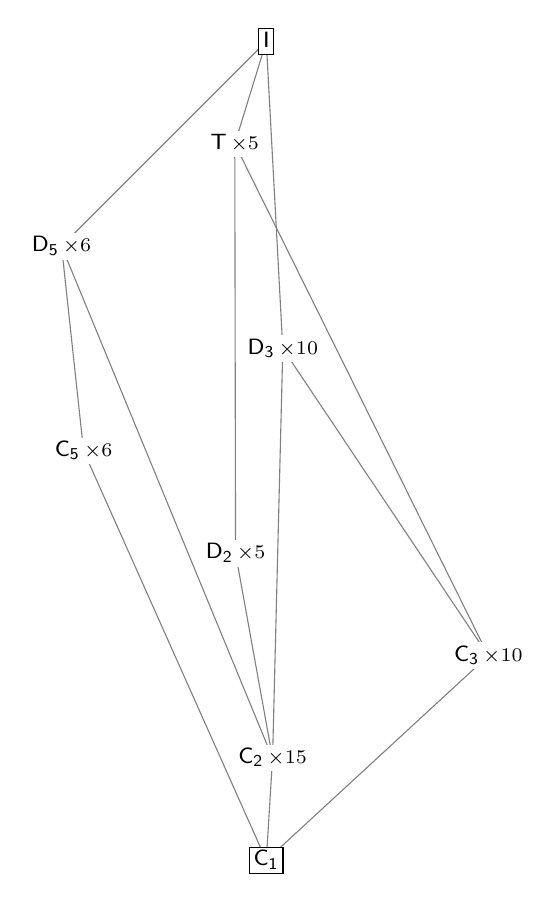
\begin{tikzpicture}[x=1cm, y=1.300cm,
  every node/.style={fill=white, font=\footnotesize, inner xsep=1.5pt, inner ysep=1.2pt, text height=5.6pt, text depth=1.6pt},
  normal/.style={draw, line width=0.4pt}, cover/.style={black!50, line width=0.4pt}]
\draw[cover] (0.00,0) -- (0.08,1);
\draw[cover] (0.00,0) -- (2.82,2);
\draw[cover] (0.00,0) -- (-2.32,4);
\draw[cover] (0.08,1) -- (-0.39,3);
\draw[cover] (0.08,1) -- (0.21,5);
\draw[cover] (0.08,1) -- (-2.60,6);
\draw[cover] (2.82,2) -- (0.21,5);
\draw[cover] (2.82,2) -- (-0.40,7);
\draw[cover] (-0.39,3) -- (-0.40,7);
\draw[cover] (-2.32,4) -- (-2.60,6);
\draw[cover] (0.21,5) -- (0.00,8);
\draw[cover] (-2.60,6) -- (0.00,8);
\draw[cover] (-0.40,7) -- (0.00,8);
\node[normal] (n00) at (0.00,0) {$\grp{C_{1}}$};
\node (n01) at (0.08,1) {$\grp{C_{2}}$\,\nconj{15}};
\node (n02) at (2.82,2) {$\grp{C_{3}}$\,\nconj{10}};
\node (n03) at (-0.39,3) {$\grp{D_{2}}$\,\nconj{5}};
\node (n04) at (-2.32,4) {$\grp{C_{5}}$\,\nconj{6}};
\node (n05) at (0.21,5) {$\grp{D_{3}}$\,\nconj{10}};
\node (n06) at (-2.60,6) {$\grp{D_{5}}$\,\nconj{6}};
\node (n07) at (-0.40,7) {$\grp{T}$\,\nconj{5}};
\node[normal] (n08) at (0.00,8) {$\grp{I}$};
\end{tikzpicture}
\end{center}
{\small\setlength{\fillwidth}{\textwidth}\addtolength{\fillwidth}{-12\tabcolsep}\setlength{\colwidth}{0pt}\cellmax{$\grp{C_{2}}$ $\samecls$ $\grp{D_{1}}$}\cellmax{subgrp}\cellmax{$\grp{C_{1}}$}\cellmax{$\grp{C_{3}}$}\cellmax{$\grp{C_{5}}$}\cellmax{$\grp{D_{2}}$}\cellmax{$\grp{D_{3}}$}\cellmax{$\grp{D_{5}}$}\cellmax{$\grp{I}$}\cellmax{$\grp{T}$}\addtolength{\fillwidth}{-\colwidth}\setlength{\colwidth}{0pt}\cellmax{order}\cellmax{10}\cellmax{12}\cellmax{60}\cellmax{1}\cellmax{2}\cellmax{3}\cellmax{4}\cellmax{5}\cellmax{6}\addtolength{\fillwidth}{-\colwidth}\setlength{\colwidth}{0pt}\cellmax{conjugates}\cellmax{10}\cellmax{15}\cellmax{1}\cellmax{5}\cellmax{6}\addtolength{\fillwidth}{-\colwidth}\setlength{\colwidth}{0pt}\cellmax{normal}\cellmax{yes}\cellmax{no}\addtolength{\fillwidth}{-\colwidth}\setlength{\colwidth}{0pt}\cellmax{$\grp{N}_{\hairsp \grp{I}}(\grp{H})$}\cellmax{$\grp{D_{2}}$}\cellmax{$\grp{D_{3}}$}\cellmax{$\grp{D_{5}}$}\cellmax{$\grp{I}$}\cellmax{$\grp{T}$}\addtolength{\fillwidth}{-\colwidth}\setlength{\colwidth}{0pt}\cellmax{$\grp{C}_{\hairsp \grp{I}}(\grp{H})$}\cellmax{$\grp{C_{1}}$}\cellmax{$\grp{C_{3}}$}\cellmax{$\grp{C_{5}}$}\cellmax{$\grp{D_{2}}$}\cellmax{$\grp{I}$}\addtolength{\fillwidth}{-\colwidth}\setlength{\colwidth}{0pt}\cellmax{$\cls{12C_{5}}$, $\cls{12C_{5}^{2}}$, $\cls{15C_{2}}$}\cellmax{$\cls{12C_{5}}$, $\cls{12C_{5}^{2}}$}\cellmax{$\cls{20C_{3}}$, $\cls{15C_{2}}$}\cellmax{classes}\cellmax{$\cls{15C_{2}}$}\cellmax{$\cls{20C_{3}}$}\cellmax{---}\cellmax{all}\fillcap\begin{longtable}{@{}lrrlll>{\RaggedRight\arraybackslash}p{\fillwidth}@{}}\toprule
subgrp & order & conjugates & normal & $\grp{N}_{\hairsp \grp{I}}(\grp{H})$ & $\grp{C}_{\hairsp \grp{I}}(\grp{H})$ & classes\\\midrule\endhead
\bottomrule\endfoot\endlastfoot
\href{C1.pdf}{$\grp{C_{1}}$} & 1 & 1 & yes & \href{I.pdf}{$\grp{I}$} & \href{I.pdf}{$\grp{I}$} & ---\\*
\href{C2.pdf}{$\grp{C_{2}}$} $\samecls$ \href{D1.pdf}{$\grp{D_{1}}$} & 2 & 15 & no & \href{D2.pdf}{$\grp{D_{2}}$} & \href{D2.pdf}{$\grp{D_{2}}$} & $\cls{15C_{2}}$\\
\href{C3.pdf}{$\grp{C_{3}}$} & 3 & 10 & no & \href{D3.pdf}{$\grp{D_{3}}$} & \href{C3.pdf}{$\grp{C_{3}}$} & $\cls{20C_{3}}$\\
\href{D2.pdf}{$\grp{D_{2}}$} & 4 & 5 & no & \href{T.pdf}{$\grp{T}$} & \href{D2.pdf}{$\grp{D_{2}}$} & $\cls{15C_{2}}$\\
\href{C5.pdf}{$\grp{C_{5}}$} & 5 & 6 & no & \href{D5.pdf}{$\grp{D_{5}}$} & \href{C5.pdf}{$\grp{C_{5}}$} & $\cls{12C_{5}}$, $\cls{12C_{5}^{2}}$\\
\href{D3.pdf}{$\grp{D_{3}}$} & 6 & 10 & no & \href{D3.pdf}{$\grp{D_{3}}$} & \href{C1.pdf}{$\grp{C_{1}}$} & $\cls{20C_{3}}$, $\cls{15C_{2}}$\\
\href{D5.pdf}{$\grp{D_{5}}$} & 10 & 6 & no & \href{D5.pdf}{$\grp{D_{5}}$} & \href{C1.pdf}{$\grp{C_{1}}$} & $\cls{12C_{5}}$, $\cls{12C_{5}^{2}}$, $\cls{15C_{2}}$\\
\href{T.pdf}{$\grp{T}$} & 12 & 5 & no & \href{T.pdf}{$\grp{T}$} & \href{C1.pdf}{$\grp{C_{1}}$} & $\cls{20C_{3}}$, $\cls{15C_{2}}$\\*
\href{I.pdf}{$\grp{I}$} & 60 & 1 & yes & \href{I.pdf}{$\grp{I}$} & \href{C1.pdf}{$\grp{C_{1}}$} & all\\
\bottomrule\end{longtable}}
\needspace{103pt}
\section{Descent of symmetry}\label{s:subduction}
Conventions: \href{../../CONVENTIONS.pdf}{CONVENTIONS.pdf}, sections \href{../../CONVENTIONS.pdf\#conv.12.2}{12.2} and \href{../../CONVENTIONS.pdf\#conv.12.4}{12.4}.
A column is a class of subgroups $\grp{H}$, in the order of the table of section~\ref{s:subgroups}. The row subgrp names it by its symbol, as in that table. The symbol links to the document of $\grp{H}$. The entry of row $\Gamma$ is $\restr{\Gamma}{\grp{H}}$, the restriction of $\Gamma$ along a monomorphism from the record of $\grp{H}$ onto the subgroup, as a sum of the irreps of $\grp{H}$. The monomorphism identifies the subgroup with its record, and $\grp{H}$ names both.
{\small\begin{longtable}{@{}lccccc@{}}\toprule
subgrp & \href{C2.pdf}{$\grp{C_{2}}$} & \href{C3.pdf}{$\grp{C_{3}}$} & \href{D2.pdf}{$\grp{D_{2}}$} & \href{C5.pdf}{$\grp{C_{5}}$} & \href{D3.pdf}{$\grp{D_{3}}$}\\\midrule\endhead
\bottomrule\endfoot\endlastfoot
$\irr{a}$ & $\irr{a}$ & $\irr{a}$ & $\irr{a}$ & $\irr{a}$ & $\irr{a}_{1}$\\*
$\irr{t}_{1}$ & $\irr{a}\oplus 2\,\irr{b}$ & $\irr{a}\oplus \conjpair{1}\irr{e}\oplus \conjpair{2}\irr{e}$ & $\irr{b}_{1}\oplus \irr{b}_{2}\oplus \irr{b}_{3}$ & $\irr{a}\oplus \conjpair{1}\irr{e}_{1}\oplus \conjpair{2}\irr{e}_{1}$ & $\irr{a}_{2}\oplus \irr{e}$\\*
$\irr{t}_{2}$ & $\irr{a}\oplus 2\,\irr{b}$ & $\irr{a}\oplus \conjpair{1}\irr{e}\oplus \conjpair{2}\irr{e}$ & $\irr{b}_{1}\oplus \irr{b}_{2}\oplus \irr{b}_{3}$ & $\irr{a}\oplus \conjpair{1}\irr{e}_{2}\oplus \conjpair{2}\irr{e}_{2}$ & $\irr{a}_{2}\oplus \irr{e}$\\*
$\irr{g}$ & $2\,\irr{a}\oplus 2\,\irr{b}$ & $2\,\irr{a}\oplus \conjpair{1}\irr{e}\oplus \conjpair{2}\irr{e}$ & $\irr{a}\oplus \irr{b}_{1}\oplus \irr{b}_{2}\oplus \irr{b}_{3}$ & $\conjpair{1}\irr{e}_{1}\oplus \conjpair{2}\irr{e}_{1}\oplus \conjpair{1}\irr{e}_{2}\oplus \conjpair{2}\irr{e}_{2}$ & $\irr{a}_{1}\oplus \irr{a}_{2}\oplus \irr{e}$\\*
$\irr{h}$ & $3\,\irr{a}\oplus 2\,\irr{b}$ & $\irr{a}\oplus 2\,\conjpair{1}\irr{e}\oplus 2\,\conjpair{2}\irr{e}$ & $2\,\irr{a}\oplus \irr{b}_{1}\oplus \irr{b}_{2}\oplus \irr{b}_{3}$ & $\irr{a}\oplus \conjpair{1}\irr{e}_{1}\oplus \conjpair{2}\irr{e}_{1}\oplus \conjpair{1}\irr{e}_{2}\oplus \conjpair{2}\irr{e}_{2}$ & $\irr{a}_{1}\oplus 2\,\irr{e}$\\
\bottomrule\end{longtable}}
{\small\begin{longtable}{@{}lcc@{}}\toprule
subgrp & \href{D5.pdf}{$\grp{D_{5}}$} & \href{T.pdf}{$\grp{T}$}\\\midrule\endhead
\bottomrule\endfoot\endlastfoot
$\irr{a}$ & $\irr{a}_{1}$ & $\irr{a}$\\*
$\irr{t}_{1}$ & $\irr{a}_{2}\oplus \irr{e}_{1}$ & $\irr{t}$\\*
$\irr{t}_{2}$ & $\irr{a}_{2}\oplus \irr{e}_{2}$ & $\irr{t}$\\*
$\irr{g}$ & $\irr{e}_{1}\oplus \irr{e}_{2}$ & $\irr{a}\oplus \irr{t}$\\*
$\irr{h}$ & $\irr{a}_{1}\oplus \irr{e}_{1}\oplus \irr{e}_{2}$ & $\conjpair{1}\irr{e}\oplus \conjpair{2}\irr{e}\oplus \irr{t}$\\
\bottomrule\end{longtable}}
\leavevmode\label{n:irrep.Delta}Read down a column, a table gives induction (Frobenius reciprocity): $\Gamma$ occurs in $\Ind{\grp{H}}{\grp{I}} \Lambda$ as often as $\Lambda$ occurs in the entry of row $\Gamma$. For every entry, the record holds the unitary matrix that carries $\restr{\Gamma}{\grp{H}}$ into the direct sum of the matrices of $\grp{H}$ (\texttt{subduction[].blocks}). For every class $\grp{H}$ it holds the left coset representatives (\texttt{transversal}). From both, $\Ind{\grp{H}}{\grp{I}} \Lambda$ and its intertwiners follow as in \href{../../CONVENTIONS.pdf}{CONVENTIONS.pdf}, section \href{../../CONVENTIONS.pdf\#conv.12.4}{12.4}.
\needspace{171pt}
\partbox{Permutation representations}
\section{Figures}\label{s:permutation}
Conventions: \href{../../CONVENTIONS.pdf}{CONVENTIONS.pdf}, sections \href{../../CONVENTIONS.pdf\#conv.12.4}{12.4} to \href{../../CONVENTIONS.pdf\#conv.12.6}{12.6}.
Every class of subgroups $\grp{H}$ is the stabilizer of a figure in space, the subgroup of the elements that carry it into itself. \label{n:local.orbit.size}The group $\grp{I}$ permutes the $N = [\grp{I} : \grp{H}]$ copies of the figure as it permutes the right cosets $\grp{H}\xi_j$, $j = 0, 1, \dots, N - 1$, ordered by the indices of their least elements $\xi_j$ ($\xi_0 = \cls{E}$). The copy $j$ is the figure moved by $\xi_j$. The matrices $P(g)$ of the defining representation of $\grp{I}$ (section~\ref{s:elements}) generate the copies, and the root point $\pointr_0$ of the figure moves to the point $\pointr_j = \pointr_0\, P(\xi_j)$ of the copy $j$. The element $g$ moves the copy $j$ to the copy $j'$, where $\grp{H}\xi_j g = \grp{H}\xi_{j'}$. \label{n:local.matrix.permutation}Its permutation matrix $D(g)$ has the one nonzero entry of row $j$ in column $j'$,
\begin{equation}\label{e:perm.matrix}\pointr_j\, P(g) = \pointr_{j'}, \qquad D(g)_{j,j'} = 1,\end{equation}
and it obeys $D(g)\, D(h) = D(gh)$. The record holds the coordinates of the points of every copy, the images $j'$ of every copy under every element and the table of marks (\href{../../CONVENTIONS.pdf}{CONVENTIONS.pdf}, sections \href{../../CONVENTIONS.pdf\#conv.12.5}{12.5} and \href{../../CONVENTIONS.pdf\#conv.12.6}{12.6}).
\leavevmode\label{n:head.figure}The figure of a class is the first of these whose stabilizer is $\grp{H}$: the point $\pointr_0$, the line through the origin along $\pointr_0$, a spin, a spinning arrow and a helix. Otherwise the figure is the least orbit of $\pointr_0$ under $\grp{H}$ whose stabilizer is $\grp{H}$, a segment, a polygon or a polyhedron. A spin is the axial vector $\pointr_0$, a sense of rotation about its line. A spinning arrow is the arrow $\pointr_0$ with a sense of rotation about itself, and a helix is the line along $\pointr_0$ with a handedness. These two figures are tried only when $\grp{H}$ has no improper element and $\grp{I}$ has one. The table lists the classes of subgroups in the order and with the names of the table of section~\ref{s:subgroups}. \label{n:head.site}A row gives $N$, the figure by its shape or number of points, the stabilizer of the point $\pointr_0$ (site), which tells the symmetry elements of $\grp{I}$ that the figure lies on, and $\pointr_0$. \label{n:head.vertices}The column vertices gives what the points of all the copies form (the tips of the arrows and spins, both ends of the lines and helices), with ${\times}k$ when $k > 1$ copies pass through each. \label{n:head.rank}The rank counts the classes of pairs of copies under $\grp{I}$, including that of a copy with itself. \label{n:head.cos}For a point, line or spin of rank at most 5, the column cos gives the cosine of the angle between two copies (of the acute angle, for lines) for each remaining class of pairs. \label{n:head.hand}The column hand gives 2 when $\grp{H}$ has no improper element and $\grp{I}$ has one, so that the rotations of $\grp{I}$ leave the copies in two classes, mirror images of each other. These classes are the left- and the right-handed copies of a chiral figure.
{\small\setlength{\tabcolsep}{4pt}\setlength{\fillwidth}{\textwidth}\addtolength{\fillwidth}{-16\tabcolsep}\setlength{\colwidth}{0pt}\cellmax{subgrp}\cellmax{$\grp{C_{1}}$}\cellmax{$\grp{C_{2}}$}\cellmax{$\grp{C_{3}}$}\cellmax{$\grp{C_{5}}$}\cellmax{$\grp{D_{2}}$}\cellmax{$\grp{D_{3}}$}\cellmax{$\grp{D_{5}}$}\cellmax{$\grp{I}$}\cellmax{$\grp{T}$}\addtolength{\fillwidth}{-\colwidth}\setlength{\colwidth}{0pt}\cellmax{10}\cellmax{12}\cellmax{15}\cellmax{20}\cellmax{30}\cellmax{60}\cellmax{$N$}\cellmax{1}\cellmax{5}\cellmax{6}\addtolength{\fillwidth}{-\colwidth}\setlength{\colwidth}{0pt}\cellmax{tetrahedron}\cellmax{figure}\cellmax{origin}\cellmax{point}\cellmax{line}\addtolength{\fillwidth}{-\colwidth}\setlength{\colwidth}{0pt}\cellmax{site}\cellmax{$\grp{C_{1}}$}\cellmax{$\grp{C_{2}}$}\cellmax{$\grp{C_{3}}$}\cellmax{$\grp{C_{5}}$}\cellmax{$\grp{I}$}\addtolength{\fillwidth}{-\colwidth}\setlength{\colwidth}{0pt}\cellmax{$(-1 - \goldenratio{}, \goldenratio{}, 1)$}\cellmax{$(1 - \goldenratio{}, -\goldenratio{}, 1)$}\cellmax{$(2 - \goldenratio{}, 0, 1)$}\cellmax{$(\goldenratio - 1, 0, \goldenratio{})$}\cellmax{$(0, 0, 0)$}\cellmax{$(1, 2, 4)$}\cellmax{$(\goldenratio{}, 0, 1)$}\cellmax{$\pointr_0$}\addtolength{\fillwidth}{-\colwidth}\setlength{\colwidth}{0pt}\cellmax{icosidodecahedron}\cellmax{dodecahedron}\cellmax{icosahedron}\cellmax{60 points}\cellmax{vertices}\cellmax{origin}\addtolength{\fillwidth}{-\colwidth}\setlength{\colwidth}{0pt}\cellmax{rank}\cellmax{16}\cellmax{60}\cellmax{1}\cellmax{2}\cellmax{3}\cellmax{4}\cellmax{6}\cellmax{8}\addtolength{\fillwidth}{-\colwidth}\setlength{\colwidth}{0pt}\cellmax{hand}\cellmax{}\addtolength{\fillwidth}{-\colwidth}\setlength{\colwidth}{0pt}\cellmax{${\tfrac{1}{5}(2\goldenratio - 1)}$, ${\tfrac{1}{5}(1 - 2\goldenratio)}$, ${-1}$}\cellmax{${\tfrac{1}{3}(2\goldenratio - 1)}$, ${\tfrac{1}{3}}$}\cellmax{${\tfrac{1}{5}(2\goldenratio - 1)}$}\cellmax{cos}\fillcap{\renewcommand{\arraystretch}{1.3}\begin{longtable}{@{}lrllllr>{\RaggedRight\arraybackslash}p{\fillwidth}r@{}}\toprule
subgrp & $N$ & figure & site & $\pointr_0$ & vertices & rank & cos & hand\\\midrule\endhead
\bottomrule\endfoot\endlastfoot
\href{C1.pdf}{$\grp{C_{1}}$} & 60 & point & \href{C1.pdf}{$\grp{C_{1}}$} & $(1, 2, 4)$ & 60 points & 60 &  & \\*
\href{C2.pdf}{$\grp{C_{2}}$} & 30 & point & \href{C2.pdf}{$\grp{C_{2}}$} & $(1 - \goldenratio{}, -\goldenratio{}, 1)$ & icosidodecahedron & 16 &  & \\
\href{C3.pdf}{$\grp{C_{3}}$} & 20 & point & \href{C3.pdf}{$\grp{C_{3}}$} & $(2 - \goldenratio{}, 0, 1)$ & dodecahedron & 8 &  & \\
\href{D2.pdf}{$\grp{D_{2}}$} & 15 & line & \href{C2.pdf}{$\grp{C_{2}}$} & $(-1 - \goldenratio{}, \goldenratio{}, 1)$ & icosidodecahedron & 6 &  & \\
\href{C5.pdf}{$\grp{C_{5}}$} & 12 & point & \href{C5.pdf}{$\grp{C_{5}}$} & $(\goldenratio{}, 0, 1)$ & icosahedron & 4 & ${\tfrac{1}{5}(2\goldenratio - 1)}$, ${\tfrac{1}{5}(1 - 2\goldenratio)}$, ${-1}$ & \\
\href{D3.pdf}{$\grp{D_{3}}$} & 10 & line & \href{C3.pdf}{$\grp{C_{3}}$} & $(2 - \goldenratio{}, 0, 1)$ & dodecahedron & 3 & ${\tfrac{1}{3}(2\goldenratio - 1)}$, ${\tfrac{1}{3}}$ & \\
\href{D5.pdf}{$\grp{D_{5}}$} & 6 & line & \href{C5.pdf}{$\grp{C_{5}}$} & $(\goldenratio{}, 0, 1)$ & icosahedron & 2 & ${\tfrac{1}{5}(2\goldenratio - 1)}$ & \\
\href{T.pdf}{$\grp{T}$} & 5 & tetrahedron & \href{C3.pdf}{$\grp{C_{3}}$} & $(\goldenratio - 1, 0, \goldenratio{})$ & dodecahedron & 2 &  & \\*
\href{I.pdf}{$\grp{I}$} & 1 & origin & \href{I.pdf}{$\grp{I}$} & $(0, 0, 0)$ & origin & 1 &  & \\
\bottomrule\end{longtable}}}
The copies of the figure of \href{T.pdf}{$\grp{T}$} form the compound of five tetrahedra, UC05 in the list of the uniform compounds [\href{../../../REFERENCES.pdf\#ref.Ski76}{Ski76}]. A uniform polyhedron has regular faces and all its vertices alike. Some points give orbits that are uniform polyhedra or regular polygons: a truncated dodecahedron, a truncated icosahedron, a rhombicosidodecahedron or a snub dodecahedron for \href{C1.pdf}{$\grp{C_{1}}$}.
\needspace{153pt}
\section{Decompositions}\label{s:decompositions}
Conventions: \href{../../CONVENTIONS.pdf}{CONVENTIONS.pdf}, sections \href{../../CONVENTIONS.pdf\#conv.12.4}{12.4} and \href{../../CONVENTIONS.pdf\#conv.12.5}{12.5}.
The kernel of the permutation representation of a class of subgroups is the subgroup of the elements that leave every copy in place. The decomposition is that of $D$, whose character at $g$ is the number of copies that $g$ leaves in place. An irrep occurs in $D$ as often as the trivial irrep of $\grp{H}$ occurs in its restriction to $\grp{H}$ (section~\ref{s:subduction}).
{\small\medmuskip=4mu plus 2mu\relax\setlength{\fillwidth}{\textwidth}\addtolength{\fillwidth}{-6\tabcolsep}\setlength{\colwidth}{0pt}\cellmax{subgrp}\cellmax{$\grp{C_{1}}$}\cellmax{$\grp{C_{2}}$}\cellmax{$\grp{C_{3}}$}\cellmax{$\grp{C_{5}}$}\cellmax{$\grp{D_{2}}$}\cellmax{$\grp{D_{3}}$}\cellmax{$\grp{D_{5}}$}\cellmax{$\grp{I}$}\cellmax{$\grp{T}$}\addtolength{\fillwidth}{-\colwidth}\setlength{\colwidth}{0pt}\cellmax{10}\cellmax{12}\cellmax{15}\cellmax{20}\cellmax{30}\cellmax{60}\cellmax{$N$}\cellmax{1}\cellmax{5}\cellmax{6}\addtolength{\fillwidth}{-\colwidth}\setlength{\colwidth}{0pt}\cellmax{kernel}\cellmax{$\grp{C_{1}}$}\cellmax{$\grp{I}$}\addtolength{\fillwidth}{-\colwidth}\setlength{\colwidth}{0pt}\cellmax{$\irr{a}\oplus 3\,\irr{t}_{1}\oplus 3\,\irr{t}_{2}\oplus 4\,\irr{g}\oplus 5\,\irr{h}$}\cellmax{$\irr{a}\oplus \irr{t}_{1}\oplus \irr{t}_{2}\oplus 2\,\irr{g}\oplus 3\,\irr{h}$}\cellmax{$\irr{a}\oplus \irr{t}_{1}\oplus \irr{t}_{2}\oplus 2\,\irr{g}\oplus \irr{h}$}\cellmax{$\irr{a}\oplus \irr{t}_{1}\oplus \irr{t}_{2}\oplus \irr{h}$}\cellmax{decomposition}\cellmax{$\irr{a}\oplus \irr{g}\oplus 2\,\irr{h}$}\cellmax{$\irr{a}\oplus \irr{g}\oplus \irr{h}$}\cellmax{$\irr{a}\oplus \irr{g}$}\cellmax{$\irr{a}\oplus \irr{h}$}\cellmax{$\irr{a}$}\fillcap\begin{longtable}{@{}lrl>{\RaggedRight\arraybackslash}p{\fillwidth}@{}}\toprule
subgrp & $N$ & kernel & decomposition\\\midrule\endhead
\bottomrule\endfoot\endlastfoot
\href{C1.pdf}{$\grp{C_{1}}$} & 60 & \href{C1.pdf}{$\grp{C_{1}}$} & $\irr{a}\oplus 3\,\irr{t}_{1}\oplus 3\,\irr{t}_{2}\oplus 4\,\irr{g}\oplus 5\,\irr{h}$\\*
\href{C2.pdf}{$\grp{C_{2}}$} & 30 & \href{C1.pdf}{$\grp{C_{1}}$} & $\irr{a}\oplus \irr{t}_{1}\oplus \irr{t}_{2}\oplus 2\,\irr{g}\oplus 3\,\irr{h}$\\
\href{C3.pdf}{$\grp{C_{3}}$} & 20 & \href{C1.pdf}{$\grp{C_{1}}$} & $\irr{a}\oplus \irr{t}_{1}\oplus \irr{t}_{2}\oplus 2\,\irr{g}\oplus \irr{h}$\\
\href{D2.pdf}{$\grp{D_{2}}$} & 15 & \href{C1.pdf}{$\grp{C_{1}}$} & $\irr{a}\oplus \irr{g}\oplus 2\,\irr{h}$\\
\href{C5.pdf}{$\grp{C_{5}}$} & 12 & \href{C1.pdf}{$\grp{C_{1}}$} & $\irr{a}\oplus \irr{t}_{1}\oplus \irr{t}_{2}\oplus \irr{h}$\\
\href{D3.pdf}{$\grp{D_{3}}$} & 10 & \href{C1.pdf}{$\grp{C_{1}}$} & $\irr{a}\oplus \irr{g}\oplus \irr{h}$\\
\href{D5.pdf}{$\grp{D_{5}}$} & 6 & \href{C1.pdf}{$\grp{C_{1}}$} & $\irr{a}\oplus \irr{h}$\\
\href{T.pdf}{$\grp{T}$} & 5 & \href{C1.pdf}{$\grp{C_{1}}$} & $\irr{a}\oplus \irr{g}$\\*
\href{I.pdf}{$\grp{I}$} & 1 & \href{I.pdf}{$\grp{I}$} & $\irr{a}$\\
\bottomrule\end{longtable}}
\needspace{103pt}
\section{Cycle types}\label{s:cycle_types}
Conventions: \href{../../CONVENTIONS.pdf}{CONVENTIONS.pdf}, section \href{../../CONVENTIONS.pdf\#conv.12.5}{12.5}.
\leavevmode\label{n:local.cycle.type}\label{n:local.cycle.length}\label{n:local.cycle.count}The entry in the row of a class of subgroups and the column of a class of elements is the cycle type of $j \mapsto j'$ for these elements, written $\ell^{c}$ for $c$ cycles of length $\ell$. The cycles of length 1 are the copies that the element leaves in place, whose number is the character of $D$. \label{n:local.cycles}\label{n:local.states}With $c(g)$ cycles in all, $g$ has the character $q^{c(g)}$ on the $q^N$ products of one of $q$ states of each copy (\href{../../CONVENTIONS.pdf}{CONVENTIONS.pdf}, section \href{../../CONVENTIONS.pdf\#conv.12.5}{12.5}).
{\small\setlength{\tabcolsep}{4pt}\begin{longtable}{@{}lrccccc@{}}\toprule
subgrp & $N$ & $\cls{E}$ & $\cls{12C_{5}}$ & $\cls{12C_{5}^{2}}$ & $\cls{20C_{3}}$ & $\cls{15C_{2}}$\\\midrule\endhead
\bottomrule\endfoot\endlastfoot
\href{C1.pdf}{$\grp{C_{1}}$} & 60 & $1^{60}$ & $5^{12}$ & $5^{12}$ & $3^{20}$ & $2^{30}$\\*
\href{C2.pdf}{$\grp{C_{2}}$} & 30 & $1^{30}$ & $5^{6}$ & $5^{6}$ & $3^{10}$ & $1^{2}\,2^{14}$\\*
\href{C3.pdf}{$\grp{C_{3}}$} & 20 & $1^{20}$ & $5^{4}$ & $5^{4}$ & $1^{2}\,3^{6}$ & $2^{10}$\\*
\href{D2.pdf}{$\grp{D_{2}}$} & 15 & $1^{15}$ & $5^{3}$ & $5^{3}$ & $3^{5}$ & $1^{3}\,2^{6}$\\*
\href{C5.pdf}{$\grp{C_{5}}$} & 12 & $1^{12}$ & $1^{2}\,5^{2}$ & $1^{2}\,5^{2}$ & $3^{4}$ & $2^{6}$\\*
\href{D3.pdf}{$\grp{D_{3}}$} & 10 & $1^{10}$ & $5^{2}$ & $5^{2}$ & $1\,3^{3}$ & $1^{2}\,2^{4}$\\*
\href{D5.pdf}{$\grp{D_{5}}$} & 6 & $1^{6}$ & $1\,5$ & $1\,5$ & $3^{2}$ & $1^{2}\,2^{2}$\\*
\href{T.pdf}{$\grp{T}$} & 5 & $1^{5}$ & $5$ & $5$ & $1^{2}\,3$ & $1\,2^{2}$\\
\bottomrule\end{longtable}}
\needspace{177pt}
\partbox{Angular momentum}
\section{Subduction from \texorpdfstring{$\grp{O(3)}$}{O(3)}}\label{s:subduction_o3}
Conventions: \href{../../CONVENTIONS.pdf}{CONVENTIONS.pdf}, section \href{../../CONVENTIONS.pdf\#conv.11}{11}.
\leavevmode\label{n:index.J}\label{n:index.parity}\label{n:function.multiplicity}The irrep $\irrJp{J}{p}$ of \href{O3.pdf}{$\grp{O(3)}$} has angular momentum $J$ and parity $p$ ($\ptag{g}$ for $p = +1$, $\ptag{u}$ for $p = -1$), and $b_\Gamma(J, p)$ is the multiplicity of $\Gamma$ in
\begin{equation}\label{e:o3}\restr{\irrJp{J}{p}}{\grp{I}} .\end{equation}
\leavevmode\label{n:index.increment}Each table gives $b_\Gamma(J, p)$ for $J \le 29$, and $b_\Gamma(J + 30, p) = b_\Gamma(J, p) + \Delta_\Gamma$ for every $J$, where $\Delta_\Gamma$ is the last row of the table of parity $p$.
\needspace{231pt}
\paragraph{Parity $\ptag{g}$ and $\ptag{u}$ ($p = \pm1$).}
Every element of $\grp{I}$ is a rotation, so the multiplicities do not depend on $p$ and one table gives both parities.
{\small\begin{longtable}{@{}rrrrrr@{\hspace{18pt}}rrrrrr@{\hspace{18pt}}rrrrrr@{}}\toprule
$J$ & $\irr{a}$ & $\irr{t}_{1}$ & $\irr{t}_{2}$ & $\irr{g}$ & $\irr{h}$ & $J$ & $\irr{a}$ & $\irr{t}_{1}$ & $\irr{t}_{2}$ & $\irr{g}$ & $\irr{h}$ & $J$ & $\irr{a}$ & $\irr{t}_{1}$ & $\irr{t}_{2}$ & $\irr{g}$ & $\irr{h}$\\\midrule\endhead
\bottomrule\endfoot\endlastfoot
0 & 1 & 0 & 0 & 0 & 0 & 11 & 0 & 2 & 1 & 1 & 2 & 22 & 1 & 2 & 2 & 3 & 4\\*
1 & 0 & 1 & 0 & 0 & 0 & 12 & 1 & 1 & 1 & 2 & 2 & 23 & 0 & 2 & 3 & 3 & 4\\*
2 & 0 & 0 & 0 & 0 & 1 & 13 & 0 & 1 & 2 & 2 & 2 & 24 & 1 & 2 & 2 & 4 & 4\\*
3 & 0 & 0 & 1 & 1 & 0 & 14 & 0 & 1 & 1 & 2 & 3 & 25 & 1 & 3 & 3 & 3 & 4\\*
4 & 0 & 0 & 0 & 1 & 1 & 15 & 1 & 2 & 2 & 2 & 2 & 26 & 1 & 3 & 2 & 3 & 5\\*
5 & 0 & 1 & 1 & 0 & 1 & 16 & 1 & 2 & 1 & 2 & 3 & 27 & 1 & 3 & 3 & 4 & 4\\*
6 & 1 & 1 & 0 & 1 & 1 & 17 & 0 & 2 & 2 & 2 & 3 & 28 & 1 & 2 & 3 & 4 & 5\\*
7 & 0 & 1 & 1 & 1 & 1 & 18 & 1 & 1 & 2 & 3 & 3 & 29 & 0 & 3 & 3 & 4 & 5\\*\noalign{\vskip 1.5pt}\multispan{6} & \multispan{6} & \multispan{6}\leaders\hrule height\cmidrulewidth\hfill\kern0pt\\*\noalign{\vskip 1.5pt}
8 & 0 & 0 & 1 & 1 & 2 & 19 & 0 & 2 & 2 & 3 & 3 & $\Delta_\Gamma$ & 1 & 3 & 3 & 4 & 5\\*
9 & 0 & 1 & 1 & 2 & 1 & 20 & 1 & 2 & 2 & 2 & 4 &  &  &  &  &  & \\*
10 & 1 & 1 & 1 & 1 & 2 & 21 & 1 & 3 & 2 & 3 & 3 &  &  &  &  &  & \\
\bottomrule\end{longtable}}
\needspace{110pt}
\section{Multiplicities and allowed \texorpdfstring{$m$}{m}}\label{s:multiplicities}
Conventions: \href{../../CONVENTIONS.pdf}{CONVENTIONS.pdf}, section \href{../../CONVENTIONS.pdf\#conv.14}{14}.
\leavevmode\label{n:function.generating}\label{n:index.generating.variable}\label{n:function.generating.numerator}The multiplicity $b_\Gamma(J) = b_\Gamma(J, (-1)^J)$ is the number of blocks of $\Gamma$ at $J$, with the generating function
\begin{equation}\label{e:gf}H_\Gamma(t) = \sum_{J\ge0} b_\Gamma(J)\,t^J = P_\Gamma(t)/((1-t^{6})(1-t^{10})).\end{equation}
\leavevmode\label{n:head.parity}The listed residues are the $m \bmod 2$ of the nonzero components of the vectors of $\Gamma$. A dash means no block of $\Gamma$ at that parity of $J$.
{\small\begin{longtable}{@{}llll@{}}\toprule
$\Gamma$ & $P_\Gamma(t)$ & $m \bmod 2$, $J$ even & $J$ odd\\\midrule\endhead
\bottomrule\endfoot\endlastfoot
$\irr{a}$ & $1 + t^{15}$ & 0 & 0\\*
$\irr{t}_{1}$ & $t + t^{5} + t^{6} + t^{9} + t^{10} + t^{14}$ & 0, 1 & 0, 1\\*
$\irr{t}_{2}$ & $t^{3} + t^{5} + t^{7} + t^{8} + t^{10} + t^{12}$ & 0, 1 & 0, 1\\*
$\irr{g}$ & $t^{3} + t^{4} + t^{6} + t^{7} + t^{8} + t^{9} + t^{11} + t^{12}$ & 0, 1 & 0, 1\\*
$\irr{h}$ & $t^{2} + t^{4} + t^{5} + t^{6} + t^{7} + t^{8} + t^{9} + t^{10} + t^{11} + t^{13}$ & 0, 1 & 0, 1\\
\bottomrule\end{longtable}}
\needspace{110pt}
\section{Symmetry-adapted bases}\label{s:bases}
Conventions: \href{../../CONVENTIONS.pdf}{CONVENTIONS.pdf}, sections \href{../../CONVENTIONS.pdf\#conv.14}{14} and \href{../../CONVENTIONS.pdf\#conv.14.2}{14.2} to \href{../../CONVENTIONS.pdf\#conv.14.4}{14.4}.
\leavevmode\label{n:index.m}\label{n:vector.ket}The kets $\jm{J}{m}$ are the spherical harmonics (the inversion acts as $(-1)^J$). \label{n:index.ketcoefficient}\label{n:vector.basis.symmetry}\label{n:index.ketweight}\label{n:index.total}A vector is listed by its coefficients $e_m$:
\begin{equation}\label{e:ket}v = \frac{1}{\sqrt{\mathrm{tot}}}\sum_m e_m\sqrt{F_m}\;\jm{J}{m},\qquad F_m = (J+m)!\,(J-m)!,\qquad \mathrm{tot} = \sum_m |e_m|^2F_m,\end{equation}
\leavevmode\label{n:index.factor.c}\label{n:index.multiplicity.copies}so the amplitude of $\jm{J}{m}$ is $e_m\sqrt{F_m/\mathrm{tot}}$, and a vector written $c\sum_m q_m\jm{J}{m}$ has $e_m = c\,q_m$.
The copies of $\Gamma$ at $J$ are orthonormal. \label{n:matrix.projector}In the coordinates $e_m$, $m = -J, -J+1, \dots, J$, their partner-1 vectors come from the vectors of the reduced row echelon basis of the range of
\begin{equation}\label{e:projector}P^\Gamma_{1,1} = \sum_g \conj{\repD{\Gamma}_{1,1}(g)}\,\irrJ{J}(g),\end{equation}
in the order of their lowest $m$. The index $\mult$ follows this order, and each partner-1 vector is its basis vector minus its projections on the copies before it (Gram--Schmidt). Partner $\intx$ is $P^\Gamma_{\intx,1}$ applied to partner 1.
The bases have 33 blocks and 121 vectors at $J = 0, 1, \dots, 10$. \label{n:head.vector}A row gives a vector of a block at $J$: the block's irrep and copy index $\mult$, the partner index $\intx$ and the vector. The full set $J = 0, 1, \dots, 60$ (993 blocks, 3721 vectors) is in \texttt{data/symmetry\symbol{95}adapted\symbol{95}bases/I/}. The repository holds $J \le 10$, and the release archive \texttt{I\symbol{95}J011-J060.tar} holds $J = 11, 12, \dots, 60$ and unpacks in the folder \texttt{rotation/} (README.md). A vector at $J = 4$ fills more than four lines, so the table stops at $J = 3$ (5 blocks, 16 vectors). The record (\texttt{subduction\symbol{95}basis.\allowbreak enumerated}) and the files also hold $J = 4, 5, \dots, 10$.
{\small\setlength{\emergencystretch}{2em}\setlength{\tabcolsep}{3pt}\setlength{\fillwidth}{\textwidth}\addtolength{\fillwidth}{-\dimexpr 6\tabcolsep+4pt\relax}\setlength{\colwidth}{0pt}\cellmax{$J$}\cellmax{0}\cellmax{1}\cellmax{2}\cellmax{3}\addtolength{\fillwidth}{-\colwidth}\setlength{\colwidth}{0pt}\cellmax{irrep}\cellmax{$\irr{t}_{1}$}\cellmax{$\irr{t}_{2}$}\cellmax{$\irr{a}$}\cellmax{$\irr{g}$}\cellmax{$\irr{h}$}\addtolength{\fillwidth}{-\colwidth}\setlength{\colwidth}{0pt}\cellmax{$\mult$}\cellmax{1}\addtolength{\fillwidth}{-\colwidth}\setlength{\colwidth}{0pt}\cellmax{$\intx$}\cellmax{1}\cellmax{2}\cellmax{3}\cellmax{4}\cellmax{5}\addtolength{\fillwidth}{-\colwidth}{\renewcommand{\arraystretch}{1.3}\begin{longtable}{@{}rlrr@{\hspace{4pt}}>{\RaggedRight\arraybackslash}p{\fillwidth}@{}}\toprule
$J$ & irrep & $\mult$ & $\intx$ & vector\\\midrule\endhead
\bottomrule\endfoot\endlastfoot
0 & $\irr{a}$ & 1 & 1 & $\jm{0}{0}$\\*
\grouprule{0pt}{\lightrulewidth}
1 & $\irr{t}_{1}$ & 1 & 1 & $\jm{1}{-1}$ $-\jm{1}{1}$\\*
1 & $\irr{t}_{1}$ & 1 & 2 & $\iunit{}\,(\jm{1}{-1}$ $+$ $\jm{1}{1})$\\*
1 & $\irr{t}_{1}$ & 1 & 3 & $\jm{1}{0}$\\
\grouprule{0pt}{\lightrulewidth}
2 & $\irr{h}$ & 1 & 1 & $59\,\jm{2}{-2}$ $+$ $(-176 + 12\sqrt{3} + 144\goldenratio + 28\sqrt{15} + 52\iunit - 6\iunit\sqrt{3} - 36\iunit\sqrt{5} - 14\iunit\sqrt{15})\,\jm{2}{-1}$ $+$ $(162 + 174\sqrt{3} - 36\goldenratio - 66\sqrt{15})\,\jm{2}{0}$ $+$ $(-176 + 12\sqrt{3} + 144\goldenratio + 28\sqrt{15} - 52\iunit + 6\iunit\sqrt{3} + 36\iunit\sqrt{5} + 14\iunit\sqrt{15})\,\jm{2}{1}$ $+$ $(6\sqrt{3} + 72\goldenratio + 14\sqrt{15} - 29)\,\jm{2}{2}$\\*
2 & $\irr{h}$ & 1 & 2 & $(108 - 2\sqrt{3} - 24\goldenratio + 15\sqrt{15})\rootunity{12}\,\jm{2}{-2}$ $+$ $(24 + 52\sqrt{3} - 84\goldenratio - 36\sqrt{15})\rootunity{3}\,\jm{2}{-1}$ $+$ $(24 - 66\sqrt{3} - 84\goldenratio - 36\sqrt{15})\rootunity{12}\,\jm{2}{0}$ $+$ $(-52\sqrt{3} + 84\goldenratio + 36\sqrt{15} - 24)\rootunity{3}\,\jm{2}{1}$ $+$ $(132 + 50\sqrt{3} - 108\goldenratio - 21\sqrt{15})\rootunity{12}\,\jm{2}{2}$\\*
2 & $\irr{h}$ & 1 & 3 & $\tfrac{1}{2}(3\sqrt{3} + 36\goldenratio + 7\sqrt{15} - 44)\rootunity{3}^{2}\,\jm{2}{-2}$ $+$ $\tfrac{1}{2}(32 - 29\sqrt{3} + 6\goldenratio + 11\sqrt{15} + 17\iunit + 23\iunit\sqrt{3} - 39\iunit\sqrt{5} - 25\iunit\sqrt{15})\,\jm{2}{-1}$ $+$ $\tfrac{1}{2}(56 + 23\sqrt{3} - 78\goldenratio - 25\sqrt{15} - 35\iunit + 29\iunit\sqrt{3} - 3\iunit\sqrt{5} - 11\iunit\sqrt{15})\,\jm{2}{1}$ $+$ $\tfrac{1}{2}(44 - 3\sqrt{3} - 36\goldenratio - 7\sqrt{15})\rootunity{3}^{2}\,\jm{2}{2}$\\*
2 & $\irr{h}$ & 1 & 4 & $(-50\sqrt{3} + 108\goldenratio + 21\sqrt{15} - 132)\iunit{}\,\jm{2}{-2}$ $+$ $(-52\sqrt{3} + 84\goldenratio + 36\sqrt{15} - 24)\,\jm{2}{-1}$ $+$ $(66\sqrt{3} + 84\goldenratio + 36\sqrt{15} - 24)\iunit{}\,\jm{2}{0}$ $+$ $(24 + 52\sqrt{3} - 84\goldenratio - 36\sqrt{15})\,\jm{2}{1}$ $+$ $(2\sqrt{3} + 24\goldenratio - 15\sqrt{15} - 108)\iunit{}\,\jm{2}{2}$\\*
2 & $\irr{h}$ & 1 & 5 & $(29 - 6\sqrt{3} - 72\goldenratio - 14\sqrt{15})\rootunity{3}\,\jm{2}{-2}$ $+$ $(76 - 32\sqrt{3} - 30\goldenratio + 4\sqrt{15} - 8\iunit - 49\iunit\sqrt{3} + 60\iunit\sqrt{5} + 43\iunit\sqrt{15})\,\jm{2}{-1}$ $+$ $(-174\sqrt{3} + 36\goldenratio + 66\sqrt{15} - 162)\rootunity{3}\,\jm{2}{0}$ $+$ $(100 + 20\sqrt{3} - 114\goldenratio - 32\sqrt{15} + 44\iunit - 55\iunit\sqrt{3} + 24\iunit\sqrt{5} + 29\iunit\sqrt{15})\,\jm{2}{1}$ $-59\rootunity{3}\,\jm{2}{2}$\\
\grouprule{0pt}{\lightrulewidth}
3 & $\irr{t}_{2}$ & 1 & 1 & $\jm{3}{-3}$ $+$ $(21 - 12\goldenratio{})\,\jm{3}{-1}$ $+$ $(12\goldenratio - 21)\,\jm{3}{1}$ $-\jm{3}{3}$\\*
3 & $\irr{t}_{2}$ & 1 & 2 & $(5 - 3\goldenratio)\iunit{}\,\jm{3}{-3}$ $+$ $(3\goldenratio - 9)\iunit{}\,\jm{3}{-1}$ $+$ $(3\goldenratio - 9)\iunit{}\,\jm{3}{1}$ $+$ $(5 - 3\goldenratio)\iunit{}\,\jm{3}{3}$\\*
3 & $\irr{t}_{2}$ & 1 & 3 & $(3\goldenratio - 6)\,\jm{3}{-2}$ $+$ $(6\goldenratio - 8)\,\jm{3}{0}$ $+$ $(3\goldenratio - 6)\,\jm{3}{2}$\\
3 & $\irr{g}$ & 1 & 1 & $\jm{3}{-3}$ $+$ $(6 - 6\goldenratio + 4\sin\tfrac{4\pi}{5})\,\jm{3}{-2}$ $+$ $(27 - 14\goldenratio - 20\sin\tfrac{2\pi}{5} + 20\sin\tfrac{4\pi}{5})\,\jm{3}{-1}$ $+$ $(44 - 28\goldenratio - 32\sin\tfrac{2\pi}{5} + 56\sin\tfrac{4\pi}{5})\,\jm{3}{0}$ $+$ $(23 - 16\goldenratio - 8\sin\tfrac{2\pi}{5} + 24\sin\tfrac{4\pi}{5})\,\jm{3}{1}$ $+$ $(18\goldenratio + 16\sin\tfrac{2\pi}{5} - 28\sin\tfrac{4\pi}{5} - 26)\,\jm{3}{2}$ $+$ $(5 - 2\goldenratio - 4\sin\tfrac{2\pi}{5} + 4\sin\tfrac{4\pi}{5})\,\jm{3}{3}$\\*
3 & $\irr{g}$ & 1 & 2 & $(6\goldenratio + 8\sin\tfrac{2\pi}{5} - 12\sin\tfrac{4\pi}{5} - 11)\rootunity{5}^{3}\,\jm{3}{-3}$ $+$ $(18 - 14\goldenratio - 8\sin\tfrac{2\pi}{5} + 20\sin\tfrac{4\pi}{5})\rootunity{5}^{3}\,\jm{3}{-2}$ $+$ $(12\goldenratio + 12\sin\tfrac{2\pi}{5} - 16\sin\tfrac{4\pi}{5} - 21)\rootunity{5}^{3}\,\jm{3}{-1}$ $+$ $(4\goldenratio + 16\sin\tfrac{2\pi}{5} - 8\sin\tfrac{4\pi}{5} - 12)\rootunity{5}^{3}\,\jm{3}{0}$ $+$ $(18\goldenratio + 16\sin\tfrac{2\pi}{5} - 28\sin\tfrac{4\pi}{5} - 29)\rootunity{5}^{3}\,\jm{3}{1}$ $+$ $(10\goldenratio + 8\sin\tfrac{2\pi}{5} - 12\sin\tfrac{4\pi}{5} - 14)\rootunity{5}^{3}\,\jm{3}{2}$ $+$ $(5 - 4\goldenratio - 4\sin\tfrac{2\pi}{5} + 8\sin\tfrac{4\pi}{5})\rootunity{5}^{3}\,\jm{3}{3}$\\*
3 & $\irr{g}$ & 1 & 3 & $(5 - 4\goldenratio - 4\sin\tfrac{2\pi}{5} + 8\sin\tfrac{4\pi}{5})\rootunity{5}\,\jm{3}{-3}$ $+$ $(14 - 10\goldenratio - 8\sin\tfrac{2\pi}{5} + 12\sin\tfrac{4\pi}{5})\rootunity{5}\,\jm{3}{-2}$ $+$ $(18\goldenratio + 16\sin\tfrac{2\pi}{5} - 28\sin\tfrac{4\pi}{5} - 29)\rootunity{5}\,\jm{3}{-1}$ $+$ $(12 - 4\goldenratio - 16\sin\tfrac{2\pi}{5} + 8\sin\tfrac{4\pi}{5})\rootunity{5}\,\jm{3}{0}$ $+$ $(12\goldenratio + 12\sin\tfrac{2\pi}{5} - 16\sin\tfrac{4\pi}{5} - 21)\rootunity{5}\,\jm{3}{1}$ $+$ $(14\goldenratio + 8\sin\tfrac{2\pi}{5} - 20\sin\tfrac{4\pi}{5} - 18)\rootunity{5}\,\jm{3}{2}$ $+$ $(6\goldenratio + 8\sin\tfrac{2\pi}{5} - 12\sin\tfrac{4\pi}{5} - 11)\rootunity{5}\,\jm{3}{3}$\\*
3 & $\irr{g}$ & 1 & 4 & $(-2 + 4\iunit - 2\rootunity{5}^{3} + 3\rootunity{5}^{4} + 2\rootunity{20} - 4\rootunity{20}^{3})\,\jm{3}{-3}$ $+$ $(26 - 18\goldenratio - 16\sin\tfrac{2\pi}{5} + 28\sin\tfrac{4\pi}{5})\rootunity{5}^{4}\,\jm{3}{-2}$ $+$ $(23 - 16\goldenratio - 8\sin\tfrac{2\pi}{5} + 24\sin\tfrac{4\pi}{5})\rootunity{5}^{4}\,\jm{3}{-1}$ $+$ $(28\goldenratio + 32\sin\tfrac{2\pi}{5} - 56\sin\tfrac{4\pi}{5} - 44)\rootunity{5}^{4}\,\jm{3}{0}$ $+$ $(-14 + 20\iunit - 14\rootunity{5}^{3} + 13\rootunity{5}^{4} + 10\rootunity{20} - 20\rootunity{20}^{3})\,\jm{3}{1}$ $+$ $(6 + 6\rootunity{5}^{3} + 2\rootunity{20}^{3} + 2\rootunity{20}^{9})\,\jm{3}{2}$ $+$ $\rootunity{5}^{4}\,\jm{3}{3}$\\
\bottomrule\end{longtable}}}
\needspace{220pt}
\partbox{Tensors}
\section{\texorpdfstring{$\orbital{s}$, $\orbital{p}$, $\orbital{d}$, $\orbital{f}$}{s, p, d, f} functions}\label{s:orbitals}
Conventions: \href{../../CONVENTIONS.pdf}{CONVENTIONS.pdf}, section \href{../../CONVENTIONS.pdf\#conv.13}{13}.
\leavevmode\label{n:head.function}A function is a real solid harmonic $\orbital{s}$, $\orbital{p}$, $\orbital{d}$ or $\orbital{f}$, of degree 0 to 3 with coprime integer coefficients, or a component $\orbital{R}_{x}$, $\orbital{R}_{y}$, $\orbital{R}_{z}$ of an axial vector. \label{n:head.polynomial}\label{n:head.irreps}A row gives the function, its polynomial in $x$, $y$ and $z$, and the irreps of its nonzero isotypic components.
{\small\begin{longtable}{@{}lll@{}}\toprule
function & polynomial & irreps\\\midrule\endhead
\bottomrule\endfoot\endlastfoot
$\orbital{s}$ & $1$ & $\irr{a}$\\*
$\orbital{p}_{x}$ & $x$ & $\irr{t}_{1}$\\
$\orbital{p}_{y}$ & $y$ & $\irr{t}_{1}$\\
$\orbital{p}_{z}$ & $z$ & $\irr{t}_{1}$\\
$\orbital{d}_{z^2}$ & $-x^{2} - y^{2} + 2z^{2}$ & $\irr{h}$\\
$\orbital{d}_{x^2-y^2}$ & $x^{2} - y^{2}$ & $\irr{h}$\\
$\orbital{d}_{xy}$ & $xy$ & $\irr{h}$\\
$\orbital{d}_{yz}$ & $yz$ & $\irr{h}$\\
$\orbital{d}_{zx}$ & $xz$ & $\irr{h}$\\
$\orbital{f}_{z^3}$ & $-3x^{2}z - 3y^{2}z + 2z^{3}$ & $\irr{t}_{2}$, $\irr{g}$ (not one irrep)\\
$\orbital{f}_{xz^2}$ & $-x^{3} - xy^{2} + 4xz^{2}$ & $\irr{t}_{2}$, $\irr{g}$ (not one irrep)\\
$\orbital{f}_{yz^2}$ & $-x^{2}y - y^{3} + 4yz^{2}$ & $\irr{t}_{2}$, $\irr{g}$ (not one irrep)\\
$\orbital{f}_{z(x^2-y^2)}$ & $x^{2}z - y^{2}z$ & $\irr{t}_{2}$, $\irr{g}$ (not one irrep)\\
$\orbital{f}_{xyz}$ & $xyz$ & $\irr{g}$\\
$\orbital{f}_{x(x^2-3y^2)}$ & $x^{3} - 3xy^{2}$ & $\irr{t}_{2}$, $\irr{g}$ (not one irrep)\\
$\orbital{f}_{y(3x^2-y^2)}$ & $3x^{2}y - y^{3}$ & $\irr{t}_{2}$, $\irr{g}$ (not one irrep)\\
$\orbital{R}_{x}$ & $x$ & $\irr{t}_{1}$\\
$\orbital{R}_{y}$ & $y$ & $\irr{t}_{1}$\\*
$\orbital{R}_{z}$ & $z$ & $\irr{t}_{1}$\\
\bottomrule\end{longtable}}
\needspace{247pt}
\needspace{103pt}
\section{Tensor spaces}\label{s:tensor_spaces}
Conventions: \href{../../CONVENTIONS.pdf}{CONVENTIONS.pdf}, section \href{../../CONVENTIONS.pdf\#conv.13}{13}.
\leavevmode\label{n:head.name}\label{n:head.description}\label{n:head.dim}\label{n:head.decomposition}A row is a space of Cartesian tensors, with its Jahn symbol (name), its description in words, its dimension (dim) and the irreps of $\grp{I}$ that it carries, with their multiplicities (decomposition). \label{n:label.jahn}The same symbol names the space in the isotypic components (V a polar vector, e an axial factor, a power the number of factors, brackets their symmetrized product). The descriptions name the symmetric polar tensors of a rank (the homogeneous polynomials of that degree), the axial vectors and the symmetric axial tensors of ranks 2 (optical activity) and 3. The elastic stiffness tensors are symmetric in their first two indices, in their last two and under the exchange of the two pairs. The photoelastic tensors are symmetric in their first two and in their last two indices, as are the electrostriction and the quadratic electro-optic tensors. The piezoelectric tensors are symmetric in their last two indices, the third-harmonic susceptibilities in their last three and the electrogyration tensors, which are axial, in their first two. The general polar tensors of rank 4 have no symmetry.
{\small\setlength{\fillwidth}{\textwidth}\addtolength{\fillwidth}{-6\tabcolsep}\setlength{\colwidth}{0pt}\cellmax{$\jahn{[[V^{2}]^{2}]}$}\cellmax{$\jahn{e[V^{2}]V}$}\cellmax{$\jahn{V[V^{2}]}$}\cellmax{$\jahn{V[V^{3}]}$}\cellmax{$\jahn{[V^{2}]^{2}}$}\cellmax{$\jahn{e[V^{2}]}$}\cellmax{$\jahn{e[V^{3}]}$}\cellmax{$\jahn{[V^{2}]}$}\cellmax{$\jahn{[V^{3}]}$}\cellmax{$\jahn{[V^{4}]}$}\cellmax{name}\cellmax{$\jahn{V^{0}}$}\cellmax{$\jahn{V^{4}}$}\cellmax{$\jahn{eV}$}\cellmax{$\jahn{V}$}\addtolength{\fillwidth}{-\colwidth}\setlength{\colwidth}{0pt}\cellmax{third-harmonic susceptibilities}\cellmax{symmetric axial tensors, rank 2}\cellmax{symmetric axial tensors, rank 3}\cellmax{symmetric polar tensors, rank 2}\cellmax{symmetric polar tensors, rank 3}\cellmax{symmetric polar tensors, rank 4}\cellmax{general polar tensors, rank 4}\cellmax{elastic stiffness tensors}\cellmax{electrogyration tensors}\cellmax{piezoelectric tensors}\cellmax{photoelastic tensors}\cellmax{axial vectors}\cellmax{polar vectors}\cellmax{description}\cellmax{scalars}\addtolength{\fillwidth}{-\colwidth}\setlength{\colwidth}{0pt}\cellmax{dim}\cellmax{10}\cellmax{15}\cellmax{18}\cellmax{21}\cellmax{30}\cellmax{36}\cellmax{81}\cellmax{1}\cellmax{3}\cellmax{6}\addtolength{\fillwidth}{-\colwidth}\setlength{\colwidth}{0pt}\cellmax{$3\,\irr{a} \oplus\allowbreak 6\,\irr{t}_{1} \oplus\allowbreak 3\,\irr{t}_{2} \oplus\allowbreak 4\,\irr{g} \oplus\allowbreak 7\,\irr{h}$}\cellmax{$2\,\irr{a} \oplus\allowbreak \irr{t}_{1} \oplus\allowbreak \irr{t}_{2} \oplus\allowbreak 2\,\irr{g} \oplus\allowbreak 4\,\irr{h}$}\cellmax{$\irr{a} \oplus\allowbreak \irr{t}_{1} \oplus\allowbreak \irr{t}_{2} \oplus\allowbreak 2\,\irr{g} \oplus\allowbreak 3\,\irr{h}$}\cellmax{$2\,\irr{t}_{1} \oplus\allowbreak \irr{t}_{2} \oplus\allowbreak \irr{g} \oplus\allowbreak \irr{h}$}\cellmax{decomposition}\cellmax{$2\,\irr{a} \oplus\allowbreak \irr{g} \oplus\allowbreak 3\,\irr{h}$}\cellmax{$\irr{t}_{1} \oplus\allowbreak \irr{t}_{2} \oplus\allowbreak \irr{g}$}\cellmax{$\irr{a} \oplus\allowbreak \irr{g} \oplus\allowbreak 2\,\irr{h}$}\cellmax{$\irr{a} \oplus\allowbreak \irr{h}$}\cellmax{$\irr{t}_{1}$}\cellmax{$\irr{a}$}\fillcap\begin{longtable}{@{}llr>{\RaggedRight\arraybackslash}p{\fillwidth}@{}}\toprule
name & description & dim & decomposition\\\midrule\endhead
\bottomrule\endfoot\endlastfoot
$\jahn{V^{0}}$ & scalars & 1 & $\irr{a}$\\*
$\jahn{V}$ & polar vectors & 3 & $\irr{t}_{1}$\\
$\jahn{[V^{2}]}$ & symmetric polar tensors, rank 2 & 6 & $\irr{a} \oplus\allowbreak \irr{h}$\\
$\jahn{[V^{3}]}$ & symmetric polar tensors, rank 3 & 10 & $\irr{t}_{1} \oplus\allowbreak \irr{t}_{2} \oplus\allowbreak \irr{g}$\\
$\jahn{[V^{4}]}$ & symmetric polar tensors, rank 4 & 15 & $\irr{a} \oplus\allowbreak \irr{g} \oplus\allowbreak 2\,\irr{h}$\\
$\jahn{eV}$ & axial vectors & 3 & $\irr{t}_{1}$\\
$\jahn{e[V^{2}]}$ & symmetric axial tensors, rank 2 & 6 & $\irr{a} \oplus\allowbreak \irr{h}$\\
$\jahn{e[V^{3}]}$ & symmetric axial tensors, rank 3 & 10 & $\irr{t}_{1} \oplus\allowbreak \irr{t}_{2} \oplus\allowbreak \irr{g}$\\
$\jahn{[[V^{2}]^{2}]}$ & elastic stiffness tensors & 21 & $2\,\irr{a} \oplus\allowbreak \irr{g} \oplus\allowbreak 3\,\irr{h}$\\
$\jahn{V[V^{2}]}$ & piezoelectric tensors & 18 & $2\,\irr{t}_{1} \oplus\allowbreak \irr{t}_{2} \oplus\allowbreak \irr{g} \oplus\allowbreak \irr{h}$\\
$\jahn{e[V^{2}]V}$ & electrogyration tensors & 18 & $2\,\irr{t}_{1} \oplus\allowbreak \irr{t}_{2} \oplus\allowbreak \irr{g} \oplus\allowbreak \irr{h}$\\
$\jahn{[V^{2}]^{2}}$ & photoelastic tensors & 36 & $2\,\irr{a} \oplus\allowbreak \irr{t}_{1} \oplus\allowbreak \irr{t}_{2} \oplus\allowbreak 2\,\irr{g} \oplus\allowbreak 4\,\irr{h}$\\
$\jahn{V[V^{3}]}$ & third-harmonic susceptibilities & 30 & $\irr{a} \oplus\allowbreak \irr{t}_{1} \oplus\allowbreak \irr{t}_{2} \oplus\allowbreak 2\,\irr{g} \oplus\allowbreak 3\,\irr{h}$\\*
$\jahn{V^{4}}$ & general polar tensors, rank 4 & 81 & $3\,\irr{a} \oplus\allowbreak 6\,\irr{t}_{1} \oplus\allowbreak 3\,\irr{t}_{2} \oplus\allowbreak 4\,\irr{g} \oplus\allowbreak 7\,\irr{h}$\\
\bottomrule\end{longtable}}
\needspace{235pt}
\needspace{103pt}
\section{Isotypic components}\label{s:isotypic}
Conventions: \href{../../CONVENTIONS.pdf}{CONVENTIONS.pdf}, section \href{../../CONVENTIONS.pdf\#conv.13}{13}.
\leavevmode\label{n:head.multiplicity}A row is an isotypic component, with the Jahn symbol of its space (name, as in the tensor spaces), its irrep, the multiplicity of the irrep in the space (mult.) and the component's dimension (dim). \label{n:head.coefficients}\label{n:head.basis}It also gives the field of the coefficients of its basis, rational or cyclotomic, and its reduced row echelon basis. \label{n:matrix.elastic}\label{n:matrix.piezoelectric}\label{n:matrix.electrogyration}\label{n:matrix.photoelastic}\label{n:matrix.susceptibility}A basis tensor of the elastic, piezoelectric, electrogyration or photoelastic tensors or of the third-harmonic susceptibilities is a combination of their coordinates, in this order, $c_{11}, \dots, c_{66}$, $d_{11}, \dots, d_{36}$, $\mathnormal{g}_{11}, \dots, \mathnormal{g}_{63}$, $p_{11}, \dots, p_{66}$ or $\chi^{(3)}_{1111}, \dots, \chi^{(3)}_{3333}$ (\href{../../CONVENTIONS.pdf}{CONVENTIONS.pdf}, section \href{../../CONVENTIONS.pdf\#conv.13}{13}). Each coordinate stands for the tensor with that coordinate 1 and every other coordinate 0. The symmetric axial tensors of ranks 2 and 3, the electrogyration and photoelastic tensors and the third-harmonic susceptibilities have only the trivial irrep's row, where they contain that irrep. The general polar tensors of rank 4 have none.
{\small\setlength{\fillwidth}{\textwidth}\addtolength{\fillwidth}{-10\tabcolsep}\setlength{\colwidth}{0pt}\cellmax{$\jahn{[[V^{2}]^{2}]}$}\cellmax{$\jahn{V[V^{2}]}$}\cellmax{$\jahn{V[V^{3}]}$}\cellmax{$\jahn{[V^{2}]^{2}}$}\cellmax{$\jahn{e[V^{2}]}$}\cellmax{$\jahn{[V^{2}]}$}\cellmax{$\jahn{[V^{3}]}$}\cellmax{$\jahn{[V^{4}]}$}\cellmax{name}\cellmax{$\jahn{V^{0}}$}\cellmax{$\jahn{eV}$}\cellmax{$\jahn{V}$}\addtolength{\fillwidth}{-\colwidth}\setlength{\colwidth}{0pt}\cellmax{irrep}\cellmax{$\irr{t}_{1}$}\cellmax{$\irr{t}_{2}$}\cellmax{$\irr{a}$}\cellmax{$\irr{g}$}\cellmax{$\irr{h}$}\addtolength{\fillwidth}{-\colwidth}\setlength{\colwidth}{0pt}\cellmax{mult.}\cellmax{1}\cellmax{2}\cellmax{3}\addtolength{\fillwidth}{-\colwidth}\setlength{\colwidth}{0pt}\cellmax{dim}\cellmax{10}\cellmax{15}\cellmax{1}\cellmax{2}\cellmax{3}\cellmax{4}\cellmax{5}\cellmax{6}\addtolength{\fillwidth}{-\colwidth}\setlength{\colwidth}{0pt}\cellmax{coefficients}\cellmax{cyclotomic}\cellmax{rational}\addtolength{\fillwidth}{-\colwidth}\begin{longtable}{@{}llrrl>{\RaggedRight\arraybackslash}p{\fillwidth}@{}}\toprule
name & irrep & mult. & dim & coefficients & basis\\\midrule\endhead
\bottomrule\endfoot\endlastfoot
$\jahn{V^{0}}$ & $\irr{a}$ & 1 & 1 & rational & $1$\\*
$\jahn{V}$ & $\irr{t}_{1}$ & 1 & 3 & rational & $x$, $y$, $z$\\
$\jahn{[V^{2}]}$ & $\irr{a}$ & 1 & 1 & rational & $x^{2} + y^{2} + z^{2}$\\
$\jahn{[V^{2}]}$ & $\irr{h}$ & 1 & 5 & rational & $x^{2} - z^{2}$, $xy$, $xz$, $y^{2} - z^{2}$, $yz$\\
$\jahn{[V^{3}]}$ & $\irr{t}_{1}$ & 1 & 3 & rational & $x^{3} + xy^{2} + xz^{2}$, $x^{2}y + y^{3} + yz^{2}$, $x^{2}z + y^{2}z + z^{3}$\\
$\jahn{[V^{3}]}$ & $\irr{t}_{2}$ & 1 & 3 & cyclotomic & $x^{3} - 3\goldenratio{}\,xy^{2} + \left(3\goldenratio - 3\right)xz^{2}$, $3x^{2}y + \goldenratio{}\,y^{3} - \left(3 + 3\goldenratio{}\right)yz^{2}$, $3x^{2}z + \left(3\goldenratio - 6\right)y^{2}z + \left(1 - \goldenratio{}\right)z^{3}$\\
$\jahn{[V^{3}]}$ & $\irr{g}$ & 1 & 4 & cyclotomic & $x^{3} + \left(\goldenratio - 2\right)xy^{2} - \left(1 + \goldenratio{}\right)xz^{2}$, $x^{2}y + \left(\goldenratio - 2\right)y^{3} + \left(5 - 3\goldenratio{}\right)yz^{2}$, $x^{2}z + \left(2 + 3\goldenratio{}\right)y^{2}z - \left(1 + \goldenratio{}\right)z^{3}$, $xyz$\\
$\jahn{[V^{4}]}$ & $\irr{a}$ & 1 & 1 & rational & $x^{4} + 2x^{2}y^{2} + 2x^{2}z^{2} + y^{4} + 2y^{2}z^{2} + z^{4}$\\
$\jahn{[V^{4}]}$ & $\irr{g}$ & 1 & 4 & cyclotomic & $x^{4} - 3x^{2}y^{2} - 3x^{2}z^{2} + y^{4} - 3y^{2}z^{2} + z^{4}$, $x^{3}y + \left(\goldenratio - 2\right)xy^{3} + \left(3 - 3\goldenratio{}\right)xyz^{2}$, $x^{3}z + 3\goldenratio{}\,xy^{2}z - \left(1 + \goldenratio{}\right)xz^{3}$, $3x^{2}yz - \goldenratio{}\,y^{3}z + \left(\goldenratio - 1\right)yz^{3}$\\
$\jahn{[V^{4}]}$ & $\irr{h}$ & 2 & 10 & cyclotomic & $x^{4} - z^{4}$, $x^{3}y + \goldenratio{}\,xyz^{2}$, $x^{3}z + \left(2 - \goldenratio{}\right)xz^{3}$, $x^{2}y^{2} - y^{2}z^{2}$, $x^{2}yz - \goldenratio{}\,yz^{3}$, $x^{2}z^{2} - y^{2}z^{2}$, $xy^{3} + \left(1 - \goldenratio{}\right)xyz^{2}$, $xy^{2}z + \left(\goldenratio - 1\right)xz^{3}$, $y^{4} - z^{4}$, $y^{3}z + \left(1 + \goldenratio{}\right)yz^{3}$\\
$\jahn{eV}$ & $\irr{t}_{1}$ & 1 & 3 & rational & $x$, $y$, $z$\\
$\jahn{e[V^{2}]}$ & $\irr{a}$ & 1 & 1 & rational & $x^{2} + y^{2} + z^{2}$\\
$\jahn{[[V^{2}]^{2}]}$ & $\irr{a}$ & 2 & 2 & rational & $2c_{11} +\signbreak 2c_{22} +\signbreak 2c_{33} +\signbreak c_{44} +\signbreak c_{55} +\signbreak c_{66}$, $2c_{12} +\signbreak 2c_{13} +\signbreak 2c_{23} -\signbreak c_{44} -\signbreak c_{55} -\signbreak c_{66}$\\
$\jahn{[[V^{2}]^{2}]}$ & $\irr{g}$ & 1 & 4 & cyclotomic & $2c_{11} -\signbreak c_{12} -\signbreak c_{13} +\signbreak 2c_{22} -\signbreak c_{23} +\signbreak 2c_{33} -\signbreak c_{44} -\signbreak c_{55} -\signbreak c_{66}$, $c_{14} -\signbreak \goldenratio{}\,c_{24} +\signbreak \left(\goldenratio -\signbreak 1\right)c_{34} +\signbreak c_{56}$, $c_{15} +\signbreak \goldenratio{}\,c_{25} -\signbreak \left(1 +\signbreak \goldenratio{}\right)c_{35} +\signbreak \goldenratio{}\,c_{46}$, $c_{16} +\signbreak \left(\goldenratio -\signbreak 2\right)c_{26} +\signbreak \left(1 -\signbreak \goldenratio{}\right)c_{36} +\signbreak \left(1 -\signbreak \goldenratio{}\right)c_{45}$\\
$\jahn{[[V^{2}]^{2}]}$ & $\irr{h}$ & 3 & 15 & cyclotomic & $c_{11} -\signbreak c_{33}$, $c_{12} -\signbreak c_{23}$, $c_{13} -\signbreak c_{23}$, $2c_{14} -\signbreak c_{56}$, $2c_{15} +\signbreak \left(1 -\signbreak \goldenratio{}\right)c_{46}$, $2c_{16} +\signbreak \goldenratio{}\,c_{45}$, $c_{22} -\signbreak c_{33}$, $2c_{24} +\signbreak \goldenratio{}\,c_{56}$, $2c_{25} -\signbreak c_{46}$, $2c_{26} +\signbreak \left(1 -\signbreak \goldenratio{}\right)c_{45}$, $2c_{34} +\signbreak \left(1 -\signbreak \goldenratio{}\right)c_{56}$, $2c_{35} +\signbreak \goldenratio{}\,c_{46}$, $2c_{36} -\signbreak c_{45}$, $c_{44} -\signbreak c_{66}$, $c_{55} -\signbreak c_{66}$\\
$\jahn{V[V^{2}]}$ & $\irr{t}_{1}$ & 2 & 6 & rational & $d_{11} +\signbreak d_{26} +\signbreak d_{35}$, $d_{12} +\signbreak d_{13} -\signbreak d_{26} -\signbreak d_{35}$, $d_{15} +\signbreak d_{24} +\signbreak d_{33}$, $d_{16} +\signbreak d_{22} +\signbreak d_{34}$, $d_{21} +\signbreak d_{22} +\signbreak d_{23}$, $d_{31} +\signbreak d_{32} +\signbreak d_{33}$\\
$\jahn{V[V^{2}]}$ & $\irr{t}_{2}$ & 1 & 3 & cyclotomic & $d_{11} -\signbreak \goldenratio{}\,d_{12} +\signbreak \left(\goldenratio -\signbreak 1\right)d_{13} -\signbreak 2\goldenratio{}\,d_{26} +\signbreak \left(2\goldenratio -\signbreak 2\right)d_{35}$, $2d_{15} +\signbreak \left(2\goldenratio -\signbreak 4\right)d_{24} +\signbreak d_{31} +\signbreak \left(\goldenratio -\signbreak 2\right)d_{32} +\signbreak \left(1 -\signbreak \goldenratio{}\right)d_{33}$, $2d_{16} +\signbreak d_{21} +\signbreak \goldenratio{}\,d_{22} -\signbreak \left(1 +\signbreak \goldenratio{}\right)d_{23} -\signbreak \left(2 +\signbreak 2\goldenratio{}\right)d_{34}$\\
$\jahn{V[V^{2}]}$ & $\irr{g}$ & 1 & 4 & cyclotomic & $3d_{11} +\signbreak \left(\goldenratio -\signbreak 2\right)d_{12} -\signbreak \left(1 +\signbreak \goldenratio{}\right)d_{13} +\signbreak \left(2\goldenratio -\signbreak 4\right)d_{26} -\signbreak \left(2 +\signbreak 2\goldenratio{}\right)d_{35}$, $d_{14} +\signbreak d_{25} +\signbreak d_{36}$, $2d_{15} +\signbreak \left(4 +\signbreak 6\goldenratio{}\right)d_{24} +\signbreak d_{31} +\signbreak \left(2 +\signbreak 3\goldenratio{}\right)d_{32} -\signbreak \left(3 +\signbreak 3\goldenratio{}\right)d_{33}$, $2d_{16} +\signbreak d_{21} +\signbreak \left(3\goldenratio -\signbreak 6\right)d_{22} +\signbreak \left(5 -\signbreak 3\goldenratio{}\right)d_{23} +\signbreak \left(10 -\signbreak 6\goldenratio{}\right)d_{34}$\\
$\jahn{V[V^{2}]}$ & $\irr{h}$ & 1 & 5 & rational & $d_{12} -\signbreak d_{13} -\signbreak d_{26} +\signbreak d_{35}$, $d_{14} -\signbreak d_{36}$, $d_{15} -\signbreak d_{24} -\signbreak d_{31} +\signbreak d_{32}$, $d_{16} -\signbreak d_{21} +\signbreak d_{23} -\signbreak d_{34}$, $d_{25} -\signbreak d_{36}$\\
$\jahn{[V^{2}]^{2}}$ & $\irr{a}$ & 2 & 2 & rational & $2p_{11} +\signbreak 2p_{22} +\signbreak 2p_{33} +\signbreak p_{44} +\signbreak p_{55} +\signbreak p_{66}$, $2p_{12} +\signbreak 2p_{13} +\signbreak 2p_{21} +\signbreak 2p_{23} +\signbreak 2p_{31} +\signbreak 2p_{32} -\signbreak p_{44} -\signbreak p_{55} -\signbreak p_{66}$\\*
$\jahn{V[V^{3}]}$ & $\irr{a}$ & 1 & 1 & rational & $3\chi^{(3)}_{1111} +\signbreak \chi^{(3)}_{1122} +\signbreak \chi^{(3)}_{1133} +\signbreak \chi^{(3)}_{2112} +\signbreak 3\chi^{(3)}_{2222} +\signbreak \chi^{(3)}_{2233} +\signbreak \chi^{(3)}_{3113} +\signbreak \chi^{(3)}_{3223} +\signbreak 3\chi^{(3)}_{3333}$\\
\bottomrule\end{longtable}}
\needspace{245pt}
\needspace{103pt}
\section{Invariant polynomials}\label{s:invariant_polynomials}
Conventions: \href{../../CONVENTIONS.pdf}{CONVENTIONS.pdf}, section \href{../../CONVENTIONS.pdf\#conv.13.1}{13.1}.
The invariants are the polynomials in $x$, $y$, $z$ that take the same value at $\pointr$ and at $\pointr\,P(g)$ for every point $\pointr$ and every element $g$. They form a ring with the Hilbert series $H_{\irr{a}}(t)/(1-t^{2}) = (1 + t^{15})/((1-t^{2})(1-t^{6})(1-t^{10}))$, whose coefficient of a power of $t$ is the number of linearly independent invariants of that degree. \label{n:head.degree}\label{n:head.role}A row is an invariant of a minimal generating set of the ring (\href{../../CONVENTIONS.pdf}{CONVENTIONS.pdf}, section \href{../../CONVENTIONS.pdf\#conv.13.1}{13.1}), with its degree, the invariant (polynomial) and its role, primary or secondary. Every invariant is in one way a sum of 1 and the secondary invariants, each times a polynomial in the primary invariants.
{\small\setlength{\fillwidth}{\textwidth}\addtolength{\fillwidth}{-4\tabcolsep}\setlength{\colwidth}{0pt}\cellmax{degree}\cellmax{10}\cellmax{15}\cellmax{2}\cellmax{6}\addtolength{\fillwidth}{-\colwidth}\setlength{\colwidth}{0pt}\cellmax{secondary}\cellmax{primary}\cellmax{role}\addtolength{\fillwidth}{-\colwidth}\begin{longtable}{@{}r>{\RaggedRight\arraybackslash}p{\fillwidth}l@{}}\toprule
degree & polynomial & role\\\midrule\endhead
\bottomrule\endfoot\endlastfoot
2 & $x^{2} + y^{2} + z^{2}$ & primary\\*
6 & ${(\goldenratio{}\,x + z)}\allowbreak {(\goldenratio{}\,x - z)}\allowbreak {(x + \goldenratio{}\,y)}\allowbreak {(x - \goldenratio{}\,y)}\allowbreak {(y + \goldenratio{}\,z)}\allowbreak {(y - \goldenratio{}\,z)}$ & primary\\
10 & ${(\left(1 + \goldenratio{}\right)x + y)}\allowbreak {(\left(1 + \goldenratio{}\right)x - y)}\allowbreak {(x + \left(1 + \goldenratio{}\right)z)}\allowbreak {(x - \left(1 + \goldenratio{}\right)z)}\allowbreak {(\left(1 + \goldenratio{}\right)y + z)}\allowbreak {(\left(1 + \goldenratio{}\right)y - z)}\allowbreak {(x + y + z)}\allowbreak {(x + y - z)}\allowbreak {(x - y + z)}\allowbreak {(x - y - z)}$ & primary\\*
15 & $x\allowbreak y\allowbreak z\allowbreak {(\left(1 + \goldenratio{}\right)x + \goldenratio{}\,y + z)}\allowbreak {(\left(1 + \goldenratio{}\right)x + \goldenratio{}\,y - z)}\allowbreak {(\left(1 + \goldenratio{}\right)x - \goldenratio{}\,y + z)}\allowbreak {(\left(1 + \goldenratio{}\right)x - \goldenratio{}\,y - z)}\allowbreak {(\goldenratio{}\,x + y + \left(1 + \goldenratio{}\right)z)}\allowbreak {(\goldenratio{}\,x + y - \left(1 + \goldenratio{}\right)z)}\allowbreak {(\goldenratio{}\,x - y + \left(1 + \goldenratio{}\right)z)}\allowbreak {(\goldenratio{}\,x - y - \left(1 + \goldenratio{}\right)z)}\allowbreak {(x + \left(1 + \goldenratio{}\right)y + \goldenratio{}\,z)}\allowbreak {(x + \left(1 + \goldenratio{}\right)y - \goldenratio{}\,z)}\allowbreak {(x - \left(1 + \goldenratio{}\right)y + \goldenratio{}\,z)}\allowbreak {(x - \left(1 + \goldenratio{}\right)y - \goldenratio{}\,z)}$ & secondary\\
\bottomrule\end{longtable}}
\needspace{171pt}
\partbox{Vibrational and electronic levels}
\section{Subduction from \texorpdfstring{$\grp{U(\mathnormal{N})}$}{U(N)}}\label{s:unitary}
Conventions: \href{../../CONVENTIONS.pdf}{CONVENTIONS.pdf}, section \href{../../CONVENTIONS.pdf\#conv.19}{19}.
\leavevmode\label{n:local.level.dimension}A level of $\grp{I}$ is a real irrep $\Gamma$ of dimension $N \ge 2$: a degenerate mode of vibration, or a set of degenerate orbitals. \label{n:group.unitary}Its matrices $\repD{\Gamma}(g)$ lie in $\grp{U(\mathnormal{N})}$. \label{n:irrep.schur}\label{n:shape.partition}\label{n:local.partition}\label{n:function.multiplicity.unitary}The branching rule $\grp{U(\mathnormal{N})} \supset \grp{I}$ gives the multiplicity $b_\Lambda(\lambda)$ of the irrep $\Lambda$ of $\grp{I}$ in the irrep $\schur{\lambda}$ of $\grp{U(\mathnormal{N})}$ of highest weight $\lambda = \shape{\lambda_1, \lambda_2, \dots}$, restricted along $\repD{\Gamma}$. \label{n:local.partition.power}\label{n:local.electrons}\label{n:local.spin}The quanta of a degenerate mode fill the one-row shapes $\schur{\shape{v}}\Gamma = \operatorname{Sym}^{v}\Gamma$ (section~\ref{s:overtones}), and $n$ electrons of spin $S$ fill the two-column shapes $\lambda = \shape{2^{n/2-S}, 1^{2S}}$ (section~\ref{s:terms}).
The table lists the levels by dimension. \label{n:head.level}\label{n:head.denominator}\label{n:index.overtone.denominator}\label{n:head.chain}A row gives the level $\Gamma$, the denominator $\prod_k (1 - t^{a_k})$ of the generating functions (\ref{e:molien}) of its overtones and the subgroups through which $\grp{U(\mathnormal{N})}$ restricts to $\grp{I}$ (chain). The chain ends at the image of $\Gamma$, the group formed by the matrices $\repD{\Gamma}(g)$, isomorphic to $\grp{I}/\ker\Gamma$ (the column kernel of the table of irreps, section~\ref{s:irreps}). The image leaves a quadratic form invariant, and $\grp{O(\mathnormal{N})}$ is the orthogonal group of that form.
{\small\begin{longtable}{@{}lrll@{}}\toprule
level & $N$ & denominator & chain\\\midrule\endhead
\bottomrule\endfoot\endlastfoot
$\irr{t}_{1}$ & 3 & $(1-t^{2})(1-t^{6})(1-t^{10})$ & $\grp{U(3)} \supset$ \href{O3.pdf}{$\grp{O(3)}$} $\supset$ \href{I.pdf}{$\grp{I}$}\\*
$\irr{t}_{2}$ & 3 & $(1-t^{2})(1-t^{6})(1-t^{10})$ & $\grp{U(3)} \supset$ \href{O3.pdf}{$\grp{O(3)}$} $\supset$ \href{I.pdf}{$\grp{I}$}\\*
\grouprule{0pt}{\lightrulewidth}
$\irr{g}$ & 4 & $(1-t^{2})(1-t^{3})(1-t^{4})(1-t^{5})$ & $\grp{U(4)} \supset \grp{O(4)} \supset \grp{SO(4)} \supset \Alt{5}$\\*
\grouprule{0pt}{\lightrulewidth}
$\irr{h}$ & 5 & $(1-t^{2})(1-t^{3})(1-t^{3})(1-t^{4})(1-t^{5})$ & $\grp{U(5)} \supset \grp{O(5)} \supset$ \href{SO3.pdf}{$\grp{SO(3)}$} $\supset$ \href{I.pdf}{$\grp{I}$}\\
\bottomrule\end{longtable}}
\leavevmode\label{n:matrix.conjugator}The matrices of a level of dimension 3 are conjugate by a matrix $u$ to those of the elements of the record of its image: $u\,\repD{\Gamma}(g)\,u^{-1} = P(k)$. The level's \texttt{chain.image.element\symbol{95}map} gives the element $k$ for $g$. \label{n:index.harmonic.degree}The level's states of harmonic degree $\ell$ carry $\irrJp{\ell}{(-1)^{\ell}}$ of \href{O3.pdf}{$\grp{O(3)}$} restricted to the image. This restriction is the row $J = \ell$, $p = (-1)^{\ell}$, of the image's subduction from \href{O3.pdf}{$\grp{O(3)}$}, pulled back by $g \mapsto k$.
Every level of dimension 3 has $u = 1$ except $\irr{t}_{2}$:
\begin{equation}\label{e:conjT2}\irr{t}_{2}:\quad u = \begin{pmatrix}1 & \goldenratio{} & 1 - \goldenratio{}\\1 - \goldenratio{} & 1 & \goldenratio{}\\-\goldenratio{} & \goldenratio - 1 & -1\end{pmatrix}.\end{equation}
The level $\Gamma = \irr{h}$ is $\irrJ{2}$ restricted to $\grp{I}$, and the \href{SO3.pdf}{$\grp{SO(3)}$} of its chain is the image of that irrep.
The harmonic polynomials of degree $\ell$ in five variables, an irrep of $\grp{SO(5)}$, restrict to \href{SO3.pdf}{$\grp{SO(3)}$} as the $\irrJ{J}$ with $J = 2k, 2k - 2, 2k - 3, \dots, k$ for $k = \ell, \ell - 3, \ell - 6, \dots \ge 0$ (\href{../../CONVENTIONS.pdf}{CONVENTIONS.pdf}, section \href{../../CONVENTIONS.pdf\#conv.19}{19}). Thus the states of harmonic degree $\ell$ (section~\ref{s:overtones}) carry the sum of those rows $J$ of the subduction from \href{O3.pdf}{$\grp{O(3)}$} (section~\ref{s:subduction_o3}). The table of this rule by $\ell$ is in the document of \href{SO3.pdf}{$\grp{SO(3)}$}, in its section Subduction from $\grp{U(\mathnormal{N})}$.
\leavevmode\label{n:group.su2}The level $\Gamma = \irr{g}$ is the product of the irrep of $\grp{SU(2)}$ of dimension 2 and its Galois twin. Its image lies in $\grp{SO(4)}$, and the table names it by its abstract type. \label{n:local.so4.angles}At an element whose matrix turns two orthogonal planes by $\theta_{1}$ and $\theta_{2}$, the harmonic polynomials of degree $\ell$ in four variables have the character $\irchar{\ell/2}(\theta_{1} + \theta_{2})\,\irchar{\ell/2}(\theta_{1} - \theta_{2})$ (\href{../../CONVENTIONS.pdf}{CONVENTIONS.pdf}, section \href{../../CONVENTIONS.pdf\#conv.19}{19}).
\needspace{103pt}
\section{Vibrational overtone levels}\label{s:overtones}
Conventions: \href{../../CONVENTIONS.pdf}{CONVENTIONS.pdf}, section \href{../../CONVENTIONS.pdf\#conv.19}{19}.
\leavevmode\label{n:index.quanta}\label{n:operator.symmetric.power}The states of $v$ quanta of a degenerate mode $\Gamma$, a level of section~\ref{s:unitary}, carry $\operatorname{Sym}^{v}\Gamma = \schur{\shape{v}}\Gamma$, and $b_\Lambda(v) = b_\Lambda(\shape{v})$. \label{n:local.quadratic.form}\label{n:set.harmonic}They split by harmonic degree $\ell = v, v - 2, \dots$ into $r^{v-\ell}H_\ell$, where $r^2$ is the invariant quadratic form of the level and $H_\ell$ consists of the states of $\ell$ quanta annihilated by the invariant Laplacian. \label{n:function.multiplicity.harmonic}Thus the multiplicity $\mathnormal{h}_\Lambda(\ell)$ of $\Lambda$ in $H_\ell$ is the same at every $v$, and $b_\Lambda(v) = \mathnormal{h}_\Lambda(v) + \mathnormal{h}_\Lambda(v - 2) + \dots$. \label{n:function.generating.level}With $H^{\Gamma}_\Lambda(t) = \sum_{\ell\ge0} \mathnormal{h}_\Lambda(\ell)\,t^{\ell}$, Molien's formula reads
\begin{equation}\label{e:molien}\frac{H^{\Gamma}_\Lambda(t)}{1 - t^2} = \sum_{v\ge0} b_\Lambda(v)\,t^v = \frac{1}{|\grp{I}|}\sum_{g}\frac{\conj{\irchar{\Lambda}(g)}}{\det\bigl(1 - t\,\repD{\Gamma}(g)\bigr)} = \frac{P_\Lambda(t)}{\prod_k (1-t^{a_k})},\end{equation}
where the factor $1/(1 - t^2) = 1 + t^2 + t^4 + \dots$ counts the powers of $r^2$, which raise $v$ by 2 and keep the irrep. The denominator is that of least $\prod_k a_k$ for which every $P_\Lambda(t)$ has nonnegative integer coefficients. Here $a_1 = 2$ is the degree of $r^2$, so that $H^{\Gamma}_\Lambda(t) = P_\Lambda(t)/\prod_{k\ge2}(1 - t^{a_k})$. For $\Gamma = \irr{t}_{1}$, whose partners are $x$, $y$, $z$, $H^{\Gamma}_\Lambda(t)$ is the generating function $H_\Lambda(t)$ (\ref{e:gf}) of the symmetry-adapted bases. The Hilbert series of the polynomials in the partners of the level that $\grp{I}$ leaves invariant is $H^{\Gamma}_{\irr{a}}(t)/(1 - t^2)$. For a level of dimension 3 the series is that of the invariant polynomials in the document of its image, with the same $a_k$, the degrees of its primary invariants (for $\Gamma = \irr{t}_{1}$, section~\ref{s:invariant_polynomials}). A table of numerators leaves out the irreps that occur at no $v$. The table after it gives $\operatorname{Sym}^{v}\Gamma$ and, in the same row, $H_\ell$ at $\ell = v$: $\operatorname{Sym}^{v}\Gamma = H_\ell \oplus r^2\operatorname{Sym}^{v-2}\Gamma$ at $\ell = v$.
\needspace{125pt}
\paragraph{The level $\Gamma = \irr{t}_{1}$.} Its denominator is $(1-t^{2})(1-t^{6})(1-t^{10})$.
{\small\begin{longtable}{@{}ll@{}}\toprule
$\Lambda$ & $P_\Lambda(t)$\\\midrule\endhead
\bottomrule\endfoot\endlastfoot
$\irr{a}$ & $1 + t^{15}$\\*
$\irr{t}_{1}$ & $t + t^{5} + t^{6} + t^{9} + t^{10} + t^{14}$\\*
$\irr{t}_{2}$ & $t^{3} + t^{5} + t^{7} + t^{8} + t^{10} + t^{12}$\\*
$\irr{g}$ & $t^{3} + t^{4} + t^{6} + t^{7} + t^{8} + t^{9} + t^{11} + t^{12}$\\*
$\irr{h}$ & $t^{2} + t^{4} + t^{5} + t^{6} + t^{7} + t^{8} + t^{9} + t^{10} + t^{11} + t^{13}$\\
\bottomrule\end{longtable}}
{\small\begin{longtable}{@{}rll@{}}\toprule
$v$ & $\operatorname{Sym}^{v}\irr{t}_{1}$ & $H_\ell$, $\ell = v$\\\midrule\endhead
\bottomrule\endfoot\endlastfoot
0 & $\irr{a}$ & $\irr{a}$\\*
1 & $\irr{t}_{1}$ & $\irr{t}_{1}$\\
2 & $\irr{a} \oplus \irr{h}$ & $\irr{h}$\\
3 & $\irr{t}_{1} \oplus \irr{t}_{2} \oplus \irr{g}$ & $\irr{t}_{2} \oplus \irr{g}$\\
4 & $\irr{a} \oplus \irr{g} \oplus 2\,\irr{h}$ & $\irr{g} \oplus \irr{h}$\\
5 & $2\,\irr{t}_{1} \oplus 2\,\irr{t}_{2} \oplus \irr{g} \oplus \irr{h}$ & $\irr{t}_{1} \oplus \irr{t}_{2} \oplus \irr{h}$\\
6 & $2\,\irr{a} \oplus \irr{t}_{1} \oplus 2\,\irr{g} \oplus 3\,\irr{h}$ & $\irr{a} \oplus \irr{t}_{1} \oplus \irr{g} \oplus \irr{h}$\\
7 & $3\,\irr{t}_{1} \oplus 3\,\irr{t}_{2} \oplus 2\,\irr{g} \oplus 2\,\irr{h}$ & $\irr{t}_{1} \oplus \irr{t}_{2} \oplus \irr{g} \oplus \irr{h}$\\
8 & $2\,\irr{a} \oplus \irr{t}_{1} \oplus \irr{t}_{2} \oplus 3\,\irr{g} \oplus 5\,\irr{h}$ & $\irr{t}_{2} \oplus \irr{g} \oplus 2\,\irr{h}$\\
9 & $4\,\irr{t}_{1} \oplus 4\,\irr{t}_{2} \oplus 4\,\irr{g} \oplus 3\,\irr{h}$ & $\irr{t}_{1} \oplus \irr{t}_{2} \oplus 2\,\irr{g} \oplus \irr{h}$\\
10 & $3\,\irr{a} \oplus 2\,\irr{t}_{1} \oplus 2\,\irr{t}_{2} \oplus 4\,\irr{g} \oplus 7\,\irr{h}$ & $\irr{a} \oplus \irr{t}_{1} \oplus \irr{t}_{2} \oplus \irr{g} \oplus 2\,\irr{h}$\\
11 & $6\,\irr{t}_{1} \oplus 5\,\irr{t}_{2} \oplus 5\,\irr{g} \oplus 5\,\irr{h}$ & $2\,\irr{t}_{1} \oplus \irr{t}_{2} \oplus \irr{g} \oplus 2\,\irr{h}$\\*
12 & $4\,\irr{a} \oplus 3\,\irr{t}_{1} \oplus 3\,\irr{t}_{2} \oplus 6\,\irr{g} \oplus 9\,\irr{h}$ & $\irr{a} \oplus \irr{t}_{1} \oplus \irr{t}_{2} \oplus 2\,\irr{g} \oplus 2\,\irr{h}$\\
\bottomrule\end{longtable}}
\needspace{125pt}
\paragraph{The level $\Gamma = \irr{t}_{2}$.} Its denominator is $(1-t^{2})(1-t^{6})(1-t^{10})$.
{\small\begin{longtable}{@{}ll@{}}\toprule
$\Lambda$ & $P_\Lambda(t)$\\\midrule\endhead
\bottomrule\endfoot\endlastfoot
$\irr{a}$ & $1 + t^{15}$\\*
$\irr{t}_{1}$ & $t^{3} + t^{5} + t^{7} + t^{8} + t^{10} + t^{12}$\\*
$\irr{t}_{2}$ & $t + t^{5} + t^{6} + t^{9} + t^{10} + t^{14}$\\*
$\irr{g}$ & $t^{3} + t^{4} + t^{6} + t^{7} + t^{8} + t^{9} + t^{11} + t^{12}$\\*
$\irr{h}$ & $t^{2} + t^{4} + t^{5} + t^{6} + t^{7} + t^{8} + t^{9} + t^{10} + t^{11} + t^{13}$\\
\bottomrule\end{longtable}}
{\small\begin{longtable}{@{}rll@{}}\toprule
$v$ & $\operatorname{Sym}^{v}\irr{t}_{2}$ & $H_\ell$, $\ell = v$\\\midrule\endhead
\bottomrule\endfoot\endlastfoot
0 & $\irr{a}$ & $\irr{a}$\\*
1 & $\irr{t}_{2}$ & $\irr{t}_{2}$\\
2 & $\irr{a} \oplus \irr{h}$ & $\irr{h}$\\
3 & $\irr{t}_{1} \oplus \irr{t}_{2} \oplus \irr{g}$ & $\irr{t}_{1} \oplus \irr{g}$\\
4 & $\irr{a} \oplus \irr{g} \oplus 2\,\irr{h}$ & $\irr{g} \oplus \irr{h}$\\
5 & $2\,\irr{t}_{1} \oplus 2\,\irr{t}_{2} \oplus \irr{g} \oplus \irr{h}$ & $\irr{t}_{1} \oplus \irr{t}_{2} \oplus \irr{h}$\\
6 & $2\,\irr{a} \oplus \irr{t}_{2} \oplus 2\,\irr{g} \oplus 3\,\irr{h}$ & $\irr{a} \oplus \irr{t}_{2} \oplus \irr{g} \oplus \irr{h}$\\
7 & $3\,\irr{t}_{1} \oplus 3\,\irr{t}_{2} \oplus 2\,\irr{g} \oplus 2\,\irr{h}$ & $\irr{t}_{1} \oplus \irr{t}_{2} \oplus \irr{g} \oplus \irr{h}$\\
8 & $2\,\irr{a} \oplus \irr{t}_{1} \oplus \irr{t}_{2} \oplus 3\,\irr{g} \oplus 5\,\irr{h}$ & $\irr{t}_{1} \oplus \irr{g} \oplus 2\,\irr{h}$\\
9 & $4\,\irr{t}_{1} \oplus 4\,\irr{t}_{2} \oplus 4\,\irr{g} \oplus 3\,\irr{h}$ & $\irr{t}_{1} \oplus \irr{t}_{2} \oplus 2\,\irr{g} \oplus \irr{h}$\\
10 & $3\,\irr{a} \oplus 2\,\irr{t}_{1} \oplus 2\,\irr{t}_{2} \oplus 4\,\irr{g} \oplus 7\,\irr{h}$ & $\irr{a} \oplus \irr{t}_{1} \oplus \irr{t}_{2} \oplus \irr{g} \oplus 2\,\irr{h}$\\
11 & $5\,\irr{t}_{1} \oplus 6\,\irr{t}_{2} \oplus 5\,\irr{g} \oplus 5\,\irr{h}$ & $\irr{t}_{1} \oplus 2\,\irr{t}_{2} \oplus \irr{g} \oplus 2\,\irr{h}$\\*
12 & $4\,\irr{a} \oplus 3\,\irr{t}_{1} \oplus 3\,\irr{t}_{2} \oplus 6\,\irr{g} \oplus 9\,\irr{h}$ & $\irr{a} \oplus \irr{t}_{1} \oplus \irr{t}_{2} \oplus 2\,\irr{g} \oplus 2\,\irr{h}$\\
\bottomrule\end{longtable}}
\needspace{125pt}
\paragraph{The level $\Gamma = \irr{g}$.} Its denominator is $(1-t^{2})(1-t^{3})(1-t^{4})(1-t^{5})$.
{\small\begin{longtable}{@{}ll@{}}\toprule
$\Lambda$ & $P_\Lambda(t)$\\\midrule\endhead
\bottomrule\endfoot\endlastfoot
$\irr{a}$ & $1 + t^{10}$\\*
$\irr{t}_{1}$ & $t^{3} + t^{4} + 2t^{5} + t^{6} + t^{7}$\\*
$\irr{t}_{2}$ & $t^{3} + t^{4} + 2t^{5} + t^{6} + t^{7}$\\*
$\irr{g}$ & $t + t^{2} + t^{3} + t^{4} + t^{6} + t^{7} + t^{8} + t^{9}$\\*
$\irr{h}$ & $t^{2} + t^{3} + 2t^{4} + 2t^{5} + 2t^{6} + t^{7} + t^{8}$\\
\bottomrule\end{longtable}}
{\small\begin{longtable}{@{}rll@{}}\toprule
$v$ & $\operatorname{Sym}^{v}\irr{g}$ & $H_\ell$, $\ell = v$\\\midrule\endhead
\bottomrule\endfoot\endlastfoot
0 & $\irr{a}$ & $\irr{a}$\\*
1 & $\irr{g}$ & $\irr{g}$\\
2 & $\irr{a} \oplus \irr{g} \oplus \irr{h}$ & $\irr{g} \oplus \irr{h}$\\
3 & $\irr{a} \oplus \irr{t}_{1} \oplus \irr{t}_{2} \oplus 2\,\irr{g} \oplus \irr{h}$ & $\irr{a} \oplus \irr{t}_{1} \oplus \irr{t}_{2} \oplus \irr{g} \oplus \irr{h}$\\
4 & $2\,\irr{a} \oplus \irr{t}_{1} \oplus \irr{t}_{2} \oplus 3\,\irr{g} \oplus 3\,\irr{h}$ & $\irr{a} \oplus \irr{t}_{1} \oplus \irr{t}_{2} \oplus 2\,\irr{g} \oplus 2\,\irr{h}$\\
5 & $2\,\irr{a} \oplus 3\,\irr{t}_{1} \oplus 3\,\irr{t}_{2} \oplus 4\,\irr{g} \oplus 4\,\irr{h}$ & $\irr{a} \oplus 2\,\irr{t}_{1} \oplus 2\,\irr{t}_{2} \oplus 2\,\irr{g} \oplus 3\,\irr{h}$\\
6 & $3\,\irr{a} \oplus 3\,\irr{t}_{1} \oplus 3\,\irr{t}_{2} \oplus 7\,\irr{g} \oplus 7\,\irr{h}$ & $\irr{a} \oplus 2\,\irr{t}_{1} \oplus 2\,\irr{t}_{2} \oplus 4\,\irr{g} \oplus 4\,\irr{h}$\\
7 & $3\,\irr{a} \oplus 6\,\irr{t}_{1} \oplus 6\,\irr{t}_{2} \oplus 9\,\irr{g} \oplus 9\,\irr{h}$ & $\irr{a} \oplus 3\,\irr{t}_{1} \oplus 3\,\irr{t}_{2} \oplus 5\,\irr{g} \oplus 5\,\irr{h}$\\
8 & $5\,\irr{a} \oplus 7\,\irr{t}_{1} \oplus 7\,\irr{t}_{2} \oplus 12\,\irr{g} \oplus 14\,\irr{h}$ & $2\,\irr{a} \oplus 4\,\irr{t}_{1} \oplus 4\,\irr{t}_{2} \oplus 5\,\irr{g} \oplus 7\,\irr{h}$\\
9 & $5\,\irr{a} \oplus 11\,\irr{t}_{1} \oplus 11\,\irr{t}_{2} \oplus 16\,\irr{g} \oplus 17\,\irr{h}$ & $2\,\irr{a} \oplus 5\,\irr{t}_{1} \oplus 5\,\irr{t}_{2} \oplus 7\,\irr{g} \oplus 8\,\irr{h}$\\
10 & $8\,\irr{a} \oplus 13\,\irr{t}_{1} \oplus 13\,\irr{t}_{2} \oplus 20\,\irr{g} \oplus 24\,\irr{h}$ & $3\,\irr{a} \oplus 6\,\irr{t}_{1} \oplus 6\,\irr{t}_{2} \oplus 8\,\irr{g} \oplus 10\,\irr{h}$\\
11 & $7\,\irr{a} \oplus 18\,\irr{t}_{1} \oplus 18\,\irr{t}_{2} \oplus 26\,\irr{g} \oplus 29\,\irr{h}$ & $2\,\irr{a} \oplus 7\,\irr{t}_{1} \oplus 7\,\irr{t}_{2} \oplus 10\,\irr{g} \oplus 12\,\irr{h}$\\*
12 & $11\,\irr{a} \oplus 21\,\irr{t}_{1} \oplus 21\,\irr{t}_{2} \oplus 32\,\irr{g} \oplus 38\,\irr{h}$ & $3\,\irr{a} \oplus 8\,\irr{t}_{1} \oplus 8\,\irr{t}_{2} \oplus 12\,\irr{g} \oplus 14\,\irr{h}$\\
\bottomrule\end{longtable}}
\needspace{125pt}
\paragraph{The level $\Gamma = \irr{h}$.} Its denominator is $(1-t^{2})(1-t^{3})(1-t^{3})(1-t^{4})(1-t^{5})$.
{\small\begin{longtable}{@{}ll@{}}\toprule
$\Lambda$ & $P_\Lambda(t)$\\\midrule\endhead
\bottomrule\endfoot\endlastfoot
$\irr{a}$ & $1 + t^{5} + 2t^{6} + t^{7} + t^{12}$\\*
$\irr{t}_{1}$ & $t^{3} + 2t^{4} + 4t^{5} + 4t^{6} + 4t^{7} + 2t^{8} + t^{9}$\\*
$\irr{t}_{2}$ & $t^{3} + 2t^{4} + 4t^{5} + 4t^{6} + 4t^{7} + 2t^{8} + t^{9}$\\*
$\irr{g}$ & $t^{2} + 3t^{3} + 3t^{4} + 3t^{5} + 4t^{6} + 3t^{7} + 3t^{8} + 3t^{9} + t^{10}$\\*
$\irr{h}$ & $t + 2t^{2} + 2t^{3} + 4t^{4} + 4t^{5} + 4t^{6} + 4t^{7} + 4t^{8} + 2t^{9} + 2t^{10} + t^{11}$\\
\bottomrule\end{longtable}}
{\small\begin{longtable}{@{}rll@{}}\toprule
$v$ & $\operatorname{Sym}^{v}\irr{h}$ & $H_\ell$, $\ell = v$\\\midrule\endhead
\bottomrule\endfoot\endlastfoot
0 & $\irr{a}$ & $\irr{a}$\\*
1 & $\irr{h}$ & $\irr{h}$\\
2 & $\irr{a} \oplus \irr{g} \oplus 2\,\irr{h}$ & $\irr{g} \oplus 2\,\irr{h}$\\
3 & $2\,\irr{a} \oplus \irr{t}_{1} \oplus \irr{t}_{2} \oplus 3\,\irr{g} \oplus 3\,\irr{h}$ & $2\,\irr{a} \oplus \irr{t}_{1} \oplus \irr{t}_{2} \oplus 3\,\irr{g} \oplus 2\,\irr{h}$\\
4 & $2\,\irr{a} \oplus 2\,\irr{t}_{1} \oplus 2\,\irr{t}_{2} \oplus 4\,\irr{g} \oplus 8\,\irr{h}$ & $\irr{a} \oplus 2\,\irr{t}_{1} \oplus 2\,\irr{t}_{2} \oplus 3\,\irr{g} \oplus 6\,\irr{h}$\\
5 & $4\,\irr{a} \oplus 5\,\irr{t}_{1} \oplus 5\,\irr{t}_{2} \oplus 8\,\irr{g} \oplus 12\,\irr{h}$ & $2\,\irr{a} \oplus 4\,\irr{t}_{1} \oplus 4\,\irr{t}_{2} \oplus 5\,\irr{g} \oplus 9\,\irr{h}$\\
6 & $7\,\irr{a} \oplus 8\,\irr{t}_{1} \oplus 8\,\irr{t}_{2} \oplus 15\,\irr{g} \oplus 19\,\irr{h}$ & $5\,\irr{a} \oplus 6\,\irr{t}_{1} \oplus 6\,\irr{t}_{2} \oplus 11\,\irr{g} \oplus 11\,\irr{h}$\\
7 & $7\,\irr{a} \oplus 14\,\irr{t}_{1} \oplus 14\,\irr{t}_{2} \oplus 21\,\irr{g} \oplus 31\,\irr{h}$ & $3\,\irr{a} \oplus 9\,\irr{t}_{1} \oplus 9\,\irr{t}_{2} \oplus 13\,\irr{g} \oplus 19\,\irr{h}$\\
8 & $12\,\irr{a} \oplus 21\,\irr{t}_{1} \oplus 21\,\irr{t}_{2} \oplus 33\,\irr{g} \oplus 45\,\irr{h}$ & $5\,\irr{a} \oplus 13\,\irr{t}_{1} \oplus 13\,\irr{t}_{2} \oplus 18\,\irr{g} \oplus 26\,\irr{h}$\\
9 & $17\,\irr{a} \oplus 32\,\irr{t}_{1} \oplus 32\,\irr{t}_{2} \oplus 49\,\irr{g} \oplus 62\,\irr{h}$ & $10\,\irr{a} \oplus 18\,\irr{t}_{1} \oplus 18\,\irr{t}_{2} \oplus 28\,\irr{g} \oplus 31\,\irr{h}$\\
10 & $21\,\irr{a} \oplus 45\,\irr{t}_{1} \oplus 45\,\irr{t}_{2} \oplus 65\,\irr{g} \oplus 90\,\irr{h}$ & $9\,\irr{a} \oplus 24\,\irr{t}_{1} \oplus 24\,\irr{t}_{2} \oplus 32\,\irr{g} \oplus 45\,\irr{h}$\\
11 & $28\,\irr{a} \oplus 63\,\irr{t}_{1} \oplus 63\,\irr{t}_{2} \oplus 91\,\irr{g} \oplus 119\,\irr{h}$ & $11\,\irr{a} \oplus 31\,\irr{t}_{1} \oplus 31\,\irr{t}_{2} \oplus 42\,\irr{g} \oplus 57\,\irr{h}$\\*
12 & $39\,\irr{a} \oplus 84\,\irr{t}_{1} \oplus 84\,\irr{t}_{2} \oplus 123\,\irr{g} \oplus 157\,\irr{h}$ & $18\,\irr{a} \oplus 39\,\irr{t}_{1} \oplus 39\,\irr{t}_{2} \oplus 58\,\irr{g} \oplus 67\,\irr{h}$\\
\bottomrule\end{longtable}}
\needspace{122pt}
\section{Overtone states for \texorpdfstring{$v \le 3$}{v \textleq\ 3}}\label{s:overtone_states}
Conventions: \href{../../CONVENTIONS.pdf}{CONVENTIONS.pdf}, section \href{../../CONVENTIONS.pdf\#conv.19}{19}.
\leavevmode\label{n:vector.occupation}\label{n:local.quanta.partner}\label{n:local.weight.occupation}The occupation state $\occ{v_1, \dots, v_N}$ is the state of $v_1$ quanta in partner 1 of the level, \dots, $v_N$ in partner $N$, with $v = v_1 + \dots + v_N$. The tables set occupation states such as $\occ{03}$ without commas. The partners and the creation operators of the quanta transform by the matrices $\repD{\Gamma}(g)$ of the level. A vector is listed by its coefficients $e$:
\begin{equation}\label{e:occupation}\frac{1}{\sqrt{\mathrm{tot}}}\sum e\sqrt{F}\;\occ{v_1, \dots, v_N},\qquad F = v_1!\dots v_N!,\qquad \mathrm{tot} = \sum |e|^2F,\end{equation}
so that $e$ is the coefficient of the product of the creation operators, like $e_m$ in section~\ref{s:bases}. The partners of the level $\irr{t}_{1}$ transform as $x$, $y$ and $z$. A row gives one partner of one copy of an irrep: $v$, $\ell$, the irrep, the copy index $\mult$ (as in \href{../../CONVENTIONS.pdf}{CONVENTIONS.pdf}, section \href{../../CONVENTIONS.pdf\#conv.19}{19}), the partner index $\intx$ and the vector.
The table sets the states of a level for $v \le 2$ and for each further $v$ at which every state fills at most four lines, up to $v = 4$ for a level of dimension 3. This rule stops the states of the levels $\irr{t}_{1}$ and $\irr{t}_{2}$ at $v = 3$ (the record holds $v \le 6$). It also stops the states of the levels $\irr{g}$ and $\irr{h}$ at $v = 2$ (their files hold $v \le 3$).
{\small\setlength{\tabcolsep}{3pt}\setlength{\fillwidth}{\textwidth}\addtolength{\fillwidth}{-\dimexpr 8\tabcolsep+4pt\relax}\setlength{\colwidth}{0pt}\cellmax{$v$}\cellmax{0}\cellmax{1}\cellmax{2}\cellmax{3}\addtolength{\fillwidth}{-\colwidth}\setlength{\colwidth}{0pt}\cellmax{$\ell$}\cellmax{0}\cellmax{1}\cellmax{2}\cellmax{3}\addtolength{\fillwidth}{-\colwidth}\setlength{\colwidth}{0pt}\cellmax{irrep}\cellmax{$\irr{t}_{1}$}\cellmax{$\irr{t}_{2}$}\cellmax{$\irr{a}$}\cellmax{$\irr{g}$}\cellmax{$\irr{h}$}\addtolength{\fillwidth}{-\colwidth}\setlength{\colwidth}{0pt}\cellmax{$\mult$}\cellmax{1}\cellmax{2}\addtolength{\fillwidth}{-\colwidth}\setlength{\colwidth}{0pt}\cellmax{$\intx$}\cellmax{1}\cellmax{2}\cellmax{3}\cellmax{4}\cellmax{5}\addtolength{\fillwidth}{-\colwidth}{\renewcommand{\arraystretch}{1.3}\begin{longtable}{@{}rrlrr@{\hspace{4pt}}>{\RaggedRight\arraybackslash}p{\fillwidth}@{}}\toprule
$v$ & $\ell$ & irrep & $\mult$ & $\intx$ & vector\\\midrule\endhead
\bottomrule\endfoot\endlastfoot
\multicolumn{6}{@{}c@{}}{$\Gamma = \irr{t}_{1}$}\\*
0 & 0 & $\irr{a}$ & 1 & 1 & $\occ{000}$\\
\grouprule{0pt}{\lightrulewidth}
1 & 1 & $\irr{t}_{1}$ & 1 & 1 & $\occ{100}$\\*
1 & 1 & $\irr{t}_{1}$ & 1 & 2 & $\occ{010}$\\*
1 & 1 & $\irr{t}_{1}$ & 1 & 3 & $\occ{001}$\\
\grouprule{0pt}{\lightrulewidth}
2 & 2 & $\irr{h}$ & 1 & 1 & $3\,\occ{200}$ $+$ $2\iunit\sqrt{3}\,\occ{110}$ $-$ $2\iunit\sqrt{3}\,\occ{101}$ $-$ $3\goldenratio{}\,\occ{020}$ $-$ $4\iunit\sqrt{3}\,\occ{011}$ $+$ $(3\goldenratio - 3)\,\occ{002}$\\*
2 & 2 & $\irr{h}$ & 1 & 2 & $\tfrac{1}{2}(-3 + 6\goldenratio + \iunit\sqrt{15})\,\occ{200}$ $-$ $6\rootunity{3}\,\occ{110}$ $-$ $6\rootunity{3}\,\occ{101}$ $+$ $\tfrac{1}{4}(12 - 6\goldenratio + 3\iunit\sqrt{3} - \iunit\sqrt{15})\,\occ{020}$ $-$ $\tfrac{1}{4}(6 + 6\goldenratio + 3\iunit\sqrt{3} + \iunit\sqrt{15})\,\occ{002}$\\*
2 & 2 & $\irr{h}$ & 1 & 3 & $\tfrac{1}{2}(-3 + \iunit\sqrt{3})\,\occ{110}$ $+$ $\tfrac{1}{2}(3 - \iunit\sqrt{3})\,\occ{101}$ $+$ $\tfrac{1}{2}(-3 + \iunit\sqrt{3})\,\occ{011}$\\*
2 & 2 & $\irr{h}$ & 1 & 4 & $-\iunit\sqrt{15}\,\occ{200}$ $+$ $6\,\occ{110}$ $+$ $6\,\occ{101}$ $+$ $\tfrac{1}{2}(-3\iunit\sqrt{3} + \iunit\sqrt{15})\,\occ{020}$ $+$ $\tfrac{1}{2}(3\iunit\sqrt{3} + \iunit\sqrt{15})\,\occ{002}$\\*
2 & 2 & $\irr{h}$ & 1 & 5 & $-3\rootunity{3}\,\occ{200}$ $+$ $(-3 - \iunit\sqrt{3})\,\occ{110}$ $+$ $(3 + \iunit\sqrt{3})\,\occ{101}$ $+$ $3\rootunity{3}\goldenratio{}\,\occ{020}$ $+$ $(6 + 2\iunit\sqrt{3})\,\occ{011}$ $+$ $(3 - 3\goldenratio)\rootunity{3}\,\occ{002}$\\
\grouprule{0pt}{\lightrulewidth}
2 & 0 & $\irr{a}$ & 1 & 1 & $\occ{200}$ $+$ $\occ{020}$ $+$ $\occ{002}$\\
\grouprule{0pt}{\lightrulewidth}
3 & 3 & $\irr{t}_{2}$ & 1 & 1 & $\occ{300}$ $-$ $3\goldenratio{}\,\occ{120}$ $+$ $(3\goldenratio - 3)\,\occ{102}$\\*
3 & 3 & $\irr{t}_{2}$ & 1 & 2 & $(3\goldenratio - 3)\,\occ{210}$ $+$ $\occ{030}$ $-$ $3\goldenratio{}\,\occ{012}$\\*
3 & 3 & $\irr{t}_{2}$ & 1 & 3 & $-3\goldenratio{}\,\occ{201}$ $+$ $(3\goldenratio - 3)\,\occ{021}$ $+$ $\occ{003}$\\
3 & 3 & $\irr{g}$ & 1 & 1 & $\occ{300}$ $+$ $(-\rootunity{5} + \rootunity{5}^{4})\,\occ{210}$ $+$ $(8 - 5\goldenratio{})\,\occ{201}$ $+$ $(\goldenratio - 2)\,\occ{120}$ $+$ $(-2\rootunity{5} + 6\rootunity{5}^{2} - 6\rootunity{5}^{3} + 2\rootunity{5}^{4})\,\occ{111}$ $+$ $(-1 - \goldenratio{})\,\occ{102}$ $+$ $(1 + 2\rootunity{5} + 2\rootunity{5}^{3})\,\occ{030}$ $+$ $(1 - \goldenratio{})\,\occ{021}$ $+$ $(-2\rootunity{5} + 3\rootunity{5}^{2} - 3\rootunity{5}^{3} + 2\rootunity{5}^{4})\,\occ{012}$ $+$ $(2\goldenratio - 3)\,\occ{003}$\\*
3 & 3 & $\irr{g}$ & 1 & 2 & $(3 - 2\goldenratio)\rootunity{5}^{3}\,\occ{300}$ $+$ $(-\rootunity{5}^{2} + \rootunity{5}^{4})\,\occ{210}$ $+$ $(\goldenratio - 2)\rootunity{5}^{3}\,\occ{201}$ $+$ $(5\goldenratio - 8)\rootunity{5}^{3}\,\occ{120}$ $+$ $(6 - 6\rootunity{5} + 2\rootunity{5}^{2} - 2\rootunity{5}^{4})\,\occ{111}$ $+$ $(\goldenratio - 1)\rootunity{5}^{3}\,\occ{102}$ $+$ $(2 + 2\rootunity{5}^{2} + \rootunity{5}^{3})\,\occ{030}$ $-$ $(1 + \goldenratio)\rootunity{5}^{3}\,\occ{021}$ $+$ $(-3 + 3\rootunity{5} - 2\rootunity{5}^{2} + 2\rootunity{5}^{4})\,\occ{012}$ $+$ $\rootunity{5}^{3}\,\occ{003}$\\*
3 & 3 & $\irr{g}$ & 1 & 3 & $(2\goldenratio - 3)\rootunity{5}\,\occ{300}$ $+$ $(-1 + \rootunity{5}^{2})\,\occ{210}$ $+$ $(2 - \goldenratio)\rootunity{5}\,\occ{201}$ $+$ $(8 - 5\goldenratio)\rootunity{5}\,\occ{120}$ $+$ $(2 - 2\rootunity{5}^{2} + 6\rootunity{5}^{3} - 6\rootunity{5}^{4})\,\occ{111}$ $+$ $(1 - \goldenratio)\rootunity{5}\,\occ{102}$ $+$ $(2 + \rootunity{5} + 2\rootunity{5}^{3})\,\occ{030}$ $+$ $(1 + \goldenratio)\rootunity{5}\,\occ{021}$ $+$ $(-2 + 2\rootunity{5}^{2} - 3\rootunity{5}^{3} + 3\rootunity{5}^{4})\,\occ{012}$ $-$ $\rootunity{5}\,\occ{003}$\\*
3 & 3 & $\irr{g}$ & 1 & 4 & $-\rootunity{5}^{4}\,\occ{300}$ $+$ $(-1 + \rootunity{5}^{3})\,\occ{210}$ $+$ $(5\goldenratio - 8)\rootunity{5}^{4}\,\occ{201}$ $+$ $(2 - \goldenratio)\rootunity{5}^{4}\,\occ{120}$ $+$ $(-2 + 6\rootunity{5} - 6\rootunity{5}^{2} + 2\rootunity{5}^{3})\,\occ{111}$ $+$ $(1 + \goldenratio)\rootunity{5}^{4}\,\occ{102}$ $+$ $(2 + 2\rootunity{5}^{2} + \rootunity{5}^{4})\,\occ{030}$ $+$ $(\goldenratio - 1)\rootunity{5}^{4}\,\occ{021}$ $+$ $(-2 + 3\rootunity{5} - 3\rootunity{5}^{2} + 2\rootunity{5}^{3})\,\occ{012}$ $+$ $(3 - 2\goldenratio)\rootunity{5}^{4}\,\occ{003}$\\
\grouprule{0pt}{\lightrulewidth}
3 & 1 & $\irr{t}_{1}$ & 1 & 1 & $\occ{300}$ $+$ $\occ{120}$ $+$ $\occ{102}$\\*
3 & 1 & $\irr{t}_{1}$ & 1 & 2 & $\occ{210}$ $+$ $\occ{030}$ $+$ $\occ{012}$\\*
3 & 1 & $\irr{t}_{1}$ & 1 & 3 & $\occ{201}$ $+$ $\occ{021}$ $+$ $\occ{003}$\\
\grouprule{0pt}{\lightrulewidth}
\multicolumn{6}{@{}c@{}}{$\Gamma = \irr{t}_{2}$}\\*
0 & 0 & $\irr{a}$ & 1 & 1 & $\occ{000}$\\
\grouprule{0pt}{\lightrulewidth}
1 & 1 & $\irr{t}_{2}$ & 1 & 1 & $\occ{100}$\\*
1 & 1 & $\irr{t}_{2}$ & 1 & 2 & $\occ{010}$\\*
1 & 1 & $\irr{t}_{2}$ & 1 & 3 & $\occ{001}$\\
\grouprule{0pt}{\lightrulewidth}
2 & 2 & $\irr{h}$ & 1 & 1 & $3\,\occ{200}$ $+$ $2\iunit\sqrt{3}\,\occ{110}$ $-$ $2\iunit\sqrt{3}\,\occ{101}$ $+$ $(3\goldenratio - 3)\,\occ{020}$ $-$ $4\iunit\sqrt{3}\,\occ{011}$ $-$ $3\goldenratio{}\,\occ{002}$\\*
2 & 2 & $\irr{h}$ & 1 & 2 & $\tfrac{1}{2}(3 - 6\goldenratio - \iunit\sqrt{15})\,\occ{200}$ $-$ $6\rootunity{3}\,\occ{110}$ $-$ $6\rootunity{3}\,\occ{101}$ $+$ $\tfrac{1}{4}(6 + 6\goldenratio + 3\iunit\sqrt{3} + \iunit\sqrt{15})\,\occ{020}$ $+$ $\tfrac{1}{4}(-12 + 6\goldenratio - 3\iunit\sqrt{3} + \iunit\sqrt{15})\,\occ{002}$\\*
2 & 2 & $\irr{h}$ & 1 & 3 & $\tfrac{1}{2}(-3 + \iunit\sqrt{3})\,\occ{110}$ $+$ $\tfrac{1}{2}(3 - \iunit\sqrt{3})\,\occ{101}$ $+$ $\tfrac{1}{2}(-3 + \iunit\sqrt{3})\,\occ{011}$\\*
2 & 2 & $\irr{h}$ & 1 & 4 & $\iunit\sqrt{15}\,\occ{200}$ $+$ $6\,\occ{110}$ $+$ $6\,\occ{101}$ $-$ $\tfrac{1}{2}(3\iunit\sqrt{3} + \iunit\sqrt{15})\,\occ{020}$ $+$ $\tfrac{1}{2}(3\iunit\sqrt{3} - \iunit\sqrt{15})\,\occ{002}$\\*
2 & 2 & $\irr{h}$ & 1 & 5 & $-3\rootunity{3}\,\occ{200}$ $+$ $(-3 - \iunit\sqrt{3})\,\occ{110}$ $+$ $(3 + \iunit\sqrt{3})\,\occ{101}$ $+$ $(3 - 3\goldenratio)\rootunity{3}\,\occ{020}$ $+$ $(6 + 2\iunit\sqrt{3})\,\occ{011}$ $+$ $3\rootunity{3}\goldenratio{}\,\occ{002}$\\
\grouprule{0pt}{\lightrulewidth}
2 & 0 & $\irr{a}$ & 1 & 1 & $\occ{200}$ $+$ $\occ{020}$ $+$ $\occ{002}$\\
\grouprule{0pt}{\lightrulewidth}
3 & 3 & $\irr{t}_{1}$ & 1 & 1 & $\occ{300}$ $+$ $(3\goldenratio - 3)\,\occ{120}$ $-$ $3\goldenratio{}\,\occ{102}$\\*
3 & 3 & $\irr{t}_{1}$ & 1 & 2 & $-3\goldenratio{}\,\occ{210}$ $+$ $\occ{030}$ $+$ $(3\goldenratio - 3)\,\occ{012}$\\*
3 & 3 & $\irr{t}_{1}$ & 1 & 3 & $(3\goldenratio - 3)\,\occ{201}$ $-$ $3\goldenratio{}\,\occ{021}$ $+$ $\occ{003}$\\
3 & 3 & $\irr{g}$ & 1 & 1 & $\occ{300}$ $+$ $(-2\rootunity{5} + 3\rootunity{5}^{2} - 3\rootunity{5}^{3} + 2\rootunity{5}^{4})\,\occ{210}$ $+$ $(1 - \goldenratio{})\,\occ{201}$ $+$ $(-1 - \goldenratio{})\,\occ{120}$ $+$ $(-2\rootunity{5} + 6\rootunity{5}^{2} - 6\rootunity{5}^{3} + 2\rootunity{5}^{4})\,\occ{111}$ $+$ $(\goldenratio - 2)\,\occ{102}$ $+$ $(1 + 2\rootunity{5} + 2\rootunity{5}^{3})\,\occ{030}$ $+$ $(8 - 5\goldenratio{})\,\occ{021}$ $+$ $(-\rootunity{5} + \rootunity{5}^{4})\,\occ{012}$ $+$ $(2\goldenratio - 3)\,\occ{003}$\\*
3 & 3 & $\irr{g}$ & 1 & 2 & $(3 - 2\goldenratio)\rootunity{5}^{3}\,\occ{300}$ $+$ $(-3 + 3\rootunity{5} - 2\rootunity{5}^{2} + 2\rootunity{5}^{4})\,\occ{210}$ $-$ $(1 + \goldenratio)\rootunity{5}^{3}\,\occ{201}$ $+$ $(\goldenratio - 1)\rootunity{5}^{3}\,\occ{120}$ $+$ $(6 - 6\rootunity{5} + 2\rootunity{5}^{2} - 2\rootunity{5}^{4})\,\occ{111}$ $+$ $(5\goldenratio - 8)\rootunity{5}^{3}\,\occ{102}$ $+$ $(2 + 2\rootunity{5}^{2} + \rootunity{5}^{3})\,\occ{030}$ $+$ $(\goldenratio - 2)\rootunity{5}^{3}\,\occ{021}$ $+$ $(-\rootunity{5}^{2} + \rootunity{5}^{4})\,\occ{012}$ $+$ $\rootunity{5}^{3}\,\occ{003}$\\*
3 & 3 & $\irr{g}$ & 1 & 3 & $(2\goldenratio - 3)\rootunity{5}\,\occ{300}$ $+$ $(-2 + 2\rootunity{5}^{2} - 3\rootunity{5}^{3} + 3\rootunity{5}^{4})\,\occ{210}$ $+$ $(1 + \goldenratio)\rootunity{5}\,\occ{201}$ $+$ $(1 - \goldenratio)\rootunity{5}\,\occ{120}$ $+$ $(2 - 2\rootunity{5}^{2} + 6\rootunity{5}^{3} - 6\rootunity{5}^{4})\,\occ{111}$ $+$ $(8 - 5\goldenratio)\rootunity{5}\,\occ{102}$ $+$ $(2 + \rootunity{5} + 2\rootunity{5}^{3})\,\occ{030}$ $+$ $(2 - \goldenratio)\rootunity{5}\,\occ{021}$ $+$ $(-1 + \rootunity{5}^{2})\,\occ{012}$ $-$ $\rootunity{5}\,\occ{003}$\\*
3 & 3 & $\irr{g}$ & 1 & 4 & $-\rootunity{5}^{4}\,\occ{300}$ $+$ $(-2 + 3\rootunity{5} - 3\rootunity{5}^{2} + 2\rootunity{5}^{3})\,\occ{210}$ $+$ $(\goldenratio - 1)\rootunity{5}^{4}\,\occ{201}$ $+$ $(1 + \goldenratio)\rootunity{5}^{4}\,\occ{120}$ $+$ $(-2 + 6\rootunity{5} - 6\rootunity{5}^{2} + 2\rootunity{5}^{3})\,\occ{111}$ $+$ $(2 - \goldenratio)\rootunity{5}^{4}\,\occ{102}$ $+$ $(2 + 2\rootunity{5}^{2} + \rootunity{5}^{4})\,\occ{030}$ $+$ $(5\goldenratio - 8)\rootunity{5}^{4}\,\occ{021}$ $+$ $(-1 + \rootunity{5}^{3})\,\occ{012}$ $+$ $(3 - 2\goldenratio)\rootunity{5}^{4}\,\occ{003}$\\
\grouprule{0pt}{\lightrulewidth}
3 & 1 & $\irr{t}_{2}$ & 1 & 1 & $\occ{300}$ $+$ $\occ{120}$ $+$ $\occ{102}$\\*
3 & 1 & $\irr{t}_{2}$ & 1 & 2 & $\occ{210}$ $+$ $\occ{030}$ $+$ $\occ{012}$\\*
3 & 1 & $\irr{t}_{2}$ & 1 & 3 & $\occ{201}$ $+$ $\occ{021}$ $+$ $\occ{003}$\\
\grouprule{0pt}{\lightrulewidth}
\multicolumn{6}{@{}c@{}}{$\Gamma = \irr{g}$}\\*
0 & 0 & $\irr{a}$ & 1 & 1 & $\occ{0000}$\\
\grouprule{0pt}{\lightrulewidth}
1 & 1 & $\irr{g}$ & 1 & 1 & $\occ{1000}$\\*
1 & 1 & $\irr{g}$ & 1 & 2 & $\occ{0100}$\\*
1 & 1 & $\irr{g}$ & 1 & 3 & $\occ{0010}$\\*
1 & 1 & $\irr{g}$ & 1 & 4 & $\occ{0001}$\\
\grouprule{0pt}{\lightrulewidth}
2 & 2 & $\irr{g}$ & 1 & 1 & $2\,\occ{0101}$ $+$ $\occ{0020}$\\*
2 & 2 & $\irr{g}$ & 1 & 2 & $\occ{2000}$ $+$ $2\,\occ{0011}$\\*
2 & 2 & $\irr{g}$ & 1 & 3 & $2\,\occ{1100}$ $+$ $\occ{0002}$\\*
2 & 2 & $\irr{g}$ & 1 & 4 & $2\,\occ{1010}$ $+$ $\occ{0200}$\\
2 & 2 & $\irr{h}$ & 1 & 1 & $331\,\occ{2000}$ $+$ $(80 - 337\rootunity{3}^{2} - 126\rootunity{5} - 85\rootunity{5}^{2} + 225\rootunity{5}^{4} + 82\rootunity{15}^{4} + 289\rootunity{15}^{8} + 11\rootunity{15}^{11})\,\occ{1100}$ $+$ $(-330\rootunity{3} + 98\rootunity{5} - 32\rootunity{5}^{2} + 15\rootunity{5}^{3} - 30\rootunity{5}^{4} - 151\rootunity{15}^{4} + 64\rootunity{15}^{7} - 143\rootunity{15}^{13})\,\occ{1010}$ $+$ $(-129 + 45\rootunity{3}^{2} + 273\rootunity{5}^{3} - 15\rootunity{15} + 237\rootunity{15}^{2} - 195\rootunity{15}^{7} + 39\rootunity{15}^{11} + 201\rootunity{15}^{13})\,\occ{1001}$ $+$ $(315\rootunity{3} - 15\rootunity{3}^{2} - 83\rootunity{5} + 47\rootunity{5}^{2} + 45\rootunity{5}^{4} + 151\rootunity{15}^{4} - 64\rootunity{15}^{7} + 143\rootunity{15}^{13})\,\occ{0200}$ $+$ $(90 - 99\rootunity{3}^{2} - 258\rootunity{5}^{3} - 198\rootunity{15}^{2} + 180\rootunity{15}^{7} + 39\rootunity{15}^{8} - 216\rootunity{15}^{13} + 54\rootunity{15}^{14})\,\occ{0110}$\\
 &  &  &  &  & $+$ $(170\rootunity{3} + 187\rootunity{5}^{3} - 70\rootunity{5}^{4} + 52\rootunity{15} + 23\rootunity{15}^{2} - 115\rootunity{15}^{8} - 152\rootunity{15}^{11} + 229\rootunity{15}^{13})\,\occ{0101}$ $+$ $(-285\rootunity{3} + 52\rootunity{3}^{2} - 72\rootunity{5}^{3} + 18\rootunity{5}^{4} - 190\rootunity{15}^{2} + 167\rootunity{15}^{4} + 37\rootunity{15}^{11} - 177\rootunity{15}^{13})\,\occ{0020}$ $-$ $331\,\occ{0011}$ $+$ $(-173 + 326\rootunity{3}^{2} + 44\rootunity{5} + 3\rootunity{5}^{2} - 307\rootunity{5}^{4} + 11\rootunity{15}^{2} - 278\rootunity{15}^{8} + 93\rootunity{15}^{14})\,\occ{0002}$\\*
2 & 2 & $\irr{h}$ & 1 & 2 & $(-35\rootunity{3} + 247\rootunity{3}^{2} + 74\rootunity{5} - 154\rootunity{15} + 5\rootunity{15}^{2} + 155\rootunity{15}^{4} - 303\rootunity{15}^{8} + 42\rootunity{15}^{11})\,\occ{2000}$ $+$ $(29\rootunity{3} + 65\rootunity{5} - 25\rootunity{5}^{2} + 33\rootunity{5}^{3} + 99\rootunity{15} - 231\rootunity{15}^{2} - 31\rootunity{15}^{4} + 116\rootunity{15}^{7})\,\occ{1100}$ $+$ $(265\rootunity{3} - 161\rootunity{5} + 268\rootunity{5}^{3} + 79\rootunity{5}^{4} + 271\rootunity{15} - 180\rootunity{15}^{7} + 84\rootunity{15}^{13} - 99\rootunity{15}^{14})\,\occ{1010}$ $+$ $(-99\rootunity{3} + 90\rootunity{3}^{2} + 39\rootunity{5} + 54\rootunity{5}^{3} - 198\rootunity{5}^{4} + 180\rootunity{15}^{2} - 258\rootunity{15}^{4} - 216\rootunity{15}^{8})\,\occ{1001}$ $+$ $(-344\rootunity{3} + 5\rootunity{3}^{2} + 240\rootunity{5} + 79\rootunity{5}^{2} - 273\rootunity{5}^{3} - 187\rootunity{15} + 264\rootunity{15}^{7} + 15\rootunity{15}^{14})\,\occ{0200}$\\
 &  &  &  &  & $+$ $(45\rootunity{3} - 129\rootunity{3}^{2} + 39\rootunity{5}^{2} + 237\rootunity{5}^{4} - 195\rootunity{15}^{2} + 273\rootunity{15}^{4} + 201\rootunity{15}^{8} - 15\rootunity{15}^{11})\,\occ{0110}$ $+$ $(-3\rootunity{3} + 29\rootunity{3}^{2} - 128\rootunity{5} + 2\rootunity{5}^{2} + 153\rootunity{5}^{3} + 62\rootunity{15}^{2} - 133\rootunity{15}^{4} + 58\rootunity{15}^{8})\,\occ{0101}$ $+$ $(59\rootunity{3} - 31\rootunity{3}^{2} + 130\rootunity{5} - 209\rootunity{5}^{3} + 2\rootunity{5}^{4} - 4\rootunity{15}^{2} + 75\rootunity{15}^{4} + 58\rootunity{15}^{11})\,\occ{0020}$ $+$ $(-127\rootunity{3}^{2} - 194\rootunity{5} + 35\rootunity{5}^{3} + 274\rootunity{15} - 40\rootunity{15}^{2} + 120\rootunity{15}^{7} + 148\rootunity{15}^{8} - 77\rootunity{15}^{11})\,\occ{0011}$ $+$ $(33 - 29\rootunity{3} - 32\rootunity{5} + 58\rootunity{5}^{2} - 99\rootunity{15} + 198\rootunity{15}^{2} + 31\rootunity{15}^{4} - 149\rootunity{15}^{7})\,\occ{0002}$\\*
2 & 2 & $\irr{h}$ & 1 & 3 & $(4 - 218\rootunity{3}^{2} - 200\rootunity{5} - 134\rootunity{5}^{2} + 252\rootunity{5}^{4} - 50\rootunity{15}^{2} + 60\rootunity{15}^{8} - 182\rootunity{15}^{14})\,\occ{2000}$ $+$ $(204 - 60\rootunity{3} + 138\rootunity{5} - 248\rootunity{5}^{3} - 4\rootunity{15} + 218\rootunity{15}^{7} + 178\rootunity{15}^{11} + 50\rootunity{15}^{14})\,\occ{1100}$ $+$ $(-18\rootunity{3} + 36\rootunity{3}^{2} + 92\rootunity{5}^{4} + 140\rootunity{15}^{4} - 226\rootunity{15}^{7} + 52\rootunity{15}^{8} + 154\rootunity{15}^{11} - 148\rootunity{15}^{13})\,\occ{1010}$ $+$ $(60 - 129\rootunity{3} + 216\rootunity{5} - 180\rootunity{5}^{4} + 39\rootunity{15} - 15\rootunity{15}^{4} + 237\rootunity{15}^{7} + 258\rootunity{15}^{14})\,\occ{1001}$ $+$ $(70\rootunity{3} - 138\rootunity{3}^{2} + 102\rootunity{5}^{2} - 144\rootunity{5}^{4} - 242\rootunity{15}^{4} + 72\rootunity{15}^{7} + 46\rootunity{15}^{13} + 52\rootunity{15}^{14})\,\occ{0200}$\\
 &  &  &  &  & $+$ $(-45 + 90\rootunity{3} - 162\rootunity{5} + 54\rootunity{5}^{2} + 234\rootunity{5}^{4} - 198\rootunity{15}^{7} + 39\rootunity{15}^{13} - 312\rootunity{15}^{14})\,\occ{0110}$ $+$ $(154\rootunity{3} + 92\rootunity{5}^{2} - 226\rootunity{15} + 52\rootunity{15}^{2} + 36\rootunity{15}^{4} - 148\rootunity{15}^{7} + 140\rootunity{15}^{13} - 18\rootunity{15}^{14})\,\occ{0101}$ $+$ $(102 - 144\rootunity{5}^{2} + 72\rootunity{15} - 138\rootunity{15}^{4} + 46\rootunity{15}^{7} + 52\rootunity{15}^{8} - 242\rootunity{15}^{13} + 70\rootunity{15}^{14})\,\occ{0020}$ $+$ $(218\rootunity{3}^{2} + 204\rootunity{5} + 138\rootunity{5}^{2} - 248\rootunity{5}^{4} + 50\rootunity{15}^{2} - 4\rootunity{15}^{4} - 60\rootunity{15}^{8} + 178\rootunity{15}^{14})\,\occ{0011}$ $+$ $(-200 + 60\rootunity{3} - 134\rootunity{5} + 252\rootunity{5}^{3} + 4\rootunity{5}^{4} - 218\rootunity{15}^{7} - 182\rootunity{15}^{11} - 50\rootunity{15}^{14})\,\occ{0002}$\\*
2 & 2 & $\irr{h}$ & 1 & 4 & $(33 - 32\rootunity{3} - 66\rootunity{5} + 64\rootunity{5}^{2} - 116\rootunity{5}^{3} + 198\rootunity{15}^{4} - 62\rootunity{15}^{7} + 58\rootunity{15}^{8})\,\occ{2000}$ $+$ $(155 - 5\rootunity{3}^{2} - 92\rootunity{5} + 309\rootunity{5}^{3} + 148\rootunity{15} - 42\rootunity{15}^{4} - 229\rootunity{15}^{11} + 35\rootunity{15}^{13})\,\occ{1100}$ $+$ $(2\rootunity{3} - 133\rootunity{5} + 29\rootunity{5}^{3} + 62\rootunity{15} - 128\rootunity{15}^{2} - 3\rootunity{15}^{4} + 58\rootunity{15}^{7} + 153\rootunity{15}^{8})\,\occ{1010}$ $+$ $(90 - 99\rootunity{3}^{2} - 258\rootunity{5}^{3} - 198\rootunity{15}^{2} + 180\rootunity{15}^{7} + 39\rootunity{15}^{8} - 216\rootunity{15}^{13} + 54\rootunity{15}^{14})\,\occ{1001}$ $+$ $(58\rootunity{3}^{2} + 75\rootunity{5} - 31\rootunity{5}^{3} - 4\rootunity{15} + 130\rootunity{15}^{2} + 59\rootunity{15}^{4} - 209\rootunity{15}^{8} + 2\rootunity{15}^{11})\,\occ{0200}$\\
 &  &  &  &  & $+$ $(-129 + 45\rootunity{3}^{2} + 273\rootunity{5}^{3} - 15\rootunity{15} + 237\rootunity{15}^{2} - 195\rootunity{15}^{7} + 39\rootunity{15}^{11} + 201\rootunity{15}^{13})\,\occ{0110}$ $+$ $(268\rootunity{3} - 99\rootunity{3}^{2} - 180\rootunity{5} + 84\rootunity{5}^{3} + 271\rootunity{5}^{4} + 265\rootunity{15} + 79\rootunity{15}^{8} - 161\rootunity{15}^{14})\,\occ{0101}$ $+$ $(-273\rootunity{3} + 15\rootunity{3}^{2} + 264\rootunity{5} + 5\rootunity{5}^{2} - 187\rootunity{5}^{4} - 344\rootunity{15} + 79\rootunity{15}^{2} + 240\rootunity{15}^{14})\,\occ{0020}$ $+$ $(65\rootunity{3} + 99\rootunity{5} - 31\rootunity{5}^{2} + 116\rootunity{5}^{3} - 231\rootunity{15}^{4} + 29\rootunity{15}^{7} - 25\rootunity{15}^{8} + 33\rootunity{15}^{11})\,\occ{0011}$ $+$ $(5\rootunity{3}^{2} + 247\rootunity{5} - 154\rootunity{5}^{3} + 155\rootunity{5}^{4} - 303\rootunity{15} + 42\rootunity{15}^{4} + 74\rootunity{15}^{11} - 35\rootunity{15}^{13})\,\occ{0002}$\\*
2 & 2 & $\irr{h}$ & 1 & 5 & $(147 + 157\rootunity{5} - 276\rootunity{5}^{3} - 231\rootunity{15}^{2} + 35\rootunity{15}^{4} + 140\rootunity{15}^{7} + 254\rootunity{15}^{11} - 11\rootunity{15}^{13})\,\occ{2000}$ $+$ $(36\rootunity{3} - 90\rootunity{3}^{2} - 42\rootunity{5}^{2} + 30\rootunity{5}^{3} + 116\rootunity{5}^{4} - 18\rootunity{15}^{2} + 246\rootunity{15}^{11} + 33\rootunity{15}^{13})\,\occ{1100}$ $+$ $(48\rootunity{3} - 147\rootunity{3}^{2} - 141\rootunity{5}^{2} + 196\rootunity{5}^{4} + 139\rootunity{15} + 17\rootunity{15}^{4} + 82\rootunity{15}^{8} - 208\rootunity{15}^{13})\,\occ{1010}$ $+$ $(45\rootunity{3} - 129\rootunity{3}^{2} + 39\rootunity{5}^{2} + 237\rootunity{5}^{4} - 195\rootunity{15}^{2} + 273\rootunity{15}^{4} + 201\rootunity{15}^{8} - 15\rootunity{15}^{11})\,\occ{1001}$ $+$ $(164\rootunity{3}^{2} + 93\rootunity{5}^{2} - 213\rootunity{5}^{4} - 170\rootunity{15} + 31\rootunity{15}^{2} - 34\rootunity{15}^{8} + 225\rootunity{15}^{13} + 48\rootunity{15}^{14})\,\occ{0200}$\\
 &  &  &  &  & $+$ $(-99\rootunity{3} + 90\rootunity{3}^{2} + 39\rootunity{5} + 54\rootunity{5}^{3} - 198\rootunity{5}^{4} + 180\rootunity{15}^{2} - 258\rootunity{15}^{4} - 216\rootunity{15}^{8})\,\occ{0110}$ $+$ $(103 + 162\rootunity{5}^{2} - 34\rootunity{5}^{4} - 98\rootunity{15} - 54\rootunity{15}^{4} + 250\rootunity{15}^{7} + 14\rootunity{15}^{13} + 141\rootunity{15}^{14})\,\occ{0101}$ $+$ $(-49 + 54\rootunity{5} - 108\rootunity{5}^{2} + 88\rootunity{5}^{4} + 98\rootunity{15} - 250\rootunity{15}^{7} - 14\rootunity{15}^{13} - 195\rootunity{15}^{14})\,\occ{0020}$ $+$ $(35\rootunity{3}^{2} - 10\rootunity{5} + 112\rootunity{5}^{2} + 423\rootunity{5}^{3} + 84\rootunity{15}^{2} - 252\rootunity{15}^{7} - 289\rootunity{15}^{11} + 46\rootunity{15}^{13})\,\occ{0011}$ $+$ $(-66\rootunity{3} + 60\rootunity{3}^{2} + 30\rootunity{5} + 72\rootunity{5}^{2} - 86\rootunity{5}^{4} + 18\rootunity{15}^{2} - 246\rootunity{15}^{11} - 33\rootunity{15}^{13})\,\occ{0002}$\\
\grouprule{0pt}{\lightrulewidth}
2 & 0 & $\irr{a}$ & 1 & 1 & $\occ{1001}$ $+$ $\occ{0110}$\\
\grouprule{0pt}{\lightrulewidth}
\multicolumn{6}{@{}c@{}}{$\Gamma = \irr{h}$}\\*
0 & 0 & $\irr{a}$ & 1 & 1 & $\occ{00000}$\\
\grouprule{0pt}{\lightrulewidth}
1 & 1 & $\irr{h}$ & 1 & 1 & $\occ{10000}$\\*
1 & 1 & $\irr{h}$ & 1 & 2 & $\occ{01000}$\\*
1 & 1 & $\irr{h}$ & 1 & 3 & $\occ{00100}$\\*
1 & 1 & $\irr{h}$ & 1 & 4 & $\occ{00010}$\\*
1 & 1 & $\irr{h}$ & 1 & 5 & $\occ{00001}$\\
\grouprule{0pt}{\lightrulewidth}
2 & 2 & $\irr{g}$ & 1 & 1 & $755\,\occ{20000}$ $+$ $(60\rootunity{3} + 285\rootunity{5}^{2} - 80\rootunity{5}^{3} + 55\rootunity{5}^{4} - 190\rootunity{15}^{2} + 35\rootunity{15}^{4} + 40\rootunity{15}^{8} - 115\rootunity{15}^{13})\,\occ{11000}$ $+$ $(-410 + 60\rootunity{3}^{2} + 270\rootunity{5}^{3} - 150\rootunity{15}^{4} + 570\rootunity{15}^{8} - 120\rootunity{15}^{13})\,\occ{10100}$ $+$ $(120\rootunity{3} + 570\rootunity{5}^{2} - 160\rootunity{5}^{3} + 110\rootunity{5}^{4} - 380\rootunity{15}^{2} + 70\rootunity{15}^{4} + 80\rootunity{15}^{8} - 230\rootunity{15}^{13})\,\occ{10010}$ $+$ $(131\rootunity{3}^{2} - 174\rootunity{5}^{2} + 56\rootunity{5}^{3} + 168\rootunity{5}^{4} - 35\rootunity{15}^{2} - 286\rootunity{15}^{4} + 358\rootunity{15}^{8} + 37\rootunity{15}^{11})\,\occ{10001}$ $+$ $(-345\rootunity{3}^{2} + 285\rootunity{5}^{2} - 45\rootunity{5}^{3} - 570\rootunity{5}^{4} + 180\rootunity{15}^{2} + 435\rootunity{15}^{4} + 60\rootunity{15}^{8})\,\occ{02000}$\\
 &  &  &  &  & $+$ $(110 - 460\rootunity{5}^{2} + 150\rootunity{5}^{3} + 500\rootunity{15}^{2} - 190\rootunity{15}^{4} - 70\rootunity{15}^{8} + 120\rootunity{15}^{11} + 120\rootunity{15}^{13})\,\occ{01100}$ $+$ $(-207\rootunity{3} - 414\rootunity{5}^{2} - 417\rootunity{5}^{3} + 99\rootunity{15} + 171\rootunity{15}^{7} - 9\rootunity{15}^{8} + 459\rootunity{15}^{13})\,\occ{01010}$ $+$ $(110 - 460\rootunity{5}^{2} + 150\rootunity{5}^{3} + 500\rootunity{15}^{2} - 190\rootunity{15}^{4} - 70\rootunity{15}^{8} + 120\rootunity{15}^{11} + 120\rootunity{15}^{13})\,\occ{01001}$ $+$ $(-556 - 552\rootunity{5}^{4} + 612\rootunity{15}^{4} + 132\rootunity{15}^{7} - 276\rootunity{15}^{11} + 228\rootunity{15}^{13} - 12\rootunity{15}^{14})\,\occ{00200}$ $+$ $(120\rootunity{3} + 570\rootunity{5}^{2} - 160\rootunity{5}^{3} + 110\rootunity{5}^{4} - 380\rootunity{15}^{2} + 70\rootunity{15}^{4} + 80\rootunity{15}^{8} - 230\rootunity{15}^{13})\,\occ{00110}$\\
 &  &  &  &  & $+$ $(-410 + 60\rootunity{3}^{2} + 270\rootunity{5}^{3} - 150\rootunity{15}^{4} + 570\rootunity{15}^{8} - 120\rootunity{15}^{13})\,\occ{00101}$ $+$ $(-285 + 60\rootunity{3} - 270\rootunity{5}^{3} + 150\rootunity{15}^{4} - 570\rootunity{15}^{8} + 120\rootunity{15}^{13})\,\occ{00020}$ $+$ $(55 - 230\rootunity{5}^{2} + 75\rootunity{5}^{3} + 250\rootunity{15}^{2} - 95\rootunity{15}^{4} - 35\rootunity{15}^{8} + 60\rootunity{15}^{11} + 60\rootunity{15}^{13})\,\occ{00011}$ $+$ $(65 - 105\rootunity{3} - 345\rootunity{5}^{2} + 510\rootunity{5}^{4} - 390\rootunity{15}^{8} + 180\rootunity{15}^{11} + 180\rootunity{15}^{13} + 465\rootunity{15}^{14})\,\occ{00002}$\\*
2 & 2 & $\irr{g}$ & 1 & 2 & $(85\rootunity{3} - 455\rootunity{3}^{2} + 40\rootunity{5} + 295\rootunity{15} - 135\rootunity{15}^{4} - 525\rootunity{15}^{8} - 80\rootunity{15}^{11} + 75\rootunity{15}^{14})\,\occ{20000}$ $+$ $(-80 + 95\rootunity{3}^{2} - 60\rootunity{5} + 40\rootunity{15}^{2} - 285\rootunity{15}^{4} - 55\rootunity{15}^{7} + 345\rootunity{15}^{11})\,\occ{11000}$ $+$ $(-260 + 480\rootunity{3}^{2} - 250\rootunity{5} - 410\rootunity{5}^{2} + 60\rootunity{15} + 450\rootunity{15}^{8})\,\occ{10100}$ $+$ $(-160 + 190\rootunity{3}^{2} - 120\rootunity{5} + 80\rootunity{15}^{2} - 570\rootunity{15}^{4} - 110\rootunity{15}^{7} + 690\rootunity{15}^{11})\,\occ{10010}$ $+$ $(-69 + 197\rootunity{5}^{3} + 95\rootunity{5}^{4} + 12\rootunity{15} - 114\rootunity{15}^{2} - 282\rootunity{15}^{4} + 287\rootunity{15}^{8} - 112\rootunity{15}^{13})\,\occ{10001}$\\
 &  &  &  &  & $+$ $(195 - 360\rootunity{3}^{2} + 300\rootunity{5} - 135\rootunity{5}^{3} + 90\rootunity{15}^{2} + 75\rootunity{15}^{4} - 615\rootunity{15}^{7} - 540\rootunity{15}^{8})\,\occ{02000}$ $+$ $(160 - 190\rootunity{3}^{2} + 120\rootunity{5} - 80\rootunity{15}^{2} + 570\rootunity{15}^{4} + 110\rootunity{15}^{7} - 690\rootunity{15}^{11})\,\occ{01100}$ $+$ $(18\rootunity{3} - 309\rootunity{3}^{2} + 96\rootunity{5}^{2} - 117\rootunity{15}^{4} + 267\rootunity{15}^{7} - 204\rootunity{15}^{8} - 105\rootunity{15}^{11} + 12\rootunity{15}^{14})\,\occ{01010}$ $+$ $(160 - 190\rootunity{3}^{2} + 120\rootunity{5} - 80\rootunity{15}^{2} + 570\rootunity{15}^{4} + 110\rootunity{15}^{7} - 690\rootunity{15}^{11})\,\occ{01001}$ $+$ $(-272\rootunity{3} + 128\rootunity{5} - 156\rootunity{15} + 24\rootunity{15}^{2} + 356\rootunity{15}^{4} - 412\rootunity{15}^{7} - 140\rootunity{15}^{8} + 16\rootunity{15}^{11})\,\occ{00200}$\\
 &  &  &  &  & $+$ $(-160 + 190\rootunity{3}^{2} - 120\rootunity{5} + 80\rootunity{15}^{2} - 570\rootunity{15}^{4} - 110\rootunity{15}^{7} + 690\rootunity{15}^{11})\,\occ{00110}$ $+$ $(-260 + 480\rootunity{3}^{2} - 250\rootunity{5} - 410\rootunity{5}^{2} + 60\rootunity{15} + 450\rootunity{15}^{8})\,\occ{00101}$ $+$ $(75 - 135\rootunity{3} + 195\rootunity{5}^{2} - 60\rootunity{5}^{3} - 135\rootunity{5}^{4} - 360\rootunity{15} + 285\rootunity{15}^{4} + 75\rootunity{15}^{7})\,\occ{00020}$ $+$ $(80 - 95\rootunity{3}^{2} + 60\rootunity{5} - 40\rootunity{15}^{2} + 285\rootunity{15}^{4} + 55\rootunity{15}^{7} - 345\rootunity{15}^{11})\,\occ{00011}$ $+$ $(-25 - 230\rootunity{5} + 260\rootunity{5}^{2} + 825\rootunity{15}^{7} - 60\rootunity{15}^{11} + 30\rootunity{15}^{13} - 45\rootunity{15}^{14})\,\occ{00002}$\\*
2 & 2 & $\irr{g}$ & 1 & 3 & $(-125\rootunity{3} + 415\rootunity{3}^{2} + 40\rootunity{5}^{3} + 40\rootunity{15}^{2} - 335\rootunity{15}^{7} - 115\rootunity{15}^{8} + 525\rootunity{15}^{11} + 95\rootunity{15}^{13})\,\occ{20000}$ $+$ $(60 + 80\rootunity{5}^{4} + 285\rootunity{15} + 55\rootunity{15}^{4} - 95\rootunity{15}^{7} - 345\rootunity{15}^{8} - 40\rootunity{15}^{14})\,\occ{11000}$ $+$ $(-140 + 260\rootunity{5}^{3} + 10\rootunity{5}^{4} + 90\rootunity{15} - 270\rootunity{15}^{2} - 390\rootunity{15}^{4} + 430\rootunity{15}^{8} - 80\rootunity{15}^{13})\,\occ{10100}$ $+$ $(120 + 160\rootunity{5}^{4} + 570\rootunity{15} + 110\rootunity{15}^{4} - 190\rootunity{15}^{7} - 690\rootunity{15}^{8} - 80\rootunity{15}^{14})\,\occ{10010}$ $+$ $(261\rootunity{3}^{2} - 76\rootunity{5}^{2} + 196\rootunity{5}^{3} + 198\rootunity{5}^{4} + 18\rootunity{15} - 66\rootunity{15}^{4} + 293\rootunity{15}^{8} - 55\rootunity{15}^{13})\,\occ{10001}$\\
 &  &  &  &  & $+$ $(75 - 60\rootunity{5}^{4} - 135\rootunity{15} - 210\rootunity{15}^{4} + 75\rootunity{15}^{7} - 435\rootunity{15}^{8} + 210\rootunity{15}^{11} + 120\rootunity{15}^{13})\,\occ{02000}$ $+$ $(-120 - 160\rootunity{5}^{4} - 570\rootunity{15} - 110\rootunity{15}^{4} + 190\rootunity{15}^{7} + 690\rootunity{15}^{8} + 80\rootunity{15}^{14})\,\occ{01100}$ $+$ $(-204\rootunity{3} + 96\rootunity{5} - 117\rootunity{15} + 18\rootunity{15}^{2} + 267\rootunity{15}^{4} - 309\rootunity{15}^{7} - 105\rootunity{15}^{8} + 12\rootunity{15}^{11})\,\occ{01010}$ $+$ $(-120 - 160\rootunity{5}^{4} - 570\rootunity{15} - 110\rootunity{15}^{4} + 190\rootunity{15}^{7} + 690\rootunity{15}^{8} + 80\rootunity{15}^{14})\,\occ{01001}$ $+$ $(24\rootunity{3} - 412\rootunity{3}^{2} + 128\rootunity{5}^{2} - 156\rootunity{15}^{4} + 356\rootunity{15}^{7} - 272\rootunity{15}^{8} - 140\rootunity{15}^{11} + 16\rootunity{15}^{14})\,\occ{00200}$\\
 &  &  &  &  & $+$ $(120 + 160\rootunity{5}^{4} + 570\rootunity{15} + 110\rootunity{15}^{4} - 190\rootunity{15}^{7} - 690\rootunity{15}^{8} - 80\rootunity{15}^{14})\,\occ{00110}$ $+$ $(-140 + 260\rootunity{5}^{3} + 10\rootunity{5}^{4} + 90\rootunity{15} - 270\rootunity{15}^{2} - 390\rootunity{15}^{4} + 430\rootunity{15}^{8} - 80\rootunity{15}^{13})\,\occ{00101}$ $+$ $(-840\rootunity{3}^{2} + 300\rootunity{5} + 375\rootunity{5}^{2} - 315\rootunity{5}^{3} - 60\rootunity{5}^{4} + 195\rootunity{15}^{2} + 90\rootunity{15}^{4} - 135\rootunity{15}^{11})\,\occ{00020}$ $+$ $(-60 - 80\rootunity{5}^{4} - 285\rootunity{15} - 55\rootunity{15}^{4} + 95\rootunity{15}^{7} + 345\rootunity{15}^{8} + 40\rootunity{15}^{14})\,\occ{00011}$ $+$ $(25 - 300\rootunity{5}^{3} + 85\rootunity{15} + 260\rootunity{15}^{2} + 600\rootunity{15}^{4} - 85\rootunity{15}^{7} + 45\rootunity{15}^{8} - 170\rootunity{15}^{11})\,\occ{00002}$\\*
2 & 2 & $\irr{g}$ & 1 & 4 & $(480\rootunity{3} + 765\rootunity{5}^{2} + 15\rootunity{5}^{4} - 165\rootunity{15} + 145\rootunity{15}^{4} - 495\rootunity{15}^{13} - 20\rootunity{15}^{14})\,\occ{20000}$ $+$ $(75 - 95\rootunity{3}^{2} + 55\rootunity{5}^{2} - 230\rootunity{5}^{4} + 60\rootunity{15}^{2} + 60\rootunity{15}^{4} + 250\rootunity{15}^{8} - 35\rootunity{15}^{14})\,\occ{11000}$ $+$ $(-30\rootunity{3} + 120\rootunity{3}^{2} - 270\rootunity{5}^{2} + 10\rootunity{5}^{3} + 300\rootunity{5}^{4} - 510\rootunity{15}^{4} + 540\rootunity{15}^{8} + 120\rootunity{15}^{11})\,\occ{10100}$ $+$ $(150 - 190\rootunity{3}^{2} + 110\rootunity{5}^{2} - 460\rootunity{5}^{4} + 120\rootunity{15}^{2} + 120\rootunity{15}^{4} + 500\rootunity{15}^{8} - 70\rootunity{15}^{14})\,\occ{10010}$ $+$ $(-204 + 63\rootunity{3}^{2} + 202\rootunity{5}^{3} + 57\rootunity{5}^{4} - 12\rootunity{15}^{2} - 129\rootunity{15}^{4} + 357\rootunity{15}^{8} - 99\rootunity{15}^{13})\,\occ{10001}$\\
 &  &  &  &  & $+$ $(150\rootunity{3} - 270\rootunity{3}^{2} + 60\rootunity{5}^{2} - 570\rootunity{5}^{3} - 285\rootunity{15} + 120\rootunity{15}^{14})\,\occ{02000}$ $+$ $(-160 + 70\rootunity{3}^{2} + 110\rootunity{5} + 570\rootunity{5}^{4} - 230\rootunity{15}^{4} - 380\rootunity{15}^{8} + 120\rootunity{15}^{11} + 80\rootunity{15}^{14})\,\occ{01100}$ $+$ $(-417 - 414\rootunity{5}^{4} + 459\rootunity{15}^{4} + 99\rootunity{15}^{7} - 207\rootunity{15}^{11} + 171\rootunity{15}^{13} - 9\rootunity{15}^{14})\,\occ{01010}$ $+$ $(-160 + 70\rootunity{3}^{2} + 110\rootunity{5} + 570\rootunity{5}^{4} - 230\rootunity{15}^{4} - 380\rootunity{15}^{8} + 120\rootunity{15}^{11} + 80\rootunity{15}^{14})\,\occ{01001}$ $+$ $(-276\rootunity{3} - 552\rootunity{5}^{2} - 556\rootunity{5}^{3} + 132\rootunity{15} + 228\rootunity{15}^{7} - 12\rootunity{15}^{8} + 612\rootunity{15}^{13})\,\occ{00200}$\\
 &  &  &  &  & $+$ $(150 - 190\rootunity{3}^{2} + 110\rootunity{5}^{2} - 460\rootunity{5}^{4} + 120\rootunity{15}^{2} + 120\rootunity{15}^{4} + 500\rootunity{15}^{8} - 70\rootunity{15}^{14})\,\occ{00110}$ $+$ $(-30\rootunity{3} + 120\rootunity{3}^{2} - 270\rootunity{5}^{2} + 10\rootunity{5}^{3} + 300\rootunity{5}^{4} - 510\rootunity{15}^{4} + 540\rootunity{15}^{8} + 120\rootunity{15}^{11})\,\occ{00101}$ $+$ $(435 - 45\rootunity{3} - 345\rootunity{5}^{2} + 285\rootunity{15}^{2} + 60\rootunity{15}^{4} - 570\rootunity{15}^{8} + 180\rootunity{15}^{13})\,\occ{00020}$ $+$ $(-80 + 35\rootunity{3}^{2} + 55\rootunity{5} + 285\rootunity{5}^{4} - 115\rootunity{15}^{4} - 190\rootunity{15}^{8} + 60\rootunity{15}^{11} + 40\rootunity{15}^{14})\,\occ{00011}$ $+$ $(210\rootunity{3} - 150\rootunity{3}^{2} + 210\rootunity{5} + 350\rootunity{5}^{3} - 225\rootunity{15} + 630\rootunity{15}^{2} - 90\rootunity{15}^{13})\,\occ{00002}$\\
2 & 2 & $\irr{h}$ & 1 & 1 & $2\,\occ{20000}$ $+$ $2\,\occ{10100}$ $+$ $4\,\occ{10001}$ $-$ $\occ{02000}$ $-$ $4\,\occ{01010}$ $-$ $4\,\occ{00101}$ $+$ $2\,\occ{00020}$ $-$ $\occ{00002}$\\*
2 & 2 & $\irr{h}$ & 1 & 2 & $-2\,\occ{11000}$ $-$ $\occ{10010}$ $+$ $\occ{01100}$ $-$ $2\,\occ{01001}$ $+$ $2\,\occ{00110}$ $+$ $2\,\occ{00011}$\\*
2 & 2 & $\irr{h}$ & 1 & 3 & $-\occ{20000}$ $+$ $\occ{10001}$ $+$ $\occ{02000}$ $+$ $\occ{01010}$ $-$ $2\,\occ{00200}$ $+$ $\occ{00020}$ $-$ $\occ{00002}$\\*
2 & 2 & $\irr{h}$ & 1 & 4 & $2\,\occ{11000}$ $-$ $2\,\occ{10010}$ $+$ $2\,\occ{01100}$ $-$ $\occ{01001}$ $+$ $\occ{00110}$ $-$ $2\,\occ{00011}$\\*
2 & 2 & $\irr{h}$ & 1 & 5 & $-\occ{20000}$ $-$ $4\,\occ{10100}$ $+$ $4\,\occ{10001}$ $+$ $2\,\occ{02000}$ $-$ $4\,\occ{01010}$ $+$ $2\,\occ{00101}$ $-$ $\occ{00020}$ $+$ $2\,\occ{00002}$\\
2 & 2 & $\irr{h}$ & 2 & 1 & $\occ{01001}$ $+$ $\occ{00110}$\\*
2 & 2 & $\irr{h}$ & 2 & 2 & $\occ{20000}$ $+$ $2\,\occ{00101}$ $+$ $\occ{00020}$\\*
2 & 2 & $\irr{h}$ & 2 & 3 & $\occ{11000}$ $+$ $\occ{00011}$\\*
2 & 2 & $\irr{h}$ & 2 & 4 & $2\,\occ{10100}$ $+$ $\occ{02000}$ $+$ $\occ{00002}$\\*
2 & 2 & $\irr{h}$ & 2 & 5 & $\occ{10010}$ $+$ $\occ{01100}$\\*
\grouprule{0pt}{\lightrulewidth}
2 & 0 & $\irr{a}$ & 1 & 1 & $2\,\occ{10001}$ $+$ $2\,\occ{01010}$ $+$ $\occ{00200}$\\
\bottomrule\end{longtable}}}
\needspace{232pt}
\section{Electronic terms}\label{s:terms}
Conventions: \href{../../CONVENTIONS.pdf}{CONVENTIONS.pdf}, section \href{../../CONVENTIONS.pdf\#conv.19}{19}.
\leavevmode\label{n:symbol.term}\label{n:local.configuration}Without spin--orbit coupling, the orbital states of $n$ electrons ($0 \le n \le 2N$) of spin $S$ in a level $\Gamma$ of section~\ref{s:unitary} lie in $\schur{\lambda}\Gamma$ when $\lambda = \shape{2^{n/2-S}, 1^{2S}}$ has at most $N$ rows. A term $\term{2S+1}{\Lambda}$ of the configuration $\Gamma^{n}$ is a summand $\Lambda$ of the entry in row $n$, column $2S + 1$. An empty entry has no shape, and row $2N - n$ is row $n$ (the holes of the filled level).
{\small\setlength{\tabcolsep}{3pt}\begin{longtable}{@{}r>{\RaggedRight\arraybackslash}p{\dimexpr(\textwidth-58pt)*20/82\relax}>{\RaggedRight\arraybackslash}p{\dimexpr(\textwidth-58pt)*22/82\relax}>{\RaggedRight\arraybackslash}p{\dimexpr(\textwidth-58pt)*18/82\relax}>{\RaggedRight\arraybackslash}p{\dimexpr(\textwidth-58pt)*16/82\relax}>{\RaggedRight\arraybackslash}p{\dimexpr(\textwidth-58pt)*3/82\relax}>{\RaggedRight\arraybackslash}p{\dimexpr(\textwidth-58pt)*3/82\relax}@{}}\toprule
$n$ & $2S + 1 = 1$ & $2$ & $3$ & $4$ & $5$ & $6$\\\midrule\endhead
\bottomrule\endfoot\endlastfoot
\multicolumn{7}{@{}c@{}}{$\Gamma = \irr{t}_{1}$}\\*
0 & $\irr{a}$ &  &  &  &  & \\*
1 &  & $\irr{t}_{1}$ &  &  &  & \\*
2 & $\irr{a} \oplus \irr{h}$ &  & $\irr{t}_{1}$ &  &  & \\*
3 &  & $\irr{t}_{1} \oplus \irr{h}$ &  & $\irr{a}$ &  & \\*
4 & $\irr{a} \oplus \irr{h}$ &  & $\irr{t}_{1}$ &  &  & \\*
5 &  & $\irr{t}_{1}$ &  &  &  & \\*
6 & $\irr{a}$ &  &  &  &  & \\
\grouprule{0pt}{\lightrulewidth}\multicolumn{7}{@{}c@{}}{$\Gamma = \irr{t}_{2}$}\\*
0 & $\irr{a}$ &  &  &  &  & \\*
1 &  & $\irr{t}_{2}$ &  &  &  & \\*
2 & $\irr{a} \oplus \irr{h}$ &  & $\irr{t}_{2}$ &  &  & \\*
3 &  & $\irr{t}_{2} \oplus \irr{h}$ &  & $\irr{a}$ &  & \\*
4 & $\irr{a} \oplus \irr{h}$ &  & $\irr{t}_{2}$ &  &  & \\*
5 &  & $\irr{t}_{2}$ &  &  &  & \\*
6 & $\irr{a}$ &  &  &  &  & \\
\grouprule{0pt}{\lightrulewidth}\multicolumn{7}{@{}c@{}}{$\Gamma = \irr{g}$}\\*
0 & $\irr{a}$ &  &  &  &  & \\*
1 &  & $\irr{g}$ &  &  &  & \\*
2 & $\irr{a} \oplus \irr{g} \oplus \irr{h}$ &  & $\irr{t}_{1} \oplus \irr{t}_{2}$ &  &  & \\*
3 &  & $\irr{t}_{1} \oplus \irr{t}_{2} \oplus \irr{g} \oplus 2\,\irr{h}$ &  & $\irr{g}$ &  & \\*
4 & $\irr{a} \oplus \irr{g} \oplus 3\,\irr{h}$ &  & $\irr{t}_{1} \oplus \irr{t}_{2} \oplus \irr{g} \oplus \irr{h}$ &  & $\irr{a}$ & \\*
5 &  & $\irr{t}_{1} \oplus \irr{t}_{2} \oplus \irr{g} \oplus 2\,\irr{h}$ &  & $\irr{g}$ &  & \\*
6 & $\irr{a} \oplus \irr{g} \oplus \irr{h}$ &  & $\irr{t}_{1} \oplus \irr{t}_{2}$ &  &  & \\*
7 &  & $\irr{g}$ &  &  &  & \\*
8 & $\irr{a}$ &  &  &  &  & \\
\grouprule{0pt}{\lightrulewidth}\multicolumn{7}{@{}c@{}}{$\Gamma = \irr{h}$}\\*
0 & $\irr{a}$ &  &  &  &  & \\*
1 &  & $\irr{h}$ &  &  &  & \\*
2 & $\irr{a} \oplus \irr{g} \oplus 2\,\irr{h}$ &  & $\irr{t}_{1} \oplus \irr{t}_{2} \oplus \irr{g}$ &  &  & \\*
3 &  & $2\,\irr{t}_{1} \oplus 2\,\irr{t}_{2} \oplus 2\,\irr{g} \oplus 4\,\irr{h}$ &  & $\irr{t}_{1} \oplus \irr{t}_{2} \oplus \irr{g}$ &  & \\*
4 & $3\,\irr{a} \oplus \irr{t}_{1} \oplus \irr{t}_{2} \oplus 4\,\irr{g} \oplus 5\,\irr{h}$ &  & $3\,\irr{t}_{1} \oplus 3\,\irr{t}_{2} \oplus 3\,\irr{g} \oplus 3\,\irr{h}$ &  & $\irr{h}$ & \\*
5 &  & $2\,\irr{a} \oplus 3\,\irr{t}_{1} \oplus 3\,\irr{t}_{2} \oplus 5\,\irr{g} \oplus 7\,\irr{h}$ &  & $\irr{t}_{1} \oplus \irr{t}_{2} \oplus 2\,\irr{g} \oplus 2\,\irr{h}$ &  & $\irr{a}$\\*
6 & $3\,\irr{a} \oplus \irr{t}_{1} \oplus \irr{t}_{2} \oplus 4\,\irr{g} \oplus 5\,\irr{h}$ &  & $3\,\irr{t}_{1} \oplus 3\,\irr{t}_{2} \oplus 3\,\irr{g} \oplus 3\,\irr{h}$ &  & $\irr{h}$ & \\*
7 &  & $2\,\irr{t}_{1} \oplus 2\,\irr{t}_{2} \oplus 2\,\irr{g} \oplus 4\,\irr{h}$ &  & $\irr{t}_{1} \oplus \irr{t}_{2} \oplus \irr{g}$ &  & \\*
8 & $\irr{a} \oplus \irr{g} \oplus 2\,\irr{h}$ &  & $\irr{t}_{1} \oplus \irr{t}_{2} \oplus \irr{g}$ &  &  & \\*
9 &  & $\irr{h}$ &  &  &  & \\*
10 & $\irr{a}$ &  &  &  &  & \\
\bottomrule\end{longtable}}
\needspace{103pt}
\section{Term states}\label{s:term_states}
Conventions: \href{../../CONVENTIONS.pdf}{CONVENTIONS.pdf}, section \href{../../CONVENTIONS.pdf\#conv.19}{19}.
\leavevmode\label{n:vector.determinant}\label{n:index.spin.down}\label{n:local.spin.projection}The determinant $\sdet{1\,\bar{2}}$ is the Slater determinant of the spin--orbitals in it, written in the order $1, \bar{1}, 2, \bar{2}, \dots$, and $\sdet{\,}$ is the vacuum. The spin--orbital $\intx$ is partner $\intx$ of the level with spin up, and $\bar{\intx}$ with spin down. Unlike the spins, the orbitals transform by the matrices $\repD{\Gamma}(g)$ of the level. A row gives the component $M_S = S$ of a vector of a term $\term{2S+1}{\Lambda}$ of $\Gamma^{n}$: $n$, $2S + 1$, the irrep $\Lambda$, its copy index $\mult$ (as in \href{../../CONVENTIONS.pdf}{CONVENTIONS.pdf}, section \href{../../CONVENTIONS.pdf\#conv.19}{19}) and the partner index $\intx$. The vector is $\mathrm{tot}^{-1/2}\sum e\,\sdet{\dots}$, where $\mathrm{tot} = \sum |e|^2$, and lowering the spin gives the other components. The table gives $n \le N$ for the levels of dimension $N \le 3$ and $n \le 2$ for the others, and the record and the files holds every $n$.
{\small\setlength{\tabcolsep}{3pt}\setlength{\fillwidth}{\textwidth}\addtolength{\fillwidth}{-\dimexpr 8\tabcolsep+4pt\relax}\setlength{\colwidth}{0pt}\cellmax{$n$}\cellmax{0}\cellmax{1}\cellmax{2}\cellmax{3}\addtolength{\fillwidth}{-\colwidth}\setlength{\colwidth}{0pt}\cellmax{$2S + 1$}\cellmax{1}\cellmax{2}\cellmax{3}\cellmax{4}\addtolength{\fillwidth}{-\colwidth}\setlength{\colwidth}{0pt}\cellmax{irrep}\cellmax{$\irr{t}_{1}$}\cellmax{$\irr{t}_{2}$}\cellmax{$\irr{a}$}\cellmax{$\irr{g}$}\cellmax{$\irr{h}$}\addtolength{\fillwidth}{-\colwidth}\setlength{\colwidth}{0pt}\cellmax{$\mult$}\cellmax{1}\cellmax{2}\addtolength{\fillwidth}{-\colwidth}\setlength{\colwidth}{0pt}\cellmax{$\intx$}\cellmax{1}\cellmax{2}\cellmax{3}\cellmax{4}\cellmax{5}\addtolength{\fillwidth}{-\colwidth}{\renewcommand{\arraystretch}{1.3}\begin{longtable}{@{}rrlrr@{\hspace{4pt}}>{\RaggedRight\arraybackslash}p{\fillwidth}@{}}\toprule
$n$ & $2S + 1$ & irrep & $\mult$ & $\intx$ & vector\\\midrule\endhead
\bottomrule\endfoot\endlastfoot
\multicolumn{6}{@{}c@{}}{$\Gamma = \irr{t}_{1}$}\\*
0 & 1 & $\irr{a}$ & 1 & 1 & $\sdet{\,}$\\
\grouprule{0pt}{\lightrulewidth}
1 & 2 & $\irr{t}_{1}$ & 1 & 1 & $\sdet{1}$\\*
1 & 2 & $\irr{t}_{1}$ & 1 & 2 & $\sdet{2}$\\*
1 & 2 & $\irr{t}_{1}$ & 1 & 3 & $\sdet{3}$\\
\grouprule{0pt}{\lightrulewidth}
2 & 1 & $\irr{a}$ & 1 & 1 & $\sdet{1\,\bar{1}}$ $+$ $\sdet{2\,\bar{2}}$ $+$ $\sdet{3\,\bar{3}}$\\
2 & 1 & $\irr{h}$ & 1 & 1 & $3\,\sdet{1\,\bar{1}}$ $+$ $\iunit\sqrt{3}\,\sdet{1\,\bar{2}}$ $-$ $\iunit\sqrt{3}\,\sdet{1\,\bar{3}}$ $-$ $\iunit\sqrt{3}\,\sdet{\bar{1}\,2}$ $+$ $\iunit\sqrt{3}\,\sdet{\bar{1}\,3}$ $-$ $3\goldenratio{}\,\sdet{2\,\bar{2}}$ $-$ $2\iunit\sqrt{3}\,\sdet{2\,\bar{3}}$ $+$ $2\iunit\sqrt{3}\,\sdet{\bar{2}\,3}$ $+$ $(3\goldenratio - 3)\,\sdet{3\,\bar{3}}$\\*
2 & 1 & $\irr{h}$ & 1 & 2 & $\tfrac{1}{2}(-3 + 6\goldenratio + \iunit\sqrt{15})\,\sdet{1\,\bar{1}}$ $-$ $3\rootunity{3}\,\sdet{1\,\bar{2}}$ $-$ $3\rootunity{3}\,\sdet{1\,\bar{3}}$ $+$ $3\rootunity{3}\,\sdet{\bar{1}\,2}$ $+$ $3\rootunity{3}\,\sdet{\bar{1}\,3}$ $+$ $\tfrac{1}{4}(12 - 6\goldenratio + 3\iunit\sqrt{3} - \iunit\sqrt{15})\,\sdet{2\,\bar{2}}$ $-$ $\tfrac{1}{4}(6 + 6\goldenratio + 3\iunit\sqrt{3} + \iunit\sqrt{15})\,\sdet{3\,\bar{3}}$\\*
2 & 1 & $\irr{h}$ & 1 & 3 & $\tfrac{1}{2}(-3 + \iunit\sqrt{3})\,\sdet{1\,\bar{2}}$ $+$ $\tfrac{1}{2}(3 - \iunit\sqrt{3})\,\sdet{1\,\bar{3}}$ $+$ $\tfrac{1}{2}(3 - \iunit\sqrt{3})\,\sdet{\bar{1}\,2}$ $+$ $\tfrac{1}{2}(-3 + \iunit\sqrt{3})\,\sdet{\bar{1}\,3}$ $+$ $\tfrac{1}{2}(-3 + \iunit\sqrt{3})\,\sdet{2\,\bar{3}}$ $+$ $\tfrac{1}{2}(3 - \iunit\sqrt{3})\,\sdet{\bar{2}\,3}$\\*
2 & 1 & $\irr{h}$ & 1 & 4 & $-\iunit\sqrt{15}\,\sdet{1\,\bar{1}}$ $+$ $3\,\sdet{1\,\bar{2}}$ $+$ $3\,\sdet{1\,\bar{3}}$ $-$ $3\,\sdet{\bar{1}\,2}$ $-$ $3\,\sdet{\bar{1}\,3}$ $+$ $\tfrac{1}{2}(-3\iunit\sqrt{3} + \iunit\sqrt{15})\,\sdet{2\,\bar{2}}$ $+$ $\tfrac{1}{2}(3\iunit\sqrt{3} + \iunit\sqrt{15})\,\sdet{3\,\bar{3}}$\\*
2 & 1 & $\irr{h}$ & 1 & 5 & $-3\rootunity{3}\,\sdet{1\,\bar{1}}$ $-$ $\tfrac{1}{2}(3 + \iunit\sqrt{3})\,\sdet{1\,\bar{2}}$ $+$ $\tfrac{1}{2}(3 + \iunit\sqrt{3})\,\sdet{1\,\bar{3}}$ $+$ $\tfrac{1}{2}(3 + \iunit\sqrt{3})\,\sdet{\bar{1}\,2}$ $-$ $\tfrac{1}{2}(3 + \iunit\sqrt{3})\,\sdet{\bar{1}\,3}$ $+$ $3\rootunity{3}\goldenratio{}\,\sdet{2\,\bar{2}}$ $+$ $(3 + \iunit\sqrt{3})\,\sdet{2\,\bar{3}}$ $+$ $(-3 - \iunit\sqrt{3})\,\sdet{\bar{2}\,3}$ $+$ $(3 - 3\goldenratio)\rootunity{3}\,\sdet{3\,\bar{3}}$\\
2 & 3 & $\irr{t}_{1}$ & 1 & 1 & $\sdet{2\,3}$\\*
2 & 3 & $\irr{t}_{1}$ & 1 & 2 & $-\sdet{1\,3}$\\*
2 & 3 & $\irr{t}_{1}$ & 1 & 3 & $\sdet{1\,2}$\\
\grouprule{0pt}{\lightrulewidth}
3 & 2 & $\irr{t}_{1}$ & 1 & 1 & $\sdet{1\,2\,\bar{2}}$ $+$ $\sdet{1\,3\,\bar{3}}$\\*
3 & 2 & $\irr{t}_{1}$ & 1 & 2 & $\sdet{1\,\bar{1}\,2}$ $+$ $\sdet{2\,3\,\bar{3}}$\\*
3 & 2 & $\irr{t}_{1}$ & 1 & 3 & $\sdet{1\,\bar{1}\,3}$ $+$ $\sdet{2\,\bar{2}\,3}$\\
3 & 2 & $\irr{h}$ & 1 & 1 & $\sdet{1\,\bar{1}\,2}$ $+$ $\sdet{1\,\bar{1}\,3}$ $-$ $2\,\sdet{1\,2\,\bar{2}}$ $+$ $\tfrac{1}{2}(\iunit\sqrt{3} - \iunit\sqrt{15})\,\sdet{1\,2\,\bar{3}}$ $+$ $\tfrac{1}{2}(\iunit\sqrt{3} + \iunit\sqrt{15})\,\sdet{1\,\bar{2}\,3}$ $+$ $2\,\sdet{1\,3\,\bar{3}}$ $-$ $\iunit\sqrt{3}\,\sdet{\bar{1}\,2\,3}$ $-$ $\sdet{2\,\bar{2}\,3}$ $-$ $\sdet{2\,3\,\bar{3}}$\\*
3 & 2 & $\irr{h}$ & 1 & 2 & $\tfrac{1}{2}(3 + \iunit\sqrt{3})\,\sdet{1\,\bar{1}\,2}$ $-$ $\tfrac{1}{2}(3 + \iunit\sqrt{3})\,\sdet{1\,\bar{1}\,3}$ $+$ $(1 + \goldenratio)\rootunity{3}\,\sdet{1\,2\,\bar{3}}$ $+$ $(\goldenratio - 2)\rootunity{3}\,\sdet{1\,\bar{2}\,3}$ $+$ $(1 - 2\goldenratio)\rootunity{3}\,\sdet{\bar{1}\,2\,3}$ $+$ $\tfrac{1}{2}(3 + \iunit\sqrt{3})\,\sdet{2\,\bar{2}\,3}$ $-$ $\tfrac{1}{2}(3 + \iunit\sqrt{3})\,\sdet{2\,3\,\bar{3}}$\\*
3 & 2 & $\irr{h}$ & 1 & 3 & $-\rootunity{3}^{2}\,\sdet{1\,\bar{1}\,2}$ $-$ $\rootunity{3}^{2}\,\sdet{1\,\bar{1}\,3}$ $-$ $\rootunity{3}^{2}\,\sdet{1\,2\,\bar{2}}$ $+$ $\rootunity{3}^{2}\,\sdet{1\,3\,\bar{3}}$ $+$ $\rootunity{3}^{2}\,\sdet{2\,\bar{2}\,3}$ $+$ $\rootunity{3}^{2}\,\sdet{2\,3\,\bar{3}}$\\*
3 & 2 & $\irr{h}$ & 1 & 4 & $\iunit\sqrt{3}\,\sdet{1\,\bar{1}\,2}$ $-$ $\iunit\sqrt{3}\,\sdet{1\,\bar{1}\,3}$ $+$ $(1 + \goldenratio{})\,\sdet{1\,2\,\bar{3}}$ $+$ $(\goldenratio - 2)\,\sdet{1\,\bar{2}\,3}$ $+$ $(1 - 2\goldenratio{})\,\sdet{\bar{1}\,2\,3}$ $+$ $\iunit\sqrt{3}\,\sdet{2\,\bar{2}\,3}$ $-$ $\iunit\sqrt{3}\,\sdet{2\,3\,\bar{3}}$\\*
3 & 2 & $\irr{h}$ & 1 & 5 & $\rootunity{3}\,\sdet{1\,\bar{1}\,2}$ $+$ $\rootunity{3}\,\sdet{1\,\bar{1}\,3}$ $-$ $2\rootunity{3}\,\sdet{1\,2\,\bar{2}}$ $+$ $\tfrac{1}{4}(6 - 6\goldenratio + \iunit\sqrt{3} - \iunit\sqrt{15})\,\sdet{1\,2\,\bar{3}}$ $+$ $\tfrac{1}{4}(6\goldenratio + \iunit\sqrt{3} + \iunit\sqrt{15})\,\sdet{1\,\bar{2}\,3}$ $+$ $2\rootunity{3}\,\sdet{1\,3\,\bar{3}}$ $-$ $\tfrac{1}{2}(3 + \iunit\sqrt{3})\,\sdet{\bar{1}\,2\,3}$ $-$ $\rootunity{3}\,\sdet{2\,\bar{2}\,3}$ $-$ $\rootunity{3}\,\sdet{2\,3\,\bar{3}}$\\
3 & 4 & $\irr{a}$ & 1 & 1 & $\sdet{1\,2\,3}$\\
\grouprule{0pt}{\lightrulewidth}
\multicolumn{6}{@{}c@{}}{$\Gamma = \irr{t}_{2}$}\\*
0 & 1 & $\irr{a}$ & 1 & 1 & $\sdet{\,}$\\
\grouprule{0pt}{\lightrulewidth}
1 & 2 & $\irr{t}_{2}$ & 1 & 1 & $\sdet{1}$\\*
1 & 2 & $\irr{t}_{2}$ & 1 & 2 & $\sdet{2}$\\*
1 & 2 & $\irr{t}_{2}$ & 1 & 3 & $\sdet{3}$\\
\grouprule{0pt}{\lightrulewidth}
2 & 1 & $\irr{a}$ & 1 & 1 & $\sdet{1\,\bar{1}}$ $+$ $\sdet{2\,\bar{2}}$ $+$ $\sdet{3\,\bar{3}}$\\
2 & 1 & $\irr{h}$ & 1 & 1 & $3\,\sdet{1\,\bar{1}}$ $+$ $\iunit\sqrt{3}\,\sdet{1\,\bar{2}}$ $-$ $\iunit\sqrt{3}\,\sdet{1\,\bar{3}}$ $-$ $\iunit\sqrt{3}\,\sdet{\bar{1}\,2}$ $+$ $\iunit\sqrt{3}\,\sdet{\bar{1}\,3}$ $+$ $(3\goldenratio - 3)\,\sdet{2\,\bar{2}}$ $-$ $2\iunit\sqrt{3}\,\sdet{2\,\bar{3}}$ $+$ $2\iunit\sqrt{3}\,\sdet{\bar{2}\,3}$ $-$ $3\goldenratio{}\,\sdet{3\,\bar{3}}$\\*
2 & 1 & $\irr{h}$ & 1 & 2 & $\tfrac{1}{2}(3 - 6\goldenratio - \iunit\sqrt{15})\,\sdet{1\,\bar{1}}$ $-$ $3\rootunity{3}\,\sdet{1\,\bar{2}}$ $-$ $3\rootunity{3}\,\sdet{1\,\bar{3}}$ $+$ $3\rootunity{3}\,\sdet{\bar{1}\,2}$ $+$ $3\rootunity{3}\,\sdet{\bar{1}\,3}$ $+$ $\tfrac{1}{4}(6 + 6\goldenratio + 3\iunit\sqrt{3} + \iunit\sqrt{15})\,\sdet{2\,\bar{2}}$ $+$ $\tfrac{1}{4}(-12 + 6\goldenratio - 3\iunit\sqrt{3} + \iunit\sqrt{15})\,\sdet{3\,\bar{3}}$\\*
2 & 1 & $\irr{h}$ & 1 & 3 & $\tfrac{1}{2}(-3 + \iunit\sqrt{3})\,\sdet{1\,\bar{2}}$ $+$ $\tfrac{1}{2}(3 - \iunit\sqrt{3})\,\sdet{1\,\bar{3}}$ $+$ $\tfrac{1}{2}(3 - \iunit\sqrt{3})\,\sdet{\bar{1}\,2}$ $+$ $\tfrac{1}{2}(-3 + \iunit\sqrt{3})\,\sdet{\bar{1}\,3}$ $+$ $\tfrac{1}{2}(-3 + \iunit\sqrt{3})\,\sdet{2\,\bar{3}}$ $+$ $\tfrac{1}{2}(3 - \iunit\sqrt{3})\,\sdet{\bar{2}\,3}$\\*
2 & 1 & $\irr{h}$ & 1 & 4 & $\iunit\sqrt{15}\,\sdet{1\,\bar{1}}$ $+$ $3\,\sdet{1\,\bar{2}}$ $+$ $3\,\sdet{1\,\bar{3}}$ $-$ $3\,\sdet{\bar{1}\,2}$ $-$ $3\,\sdet{\bar{1}\,3}$ $-$ $\tfrac{1}{2}(3\iunit\sqrt{3} + \iunit\sqrt{15})\,\sdet{2\,\bar{2}}$ $+$ $\tfrac{1}{2}(3\iunit\sqrt{3} - \iunit\sqrt{15})\,\sdet{3\,\bar{3}}$\\*
2 & 1 & $\irr{h}$ & 1 & 5 & $-3\rootunity{3}\,\sdet{1\,\bar{1}}$ $-$ $\tfrac{1}{2}(3 + \iunit\sqrt{3})\,\sdet{1\,\bar{2}}$ $+$ $\tfrac{1}{2}(3 + \iunit\sqrt{3})\,\sdet{1\,\bar{3}}$ $+$ $\tfrac{1}{2}(3 + \iunit\sqrt{3})\,\sdet{\bar{1}\,2}$ $-$ $\tfrac{1}{2}(3 + \iunit\sqrt{3})\,\sdet{\bar{1}\,3}$ $+$ $(3 - 3\goldenratio)\rootunity{3}\,\sdet{2\,\bar{2}}$ $+$ $(3 + \iunit\sqrt{3})\,\sdet{2\,\bar{3}}$ $+$ $(-3 - \iunit\sqrt{3})\,\sdet{\bar{2}\,3}$ $+$ $3\rootunity{3}\goldenratio{}\,\sdet{3\,\bar{3}}$\\
2 & 3 & $\irr{t}_{2}$ & 1 & 1 & $\sdet{2\,3}$\\*
2 & 3 & $\irr{t}_{2}$ & 1 & 2 & $-\sdet{1\,3}$\\*
2 & 3 & $\irr{t}_{2}$ & 1 & 3 & $\sdet{1\,2}$\\
\grouprule{0pt}{\lightrulewidth}
3 & 2 & $\irr{t}_{2}$ & 1 & 1 & $\sdet{1\,2\,\bar{2}}$ $+$ $\sdet{1\,3\,\bar{3}}$\\*
3 & 2 & $\irr{t}_{2}$ & 1 & 2 & $\sdet{1\,\bar{1}\,2}$ $+$ $\sdet{2\,3\,\bar{3}}$\\*
3 & 2 & $\irr{t}_{2}$ & 1 & 3 & $\sdet{1\,\bar{1}\,3}$ $+$ $\sdet{2\,\bar{2}\,3}$\\
3 & 2 & $\irr{h}$ & 1 & 1 & $\sdet{1\,\bar{1}\,2}$ $+$ $\sdet{1\,\bar{1}\,3}$ $-$ $2\,\sdet{1\,2\,\bar{2}}$ $+$ $\tfrac{1}{2}(\iunit\sqrt{3} + \iunit\sqrt{15})\,\sdet{1\,2\,\bar{3}}$ $+$ $\tfrac{1}{2}(\iunit\sqrt{3} - \iunit\sqrt{15})\,\sdet{1\,\bar{2}\,3}$ $+$ $2\,\sdet{1\,3\,\bar{3}}$ $-$ $\iunit\sqrt{3}\,\sdet{\bar{1}\,2\,3}$ $-$ $\sdet{2\,\bar{2}\,3}$ $-$ $\sdet{2\,3\,\bar{3}}$\\*
3 & 2 & $\irr{h}$ & 1 & 2 & $\tfrac{1}{2}(3 + \iunit\sqrt{3})\,\sdet{1\,\bar{1}\,2}$ $-$ $\tfrac{1}{2}(3 + \iunit\sqrt{3})\,\sdet{1\,\bar{1}\,3}$ $+$ $(2 - \goldenratio)\rootunity{3}\,\sdet{1\,2\,\bar{3}}$ $-$ $(1 + \goldenratio)\rootunity{3}\,\sdet{1\,\bar{2}\,3}$ $+$ $(2\goldenratio - 1)\rootunity{3}\,\sdet{\bar{1}\,2\,3}$ $+$ $\tfrac{1}{2}(3 + \iunit\sqrt{3})\,\sdet{2\,\bar{2}\,3}$ $-$ $\tfrac{1}{2}(3 + \iunit\sqrt{3})\,\sdet{2\,3\,\bar{3}}$\\*
3 & 2 & $\irr{h}$ & 1 & 3 & $-\rootunity{3}^{2}\,\sdet{1\,\bar{1}\,2}$ $-$ $\rootunity{3}^{2}\,\sdet{1\,\bar{1}\,3}$ $-$ $\rootunity{3}^{2}\,\sdet{1\,2\,\bar{2}}$ $+$ $\rootunity{3}^{2}\,\sdet{1\,3\,\bar{3}}$ $+$ $\rootunity{3}^{2}\,\sdet{2\,\bar{2}\,3}$ $+$ $\rootunity{3}^{2}\,\sdet{2\,3\,\bar{3}}$\\*
3 & 2 & $\irr{h}$ & 1 & 4 & $\iunit\sqrt{3}\,\sdet{1\,\bar{1}\,2}$ $-$ $\iunit\sqrt{3}\,\sdet{1\,\bar{1}\,3}$ $+$ $(2 - \goldenratio{})\,\sdet{1\,2\,\bar{3}}$ $+$ $(-1 - \goldenratio{})\,\sdet{1\,\bar{2}\,3}$ $+$ $(2\goldenratio - 1)\,\sdet{\bar{1}\,2\,3}$ $+$ $\iunit\sqrt{3}\,\sdet{2\,\bar{2}\,3}$ $-$ $\iunit\sqrt{3}\,\sdet{2\,3\,\bar{3}}$\\*
3 & 2 & $\irr{h}$ & 1 & 5 & $\rootunity{3}\,\sdet{1\,\bar{1}\,2}$ $+$ $\rootunity{3}\,\sdet{1\,\bar{1}\,3}$ $-$ $2\rootunity{3}\,\sdet{1\,2\,\bar{2}}$ $+$ $\tfrac{1}{4}(6\goldenratio + \iunit\sqrt{3} + \iunit\sqrt{15})\,\sdet{1\,2\,\bar{3}}$ $+$ $\tfrac{1}{4}(6 - 6\goldenratio + \iunit\sqrt{3} - \iunit\sqrt{15})\,\sdet{1\,\bar{2}\,3}$ $+$ $2\rootunity{3}\,\sdet{1\,3\,\bar{3}}$ $-$ $\tfrac{1}{2}(3 + \iunit\sqrt{3})\,\sdet{\bar{1}\,2\,3}$ $-$ $\rootunity{3}\,\sdet{2\,\bar{2}\,3}$ $-$ $\rootunity{3}\,\sdet{2\,3\,\bar{3}}$\\
3 & 4 & $\irr{a}$ & 1 & 1 & $\sdet{1\,2\,3}$\\
\grouprule{0pt}{\lightrulewidth}
\multicolumn{6}{@{}c@{}}{$\Gamma = \irr{g}$}\\*
0 & 1 & $\irr{a}$ & 1 & 1 & $\sdet{\,}$\\
\grouprule{0pt}{\lightrulewidth}
1 & 2 & $\irr{g}$ & 1 & 1 & $\sdet{1}$\\*
1 & 2 & $\irr{g}$ & 1 & 2 & $\sdet{2}$\\*
1 & 2 & $\irr{g}$ & 1 & 3 & $\sdet{3}$\\*
1 & 2 & $\irr{g}$ & 1 & 4 & $\sdet{4}$\\
\grouprule{0pt}{\lightrulewidth}
2 & 1 & $\irr{a}$ & 1 & 1 & $\sdet{1\,\bar{4}}$ $-$ $\sdet{\bar{1}\,4}$ $+$ $\sdet{2\,\bar{3}}$ $-$ $\sdet{\bar{2}\,3}$\\
2 & 1 & $\irr{g}$ & 1 & 1 & $\sdet{2\,\bar{4}}$ $-$ $\sdet{\bar{2}\,4}$ $+$ $\sdet{3\,\bar{3}}$\\*
2 & 1 & $\irr{g}$ & 1 & 2 & $\sdet{1\,\bar{1}}$ $+$ $\sdet{3\,\bar{4}}$ $-$ $\sdet{\bar{3}\,4}$\\*
2 & 1 & $\irr{g}$ & 1 & 3 & $\sdet{1\,\bar{2}}$ $-$ $\sdet{\bar{1}\,2}$ $+$ $\sdet{4\,\bar{4}}$\\*
2 & 1 & $\irr{g}$ & 1 & 4 & $\sdet{1\,\bar{3}}$ $-$ $\sdet{\bar{1}\,3}$ $+$ $\sdet{2\,\bar{2}}$\\
2 & 1 & $\irr{h}$ & 1 & 1 & $662\,\sdet{1\,\bar{1}}$ $+$ $(80 - 337\rootunity{3}^{2} - 126\rootunity{5} - 85\rootunity{5}^{2} + 225\rootunity{5}^{4} + 82\rootunity{15}^{4} + 289\rootunity{15}^{8} + 11\rootunity{15}^{11})\,\sdet{1\,\bar{2}}$ $+$ $(-330\rootunity{3} + 98\rootunity{5} - 32\rootunity{5}^{2} + 15\rootunity{5}^{3} - 30\rootunity{5}^{4} - 151\rootunity{15}^{4} + 64\rootunity{15}^{7} - 143\rootunity{15}^{13})\,\sdet{1\,\bar{3}}$ $+$ $(-129 + 45\rootunity{3}^{2} + 273\rootunity{5}^{3} - 15\rootunity{15} + 237\rootunity{15}^{2} - 195\rootunity{15}^{7} + 39\rootunity{15}^{11} + 201\rootunity{15}^{13})\,\sdet{1\,\bar{4}}$ $+$ $(-173 + 326\rootunity{3}^{2} + 44\rootunity{5} + 3\rootunity{5}^{2} - 307\rootunity{5}^{4} + 11\rootunity{15}^{2} - 278\rootunity{15}^{8} + 93\rootunity{15}^{14})\,\sdet{\bar{1}\,2}$ $+$ $(315\rootunity{3} - 15\rootunity{3}^{2} - 83\rootunity{5} + 47\rootunity{5}^{2} + 45\rootunity{5}^{4} + 151\rootunity{15}^{4} - 64\rootunity{15}^{7} + 143\rootunity{15}^{13})\,\sdet{\bar{1}\,3}$\\
 &  &  &  &  & $+$ $(90 - 99\rootunity{3}^{2} - 258\rootunity{5}^{3} - 198\rootunity{15}^{2} + 180\rootunity{15}^{7} + 39\rootunity{15}^{8} - 216\rootunity{15}^{13} + 54\rootunity{15}^{14})\,\sdet{\bar{1}\,4}$ $+$ $(630\rootunity{3} - 30\rootunity{3}^{2} - 166\rootunity{5} + 94\rootunity{5}^{2} + 90\rootunity{5}^{4} + 302\rootunity{15}^{4} - 128\rootunity{15}^{7} + 286\rootunity{15}^{13})\,\sdet{2\,\bar{2}}$ $+$ $(90 - 99\rootunity{3}^{2} - 258\rootunity{5}^{3} - 198\rootunity{15}^{2} + 180\rootunity{15}^{7} + 39\rootunity{15}^{8} - 216\rootunity{15}^{13} + 54\rootunity{15}^{14})\,\sdet{2\,\bar{3}}$ $+$ $(170\rootunity{3} + 187\rootunity{5}^{3} - 70\rootunity{5}^{4} + 52\rootunity{15} + 23\rootunity{15}^{2} - 115\rootunity{15}^{8} - 152\rootunity{15}^{11} + 229\rootunity{15}^{13})\,\sdet{2\,\bar{4}}$ $+$ $(-129 + 45\rootunity{3}^{2} + 273\rootunity{5}^{3} - 15\rootunity{15} + 237\rootunity{15}^{2} - 195\rootunity{15}^{7} + 39\rootunity{15}^{11} + 201\rootunity{15}^{13})\,\sdet{\bar{2}\,3}$\\
 &  &  &  &  & $+$ $(-285\rootunity{3} + 52\rootunity{3}^{2} - 72\rootunity{5}^{3} + 18\rootunity{5}^{4} - 190\rootunity{15}^{2} + 167\rootunity{15}^{4} + 37\rootunity{15}^{11} - 177\rootunity{15}^{13})\,\sdet{\bar{2}\,4}$ $+$ $(-570\rootunity{3} + 104\rootunity{3}^{2} - 144\rootunity{5}^{3} + 36\rootunity{5}^{4} - 380\rootunity{15}^{2} + 334\rootunity{15}^{4} + 74\rootunity{15}^{11} - 354\rootunity{15}^{13})\,\sdet{3\,\bar{3}}$ $-$ $331\,\sdet{3\,\bar{4}}$ $+$ $331\,\sdet{\bar{3}\,4}$ $+$ $(-346 + 652\rootunity{3}^{2} + 88\rootunity{5} + 6\rootunity{5}^{2} - 614\rootunity{5}^{4} + 22\rootunity{15}^{2} - 556\rootunity{15}^{8} + 186\rootunity{15}^{14})\,\sdet{4\,\bar{4}}$\\*
2 & 1 & $\irr{h}$ & 1 & 2 & $(-70\rootunity{3} + 494\rootunity{3}^{2} + 148\rootunity{5} - 308\rootunity{15} + 10\rootunity{15}^{2} + 310\rootunity{15}^{4} - 606\rootunity{15}^{8} + 84\rootunity{15}^{11})\,\sdet{1\,\bar{1}}$ $+$ $(29\rootunity{3} + 65\rootunity{5} - 25\rootunity{5}^{2} + 33\rootunity{5}^{3} + 99\rootunity{15} - 231\rootunity{15}^{2} - 31\rootunity{15}^{4} + 116\rootunity{15}^{7})\,\sdet{1\,\bar{2}}$ $+$ $(265\rootunity{3} - 161\rootunity{5} + 268\rootunity{5}^{3} + 79\rootunity{5}^{4} + 271\rootunity{15} - 180\rootunity{15}^{7} + 84\rootunity{15}^{13} - 99\rootunity{15}^{14})\,\sdet{1\,\bar{3}}$ $+$ $(-99\rootunity{3} + 90\rootunity{3}^{2} + 39\rootunity{5} + 54\rootunity{5}^{3} - 198\rootunity{5}^{4} + 180\rootunity{15}^{2} - 258\rootunity{15}^{4} - 216\rootunity{15}^{8})\,\sdet{1\,\bar{4}}$ $+$ $(33 - 29\rootunity{3} - 32\rootunity{5} + 58\rootunity{5}^{2} - 99\rootunity{15} + 198\rootunity{15}^{2} + 31\rootunity{15}^{4} - 149\rootunity{15}^{7})\,\sdet{\bar{1}\,2}$\\
 &  &  &  &  & $+$ $(-344\rootunity{3} + 5\rootunity{3}^{2} + 240\rootunity{5} + 79\rootunity{5}^{2} - 273\rootunity{5}^{3} - 187\rootunity{15} + 264\rootunity{15}^{7} + 15\rootunity{15}^{14})\,\sdet{\bar{1}\,3}$ $+$ $(45\rootunity{3} - 129\rootunity{3}^{2} + 39\rootunity{5}^{2} + 237\rootunity{5}^{4} - 195\rootunity{15}^{2} + 273\rootunity{15}^{4} + 201\rootunity{15}^{8} - 15\rootunity{15}^{11})\,\sdet{\bar{1}\,4}$ $+$ $(-688\rootunity{3} + 10\rootunity{3}^{2} + 480\rootunity{5} + 158\rootunity{5}^{2} - 546\rootunity{5}^{3} - 374\rootunity{15} + 528\rootunity{15}^{7} + 30\rootunity{15}^{14})\,\sdet{2\,\bar{2}}$ $+$ $(45\rootunity{3} - 129\rootunity{3}^{2} + 39\rootunity{5}^{2} + 237\rootunity{5}^{4} - 195\rootunity{15}^{2} + 273\rootunity{15}^{4} + 201\rootunity{15}^{8} - 15\rootunity{15}^{11})\,\sdet{2\,\bar{3}}$ $+$ $(-3\rootunity{3} + 29\rootunity{3}^{2} - 128\rootunity{5} + 2\rootunity{5}^{2} + 153\rootunity{5}^{3} + 62\rootunity{15}^{2} - 133\rootunity{15}^{4} + 58\rootunity{15}^{8})\,\sdet{2\,\bar{4}}$\\
 &  &  &  &  & $+$ $(-99\rootunity{3} + 90\rootunity{3}^{2} + 39\rootunity{5} + 54\rootunity{5}^{3} - 198\rootunity{5}^{4} + 180\rootunity{15}^{2} - 258\rootunity{15}^{4} - 216\rootunity{15}^{8})\,\sdet{\bar{2}\,3}$ $+$ $(59\rootunity{3} - 31\rootunity{3}^{2} + 130\rootunity{5} - 209\rootunity{5}^{3} + 2\rootunity{5}^{4} - 4\rootunity{15}^{2} + 75\rootunity{15}^{4} + 58\rootunity{15}^{11})\,\sdet{\bar{2}\,4}$ $+$ $(118\rootunity{3} - 62\rootunity{3}^{2} + 260\rootunity{5} - 418\rootunity{5}^{3} + 4\rootunity{5}^{4} - 8\rootunity{15}^{2} + 150\rootunity{15}^{4} + 116\rootunity{15}^{11})\,\sdet{3\,\bar{3}}$ $+$ $(-127\rootunity{3}^{2} - 194\rootunity{5} + 35\rootunity{5}^{3} + 274\rootunity{15} - 40\rootunity{15}^{2} + 120\rootunity{15}^{7} + 148\rootunity{15}^{8} - 77\rootunity{15}^{11})\,\sdet{3\,\bar{4}}$ $+$ $(-35\rootunity{3} + 247\rootunity{3}^{2} + 74\rootunity{5} - 154\rootunity{15} + 5\rootunity{15}^{2} + 155\rootunity{15}^{4} - 303\rootunity{15}^{8} + 42\rootunity{15}^{11})\,\sdet{\bar{3}\,4}$\\
 &  &  &  &  & $+$ $(66 - 58\rootunity{3} - 64\rootunity{5} + 116\rootunity{5}^{2} - 198\rootunity{15} + 396\rootunity{15}^{2} + 62\rootunity{15}^{4} - 298\rootunity{15}^{7})\,\sdet{4\,\bar{4}}$\\*
2 & 1 & $\irr{h}$ & 1 & 3 & $(8 - 436\rootunity{3}^{2} - 400\rootunity{5} - 268\rootunity{5}^{2} + 504\rootunity{5}^{4} - 100\rootunity{15}^{2} + 120\rootunity{15}^{8} - 364\rootunity{15}^{14})\,\sdet{1\,\bar{1}}$ $+$ $(204 - 60\rootunity{3} + 138\rootunity{5} - 248\rootunity{5}^{3} - 4\rootunity{15} + 218\rootunity{15}^{7} + 178\rootunity{15}^{11} + 50\rootunity{15}^{14})\,\sdet{1\,\bar{2}}$ $+$ $(-18\rootunity{3} + 36\rootunity{3}^{2} + 92\rootunity{5}^{4} + 140\rootunity{15}^{4} - 226\rootunity{15}^{7} + 52\rootunity{15}^{8} + 154\rootunity{15}^{11} - 148\rootunity{15}^{13})\,\sdet{1\,\bar{3}}$ $+$ $(60 - 129\rootunity{3} + 216\rootunity{5} - 180\rootunity{5}^{4} + 39\rootunity{15} - 15\rootunity{15}^{4} + 237\rootunity{15}^{7} + 258\rootunity{15}^{14})\,\sdet{1\,\bar{4}}$ $+$ $(-200 + 60\rootunity{3} - 134\rootunity{5} + 252\rootunity{5}^{3} + 4\rootunity{5}^{4} - 218\rootunity{15}^{7} - 182\rootunity{15}^{11} - 50\rootunity{15}^{14})\,\sdet{\bar{1}\,2}$\\
 &  &  &  &  & $+$ $(70\rootunity{3} - 138\rootunity{3}^{2} + 102\rootunity{5}^{2} - 144\rootunity{5}^{4} - 242\rootunity{15}^{4} + 72\rootunity{15}^{7} + 46\rootunity{15}^{13} + 52\rootunity{15}^{14})\,\sdet{\bar{1}\,3}$ $+$ $(-45 + 90\rootunity{3} - 162\rootunity{5} + 54\rootunity{5}^{2} + 234\rootunity{5}^{4} - 198\rootunity{15}^{7} + 39\rootunity{15}^{13} - 312\rootunity{15}^{14})\,\sdet{\bar{1}\,4}$ $+$ $(140\rootunity{3} - 276\rootunity{3}^{2} + 204\rootunity{5}^{2} - 288\rootunity{5}^{4} - 484\rootunity{15}^{4} + 144\rootunity{15}^{7} + 92\rootunity{15}^{13} + 104\rootunity{15}^{14})\,\sdet{2\,\bar{2}}$ $+$ $(-45 + 90\rootunity{3} - 162\rootunity{5} + 54\rootunity{5}^{2} + 234\rootunity{5}^{4} - 198\rootunity{15}^{7} + 39\rootunity{15}^{13} - 312\rootunity{15}^{14})\,\sdet{2\,\bar{3}}$ $+$ $(154\rootunity{3} + 92\rootunity{5}^{2} - 226\rootunity{15} + 52\rootunity{15}^{2} + 36\rootunity{15}^{4} - 148\rootunity{15}^{7} + 140\rootunity{15}^{13} - 18\rootunity{15}^{14})\,\sdet{2\,\bar{4}}$\\
 &  &  &  &  & $+$ $(60 - 129\rootunity{3} + 216\rootunity{5} - 180\rootunity{5}^{4} + 39\rootunity{15} - 15\rootunity{15}^{4} + 237\rootunity{15}^{7} + 258\rootunity{15}^{14})\,\sdet{\bar{2}\,3}$ $+$ $(102 - 144\rootunity{5}^{2} + 72\rootunity{15} - 138\rootunity{15}^{4} + 46\rootunity{15}^{7} + 52\rootunity{15}^{8} - 242\rootunity{15}^{13} + 70\rootunity{15}^{14})\,\sdet{\bar{2}\,4}$ $+$ $(204 - 288\rootunity{5}^{2} + 144\rootunity{15} - 276\rootunity{15}^{4} + 92\rootunity{15}^{7} + 104\rootunity{15}^{8} - 484\rootunity{15}^{13} + 140\rootunity{15}^{14})\,\sdet{3\,\bar{3}}$ $+$ $(218\rootunity{3}^{2} + 204\rootunity{5} + 138\rootunity{5}^{2} - 248\rootunity{5}^{4} + 50\rootunity{15}^{2} - 4\rootunity{15}^{4} - 60\rootunity{15}^{8} + 178\rootunity{15}^{14})\,\sdet{3\,\bar{4}}$ $+$ $(4 - 218\rootunity{3}^{2} - 200\rootunity{5} - 134\rootunity{5}^{2} + 252\rootunity{5}^{4} - 50\rootunity{15}^{2} + 60\rootunity{15}^{8} - 182\rootunity{15}^{14})\,\sdet{\bar{3}\,4}$\\
 &  &  &  &  & $+$ $(-400 + 120\rootunity{3} - 268\rootunity{5} + 504\rootunity{5}^{3} + 8\rootunity{5}^{4} - 436\rootunity{15}^{7} - 364\rootunity{15}^{11} - 100\rootunity{15}^{14})\,\sdet{4\,\bar{4}}$\\*
2 & 1 & $\irr{h}$ & 1 & 4 & $(66 - 64\rootunity{3} - 132\rootunity{5} + 128\rootunity{5}^{2} - 232\rootunity{5}^{3} + 396\rootunity{15}^{4} - 124\rootunity{15}^{7} + 116\rootunity{15}^{8})\,\sdet{1\,\bar{1}}$ $+$ $(155 - 5\rootunity{3}^{2} - 92\rootunity{5} + 309\rootunity{5}^{3} + 148\rootunity{15} - 42\rootunity{15}^{4} - 229\rootunity{15}^{11} + 35\rootunity{15}^{13})\,\sdet{1\,\bar{2}}$ $+$ $(2\rootunity{3} - 133\rootunity{5} + 29\rootunity{5}^{3} + 62\rootunity{15} - 128\rootunity{15}^{2} - 3\rootunity{15}^{4} + 58\rootunity{15}^{7} + 153\rootunity{15}^{8})\,\sdet{1\,\bar{3}}$ $+$ $(90 - 99\rootunity{3}^{2} - 258\rootunity{5}^{3} - 198\rootunity{15}^{2} + 180\rootunity{15}^{7} + 39\rootunity{15}^{8} - 216\rootunity{15}^{13} + 54\rootunity{15}^{14})\,\sdet{1\,\bar{4}}$ $+$ $(5\rootunity{3}^{2} + 247\rootunity{5} - 154\rootunity{5}^{3} + 155\rootunity{5}^{4} - 303\rootunity{15} + 42\rootunity{15}^{4} + 74\rootunity{15}^{11} - 35\rootunity{15}^{13})\,\sdet{\bar{1}\,2}$\\
 &  &  &  &  & $+$ $(58\rootunity{3}^{2} + 75\rootunity{5} - 31\rootunity{5}^{3} - 4\rootunity{15} + 130\rootunity{15}^{2} + 59\rootunity{15}^{4} - 209\rootunity{15}^{8} + 2\rootunity{15}^{11})\,\sdet{\bar{1}\,3}$ $+$ $(-129 + 45\rootunity{3}^{2} + 273\rootunity{5}^{3} - 15\rootunity{15} + 237\rootunity{15}^{2} - 195\rootunity{15}^{7} + 39\rootunity{15}^{11} + 201\rootunity{15}^{13})\,\sdet{\bar{1}\,4}$ $+$ $(116\rootunity{3}^{2} + 150\rootunity{5} - 62\rootunity{5}^{3} - 8\rootunity{15} + 260\rootunity{15}^{2} + 118\rootunity{15}^{4} - 418\rootunity{15}^{8} + 4\rootunity{15}^{11})\,\sdet{2\,\bar{2}}$ $+$ $(-129 + 45\rootunity{3}^{2} + 273\rootunity{5}^{3} - 15\rootunity{15} + 237\rootunity{15}^{2} - 195\rootunity{15}^{7} + 39\rootunity{15}^{11} + 201\rootunity{15}^{13})\,\sdet{2\,\bar{3}}$ $+$ $(268\rootunity{3} - 99\rootunity{3}^{2} - 180\rootunity{5} + 84\rootunity{5}^{3} + 271\rootunity{5}^{4} + 265\rootunity{15} + 79\rootunity{15}^{8} - 161\rootunity{15}^{14})\,\sdet{2\,\bar{4}}$\\
 &  &  &  &  & $+$ $(90 - 99\rootunity{3}^{2} - 258\rootunity{5}^{3} - 198\rootunity{15}^{2} + 180\rootunity{15}^{7} + 39\rootunity{15}^{8} - 216\rootunity{15}^{13} + 54\rootunity{15}^{14})\,\sdet{\bar{2}\,3}$ $+$ $(-273\rootunity{3} + 15\rootunity{3}^{2} + 264\rootunity{5} + 5\rootunity{5}^{2} - 187\rootunity{5}^{4} - 344\rootunity{15} + 79\rootunity{15}^{2} + 240\rootunity{15}^{14})\,\sdet{\bar{2}\,4}$ $+$ $(-546\rootunity{3} + 30\rootunity{3}^{2} + 528\rootunity{5} + 10\rootunity{5}^{2} - 374\rootunity{5}^{4} - 688\rootunity{15} + 158\rootunity{15}^{2} + 480\rootunity{15}^{14})\,\sdet{3\,\bar{3}}$ $+$ $(65\rootunity{3} + 99\rootunity{5} - 31\rootunity{5}^{2} + 116\rootunity{5}^{3} - 231\rootunity{15}^{4} + 29\rootunity{15}^{7} - 25\rootunity{15}^{8} + 33\rootunity{15}^{11})\,\sdet{3\,\bar{4}}$ $+$ $(33 - 32\rootunity{3} - 66\rootunity{5} + 64\rootunity{5}^{2} - 116\rootunity{5}^{3} + 198\rootunity{15}^{4} - 62\rootunity{15}^{7} + 58\rootunity{15}^{8})\,\sdet{\bar{3}\,4}$\\
 &  &  &  &  & $+$ $(10\rootunity{3}^{2} + 494\rootunity{5} - 308\rootunity{5}^{3} + 310\rootunity{5}^{4} - 606\rootunity{15} + 84\rootunity{15}^{4} + 148\rootunity{15}^{11} - 70\rootunity{15}^{13})\,\sdet{4\,\bar{4}}$\\*
2 & 1 & $\irr{h}$ & 1 & 5 & $(294 + 314\rootunity{5} - 552\rootunity{5}^{3} - 462\rootunity{15}^{2} + 70\rootunity{15}^{4} + 280\rootunity{15}^{7} + 508\rootunity{15}^{11} - 22\rootunity{15}^{13})\,\sdet{1\,\bar{1}}$ $+$ $(36\rootunity{3} - 90\rootunity{3}^{2} - 42\rootunity{5}^{2} + 30\rootunity{5}^{3} + 116\rootunity{5}^{4} - 18\rootunity{15}^{2} + 246\rootunity{15}^{11} + 33\rootunity{15}^{13})\,\sdet{1\,\bar{2}}$ $+$ $(48\rootunity{3} - 147\rootunity{3}^{2} - 141\rootunity{5}^{2} + 196\rootunity{5}^{4} + 139\rootunity{15} + 17\rootunity{15}^{4} + 82\rootunity{15}^{8} - 208\rootunity{15}^{13})\,\sdet{1\,\bar{3}}$ $+$ $(45\rootunity{3} - 129\rootunity{3}^{2} + 39\rootunity{5}^{2} + 237\rootunity{5}^{4} - 195\rootunity{15}^{2} + 273\rootunity{15}^{4} + 201\rootunity{15}^{8} - 15\rootunity{15}^{11})\,\sdet{1\,\bar{4}}$ $+$ $(-66\rootunity{3} + 60\rootunity{3}^{2} + 30\rootunity{5} + 72\rootunity{5}^{2} - 86\rootunity{5}^{4} + 18\rootunity{15}^{2} - 246\rootunity{15}^{11} - 33\rootunity{15}^{13})\,\sdet{\bar{1}\,2}$\\
 &  &  &  &  & $+$ $(164\rootunity{3}^{2} + 93\rootunity{5}^{2} - 213\rootunity{5}^{4} - 170\rootunity{15} + 31\rootunity{15}^{2} - 34\rootunity{15}^{8} + 225\rootunity{15}^{13} + 48\rootunity{15}^{14})\,\sdet{\bar{1}\,3}$ $+$ $(-99\rootunity{3} + 90\rootunity{3}^{2} + 39\rootunity{5} + 54\rootunity{5}^{3} - 198\rootunity{5}^{4} + 180\rootunity{15}^{2} - 258\rootunity{15}^{4} - 216\rootunity{15}^{8})\,\sdet{\bar{1}\,4}$ $+$ $(328\rootunity{3}^{2} + 186\rootunity{5}^{2} - 426\rootunity{5}^{4} - 340\rootunity{15} + 62\rootunity{15}^{2} - 68\rootunity{15}^{8} + 450\rootunity{15}^{13} + 96\rootunity{15}^{14})\,\sdet{2\,\bar{2}}$ $+$ $(-99\rootunity{3} + 90\rootunity{3}^{2} + 39\rootunity{5} + 54\rootunity{5}^{3} - 198\rootunity{5}^{4} + 180\rootunity{15}^{2} - 258\rootunity{15}^{4} - 216\rootunity{15}^{8})\,\sdet{2\,\bar{3}}$ $+$ $(103 + 162\rootunity{5}^{2} - 34\rootunity{5}^{4} - 98\rootunity{15} - 54\rootunity{15}^{4} + 250\rootunity{15}^{7} + 14\rootunity{15}^{13} + 141\rootunity{15}^{14})\,\sdet{2\,\bar{4}}$\\
 &  &  &  &  & $+$ $(45\rootunity{3} - 129\rootunity{3}^{2} + 39\rootunity{5}^{2} + 237\rootunity{5}^{4} - 195\rootunity{15}^{2} + 273\rootunity{15}^{4} + 201\rootunity{15}^{8} - 15\rootunity{15}^{11})\,\sdet{\bar{2}\,3}$ $+$ $(-49 + 54\rootunity{5} - 108\rootunity{5}^{2} + 88\rootunity{5}^{4} + 98\rootunity{15} - 250\rootunity{15}^{7} - 14\rootunity{15}^{13} - 195\rootunity{15}^{14})\,\sdet{\bar{2}\,4}$ $+$ $(-98 + 108\rootunity{5} - 216\rootunity{5}^{2} + 176\rootunity{5}^{4} + 196\rootunity{15} - 500\rootunity{15}^{7} - 28\rootunity{15}^{13} - 390\rootunity{15}^{14})\,\sdet{3\,\bar{3}}$ $+$ $(35\rootunity{3}^{2} - 10\rootunity{5} + 112\rootunity{5}^{2} + 423\rootunity{5}^{3} + 84\rootunity{15}^{2} - 252\rootunity{15}^{7} - 289\rootunity{15}^{11} + 46\rootunity{15}^{13})\,\sdet{3\,\bar{4}}$ $+$ $(147 + 157\rootunity{5} - 276\rootunity{5}^{3} - 231\rootunity{15}^{2} + 35\rootunity{15}^{4} + 140\rootunity{15}^{7} + 254\rootunity{15}^{11} - 11\rootunity{15}^{13})\,\sdet{\bar{3}\,4}$\\
 &  &  &  &  & $+$ $(-132\rootunity{3} + 120\rootunity{3}^{2} + 60\rootunity{5} + 144\rootunity{5}^{2} - 172\rootunity{5}^{4} + 36\rootunity{15}^{2} - 492\rootunity{15}^{11} - 66\rootunity{15}^{13})\,\sdet{4\,\bar{4}}$\\
2 & 3 & $\irr{t}_{1}$ & 1 & 1 & $\sdet{1\,3}$ $+$ $\rootunity{5}^{2}\goldenratio{}\,\sdet{1\,4}$ $-$ $\rootunity{5}^{2}\goldenratio{}\,\sdet{2\,3}$ $+$ $\rootunity{5}^{4}\,\sdet{2\,4}$\\*
2 & 3 & $\irr{t}_{1}$ & 1 & 2 & $(-\rootunity{5} + \rootunity{5}^{4})\,\sdet{1\,3}$ $+$ $(1 - \rootunity{5}^{3})\,\sdet{2\,4}$\\*
2 & 3 & $\irr{t}_{1}$ & 1 & 3 & $\goldenratio{}\,\sdet{1\,3}$ $-$ $\rootunity{5}^{2}\,\sdet{1\,4}$ $+$ $\rootunity{5}^{2}\,\sdet{2\,3}$ $+$ $\rootunity{5}^{4}\goldenratio{}\,\sdet{2\,4}$\\
2 & 3 & $\irr{t}_{2}$ & 1 & 1 & $\sdet{1\,2}$ $+$ $(\goldenratio - 1)\rootunity{5}^{4}\,\sdet{1\,4}$ $+$ $(\goldenratio - 1)\rootunity{5}^{4}\,\sdet{2\,3}$ $+$ $\rootunity{5}^{3}\,\sdet{3\,4}$\\*
2 & 3 & $\irr{t}_{2}$ & 1 & 2 & $(-\rootunity{5}^{2} + \rootunity{5}^{3})\,\sdet{1\,2}$ $+$ $(1 - \rootunity{5})\,\sdet{3\,4}$\\*
2 & 3 & $\irr{t}_{2}$ & 1 & 3 & $(1 - \goldenratio{})\,\sdet{1\,2}$ $+$ $\rootunity{5}^{4}\,\sdet{1\,4}$ $+$ $\rootunity{5}^{4}\,\sdet{2\,3}$ $+$ $(1 - \goldenratio)\rootunity{5}^{3}\,\sdet{3\,4}$\\
\grouprule{0pt}{\lightrulewidth}
\multicolumn{6}{@{}c@{}}{$\Gamma = \irr{h}$}\\*
0 & 1 & $\irr{a}$ & 1 & 1 & $\sdet{\,}$\\
\grouprule{0pt}{\lightrulewidth}
1 & 2 & $\irr{h}$ & 1 & 1 & $\sdet{1}$\\*
1 & 2 & $\irr{h}$ & 1 & 2 & $\sdet{2}$\\*
1 & 2 & $\irr{h}$ & 1 & 3 & $\sdet{3}$\\*
1 & 2 & $\irr{h}$ & 1 & 4 & $\sdet{4}$\\*
1 & 2 & $\irr{h}$ & 1 & 5 & $\sdet{5}$\\
\grouprule{0pt}{\lightrulewidth}
2 & 1 & $\irr{a}$ & 1 & 1 & $\sdet{1\,\bar{5}}$ $-$ $\sdet{\bar{1}\,5}$ $+$ $\sdet{2\,\bar{4}}$ $-$ $\sdet{\bar{2}\,4}$ $+$ $\sdet{3\,\bar{3}}$\\
2 & 1 & $\irr{g}$ & 1 & 1 & $1510\,\sdet{1\,\bar{1}}$ $+$ $(60\rootunity{3} + 285\rootunity{5}^{2} - 80\rootunity{5}^{3} + 55\rootunity{5}^{4} - 190\rootunity{15}^{2} + 35\rootunity{15}^{4} + 40\rootunity{15}^{8} - 115\rootunity{15}^{13})\,\sdet{1\,\bar{2}}$ $+$ $(-410 + 60\rootunity{3}^{2} + 270\rootunity{5}^{3} - 150\rootunity{15}^{4} + 570\rootunity{15}^{8} - 120\rootunity{15}^{13})\,\sdet{1\,\bar{3}}$ $+$ $(120\rootunity{3} + 570\rootunity{5}^{2} - 160\rootunity{5}^{3} + 110\rootunity{5}^{4} - 380\rootunity{15}^{2} + 70\rootunity{15}^{4} + 80\rootunity{15}^{8} - 230\rootunity{15}^{13})\,\sdet{1\,\bar{4}}$ $+$ $(131\rootunity{3}^{2} - 174\rootunity{5}^{2} + 56\rootunity{5}^{3} + 168\rootunity{5}^{4} - 35\rootunity{15}^{2} - 286\rootunity{15}^{4} + 358\rootunity{15}^{8} + 37\rootunity{15}^{11})\,\sdet{1\,\bar{5}}$ $+$ $(55 - 230\rootunity{5}^{2} + 75\rootunity{5}^{3} + 250\rootunity{15}^{2} - 95\rootunity{15}^{4} - 35\rootunity{15}^{8} + 60\rootunity{15}^{11} + 60\rootunity{15}^{13})\,\sdet{\bar{1}\,2}$\\
 &  &  &  &  & $+$ $(410 - 60\rootunity{3}^{2} - 270\rootunity{5}^{3} + 150\rootunity{15}^{4} - 570\rootunity{15}^{8} + 120\rootunity{15}^{13})\,\sdet{\bar{1}\,3}$ $+$ $(110 - 460\rootunity{5}^{2} + 150\rootunity{5}^{3} + 500\rootunity{15}^{2} - 190\rootunity{15}^{4} - 70\rootunity{15}^{8} + 120\rootunity{15}^{11} + 120\rootunity{15}^{13})\,\sdet{\bar{1}\,4}$ $+$ $(-168\rootunity{3}^{2} + 37\rootunity{5} + 211\rootunity{5}^{2} - 56\rootunity{5}^{3} - 131\rootunity{5}^{4} + 72\rootunity{15}^{2} + 249\rootunity{15}^{4} - 321\rootunity{15}^{8})\,\sdet{\bar{1}\,5}$ $+$ $(-690\rootunity{3}^{2} + 570\rootunity{5}^{2} - 90\rootunity{5}^{3} - 1140\rootunity{5}^{4} + 360\rootunity{15}^{2} + 870\rootunity{15}^{4} + 120\rootunity{15}^{8})\,\sdet{2\,\bar{2}}$ $+$ $(110 - 460\rootunity{5}^{2} + 150\rootunity{5}^{3} + 500\rootunity{15}^{2} - 190\rootunity{15}^{4} - 70\rootunity{15}^{8} + 120\rootunity{15}^{11} + 120\rootunity{15}^{13})\,\sdet{2\,\bar{3}}$\\
 &  &  &  &  & $+$ $(-207\rootunity{3} - 414\rootunity{5}^{2} - 417\rootunity{5}^{3} + 99\rootunity{15} + 171\rootunity{15}^{7} - 9\rootunity{15}^{8} + 459\rootunity{15}^{13})\,\sdet{2\,\bar{4}}$ $+$ $(110 - 460\rootunity{5}^{2} + 150\rootunity{5}^{3} + 500\rootunity{15}^{2} - 190\rootunity{15}^{4} - 70\rootunity{15}^{8} + 120\rootunity{15}^{11} + 120\rootunity{15}^{13})\,\sdet{2\,\bar{5}}$ $+$ $(120\rootunity{3} + 570\rootunity{5}^{2} - 160\rootunity{5}^{3} + 110\rootunity{5}^{4} - 380\rootunity{15}^{2} + 70\rootunity{15}^{4} + 80\rootunity{15}^{8} - 230\rootunity{15}^{13})\,\sdet{\bar{2}\,3}$ $+$ $(207\rootunity{3} + 414\rootunity{5}^{2} + 417\rootunity{5}^{3} - 99\rootunity{15} - 171\rootunity{15}^{7} + 9\rootunity{15}^{8} - 459\rootunity{15}^{13})\,\sdet{\bar{2}\,4}$ $+$ $(120\rootunity{3} + 570\rootunity{5}^{2} - 160\rootunity{5}^{3} + 110\rootunity{5}^{4} - 380\rootunity{15}^{2} + 70\rootunity{15}^{4} + 80\rootunity{15}^{8} - 230\rootunity{15}^{13})\,\sdet{\bar{2}\,5}$\\
 &  &  &  &  & $+$ $(-1112 - 1104\rootunity{5}^{4} + 1224\rootunity{15}^{4} + 264\rootunity{15}^{7} - 552\rootunity{15}^{11} + 456\rootunity{15}^{13} - 24\rootunity{15}^{14})\,\sdet{3\,\bar{3}}$ $+$ $(120\rootunity{3} + 570\rootunity{5}^{2} - 160\rootunity{5}^{3} + 110\rootunity{5}^{4} - 380\rootunity{15}^{2} + 70\rootunity{15}^{4} + 80\rootunity{15}^{8} - 230\rootunity{15}^{13})\,\sdet{3\,\bar{4}}$ $+$ $(-410 + 60\rootunity{3}^{2} + 270\rootunity{5}^{3} - 150\rootunity{15}^{4} + 570\rootunity{15}^{8} - 120\rootunity{15}^{13})\,\sdet{3\,\bar{5}}$ $+$ $(110 - 460\rootunity{5}^{2} + 150\rootunity{5}^{3} + 500\rootunity{15}^{2} - 190\rootunity{15}^{4} - 70\rootunity{15}^{8} + 120\rootunity{15}^{11} + 120\rootunity{15}^{13})\,\sdet{\bar{3}\,4}$ $+$ $(410 - 60\rootunity{3}^{2} - 270\rootunity{5}^{3} + 150\rootunity{15}^{4} - 570\rootunity{15}^{8} + 120\rootunity{15}^{13})\,\sdet{\bar{3}\,5}$\\
 &  &  &  &  & $+$ $(-570 + 120\rootunity{3} - 540\rootunity{5}^{3} + 300\rootunity{15}^{4} - 1140\rootunity{15}^{8} + 240\rootunity{15}^{13})\,\sdet{4\,\bar{4}}$ $+$ $(55 - 230\rootunity{5}^{2} + 75\rootunity{5}^{3} + 250\rootunity{15}^{2} - 95\rootunity{15}^{4} - 35\rootunity{15}^{8} + 60\rootunity{15}^{11} + 60\rootunity{15}^{13})\,\sdet{4\,\bar{5}}$ $+$ $(60\rootunity{3} + 285\rootunity{5}^{2} - 80\rootunity{5}^{3} + 55\rootunity{5}^{4} - 190\rootunity{15}^{2} + 35\rootunity{15}^{4} + 40\rootunity{15}^{8} - 115\rootunity{15}^{13})\,\sdet{\bar{4}\,5}$ $+$ $(130 - 210\rootunity{3} - 690\rootunity{5}^{2} + 1020\rootunity{5}^{4} - 780\rootunity{15}^{8} + 360\rootunity{15}^{11} + 360\rootunity{15}^{13} + 930\rootunity{15}^{14})\,\sdet{5\,\bar{5}}$\\*
2 & 1 & $\irr{g}$ & 1 & 2 & $(170\rootunity{3} - 910\rootunity{3}^{2} + 80\rootunity{5} + 590\rootunity{15} - 270\rootunity{15}^{4} - 1050\rootunity{15}^{8} - 160\rootunity{15}^{11} + 150\rootunity{15}^{14})\,\sdet{1\,\bar{1}}$ $+$ $(-80 + 95\rootunity{3}^{2} - 60\rootunity{5} + 40\rootunity{15}^{2} - 285\rootunity{15}^{4} - 55\rootunity{15}^{7} + 345\rootunity{15}^{11})\,\sdet{1\,\bar{2}}$ $+$ $(-260 + 480\rootunity{3}^{2} - 250\rootunity{5} - 410\rootunity{5}^{2} + 60\rootunity{15} + 450\rootunity{15}^{8})\,\sdet{1\,\bar{3}}$ $+$ $(-160 + 190\rootunity{3}^{2} - 120\rootunity{5} + 80\rootunity{15}^{2} - 570\rootunity{15}^{4} - 110\rootunity{15}^{7} + 690\rootunity{15}^{11})\,\sdet{1\,\bar{4}}$ $+$ $(-69 + 197\rootunity{5}^{3} + 95\rootunity{5}^{4} + 12\rootunity{15} - 114\rootunity{15}^{2} - 282\rootunity{15}^{4} + 287\rootunity{15}^{8} - 112\rootunity{15}^{13})\,\sdet{1\,\bar{5}}$\\
 &  &  &  &  & $+$ $(80 - 95\rootunity{3}^{2} + 60\rootunity{5} - 40\rootunity{15}^{2} + 285\rootunity{15}^{4} + 55\rootunity{15}^{7} - 345\rootunity{15}^{11})\,\sdet{\bar{1}\,2}$ $+$ $(260 - 480\rootunity{3}^{2} + 250\rootunity{5} + 410\rootunity{5}^{2} - 60\rootunity{15} - 450\rootunity{15}^{8})\,\sdet{\bar{1}\,3}$ $+$ $(160 - 190\rootunity{3}^{2} + 120\rootunity{5} - 80\rootunity{15}^{2} + 570\rootunity{15}^{4} + 110\rootunity{15}^{7} - 690\rootunity{15}^{11})\,\sdet{\bar{1}\,4}$ $+$ $(164 + 95\rootunity{5}^{2} - 102\rootunity{5}^{3} - 12\rootunity{15} + 114\rootunity{15}^{2} + 282\rootunity{15}^{4} - 382\rootunity{15}^{8} + 17\rootunity{15}^{13})\,\sdet{\bar{1}\,5}$ $+$ $(390 - 720\rootunity{3}^{2} + 600\rootunity{5} - 270\rootunity{5}^{3} + 180\rootunity{15}^{2} + 150\rootunity{15}^{4} - 1230\rootunity{15}^{7} - 1080\rootunity{15}^{8})\,\sdet{2\,\bar{2}}$\\
 &  &  &  &  & $+$ $(160 - 190\rootunity{3}^{2} + 120\rootunity{5} - 80\rootunity{15}^{2} + 570\rootunity{15}^{4} + 110\rootunity{15}^{7} - 690\rootunity{15}^{11})\,\sdet{2\,\bar{3}}$ $+$ $(18\rootunity{3} - 309\rootunity{3}^{2} + 96\rootunity{5}^{2} - 117\rootunity{15}^{4} + 267\rootunity{15}^{7} - 204\rootunity{15}^{8} - 105\rootunity{15}^{11} + 12\rootunity{15}^{14})\,\sdet{2\,\bar{4}}$ $+$ $(160 - 190\rootunity{3}^{2} + 120\rootunity{5} - 80\rootunity{15}^{2} + 570\rootunity{15}^{4} + 110\rootunity{15}^{7} - 690\rootunity{15}^{11})\,\sdet{2\,\bar{5}}$ $+$ $(-160 + 190\rootunity{3}^{2} - 120\rootunity{5} + 80\rootunity{15}^{2} - 570\rootunity{15}^{4} - 110\rootunity{15}^{7} + 690\rootunity{15}^{11})\,\sdet{\bar{2}\,3}$ $+$ $(-219\rootunity{3} + 213\rootunity{3}^{2} + 201\rootunity{5}^{4} + 21\rootunity{15}^{4} - 162\rootunity{15}^{7} + 3\rootunity{15}^{8} - 96\rootunity{15}^{13} - 213\rootunity{15}^{14})\,\sdet{\bar{2}\,4}$\\
 &  &  &  &  & $+$ $(-160 + 190\rootunity{3}^{2} - 120\rootunity{5} + 80\rootunity{15}^{2} - 570\rootunity{15}^{4} - 110\rootunity{15}^{7} + 690\rootunity{15}^{11})\,\sdet{\bar{2}\,5}$ $+$ $(-544\rootunity{3} + 256\rootunity{5} - 312\rootunity{15} + 48\rootunity{15}^{2} + 712\rootunity{15}^{4} - 824\rootunity{15}^{7} - 280\rootunity{15}^{8} + 32\rootunity{15}^{11})\,\sdet{3\,\bar{3}}$ $+$ $(-160 + 190\rootunity{3}^{2} - 120\rootunity{5} + 80\rootunity{15}^{2} - 570\rootunity{15}^{4} - 110\rootunity{15}^{7} + 690\rootunity{15}^{11})\,\sdet{3\,\bar{4}}$ $+$ $(-260 + 480\rootunity{3}^{2} - 250\rootunity{5} - 410\rootunity{5}^{2} + 60\rootunity{15} + 450\rootunity{15}^{8})\,\sdet{3\,\bar{5}}$ $+$ $(160 - 190\rootunity{3}^{2} + 120\rootunity{5} - 80\rootunity{15}^{2} + 570\rootunity{15}^{4} + 110\rootunity{15}^{7} - 690\rootunity{15}^{11})\,\sdet{\bar{3}\,4}$\\
 &  &  &  &  & $+$ $(260 - 480\rootunity{3}^{2} + 250\rootunity{5} + 410\rootunity{5}^{2} - 60\rootunity{15} - 450\rootunity{15}^{8})\,\sdet{\bar{3}\,5}$ $+$ $(150 - 270\rootunity{3} + 390\rootunity{5}^{2} - 120\rootunity{5}^{3} - 270\rootunity{5}^{4} - 720\rootunity{15} + 570\rootunity{15}^{4} + 150\rootunity{15}^{7})\,\sdet{4\,\bar{4}}$ $+$ $(80 - 95\rootunity{3}^{2} + 60\rootunity{5} - 40\rootunity{15}^{2} + 285\rootunity{15}^{4} + 55\rootunity{15}^{7} - 345\rootunity{15}^{11})\,\sdet{4\,\bar{5}}$ $+$ $(-80 + 95\rootunity{3}^{2} - 60\rootunity{5} + 40\rootunity{15}^{2} - 285\rootunity{15}^{4} - 55\rootunity{15}^{7} + 345\rootunity{15}^{11})\,\sdet{\bar{4}\,5}$ $+$ $(-50 - 460\rootunity{5} + 520\rootunity{5}^{2} + 1650\rootunity{15}^{7} - 120\rootunity{15}^{11} + 60\rootunity{15}^{13} - 90\rootunity{15}^{14})\,\sdet{5\,\bar{5}}$\\*
2 & 1 & $\irr{g}$ & 1 & 3 & $(-250\rootunity{3} + 830\rootunity{3}^{2} + 80\rootunity{5}^{3} + 80\rootunity{15}^{2} - 670\rootunity{15}^{7} - 230\rootunity{15}^{8} + 1050\rootunity{15}^{11} + 190\rootunity{15}^{13})\,\sdet{1\,\bar{1}}$ $+$ $(60 + 80\rootunity{5}^{4} + 285\rootunity{15} + 55\rootunity{15}^{4} - 95\rootunity{15}^{7} - 345\rootunity{15}^{8} - 40\rootunity{15}^{14})\,\sdet{1\,\bar{2}}$ $+$ $(-140 + 260\rootunity{5}^{3} + 10\rootunity{5}^{4} + 90\rootunity{15} - 270\rootunity{15}^{2} - 390\rootunity{15}^{4} + 430\rootunity{15}^{8} - 80\rootunity{15}^{13})\,\sdet{1\,\bar{3}}$ $+$ $(120 + 160\rootunity{5}^{4} + 570\rootunity{15} + 110\rootunity{15}^{4} - 190\rootunity{15}^{7} - 690\rootunity{15}^{8} - 80\rootunity{15}^{14})\,\sdet{1\,\bar{4}}$ $+$ $(261\rootunity{3}^{2} - 76\rootunity{5}^{2} + 196\rootunity{5}^{3} + 198\rootunity{5}^{4} + 18\rootunity{15} - 66\rootunity{15}^{4} + 293\rootunity{15}^{8} - 55\rootunity{15}^{13})\,\sdet{1\,\bar{5}}$\\
 &  &  &  &  & $+$ $(-60 - 80\rootunity{5}^{4} - 285\rootunity{15} - 55\rootunity{15}^{4} + 95\rootunity{15}^{7} + 345\rootunity{15}^{8} + 40\rootunity{15}^{14})\,\sdet{\bar{1}\,2}$ $+$ $(150 + 10\rootunity{5}^{2} - 250\rootunity{5}^{3} - 90\rootunity{15} + 270\rootunity{15}^{2} + 390\rootunity{15}^{4} - 440\rootunity{15}^{8} + 70\rootunity{15}^{13})\,\sdet{\bar{1}\,3}$ $+$ $(-120 - 160\rootunity{5}^{4} - 570\rootunity{15} - 110\rootunity{15}^{4} + 190\rootunity{15}^{7} + 690\rootunity{15}^{8} + 80\rootunity{15}^{14})\,\sdet{\bar{1}\,4}$ $+$ $(55 - 261\rootunity{3}^{2} + 131\rootunity{5}^{2} - 141\rootunity{5}^{3} - 143\rootunity{5}^{4} - 18\rootunity{15} + 66\rootunity{15}^{4} - 348\rootunity{15}^{8})\,\sdet{\bar{1}\,5}$ $+$ $(150 - 120\rootunity{5}^{4} - 270\rootunity{15} - 420\rootunity{15}^{4} + 150\rootunity{15}^{7} - 870\rootunity{15}^{8} + 420\rootunity{15}^{11} + 240\rootunity{15}^{13})\,\sdet{2\,\bar{2}}$\\
 &  &  &  &  & $+$ $(-120 - 160\rootunity{5}^{4} - 570\rootunity{15} - 110\rootunity{15}^{4} + 190\rootunity{15}^{7} + 690\rootunity{15}^{8} + 80\rootunity{15}^{14})\,\sdet{2\,\bar{3}}$ $+$ $(-204\rootunity{3} + 96\rootunity{5} - 117\rootunity{15} + 18\rootunity{15}^{2} + 267\rootunity{15}^{4} - 309\rootunity{15}^{7} - 105\rootunity{15}^{8} + 12\rootunity{15}^{11})\,\sdet{2\,\bar{4}}$ $+$ $(-120 - 160\rootunity{5}^{4} - 570\rootunity{15} - 110\rootunity{15}^{4} + 190\rootunity{15}^{7} + 690\rootunity{15}^{8} + 80\rootunity{15}^{14})\,\sdet{2\,\bar{5}}$ $+$ $(120 + 160\rootunity{5}^{4} + 570\rootunity{15} + 110\rootunity{15}^{4} - 190\rootunity{15}^{7} - 690\rootunity{15}^{8} - 80\rootunity{15}^{14})\,\sdet{\bar{2}\,3}$ $+$ $(3\rootunity{3} - 96\rootunity{3}^{2} + 201\rootunity{5}^{3} + 21\rootunity{15} - 219\rootunity{15}^{2} - 162\rootunity{15}^{4} + 213\rootunity{15}^{7} - 213\rootunity{15}^{11})\,\sdet{\bar{2}\,4}$\\
 &  &  &  &  & $+$ $(120 + 160\rootunity{5}^{4} + 570\rootunity{15} + 110\rootunity{15}^{4} - 190\rootunity{15}^{7} - 690\rootunity{15}^{8} - 80\rootunity{15}^{14})\,\sdet{\bar{2}\,5}$ $+$ $(48\rootunity{3} - 824\rootunity{3}^{2} + 256\rootunity{5}^{2} - 312\rootunity{15}^{4} + 712\rootunity{15}^{7} - 544\rootunity{15}^{8} - 280\rootunity{15}^{11} + 32\rootunity{15}^{14})\,\sdet{3\,\bar{3}}$ $+$ $(120 + 160\rootunity{5}^{4} + 570\rootunity{15} + 110\rootunity{15}^{4} - 190\rootunity{15}^{7} - 690\rootunity{15}^{8} - 80\rootunity{15}^{14})\,\sdet{3\,\bar{4}}$ $+$ $(-140 + 260\rootunity{5}^{3} + 10\rootunity{5}^{4} + 90\rootunity{15} - 270\rootunity{15}^{2} - 390\rootunity{15}^{4} + 430\rootunity{15}^{8} - 80\rootunity{15}^{13})\,\sdet{3\,\bar{5}}$ $+$ $(-120 - 160\rootunity{5}^{4} - 570\rootunity{15} - 110\rootunity{15}^{4} + 190\rootunity{15}^{7} + 690\rootunity{15}^{8} + 80\rootunity{15}^{14})\,\sdet{\bar{3}\,4}$\\
 &  &  &  &  & $+$ $(150 + 10\rootunity{5}^{2} - 250\rootunity{5}^{3} - 90\rootunity{15} + 270\rootunity{15}^{2} + 390\rootunity{15}^{4} - 440\rootunity{15}^{8} + 70\rootunity{15}^{13})\,\sdet{\bar{3}\,5}$ $+$ $(-1680\rootunity{3}^{2} + 600\rootunity{5} + 750\rootunity{5}^{2} - 630\rootunity{5}^{3} - 120\rootunity{5}^{4} + 390\rootunity{15}^{2} + 180\rootunity{15}^{4} - 270\rootunity{15}^{11})\,\sdet{4\,\bar{4}}$ $+$ $(-60 - 80\rootunity{5}^{4} - 285\rootunity{15} - 55\rootunity{15}^{4} + 95\rootunity{15}^{7} + 345\rootunity{15}^{8} + 40\rootunity{15}^{14})\,\sdet{4\,\bar{5}}$ $+$ $(60 + 80\rootunity{5}^{4} + 285\rootunity{15} + 55\rootunity{15}^{4} - 95\rootunity{15}^{7} - 345\rootunity{15}^{8} - 40\rootunity{15}^{14})\,\sdet{\bar{4}\,5}$ $+$ $(50 - 600\rootunity{5}^{3} + 170\rootunity{15} + 520\rootunity{15}^{2} + 1200\rootunity{15}^{4} - 170\rootunity{15}^{7} + 90\rootunity{15}^{8} - 340\rootunity{15}^{11})\,\sdet{5\,\bar{5}}$\\*
2 & 1 & $\irr{g}$ & 1 & 4 & $(960\rootunity{3} + 1530\rootunity{5}^{2} + 30\rootunity{5}^{4} - 330\rootunity{15} + 290\rootunity{15}^{4} - 990\rootunity{15}^{13} - 40\rootunity{15}^{14})\,\sdet{1\,\bar{1}}$ $+$ $(75 - 95\rootunity{3}^{2} + 55\rootunity{5}^{2} - 230\rootunity{5}^{4} + 60\rootunity{15}^{2} + 60\rootunity{15}^{4} + 250\rootunity{15}^{8} - 35\rootunity{15}^{14})\,\sdet{1\,\bar{2}}$ $+$ $(-30\rootunity{3} + 120\rootunity{3}^{2} - 270\rootunity{5}^{2} + 10\rootunity{5}^{3} + 300\rootunity{5}^{4} - 510\rootunity{15}^{4} + 540\rootunity{15}^{8} + 120\rootunity{15}^{11})\,\sdet{1\,\bar{3}}$ $+$ $(150 - 190\rootunity{3}^{2} + 110\rootunity{5}^{2} - 460\rootunity{5}^{4} + 120\rootunity{15}^{2} + 120\rootunity{15}^{4} + 500\rootunity{15}^{8} - 70\rootunity{15}^{14})\,\sdet{1\,\bar{4}}$ $+$ $(-204 + 63\rootunity{3}^{2} + 202\rootunity{5}^{3} + 57\rootunity{5}^{4} - 12\rootunity{15}^{2} - 129\rootunity{15}^{4} + 357\rootunity{15}^{8} - 99\rootunity{15}^{13})\,\sdet{1\,\bar{5}}$\\
 &  &  &  &  & $+$ $(-80 + 35\rootunity{3}^{2} + 55\rootunity{5} + 285\rootunity{5}^{4} - 115\rootunity{15}^{4} - 190\rootunity{15}^{8} + 60\rootunity{15}^{11} + 40\rootunity{15}^{14})\,\sdet{\bar{1}\,2}$ $+$ $(20\rootunity{3} - 250\rootunity{3}^{2} + 130\rootunity{5} + 400\rootunity{5}^{2} - 170\rootunity{5}^{4} + 120\rootunity{15}^{2} + 390\rootunity{15}^{4} - 420\rootunity{15}^{8})\,\sdet{\bar{1}\,3}$ $+$ $(-160 + 70\rootunity{3}^{2} + 110\rootunity{5} + 570\rootunity{5}^{4} - 230\rootunity{15}^{4} - 380\rootunity{15}^{8} + 120\rootunity{15}^{11} + 80\rootunity{15}^{14})\,\sdet{\bar{1}\,4}$ $+$ $(261 - 63\rootunity{3}^{2} + 57\rootunity{5}^{2} - 145\rootunity{5}^{3} + 12\rootunity{15}^{2} + 129\rootunity{15}^{4} - 414\rootunity{15}^{8} + 42\rootunity{15}^{13})\,\sdet{\bar{1}\,5}$ $+$ $(300\rootunity{3} - 540\rootunity{3}^{2} + 120\rootunity{5}^{2} - 1140\rootunity{5}^{3} - 570\rootunity{15} + 240\rootunity{15}^{14})\,\sdet{2\,\bar{2}}$\\
 &  &  &  &  & $+$ $(-160 + 70\rootunity{3}^{2} + 110\rootunity{5} + 570\rootunity{5}^{4} - 230\rootunity{15}^{4} - 380\rootunity{15}^{8} + 120\rootunity{15}^{11} + 80\rootunity{15}^{14})\,\sdet{2\,\bar{3}}$ $+$ $(-417 - 414\rootunity{5}^{4} + 459\rootunity{15}^{4} + 99\rootunity{15}^{7} - 207\rootunity{15}^{11} + 171\rootunity{15}^{13} - 9\rootunity{15}^{14})\,\sdet{2\,\bar{4}}$ $+$ $(-160 + 70\rootunity{3}^{2} + 110\rootunity{5} + 570\rootunity{5}^{4} - 230\rootunity{15}^{4} - 380\rootunity{15}^{8} + 120\rootunity{15}^{11} + 80\rootunity{15}^{14})\,\sdet{2\,\bar{5}}$ $+$ $(150 - 190\rootunity{3}^{2} + 110\rootunity{5}^{2} - 460\rootunity{5}^{4} + 120\rootunity{15}^{2} + 120\rootunity{15}^{4} + 500\rootunity{15}^{8} - 70\rootunity{15}^{14})\,\sdet{\bar{2}\,3}$ $+$ $(417 + 414\rootunity{5}^{4} - 459\rootunity{15}^{4} - 99\rootunity{15}^{7} + 207\rootunity{15}^{11} - 171\rootunity{15}^{13} + 9\rootunity{15}^{14})\,\sdet{\bar{2}\,4}$\\
 &  &  &  &  & $+$ $(150 - 190\rootunity{3}^{2} + 110\rootunity{5}^{2} - 460\rootunity{5}^{4} + 120\rootunity{15}^{2} + 120\rootunity{15}^{4} + 500\rootunity{15}^{8} - 70\rootunity{15}^{14})\,\sdet{\bar{2}\,5}$ $+$ $(-552\rootunity{3} - 1104\rootunity{5}^{2} - 1112\rootunity{5}^{3} + 264\rootunity{15} + 456\rootunity{15}^{7} - 24\rootunity{15}^{8} + 1224\rootunity{15}^{13})\,\sdet{3\,\bar{3}}$ $+$ $(150 - 190\rootunity{3}^{2} + 110\rootunity{5}^{2} - 460\rootunity{5}^{4} + 120\rootunity{15}^{2} + 120\rootunity{15}^{4} + 500\rootunity{15}^{8} - 70\rootunity{15}^{14})\,\sdet{3\,\bar{4}}$ $+$ $(-30\rootunity{3} + 120\rootunity{3}^{2} - 270\rootunity{5}^{2} + 10\rootunity{5}^{3} + 300\rootunity{5}^{4} - 510\rootunity{15}^{4} + 540\rootunity{15}^{8} + 120\rootunity{15}^{11})\,\sdet{3\,\bar{5}}$ $+$ $(-160 + 70\rootunity{3}^{2} + 110\rootunity{5} + 570\rootunity{5}^{4} - 230\rootunity{15}^{4} - 380\rootunity{15}^{8} + 120\rootunity{15}^{11} + 80\rootunity{15}^{14})\,\sdet{\bar{3}\,4}$\\
 &  &  &  &  & $+$ $(20\rootunity{3} - 250\rootunity{3}^{2} + 130\rootunity{5} + 400\rootunity{5}^{2} - 170\rootunity{5}^{4} + 120\rootunity{15}^{2} + 390\rootunity{15}^{4} - 420\rootunity{15}^{8})\,\sdet{\bar{3}\,5}$ $+$ $(870 - 90\rootunity{3} - 690\rootunity{5}^{2} + 570\rootunity{15}^{2} + 120\rootunity{15}^{4} - 1140\rootunity{15}^{8} + 360\rootunity{15}^{13})\,\sdet{4\,\bar{4}}$ $+$ $(-80 + 35\rootunity{3}^{2} + 55\rootunity{5} + 285\rootunity{5}^{4} - 115\rootunity{15}^{4} - 190\rootunity{15}^{8} + 60\rootunity{15}^{11} + 40\rootunity{15}^{14})\,\sdet{4\,\bar{5}}$ $+$ $(75 - 95\rootunity{3}^{2} + 55\rootunity{5}^{2} - 230\rootunity{5}^{4} + 60\rootunity{15}^{2} + 60\rootunity{15}^{4} + 250\rootunity{15}^{8} - 35\rootunity{15}^{14})\,\sdet{\bar{4}\,5}$ $+$ $(420\rootunity{3} - 300\rootunity{3}^{2} + 420\rootunity{5} + 700\rootunity{5}^{3} - 450\rootunity{15} + 1260\rootunity{15}^{2} - 180\rootunity{15}^{13})\,\sdet{5\,\bar{5}}$\\
2 & 1 & $\irr{h}$ & 1 & 1 & $2\,\sdet{1\,\bar{1}}$ $+$ $\sdet{1\,\bar{3}}$ $+$ $2\,\sdet{1\,\bar{5}}$ $-$ $\sdet{\bar{1}\,3}$ $-$ $2\,\sdet{\bar{1}\,5}$ $-$ $\sdet{2\,\bar{2}}$ $-$ $2\,\sdet{2\,\bar{4}}$ $+$ $2\,\sdet{\bar{2}\,4}$ $-$ $2\,\sdet{3\,\bar{5}}$ $+$ $2\,\sdet{\bar{3}\,5}$ $+$ $2\,\sdet{4\,\bar{4}}$ $-$ $\sdet{5\,\bar{5}}$\\*
2 & 1 & $\irr{h}$ & 1 & 2 & $-2\,\sdet{1\,\bar{2}}$ $-$ $\sdet{1\,\bar{4}}$ $+$ $2\,\sdet{\bar{1}\,2}$ $+$ $\sdet{\bar{1}\,4}$ $+$ $\sdet{2\,\bar{3}}$ $-$ $2\,\sdet{2\,\bar{5}}$ $-$ $\sdet{\bar{2}\,3}$ $+$ $2\,\sdet{\bar{2}\,5}$ $+$ $2\,\sdet{3\,\bar{4}}$ $-$ $2\,\sdet{\bar{3}\,4}$ $+$ $2\,\sdet{4\,\bar{5}}$ $-$ $2\,\sdet{\bar{4}\,5}$\\*
2 & 1 & $\irr{h}$ & 1 & 3 & $-2\,\sdet{1\,\bar{1}}$ $+$ $\sdet{1\,\bar{5}}$ $-$ $\sdet{\bar{1}\,5}$ $+$ $2\,\sdet{2\,\bar{2}}$ $+$ $\sdet{2\,\bar{4}}$ $-$ $\sdet{\bar{2}\,4}$ $-$ $4\,\sdet{3\,\bar{3}}$ $+$ $2\,\sdet{4\,\bar{4}}$ $-$ $2\,\sdet{5\,\bar{5}}$\\*
2 & 1 & $\irr{h}$ & 1 & 4 & $2\,\sdet{1\,\bar{2}}$ $-$ $2\,\sdet{1\,\bar{4}}$ $-$ $2\,\sdet{\bar{1}\,2}$ $+$ $2\,\sdet{\bar{1}\,4}$ $+$ $2\,\sdet{2\,\bar{3}}$ $-$ $\sdet{2\,\bar{5}}$ $-$ $2\,\sdet{\bar{2}\,3}$ $+$ $\sdet{\bar{2}\,5}$ $+$ $\sdet{3\,\bar{4}}$ $-$ $\sdet{\bar{3}\,4}$ $-$ $2\,\sdet{4\,\bar{5}}$ $+$ $2\,\sdet{\bar{4}\,5}$\\*
2 & 1 & $\irr{h}$ & 1 & 5 & $-\sdet{1\,\bar{1}}$ $-$ $2\,\sdet{1\,\bar{3}}$ $+$ $2\,\sdet{1\,\bar{5}}$ $+$ $2\,\sdet{\bar{1}\,3}$ $-$ $2\,\sdet{\bar{1}\,5}$ $+$ $2\,\sdet{2\,\bar{2}}$ $-$ $2\,\sdet{2\,\bar{4}}$ $+$ $2\,\sdet{\bar{2}\,4}$ $+$ $\sdet{3\,\bar{5}}$ $-$ $\sdet{\bar{3}\,5}$ $-$ $\sdet{4\,\bar{4}}$ $+$ $2\,\sdet{5\,\bar{5}}$\\
2 & 1 & $\irr{h}$ & 2 & 1 & $\sdet{2\,\bar{5}}$ $-$ $\sdet{\bar{2}\,5}$ $+$ $\sdet{3\,\bar{4}}$ $-$ $\sdet{\bar{3}\,4}$\\*
2 & 1 & $\irr{h}$ & 2 & 2 & $\sdet{1\,\bar{1}}$ $+$ $\sdet{3\,\bar{5}}$ $-$ $\sdet{\bar{3}\,5}$ $+$ $\sdet{4\,\bar{4}}$\\*
2 & 1 & $\irr{h}$ & 2 & 3 & $\sdet{1\,\bar{2}}$ $-$ $\sdet{\bar{1}\,2}$ $+$ $\sdet{4\,\bar{5}}$ $-$ $\sdet{\bar{4}\,5}$\\*
2 & 1 & $\irr{h}$ & 2 & 4 & $\sdet{1\,\bar{3}}$ $-$ $\sdet{\bar{1}\,3}$ $+$ $\sdet{2\,\bar{2}}$ $+$ $\sdet{5\,\bar{5}}$\\*
2 & 1 & $\irr{h}$ & 2 & 5 & $\sdet{1\,\bar{4}}$ $-$ $\sdet{\bar{1}\,4}$ $+$ $\sdet{2\,\bar{3}}$ $-$ $\sdet{\bar{2}\,3}$\\
2 & 3 & $\irr{t}_{1}$ & 1 & 1 & $2\,\sdet{1\,2}$ $+$ $(2\goldenratio - 1)\rootunity{3}\,\sdet{1\,3}$ $-$ $2\rootunity{3}^{2}\,\sdet{1\,4}$ $+$ $(4\goldenratio - 2)\rootunity{3}^{2}\,\sdet{1\,5}$ $+$ $(-2 - \iunit\sqrt{3})\,\sdet{2\,3}$ $-$ $2\rootunity{3}^{2}\,\sdet{2\,5}$ $-$ $\tfrac{1}{2}(1 + 3\iunit\sqrt{3})\,\sdet{3\,4}$ $+$ $(2\goldenratio - 1)\,\sdet{3\,5}$ $+$ $2\rootunity{3}\,\sdet{4\,5}$\\*
2 & 3 & $\irr{t}_{1}$ & 1 & 2 & $\tfrac{1}{4}(4 - 6\goldenratio - 3\iunit\sqrt{3} + \iunit\sqrt{15})\,\sdet{1\,2}$ $+$ $(2 + \rootunity{15}^{2} + \rootunity{15}^{8})\,\sdet{1\,3}$ $+$ $2\rootunity{3}^{2}\,\sdet{1\,4}$ $+$ $(2 - \goldenratio)\rootunity{3}^{2}\,\sdet{1\,5}$ $-$ $\tfrac{1}{2}(2 + \iunit\sqrt{3} + \iunit\sqrt{15})\,\sdet{2\,3}$ $+$ $3\rootunity{3}^{2}\goldenratio{}\,\sdet{2\,4}$ $+$ $2\rootunity{3}^{2}\,\sdet{2\,5}$ $+$ $\tfrac{1}{4}(2 - 6\goldenratio - 3\iunit\sqrt{3} - \iunit\sqrt{15})\,\sdet{3\,4}$ $+$ $(-2 + \goldenratio + \iunit\sqrt{3})\,\sdet{3\,5}$ $+$ $\tfrac{1}{4}(-8 + 6\goldenratio - \iunit\sqrt{3} - \iunit\sqrt{15})\,\sdet{4\,5}$\\*
2 & 3 & $\irr{t}_{1}$ & 1 & 3 & $\tfrac{1}{4}(2 - 6\goldenratio + 3\iunit\sqrt{3} + \iunit\sqrt{15})\,\sdet{1\,2}$ $+$ $(2 + \rootunity{15}^{11} + \rootunity{15}^{14})\,\sdet{1\,3}$ $-$ $2\rootunity{3}^{2}\,\sdet{1\,4}$ $+$ $(1 + \goldenratio)\rootunity{3}^{2}\,\sdet{1\,5}$ $+$ $\tfrac{1}{2}(2 + \iunit\sqrt{3} - \iunit\sqrt{15})\,\sdet{2\,3}$ $+$ $(3 - 3\goldenratio)\rootunity{3}^{2}\,\sdet{2\,4}$ $-$ $2\rootunity{3}^{2}\,\sdet{2\,5}$ $+$ $\tfrac{1}{4}(4 - 6\goldenratio + 3\iunit\sqrt{3} - \iunit\sqrt{15})\,\sdet{3\,4}$ $+$ $(-1 - \goldenratio + \iunit\sqrt{3})\,\sdet{3\,5}$ $+$ $\tfrac{1}{4}(2 + 6\goldenratio + \iunit\sqrt{3} - \iunit\sqrt{15})\,\sdet{4\,5}$\\
2 & 3 & $\irr{t}_{2}$ & 1 & 1 & $2\,\sdet{1\,2}$ $+$ $(1 - 2\goldenratio)\rootunity{3}\,\sdet{1\,3}$ $-$ $2\rootunity{3}^{2}\,\sdet{1\,4}$ $+$ $(2 - 4\goldenratio)\rootunity{3}^{2}\,\sdet{1\,5}$ $+$ $(-2 - \iunit\sqrt{3})\,\sdet{2\,3}$ $-$ $2\rootunity{3}^{2}\,\sdet{2\,5}$ $-$ $\tfrac{1}{2}(1 + 3\iunit\sqrt{3})\,\sdet{3\,4}$ $+$ $(1 - 2\goldenratio{})\,\sdet{3\,5}$ $+$ $2\rootunity{3}\,\sdet{4\,5}$\\*
2 & 3 & $\irr{t}_{2}$ & 1 & 2 & $\tfrac{1}{4}(-2 + 6\goldenratio - 3\iunit\sqrt{3} - \iunit\sqrt{15})\,\sdet{1\,2}$ $+$ $(2 + \rootunity{15}^{11} + \rootunity{15}^{14})\,\sdet{1\,3}$ $+$ $2\rootunity{3}^{2}\,\sdet{1\,4}$ $+$ $(1 + \goldenratio)\rootunity{3}^{2}\,\sdet{1\,5}$ $+$ $\tfrac{1}{2}(-2 - \iunit\sqrt{3} + \iunit\sqrt{15})\,\sdet{2\,3}$ $+$ $(3 - 3\goldenratio)\rootunity{3}^{2}\,\sdet{2\,4}$ $+$ $2\rootunity{3}^{2}\,\sdet{2\,5}$ $+$ $\tfrac{1}{4}(-4 + 6\goldenratio - 3\iunit\sqrt{3} + \iunit\sqrt{15})\,\sdet{3\,4}$ $+$ $(-1 - \goldenratio + \iunit\sqrt{3})\,\sdet{3\,5}$ $+$ $\tfrac{1}{4}(-2 - 6\goldenratio - \iunit\sqrt{3} + \iunit\sqrt{15})\,\sdet{4\,5}$\\*
2 & 3 & $\irr{t}_{2}$ & 1 & 3 & $\tfrac{1}{4}(-4 + 6\goldenratio + 3\iunit\sqrt{3} - \iunit\sqrt{15})\,\sdet{1\,2}$ $+$ $(2 + \rootunity{15}^{2} + \rootunity{15}^{8})\,\sdet{1\,3}$ $-$ $2\rootunity{3}^{2}\,\sdet{1\,4}$ $+$ $(2 - \goldenratio)\rootunity{3}^{2}\,\sdet{1\,5}$ $+$ $\tfrac{1}{2}(2 + \iunit\sqrt{3} + \iunit\sqrt{15})\,\sdet{2\,3}$ $+$ $3\rootunity{3}^{2}\goldenratio{}\,\sdet{2\,4}$ $-$ $2\rootunity{3}^{2}\,\sdet{2\,5}$ $+$ $\tfrac{1}{4}(-2 + 6\goldenratio + 3\iunit\sqrt{3} + \iunit\sqrt{15})\,\sdet{3\,4}$ $+$ $(-2 + \goldenratio + \iunit\sqrt{3})\,\sdet{3\,5}$ $+$ $\tfrac{1}{4}(8 - 6\goldenratio + \iunit\sqrt{3} + \iunit\sqrt{15})\,\sdet{4\,5}$\\
2 & 3 & $\irr{g}$ & 1 & 1 & $46141\,\sdet{1\,2}$ $+$ $(-7882\rootunity{3} + 2410\rootunity{3}^{2} + 5620\rootunity{5}^{2} - 28856\rootunity{5}^{3} - 11488\rootunity{15} + 3468\rootunity{15}^{2} - 12300\rootunity{15}^{7} + 9104\rootunity{15}^{14})\,\sdet{1\,3}$ $+$ $(-1424 + 2496\rootunity{3} + 12186\rootunity{5} + 22596\rootunity{5}^{2} - 9342\rootunity{15} - 18570\rootunity{15}^{2} + 4554\rootunity{15}^{7} - 44220\rootunity{15}^{13})\,\sdet{1\,4}$ $+$ $(-3941\rootunity{3} + 1205\rootunity{3}^{2} + 2810\rootunity{5}^{2} - 14428\rootunity{5}^{3} - 5744\rootunity{15} + 1734\rootunity{15}^{2} - 6150\rootunity{15}^{7} + 4552\rootunity{15}^{14})\,\sdet{1\,5}$ $+$ $(9970 - 6392\rootunity{5}^{3} + 4848\rootunity{5}^{4} + 29420\rootunity{15} + 18208\rootunity{15}^{4} - 4768\rootunity{15}^{7} + 13328\rootunity{15}^{8} - 9372\rootunity{15}^{11})\,\sdet{2\,3}$\\
 &  &  &  &  & $+$ $(-3941\rootunity{3} + 1205\rootunity{3}^{2} + 2810\rootunity{5}^{2} - 14428\rootunity{5}^{3} - 5744\rootunity{15} + 1734\rootunity{15}^{2} - 6150\rootunity{15}^{7} + 4552\rootunity{15}^{14})\,\sdet{2\,4}$ $+$ $(18386\rootunity{3} + 15654\rootunity{5}^{3} + 2704\rootunity{5}^{4} + 6916\rootunity{15} - 11778\rootunity{15}^{4} - 46390\rootunity{15}^{7} - 940\rootunity{15}^{11} + 16674\rootunity{15}^{13})\,\sdet{2\,5}$ $+$ $(-5122 + 4848\rootunity{5} + 11240\rootunity{5}^{3} - 34268\rootunity{15} - 18208\rootunity{15}^{4} + 4768\rootunity{15}^{7} - 13328\rootunity{15}^{8} + 4524\rootunity{15}^{11})\,\sdet{3\,4}$ $+$ $(-7882\rootunity{3} + 2410\rootunity{3}^{2} + 5620\rootunity{5}^{2} - 28856\rootunity{5}^{3} - 11488\rootunity{15} + 3468\rootunity{15}^{2} - 12300\rootunity{15}^{7} + 9104\rootunity{15}^{14})\,\sdet{3\,5}$\\
 &  &  &  &  & $+$ $(22843 - 18176\rootunity{5}^{4} - 16092\rootunity{15} - 11272\rootunity{15}^{4} + 4768\rootunity{15}^{7} + 22700\rootunity{15}^{11} + 13328\rootunity{15}^{13} + 6936\rootunity{15}^{14})\,\sdet{4\,5}$\\*
2 & 3 & $\irr{g}$ & 1 & 2 & $(-4885\rootunity{5}^{2} + 3552\rootunity{5}^{3} + 22262\rootunity{5}^{4} + 11956\rootunity{15} - 14136\rootunity{15}^{2} + 18409\rootunity{15}^{8} - 15159\rootunity{15}^{13} - 22816\rootunity{15}^{14})\,\sdet{1\,2}$ $+$ $(-14146 + 13384\rootunity{3} + 12300\rootunity{5} + 19518\rootunity{5}^{3} - 9338\rootunity{5}^{4} + 9104\rootunity{15}^{2} - 6012\rootunity{15}^{8} - 21780\rootunity{15}^{11})\,\sdet{1\,3}$ $+$ $(12194\rootunity{3} - 12978\rootunity{3}^{2} + 4860\rootunity{5} - 6840\rootunity{5}^{3} + 13634\rootunity{15} + 6322\rootunity{15}^{7} - 8904\rootunity{15}^{11} + 27766\rootunity{15}^{14})\,\sdet{1\,4}$ $+$ $(-7073 + 6692\rootunity{3} + 6150\rootunity{5} + 9759\rootunity{5}^{3} - 4669\rootunity{5}^{4} + 4552\rootunity{15}^{2} - 3006\rootunity{15}^{8} - 10890\rootunity{15}^{11})\,\sdet{1\,5}$\\
 &  &  &  &  & $+$ $(8368 - 12404\rootunity{5}^{3} + 10878\rootunity{15} + 10520\rootunity{15}^{2} + 15400\rootunity{15}^{4} + 21514\rootunity{15}^{8} - 1010\rootunity{15}^{11} - 14086\rootunity{15}^{13})\,\sdet{2\,3}$ $+$ $(-7073 + 6692\rootunity{3} + 6150\rootunity{5} + 9759\rootunity{5}^{3} - 4669\rootunity{5}^{4} + 4552\rootunity{15}^{2} - 3006\rootunity{15}^{8} - 10890\rootunity{15}^{11})\,\sdet{2\,4}$ $+$ $(1820 - 12522\rootunity{3} - 5326\rootunity{5}^{4} - 35650\rootunity{15} + 38368\rootunity{15}^{2} - 756\rootunity{15}^{8} + 5550\rootunity{15}^{11} + 2362\rootunity{15}^{13})\,\sdet{2\,5}$ $+$ $(-8368 + 10520\rootunity{3} + 1884\rootunity{5}^{3} - 10878\rootunity{15} - 25920\rootunity{15}^{4} - 10994\rootunity{15}^{8} + 11530\rootunity{15}^{11} + 14086\rootunity{15}^{13})\,\sdet{3\,4}$\\
 &  &  &  &  & $+$ $(-14146 + 13384\rootunity{3} + 12300\rootunity{5} + 19518\rootunity{5}^{3} - 9338\rootunity{5}^{4} + 9104\rootunity{15}^{2} - 6012\rootunity{15}^{8} - 21780\rootunity{15}^{11})\,\sdet{3\,5}$ $+$ $(-9441 + 2032\rootunity{3} - 7036\rootunity{5}^{2} + 30283\rootunity{5}^{3} + 21189\rootunity{5}^{4} - 22624\rootunity{15}^{2} + 1964\rootunity{15}^{11} - 5384\rootunity{15}^{14})\,\sdet{4\,5}$\\*
2 & 3 & $\irr{g}$ & 1 & 3 & $(20172\rootunity{3} + 20816\rootunity{5} + 18607\rootunity{5}^{3} - 7\rootunity{5}^{4} + 2343\rootunity{15} + 5668\rootunity{15}^{2} - 33517\rootunity{15}^{11} - 6880\rootunity{15}^{13})\,\sdet{1\,2}$ $+$ $(-1206\rootunity{5}^{2} + 21638\rootunity{5}^{3} + 26446\rootunity{5}^{4} + 6012\rootunity{15} - 19396\rootunity{15}^{2} + 3468\rootunity{15}^{8} - 12300\rootunity{15}^{13} - 15116\rootunity{15}^{14})\,\sdet{1\,3}$ $+$ $(5326 - 38368\rootunity{3} - 1820\rootunity{5} - 2362\rootunity{15} + 35650\rootunity{15}^{4} + 12522\rootunity{15}^{8} + 756\rootunity{15}^{11} - 5550\rootunity{15}^{14})\,\sdet{1\,4}$ $+$ $(-603\rootunity{5}^{2} + 10819\rootunity{5}^{3} + 13223\rootunity{5}^{4} + 3006\rootunity{15} - 9698\rootunity{15}^{2} + 1734\rootunity{15}^{8} - 6150\rootunity{15}^{13} - 7558\rootunity{15}^{14})\,\sdet{1\,5}$\\
 &  &  &  &  & $+$ $(-13576\rootunity{3}^{2} - 16538\rootunity{5}^{3} + 3946\rootunity{5}^{4} + 19402\rootunity{15} - 6872\rootunity{15}^{2} + 9708\rootunity{15}^{8} - 8758\rootunity{15}^{11} - 16076\rootunity{15}^{13})\,\sdet{2\,3}$ $+$ $(-603\rootunity{5}^{2} + 10819\rootunity{5}^{3} + 13223\rootunity{5}^{4} + 3006\rootunity{15} - 9698\rootunity{15}^{2} + 1734\rootunity{15}^{8} - 6150\rootunity{15}^{13} - 7558\rootunity{15}^{14})\,\sdet{2\,4}$ $+$ $(-4860\rootunity{5}^{2} + 518\rootunity{5}^{4} + 6322\rootunity{15} - 34088\rootunity{15}^{2} - 7312\rootunity{15}^{4} - 12194\rootunity{15}^{8} + 19300\rootunity{15}^{13} + 8904\rootunity{15}^{14})\,\sdet{2\,5}$ $+$ $(-3946\rootunity{3} + 9630\rootunity{3}^{2} + 20484\rootunity{5}^{3} - 23348\rootunity{15} + 6872\rootunity{15}^{2} - 13654\rootunity{15}^{8} + 4812\rootunity{15}^{11} + 12130\rootunity{15}^{13})\,\sdet{3\,4}$\\
 &  &  &  &  & $+$ $(-1206\rootunity{5}^{2} + 21638\rootunity{5}^{3} + 26446\rootunity{5}^{4} + 6012\rootunity{15} - 19396\rootunity{15}^{2} + 3468\rootunity{15}^{8} - 12300\rootunity{15}^{13} - 15116\rootunity{15}^{14})\,\sdet{3\,5}$ $+$ $(-25196 + 6596\rootunity{3} + 5439\rootunity{5}^{2} + 23525\rootunity{5}^{3} - 15573\rootunity{5}^{4} + 12540\rootunity{15}^{2} - 18904\rootunity{15}^{8} - 7700\rootunity{15}^{11})\,\sdet{4\,5}$\\*
2 & 3 & $\irr{g}$ & 1 & 4 & $(-8476\rootunity{3} + 5888\rootunity{3}^{2} + 7213\rootunity{5}^{2} - 47840\rootunity{5}^{3} + 4348\rootunity{15}^{2} + 352\rootunity{15}^{4} + 7552\rootunity{15}^{8} - 5616\rootunity{15}^{13})\,\sdet{1\,2}$ $+$ $(34492 - 9088\rootunity{5}^{4} - 8046\rootunity{15} - 5636\rootunity{15}^{4} + 2384\rootunity{15}^{7} + 11350\rootunity{15}^{11} + 6664\rootunity{15}^{13} + 3468\rootunity{15}^{14})\,\sdet{1\,3}$ $+$ $(-19634\rootunity{3}^{2} - 14714\rootunity{5} - 1764\rootunity{5}^{2} + 12718\rootunity{5}^{3} + 940\rootunity{5}^{4} + 34612\rootunity{15} - 28452\rootunity{15}^{7} - 6608\rootunity{15}^{14})\,\sdet{1\,4}$ $+$ $(17246 - 4544\rootunity{5}^{4} - 4023\rootunity{15} - 2818\rootunity{15}^{4} + 1192\rootunity{15}^{7} + 5675\rootunity{15}^{11} + 3332\rootunity{15}^{13} + 1734\rootunity{15}^{14})\,\sdet{1\,5}$\\
 &  &  &  &  & $+$ $(2948 - 10768\rootunity{3}^{2} + 882\rootunity{5}^{2} - 18000\rootunity{5}^{3} + 3928\rootunity{15}^{7} + 13344\rootunity{15}^{8} - 4064\rootunity{15}^{11} - 31904\rootunity{15}^{13})\,\sdet{2\,3}$ $+$ $(17246 - 4544\rootunity{5}^{4} - 4023\rootunity{15} - 2818\rootunity{15}^{4} + 1192\rootunity{15}^{7} + 5675\rootunity{15}^{11} + 3332\rootunity{15}^{13} + 1734\rootunity{15}^{14})\,\sdet{2\,4}$ $+$ $(-10410 + 6846\rootunity{3}^{2} + 12186\rootunity{5} + 16106\rootunity{5}^{3} - 19236\rootunity{15} + 41724\rootunity{15}^{7} + 6384\rootunity{15}^{11} - 2496\rootunity{15}^{13})\,\sdet{2\,5}$ $+$ $(-2066 + 10768\rootunity{3}^{2} + 18882\rootunity{5}^{3} + 882\rootunity{5}^{4} - 3928\rootunity{15}^{7} - 14226\rootunity{15}^{8} + 4064\rootunity{15}^{11} + 31022\rootunity{15}^{13})\,\sdet{3\,4}$\\*
 &  &  &  &  & $+$ $(34492 - 9088\rootunity{5}^{4} - 8046\rootunity{15} - 5636\rootunity{15}^{4} + 2384\rootunity{15}^{7} + 11350\rootunity{15}^{11} + 6664\rootunity{15}^{13} + 3468\rootunity{15}^{14})\,\sdet{3\,5}$ $+$ $(-9876\rootunity{3} + 6615\rootunity{5}^{2} - 10588\rootunity{5}^{3} - 19320\rootunity{15} - 23532\rootunity{15}^{7} - 10140\rootunity{15}^{8} + 6684\rootunity{15}^{13} + 14904\rootunity{15}^{14})\,\sdet{4\,5}$\\
\bottomrule\end{longtable}}}
\end{document}
